% !Mode:: "TeX:UTF-8"
\documentclass[twoside,nofonts,fancyhdr,openany,UTF8]{ctexbook}
\usepackage{natbib}

% CJK related
\setCJKmainfont[AutoFakeBold=true]{Adobe Song Std}
\setCJKsansfont{Adobe Heiti Std}
\setCJKmonofont{Adobe Fangsong Std}
\CTEXsetup[format={\raggedright}]{chapter}
\CTEXsetup[format={\Large\bfseries}]{section}
\CTEXsetup[format={\large\bfseries}]{subsection}
\CTEXsetup[format={\normalsize\bfseries}]{subsubsection}

% Needed for some foreign characters
\usepackage[T1]{fontenc}

\usepackage{amsmath}
\usepackage{subfigure}
\usepackage{amsfonts}
\usepackage{amsthm}
\usepackage{multirow}
\usepackage{colortbl}
\usepackage{booktabs}
% This allows us to cite chapters by name, which was useful for making the
% acknowledgements page
\usepackage{nameref}
\usepackage{breakcites}

\usepackage[tocindentauto]{tocstyle}
\usetocstyle{standard}

\usepackage{bm}
\usepackage{float}
\newcommand{\boldindex}[1]{\textbf{\hyperpage{#1}}}
\usepackage{makeidx}\makeindex
% Make bibliography and index appear in table of contents
\usepackage[nottoc]{tocbibind}
\usepackage[font=small]{caption}

\usepackage[section]{placeins}
\usepackage[chapter]{algorithm}
\usepackage{algorithmic}
% Include chapter number in algorithm number
\renewcommand{\thealgorithm}{\arabic{chapter}.\arabic{algorithm}}
\makeatletter
\renewcommand*{\ALG@name}{算法}
\makeatother

\usepackage[pdfpagelabels=true,
pdffitwindow=false,
pdfview=FitH,
pdfstartview=FitH,
pagebackref=true,
breaklinks=true,
colorlinks=false,
bookmarks=true,
hidelinks=true,
plainpages=true]{hyperref}

\usepackage{zref-abspage}
\setcounter{secnumdepth}{3}


% my page
\usepackage[vcentering,dvips]{geometry}
\geometry{papersize={7in,9in},bottom=3pc,top=5pc,left=5pc,right=5pc,bmargin=4.5pc,footskip=18pt,headsep=25pt}
\setlength\emergencystretch{1.5em}

% my command
\newcommand{\firstgls}[1]{\textbf{\gls{#1}}(\glsdesc{#1})}
\newcommand{\firstacr}[1]{\textbf{\gls{#1}}~(\glssymbol{#1})}
\newcommand{\glsacr}[1]{\gls{#1}~(\glssymbol{#1})}
\newcommand{\firstall}[1]{\textbf{\gls{#1}}~(\glsdesc{#1}, \glssymbol{#1})}
\newcommand{\ENNAME}[1]{\text{#1}}
\newcommand{\NUMTEXT}[1]{\text{#1}}
\newcommand{\figref}[1]{图\ref{#1}}
\newcommand{\chapref}[1]{第\ref{#1}章}
\newcommand{\secref}[1]{第\ref{#1}节}
\newcommand{\algref}[1]{算法\ref{#1}}
\newcommand{\eqnref}[1]{式\eqref{#1}}


% Draft
\usepackage{draftwatermark}
\SetWatermarkText{DRAFT}
\SetWatermarkLightness{0.9}
\usepackage{background}
\SetBgContents{仅供学习使用,不得用于商业目的。
\url{https://github.com/exacity/deeplearningbook-chinese}}
\SetBgScale{1}
\SetBgAngle{0}
\SetBgOpacity{1}
\SetBgColor{red}
\SetBgPosition{current page.north}
\SetBgVshift{-0.5cm}

\newif\ifOpenSource
\OpenSourcetrue

% http://tex.stackexchange.com/questions/198140/glossaries-and-custom-section-headings-broken  \glsentrytext!
\usepackage[nomain,acronym,xindy,toc,nopostdot]{glossaries}
\makeglossaries
\usepackage[xindy]{imakeidx}
\makeindex


% symbol and 
% !Mode:: "TeX:UTF-8"
\newcommand{\argmax}{\arg\max}
\newcommand{\argmin}{\arg\min}
\newcommand{\sigmoid}{\text{sigmoid}}
\newcommand{\norm}[1]{\left\lVert#1\right\rVert}
\newcommand{\Tr}{\text{Tr}}

\newcommand{\Var}{\text{Var}}
\newcommand{\Cov}{\text{Cov}}
\newcommand{\plim}{\text{plim}}
\newcommand{\Tsp}{\top}

% Scala
\newcommand{\Sa}{\mathit{a}}
\newcommand{\Sb}{\mathit{b}}
\newcommand{\Sc}{\mathit{c}}
\newcommand{\Sd}{\mathit{d}}
\newcommand{\Se}{\mathit{e}}
\newcommand{\Sf}{\mathit{f}}
\newcommand{\Sg}{\mathit{g}}
\newcommand{\Sh}{\mathit{h}}
\newcommand{\Si}{\mathit{i}}
\newcommand{\Sj}{\mathit{j}}
\newcommand{\Sk}{\mathit{k}}
\newcommand{\Sl}{\mathit{l}}
\newcommand{\Sm}{\mathit{m}}
\newcommand{\Sn}{\mathit{n}}
\newcommand{\So}{\mathit{o}}
\newcommand{\Sp}{\mathit{p}}
\newcommand{\Sq}{\mathit{q}}
\newcommand{\Sr}{\mathit{r}}
\newcommand{\Ss}{\mathit{s}}
\newcommand{\St}{\mathit{t}}
\newcommand{\Su}{\mathit{u}}
\newcommand{\Sv}{\mathit{v}}
\newcommand{\Sw}{\mathit{w}}
\newcommand{\Sx}{\mathit{x}}
\newcommand{\Sy}{\mathit{y}}
\newcommand{\Sz}{\mathit{z}}

\newcommand{\SA}{\mathit{A}}
\newcommand{\SB}{\mathit{B}}
\newcommand{\SC}{\mathit{C}}
\newcommand{\SD}{\mathit{D}}
\newcommand{\SE}{\mathit{E}}
\newcommand{\SF}{\mathit{F}}
\newcommand{\SG}{\mathit{G}}
\newcommand{\SH}{\mathit{H}}
\newcommand{\SJ}{\mathit{J}}
\newcommand{\SK}{\mathit{K}}
\newcommand{\SI}{\mathit{L}}
\newcommand{\SM}{\mathit{M}}
\newcommand{\SN}{\mathit{N}}
\newcommand{\SO}{\mathit{O}}
\newcommand{\SP}{\mathit{P}}
\newcommand{\SQ}{\mathit{Q}}
\newcommand{\SR}{\mathit{R}}
\newcommand{\ST}{\mathit{T}}
\newcommand{\SU}{\mathit{U}}
\newcommand{\SV}{\mathit{V}}
\newcommand{\SW}{\mathit{W}}
\newcommand{\SX}{\mathit{X}}
\newcommand{\SY}{\mathit{Y}}
\newcommand{\SZ}{\mathit{Z}}



% Vector
\newcommand{\Va}{\boldsymbol{\mathit{a}}}
\newcommand{\Vb}{\boldsymbol{\mathit{b}}}
\newcommand{\Vc}{\boldsymbol{\mathit{c}}}
\newcommand{\Vd}{\boldsymbol{\mathit{d}}}
\newcommand{\Ve}{\boldsymbol{\mathit{e}}}
\newcommand{\Vf}{\boldsymbol{\mathit{f}}}
\newcommand{\Vg}{\boldsymbol{\mathit{g}}}
\newcommand{\Vh}{\boldsymbol{\mathit{h}}}
\newcommand{\Vi}{\boldsymbol{\mathit{i}}}
\newcommand{\Vj}{\boldsymbol{\mathit{j}}}
\newcommand{\Vk}{\boldsymbol{\mathit{k}}}
\newcommand{\Vl}{\boldsymbol{\mathit{l}}}
\newcommand{\Vm}{\boldsymbol{\mathit{m}}}
\newcommand{\Vn}{\boldsymbol{\mathit{n}}}
\newcommand{\Vo}{\boldsymbol{\mathit{o}}}
\newcommand{\Vp}{\boldsymbol{\mathit{p}}}
\newcommand{\Vq}{\boldsymbol{\mathit{q}}}
\newcommand{\Vr}{\boldsymbol{\mathit{r}}}
\newcommand{\Vs}{\boldsymbol{\mathit{s}}}
\newcommand{\Vt}{\boldsymbol{\mathit{t}}}
\newcommand{\Vu}{\boldsymbol{\mathit{u}}}
\newcommand{\Vv}{\boldsymbol{\mathit{v}}}
\newcommand{\Vw}{\boldsymbol{\mathit{w}}}
\newcommand{\Vx}{\boldsymbol{\mathit{x}}}
\newcommand{\Vy}{\boldsymbol{\mathit{y}}}
\newcommand{\Vz}{\boldsymbol{\mathit{z}}}

% Matrix
\newcommand{\MA}{\boldsymbol{\mathit{A}}}
\newcommand{\MB}{\boldsymbol{\mathit{B}}}
\newcommand{\MC}{\boldsymbol{\mathit{C}}}
\newcommand{\MD}{\boldsymbol{\mathit{D}}}
\newcommand{\ME}{\boldsymbol{\mathit{E}}}
\newcommand{\MF}{\boldsymbol{\mathit{F}}}
\newcommand{\MG}{\boldsymbol{\mathit{G}}}
\newcommand{\MH}{\boldsymbol{\mathit{H}}}
\newcommand{\MI}{\boldsymbol{\mathit{I}}}
\newcommand{\MJ}{\boldsymbol{\mathit{J}}}
\newcommand{\MK}{\boldsymbol{\mathit{K}}}
\newcommand{\ML}{\boldsymbol{\mathit{L}}}
\newcommand{\MM}{\boldsymbol{\mathit{M}}}
\newcommand{\MN}{\boldsymbol{\mathit{N}}}
\newcommand{\MO}{\boldsymbol{\mathit{O}}}
\newcommand{\MP}{\boldsymbol{\mathit{P}}}
\newcommand{\MQ}{\boldsymbol{\mathit{Q}}}
\newcommand{\MR}{\boldsymbol{\mathit{R}}}
\newcommand{\MS}{\boldsymbol{\mathit{S}}}
\newcommand{\MT}{\boldsymbol{\mathit{T}}}
\newcommand{\MU}{\boldsymbol{\mathit{U}}}
\newcommand{\MV}{\boldsymbol{\mathit{V}}}
\newcommand{\MW}{\boldsymbol{\mathit{W}}}
\newcommand{\MX}{\boldsymbol{\mathit{X}}}
\newcommand{\MY}{\boldsymbol{\mathit{Y}}}
\newcommand{\MZ}{\boldsymbol{\mathit{Z}}}


%Tensor
\newcommand{\TSA}{\textsf{\textbf{A}}}
\newcommand{\TSB}{\textsf{\textbf{B}}}
\newcommand{\TSC}{\textsf{\textbf{C}}}
\newcommand{\TSD}{\textsf{\textbf{D}}}
\newcommand{\TSE}{\textsf{\textbf{E}}}
\newcommand{\TSF}{\textsf{\textbf{F}}}
\newcommand{\TSG}{\textsf{\textbf{G}}}
\newcommand{\TSH}{\textsf{\textbf{H}}}
\newcommand{\TSI}{\textsf{\textbf{I}}}
\newcommand{\TSJ}{\textsf{\textbf{J}}}
\newcommand{\TSK}{\textsf{\textbf{K}}}
\newcommand{\TSL}{\textsf{\textbf{L}}}
\newcommand{\TSM}{\textsf{\textbf{M}}}
\newcommand{\TSN}{\textsf{\textbf{N}}}
\newcommand{\TSO}{\textsf{\textbf{O}}}
\newcommand{\TSP}{\textsf{\textbf{P}}}
\newcommand{\TSQ}{\textsf{\textbf{Q}}}
\newcommand{\TSR}{\textsf{\textbf{R}}}
\newcommand{\TSS}{\textsf{\textbf{S}}}
\newcommand{\TST}{\textsf{\textbf{T}}}
\newcommand{\TSU}{\textsf{\textbf{U}}}
\newcommand{\TSV}{\textsf{\textbf{V}}}
\newcommand{\TSW}{\textsf{\textbf{W}}}
\newcommand{\TSX}{\textsf{\textbf{X}}}
\newcommand{\TSY}{\textsf{\textbf{Y}}}
\newcommand{\TSZ}{\textsf{\textbf{Z}}}

% Tensor Element
\newcommand{\TEA}{\textit{\textsf{A}}}
\newcommand{\TEB}{\textit{\textsf{B}}}
\newcommand{\TEC}{\textit{\textsf{C}}}
\newcommand{\TED}{\textit{\textsf{D}}}
\newcommand{\TEE}{\textit{\textsf{E}}}
\newcommand{\TEF}{\textit{\textsf{F}}}
\newcommand{\TEG}{\textit{\textsf{G}}}
\newcommand{\TEH}{\textit{\textsf{H}}}
\newcommand{\TEI}{\textit{\textsf{I}}}
\newcommand{\TEJ}{\textit{\textsf{J}}}
\newcommand{\TEK}{\textit{\textsf{K}}}
\newcommand{\TEL}{\textit{\textsf{L}}}
\newcommand{\TEM}{\textit{\textsf{M}}}
\newcommand{\TEN}{\textit{\textsf{N}}}
\newcommand{\TEO}{\textit{\textsf{O}}}
\newcommand{\TEP}{\textit{\textsf{P}}}
\newcommand{\TEQ}{\textit{\textsf{Q}}}
\newcommand{\TER}{\textit{\textsf{R}}}
\newcommand{\TES}{\textit{\textsf{S}}}
\newcommand{\TET}{\textit{\textsf{T}}}
\newcommand{\TEU}{\textit{\textsf{U}}}
\newcommand{\TEV}{\textit{\textsf{V}}}
\newcommand{\TEW}{\textit{\textsf{W}}}
\newcommand{\TEX}{\textit{\textsf{X}}}
\newcommand{\TEY}{\textit{\textsf{Y}}}
\newcommand{\TEZ}{\textit{\textsf{Z}}}

% Random Scala
\newcommand{\RSa}{\mathrm{a}}
\newcommand{\RSb}{\mathrm{b}}
\newcommand{\RSc}{\mathrm{c}}
\newcommand{\RSd}{\mathrm{d}}
\newcommand{\RSe}{\mathrm{e}}
\newcommand{\RSf}{\mathrm{f}}
\newcommand{\RSg}{\mathrm{g}}
\newcommand{\RSh}{\mathrm{h}}
\newcommand{\RSi}{\mathrm{i}}
\newcommand{\RSj}{\mathrm{j}}
\newcommand{\RSk}{\mathrm{k}}
\newcommand{\RSl}{\mathrm{l}}
\newcommand{\RSm}{\mathrm{m}}
\newcommand{\RSn}{\mathrm{n}}
\newcommand{\RSo}{\mathrm{o}}
\newcommand{\RSp}{\mathrm{p}}
\newcommand{\RSq}{\mathrm{q}}
\newcommand{\RSr}{\mathrm{r}}
\newcommand{\RSs}{\mathrm{s}}
\newcommand{\RSt}{\mathrm{t}}
\newcommand{\RSu}{\mathrm{u}}
\newcommand{\RSv}{\mathrm{v}}
\newcommand{\RSw}{\mathrm{w}}
\newcommand{\RSx}{\mathrm{x}}
\newcommand{\RSy}{\mathrm{y}}
\newcommand{\RSz}{\mathrm{z}}


% Random Vector
\newcommand{\RVa}{\mathbf{a}}
\newcommand{\RVb}{\mathbf{b}}
\newcommand{\RVc}{\mathbf{c}}
\newcommand{\RVd}{\mathbf{d}}
\newcommand{\RVe}{\mathbf{e}}
\newcommand{\RVf}{\mathbf{f}}
\newcommand{\RVg}{\mathbf{g}}
\newcommand{\RVh}{\mathbf{h}}
\newcommand{\RVi}{\mathbf{i}}
\newcommand{\RVj}{\mathbf{j}}
\newcommand{\RVk}{\mathbf{k}}
\newcommand{\RVl}{\mathbf{l}}
\newcommand{\RVm}{\mathbf{m}}
\newcommand{\RVn}{\mathbf{n}}
\newcommand{\RVo}{\mathbf{o}}
\newcommand{\RVp}{\mathbf{p}}
\newcommand{\RVq}{\mathbf{q}}
\newcommand{\RVr}{\mathbf{r}}
\newcommand{\RVs}{\mathbf{s}}
\newcommand{\RVt}{\mathbf{t}}
\newcommand{\RVu}{\mathbf{u}}
\newcommand{\RVv}{\mathbf{v}}
\newcommand{\RVw}{\mathbf{w}}
\newcommand{\RVx}{\mathbf{x}}
\newcommand{\RVy}{\mathbf{y}}
\newcommand{\RVz}{\mathbf{z}}

% Random Matrix
% will be added later
\newcommand{\RMX}{\boldsymbol{\mathrm{X}}}
\newcommand{\RMA}{\boldsymbol{\mathrm{A}}}

\newcommand{\Valpha}{\boldsymbol{\alpha}}
\newcommand{\Vbeta}{\boldsymbol{\beta}}
\newcommand{\Vtheta}{\boldsymbol{\theta}}
\newcommand{\Vlambda}{\boldsymbol{\lambda}}
\newcommand{\VLambda}{\boldsymbol{\Lambda}}
\newcommand{\Vepsilon}{\boldsymbol{\epsilon}}
\newcommand{\Vmu}{\boldsymbol{\mu}}
\newcommand{\VPhi}{\boldsymbol{\Phi}}
\newcommand{\Vsigma}{\boldsymbol{\sigma}}
\newcommand{\VSigma}{\boldsymbol{\Sigma}}
\newcommand{\Vrho}{\boldsymbol{\rho}}
\newcommand{\Vgamma}{\boldsymbol{\gamma}}
\newcommand{\Vomega}{\boldsymbol{\omega}}
\newcommand{\Vpsi}{\boldsymbol{\psi}}
\newcommand{\Vzeta}{\boldsymbol{\zeta}}


\newcommand{\CalB}{\mathcal{B}}
\newcommand{\CalC}{\mathcal{C}}
\newcommand{\CalG}{\mathcal{G}}
\newcommand{\CalH}{\mathcal{H}}
\newcommand{\CalL}{\mathcal{L}}
\newcommand{\CalM}{\mathcal{M}}
\newcommand{\CalN}{\mathcal{N}}
\newcommand{\CalO}{\mathcal{O}}
\newcommand{\CalD}{\mathcal{D}}
\newcommand{\CalU}{\mathcal{U}}
\newcommand{\CalF}{\mathcal{F}}
\newcommand{\CalT}{\mathcal{T}}

% Set
\newcommand{\SetA}{\mathbb{A}}
\newcommand{\SetB}{\mathbb{B}}
\newcommand{\SetD}{\mathbb{D}}
\newcommand{\SetE}{\mathbb{E}}
\newcommand{\SetG}{\mathbb{G}}
\newcommand{\SetL}{\mathbb{L}}
\newcommand{\SetN}{\mathbb{N}}
\newcommand{\SetR}{\mathbb{R}}
\newcommand{\SetS}{\mathbb{S}}
\newcommand{\SetT}{\mathbb{T}}
\newcommand{\SetV}{\mathbb{V}}
\newcommand{\SetX}{\mathbb{X}}
\newcommand{\SetY}{\mathbb{Y}}

\newglossaryentry{DL}
{
  name=深度学习,
  description={deep learning},
  sort={deep learning},
}

\newglossaryentry{knowledge_base}
{
  name=知识图谱,
  description={knowledge base},
  sort={knowledge base},
}

\newglossaryentry{ML}
{
  name=机器学习,
  description={machine learning},
  sort={machine learning},
}

\newglossaryentry{ML_model}
{
  name=机器学习模型,
  description={machine learning model}
}

\newglossaryentry{logistic_regression}
{
  name=逻辑回归,
  description={logistic regression},
  sort={logistic regression},
}

\newglossaryentry{AI}
{
  name=人工智能,
  description={artificial intelligence},
  sort={artificial intelligence},
  symbol={AI}
}

\newglossaryentry{naive_bayes}
{
  name=朴素贝叶斯,
  description={naive Bayes},
  sort={naive Bayes},
}

\newglossaryentry{REPRESENTATION}
{
  name=表示,
  description={representation},
  sort={representation},
}

\newglossaryentry{representation}
{
  name=表示,
  description={representation},
  sort={representation},
}

\newglossaryentry{representation_learning}
{
  name=表示学习,
  description={representation learning},
  sort={representation learning},
}

\newglossaryentry{REPRESENTATION_LEARNING}
{
  name=表示学习,
  description={REPRESENTATION LEARNING}
}


\newglossaryentry{AE}
{
  name=自动编码器,
  description={autoencoder},
  sort={autoencoder},
}

\newglossaryentry{ENCODER}
{
  name=编码器,
  description={encoder},
  sort={encoder},
}

\newglossaryentry{encoder}
{
  name=编码器,
  description={encoder},
  sort={encoder},
}

\newglossaryentry{DECODER}
{
  name=解码器,
  description={decoder},
  sort={decoder},
}

\newglossaryentry{decoder}
{
  name=解码器,
  description={decoder},
  sort={decoder},
}

\newglossaryentry{MLP}
{
  name=多层感知机,
  description={multilayer perceptron},
  sort={multilayer perceptron},
  symbol={MLP}
}

\newglossaryentry{cybernetics}
{
  name=控制论,
  description={cybernetics},
  sort={cybernetics},
}

\newglossaryentry{connectionism}
{
  name=连接机制,
  description={connectionism},
  sort={connectionism},
}

\newglossaryentry{ANN}
{
  name=人工神经网络,
  description={artificial neural networks},
  sort={artificial neural networks},
  symbol={ANN}
}

\newglossaryentry{NN}
{
  name=神经网络,
  description={neural networks},
  sort={neural networks},
}

\newglossaryentry{SGD}
{
  name=随机梯度下降,
  description={stochastic gradient descent},
  sort={stochastic gradient descent},
  symbol={SGD}
}

\newglossaryentry{linear_model}
{
  name=线性模型,
  description={linear model},
  sort={linear model},
}

\newglossaryentry{linear_regression}
{
  name=线性回归,
  description={linear regression},
  sort={linear regression},
}


\newglossaryentry{ReLU}
{
  name=修正线性单元,
  description={rectified linear unit},
  sort={rectified linear unit},
  symbol={ReLU}
}

\newglossaryentry{DISTRIBUTED_REPRESENTATION}
{
  name=分布式表示,
  description={distributed representation},
  sort={distributed representation},
}

\newglossaryentry{distributed_representation}
{
  name=分布式表示,
  description={distributed representation},
  sort={distributed representation},
}

\newglossaryentry{hidden_unit}
{
  name=隐藏单元,
  description={hidden unit},
  sort={hidden unit},
}

\newglossaryentry{LSTM}
{
  name=长短期记忆,
  description={long short-term memory},
  sort={long short-term memory},
  symbol={LSTM}
}

\newglossaryentry{DBN}
{
  name=深度信念网络,
  description={deep belief network},
  sort={deep belief network},
  symbol={DBN}
}

\newglossaryentry{RNN}
{
  name=循环神经网络,
  description={recurrent neural network},
  sort={recurrent neural network},
  symbol={RNN}
}

\newglossaryentry{RL}
{
  name=强化学习,
  description={reinforcement learning},
  sort={reinforcement learning},
}

\newglossaryentry{inference}
{
  name=推断,
  description={inference},
  sort={inference},
}

\newglossaryentry{overflow}
{
  name=上溢,
  description={overflow},
  sort={overflow},
}

\newglossaryentry{underflow}
{
  name=下溢,
  description={underflow},
  sort={underflow},
}

\newglossaryentry{softmax}
{
  name=softmax函数,
  description={softmax function},
  sort={softmax function},
}

\newglossaryentry{softmax_unit}
{
  name=softmax单元,
  description={softmax unit}
}

\newglossaryentry{softmax_chap11}
{
  name=softmax,
  description={softmax}
}

\newglossaryentry{multinoulli}
{
  name=multinoulli分布,
  description={multinoulli distribution},
  sort={multinoulli distribution},
}

\newglossaryentry{poor_conditioning}
{
  name=病态条件数,
  description={Poor Conditioning},
  sort={Poor Conditioning},
}

\newglossaryentry{objective_function}
{
  name=目标函数,
  description={objective function},
  sort={objective function},
}

\newglossaryentry{criterion}
{
  name=判据,
  description={criterion},
  sort={criterion},
}

\newglossaryentry{cost_function}
{
  name=代价函数,
  description={cost function},
  sort={cost function},
}

\newglossaryentry{loss_function}
{
  name=损失函数,
  description={loss function},
  sort={loss function},
}

\newglossaryentry{error_function}
{
  name=误差函数,
  description={error function},
  sort={error function},
}

\newglossaryentry{GD}
{
  name=梯度下降,
  description={gradient descent},
  sort={gradient descent},
}

\newglossaryentry{derivative}
{
  name=导数,
  description={derivative},
  sort={derivative},
}

\newglossaryentry{critical_points}
{
  name=临界点,
  description={critical points},
  sort={critical points},
}

\newglossaryentry{stationary_point}
{
  name=驻点,
  description={stationary point},
  sort={stationary point},
}

\newglossaryentry{local_minimum}
{
  name=局部极小点,
  description={local minimum},
  sort={local minimum},
}

\newglossaryentry{local_minima}
{
  name=局部极小值,
  description={local minima}
}

\newglossaryentry{local_maximum}
{
  name=局部极大点,
  description={local maximum},
  sort={local maximum},
}

\newglossaryentry{saddle_points}
{
  name=鞍点,
  description={saddle points},
  sort={saddle points},
}

\newglossaryentry{global_minimum}
{
  name=全局最小点,
  description={global minimum},
  sort={global minimum},
}

\newglossaryentry{partial_derivatives}
{
  name=偏导数,
  description={partial derivatives},
  sort={partial derivatives},
}

\newglossaryentry{gradient}
{
  name=梯度,
  description={gradient},
  sort={gradient},
}

\newglossaryentry{directional_derivative}
{
  name=方向导数,
  description={directional derivative},
  sort={directional derivative},
}

\newglossaryentry{line_search}
{
  name=线搜索,
  description={line search},
  sort={line search},
}

\newglossaryentry{example}
{
  name=样例,
  description={example},
  sort={example},
}

\newglossaryentry{hill_climbing}
{
  name=爬山,
  description={hill climbing},
  sort={hill climbing},
}

\newglossaryentry{jacobian}
{
  name=雅各比,
  description={Jacobian},
  sort={Jacobian},
}

\newglossaryentry{hessian}
{
  name=海森,
  description={Hessian},
  sort={Hessian},
}

\newglossaryentry{second_derivative}
{
  name=二阶导数,
  description={second derivative},
  sort={second derivative},
}

\newglossaryentry{curvature}
{
  name=曲率,
  description={curvature},
  sort={curvature},
}

\newglossaryentry{taylor}
{
  name=泰勒,
  description={taylor},
  sort={taylor},
}

\newglossaryentry{second_derivative_test}
{
  name=二阶导数测试,
  description={second derivative test},
  sort={second derivative test},
}

\newglossaryentry{newton_method}
{
  name=牛顿法,
  description={Newton's method},
  sort={Newton's method},
}

\newglossaryentry{lipschitz}
{
  name=Lipschitz,
  description={Lipschitz},
  sort={Lipschitz},
}

\newglossaryentry{lipschitz_continuous}
{
  name=Lipschitz连续,
  description={Lipschitz continuous},
  sort={Lipschitz continuous},
}

\newglossaryentry{lipschitz_constant}
{
  name=Lipschitz常数,
  description={Lipschitz constant},
  sort={Lipschitz constant},
}

\newglossaryentry{convex_optimization}
{
  name=凸优化,
  description={Convex optimization},
  sort={Convex optimization},
}

\newglossaryentry{constrained_optimization}
{
  name=约束优化,
  description={constrained optimization},
  sort={constrained optimization},
}

\newglossaryentry{CONSTRAINED_OPTIMIZATION}
{
  name=约束优化,
  description={constrained optimization},
  sort={constrained optimization},
} 

\newglossaryentry{feasible}
{
  name=可行,
  description={feasible},
  sort={feasible},
}

\newglossaryentry{KKT}
{
  name=Karush–Kuhn–Tucker,
  description={Karush–Kuhn–Tucker},
  sort={Karush–Kuhn–Tucker},
  symbol=KKT
}

\newglossaryentry{generalized_lagrangian}
{
  name=广义Lagrangian,
  description={generalized Lagrangian},
  sort={generalized Lagrangian},
}

\newglossaryentry{generalized_lagrange_function}
{
  name=广义Lagrange函数,
  description={generalized Lagrange function},
  sort={generalized Lagrange function},
}

\newglossaryentry{equality_constraints}
{
  name=等式约束,
  description={equality constraints},
  sort={equality constraints},
}

\newglossaryentry{inequality_constraints}
{
  name=不等式约束,
  description={inequality constraints},
  sort={inequality constraints},
}

\newglossaryentry{REGULARIZATION}
{
  name=正则化,
  description={regularization},
  sort={regularization},
}

\newglossaryentry{regularization}
{
  name=正则化,
  description={regularization},
  sort={regularization},
}

\newglossaryentry{regularizer}
{
  name=正则化项,
  description={regularizer}
}

\newglossaryentry{generalization}
{
  name=泛化,
  description={generalization},
  sort={generalization},
}

\newglossaryentry{underfitting}
{
  name=欠拟合,
  description={underfitting},
  sort={underfitting},
}

\newglossaryentry{overfitting}
{
  name=过拟合,
  description={overfitting},
  sort={overfitting},
}

\newglossaryentry{bias_sta}
{
  name=偏差,
  description={bias in statistics},
  sort={bias in statistics},
}

\newglossaryentry{bias_aff}
{
  name=偏置,
  description={bias in affine function},
  sort={bias in affine function},
}

\newglossaryentry{variance}
{
  name=方差,
  description={variance},
  sort={variance},
}

\newglossaryentry{ENSEMBLE}
{
  name=集成,
  description={ensemble},
  sort={ensemble},
}

\newglossaryentry{ensemble}
{
  name=集成,
  description={ensemble},
  sort={ensemble},
}

\newglossaryentry{estimator}
{
  name=估计量,
  description={estimator},
  sort={estimator},
}

\newglossaryentry{weight_decay}
{
  name=权重衰减,
  description={weight decay},
  sort={weight decay},
}

\newglossaryentry{ridge_regression}
{
  name=岭回归,
  description={ridge regression},
  sort={ridge regression},
}

\newglossaryentry{tikhonov_regularization}
{
  name=Tikhonov正则,
  description={Tikhonov regularization},
  sort={Tikhonov regularization},
}

\newglossaryentry{covariance}
{
  name=协方差,
  description={covariance},
  sort={covariance},
}

\newglossaryentry{SPARSE}
{
  name=稀疏,
  description={sparse},
  sort={sparse},
}

\newglossaryentry{sparse}
{
  name=稀疏,
  description={sparse},
  sort={sparse},
}

\newglossaryentry{feature_selection}
{
  name=特征选择,
  description={feature selection},
  sort={feature selection},
}

\newglossaryentry{MAP}
{
  name=最大后验,
  description={Maximum A Posteriori},
  sort={Maximum A Posteriori},
  symbol={MAP}
}

\newglossaryentry{POOLING}
{
  name=池化,
  description={pooling},
  sort={pooling},
}

\newglossaryentry{pooling}
{
  name=池化,
  description={pooling},
  sort={pooling},
}

\newglossaryentry{DROPOUT}
{
  name=dropout,
  description={dropout},
  sort={dropout},
}

\newglossaryentry{dropout}
{
  name=dropout,
  description={dropout},
  sort={dropout},
}

\newglossaryentry{monte_carlo}
{
  name=蒙特卡罗,
  description={Monte Carlo},
  sort={Monte Carlo},
}

\newglossaryentry{MONTE_CARLO}
{
  name=蒙特卡罗,
  description={Monte Carlo},
  sort={Monte Carlo},
}

\newglossaryentry{EARLY_STOPPING}
{
  name=提前终止,
  description={early stopping},
  sort={early stopping},
}

\newglossaryentry{early_stopping}
{
  name=提前终止,
  description={early stopping},
  sort={early stopping},
}

\newglossaryentry{CNN}
{
  name=卷积神经网络,
  description={convolutional neural network},
  sort={convolutional neural network},
  symbol={CNN}
}

\newglossaryentry{MCMC}
{
  name=马尔可夫链蒙特卡罗,
  description={Markov Chain Monte Carlo},
  symbol={MCMC},
  sort={Markov Chain Monte Carlo},
}

\newglossaryentry{mcmc}
{
  name=马尔可夫链蒙特卡罗,
  description={Markov Chain Monte Carlo},
  symbol={MCMC},
  sort={Markov Chain Monte Carlo},
}

\newglossaryentry{markov_chain}
{
  name=马尔可夫链,
  description={Markov Chain},
  sort={Markov Chain},
}

\newglossaryentry{harris_chain}
{
  name=哈里斯链,
  description={Harris Chain},
  sort={Harris Chain},
}

\newglossaryentry{minibatch}
{
  name=minibatch,
  description={minibatch},
  sort={minibatch},
}

\newglossaryentry{IMPORTANCE_SAMPLING}
{
  name=重要采样,
  description={Importance Sampling},
  sort={Importance Sampling},
}

\newglossaryentry{importance_sampling}
{
  name=重要采样,
  description={Importance Sampling},
  sort={Importance Sampling},
}

\newglossaryentry{undirected_model}
{
  name=无向模型,
  description={undirected Model},
  sort={undirected Model},
}

\newglossaryentry{PARTITION_FUNCTION}
{
  name=分割函数,
  description={Partition Function},
  sort={Partition Function},
}

\newglossaryentry{partition_function}
{
  name=分割函数,
  description={Partition Function},
  sort={Partition Function},
}

\newglossaryentry{law_of_large_numbers}
{
  name=大数定理,
  description={Law of large number},
  sort={Law of large number},
}

\newglossaryentry{central_limit_theorem}
{
  name=中心极限定理,
  description={central limit theorem},
  sort={central limit theorem},
}

\newglossaryentry{energy_based_model}
{
  name=基于能量的模型,
  description={Energy-based model},
  sort={Energy-based model},
}

\newglossaryentry{tempering}
{
  name=回火,
  description={tempering},
  sort={tempering},
}

\newglossaryentry{biased_importance_sampling}
{
  name=有偏重要采样,
  description={biased importance sampling},
  sort={biased importance sampling},
}

\newglossaryentry{VAE}
{
  name=变分自编码,
  description={variational auto-encoder},
  sort={variational auto-encoder},
}

\newglossaryentry{CV}
{
  name=计算机视觉,
  description={Computer Vision},
  sort={Computer Vision},
}

\newglossaryentry{SR}
{
  name=语音识别,
  description={Speech Recognition},
  sort={Speech Recognition},
}

\newglossaryentry{NLP}
{
  name=自然语言处理,
  description={Natural Language Processing},
  sort={Natural Language Processing},
  symbol={NLP}
}

\newglossaryentry{RBM}
{
  name=受限玻耳兹曼机,
  description={Restricted Boltzmann Machine},
  sort={Restricted Boltzmann Machine},
  symbol={RBM}
}

\newglossaryentry{discriminative_RBM}
{
  name=辨别RBM,
  description={discriminative RBM},
}

\newglossaryentry{Boltzmann}
{
  name=玻耳兹曼,
  description={Boltzmann},
  sort={Boltzmann},
}

\newglossaryentry{BM}
{
  name=玻耳兹曼机,
  description={Boltzmann Machine},
  sort={Boltzmann Machine},
}

\newglossaryentry{DBM}
{
  name=深度玻耳兹曼机,
  description={Deep Boltzmann Machine},
  sort={Deep Boltzmann Machine},
  symbol={DBM}
}

\newglossaryentry{directed_model}
{
  name=有向模型,
  description={Directed Model},
  sort={Directed Model},
}

\newglossaryentry{ancestral_sampling}
{
  name=原始采样,
  description={Ancestral Sampling},
  sort={Ancestral Sampling},
}

\newglossaryentry{stochastic_matrix}
{
  name=随机矩阵,
  description={Stochastic Matrix},
  sort={Stochastic Matrix},
}

\newglossaryentry{stationary_distribution}
{
  name=静态分布,
  description={Stationary Distribution},
  sort={Stationary Distribution},
}

\newglossaryentry{equilibrium_distribution}
{
  name=平衡分布,
  description={Equilibrium Distribution},
  sort={Equilibrium Distribution},
}

\newglossaryentry{index}
{
  name=指标,
  description={index of matrix},
  sort={index of matrix},
}

\newglossaryentry{burn_in}
{
  name=预烧,
  description={Burning-in},
  sort={Burning-in},
}

\newglossaryentry{mixing_time}
{
  name=混合时间,
  description={Mixing Time},
  sort={Mixing Time},
}

\newglossaryentry{MIXING}
{
  name=混合,
  description={Mixing},
  sort={Mixing},
}

\newglossaryentry{mixing}
{
  name=混合,
  description={Mixing},
  sort={Mixing},
}

\newglossaryentry{GIBBS_SAMPLING}
{
  name=吉布斯采样,
  description={Gibbs Sampling},
  sort={Gibbs Sampling},
}

\newglossaryentry{gibbs_sampling}
{
  name=吉布斯采样,
  description={Gibbs Sampling},
  sort={Gibbs Sampling},
}

\newglossaryentry{block_gibbs_sampling}
{
  name=块吉布斯采样,
  description={block Gibbs Sampling},
  sort={block Gibbs Sampling},
}

\newglossaryentry{gibbs_steps}
{
  name=吉布斯步数,
  description={Gibbs steps}
}

\newglossaryentry{BAGGING}
{
  name=Bagging,
  description={bootstrap aggregating},
  sort={bagging},
}

\newglossaryentry{bagging}
{
  name=Bagging,
  description={bootstrap aggregating},
  sort={bagging},
}

\newglossaryentry{mask}
{
  name=掩码,
  description={mask},
  sort={mask},
}

\newglossaryentry{batch_normalization}
{
  name=batch normalization,
  description={batch normalization},
  sort={batch normalization},
}

\newglossaryentry{parameter_sharing}
{
  name=参数共享,
  description={parameter sharing},
  sort={parameter sharing},
}

\newglossaryentry{KL}
{
  name=KL散度,
  description={KL divergence},
  sort={KL},
}

\newglossaryentry{temperature}
{
  name=温度,
  description={temperature},
  sort={temperature},
}

\newglossaryentry{critical_temperatures}
{
  name=临界温度,
  description={critical temperatures},
  sort={critical temperatures},
}

\newglossaryentry{parallel_tempering}
{
  name=并行回火,
  description={parallel tempering},
  sort={parallel tempering},
}

\newglossaryentry{ASR}
{
  name=自动语音识别,
  description={Automatic Speech Recognition},
  sort={Automatic Speech Recognition},
  symbol={ASR}
}

\newglossaryentry{GP_GPU}
{
  name=通用GPU,
  description={general purpose GPU},
  sort={general purpose GPU},
}

\newglossaryentry{coalesced}
{
  name=级联,
  description={coalesced},
  sort={coalesced},
}

\newglossaryentry{warp}
{
  name=warp,
  description={warp},
  sort={warp},
}

\newglossaryentry{data_parallelism}
{
  name=数据并行,
  description={data parallelism},
  sort={data parallelism},
}

\newglossaryentry{model_parallelism}
{
  name=模型并行,
  description={model parallelism},
  sort={model parallelism},
}

\newglossaryentry{ASGD}
{
  name=异步随机梯度下降,
  description={Asynchoronous Stochastic Gradient Descent},
  sort={Asynchoronous Stochastic Gradient Descent},
}

\newglossaryentry{parameter_server}
{
  name=参数服务器,
  description={parameter server},
  sort={parameter server},
}

\newglossaryentry{model_compression}
{
  name=模型压缩,
  description={model compression},
  sort={model compression},
}

\newglossaryentry{dynamic_structure}
{
  name=动态结构,
  description={dynamic structure},
  sort={dynamic structure},
}

\newglossaryentry{conditional_computation}
{
  name=条件计算,
  description={conditional computation},
  sort={conditional computation},
}

\newglossaryentry{sphering}
{
  name=sphering,
  description={sphering},
  sort={sphering},
}

\newglossaryentry{GCN}
{
  name=全局对比度归一化,
  description={Global contrast normalization},
  sort={Global contrast normalization},
  symbol={GCN}
}

\newglossaryentry{LCN}
{
  name=局部对比度归一化,
  description={local contrast normalization},
  symbol={LCN},
  sort={local contrast normalization},
}

\newglossaryentry{HMM}
{
  name=隐马尔可夫模型,
  description={Hidden Markov Models},
  sort={Hidden Markov Models},
  symbol={HMMs}
}

\newglossaryentry{GMM}
{
  name=高斯混合模型,
  description={Gaussian Mixture Models},
  sort={Gaussian Mixture Models},
  symbol={GMMs}
}

\newglossaryentry{transcribe}
{
  name=转录,
  description={transcribe},
  sort={transcribe},
}

\newglossaryentry{PCA}
{
  name=主成分分析,
  description={principal components analysis},
  sort={principal components analysis},
  symbol={PCA}
}

\newglossaryentry{FA}
{
  name=因子分析,
  description={factor analysis},
  sort={factor analysis},
}

\newglossaryentry{ICA}
{
  name=独立分量分析,
  description={independent component analysis},
  sort={independent component analysis},
  symbol={ICA}
}

\newglossaryentry{SPARSE_CODING}
{
  name=稀疏编码,
  description={sparse coding},
  sort={sparse coding},
}

\newglossaryentry{sparse_coding}
{
  name=稀疏编码,
  description={sparse coding},
  sort={sparse coding},
}

\newglossaryentry{fixed_point_arithmetic}
{
  name=固定点运算,
  description={fixed-point arithmetic},
  sort={fixed-point arithmetic},
}

\newglossaryentry{float_point_arithmetic}
{
  name=浮点数运算,
  description={float-point arithmetic},
  sort={float-point arithmetic},
}

\newglossaryentry{GPU}
{
  name=图形处理器,
  description={Graphics Processing Units},
  sort={Graphics Processing Units},
  symbol={GPU}
}

\newglossaryentry{generative_model}
{
  name=生成模型,
  description={generative model},
  sort={generative model},
}

\newglossaryentry{dataset_augmentation}
{
  name=数据集增强,
  description={dataset augmentation},
  sort={dataset augmentation},
}

\newglossaryentry{whitening}
{
  name=whitening,
  description={whitening},
  sort={whitening},
}

\newglossaryentry{DNN}
{
  name=深度神经网络,
  description={DNN},
  sort={DNN},
}

\newglossaryentry{end_to_end}
{
  name=端到端的,
  description={end-to-end},
  sort={end-to-end},
}

\newglossaryentry{STRUCTURED_PROBABILISTIC_MODELS}
{
  name=结构化概率模型,
  description={STRUCTURED PROBABILISTIC MODELS},
  sort={STRUCTURED PROBABILISTIC MODELS},
}

\newglossaryentry{structured_probabilistic_models}
{
  name=结构化概率模型,
  description={structured probabilistic models},
  sort={structured probabilistic models},
}

\newglossaryentry{GRAPHICAL_MODELS}
{
  name=图模型,
  description={graphical models},
  sort={graphical models},
}

\newglossaryentry{graphical_models}
{
  name=图模型,
  description={graphical models},
  sort={graphical models},
}

\newglossaryentry{directed_graphical_model}
{
  name=有向图模型,
  description={directed graphical model},
  sort={directed graphical model},
}

\newglossaryentry{DEPENDENCY}
{
  name=依赖性,
  description={dependency},
  sort={dependency},
}

\newglossaryentry{dependency}
{
  name=依赖性,
  description={dependency},
  sort={dependency},
}

\newglossaryentry{bayesian_network}
{
  name=贝叶斯网络,
  description={Bayesian network},
  sort={Bayesian network},
}

\newglossaryentry{model_averaging}
{
  name=模型平均,
  description={model averaging},
  sort={model averaging},
}

\newglossaryentry{boosting}
{
  name=Boosting,
  description={Boosting},
  sort={Boosting},
}

\newglossaryentry{weight_scaling_inference_rule}
{
  name=权重比例推理规则,
  description={weight scaling inference rule},
  sort={weight scaling inference rule},
}

\newglossaryentry{statement}
{
  name=陈述,
  description={statement},
  sort={statement},
}

\newglossaryentry{quantum_mechanics}
{
  name=量子力学,
  description={quantum mechanics},
  sort={quantum mechanics},
}

\newglossaryentry{subatomic}
{
  name=亚原子,
  description={subatomic},
  sort={subatomic},
}

\newglossaryentry{fidelity}
{
  name=逼真度,
  description={fidelity},
  sort={fidelity},
}

\newglossaryentry{degree_of_belief}
{
  name=信任度,
  description={degree of belief},
  sort={degree of belief},
}

\newglossaryentry{frequentist_probability}
{
  name=频率概率,
  description={frequentist probability},
  sort={frequentist probability},
}

\newglossaryentry{bayesian_probability}
{
  name=贝叶斯概率,
  description={Bayesian probability},
  sort={Bayesian probability},
}

\newglossaryentry{likelihood}
{
  name=似然,
  description={likelihood},
  sort={likelihood},
}

\newglossaryentry{RV}
{
  name=随机变量,
  description={random variable},
  sort={random variable},
}

\newglossaryentry{PD}
{
  name=概率分布,
  description={probability distribution},
  sort={probability distribution},
}

\newglossaryentry{PMF}
{
  name=概率分布律函数,
  description={probability mass function},
  sort={probability mass function},
  symbol={PMF}
}

\newglossaryentry{joint_probability_distribution}
{
  name=联合概率分布,
  description={joint probability distribution},
  sort={joint probability distribution},
}

\newglossaryentry{normalized}
{
  name=归一性,
  description={normalized},
  sort={normalized},
}

\newglossaryentry{uniform_distribution}
{
  name=均匀分布,
  description={uniform distribution},
  sort={uniform distribution},
}

\newglossaryentry{PDF}
{
  name=概率密度函数,
  description={probability density function},
  sort={probability density function},
  symbol={PDF}
}

\newglossaryentry{marginal_probability_distribution}
{
  name=边缘概率分布,
  description={marginal probability distribution},
  sort={marginal probability distribution},
}

\newglossaryentry{sum_rule}
{
  name=求和法则,
  description={sum rule},
  sort={sum rule},
}

\newglossaryentry{CONDITIONAL_PROBABILITY}
{
  name=条件概率,
  description={conditional probability},
  sort={conditional probability},
}

\newglossaryentry{conditional_probability}
{
  name=条件概率,
  description={conditional probability},
  sort={conditional probability},
}

\newglossaryentry{intervention_query}
{
  name=干预查询,
  description={intervention query},
  sort={intervention query},
}

\newglossaryentry{causal_modeling}
{
  name=因果模型,
  description={causal modeling},
  sort={causal modeling},
}

\newglossaryentry{chain_rule}
{
  name=链式法则,
  description={chain rule},
  sort={chain rule},
}

\newglossaryentry{CHAIN_RULE}
{
  name=链式法则,
  description={chain rule},
  sort={chain rule},
}

\newglossaryentry{product_rule}
{
  name=乘法法则,
  description={product rule},
  sort={product rule},
}

\newglossaryentry{independent}
{
  name=相互独立的,
  description={independent},
  sort={independent},
}

\newglossaryentry{conditionally_independent}
{
  name=条件独立的,
  description={conditionally independent},
  sort={conditionally independent},
}

\newglossaryentry{expectation}
{
  name=期望,
  description={expectation},
  sort={expectation},
}

\newglossaryentry{expected_value}
{
  name=期望值,
  description={expected value},
  sort={expected value},
}

\newglossaryentry{example:chap5}
{
  name=样本,
  description={example},
  sort={example},
}

\newglossaryentry{feature}
{
  name=特征,
  description={feature},
  sort={feature},
}

\newglossaryentry{accuracy}
{
  name=准确率,
  description={accuracy},
  sort={accuracy},
}

\newglossaryentry{error_rate}
{
  name=错误率,
  description={error rate},
  sort={error rate},
}

\newglossaryentry{training_set}
{
  name=训练集,
  description={training set},
  sort={training set},
}

\newglossaryentry{test_set}
{
  name=测试集,
  description={test set},
  sort={test set},
}

\newglossaryentry{performance_measures}
{
  name=性能衡量,
  description={performance measures},
  sort={performance measures},
}

\newglossaryentry{experience}
{
  name=经验,
  description={experience, E},
  sort={experience, E},
}

\newglossaryentry{unsupervised}
{
  name=无监督,
  description={unsupervised},
  sort={unsupervised},
}

\newglossaryentry{supervised}
{
  name=监督,
  description={supervised},
  sort={supervised},
}

\newglossaryentry{SEMI_SUPERVISED}
{
  name=半监督,
  description={semi-supervised},
  sort={semi-supervised},
}

\newglossaryentry{semi_supervised}
{
  name=半监督,
  description={semi-supervised},
  sort={semi-supervised},
}

\newglossaryentry{SUPERVISED_LEARNING}
{
  name=监督学习,
  description={supervised learning},
  sort={supervised learning},
}

\newglossaryentry{supervised_learning}
{
  name=监督学习,
  description={supervised learning},
  sort={supervised learning},
}

\newglossaryentry{UNSUPERVISED_LEARNING}
{
  name=无监督学习,
  description={unsupervised learning},
  sort={unsupervised learning},
}

\newglossaryentry{unsupervised_learning}
{
  name=无监督学习,
  description={unsupervised learning},
  sort={unsupervised learning},
}

\newglossaryentry{dataset}
{
  name=数据集,
  description={dataset},
  sort={dataset},
}

\newglossaryentry{data_points}
{
   name=数据点,
   description={data points},
   sort={data points},
}

\newglossaryentry{label}
{
  name=标签,
  description={label},
  sort={label},
}

\newglossaryentry{target}
{
  name=目标,
  description={target},
  sort={target},
}

\newglossaryentry{reinforcement_learning}
{
  name=强化学习,
  description={reinforcement learning},
  sort={reinforcement learning},
}

\newglossaryentry{design_matrix}
{
  name=设计矩阵,
  description={design matrix},
  sort={design matrix},
}

\newglossaryentry{parameters}
{
  name=参数,
  description={parameters},
  sort={parameters},
}

\newglossaryentry{weights}
{
  name=权重,
  description={weights},
  sort={weights},
}

\newglossaryentry{mean_squared_error}
{
  name=均方误差,
  description={mean squared error},
  sort={mean squared error},
  symbol={MSE}
}

\newglossaryentry{normal_equations}
{
  name=标准方程,
  description={normal equations},
  sort={normal equations},
}

\newglossaryentry{bias}
{
  name=偏置,
  description={bias},
  sort={bias},
}

\newglossaryentry{training_error}
{
  name=训练误差,
  description={training error},
  sort={training error},
}

\newglossaryentry{generalization_error}
{
  name=泛化误差,
  description={generalization error},
  sort={generalization error},
}

\newglossaryentry{test_error}
{
  name=测试误差,
  description={test error},
  sort={test error},
}

\newglossaryentry{hypothesis_space}
{
  name=假设空间,
  description={hypothesis space},
  sort={hypothesis space},
}

\newglossaryentry{capacity}
{
  name=容量,
  description={capacity},
  sort={capacity},
}

\newglossaryentry{representational_capacity}
{
  name=表示容量,
  description={representational capacity},
  sort={representational capacity},
}

\newglossaryentry{effective_capacity}
{
  name=有效容量,
  description={effective capacity},
  sort={effective capacity},
}

\newglossaryentry{nonparametric}
{
  name=非参数,
  description={non-parametric},
  sort={non-parametric},
}

\newglossaryentry{nearest_neighbor_regression}
{
  name=最近邻回归,
  description={nearest neighbor regression},
  sort={nearest neighbor regression},
}

\newglossaryentry{bayes_error}
{
  name=贝叶斯误差,
  description={Bayes error},
  sort={Bayes error},
}

\newglossaryentry{no_free_lunch_theorem}
{
  name=没有免费午餐定理,
  description={no free lunch theorem},
  sort={no free lunch theorem},
}

\newglossaryentry{setting}
{
  name=设定,
  description={setting},
  sort={setting},
}

\newglossaryentry{validation_set}
{
  name=验证集,
  description={validation set},
  sort={validation set},
}

\newglossaryentry{benchmarks}
{
  name=基准,
  description={bechmarks},
  sort={bechmarks},
}

\newglossaryentry{point_estimator}
{
  name=点估计,
  description={point estimator},
  sort={point estimator},
}

\newglossaryentry{estimator:chap5}
{
  name=估计,
  description={estimator},
  sort={estimator},
}

\newglossaryentry{statistics}
{
  name=统计量,
  description={statistics},
  sort={statistics},
}

\newglossaryentry{unbiased}
{
  name=无偏,
  description={unbiased},
  sort={unbiased},
}

\newglossaryentry{asymptotically_unbiased}
{
  name=渐近无偏,
  description={asymptotically unbiased},
  sort={asymptotically unbiased},
}

\newglossaryentry{sample_mean}
{
  name=样本均值,
  description={sample mean},
  sort={sample mean},
}

\newglossaryentry{sample_variance}
{
  name=样本方差,
  description={sample variance},
  sort={sample variance},
}

\newglossaryentry{unbiased_sample_variance}
{
  name=样本方差,
  description={unbiased sample variance},
  sort={unbiased sample variance},
}

\newglossaryentry{standard_error}
{
  name=标准差,
  description={standard error},
  sort={standard error},
}

\newglossaryentry{consistency}
{
  name=一致性,
  description={consistency},
  sort={consistency},
}

\newglossaryentry{almost_sure}
{
  name=几乎必然,
  description={almost sure},
  sort={almost sure},
}

\newglossaryentry{almost_sure_convergence}
{
  name=几乎必然收敛,
  description={almost sure convergence},
  sort={almost sure convergence},
}

\newglossaryentry{statistical_efficiency}
{
  name=统计效率,
  description={statistic efficiency},
  sort={statistic efficiency},
}

\newglossaryentry{parametric_case}
{
  name=有参情况,
  description={parametric case},
  sort={parametric case},
}

\newglossaryentry{frequentist_statistics}
{
  name=频率统计,
  description={frequentist statistics},
  sort={frequentist statistics},
}

\newglossaryentry{bayesian_statistics}
{
  name=贝叶斯统计,
  description={Bayesian statistics},
  sort={Bayesian statistics},
}

\newglossaryentry{prior_probability_distribution}
{
  name=先验概率分布,
  description={prior probability distribution},
  sort={prior probability distribution},
}

\newglossaryentry{maximum_a_posteriori}
{
  name=最大后验,
  description={maximum a posteriori},
  sort={maximum a posteriori},
}

\newglossaryentry{MAXIMUM_LIKELIHOOD_ESTIMATION}
{
  name=最大似然估计,
  description={maximum likelihood estimation},
  sort={maximum likelihood estimation},
}

\newglossaryentry{maximum_likelihood_estimation}
{
  name=最大似然估计,
  description={maximum likelihood estimation},
  sort={maximum likelihood estimation},
}

\newglossaryentry{kernel_trick}
{
  name=核技巧,
  description={kernel trick},
  sort={kernel trick},
}

\newglossaryentry{kernel}
{
  name=核,
  description={kernel function},
  sort={kernel function},
}

\newglossaryentry{gaussian_kernel}
{
  name=高斯核,
  description={Gaussian kernel},
  sort={Gaussian kernel},
}

\newglossaryentry{kernel_machines}
{
  name=核机器,
  description={kernel machines},
  sort={kernel machines},
}
\newglossaryentry{kernel_methods}
{
  name=核方法,
  description={kernel methods},
  sort={kernel methods},
}

\newglossaryentry{support_vectors}
{
  name=支持向量,
  description={support vectors},
  sort={support vectors},
}

\newglossaryentry{SVM}
{
  name=支持向量机,
  description={support vector machine},
  symbol={SVM}
}

\newglossaryentry{phoneme}
{
  name=音位,
  description={phoneme},
  sort={phoneme},
}

\newglossaryentry{acoustic}
{
  name=声学,
  description={acoustic},
  sort={acoustic},
}

\newglossaryentry{phonetic}
{
  name=语音,
  description={phonetic},
  sort={phonetic},
}

\newglossaryentry{mixture_of_experts}
{
  name=专家混合体,
  description={mixture of experts},
  sort={mixture of experts},
}

\newglossaryentry{hard_mixture_of_experts}
{
  name=硬专家混合体,
  description={hard mixture of experts},
  sort={hard mixture of experts},
}

\newglossaryentry{gater}
{
  name=选通器,
  description={gater},
  sort={gater},
}

\newglossaryentry{expert_network}
{
  name=专家网络,
  description={expert network},
  sort={expert network},
}

\newglossaryentry{attention_mechanism}
{
  name=注意机制,
  description={attention mechanism},
  sort={attention mechanism},
}

\newglossaryentry{fast_dropout}
{
  name=快速dropout,
  description={fast dropout},
  sort={fast dropout},
}

\newglossaryentry{dropout_boosting}
{
  name=dropout boosting,
  description={dropout boosting},
  sort={dropout boosting},
}

\newglossaryentry{adversarial_example}
{
  name=对抗样本,
  description={adversarial example},
  sort={adversarial example},
}

\newglossaryentry{virtual_adversarial_example}
{
  name=虚拟对抗样本,
  description={virtual adversarial example},
  sort={virtual adversarial example},
}

\newglossaryentry{adversarial_training}
{
  name=对抗训练,
  description={adversarial training},
  sort={adversarial training},
}

\newglossaryentry{virtual_adversarial_training}
{
  name=虚拟对抗训练,
  description={virtual adversarial training}
}

\newglossaryentry{TANGENT_DISTANCE}
{
  name=切面距离,
  description={tangent distance},
  sort={tangent distance},
}

\newglossaryentry{tangent_distance}
{
  name=切面距离,
  description={tangent distance},
  sort={tangent distance},
}

\newglossaryentry{TANGENT_PROP}
{
  name=正切传播,
  description={tangent prop},
  sort={tangent prop},
}

\newglossaryentry{tangent_prop}
{
  name=正切传播,
  description={tangent prop},
  sort={tangent prop},
}

\newglossaryentry{tangent_propagation}
{
  name=正切传播,
  description={tangent propagation}
}

\newglossaryentry{double_backprop}
{
  name=双反向传播,
  description={double backprop},
  sort={double backprop},
}

\newglossaryentry{EM}
{
  name=期望最大化,
  description={expectation maximization},
  sort={expectation maximization},
  symbol={EM}
}

\newglossaryentry{mean_field}
{
  name=均匀场,
  description={mean-field},
  sort={mean-field},
}

\newglossaryentry{ELBO}
{
  name=证据下界,
  description={evidence lower bound},
  sort={evidence lower bound},
  symbol={ELBO}
}

\newglossaryentry{variational_free_energy}
{
  name=变分自由能,
  description={variational free energy},
  sort={variational free energy},
}

\newglossaryentry{structured_variational_inference}
{
  name=结构化变分推断,
  description={structured variational inference},
  sort={structured variational inference},
}

\newglossaryentry{binary_sparse_coding}
{
  name=二值稀疏编码,
  description={binary sparse coding},
  sort={binary sparse coding},
}

\newglossaryentry{feedforward_network}
{
  name=前馈网络,
  description={feedforward networks},
  sort={feedforward networks},
}

\newglossaryentry{transition}
{
  name=转移,
  description={transition},
  sort={transition},
}

\newglossaryentry{reconstruction}
{
  name=重构,
  description={reconstruction},
  sort={reconstruction},
}

\newglossaryentry{GSN}
{
  name=生成随机网络,
  description={generative stochastic networks},
  sort={generative stochastic networks},
  symbol={GSN}
}

\newglossaryentry{SCORE_MATCHING}
{
  name=分数匹配,
  description={score matching},
  sort={score matching},
}

\newglossaryentry{score_matching}
{
  name=分数匹配,
  description={score matching},
  sort={score matching},
}

\newglossaryentry{factorial}
{
  name=factorial,
  description={factorial},
  sort={factorial},
}

\newglossaryentry{meanfield}
{
  name=meanfield,
  description={meanfield},
  sort={meanfield},
}

\newglossaryentry{MLE}
{
  name=最大似然估计,
  description={maximum likelihood learning},
  sort={maximum likelihood learning},
}

\newglossaryentry{PPCA}
{
  name=概率PCA,
  description={probabilistic PCA},
  sort={probabilistic PCA},
  symbol={PPCA}
}

\newglossaryentry{SGA}
{
  name=随机梯度上升,
  description={Stochastic Gradient Ascent},
  sort={Stochastic Gradient Ascent},
}

\newglossaryentry{clique}
{
  name=团,
  description={clique},
  sort={clique},
}

\newglossaryentry{dirac_distribution}
{
  name=Dirac分布,
  description={dirac distribution},
  sort={dirac distribution},
}

\newglossaryentry{fixed_point_equation}
{
  name=固定点方程,
  description={fixed point equation},
  sort={fixed point equation},
}

\newglossaryentry{calculus_of_variations}
{
  name=变分法,
  description={calculus of variations},
  sort={calculus of variations},
}

\newglossaryentry{wake_sleep}
{
  name=wake sleep,
  description={wake sleep},
  sort={wake sleep},
}

\newglossaryentry{BN}
{
  name=信念网络,
  description={belief network},
  sort={belief network},
}

\newglossaryentry{MRF}
{
  name=马尔可夫随机场,
  description={Markov random fields},
  sort={Markov random fields},
  symbol={MRF}
}

\newglossaryentry{markov_network}
{
  name=马尔可夫网络,
  description={Markov network},
  sort={Markov network},
}

\newglossaryentry{log_linear_model}
{
  name=对数线性模型,
  description={log-linear models},
  sort={log-linear models},
}

\newglossaryentry{product_of_expert}
{
  name=专家之积,
  description={product of expert},
  sort={product of expert},
}

\newglossaryentry{free_energy}
{
  name=自由能,
  description={free energy},
  sort={free energy},
}

\newglossaryentry{harmony}
{
  name=harmony,
  description={harmony},
  sort={harmony},
}

\newglossaryentry{separation}
{
  name=separation,
  description={separation},
  sort={separation},
}

\newglossaryentry{local_conditional_probability_distribution}
{
  name=局部条件概率分布,
  description={local conditional probability distribution},
  sort={local conditional probability distribution},
}

\newglossaryentry{conditional_probability_distribution}
{
  name=条件概率分布,
  description={conditional probability distribution}
}

\newglossaryentry{boltzmann_distribution}
{
  name=玻耳兹曼分布,
  description={Boltzmann distribution},
  sort={Boltzmann distribution},
}

\newglossaryentry{gibbs_distribution}
{
  name=吉布斯分布,
  description={Gibbs distribution},
  sort={Gibbs distribution},
}

\newglossaryentry{energy_function}
{
  name=能量函数,
  description={energy function},
  sort={energy function},
}

\newglossaryentry{immorality}
{
  name=不道德,
  description={immorality},
  sort={immorality},
}

\newglossaryentry{moralized_graph}
{
  name=道德图,
  description={moralized graph},
  sort={moralized graph},
}

\newglossaryentry{standard_deviation}
{
  name=标准差,
  description={standard deviation},
  sort={standard deviation},
}

\newglossaryentry{correlation}
{
  name=相关系数,
  description={correlation},
  sort={correlation},
}

\newglossaryentry{covariance_matrix}
{
  name=协方差矩阵,
  description={covariance matrix},
  sort={covariance matrix},
}

\newglossaryentry{bernoulli_distribution}
{
  name=Bernoulli分布,
  description={Bernoulli distribution},
  sort={Bernoulli distribution},
}

\newglossaryentry{multinoulli_distribution}
{
  name=multinoulli分布,
  description={multinoulli distribution},
  sort={multinoulli distribution},
}

\newglossaryentry{categorical_distribution}
{
  name=分类分布,
  description={categorical distribution},
  sort={categorical distribution},
}

\newglossaryentry{multinomial_distribution}
{
  name=多项分布,
  description={multinomial distribution},
  sort={multinomial distribution},
}

\newglossaryentry{normal_distribution}
{
  name=正态分布,
  description={normal distribution},
  sort={normal distribution},
}

\newglossaryentry{gaussian_distribution}
{
  name=高斯分布,
  description={Gaussian distribution},
  sort={Gaussian distribution},
}

\newglossaryentry{precision}
{
  name=精度,
  description={precision},
  sort={precision},
}

\newglossaryentry{multivariate_normal_distribution}
{
  name=多维正态分布,
  description={multivariate normal distribution},
  sort={multivariate normal distribution},
}

\newglossaryentry{precision_matrix}
{
  name=精度矩阵,
  description={precision matrix},
  sort={precision matrix},
}

\newglossaryentry{isotropic}
{
  name=各向同性,
  description={isotropic},
  sort={isotropic},
}

\newglossaryentry{exponential_distribution}
{
  name=指数分布,
  description={exponential distribution},
  sort={exponential distribution},
}

\newglossaryentry{indicator_function}
{
  name=指示函数,
  description={indicator function},
  sort={indicator function},
}

\newglossaryentry{laplace_distribution}
{
  name=Laplace分布,
  description={Laplace distribution},
  sort={Laplace distribution},
}

\newglossaryentry{dirac_delta_function}
{
  name=Dirac delta函数,
  description={Dirac delta function},
  sort={Dirac delta function},
}

\newglossaryentry{generalized_function}
{
  name=广义函数,
  description={generalized function},
  sort={generalized function},
}

\newglossaryentry{empirical_distribution}
{
  name=经验分布,
  description={empirical distribution},
  sort={empirical distribution},
}

\newglossaryentry{empirical_frequency}
{
  name=经验频率,
  description={empirical frequency},
  sort={empirical frequency},
}

\newglossaryentry{mixture_distribution}
{
  name=混合分布,
  description={mixture distribution},
  sort={mixture distribution},
}

\newglossaryentry{latent_variable}
{
  name=隐变量,
  description={latent variable},
  sort={latent variable},
}

\newglossaryentry{hidden_variable}
{
  name=隐变量,
  description={hidden variable}
}

\newglossaryentry{prior_probability}
{
  name=先验概率,
  description={prior probability},
  sort={prior probability},
}

\newglossaryentry{posterior_probability}
{
  name=后验概率,
  description={posterior probability},
  sort={posterior probability},
}

\newglossaryentry{universal_approximator}
{
  name=万能逼近器,
  description={universal approximator},
  sort={universal approximator},
}

\newglossaryentry{logistic_sigmoid}
{
  name=logistic sigmoid,
  description={logistic sigmoid},
  sort={logistic sigmoid},
}

\newglossaryentry{saturate}
{
  name=饱和,
  description={saturate},
  sort={saturate},
}

\newglossaryentry{softplus_function}
{
  name=softplus函数,
  description={softplus function},
  sort={softplus function},
}

\newglossaryentry{logit}
{
  name=分对数,
  description={logit},
  sort={logit},
}

\newglossaryentry{positive_part_function}
{
  name=正部函数,
  description={positive part function},
  sort={positive part function},
}

\newglossaryentry{negative part function}
{
  name=负部函数,
  description={negative part function},
  sort={negative part function},
}

\newglossaryentry{bayes_rule}
{
  name=贝叶斯规则,
  description={Bayes' rule},
  sort={Bayes' rule},
}

\newglossaryentry{BAYES_RULE}
{
  name=贝叶斯规则,
  description={Bayes' rule},
  sort={Bayes' rule},
}

\newglossaryentry{measure_theory}
{
  name=测度论,
  description={measure theory},
  sort={measure theory},
}

\newglossaryentry{measure_zero}
{
  name=零测度,
  description={measure zero},
  sort={measure zero},
}

\newglossaryentry{almost_everywhere}
{
  name=几乎处处,
  description={almost everywhere},
  sort={almost everywhere},
}

\newglossaryentry{jacobian_matrix}
{
  name=Jacobi矩阵,
  description={Jacobian matrix},
  sort={Jacobian matrix},
}

\newglossaryentry{self_information}
{
  name=自信息,
  description={self-information},
  sort={self-information},
}

\newglossaryentry{nats}
{
  name=奈特,
  description={nats},
  sort={nats},
}

\newglossaryentry{bits}
{
  name=比特,
  description={bits},
  sort={bits},
}

\newglossaryentry{shannons}
{
  name=香农,
  description={shannons},
  sort={shannons},
}

\newglossaryentry{Shannon_entropy}
{
  name=香农熵,
  description={Shannon entropy},
  sort={Shannon entropy},
}

\newglossaryentry{differential_entropy}
{
  name=微分熵,
  description={differential entropy},
  sort={differential entropy},
}

\newglossaryentry{KL_divergence}
{
  name=KL散度,
  description={Kullback-Leibler (KL) divergence},
  sort={Kullback-Leibler (KL) divergence},
}

\newglossaryentry{cross_entropy}
{
  name=交叉熵,
  description={cross-entropy},
  sort={cross-entropy},
}

\newglossaryentry{structured_probabilistic_model}
{
  name=结构化概率模型,
  description={structured probabilistic model},
  sort={structured probabilistic model},
}

\newglossaryentry{graphical_model}
{
  name=图模型,
  description={graphical model},
  sort={graphical model},
}

\newglossaryentry{directed}
{
  name=有向,
  description={directed},
  sort={directed},
}

\newglossaryentry{undirected}
{
  name=无向,
  description={undirected},
  sort={undirected},
}

\newglossaryentry{undirected_graphical_model}
{
  name=无向图模型,
  description={undirected graphical model}
}

\newglossaryentry{proportional}
{
  name=成比例,
  description={proportional},
  sort={proportional},
}

\newglossaryentry{description}
{
  name=描述,
  description={description},
  sort={description},
}

\newglossaryentry{decision_tree}
{
  name=决策树,
  description={decision tree},
  sort={decision tree},
}

\newglossaryentry{factor_graph}
{
  name=因子图,
  description={factor graph},
  sort={factor graph},
}

\newglossaryentry{structure_learning}
{
  name=结构学习,
  description={structure learning},
  sort={structure learning},
}

\newglossaryentry{loopy_belief_propagation}
{
  name=环状信念传播,
  description={loopy belief propagation},
  sort={loopy belief propagation},
}

\newglossaryentry{harmonium}
{
  name=harmonium,
  description={harmonium},
  sort={harmonium},
}

\newglossaryentry{convolutional_network}
{
  name=卷积网络,
  description={convolutional network},
  sort={convolutional network},
}

\newglossaryentry{main_diagonal}
{
  name=主对角线,
  description={main diagonal},
  sort={main diagonal},
}

\newglossaryentry{transpose}
{
  name=转置,
  description={transpose},
  sort={transpose},
}

\newglossaryentry{broadcasting}
{
  name=广播,
  description={broadcasting},
  sort={broadcasting},
}

\newglossaryentry{matrix_product}
{
  name=矩阵乘积,
  description={matrix product},
  sort={matrix product},
}

\newglossaryentry{element_wise_product}
{
  name=元素对应乘积,
  description={element-wise product},
  sort={element-wise product},
}

\newglossaryentry{hadamard_product}
{
  name=哈达玛乘积,
  description={Hadamard product},
  sort={Hadamard product},
}

\newglossaryentry{clique_potential}
{
  name=团势能,
  description={clique potential},
  sort={clique potential},
}

\newglossaryentry{factor}
{
  name=因子,
  description={factor},
  sort={factor},
}

\newglossaryentry{unnormalized_probability_function}
{
  name=未归一化概率函数,
  description={unnormalized probability function},
  sort={unnormalized probability function},
}

\newglossaryentry{RECURRENT_NETWORK}
{
  name=循环网络,
  description={recurrent network},
  sort={recurrent network},
}

\newglossaryentry{recurrent_network}
{
  name=循环网络,
  description={recurrent network},
  sort={recurrent network},
}

\newglossaryentry{COMPUTATIONAL_GRAPH}
{
  name=计算图,
  description={computational graph},
  sort={computational graph},
}

\newglossaryentry{computational_graph}
{
  name=计算图,
  description={computational graph},
  sort={computational graph},
}

\newglossaryentry{UNFOLDING}
{
  name=展开,
  description={unfolding},
  sort={unfolding},
}

\newglossaryentry{unfolding}
{
  name=展开,
  description={unfolding},
  sort={unfolding},
}

\newglossaryentry{time_step}
{
  name=时间步,
  description={time step},
  sort={time step},
}

\newglossaryentry{n_gram}
{
  name=$n$-gram,
  description={n-gram},
  sort={n-gram},
}

\newglossaryentry{curse_of_dimensionality}
{
  name=维数灾难,
  description={curse of dimensionality},
  sort={curse of dimensionality},
}

\newglossaryentry{smoothness_prior}
{
  name=平滑先验,
  description={smoothness prior},
  sort={smoothness prior},
}

\newglossaryentry{local_constancy_prior}
{
  name=局部不变性先验,
  description={local constancy prior},
  sort={local constancy prior},
}

\newglossaryentry{local_kernel}
{
  name=局部核,
  description={local kernel},
  sort={local kernel},
}

\newglossaryentry{MANIFOLD}
{
  name=流形,
  description={manifold},
  sort={manifold},
}

\newglossaryentry{manifold}
{
  name=流形,
  description={manifold},
  sort={manifold},
}

\newglossaryentry{manifold_tangent_classifier}
{
  name=流形正切分类器,
  description={manifold tangent classifier}
}

\newglossaryentry{manifold_learning}
{
  name=流形学习,
  description={manifold learning},
  sort={manifold learning},
}

\newglossaryentry{manifold_hypothesis}
{
  name=流形假设,
  description={manifold hypothesis},
  sort={manifold hypothesis},
}

\newglossaryentry{loop}
{
  name=环,
  description={loop},
  sort={loop},
}

\newglossaryentry{chord}
{
  name=弦,
  description={chord},
  sort={chord},
}

\newglossaryentry{chordal_graph}
{
  name=弦图,
  description={chordal graph},
  sort={chordal graph},
}

\newglossaryentry{triangulated_graph}
{
  name=三角形化图,
  description={triangulated graph},
  sort={triangulated graph},
}

\newglossaryentry{risk}
{
  name=风险,
  description={risk},
  sort={risk},
}

\newglossaryentry{empirical_risk}
{
  name=经验风险,
  description={empirical risk},
  sort={empirical risk},
}

\newglossaryentry{empirical_risk_minimization}
{
  name=经验风险最小化,
  description={empirical risk minimization},
  sort={empirical risk minimization},
}

\newglossaryentry{surrogate_loss_function}
{
  name=替代损失函数,
  description={surrogate loss function},
  sort={surrogate loss function},
}

\newglossaryentry{batch}
{
  name=批量,
  description={batch},
  sort={batch},
}

\newglossaryentry{deterministic}
{
  name=确定性,
  description={deterministic},
  sort={deterministic},
}

\newglossaryentry{stochastic}
{
  name=随机,
  description={stochastic},
  sort={stochastic},
}

\newglossaryentry{online}
{
  name=在线,
  description={online},
  sort={online},
}

\newglossaryentry{minibatch_stochastic}
{
  name=小批量随机,
  description={minibatch stochastic},
  sort={minibatch stochastic},
}

\newglossaryentry{stream}
{
  name=流,
  description={stream},
  sort={stream},
}

\newglossaryentry{model_identifiability}
{
  name=模型可辨认性,
  description={model identifiability},
  sort={model identifiability},
}

\newglossaryentry{weight_space_symmetry}
{
  name=权重空间对称性,
  description={weight space symmetry},
  sort={weight space symmetry},
}

\newglossaryentry{saddle_free_newton_method}
{
  name=无鞍牛顿法,
  description={saddle-free Newton method},
  sort={saddle-free Newton method},
}

\newglossaryentry{gradient_clipping} 
{
  name=梯度截断,
  description={gradient clipping},
  sort={gradient clipping},
}

\newglossaryentry{power_method}
{
  name=幂方法,
  description={power method},
  sort={power method},
}

\newglossaryentry{linear_factor}
{
  name=线性因子模型,
  description={linear factor model},
  sort={linear factor model},
}

\newglossaryentry{forward_propagation}
{
  name=前向传播,
  description={forward propagation},
  sort={forward propagation},
}

\newglossaryentry{backward_propagation}
{
  name=反向传播,
  description={backward propagation},
  sort={backward propagation},
}

\newglossaryentry{unfolded_graph}
{
  name=展开图,
  description={unfolded graph},
  sort={unfolded graph},
}

\newglossaryentry{BPTT}
{
  name=通过时间反向传播,
  description={back-propagation through time},
  sort={back-propagation through time},
  symbol={BPTT}
}

\newglossaryentry{teacher_forcing}
{
  name=Teacher Forcing,
  description={Teacher Forcing},
  sort={Teacher Forcing},
}

\newglossaryentry{stationary}
{
  name=平稳的,
  description={stationary},
  sort={stationary},
}

\newglossaryentry{deep_feedforward_network}
{
  name=深度前馈网路,
  description={deep feedforward network},
  sort={deep feedforward network},
}

\newglossaryentry{feedforward_neural_network}
{
  name=前馈神经网络,
  description={feedforward neural network},
  sort={feedforward neural network},
}

\newglossaryentry{feedforward}
{
  name=前向的,
  description={feedforward},
  sort={feedforward},
}

\newglossaryentry{feedback}
{
  name=反馈,
  description={feedback},
  sort={feedback},
}

\newglossaryentry{network}
{
  name=网络,
  description={network},
  sort={network},
}

\newglossaryentry{first_layer}
{
  name=第一层,
  description={first layer},
  sort={first layer},
}

\newglossaryentry{second_layer}
{
  name=第二层,
  description={second layer},
  sort={second layer},
}

\newglossaryentry{depth}
{
  name=深度,
  description={depth},
  sort={depth},
}

\newglossaryentry{output_layer}
{
  name=输出层,
  description={output layer},
  sort={output layer},
}

\newglossaryentry{hidden_layer}
{
  name=隐含层,
  description={hidden layer},
  sort={hidden layer},
}

\newglossaryentry{width}
{
  name=宽度,
  description={width},
  sort={width},
}

\newglossaryentry{unit}
{
  name=单元,
  description={unit},
  sort={unit},
}

\newglossaryentry{activation_function}
{
  name=激活函数,
  description={activation function},
  sort={activation function},
}

\newglossaryentry{back_propagation}
{
  name=反向传播,
  description={back propagation},
  sort={back propagation},
}

\newglossaryentry{BP}
{
  name=反向传播,
  description={backprop},
  sort={backprop},
  symbol={BP}
}

\newglossaryentry{functional}
{
  name=泛函,
  description={functional},
  sort={functional},
}

\newglossaryentry{mean_absolute_error}
{
  name=平均绝对误差,
  description={mean absolute error},
  sort={mean absolute error},
}

\newglossaryentry{winner_take_all}
{
  name=胜者获得一切,
  description={winner-take-all},
  sort={winner-take-all},
}

\newglossaryentry{heteroscedastic}
{
  name=异方差,
  description={heteroscedastic},
  sort={heteroscedastic},
}

\newglossaryentry{mixture_density_network}
{
  name=混合密度网络,
  description={mixture density network},
  sort={mixture density network},
}

\newglossaryentry{clip_gradients}
{
  name=梯度截断,
  description={clip gradients},
  sort={clip gradients},
}

\newglossaryentry{absolute_value_rectification}
{
  name=绝对值修正,
  description={absolute value rectification},
  sort={absolute value rectification},
}

\newglossaryentry{leaky_ReLU}   %有没有更好的翻译
{
  name=渗漏修正线性单元,
  description={leaky ReLU},
  sort={leaky ReLU},
}

\newglossaryentry{PReLU}
{
  name=参数化修正线性单元,
  description={parametric ReLU},
  sort={parametric ReLU},
  symbol={PReLU}
}

\newglossaryentry{maxout_unit}
{
  name=maxout单元,
  description={maxout unit},
  sort={maxout unit},
}

\newglossaryentry{catastrophic_forgetting}
{
  name=灾难遗忘,
  description={catastrophic forgetting},
  sort={catastrophic forgetting},
}

\newglossaryentry{RBF}
{
  name=径向基函数,
  description={radial basis function},
  sort={radial basis function},
  symbol={RBF}
}

\newglossaryentry{softplus}
{
  name=softplus,
  description={softplus},
  sort={softplus},
}

\newglossaryentry{hard_tanh}
{
  name=硬双曲正切函数,
  description={hard tanh},
  sort={hard tanh},
}

\newglossaryentry{architecture}
{
  name=结构,
  description={architecture},
  sort={architecture},
}

\newglossaryentry{universal_approximation_theorem}
{
  name=通用近似定理,
  description={universal approximation theorem},
  sort={universal approximation theorem},
}

\newglossaryentry{operation}
{
  name=操作,
  description={operation},
  sort={operation},
}

\newglossaryentry{symbol}
{
  name=符号,
  description={symbol},
  sort={symbol},
}

\newglossaryentry{symbolic_representation}
{
  name=符号表达式,
  description={symbolic representation},
  sort={symbolic representation},
}

\newglossaryentry{numeric_value}
{
  name=数值,
  description={numeric value},
  sort={numeric value},
}

\newglossaryentry{dynamic_programming}
{
  name=动态规划,
  description={dynamic programming},
  sort={dynamic programming},
}

\newglossaryentry{automatic_differentiation}
{
  name=自动微分,
  description={automatic differentiation},
  sort={automatic differentiation},
}

\newglossaryentry{reverse_mode_accumulation}
{
  name=反向模式累加,
  description={reverse mode accumulation},
  sort={reverse mode accumulation},
}

\newglossaryentry{forward_mode_accumulation}
{
  name=前向模式累加,
  description={forward mode accumulation},
  sort={forward mode accumulation},
}

\newglossaryentry{Krylov_methods}
{
  name=Krylov方法,
  description={Krylov methods},
  sort={Krylov methods},
}

\newglossaryentry{parallel_distributed_processing}
{
  name=并行分布处理,
  description={Parallel Distributed Processing},
  sort={Parallel Distributed Processing},
}

\newglossaryentry{sparse_activation}
{
  name=稀疏激活,
  description={sparse activation},
  sort={sparse activation},
}

\newglossaryentry{damping}
{
  name=衰减,
  description={damping},
  sort={damping},
}

\newglossaryentry{LEARNED}
{
  name=learned,
  description={learned},
  sort={learned},
}

\newglossaryentry{learned}
{
  name=learned,
  description={learned},
  sort={learned},
}

\newglossaryentry{message_passing}
{
  name=信息传输,
  description={message passing},
  sort={message passing},
}

\newglossaryentry{functional_derivative}
{
  name=泛函导数,
  description={functional derivative},
  sort={functional derivative},
}

\newglossaryentry{variational_derivative}
{
  name=变分微分,
  description={variational derivative},
  sort={variational derivative},
}

\newglossaryentry{excess_error}
{
  name=额外误差,
  description={excess error},
  sort={excess error},
}

\newglossaryentry{momentum}
{
  name=动量,
  description={momentum},
  sort={momentum},
}

\newglossaryentry{chaos}
{
  name=混乱,
  description={chaos},
  sort={chaos},
}

\newglossaryentry{normalized_initialization}
{
  name=标准初始化,
  description={normalized initialization},
  sort={normalized initialization},
}

\newglossaryentry{sparse_initialization}
{
  name=稀疏初始化,
  description={sparse initialization},
  sort={sparse initialization},
}

\newglossaryentry{conjugate_directions}
{
  name=共轭方向,
  description={conjugate directions},
  sort={conjugate directions},
}

\newglossaryentry{conjugate}
{
  name=共轭,
  description={conjugate},
  sort={conjugate},
}

\newglossaryentry{LINEAR_FACTOR}
{
  name=线性因子模型,
  description={linear factor model},
  sort={linear factor model},
}

\newglossaryentry{conditional_independent}
{
  name=条件独立,
  description={conditionally independent},
  sort={conditionally independent},
}

\newglossaryentry{ensemble_learning}
{
  name=集成学习,
  description={ensemble learning},
  sort={ensemble learning},
}

\newglossaryentry{NICE}
{
  name=非线性独立分量估计,
  description={nonlinear independent components estimation},
  sort={nonlinear independent components estimation},
  symbol={NICE}
}

\newglossaryentry{ISA}
{
  name=独立子空间分析,
  description={independent subspace analysis},
  sort={independent subspace analysis},
}

\newglossaryentry{SFA}
{
  name=慢特征分析,
  description={slow feature analysis},
  sort={slow feature analysis},
  symbol={SFA}
}

\newglossaryentry{slow_principle}
{
  name=慢原则,
  description={slowness principle},
  sort={slowness principle},
}

\newglossaryentry{rectified_linear}
{
  name=整流线性,
  description={rectified linear},
  sort={rectified linear},
}

\newglossaryentry{coordinate_descent}
{
  name=坐标下降,
  description={coordinate descent},
  sort={coordinate descent},
}

\newglossaryentry{block_coordinate_descent}
{
  name=块坐标下降,
  description={block coordinate descent},
  sort={block coordinate descent},
}

\newglossaryentry{pretraining}
{
  name=提前训练,
  description={pretraining},
  sort={pretraining},
}

\newglossaryentry{UNSUPERVISED_PRETRAINING}
{
  name=无监督提前训练,
  description={unsupervised pretraining},
  sort={unsupervised pretraining},
}

\newglossaryentry{unsupervised_pretraining}
{
  name=无监督提前训练,
  description={unsupervised pretraining},
  sort={unsupervised pretraining},
}

\newglossaryentry{greedy_layer_wise_unsupervised_pretraining}
{
  name=贪心逐层无监督提前训练,
  description={greedy layer-wise unsupervised pretraining},
  sort={greedy layer-wise unsupervised pretraining},
}

\newglossaryentry{layer_wise}
{
  name=逐层的,
  description={layer-wise},
  sort={layer-wise},
}

\newglossaryentry{greedy_algorithm}
{
  name=贪心算法,
  description={greedy algorithm},
  sort={greedy algorithm},
}

\newglossaryentry{greedy}
{
  name=贪心,
  description={greedy},
  sort={greedy},
}

\newglossaryentry{fine_tuning}
{
  name=微调,
  description={fine-tuning},
  sort={fine-tuning},
}

\newglossaryentry{greedy_supervised_pretraining}
{
  name=贪心监督提前训练,
  description={greedy supervised pretraining},
  sort={greedy supervised pretraining},
}

\newglossaryentry{continuation_method}
{
  name=连续方法,
  description={continuation method},
  sort={continuation method},
}

\newglossaryentry{curriculum_learning}
{
  name=课程学习,
  description={curriculum learning},
  sort={curriculum learning},
}

\newglossaryentry{shaping}
{
  name=整形,
  description={shaping},
  sort={shaping},
}

\newglossaryentry{stochastic_curriculum}
{
  name=随机课程,
  description={stochastic curriculum},
  sort={stochastic curriculum},
}

\newglossaryentry{recall}
{
  name=召回率,
  description={recall},
  sort={recall},
}

\newglossaryentry{coverage}
{
  name=覆盖率,
  description={coverage},
  sort={coverage},
}

\newglossaryentry{hyperparameter_optimization}
{
  name=超参数优化,
  description={hyperparameter optimization},
  sort={hyperparameter optimization},
}

\newglossaryentry{grid_search}
{
  name=格点搜索,
  description={grid search},
  sort={grid search},
}

\newglossaryentry{finite_difference}
{
  name=有限差分,
  description={finite difference},
  sort={finite difference},
}

\newglossaryentry{centered_difference}
{
  name=中心差分,
  description={centered difference},
  sort={centered difference},
}

\newglossaryentry{e_step}
{
  name=E步,
  description={expectation step},
  sort={expectation step},
  symbol={E step}
}

\newglossaryentry{m_step}
{
  name=M步,
  description={maximization step},
  sort={maximization step},
  symbol={M step}
}

\newglossaryentry{euler_lagrange_eqn}
{
  name=欧拉拉格朗日方程,
  description={Euler-Lagrange Equation},
  sort={Euler-Lagrange Equation},
}

\newglossaryentry{ESN}
{
  name=回声状态网络,
  description={echo state networks},
  sort={echo state networks},
  symbol={ESN}
}

\newglossaryentry{liquid_state_machines}
{
  name=流体状态机,
  description={liquid state machines},
  sort={liquid state machines},
}

\newglossaryentry{reservoir_computing}
{
  name=储层计算,
  description={reservoir computing},
  sort={reservoir computing},
}

\newglossaryentry{spectral_radius}
{
  name=谱半径,
  description={spectral radius},
  sort={spectral radius},
}

\newglossaryentry{contractive}
{
  name=收缩,
  description={contractive},
  sort={contractive},
}

\newglossaryentry{LONG_TERM_DEPENDENCY}
{
  name=长期依赖,
  description={long-term dependency},
  sort={long-term dependency},
}

\newglossaryentry{long_term_dependency}
{
  name=长期依赖,
  description={long-term dependency},
  sort={long-term dependency},
}

\newglossaryentry{skip_connection}
{
  name=跳跃连接,
  description={skip connection},
  sort={skip connection},
}

\newglossaryentry{LEAKY_UNIT}
{
  name=渗漏单元,
  description={leaky unit},
  sort={leaky unit},
}

\newglossaryentry{leaky_unit}
{
  name=渗漏单元,
  description={leaky unit},
  sort={leaky unit},
}

\newglossaryentry{GATED_RNN}
{
  name=门限RNN,
  description={gated RNN},
  sort={gated RNN},
}

\newglossaryentry{gated_rnn}
{
  name=门限RNN,
  description={gated RNN},
  sort={gated RNN},
}

\newglossaryentry{convolution}
{
  name=卷积,
  description={convolution},
  sort={convolution},
}

\newglossaryentry{input}
{
  name=输入,
  description={input},
  sort={input},
}

\newglossaryentry{input_distribution}
{
  name=输入分布,
  description={input distribution}
}

\newglossaryentry{output}
{
  name=输出,
  description={output},
  sort={output},
}

\newglossaryentry{feature_map}
{
  name=特征映射,
  description={feature map},
  sort={feature map},
}

\newglossaryentry{flip}
{
  name=翻转,
  description={flip},
  sort={flip},
}

\newglossaryentry{cross_correlation}
{
  name=互相关函数,
  description={cross-correlation},
  sort={cross-correlation},
}

\newglossaryentry{Toeplitz_matrix}
{
  name=Toeplitz矩阵,
  description={Toeplitz matrix},
  sort={Toeplitz matrix},
}

\newglossaryentry{doubly_block_circulant_matrix}
{
  name=双重块循环矩阵,
  description={doubly block circulant matrix},
  sort={doubly block circulant matrix},
}

\newglossaryentry{sparse_interactions}
{
  name=稀疏交互,
  description={sparse interactions},
  sort={sparse interactions},
}

\newglossaryentry{equivariant_representations}
{
  name=等价表示,
  description={equivariant representations},
  sort={equivariant representations},
}

\newglossaryentry{sparse_connectivity}
{
  name=稀疏连接,
  description={sparse connectivity},
  sort={sparse connectivity},
}

\newglossaryentry{sparse_weights}
{
  name=稀疏权重,
  description={sparse weights},
  sort={sparse weights},
}

\newglossaryentry{tied_weights}
{
  name=绑定的权值,
  description={tied weights},
  sort={tied weights},
}

\newglossaryentry{equivariance}
{
  name=等价,
  description={equivariance},
  sort={equivariance},
}

\newglossaryentry{detector_stage}
{
  name=探测级,
  description={detector stage},
  sort={detector stage},
}

\newglossaryentry{pooling_funciton}
{
  name=池化函数,
  description={pooling function},
  sort={pooling function},
}

\newglossaryentry{max_pooling}
{
  name=最大池化,
  description={max pooling},
  sort={max pooling},
}

\newglossaryentry{invariant}
{
  name=不变,
  description={invariant},
  sort={invariant},
}

\newglossaryentry{permutation_invariant}
{
  name=置换不变性,
  description={permutation invariant},
  sort={permutation invariant},
}

\newglossaryentry{stride}
{
  name=步幅,
  description={stride},
  sort={stride},
}

\newglossaryentry{valid}
{
  name=有效,
  description={valid},
  sort={valid},
}

\newglossaryentry{same}
{
  name=相同,
  description={same},
  sort={same},
}

\newglossaryentry{full}
{
  name=全,
  description={full},
  sort={full},
}

\newglossaryentry{unshared_convolution}
{
  name=非共享卷积,
  description={unshared convolution},
  sort={unshared convolution},
}

\newglossaryentry{tiled_convolution}
{
  name=尾卷积,
  description={tiled convolution},
  sort={tiled convolution},
}

\newglossaryentry{separable}
{
  name=可分离的,
  description={separable},
  sort={separable},
}

\newglossaryentry{primary_visual_cortex}
{
  name=主要视觉皮层,
  description={primary visual cortex},
  sort={primary visual cortex},
}

\newglossaryentry{simple_cells}
{
  name=简单细胞,
  description={simple cells},
  sort={simple cells},
}

\newglossaryentry{complex_cells}
{
  name=复杂细胞,
  description={complex cells},
  sort={complex cells},
}

\newglossaryentry{fovea}
{
  name=中央凹,
  description={fovea},
  sort={fovea},
}

\newglossaryentry{saccade}
{
  name=扫视,
  description={saccade},
  sort={saccade},
}

\newglossaryentry{TDNNs}
{
  name=时延神经网络,
  description={time delay neural networks},
  sort={time delay neural networks},
  symbol={TDNNs}
}

\newglossaryentry{reverse_correlation}
{
  name=反向相关,
  description={reverse correlation},
  sort={reverse correlation},
}

\newglossaryentry{Gabor_function}
{
  name=Gabor函数,
  description={Gabor function},
  sort={Gabor function},
}

\newglossaryentry{quadrature_pair}
{
  name=正交对,
  description={quadrature pair},
  sort={quadrature pair},
}

\newglossaryentry{gated_recurrent_unit}
{
  name=门限循环单元,
  description={gated recurrent unit},
  sort={gated recurrent unit},
}

\newglossaryentry{forget_gate}
{
  name=遗忘门,
  description={forget gate},
  sort={forget gate},
}

\newglossaryentry{clipping_gradient}
{
  name=截断梯度,
  description={clipping the gradient},
  sort={clipping the gradient},
}

\newglossaryentry{memory_network}
{
  name=记忆网络,
  description={memory network},
  sort={memory network},
}

\newglossaryentry{NTM}
{
  name=神经网络图灵机,
  description={neural Turing machine},
  sort={neural Turing machine},
  symbol={NTM}
}

\newglossaryentry{fine_tune}
{
  name=细调,
  description={fine-tune},
  sort={fine-tune},
}

\newglossaryentry{explaining_away}
{
  name=explaining away,
  description={explaining away},
  sort={explaining away},
}

\newglossaryentry{code}
{
  name=编码,
  description={code},
  sort={code},
}

\newglossaryentry{recirculation}
{
  name=再循环,
  description={recirculation},
  sort={recirculation},
}

\newglossaryentry{UNDERCOMPLETE}
{
  name=欠完备,
  description={undercomplete},
  sort={undercomplete},
}

\newglossaryentry{undercomplete}
{
  name=欠完备,
  description={undercomplete},
  sort={undercomplete},
}

\newglossaryentry{overcomplete}
{
  name=过完备,
  description={overcomplete},
  sort={overcomplete},
}

\newglossaryentry{denoising}
{
  name=去噪,
  description={denoising},
  sort={denoising},
}

\newglossaryentry{DAE}
{
  name=去噪自动编码器,
  description={denoising autoencoder},
  sort={denoising autoencoder},
  symbol={DAE}
}

\newglossaryentry{CAE}
{
  name=收缩自动编码器,
  description={contractive autoencoder},
  sort={contractive autoencoder},
  symbol={CAE}
}

\newglossaryentry{reconstruction_error}
{
  name=重构误差,
  description={reconstruction error},
  sort={reconstruction error},
}

\newglossaryentry{gradient_field}
{
  name=梯度场,
  description={gradient field},
  sort={gradient field},
}

\newglossaryentry{DENOISING_SCORE_MATCHING}
{
  name=去噪得分匹配,
  description={denoising score matching},
  sort={denoising score matching},
}

\newglossaryentry{denoising_score_matching}
{
  name=去噪得分匹配,
  description={denoising score matching},
  sort={denoising score matching},
}

\newglossaryentry{score}
{
  name=分数,
  description={score},
  sort={score},
}

\newglossaryentry{tangent_plane}
{
  name=切平面,
  description={tangent plane},
  sort={tangent plane},
}

\newglossaryentry{nearest_neighbor_graph}
{
  name=最近邻图,
  description={nearest neighbor graph},
  sort={nearest neighbor graph},
}

\newglossaryentry{embedding}
{
  name=嵌入,
  description={embedding},
  sort={embedding},
}

\newglossaryentry{PSD}
{
  name=预测稀疏分解,
  description={predictive sparse decomposition},
  sort={predictive sparse decomposition},
  symbol={PSD}
}

\newglossaryentry{learned_approximate_inference}
{
  name=学习近似推断,
  description={learned approximate inference},
  sort={learned approximate inference},
}

\newglossaryentry{information_retrieval}
{
  name=信息检索,
  description={information retrieval},
  sort={information retrieval},
}

\newglossaryentry{semantic_hashing}
{
  name=语义哈希,
  description={semantic hashing},
  sort={semantic hashing},
}

\newglossaryentry{dimensionality_reduction}
{
  name=降维,
  description={dimensionality reduction},
  sort={dimensionality reduction},
}

\newglossaryentry{helmholtz_machine}
{
  name=Helmholtz机,
  description={Helmholtz machine},
  sort={Helmholtz machine},
}

\newglossaryentry{CONTRASTIVE_DIVERGENCE}
{
  name=对比散度,
  description={contrastive divergence},
  symbol={CD},
  sort={contrastive divergence},
}

\newglossaryentry{contrastive_divergence}
{
  name=对比散度,
  description={contrastive divergence},
  symbol={CD},
  sort={contrastive divergence},
}

\newglossaryentry{language_model}
{
  name=语言模型,
  description={language model},
  sort={language model},
}

\newglossaryentry{token}
{
  name=标记,
  description={token},
  sort={token},
}

\newglossaryentry{unigram}
{
  name=一元语法,
  description={unigram},
  sort={unigram},
}

\newglossaryentry{bigram}
{
  name=二元语法,
  description={bigram},
  sort={bigram},
}

\newglossaryentry{trigram}
{
  name=三元语法,
  description={trigram},
  sort={trigram},
}

\newglossaryentry{smoothing}
{
  name=平滑,
  description={smoothing},
  sort={smoothing},
}

\newglossaryentry{NLM}
{
  name=神经语言模型,
  description={Neural Language Model},
  sort={Neural Language Model},
  symbol={NLM}
}

\newglossaryentry{cascade}
{
  name=级联,
  description={cascade},
  sort={cascade},
}

\newglossaryentry{policy_gradient}
{
  name=策略梯度,
  description={policy gradient},
  sort={policy gradient},
}

\newglossaryentry{DGM}
{
  name=深度生成模型,
  description={deep generative model},
  sort={deep generative model},
}

\newglossaryentry{model}
{
  name=模型,
  description={model},
  sort={model},
}

\newglossaryentry{layer}
{
  name=层,
  description={layer},
  sort={layer},
}

\newglossaryentry{greedy_unsupervised_pretraining}
{
  name=贪心无监督提前训练,
  description={greedy unsupervised pretraining},
  sort={greedy unsupervised pretraining},
}

\newglossaryentry{semi_supervised_learning}
{
  name=半监督学习,
  description={semi-supervised learning},
  sort={semi-supervised learning},
}

\newglossaryentry{supervised_model}
{
  name=监督模型,
  description={supervised model},
  sort={supervised model},
}

\newglossaryentry{word_embeddings}
{
  name=词嵌入,
  description={word embeddings},
  sort={word embeddings},
}

\newglossaryentry{one_hot}
{
  name=one-hot,
  description={one-hot},
  sort={one-hot},
}

\newglossaryentry{supervised_pretraining}
{
  name=监督提前训练,
  description={supervised pretraining},
  sort={supervised pretraining},
}

\newglossaryentry{TRANSFER_LEARNING}
{
  name=迁移学习,
  description={transfer learning},
  sort={transfer learning},
}

\newglossaryentry{transfer_learning}
{
  name=迁移学习,
  description={transfer learning},
  sort={transfer learning},
}

\newglossaryentry{learner}
{
  name=学习器,
  description={learner},
  sort={learner},
}

\newglossaryentry{multitask_learning}
{
  name=多任务学习,
  description={multitask learning},
  sort={multitask learning},
}

\newglossaryentry{DOMAIN_ADAPTION}
{
  name=领域自适应,
  description={domain adaption}  ,
  sort={domain adaption}  ,
}

\newglossaryentry{domain_adaption}
{
  name=领域自适应,
  description={domain adaption}  ,
  sort={domain adaption}  ,
}

\newglossaryentry{denoising_autoencoder}
{
  name=去噪自动编码器,
  description={denoising autoencoder},
  sort={denoising autoencoder},
}

\newglossaryentry{concept_drift}
{
  name=概念漂移,
  description={concept drift},
  sort={concept drift},
}

\newglossaryentry{one_shot_learning}
{
  name=一次学习,
  description={one-shot learning},
  sort={one-shot learning},
}

\newglossaryentry{zero_shot_learning}
{
  name=零次学习,
  description={zero-shot learning},
  sort={zero-shot learning},
}

\newglossaryentry{zero_data_learning}
{
  name=零数据学习,
  description={zero-data learning},
  sort={zero-data learning},
}

\newglossaryentry{multimodal_learning}
{
  name=多模态学习,
  description={multimodal learning},
  sort={multimodal learning},
}

\newglossaryentry{generative_adversarial_networks}
{
  name=生成式对抗网络,
  description={generative adversarial networks},
  sort={generative adversarial networks},
}

\newglossaryentry{feedforward_classifier}
{
  name=前馈分类器,
  description={feedforward classifier},
  sort={feedforward classifier},
}

\newglossaryentry{sum_product_network}
{
   name=和-积网络,
   description={sum-product network},
   sort={sum-product network},
   symbol={SPN}
}

\newglossaryentry{deep_circuit}
{
  name=深度电路,
  description={deep circuit},
  sort={deep circuit},
}

\newglossaryentry{shadow_circuit}
{
  name=浅度电路,
  description={shadow circuit},
  sort={shadow circuit},
}

\newglossaryentry{linear_classifier}
{
  name=线性分类器,
  description={linear classifier},
  sort={linear classifier},
}

\newglossaryentry{positive_phase}
{
  name=正相,
  description={positive phase},
  sort={positive phase},
}

\newglossaryentry{negative_phase}
{
  name=负相,
  description={negative phase},
  sort={negative phase},
}

\newglossaryentry{leibniz_rule}
{
  name=莱布尼兹法则,
  description={Leibniz's rule},
  sort={Leibniz's rule},
}

\newglossaryentry{lebesgue_integrable}
{
  name=勒贝格可积,
  description={Lebesgue-integrable},
  sort={Lebesgue-integrable},
}

\newglossaryentry{spurious_modes}
{
  name=伪造模式,
  description={spurious modes},
  sort={spurious modes},
}

\newglossaryentry{SML}
{
  name=随机最大似然,
  symbol={SML},
  description={stochastic maximum likelihood},
  sort={stochastic maximum likelihood},
}

\newglossaryentry{persistent_contrastive_divergence}
{
  name=持续性对比散度,
  description={persistent contrastive divergence},
  sort={persistent contrastive divergence},
  symbol={PCD}
}

\newglossaryentry{FPCD}
{
  name=快速持续性对比散度,
  symbol={FPCD},
  description={fast persistent contrastive divergence},
  sort={fast persistent contrastive divergence},
}

\newglossaryentry{PSEUDOLIKELIHOOD}
{
  name=伪似然,
  description={pseudolikelihood},
  sort={pseudolikelihood},
}

\newglossaryentry{pseudolikelihood}
{
  name=伪似然,
  description={pseudolikelihood},
  sort={pseudolikelihood},
}

\newglossaryentry{generalized_pseudolikelihood_estimator}
{
  name=广义伪似然估计,
  description={generalized pseudolikelihood estimator},
  sort={generalized pseudolikelihood estimator},
}

\newglossaryentry{GSM}
{
  name=广义分数匹配,
  description={generalized score matching},
  sort={generalized score matching},
  symbol={GSM}
}

\newglossaryentry{RATIO_MATCHING}
{
  name=比率匹配,
  description={ratio matching},
  sort={ratio matching},
}

\newglossaryentry{ratio_matching}
{
  name=比率匹配,
  description={ratio matching},
  sort={ratio matching},
}

\newglossaryentry{NCE}
{
  name=噪扰对比估计,
  description={noise-contrastive estimation},
  sort={noise-contrastive estimation},
  symbol={NCE}
}

\newglossaryentry{noise_distribution}
{
  name=噪扰分布,
  description={noise distribution},
  sort={noise distribution},
}

\newglossaryentry{noise}
{
  name=噪扰,
  description={noise},
  sort={noise},
}

\newglossaryentry{self_contrastive_estimation}
{
  name=自对比估计,
  description={self-contrastive estimation},
  sort={self-contrastive estimation},
}

\newglossaryentry{iid_chap18}
{
  name=独立同分布,
  description={independent identically distributed},
  sort={independent identically distributed},
  symbol={i.i.d.}
}

\newglossaryentry{AIS}
{
  name=退火重要采样,
  description={annealed importance sampling},
  sort={annealed importance sampling},
  symbol={AIS}
}

\newglossaryentry{bridge_sampling}
{
  name=桥式采样,
  description={bridge sampling},
  sort={bridge sampling},
}

\newglossaryentry{linked_importance_sampling}
{
  name=链式重要采样,
  description={linked importance sampling},
  sort={linked importance sampling},
}

\newglossaryentry{ASIC}
{
  name=专用集成电路,
  description={application-specific integrated circuit},
  sort={application-specific integrated circuit},
  symbol={ASIC}
}

\newglossaryentry{FPGA}
{
  name=可编程门阵列,
  description={field programmable gated array},
  sort={field programmable gated array},
  symbol={FPGA}
}

\newglossaryentry{scalar}
{
  name=标量,
  description={scalar},
  sort={scalar},
}

\newglossaryentry{vector}
{
  name=向量,
  description={vector},
  sort={vector},
}

\newglossaryentry{matrix}
{
  name=矩阵,
  description={matrices},
  sort={matrices},
}

\newglossaryentry{tensor}
{
  name=张量,
  description={tensor},
  sort={tensor},
}

\newglossaryentry{dot_product}
{
  name=点积,
  description={dot product},
  sort={dot product},
}

\newglossaryentry{square}
{
  name=方阵,
  description={square},
  sort={square},
}

\newglossaryentry{singular}
{
  name=奇异的,
  description={singular},
  sort={singular},
}

\newglossaryentry{norm}
{
  name=范数,
  description={norm},
  sort={norm},
}

\newglossaryentry{triangle_inequality}
{
  name=三角不等式,
  description={triangle inequality},
  sort={triangle inequality},
}

\newglossaryentry{euclidean_norm}
{
  name=欧几里得范数,
  description={Euclidean norm},
  sort={Euclidean norm},
}

\newglossaryentry{max_norm}
{
  name=max 范数,
  description={max norm},
  sort={max norm},
}

\newglossaryentry{frobenius_norm}
{
  name=Frobenius 范数,
  description={Frobenius norm},
  sort={Frobenius norm},
}

\newglossaryentry{diagonal_matrix}
{
  name=对角矩阵,
  description={diagonal matrix},
  sort={diagonal matrix},
}

\newglossaryentry{symmetric}
{
  name=对称,
  description={symmetric},
  sort={symmetric},
}

\newglossaryentry{unit_vector}
{
  name=单位向量,
  description={unit vector},
  sort={unit vector},
}

\newglossaryentry{orthogonal}
{
  name=正交,
  description={orthogonal},
  sort={orthogonal},
}

\newglossaryentry{orthogonal_matrix}
{
  name=正交矩阵,
  description={orthogonal matrix},
  sort={orthogonal matrix},
}

\newglossaryentry{orthonormal}
{
  name=标准正交,
  description={orthonormal},
  sort={orthonormal},
}

\newglossaryentry{eigendecomposition}
{
  name=特征分解,
  description={eigendecomposition},
  sort={eigendecomposition},
}

\newglossaryentry{eigenvector}
{
  name=特征向量,
  description={eigenvector},
  sort={eigenvector},
}

\newglossaryentry{eigenvalue}
{
  name=特征值,
  description={eigenvalue},
  sort={eigenvalue},
}

\newglossaryentry{decompose}
{
  name=分解,
  description={decompose},
  sort={decompose},
}

\newglossaryentry{P_D}
{
  name=正定,
  description={positive definite},
  sort={positive definite},
}

\newglossaryentry{ND}
{
  name=负定,
  description={negative definite},
  sort={negative definite},
}

\newglossaryentry{NSD}
{
  name=半负定,
  description={negative semidefinite},
  sort={negative semidefinite},
}

\newglossaryentry{P_SD}
{
  name=半正定,
  description={positive semidefinite},
  sort={positive semidefinite},
}

\newglossaryentry{SVD}
{
  name=奇异值分解,
  description={singular value decomposition},
  sort={singular value decomposition},
  symbol={SVD}
}

\newglossaryentry{Svalue}
{
  name=奇异值,
  description={singular value},
  sort={singular value},
}

\newglossaryentry{Svector}
{
  name=奇异向量,
  description={singular vector},
  sort={singular vector},
}

\newglossaryentry{left_Svector}
{
  name=左奇异向量,
  description={left singular vector},
  sort={left singular vector},
}

\newglossaryentry{right_Svector}
{
  name=右奇异向量,
  description={right singular vector},
  sort={right singular vector},
}

\newglossaryentry{MOORE}
{
  name=Moore-Penrose 伪逆,
  description={Moore-Penrose pseudoinverse},
  sort={Moore-Penrose pseudoinverse},
}

\newglossaryentry{Moore}
{
  name=Moore-Penrose 伪逆,
  description={Moore-Penrose pseudoinverse},
  sort={Moore-Penrose pseudoinverse},
}

\newglossaryentry{identity_matrix}
{
  name=单位矩阵,
  description={identity matrix},
  sort={identity matrix},
}

\newglossaryentry{matrix_inverse}
{
  name=矩阵逆,
  description={matrix inverse},
  sort={matrix inverse},
}

\newglossaryentry{origin}
{
  name=原点,
  description={origin},
  sort={origin},
}

\newglossaryentry{linear_combination}
{
  name=线性组合,
  description={linear combination},
  sort={linear combination},
}

\newglossaryentry{column_space}
{
  name=列空间,
  description={column space},
  sort={column space},
}

\newglossaryentry{range}
{
  name=域,
  description={range},
  sort={range},
}

\newglossaryentry{linear_depend}
{
  name=线性相关,
  description={linear dependency},
  sort={linear dependency},
}


\newglossaryentry{column}
{
  name=列,
  description={column},
  sort={column},
}


\newglossaryentry{row}
{
  name=行,
  description={row},
  sort={row},
}

\newglossaryentry{span}
{
  name=生成空间,
  description={span},
  sort={span},
}

\newglossaryentry{SLT}
{
  name=统计学习理论,
  description={statistical learning theory},
  sort={statistical learning theory},
}

\newglossaryentry{DGP}
{
  name=数据生成过程,
  description={data generating process},
  sort={data generating process},
}

\newglossaryentry{iid}
{
  name=独立同分布假设,
  description={i.i.d. assumption},
  sort={i.i.d. assumption},
}

\newglossaryentry{id}
{
  name=同分布地,
  description={identically distributed},
  sort={identically distributed},
}

\newglossaryentry{DGD}
{
  name=数据生成分布,
  description={data generating distribution},
  sort={data generating distribution},
}

\newglossaryentry{OR}
{
  name=奥卡姆剃刀,
  description={Occam's razor},
  sort={Occam's razor},
}

\newglossaryentry{VC}
{
  name=Vapnik-Chervonenkis维度,
  description={Vapnik-Chervonenkis dimension},
  sort={Vapnik-Chervonenkis dimension},
  symbol={VC}
}

\newglossaryentry{unsuper_learn_algo}
{
  name=无监督学习算法,
  description={unsupervised learning algorithms},
  sort={unsupervised learning algorithms},
}

\newglossaryentry{super_learn_algo}
{
  name=有监督学习算法,
  description={supervised learning algorithms},
  sort={supervised learning algorithms},
}

\newglossaryentry{word_embedding}
{
  name=词嵌入,
  description={word embedding},
  sort={word embedding},
}

\newglossaryentry{shortlist}
{
  name=短列表,
  description={shortlist},
  sort={shortlist},
}

\newglossaryentry{NMT}
{
  name=神经机器翻译,
  description={Neural Machine Translation},
  sort={Neural Machine Translation},
  symbol={NMT}
}

\newglossaryentry{recommender_system}
{
  name=推荐系统,
  description={recommender system},
  sort={recommender system},
}

\newglossaryentry{proposal_distribution}
{
  name=提议分布,
  description={proposal distribution},
  sort={proposal distribution},
}

\newglossaryentry{bag_of_words}
{
  name=词袋,
  description={bag of words},
  sort={bag of words},
}

\newglossaryentry{collaborative_filtering}
{
  name=协同过滤,
  description={collaborative filtering},
  sort={collaborative filtering},
}

\newglossaryentry{exploration}
{
  name=探索,
  description={exploration},
  sort={exploration},
}

\newglossaryentry{exploitation}
{
  name=开发,
  description={exploitation},
  sort={exploitation},
}

\newglossaryentry{bandit}
{
  name=bandit ,
  description={bandit},
  sort={bandit},
}

\newglossaryentry{contextual_bandit}
{
  name=contextual bandit ,
  description={contextual bandit},
  sort={contextual bandit},
}

\newglossaryentry{policy}
{
  name=策略,
  description={policy},
  sort={policy},
}

\newglossaryentry{relation}
{
  name=关系,
  description={relation},
  sort={relation},
}

\newglossaryentry{binary_relation}
{
  name=二元关系,
  description={binary relation},
  sort={binary relation},
}

\newglossaryentry{attribute}
{
  name=属性,
  description={attribute},
  sort={attribute},
}

\newglossaryentry{relational_database}
{
  name=关系型数据库,
  description={relational database},
  sort={relational database},
}

\newglossaryentry{link_prediction}
{
  name=链接预测,
  description={link prediction},
  sort={link prediction},
}

\newglossaryentry{word_sense_disambiguation}
{
  name=词义消歧,
  description={word-sense disambiguation},
  sort={word-sense disambiguation},
}

\newglossaryentry{error_metric}
{
  name=误差度量,
  description={error metric},
  sort={error metric},
}

\newglossaryentry{PERFORMANCE_METRICS}
{
  name=性能度量,
  description={performance metrics},
  sort={performance metrics},
}

\newglossaryentry{performance_metrics}
{
  name=性能度量,
  description={performance metrics},
  sort={performance metrics},
}

\newglossaryentry{transcription_system}
{
  name=转录系统,
  description={transcription system},
  sort={transcription system},
}

\newglossaryentry{BFGS}
{
  name=BFGS,
  description={BFGS},
  sort={BFGS},
}

\newglossaryentry{LBFGS}
{
  name=L-BFGS,
  description={L-BFGS},
  sort={L-BFGS},
}

\newglossaryentry{CG}
{
  name=共轭梯度,
  description={conjugate gradient},
  sort={conjugate gradient},
  symbol={CG}
}

\newglossaryentry{nonlinear_CG}
{
  name=非线性共轭梯度,
  description={nonlinear conjugate gradients},
  sort={nonlinear conjugate gradients},
}




% title 
\title{\Huge\textbf{深度学习}}
\author{}
\date{\today}


\begin{document}
\frontmatter

\maketitle
\cleardoublepage

% From en book -B
\setlength{\parskip}{0.25 \baselineskip}
% Sean said to make figures 26 picas wide
\newlength{\figwidth}
\setlength{\figwidth}{26pc}
% Spacing between notation sections
\newlength{\notationgap}
\setlength{\notationgap}{1pc}
% From en book -E


\tableofcontents

\newpage
% !Mode:: "TeX:UTF-8"
\chapter*{中文版致谢}
\addcontentsline{toc}{chapter}{致谢}

首先,我们要感谢原作者在本书翻译时给予我们的大力帮助。特别是,原作者和我们分享了书中的原图和参考文献库,这极大节省了我们的时间和精力。

本书涉及的内容博大且思想深刻,如果没有众多同学和网友的帮助,我们不可能顺利完成翻译。
 
我们才疏学浅而受此重任,深知自身水平难以将本书翻译得很准确。
因此我们完成草稿后,将书稿公开于Github,及早接受网友的批评和建议。
以下网友为本书的翻译草稿提供了很多及时的反馈和宝贵的修改意见:
@tttwwy @tankeco @fairmiracle @GageGao @huangpingchun @MaHongP @acgtyrant @yanhuibin315 @Buttonwood @titicacafz @weijy026a @RuiZhang1993 @zymiboxpay @xingkongliang 
@oisc @tielei @yuduowu @Qingmu @HC-2016 @xiaomingabc @bengordai @Bojian @JoyFYan @minoriwww @khty2000 @gump88 @zdx3578 @PassStory @imwebson @wlbksy @roachsinai 
@Elvinczp @endymecy @9578577 @linzhp @cnscottzheng @germany-zhu @zhangyafeikimi @showgood163 @kangqf @NeutronT @badpoem @kkpoker @Seaball @wheaio @angrymidiao
@ZhiweiYang @corenel @zhaoyu611 @SiriusXDJ @dfcv24 @EmisXXY @FlyingFire @vsooda @friskit-china @poerin @ninesunqian @JiaqiYao @Sofring @wenlei @wizyoung 
@imageslr @indam @XuLYC @zhouqingping @freedomRen @runPenguin @piantou
 
在此期间,我们四位译者再次进行了校对并且相互之间也校对了一遍。
然而仅仅通过我们的校对,实在难以发现翻译中存在的问题。
因此,我们邀请一些同学和网友帮助我们校对。
经过他们的校对,本书的翻译质量得到了极大的提升。
在此我们一一列出,以表示我们由衷的感谢!
 
\begin{itemize}
\item  第一章(引言): 刘畅、许丁杰、潘雨粟和NeutronT对本章进行了阅读,并对很多语句提出了不少修改建议。林中鹏进行了校对,他提出了很多独到的修改建议。
\item  第二章(线性代数):许丁杰和骆徐圣阅读本章,并修改语句。李若愚进行了校对,提出了很多细心的建议。
\item  第三章(概率与信息论):许丁杰阅读本章,并修改语句。李培炎和何翊卓进行了校对,并修改了很多中文用词,使翻译更加准确。
\item  第四章(数值计算):张亚霏阅读本章,并对其他章节也有提出了一些修改建议。张源源进行了校对,并指出了原文可能存在的问题,非常仔细。
\item  第五章(机器学习基础):郭浩和黄平春阅读本章,并修改语句。李东和林中鹏进行了校对。本章篇幅较长,能够有现在的翻译质量离不开这四位的贡献。
\item  第六章(深度前馈网络):周卫林、林中鹏和张远航阅读本章,并提出修改意见。
\item  第七章(深度学习中的正则化):周柏村进行了非常细心的校对,指出了大量问题,令翻译更加准确。
\item  第八章(深度模型中的优化):房晓宇和吴翔阅读本章。黄平春进行了校对,他提出的很多建议让行文更加流畅易懂。
\item  第九章(卷积网络):赵雨和潘雨粟阅读本章,并润色语句。丁志铭进行了非常仔细的校对,并指出很多翻译问题。
\item  第十章(序列建模:循环和递归网络):刘畅阅读本章。赵雨提供了详细的校对建议,尹瑞清根据他的翻译版本,给我们的版本提出了很多建议。虽然仍存在一些分歧,但我们两个版本的整合,让翻译质量提升很多。
\item  第十二章(应用):潘雨粟进行了校对,在他的校对之前,本章阅读起来比较困难。他提供的修改建议,不仅提高了行文流畅度,还提升了译文的准确度。
\item  第十三章(线性因子模型):贺天行阅读本章,修改语句。杨志伟校对本章,润色大量语句。
\item  第十四章(自编码器):李雨慧和黄平春进行了校对。李雨慧提升了语言的流畅度,黄平春纠正了不少错误,提高了准确性。
\item  第十五章(表示学习):cnscottzheng阅读本章,并修改语句。
\item  第十七章(蒙特卡罗方法):张远航提供了非常细致的校对,后续还校对了一遍,使译文质量大大提升。
\item  第十八章(直面配分函数):吴家楠进行了校对,提升了译文准确性和可读性。
\item  第十九章(近似推断):张远航和张源源进行了校对。这章虽篇幅不大,但内容有深度,译文在两位的帮助下提高了准确度。
\end{itemize}
 
所有校对的修改建议都保存在Github上,再次感谢以上同学和网友的付出。
经过这五个多月的修改,草稿慢慢变成了初稿。
尽管还有很多问题,但大部分内容是可读的,并且是准确的。
当然目前的翻译仍存在一些没有及时发现的问题,因此翻译也将持续更新,不断修改。
我们非常希望读者能到Github提建议,并且非常欢迎,无论多么小的修改建议,都是非常宝贵的。

此外,我们还要感谢魏太云学长,他帮助我们与出版社沟通交流,并给予了我们很多排版上的指导。

最后,感谢我们的导师张志华教授,没有老师的支持,我们难以完成翻译。


\chapter*{原书致谢}

如果没有他人的贡献,这本书将不可能完成。
我们感谢为本书提出建议和帮助组织内容结构的人:
Guillaume Alain, Kyunghyun Cho, \c{C}a\u{g}lar G\"ul\c{c}ehre, David Krueger, Hugo Larochelle, Razvan Pascanu and Thomas Roh\'ee 。


我们感谢为本书内容提供反馈的人。其中一些人对许多章都给出了建议:
Mart\'in Abadi, Guillaume Alain, Ion Androutsopoulos, Fred Bertsch, Olexa Bilaniuk, Ufuk Can Biçici, Matko Bo\v{s}njak, John Boersma, Greg Brockman, Alexandre de Brébisson, Pierre Luc Carrier, Sarath Chandar, Pawel Chilinski, Mark Daoust, Oleg Dashevskii, Laurent Dinh, Stephan Dreseitl, Jim Fan, Miao Fan, Meire Fortunato, Fr\'ed\'eric Francis, Nando de Freitas, \c{C}a\u{g}lar G\"ul\c{c}ehre, Jurgen Van Gael, Javier Alonso Garc\'ia, Jonathan Hunt, Gopi Jeyaram, Chingiz Kabytayev, Lukasz Kaiser, Varun Kanade, Asifullah Khan, Akiel Khan, John King, Diederik P. Kingma, Yann LeCun, Rudolf Mathey, Matías Mattamala, Abhinav Maurya, Kevin Murphy, Oleg Mürk, Roman Novak, Augustus Q. Odena, Simon Pavlik, Karl Pichotta, Eddie Pierce, Kari Pulli, Roussel Rahman, Tapani Raiko, Anurag Ranjan, Johannes Roith, Mihaela Rosca, Halis Sak, César Salgado, Grigory Sapunov, Yoshinori Sasaki, Mike Schuster, Julian Serban, Nir Shabat, Ken Shirriff, Andre Simpelo, Scott Stanley, David Sussillo, Ilya Sutskever, Carles Gelada Sáez, Graham Taylor, Valentin Tolmer, Massimiliano Tomassoli, An Tran, Shubhendu Trivedi, Alexey Umnov, Vincent Vanhoucke, Marco Visentini-Scarzanella, Martin Vita, David Warde-Farley, Dustin Webb, Kelvin Xu, Wei Xue, Ke Yang, Li Yao, Zygmunt Zaj\k{a}c and Ozan \c{C}a\u{g}layan.


我们也要感谢对单个章节提供有效反馈的人:


\begin{itemize}
\item 数学符号: Zhang Yuanhang.
\item  第一章(引言): 
Yusuf Akgul, Sebastien Bratieres, Samira Ebrahimi, Charlie Gorichanaz, Brendan Loudermilk, Eric Morris, Cosmin Pârvulescu and Alfredo Solano.
\item  第二章(线性代数):
Amjad Almahairi, Nikola Bani\'{c}, Kevin Bennett, Philippe Castonguay, Oscar Chang, Eric Fosler-Lussier, Andrey Khalyavin, Sergey Oreshkov, Istv\'an Petr\'as, Dennis Prangle, Thomas Roh\'ee, Gitanjali Gulve Sehgal, Colby Toland, Alessandro Vitale and Bob Welland.
\item  第三章(概率与信息论):
John Philip Anderson, Kai Arulkumaran, Vincent Dumoulin, Rui Fa, Stephan Gouws, Artem Oboturov, Antti Rasmus, Alexey Surkov and Volker Tresp.
\item  第四章(数值计算):
Tran Lam AnIan Fischer and Hu Yuhuang.
\item  第五章(机器学习基础):
Dzmitry Bahdanau, Justin Domingue, Nikhil Garg, Makoto Otsuka, Bob Pepin, Philip Popien, Emmanuel Rayner, Peter Shepard, Kee-Bong Song, Zheng Sun and Andy Wu.
\item 第六章(深度前馈网络):
Uriel Berdugo, Fabrizio Bottarel, Elizabeth Burl, Ishan Durugkar, Jeff Hlywa, Jong Wook Kim, David Krueger and Aditya Kumar Praharaj.
\item 第七章(深度学习中的正则化):
Morten Kolbæk, Kshitij Lauria, Inkyu Lee, Sunil Mohan, Hai Phong Phan and Joshua Salisbury.
\item  第八章(深度模型中的优化):
Marcel Ackermann, Peter Armitage, Rowel Atienza, Andrew Brock, Tegan Maharaj, James Martens, Kashif Rasul, Klaus Strobl and Nicholas Turner.
\item 第九章(卷积网络):
Mart\'in Arjovsky, Eugene Brevdo, Konstantin Divilov, Eric Jensen, Mehdi Mirza, Alex Paino, Marjorie Sayer, Ryan Stout and Wentao Wu.
\item 第十章(序列建模:循环和递归网络):
Gökçen Eraslan, Steven Hickson, Razvan Pascanu, Lorenzo von Ritter, Rui Rodrigues, Dmitriy Serdyuk, Dongyu Shi and Kaiyu Yang.
\item 第十一章(实践方法论):
Daniel Beckstein.
\item 第十二章(应用):
George Dahl, Vladimir Nekrasov and Ribana Roscher.
\item 第十三章(线性因子模型):
Jayanth Koushik.
\item 第十五章(表示学习):
    Kunal Ghosh.
\item 第十六章( 深度学习中的结构化概率模型): 
    Minh Lê and Anton Varfolom.
\item 第十八章(直面配分函数):
	Sam Bowman.
\item 第十九章(近似推断):
Yujia Bao.
\item 第二十章(深度生成模型):
Nicolas Chapados, Daniel Galvez, Wenming Ma, Fady Medhat, Shakir Mohamed and Gr\'egoire Montavon.
\item 参考文献:
Lukas Michelbacher and Leslie N. Smith.
\end{itemize}
% CHECK: make sure the chapters are still in order


我们还要感谢那些允许我们从他们的出版物中复制图片、数据的人。
我们在图片标题的文字中注明了他们的贡献。

我们还要感谢Lu Wang为我们写了pdf2htmlEX,我们用它来制作这本书的网页版本,Lu Wang还帮助我们改进了生成的HTML的质量。


我们还要感谢Ian的妻子Daniela Flori Goodfellow,在Ian的写作过程中的耐心支持和检查。


我们还要感谢Google Brain团队提供了学术环境,从而使得Ian能够花费大量时间写作此书并接受同行的反馈和指导。
我们特别感谢Ian的前任经理Greg Corrado 和他的现任经理Samy Bengio对这个项目的支持。
最后我们还要感谢Geoffrey Hinton在写作困难时的鼓励。



%TODO
TODO
与原书类似
\begin{itemize}
 \item $\Sa$ 数
 \item $\Va$ 向量
 \item $\MA$ 矩阵
 \item 需要时加tensor $\boldsymbol{\mathsf{A}}$
 \item $\RSa$ 随机数
 \item $\RVa$ 随机向量
 \item 需要时加随机矩阵 $\boldsymbol{\mathrm{A}}$
 \item $\SetA$ 集合
\end{itemize} 

\mainmatter

% !Mode:: "TeX:UTF-8"
% Translator: Shenjian Zhao
\chapter{前言}
\label{chap:introduction}
自古以来,创造者就梦想着创造能思考的机器。
这个愿望至少可以追溯到古希腊的时期。
神话人物皮格马利翁(Pygmalion)、代达罗斯(Daedalus)和赫淮斯托斯(Hephaestus)都可以被视为传说中的发明家,而加拉蒂亚(Galatea)、塔洛斯(Talos)和潘多拉(Pandora)都可以被看作是人造生命\citep{ovid2004metamorphoses,sparkes1996red,1997works}。

当人类第一次构思可编程计算机时,就已经在思考计算机能否变得智能,尽管这距造出一台还有一百年多年之久\citep{Lovelace1842}。
如今,\firstacr{AI}是一个具有许多实际应用和活跃研究课题的领域,并蓬勃发展着。
我们指望通过智能软件自动化处理常规劳动、理解语音或图像、帮助医学诊断和支持基础科学研究。

在\gls{AI}的早期,那些对人类智力来说是困难但对计算机来说是相对简单的问题得到迅速解决,比如那些可以通过一系列形式的数学规则来描述的问题。
\gls{AI}的真正挑战被证明是解决对人来说很容易执行,但很难形式化描述的任务,也就是我们人类能自动的靠直观解决的问题,比如识别说的话或图像中的脸。

这本书讨论这些更直观的问题一种解决方案。
这种解决方案是为了让计算机从经验中学习,并通过层次化概念体系来理解世界,其中每个概念通过与较简单概念之间的联系来定义。
让计算机通过经验获取知识可以避免人工形式地指定的计算机需要的所有知识。
层次化的概念让计算机通过构建较简单的概念来学习复杂概念。
如果绘制出这些概念如何建立在彼此之上的图,我们将得到一张``深''(层次很多)的图。
出于这个原因,我们称这种方法为\glssymbol{AI}\firstgls{DL}。

% -- 1 --

许多\glssymbol{AI}的早期成功发生在相对干净且正式的环境中, 计算机不需要具备很多关于世界的知识。
例如,IBM的深蓝(Deep Blue)国际象棋系统在1997年击败了世界冠军\ENNAME{Garry Kasparov}\citep{Hsu2002}。
当然国际象棋是一个非常简单的领域,仅含有64个位置并只能以严格限制的方式移动32个棋子。
设计一种成功的国际象棋策略是一个巨大的成就,但挑战并不是向计算机描述棋子和允许的移动的困难性。
国际象棋完全可以由一个非常简短的、完全形式化的规则列表描述,并可以轻松由程序员提前提供。

讽刺的是,抽象和形式的任务对人类而言是最困难的脑力任务之一,对计算机而言却属于最容易的。
计算机早已能够打败即便是最好的人类棋手,但直到最近才在识别对象或语音的任务中到达匹配人类平均的能力。
一个人的日常生活需要关于世界的巨量知识。
很多这方面的知识是主观的、直观的,因此很难通过形式的方式表达清楚。
为了表现出智能,计算机需要获取同样的知识。
\gls{AI}的一个关键挑战就是如何将这些非形式的知识传达给计算机。

一些\gls{AI}项目都力求将关于世界的知识用形式化的语言进行硬编码。
计算机可以通过这些形式化语言自动地使用逻辑推理规则来理解声明。
这就是所谓的\gls{AI}的\firstgls{knowledge_base}方法。
这些项目都没有导致重大的成功。
其中最著名的项目是的Cyc \citep{Lenat-1989-book}。
Cyc包括一个\gls{inference}引擎和一个使用CycL语言描述的声明数据库。
这些声明是由人类监督者输入的。
这是一个笨拙的过程。
人们设法设计出具有足够复杂性,能准确描述世界的形式规则。
例如,Cyc不能理解一个关于名为\ENNAME{Fred}的人在早上剃须的故事\citep{MachineChangedWorld}。
它的推理引擎检测到故事中的不一致性:它知道人没有电气零件,但由于\ENNAME{Fred}拿着一个电动剃须刀,它认为实体``FredWhileShaving''含有电气部件。
因此就会产生这样的疑问——\ENNAME{Fred}在刮胡子的时候是否仍然是一个人。

依靠硬编码的知识体系面对的困难表明,\glssymbol{AI}系统需要具备自己获取知识的能力,即从原始数据中提取模式的能力。
这种能力被称为\firstgls{ML}。
引入\gls{ML}使计算机能够解决涉及现实世界知识的问题,并能作出看似主观的决策。
所谓\firstgls{logistic_regression}的简单\gls{ML}算法可以决定是否建议剖腹产\citep{MorYosef90}。
所谓\firstgls{naive_bayes}的简单\gls{ML}算法可以从垃圾邮件中区分合法的电子邮件。

% -- 2 --

这些简单的\gls{ML}算法的性能在很大程度上依赖于给定数据的\firstgls{representation}。
例如,当\gls{logistic_regression}被用于推荐剖腹产时,\glssymbol{AI}系统不直接检查患者。
相反,需要医生告诉系统几条相关的信息,诸如子宫疤痕是否存在。
表示患者的每条信息被称为一个特征。
\gls{logistic_regression}学习病人的这些特征如何与各种结果相关联。
然而,它丝毫不能影响该特征定义的方式。
如果将病人的MRI扫描作为\gls{logistic_regression}的输入,而不是医生正式的报告,它将无法作出有用的预测。
MRI扫描的单一像素与分娩过程中的并发症只有微不足道的相关性。

对\gls{representation}的依赖是在整个计算机科学乃至日常生活中出现的普遍现象。
在计算机科学中,如果数据集合已经过明智地结构化并建立索引,数据操作的处理速度可以成倍的加快(如搜索)。
人们可以很容易地在阿拉伯数字的表示下进行算术运算,但在罗马数字的表示下运算会更耗时。
毫不奇怪,表示的选择会对机器学习算法的性能产生巨大的影响。
\figref{fig:chap1_polar}显示了一个简单的可视化例子。
\begin{figure}[!htb]
\ifOpenSource
\centerline{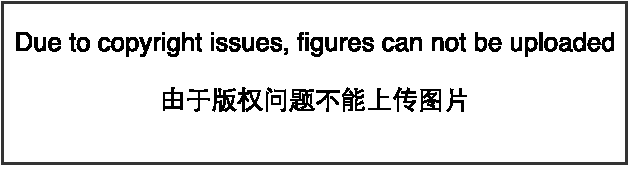
\includegraphics{figure.pdf}}
\else
\centerline{\includegraphics{Chapter1/figures/polar_color}}
\fi
\caption{TODO}
\label{fig:chap1_polar}
\end{figure}

许多\gls{AI}的任务都可以通过提取一个合适的特征集,然后将这些特征提供给简单的\gls{ML}算法来解决。
例如,从声音鉴别说话者的一个有用特征是说话者声道大小的估计。
这个特征为判断说话者是一个男性,女性还是儿童提供了有力线索。

然而,对于许多任务来说,很难知道应该提取哪些特征。
例如,假设我们想编写一个程序来检测照片中的车。
我们知道,汽车有轮子,所以我们可能会想用车轮的存在作为特征。
不幸的是,我们难以准确地从像素值的角度描述一个车轮看起来如何。
车轮具有简单的几何形状,但它的图像可以因为环境而变得很复杂,如落在车轮上的阴影、太阳照亮的车轮的金属零件、汽车的挡泥板或者遮挡的车轮一部分的前景物体,等等。

% -- 3 --

解决这个问题一个途径的是使用\gls{ML}来发现\gls{representation}本身,而不仅仅把表示映射到输出。
这种方法被称为\firstgls{representation_learning}。
学习到的表示往往获得比手动设计的表示更好的性能。
并且它们只需最少的人工干预, 就能让\glssymbol{AI}系统迅速适应新的任务。
\gls{representation_learning}算法只需几分钟就可以为简单的任务发现一个很好的特征集,对于复杂任务则需要几小时到几个月。
手动为一个复杂的任务设计特征需要耗费大量的人工时间和精力;甚至需要花费整个社群研究人员几十年时间。

一个\gls{representation_learning}算法的典型例子是\firstgls{AE}。
\gls{AE}是组合了将输入转换到不同表示\firstgls{encoder}函数和将新的表示转回原来形式的\firstgls{decoder}函数。 
\gls{AE}的训练目标是,输入经过\gls{encoder}和\gls{decoder}之后尽可能多的保留信息,同时希望新的\gls{representation}有各种好的属性。不同种类的\gls{AE}的目标是实现不同种类的属性。

当设计特征或学习特征的算法时,我们的目标通常是分离出能解释观察数据的\textbf{变化因素}(factors of variation)。
在此背景下,``因素''这个词仅指代的影响不同来源;因素通常不是乘性组合。
这些因素通常是不能被直接观察到的量。
相反,他们可能是现实世界中观察不到的物体或者不可观测的力,但影响能观测到的量。
他们还存在于人类的思维构造中,为了给观察到的数据提供有用的简化解释或推断原因。
它们可以被看作帮助我们了解富有变化的数据的概念或者抽象。
当分析语音记录时,变化的因素包括说话者的年龄、性别、他们的口音和他们正在说的词语。
当分析汽车的图像时,变化的因素包括汽车的位置、它的颜色、太阳的角度和亮度。

% -- 4 --

在许多现实世界的\gls{AI}应用困难的一个重要原因是很多因素的变化影响着我们能够观察到的每一个数据。
在夜间,一张图片中红色汽车的单个像素可能是非常接近黑色。
汽车轮廓的形状取决于视角。
大多数应用程序需要我们\emph{理清}变化的因素并丢弃我们不关心的因素。

当然,从原始数据中提取这样的高层次、抽象的特征是非常困难的。
许多这样的变化因素,诸如说话者的口音,只能对数据进行复杂的、接近人类水平的理解来确定。
它几乎与获得原来问题的表示一样困难,乍一看,\gls{representation_learning}似乎并不能帮助我们。

\firstgls{DL}通过其它较简单的表示来表达复杂表示,解决了\gls{representation_learning}中核心问题。

\gls{DL}让计算机通过较简单概念构建复杂的概念。
\figref{fig:chap1_deep_learning}显示了\gls{DL}系统通过组合较简单的概念,例如转角和轮廓,转而定义边缘来表示图像中一个人的概念。
\begin{figure}[!htb]
\ifOpenSource
\centerline{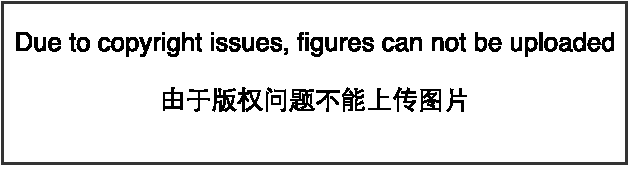
\includegraphics{figure.pdf}}
\else
\centerline{\includegraphics{Chapter1/figures/deep_learning}}
\fi
\caption{TODO}
\label{fig:chap1_deep_learning}
\end{figure}
\gls{DL}模型的典型例子是前馈深度网络或\firstacr{MLP}。
\gls{MLP}仅仅是一个将一组输入值映射到输出的数学函数。
该函数由许多较简单的函数组合而构成。
我们可以认为每个应用具有不同的数学函数,并为输入提供新的表示。

学习数据的正确表示的想法是解释\gls{DL}的一个观点。
另一个观点是深度允许计算机学习一个多步骤的计算机程序。
表示的每一层可以被认为是并行执行另一组指令后计算机的存储器状态。
更深的网络可以按顺序执行更多的指令。
顺序指令提供了极大的能力,因为后面的指令可以参考早期指令的结果。
根据\gls{DL}这个观点,一层的激活函数没有必要对解释输入变化的因素进行编码。
\gls{representation}还存储着协助程序执行的状态信息,使输入更加有意义。
这里的状态信息是类似于传统计算机程序中的计数器或指针。
它与具体的输入内容无关,但有助于模型组织其处理过程。

% -- 6 --

主要有两种测量模型深度的方式。
第一观点是基于评估架构所需执行的顺序指令的数目。
我们可以认为这是描述每个给定输入后,计算模型输出的流程图的最长路径。
正如两个等价的计算机程序根据不同的语言将具有不同的长度,相同的函数可以被绘制为具有不同深度的流程图,这取决于我们允许使用的单一步骤的函数。
\figref{fig:chap1_language}说明了语言的选择怎样给相同的架构两个不同的衡量。
\begin{figure}[!htb]
\ifOpenSource
\centerline{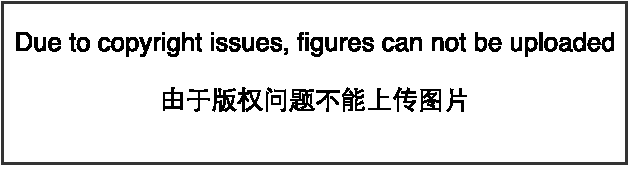
\includegraphics{figure.pdf}}
\else
\centerline{\includegraphics{Chapter1/figures/language}}
\fi
\caption{TODO}
\label{fig:chap1_language}
\end{figure}

另一种是在深度概率模型中使用的方法,不是将计算图的深度视为模型深度,而是将描述概念如何彼此相关的图的深度视为模型深度。
在这种情况下,计算每个概念表示的计算流程图的深度可能比概念本身的图更深。
这是因为系统对较简单概念的理解可以在给出更复杂概念的信息后进一步细化。
例如,一个\glssymbol{AI}系统观察一张其中一只眼睛在阴影中的脸部图像,最初可能只看到一只眼睛。
当检测到的脸部的存在后,它可以推断的第二只眼睛也可能是存在的。
在这种情况下,概念的图仅包括两层——关于眼睛的层和关于脸的层,但是,如果我们根据每个概念给出的其它$n$次估计进行改进,计算的图将包括$2n$个层。

% -- 7 --

由于并不总是清楚计算图的深度或概率模型图的深度哪一个是最相关的,并且由于不同的人选择不同的最小元素集来构建相应的图,导致架构的深度不存在单一的正确值,就像计算机程序的长度不存在单一的正确值。
也不存在模型多么深才能被修饰为``深''的共识。
<BAD>但是,\gls{DL}可以可靠地被视为比传统机器学习涉及更大量的学到函数或学到概念组合的模型的研究。

总之, 这本书的主题——\gls{DL}是\glssymbol{AI}的途径之一。
具体地讲,它是\gls{ML}的一种,一种允许计算机系统能从经验和数据中得到提高的技术。

我们主张\gls{ML}是构建能在复杂实际环境下运行的\glssymbol{AI}系统的唯一可行方法。
\gls{DL}是一种特定类型的\gls{ML},通过将世界表示为由较简单概念定义复杂概念,从一般抽象到高级抽象的嵌套概念体系获得极大的能力和灵活性。
\figref{fig:chap1_venn}说明了这些不同的\glssymbol{AI}学科之间的关系。\figref{fig:chap1_which_part_learned}给出了每个学科如何工作的一个高层次的原理。
\begin{figure}[!hbt]
\ifOpenSource
\centerline{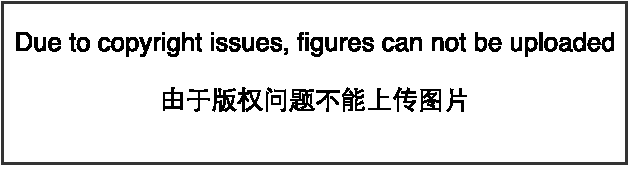
\includegraphics{figure.pdf}}
\else
\centerline{\includegraphics{Chapter1/figures/venn}}
\fi
\caption{TODO}
\label{fig:chap1_venn}
\end{figure}
\begin{figure}[!htb]
\ifOpenSource
\centerline{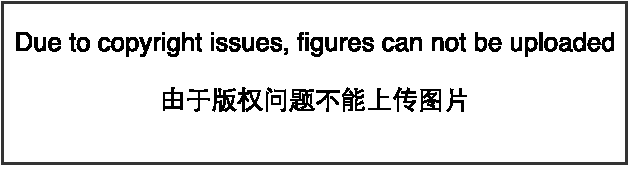
\includegraphics{figure.pdf}}
\else
\centerline{\includegraphics{Chapter1/figures/which_part_learned}}
\fi
\caption{TODO}
\label{fig:chap1_which_part_learned}
\end{figure}

\section{谁应该读这本书?}
\label{sec:who_should_read_this_book}

这本书对各类读者都一定用处的,但我们是基于两个主要目标受众而写的。
其中一个目标受众是学习\gls{ML}的大学生(本科或研究生),包括那些开始了职业生涯的\gls{DL}和\gls{AI}研究者。
另一个目标群体是没有\gls{ML}或统计背景但要迅速在他们的产品或平台开始使用\gls{DL}的软件工程师。
\gls{DL}在许多软件领域都已被证明是有用的,包括计算机视觉、语音和音频处理、自然语言处理、机器人技术、生物信息学和化学、电子游戏、搜索引擎、网络广告和金融。

% -- 8 --

为了最好地适应各类读者,这本书被组织为三个部分。
第一部分介绍了基本的数学工具和\gls{ML}的概念。
<BAD>第二部分介绍了本质上已解决的技术、最成熟的\gls{DL}算法。
第三部分介绍了被广泛认为是深度学习未来研究重点的但更具猜测性的想法。

读者可以随意跳过不感兴趣或与自己背景不相关的部分。
熟悉线性代数、概率和基本\gls{ML}概念的读者可以跳过第一部分,例如,当读者只是想实现一个能工作的系统则不需要阅读超出第二部分的内容。
为了帮助读者选择章节,\figref{fig:chap1_dependency}展示了这本书的高层组织结构的流程图。
\begin{figure}[!htb]
\ifOpenSource
\centerline{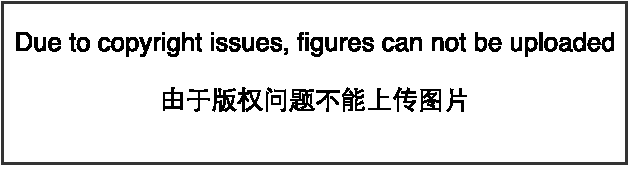
\includegraphics{figure.pdf}}
\else
\centerline{\includegraphics{Chapter1/figures/dependency}}
\fi
\caption{TODO}
\label{fig:chap1_dependency}
\end{figure}

% -- 10 --

我们假设所有读者都具备计算机科学背景。
也假设读者熟悉编程,并且对计算的性能问题、复杂性理论、入门级微积分和一些图论的术语有基本的了解。

\section{深度学习的历史趋势}
\label{sec:historical_trends_in_deep_learning}
通过历史背景了解\gls{DL}是最简单的方式。
我们指出了\gls{DL}的几个关键趋势,而不是提供详细的历史:
\begin{itemize}
 \item \gls{DL}有着悠久而丰富的历史,但伴随着很多反映不同哲学观点名称的尘封而渐渐消逝。
 \item 可用的训练数据的量已经增加,使得\gls{DL}变得更加有用。
 \item 随着时间的推移,针对\gls{DL}的计算机软硬件基础设施都有所改善,\gls{DL}模型的规模也随之增长。
 \item \gls{DL}已经解决日益复杂的应用,并随着时间的推移,精度不断提高。
\end{itemize}

\subsection{神经网络的众多名称和命运变迁}
\label{sec:the_many_names_and_changing_fortunes_of_neural_networks}

我们期待这本书的许多读者都听说过\gls{DL}这一激动人心的新技术,并为一本书提及关于一个新兴领域的``历史''而感到惊讶。
事实上,\gls{DL}的历史可以追溯到20世纪40年代。
\gls{DL}只是\emph{看上去像}一个新的领域,因为在目前流行的前几年它是相对冷门的,同时也因为它被赋予了许多不同的已经消逝的名称,最近才成为所谓的``深度学习''。
这个领域已经更换了很多名称,反映了不同的研究人员和不同观点的影响。

讲述整个综合性的\gls{DL}历史超出了本书的范围。
然而,一些基本的背景对理解\gls{DL}是有用的。
一般来说,目前为止已经有三次\gls{DL}的发展浪潮:在20世纪40年代到60年代\gls{DL}被称为\firstgls{cybernetics},20世纪80年代到90年代\gls{DL}被誉为\firstgls{connectionism},并于2006年开始,\gls{DL}在当前的名称下开始复苏。
这在\figref{fig:chap1_cybernetics_connectionism_ngrams_color}中定量给出。
\begin{figure}[!htb]
\ifOpenSource
\centerline{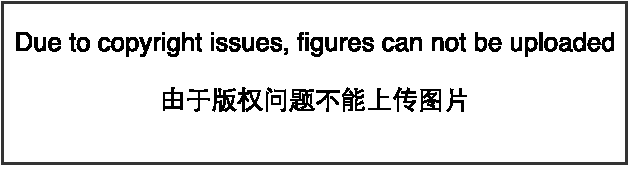
\includegraphics{figure.pdf}}
\else
\centerline{\includegraphics{Chapter1/figures/cybernetics_connectionism_ngrams_color}}
\fi
\caption{TODO}
\label{fig:chap1_cybernetics_connectionism_ngrams_color}
\end{figure}

% -- 12 --

我们现在认识的一些最早的学习算法,旨在模拟生物学习的计算模型,即大脑怎样学习或为什么能学习的模型。
其结果是,已经消逝的\gls{DL}的名称之一——\firstacr{ANN}。
此时\gls{DL}模型对应的观点是他们设计的系统是受生物大脑(无论人类大脑或其他动物的大脑)所启发。
尽管有些\gls{ML}的\gls{NN}有时被用来理解大脑功能\citep{hinton1991lesioning},它们一般都没有被设计成生物功能的真实模型。
\gls{DL}的神经观点受两个主要思想启发的。
一个想法是,大脑这个例子证明智能行为的可能性,因此建立智能概念上的直接途径是逆向大脑背后的计算原,并复制其功能。
另一种看法是,理解大脑和人类智力背后的原则将是非常有趣的,因此\gls{ML}模型除了解决工程应用的能力, 如果能阐明这些基本的科学问题也将会很有用。 

% -- 13 --
  
现代术语``\gls{DL}''超越了目前\gls{ML}模型的神经科学观点。
学习的\emph{多层次组合}这一更普遍的原则更加吸引人,这可以应用于\gls{ML}框架且不必是受神经启发的。
 
 
现代\gls{DL}的最早前身是从神经科学的角度出发的简单线性模型。
这些模型被设计为使用一组$\Sn$个输入$\Sx_1, \dots ,\Sx_n$并将它们与一个输出$\Sy$相关联。 
这些模型将学习一组权重$\Sw_1, \dots, \Sw_n $ 并计算它们的输出$f(\Vx, \Vw) = \Sx_1 \Sw_1 + \dots + \Sx_n \Sw_n$。
这第一波\gls{NN}研究的浪潮被称为\gls{cybernetics},如\figref{fig:chap1_cybernetics_connectionism_ngrams_color}所示。

\ENNAME{McCulloch-Pitts}神经元\citep{McCulloch43}是脑功能的早期模型。
该线性模型通过测试函数$f(\Vx,\Vw)$的是正还是负来识别两种不同类型的输入。
当然,为了使模型对应于期望的类别定义,需要正确地设置权重。
这些权重可以由操作人员设定。
在20世纪50年代,感知机\citep{Rosenblatt-1956,Rosenblatt-1958}成为第一个能根据了每个类别输入的\gls{example}来学习权重的模型。
约在同一时期,\textbf{自适应线性元件}(ADALINE),简单地返回函数$f(\Vx)$本身的值来预测一个实数\citep{Widrow60},并且还可以学习从数据预测这些数。

这些简单的学习算法大大影响了\gls{ML}的现代景象。
用于调节ADALINE的权重的训练算法是称为\firstgls{SGD}的一种特例。
稍加修改的\gls{SGD}算法仍然是当今\gls{DL}的主要训练算法。

基于感知机和ADALINE中使用的函数$f(\Vx, \Vw)$的模型被称为\firstgls{linear_model}。
这些模型仍然是最广泛使用的\gls{ML}模型,尽管在许多情况下,它们以不同于原始模型的方式进行\emph{训练}。

\gls{linear_model}有很多局限性。
最著名的是,它们无法学习XOR函数,即$f([0,1], \Vw) = 1, f([1,0], \Vw)=1$, 
但是$f([1,1], \Vw)=0, f([0,0],\Vw)= 0$。
在\gls{linear_model}中观察到这些缺陷的评论家开始反对受生物学启发的学习\citep{Minsky69}。
这是\gls{NN}第一次热度较多的下降。

现在,神经科学被视为\gls{DL}研究的一个重要灵感来源,但它已不再是该领域的主要导向。

% -- 14 --

如今神经科学在\gls{DL}研究中的作用被削弱,主要的原因只是我们根本没有足够的关于大脑信息来作为指导。
要获得对大脑实际使用算法的深刻理解,我们需要有能力同时监测(至少是)数千相连神经元的活动。
我们不能够做到这一点,甚至连大脑的最简单、最深入研究的部分我们都还远远没有理解\citep{olshausen:2005}。

神经科学已经给了我们依靠单一\gls{DL}算法解决许多不同任务的理由。
神经学家们发现,如果将雪貂的大脑重新连接,使视觉信号传送到听觉区域,它们可以学会用大脑的听觉处理区域``看''\citep{von2000visual}。
这表明,多数哺乳动物大脑的可能使用单一的算法解决大部分大脑可以解决的不同任务。
这个假设之前,\gls{ML}研究更加分散,研究人员在不同的社区研究自然语言处理、计算机视觉、运动规划和语音识别。
如今,这些应用的社区仍然是独立的,但是\gls{DL}研究小组同时研究许多或甚至所有这些应用领域是很常见的。

我们能够从神经科学得到一些粗略的指南。
仅通过计算单元之间的相互作用而变得智能的基本思想是受大脑启发的。
新认知机\citep{Fukushima80}受哺乳动物视觉系统的结构启发,引入了一个处理图片的强大模型架构,后来成为了现代卷积网络的基础\citep{LeCun98-small},我们将会在\secref{sec:the_neuroscientific_basis_for_convolutional_networks}看到。
目前大多数\gls{NN}基于称为\firstgls{ReLU}的神经单元模型。
原始认知机\citep{Fukushima75}受我们关于大脑功能知识的启发, 引入了一个更复杂的版本。
简化的现代版基于许多观点进化发展,\citet{Nair-2010}和\citet{Glorot+al-AI-2011-small}援引神经科学作为影响,\citet{Jarrett-ICCV2009}援引更多面向工程的影响。
虽然神经科学是灵感的重要来源,它不需要被视为刚性指导。
我们知道,实际的神经元与现代\gls{ReLU}计算着非常不同函数,但更接近真实神经网络的系统并没有导致\gls{ML}性能的提升。
此外,虽然神经科学已经成功地启发了一些\gls{NN}\emph{架构},但我们还没有足够的了解生物学习的神经科学,因此在训练这些架构时,不能提供给我们很多关于\emph{学习算法}的指导。

媒体报道经常强调\gls{DL}与大脑的相似性。
虽然\gls{DL}研究人员更可能比其他\gls{ML}领域(如核机器或贝叶斯统计工作的研究人员)引用大脑作为影响,人们不应该认为\gls{DL}是对模拟大脑的尝试。
现代\gls{DL}从许多领域获取灵感,特别是应用数学的基本内容如线性代数、概率论、信息论和数值优化。
虽然一些\gls{DL}的研究人员引用神经科学作为灵感的重要来源,但其他学者完全不关心神经科学。

% -- 15 --

值得注意的是,了解大脑是如何在算法层面上工作的尝试是鲜活且发展良好的。
这项尝试主要是被称为``计算神经科学'',并且是独立于\gls{DL}一个领域。
研究人员两个领域之间反复研究是很常见的。
\gls{DL}领域主要是关注如何构建智能的计算机系统,用来解决需要智能才能解决的任务,而计算神经科学领域主要是关注构建大脑如何工作的更精确的模型。

在20世纪80年代,神经网络研究的第二次浪潮在很大程度上是伴随一个被称为\firstgls{connectionism}或\textbf{并行分布处理}运动而出现的\citep{Rumelhart86,mcclelland1995appeal}。
\gls{connectionism}是在认知科学的背景下出现的。
认知科学是理解心智,并结合多个不同层次分析的跨学科方法。
在20世纪80年代初期,大多数认知科学家研究符号推理的模型。
尽管这很流行,符号模型很难解释大脑如何真正使用神经元实现推理功能。 
连接主义者开始研究实际能基于神经实现的认知模型\citep{Touretzky1985},其中很多复苏的想法可以追溯到心理学家\ENNAME{Donald Hebb}在20世纪40年代的工作\citep{Hebb49}。

\gls{connectionism}的中心思想是,当网络将大量简单计算单元连接在一起时可以实现智能行为。
这种见解同样适用于与计算模型中隐层单元类似作用的生物神经系统中的神经元。  

上世纪80年代的\gls{connectionism}运动过程中形成的几个关键概念在今天的\gls{DL}中仍然是非常重要的。

其中一个概念是\firstgls{distributed_representation}\citep{Hinton-et-al-PDP1986}。
这一想法是,系统每个的输入应该由许多特征表示的,并且每个特征应参与许多可能输入的表示。
例如,假设我们有一个能够识别红色、绿色、或蓝色的汽车、卡车和鸟类的视觉系统。
表示这些输入的其中一个方法是将九个可能的组合:红卡车,红汽车,红鸟,绿卡车等等使用单独的神经元或\gls{hidden_unit}激活。
这需要九个不同的神经元,并且每个神经必须独立地学习颜色和对象身份的概念。
改善这种情况的方法之一是使用\gls{distributed_representation},即用三个神经元描述颜色,三个神经元描述对象身份。 
这仅仅需要6个神经元而不是9个,并且描述红色的神经元能够从汽车、卡车和鸟类的图像中学习红色,而不仅仅是从一个特定类别的图像中学习。 
\gls{distributed_representation}的概念是本书的核心,我们将在\chapref{chap:representation_learning}中更加详细地描述。

% -- 16 --

\gls{connectionism}运动的另一个重要成就是反向传播算法的成功运用(训练具有内部表示的深度\gls{NN})和普及\citep{RHW,Lecun-these87}。
这个算法虽然已经黯然失色不再流行,但截至写书之时,仍是训练深度模型的主要方法。

在20世纪90年代,研究人员在使用\gls{NN}进行序列建模的方面取得了重要进展。
\citet{Hochreiter91}和\citet{Bengio1994ITNN}指出了建模长序列的一些根本数学难题,将在\secref{sec:the_challenge_of_long_term_dependencies}中描述。
\citet{Hochreiter+Schmidhuber-1997}引入\gls{LSTM}(\glssymbol{LSTM})网络来解决这些难题。
如今,\glssymbol{LSTM}在许多序列建模任务中广泛应用,包括Google的许多自然语言处理任务。

\gls{NN}研究的第二次浪潮一直持续到上世纪90年代中期。
基于\gls{NN}等其他\glssymbol{AI}技术的企业开始在寻求投资的同时,做不切实际野心勃勃的主张。
当\glssymbol{AI}研究不能实现这些不合理的期望时,投资者感到失望。
同时,\gls{ML}的其他领域取得进步。
核学习机\citep{Boser92,Cortes95,SchBurSmo99}和图模型\citep{Jordan98}都在很多重要任务上实现了很好的效果。
这两个因素导致了\gls{NN}热度的第二次下降,一直持续到2007年。

在此期间,\gls{NN}持续在某些任务上获得令人印象深刻的表现\citep{LeCun98-small,Bengio-nnlm2001}。
加拿大高级研究所(CIFAR)通过其神经计算和自适应感知(NCAP)研究计划帮助维持\gls{NN}研究。
这个计划统一了由分别由\ENNAME{Geoffrey Hinton},\ENNAME{Yoshua Bengio}和\ENNAME{Yann LeCun}引导的多伦多大学、蒙特利尔大学和纽约大学的\gls{ML}研究小组。
CIFAR NCAP研究计划具有多学科的性质,其中还包括在人类神经科学家和计算机视觉专家。

% -- 17 --

在那个时间点上,普遍认为深度网络被难以训练的。
现在我们知道,从20世纪80年代就存在的算法能工作得非常好,但是直到在2006年前后都没有体现出来。
这个问题可能是单纯的因为计算复杂性太高,而以当时可用的硬件难以进行足够的实验。

神经网络研究的第三次浪潮开始于2006年的突破。
\ENNAME{Geoffrey Hinton}表明名为\gls{DBN}的\gls{NN}可以使用一种称为贪婪逐层训练的策略进行有效地训练\citep{Hinton06},我们将在\secref{sec:greedy_layer_wise_unsupervised_pretraining}中更详细地描述。
CIFAR附属的其他研究小组很快表明,同样的策略可以被用来训练许多其他类型的深度网络\citep{Bengio+Lecun-chapter2007-small,ranzato-07},并能系统地帮助提高在测试样例上的泛化能力。
\gls{NN}研究的这一次浪潮普及了``\gls{DL}''这一术语的使用,强调研究人员现在可以训练以前不可能训练的更深的神经网络,并把注意力集中于深度的理论意义\citep{Bengio+Lecun-chapter2007,Delalleau+Bengio-2011-small,Pascanu-et-al-ICLR2014,Montufar-et-al-NIPS2014}。
此时,深度\gls{NN}已经优于与之竞争的基于其他\gls{ML}技术以及手工设计函数的\glssymbol{AI}系统。
神经网络流行的第三次浪潮在写这本书的时候还在继续,尽管深度学习的研究重点在这一段时间内发生了巨大变化。
第三次浪潮开始把重点放在新的无监督学习技术和深度模型从小数据集进行推广的能力,但现在更多的注意点是在更古老的监督学习算法和深度模型充分利用大型标注数据集的能力。

\subsection{与日俱增的数据量}
\label{sec:increasing_dataset_sizes}
人们可能想问,尽管人工\gls{NN}的第一个实验在20世纪50年代就完成了,为什么\gls{DL}直到最近才被认为是关键技术。
自20世纪90年代以来,\gls{DL}就已经成功用于商业应用,但通常被视为是一种艺术而不是一种技术,且只有专家可以使用的艺术,这种观点持续到最近。
确实,要从一个\gls{DL}算法获得良好的性能需要一些技巧。
幸运的是,随着训练数据的增加,所需的技巧正在减少。
目前在复杂的任务达到与人类表现的学习算法,与20世纪80年代努力解决的玩具问题(toy problem)的学习算法几乎是一样的,尽管这些算法训练的模型经历了变革,简化了极深架构的训练。
最重要的新进展是现在我们有了这些算法成功训练所需的资源。
\figref{fig:chap1_dataset_size_color}展示了基准数据集的大小如何随着时间的推移显着增加。
这种趋势是由社会日益数字化驱动的。
由于我们的活动越来越多发生在计算机上,我们做什么也越来越多地被记录。
我们的计算机越来越多地联网在一起,变得更容易集中管理这些记录,并将它们整理成适于\gls{ML}应用的数据集。
因为``大数据''的时代\gls{ML}要容易得多,因为统计估计的主要负担——观察少量数据以在新数据上泛化——已经减轻。
截至2016年,一个粗略的经验法则是,监督\gls{DL}算法一般在每类给定约5000标注样本情况下可以实现可接受的性能,当至少有1000万标注样本的数据集用于训练时将达到或超过人类表现。
<BAD>在更小的数据集上成功工作是一个重要的研究领域,我们应特别侧重于如何通过无监督或半监督学习充分利用大量的未标注样本。
\begin{figure}[!htb]
\ifOpenSource
\centerline{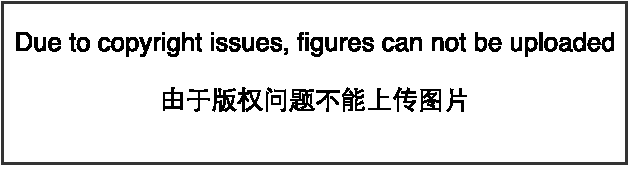
\includegraphics{figure.pdf}}
\else
\centerline{\includegraphics{Chapter1/figures/dataset_size_color}}
\fi
\caption{TODO}
\label{fig:chap1_dataset_size_color}
\end{figure}
\begin{figure}[!htb]
\ifOpenSource
\centerline{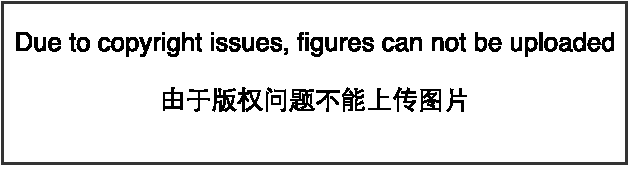
\includegraphics{figure.pdf}}
\else
\centerline{\includegraphics[width=0.8\textwidth]{Chapter1/figures/mnist}}
\fi
\caption{TODO}
\label{fig:chap1_mnist}
\end{figure}

% -- 20 --

\subsection{与日俱增的模型规模}
\label{sec:increasing_model_sizes}

相对20世纪80年代较少的成功,现在\gls{NN}非常成功的另一个重要原因是现在我们拥有的计算资源可以运行更大的模型。
\gls{connectionism}的主要见解之一是,当动物的许多神经元一起工作时会变得聪明。
单独神经元或小集合的神经元不是特别有用。

生物神经元没有连接的特别密集。
如\figref{fig:chap1_number_of_synapses_color}所示,几十年来,我们的\gls{ML}模型中每个神经元的连接数量甚至与哺乳动物大脑的在同一数量级。
\begin{figure}[!htb]
\ifOpenSource
\centerline{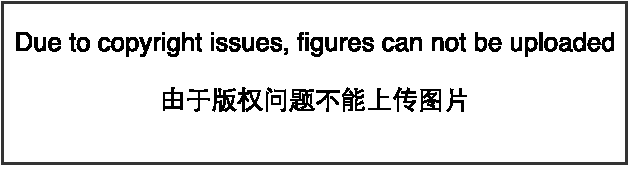
\includegraphics{figure.pdf}}
\else
\centerline{\includegraphics{Chapter1/figures/number_of_synapses_color}}
\fi
\caption{TODO}
\label{fig:chap1_number_of_synapses_color}
\end{figure}

如\figref{fig:chap1_number_of_neurons_color}所示,就神经元的总数目而言,直到最近\gls{NN}都是惊人的少。
自从引入\gls{hidden_unit}以来,人工\gls{NN}的规模大约每2.4年扩大一倍。
这种增长是由更大内存、更快的计算机和更大的可用数据集驱动的。
较大的网络能够在更复杂的任务中实现更高的精度。
这种趋势看起来将持续数十年。
除非有允许迅速扩展的新技术,否则至少直到21世纪50年代,人工\gls{NN}将才能具备与人脑相同数量级的神经元。
生物神经元表示的函数可能比目前的人工神经元更复杂,因此生物神经网络可能比图中描绘的更大。
\begin{figure}[!htb]
\ifOpenSource
\centerline{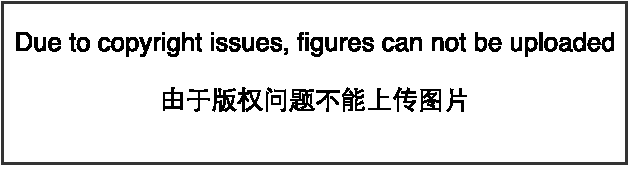
\includegraphics{figure.pdf}}
\else
\centerline{\includegraphics{Chapter1/figures/number_of_neurons_color}}
\fi
\caption{TODO}
\label{fig:chap1_number_of_neurons_color}
\end{figure}


现在回想起来,比一个水蛭的神经元还少的\gls{NN}不能解决复杂的\gls{AI}问题是不足为奇的。
即使是现在从一个计算系统角度来看可能相当大的网络, 实际上比相对原始的脊椎动物如青蛙的神经系统更小。

由于有更快的CPU、通用GPU的到来(在\secref{sec:gpu_implementations}中讨论)、更快的网络连接和更好的分布式计算的软件基础设施,模型的规模随着时间的推移不断增加是\gls{DL}历史中最重要的趋势之一。
普遍预计这种趋势将很好地持续到未来。

% -- 21 --

\subsection{与日俱增的精度、复杂度和对现实世界的冲击}
\label{sec:increasing_accuracy_complexity_and_real_world_impact}

<BAD>20世纪80年代以来,\gls{DL}一直在提高提供识别精度和预测的能力。
此外,\gls{DL}持续地被成功应用到越来越广泛的应用中去。

最早的深度模型被用来识别裁剪的很合适且非常小的图像中的单个对象\citep{Rumelhart86}。
自那时以来,\gls{NN}可以处理的图像尺寸逐渐增加。
现代对象识别网络能处理丰富的高分辨率照片,并且不要求在被识别的对象附近进行裁剪\citep{Krizhevsky-2012}。
类似地,最早网络只能识别两种对象(或在某些情况下,单一种类的对象的存在与否),而这些现代网络通常识别至少\NUMTEXT{1000}个不同类别的对象。
对象识别中最大的比赛是每年举行的ImageNet大型视觉识别挑战(ILSVRC)。
<BAD>\gls{DL}迅速崛起的一个戏剧性的时刻是卷积网络第一次大幅赢得这一挑战,将最高水准的前5错误率从\NUMTEXT{26.1\%}降到\NUMTEXT{15.3\%}\citep{Krizhevsky-2012},这意味着该卷积网络产生针对每个图像的可能类别的分级列表,尽管\NUMTEXT{15.3\%}的测试样例的正确类别不会出现在此列表中的前5。

此后,深度卷积网络一直能在这些比赛中取胜,截至写书时,\gls{DL}的进步将这个比赛中的前5错误率降到\NUMTEXT{3.6%}, 如\figref{fig:chap1_imagenet_color}所示。
\begin{figure}[!htb]
\ifOpenSource
\centerline{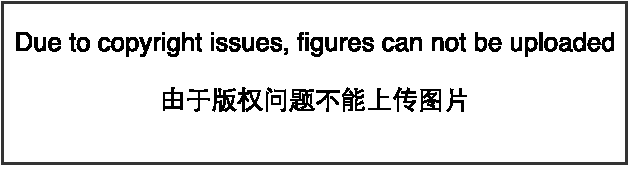
\includegraphics{figure.pdf}}
\else
\centerline{\includegraphics{Chapter1/figures/imagenet_color}}
\fi
\caption{TODO}
\label{fig:chap1_imagenet_color}
\end{figure}

% -- 23 --

\gls{DL}也对语音识别产生了巨大影响。
语音识别在20世纪90年代提高后,直到约2000年都停滞不前。
\gls{DL}的引入\citep{dahl2010phonerec,Deng-2010,Seide2011,Hinton-et-al-2012}导致语音识别错误率的陡然下降,有些错误率甚至降低了一半。 
我们将在\secref{sec:speech_recognition}更详细地探讨这个历史。

深度网络在行人检测和图像分割中也有引人注目的成功\citep{sermanet-cvpr-13,Farabet-et-al-2013,couprie-iclr-13},在交通标志分类上取得了超越人类的表现\citep{Ciresan-et-al-2012}。

在深度网络的规模和的精度有所提高的同时,它们可以解决的任务也日益复杂。
\citet{Goodfellow+et+al-ICLR2014a}表明,\gls{NN}可以学习输出描述图像的整个字符序列,而不是仅仅识别单个对象。
此前,人们普遍认为,这种学习需要对序列中的单个元素进行标注\citep{Gulcehre+Bengio-arxiv-2013}。
\gls{RNN},如之前提到的\glssymbol{LSTM}序列模型,现在用于建模序列和其他序列之间的关系,而不是仅仅固定输入之间的关系。
这个序列到序列的学习似乎处于另一个应用演进的浪尖:机器翻译\citep{Sutskever-et-al-NIPS2014,Bahdanau-et-al-ICLR2015-small}。

% -- 24 --

日益复杂的趋势已将其推向逻辑结论,即神经图灵机\citep{Graves-et-al-arxiv2014}的引入,它能学习读取存储单元和向存储单元写入任意内容。
这样的\gls{NN}可以从期望行为的\gls{example}中学习简单的程序。
例如,从杂乱和排好序的\gls{example}中学习对一系列数进行排序。
这种自我编程技术正处于起步阶段,但原则上未来可以适用于几乎所有的任务。


\gls{DL}的另一个冠军成就是在\firstgls{RL}领域的扩展。
在\gls{RL}的背景下,一个自主体必须通过试错来学习执行任务,而无需人类操作者的任何指导。
DeepMind表明,基于\gls{DL}的\gls{RL}系统能够学会玩Atari视频游戏,并在多种任务中可与人类匹敌\citep{Mnih-et-al-2015}。
\gls{DL}也显著改善了机器人\gls{RL}的性能\citep{finn2015learning}。

许多\gls{DL}应用都是高利润的。现在\gls{DL}被许多顶级的技术公司使用,包括Google、Microsoft、Facebook、IBM、Baidu、Apple、Adobe、Netflix、NVIDIA和NEC。

\gls{DL}的进步也严重依赖于软件基础架构的进展。
软件库如Theano\citep{bergstra+al:2010-scipy,Bastien-2012}、PyLearn2\citep{pylearn2_arxiv_2013}、Torch\citep{Torch-2011}、DistBelief\citep{Dean-et-al-NIPS2012}、Caffe\citep{Jia13caffe}、MXNet\citep{chen2015mxnet}和TensorFlow\citep{tensorflow}都能支持重要的研究项目或商业产品。

\gls{DL}也为其他科学做出了贡献。
识别对象的现代卷积网络提供给神经科学家可以研究的视觉处理模型\citep{dicarlo-tutorial-2013}。
\gls{DL}也为处理海量数据、在科学领域作出的有效预测提供了非常有用的工具。
它已成功地用于预测分子如何相互作用,这能帮助制药公司设计新的药物\citep{Dahl-et-al-arxiv2014}、搜索的亚原子粒子\citep{baldi2014searching}和自动解析用于构建人脑三维图的显微镜图像\citep{knowlesdeep}。
我们期待\gls{DL}未来出现在越来越多的科学领域。

% -- 25 --

总之,\gls{DL}是\gls{ML}的一种方法, 过去几十年的发展中,它深深地吸收了我们关于人脑、统计学与应用数学的知识。
近年来,\gls{DL}的普及性和实用性有了极大的发展,这在很大程度上得益于更强大的计算机、更大的数据集和能够训练更深网络的技术。
未来几年充满了进一步提高\gls{DL}并将它带到新领域挑战和机遇。

% -- 26 --

\part{应用数学与机器学习基础}
\label{part:applied_math_and_machine_learning_basics}
\part{深层网络:现代实践}
\label{part:deep_networks_modern_practices}

% !Mode:: "TeX:UTF-8"
% Translator: Kai Li
\chapter{\glsentrytext{deep_feedforward_network}}
\label{chap:deep_feedforward_networks}

\firstgls{deep_feedforward_network},也叫作\firstgls{feedforward_neural_network}或者\firstall{MLP},是典型的深度学习模型。\gls{feedforward_network}的目标是近似某个函数$f^*$。
例如,对于分类器,$y = f^*(\bm{x})$将输入$\bm{x}$映射到一个类别$y$。
\gls{feedforward_network}定义了一个映射$\bm{y} = f(\bm{x}; \bm{\theta})$,并且学习参数$\bm{\theta}$的值,使它能够得到最佳的函数近似。

这种模型被称为\firstgls{feedforward}的,是因为信息流过$\bm{x}$的函数,流经用于定义$f$的中间计算过程,最终到达输出$\bm{y}$。
%这里的feedforward是翻译成前向的,还是前馈的?
在模型的输出和模型本身之间没有\firstgls{feedback}连接。
当前馈神经网络被扩展成包含\gls{feedback}连接时,它们被称为\firstgls{RNN},在第\ref{chap:sequence_modeling_recurrent_and_recursive_nets}章介绍。

\gls{feedforward_network}对于机器学习的从业者是极其重要的。
它们是许多重要商业应用的基础。
例如,用于对照片中的对象进行识别的\gls{CNN}就是一种专门的\gls{feedforward_network}。
\gls{feedforward_network}是通往\gls{recurrent_network}之路的概念基石,后者在自然语言的许多应用中发挥着巨大作用。

\gls{feedforward_neural_network}被称作\firstgls{network}是因为它们通常用许多不同函数复合在一起来表示。
该模型与一个有向无环图相关联,而图描述了函数是如何复合在一起的。
例如,我们有三个函数$f^{(1)}, f^{(2)}$和$f^{(3)}$连接在一个链上以形成$f(\bm{x}) = f^{(3)}(f^{(2)}(f^{(1)}(\bm{x})) )$。
这些链式结构是神经网络中最常用的结构。
在这种情况下,$f^{(1)}$被称为网络的\firstgls{first_layer},$f^{(2)}$被称为\firstgls{second_layer},以此类推。
链的全长称为模型的\firstgls{depth}。
正是因为这个术语才出现了``深度学习''这个名字。
\gls{feedforward_network}的最后一层被称为\firstgls{output_layer}。
在神经网络训练的过程中,我们让$f(\bm{x})$去匹配$f^*(\bm{x})$的值。
训练数据为我们提供了在不同训练点上取值的、含有噪声的$f^*(\bm{x})$的近似实例。
每个样例$\bm{x}$都伴随着一个标签$y\approx f^*(\bm{x})$。
训练样例直接指明了输出层在每一点$\bm{x}$上必须做什么;它必须产生一个接近$y$的值。
但是训练数据并没有直接指明其他层应该怎么做。
学习算法必须决定如何使用这些层来产生想要的输出,但是训练数据并没有说每个单独的层应该做什么。
相反,学习算法必须决定如何使用这些层来最好地实现$f^*$的近似。
因为训练数据并没有给出这些层中的每一层所需的输出,所以这些层被称为\firstgls{hidden_layer}。

% -- 163 --

最后,这些网络被称为\emph{神经网络}是因为它们或多或少地受到神经科学的启发。
网络中的每个\gls{hidden_layer}通常都是向量值的。这些\gls{hidden_layer}的维数决定了模型的\firstgls{width}。
向量的每个元素都可以被视为起到类似一个神经元的作用。
除了将层想象成向量到向量的单个函数,我们也可以把层想象成由许多并行操作的\firstgls{unit}组成,每个单元表示一个向量到标量的函数。
每个单元在某种意义上类似一个神经元,它接收的输入来源于许多其他的单元,并且计算它自己的激活值。
使用多层向量值表示的想法来源于神经科学。
用于计算这些表示的函数$f^{(i)}(\bm{x})$的选择,也或多或少地受到神经科学观测的指引,这些观测是关于生物神经元计算功能的。
然而,现代的神经网络研究受到更多的是来自许多数学和工程学科的指引,并且神经网络的目标并不是完美地给大脑建模。
我们最好将\gls{feedforward_neural_network}想成是为了实现统计\gls{generalization}而设计出的函数近似机器,它偶尔从我们了解的大脑中提取灵感但是并不是大脑功能的模型。

一种理解\gls{feedforward_network}的方式是从线性模型开始,并考虑如何克服它的局限性。
线性模型,例如\gls{logistic_regression}和线性回归,是非常吸引人的,因为无论是通过闭解形式还是使用凸优化,它们都能高效而可靠地拟合。
线性模型也有明显的缺陷,那就是该模型的能力被局限在线性函数里,所以它无法理解任何两个输入变量间的相互作用。

为了扩展线性模型来表示$\bm{x}$的非线性函数,我们可以把线性模型不用在$\bm{x}$ 本身,而是用在一个变换后的输入$\phi(\bm{x})$上,这里$\phi$是一个非线性变换。
同样,我们可以使用\ref{sec:support_vector_machines}节中描述的\gls{kernel_trick},来得到一个基于隐含地使用$\phi$映射的非线性学习算法。
我们可以认为$\phi$提供了一组描述$\bm{x}$的特征,或者认为它提供了$\bm{x}$的一个新的表示。

% -- 164 --

剩下的问题就是如何选择映射$\phi$。
\begin{enumerate}
\item 其中一种选择是使用一个通用的$\phi$,例如无限维的$\phi$,它隐含地用在基于\glssymbol{RBF}核的\gls{kernel_machines}上。
如果$\phi(\bm{x})$具有足够高的维数,我们总是有足够的能力来拟合训练集,但是对于测试集的\gls{generalization}往往不佳。
非常通用的特征映射通常只基于局部光滑的原则,并没有将足够的先验信息进行编码来解决高级问题。

\item 另一种选择是手动地设计$\phi$。
在深度学习出现以前,这都是主流的方法。
这种方法对于每个单独的任务都需要人们数十年的努力,从业者各自擅长特定的领域(如语音识别或计算机视觉),并且不同领域之间很难迁移(transfer)。

\item 深度学习的策略是去学习$\phi$。
在这种方法中,我们有一个模型$y = f(\bm{x};\theta, \bm{w}) = \phi(\bm{x}; \theta)^\top \bm{w}$。
我们现在有两种参数:用于从一大类函数中学习$\phi$的参数$\bm{\theta}$,以及用于将$\phi(\bm{x})$映射到所需的输出的参数$\bm{w}$。
这是\gls{deep_feedforward_network}的一个例子,其中$\phi$定义了一个\gls{hidden_layer}。
这是三种方法中唯一一种放弃训练问题的凸性的方法,但是利大于弊。
在这种方法中,我们将表示参数化为$\phi(\bm{x}; \bm{\theta})$,并且使用优化算法来寻找$\bm{\theta}$,使它能够得到一个好的表示。
如果我们想要的话,这种方法也可以通过使它变得高度通用以获得第一种方法的优点——我们只需使用一个非常广泛的函数族$\phi(\bm{x}; \bm{\theta})$。
这种方法也可以获得第二种方法的优点。
人类专家可以将他们的知识编码进网络来帮助\gls{generalization},他们只需要设计那些他们期望能够表现优异的函数族$\phi(\bm{x}; \bm{\theta})$即可。
这种方法的优点是人类设计者只需要寻找正确的函数族即可,而不需要去寻找精确的函数。
\end{enumerate}

这种通过学习特征来改善模型的一般化原则不止适用于本章描述的\gls{feedforward_neural_network}。
它是深度学习中反复出现的主题,适用于全书描述的所有种类的模型。
\gls{feedforward_neural_network}是这个原则的应用,它学习从$\bm{x}$到$\bm{y}$的确定性映射并且没有反馈连接。
后面出现的其他模型会把这些原则应用到学习随机映射、学习带有反馈的函数以及学习单个向量的概率分布。

% -- 165 --

本章我们先从\gls{feedforward_network}的一个简单例子说起。
接着,我们讨论部署一个\gls{feedforward_network}所需的每个设计决策。
首先,训练一个\gls{feedforward_network}至少需要做和线性模型同样多的设计决策:选择一个优化模型,代价函数以及输出单元的形式。
我们先回顾这些基于梯度学习的基本知识,然后去面对那些只出现在\gls{feedforward_network}中的设计决策。
\gls{feedforward_network}已经引入了\gls{hidden_layer}的概念,这需要我们去选择用于计算\gls{hidden_layer}值的\firstgls{activation_function}。
我们还必须设计网络的结构,包括网络应该包含多少层、这些层应该如何连接,以及每一层包含多少单元。
在深度神经网络的学习中需要计算复杂函数的梯度。
我们给出\firstgls{back_propagation}算法和它的现代推广,它们可以用来高效地计算这些梯度。
最后,我们以某些历史观点来结束这一章。

\section{实例:学习XOR}
\label{sec:example_learning_xor}

为了使\gls{feedforward_network}的想法更加具体,我们首先从一个可以完整工作的\gls{feedforward_network}说起,这个例子解决一个非常简单的任务:学习XOR函数。

XOR函数(``异或''逻辑)是两个二进制值$x_1$和$x_2$的运算。
当这些二进制值中恰好有一个为1时,XOR函数返回值为1。
其余情况下返回值为0。
XOR函数提供了我们想要学习的目标函数$y = f^*(\bm{x})$。
我们的模型给出了一个函数$y=f(\bm{x}; \bm{\theta})$并且我们的学习算法会不断调整参数$\bm{\theta}$来使得$f$尽可能接近$f^*$。

在这个简单的例子中,我们不会关心统计\gls{generalization}。
我们希望网络在这四个点$\SetX =\{[0, 0]^\top, [0, 1]^\top, [1, 0]^\top, [1, 1]^\top\}$上表现正确。
我们会用全部这四个点来训练我们的网络,唯一的挑战是拟合训练集。

我们可以把这个问题当作是回归问题,并使用\gls{mean_squared_error}损失函数。
我们选择这个损失函数是为了尽可能简化本例中用到的数学。
在应用领域,对于二进制数据建模时,\glssymbol{mean_squared_error}通常并不是一个合适的损失函数。
更加合适的方法将在\ref{sec:sigmoid_units_for_bernoulli_output_distributions}节中讨论。

% -- 166 --

评估整个训练集上表现的\glssymbol{mean_squared_error}损失函数为
\begin{equation}
J(\bm{\theta}) = \frac{1}{4} \sum_{\bm{x}\in \SetX} (f^*(\bm{x}) - f(\bm{x}; \bm{\theta}))^2.
\end{equation}

我们现在必须要选择我们模型$f(\bm{x}; \bm{\theta})$的形式。
假设我们选择一个线性模型,$\bm{\theta}$包含$\bm{w}$和$b$,那么我们的模型被定义成
\begin{equation}
f(\bm{x}; \bm{w}, b) = \bm{x}^\top \bm{w} + b.
\end{equation}
我们可以用\gls{normal_equations}对$\bm{w}$和$b$最小化$J(\bm{\theta})$,来得到一个闭式解。

解\gls{normal_equations}以后,我们得到$\bm{w} = 0$以及$b = \frac{1}{2}$。
线性模型仅仅是在任意一点都输出0.5。
为什么会发生这种事?
图\ref{fig:chap6_xor_space_gray}演示了线性模型为什么不能用来表示XOR函数。
解决这个问题的其中一种方法是使用一个模型来学习一个不同的特征空间,在这个空间上线性模型能够表示这个解。
% fig 6.1
\begin{figure}[!htb]
\ifOpenSource
\centerline{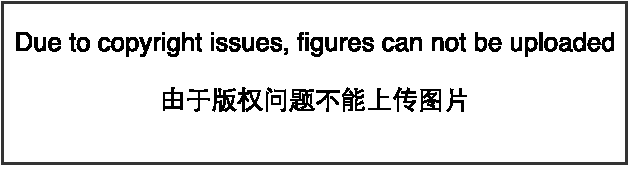
\includegraphics{figure.pdf}}
\else
\centerline{\includegraphics{Chapter6/figures/xor_space_gray}}
\fi
\captionsetup{singlelinecheck=off}
\caption{通过学习一个表示来解决XOR问题。
图上的粗体数字标明了学得的函数必须在每个点输出的值。
\emph{(左)}直接应用于原始输入的线性模型不能实现XOR函数。
当$x_1 = 0$时,模型的输出必须随着$x_2$的增大而增大。
当$x_1 = 1$时,模型的输出必须随着$x_2$的增大而减小。
线性模型必须对$x_2$使用固定的系数$w_2$。
因此,线性模型不能使用$x_1$的值来改变$x_2$的系数,从而不能解决这个问题。 
\emph{(右)}在由神经网络提取的特征表示的变换空间中,线性模型现在可以解决这个问题了。
在我们的示例解决方案中,输出必须为1的两个点折叠到了特征空间中的单个点。
换句话说,非线性特征将$\bm{x} = [1, 0]^\top$和$\bm{x} = [0, 1]^\top$都映射到了特征空间中的单个点$\bm{h} = [1, 0]^\top$。
线性模型现在可以将函数描述为$h_1$增大和$h_2$减小。
在该示例中,学习特征空间的动机仅仅是使得模型的能力更大,使得它可以拟合训练集。
在更现实的应用中,学习的表示也可以帮助模型\gls{generalization}。}
\label{fig:chap6_xor_space_gray}
\end{figure}


具体来说,我们这里引入一个非常简单的\gls{feedforward_neural_network},它有一层\gls{hidden_layer}并且\gls{hidden_layer}中包含两个单元。
参见图\ref{fig:chap6_example_mlp}中对该模型的解释。
这个\gls{feedforward_network}有一个通过函数$f^{(1)}(\bm{x};\bm{W}, \bm{c})$计算得到的\gls{hidden_unit}的向量$\bm{h}$。
这些\gls{hidden_unit}的值随后被用作第二层的输入。
第二层就是这个网络的输出层。
输出层仍然只是一个线性回归模型,只不过现在它作用于$\bm{h}$而不是$\bm{x}$。
网络现在包含链接在一起的两个函数:$\bm{h}=f^{(1)}(\bm{x}; \bm{W}, \bm{c})$和$y = f^{(2)}(\bm{h}; \bm{w}, b)$,完整的模型是$f(\bm{x}; \bm{W}, \bm{c}, \bm{w}, b) = f^{(2)}(f^{(1)}(\bm{x}))$。
% fig 6.2
\begin{figure}[!htb]
\ifOpenSource
\centerline{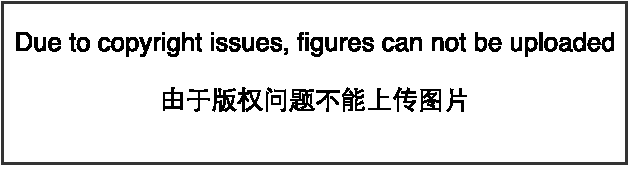
\includegraphics{figure.pdf}}
\else
\centerline{\includegraphics{Chapter6/figures/example_mlp}}
\fi
\captionsetup{singlelinecheck=off}
\caption{使用两种不同样式绘制的\gls{feedforward_network}的示例。
具体来说,这是我们用来解决XOR问题的\gls{feedforward_network}。
它有单个\gls{hidden_layer},包含两个单元。
\emph{(左)}在这种样式中,我们将每个单元绘制为图中的一个节点。
这种风格是清楚而明确的,但对于比这个例子更大的网络,它可能会消耗太多的空间。
\emph{(右)}在这种样式中,我们将表示每一层激活的整个向量绘制为图中的一个节点。
这种样式更加紧凑。
有时,我们对图中的边使用参数名进行注释,这些参数是用来描述两层之间的关系的。
这里,我们用矩阵$\bm{W}$描述从$\bm{x}$到$\bm{h}$的映射,用向量$\bm{w}$描述从$\bm{h}$到$y$的映射。
当标记这种图时,我们通常省略与每个层相关联的截距参数。}
\label{fig:chap6_example_mlp}
\end{figure}


$f^{(1)}$应该是哪种函数?线性模型到目前为止都表现不错,让$f^{(1)}$也是线性的似乎很有诱惑力。
不幸的是,如果$f^{(1)}$是线性的,那么\gls{feedforward_network}作为一个整体对于输入仍然是线性的。
暂时忽略截距项,假设$f^{(1)}(\bm{x})= \bm{W}^\top \bm{x}$并且$f^{(2)}(\bm{h})=\bm{h}^\top \bm{w}$,那么$f(\bm{x}) = \bm{w}^\top\bm{W}^\top \bm{x}$。
我们可以将这个函数重新表示成$f(\bm{x}) = \bm{x}^\top\bm{w}'$其中$\bm{w}' = \bm{W}\bm{w}$。

% -- 167 --

显然,我们必须用非线性函数来描述这些特征。
大多数神经网络通过仿射变换之后紧跟着一个被称为激活函数的固定非线性函数来实现这个目标,其中仿射变换由学得的参数控制。
我们这里使用这种策略,定义$\bm{h}=g(\bm{W}^\top \bm{x}+\bm{c})$,其中$\bm{W}$是线性变换的权重矩阵,$\bm{c}$是偏置。
先前,为了描述线性回归模型,我们使用权重向量和一个标量的偏置参数来描述从输入向量到输出标量的仿射变换。
现在,因为我们描述的是向量$\bm{x}$到向量$\bm{h}$的仿射变换,所以我们需要一整个向量的偏置参数。
激活函数$g$通常选择对每个元素分别起作用的函数,有$h_i =g(\bm{x}^\top \bm{W}_{:, i} + c_i)$。
在现代神经网络中,默认的推荐是使用由激活函数$g(z)=\max\{0, z\}$定义的\firstgls{ReLU}或者称为\glssymbol{ReLU}\citep{Jarrett-ICCV2009-small,Nair-2010-small,Glorot+al-AI-2011-small},如图\ref{fig:chap6_relu_color}所示。
% fig 6.3
\begin{figure}[!htb]
\ifOpenSource
\centerline{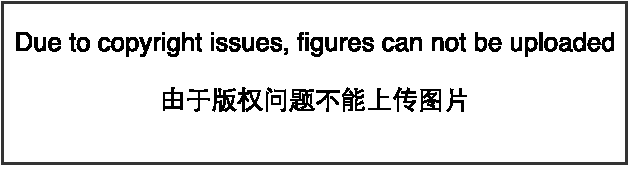
\includegraphics{figure.pdf}}
\else
\centerline{\includegraphics{Chapter6/figures/relu_color}}
\fi
\caption{\gls{rectified_linear}激活函数。
该激活函数是被推荐用于大多数\gls{feedforward_neural_network}的默认激活函数。
将此函数用于线性变换的输出将产生非线性变换。 然而,函数仍然非常接近线性,在这种意义上它是具有两个线性部分的分段线性函数。
由于\gls{ReLU}几乎是线性的,因此它们保留了许多使得线性模型易于使用基于梯度的方法进行优化的属性。 它们还保留了许多使得线性模型能够\gls{generalization}良好的属性。 计算机科学的一个公共原则是,我们可以从最小的组件构建复杂的系统。
就像图灵机的内存只需要能够存储0或1的状态,我们可以从\gls{rectified_linear}函数构建一个\gls{universal_function_approximator}。}
\label{fig:chap6_relu_color}
\end{figure}


我们现在可以指明我们的整个网络是
\begin{equation}
f(\bm{x}; \bm{W}, \bm{c}, \bm{w}, b) = \bm{w}^\top \max\{ 0, \bm{W}^\top \bm{x} + \bm{c} \} +b.
\end{equation}

% -- 168 --

% -- 169 --

我们现在可以给出XOR问题的一个解。
令
\begin{align}
\bm{W} &= \begin{bmatrix}
1 & 1\\
1 & 1
\end{bmatrix},\\
\bm{c} &= \begin{bmatrix}
0\\
-1
\end{bmatrix},\\
\bm{w} &= \begin{bmatrix}
1\\
-2
\end{bmatrix},
\end{align}
以及$b=0$。

我们现在可以了解这个模型如何处理一批输入。
令$\bm{X}$表示设计矩阵,它包含二进制输入空间中全部的四个点,每个样例占一行,那么矩阵表示为:
\begin{equation} 
\bm{X} = \begin{bmatrix}
0 & 0\\
0 & 1\\ 
1 & 0\\ 
1 & 1
\end{bmatrix}. 
\end{equation} 
神经网络的第一步是将输入矩阵乘以第一层的权重矩阵: 
\begin{equation}
\bm{X}\bm{W} = \begin{bmatrix} 
0 & 0\\ 
1 & 1\\ 
1 & 1\\ 
2 & 2 
\end{bmatrix}.
\end{equation} 
然后,我们加上偏置向量$\bm{c}$,得到 
\begin{equation} 
\begin{bmatrix} 
0 & -1\\
1 & 0\\ 
1 & 0\\ 
2 & 1 
\end{bmatrix}. 
\end{equation}
在这个空间中,所有的样例都处在一条斜率为1的直线上。
当我们沿着这条直线移动时,输出需要从0升到1,然后再降回0。
线性模型不能实现这样一种函数。
为了用$\bm{h}$对每个样例求值,我们使用\gls{rectified_linear_transformation}: 
\begin{equation}
\begin{bmatrix} 
0 & 0\\ 
1 & 0\\ 
1 & 0\\ 
2 & 1 
\end{bmatrix}. 
\end{equation}

% -- 170 --

这个变换改变了样例间的关系。它们不再处于同一条直线上了。
如图\ref{fig:chap6_relu_color}所示,它们现在处在一个可以用线性模型解决的空间上。

我们最后乘以一个权重向量$\bm{w}$:
\begin{equation}
\begin{bmatrix}
0\\
1\\
1\\
0
\end{bmatrix}.
\end{equation}
神经网络对这一批次中的每个样例都给出了正确的结果。

在这个例子中,我们简单地指明了答案,然后说明它得到的误差为零。
在实际情况中,可能会有数十亿的模型参数以及数十亿的训练样本,所以不能像我们这里做的那样进行简单地猜解。
与之相对的,基于梯度的优化算法可以找到一些参数使得产生的误差非常小。
我们这里给出的XOR问题的解处在损失函数的全局最小点,所以梯度下降算法可以收敛到这一点。
梯度下降算法还可以找到XOR问题一些其他的等价解。
梯度下降算法的收敛点取决于参数的初始值。
在实践中,梯度下降通常不会找到像我们这里给出的那种干净的、容易理解的、整数值的解。

\section{基于梯度的学习}
\label{sec:gradient_based_learning}

设计和训练神经网络与使用梯度下降训练其他任何机器学习模型并没有太大不同。
在\ref{sec:building_a_machine_learning_algorithm}节中,我们描述了如何通过指明一个优化过程、代价函数和一个模型族来构建一个机器学习算法。

我们到目前为止看到的线性模型和神经网络的最大区别,在于神经网络的非线性导致大多数我们感兴趣的损失函数都成为了非凸的。
这意味着神经网络的训练通常使用的迭代的、基于梯度的优化,仅仅使得代价函数达到一个非常小的值;而不是像用于训练线性回归模型的线性方程求解器,或者用于训练\gls{logistic_regression}或\glssymbol{SVM}的凸优化算法那样保证全局收敛。
凸优化从任何一种初始参数出发都会收敛(理论上如此——在实践中也很鲁棒但可能会遇到数值问题)。
用于非凸损失函数的随机梯度下降没有这种收敛性保证,并且对参数的初始值很敏感。
对于\gls{feedforward_neural_network},将所有的权重值初始化为小随机数是很重要的。
偏置可以初始化为零或者小的正值。
这种用于训练\gls{feedforward_neural_network}以及几乎所有深度模型的迭代的基于梯度的优化算法会在第\ref{chap:optimization_for_training_deep_models}章详细介绍,参数初始化会在\ref{sec:parameter_initialization_strategies}节中具体说明。
就目前而言,只需要懂得,训练算法几乎总是基于使用梯度来使得代价函数下降的各种方法即可。
一些特别的算法是对梯度下降思想的改进和提纯,在\ref{sec:gradient_based_optimization}节中介绍,还有一些更特别的,大多数是对随机梯度下降算法的改进,在\ref{sec:stochastic_gradient_descent_chap5}节中介绍。

% -- 171 --

我们当然也可以用梯度下降来训练诸如线性回归和\gls{SVM}之类的模型,并且事实上当训练集相当大时这是很常用的。
从这点来看,训练神经网络和训练其他任何模型并没有太大区别。
计算梯度对于神经网络会略微复杂一些,但仍然可以很高效而精确地实现。
\ref{sec:back_propagation_and_other_differentiation_algorithms}节将会介绍如何用\gls{BP}算法以及它的现代扩展算法来求得梯度。

和其他的机器学习模型一样,为了使用基于梯度的学习方法我们必须选择一个代价函数,并且我们必须选择如何表示模型的输出。
现在,我们重温这些设计上的考虑,并且特别强调神经网络的情景。

\subsection{代价函数}
\label{sec:cost_functions}

深度神经网络设计中的一个重要方面是代价函数的选择。
幸运的是,神经网络的代价函数或多或少是和其他的参数模型例如线性模型的代价函数相同的。

在大多数情况下, 我们的参数模型定义了一个分布$p(\bm{y}\mid\bm{x};\bm{\theta})$并且我们简单地使用最大似然原理。
这意味着我们使用训练数据和模型预测间的\gls{cross_entropy}作为代价函数。

有时,我们使用一个更简单的方法,不是预测$\bm{y}$的完整概率分布,而是仅仅预测在给定$\bm{x}$的条件下$\bm{y}$的某种统计量。
某些专门的损失函数允许我们来训练这些估计量的预测器。

用于训练神经网络的完整的代价函数,通常在我们这里描述的基本代价函数的基础上结合一个正则项。
我们已经在\ref{sec:regularization}节中看到正则化应用到线性模型中的一些简单的例子。
用于线性模型的权重衰减方法也直接适用于深度神经网络,而且是最流行的正则化策略之一。
用于神经网络的更高级的正则化策略会在第\ref{chap:regularization_for_deep_learning}章中讨论。

% -- 172 --

\subsubsection{用最大似然学习条件分布}
\label{sec:learning_conditional_distributions_with_maximum_likelihood}

大多数现代的神经网络使用最大似然来训练。
这意味着代价函数就是负的对数似然,它与训练数据和模型分布间的\gls{cross_entropy}等价。
这个代价函数表示为
\begin{equation}
J(\bm{\theta}) = -\SetE_{\mathbf{x}, \mathbf{y} \sim \hat{p}_\text{data}} \log p_\text{model} (\bm{y} \mid \bm{x}).
\end{equation}

代价函数的具体形式随着模型而改变,取决于$\log p_\text{model}$的具体形式。
上述方程的展开形式通常会有一些项不依赖于模型的参数,我们可以舍去。
例如,正如我们在\ref{sec:the_task_t}节中看到的,如果$p_\text{model}(\bm{y}\mid\bm{x}) = \CalN(\bm{y};f(\bm{x};\bm{\theta}), \bm{I})$,那么我们恢复\gls{mean_squared_error}代价,
\begin{equation}
J(\theta) = \frac{1}{2} \SetE_{\RVx, \RVy \sim  \hat{p}_\text{data}} || \bm{y} - f(\bm{x}; \bm{\theta}) ||^2 + \text{const},
\end{equation}
至少系数$\frac{1}{2}$和常数项不依赖于$\bm{\theta}$。
舍弃的常数是基于\gls{gaussian_distribution}的方差,在这种情况下我们选择不把它参数化。
先前,我们看到了对输出分布的最大似然估计和对线性模型\gls{mean_squared_error}的最小化之间的等价性,但事实上,这种等价性并不要求$f(\bm{x}; \bm{\theta})$用于预测\gls{gaussian_distribution}的均值。

使用最大似然来导出代价函数的方法的一个优势是,它减轻了为每个模型设计代价函数的负担。
明确一个模型$p(\bm{y}\mid\bm{x})$则自动地确定了一个代价函数$\log p(\bm{y}\mid\bm{x})$。

贯穿神经网络设计的一个反复出现的主题是代价函数的梯度必须足够的大和具有足够的预测性,来为学习算法提供一个好的指引。
饱和(变得非常平)的函数破坏了这一目标,因为它们把梯度变得非常小。
这在很多情况下都会发生,因为用于产生\gls{hidden_unit}或者输出单元的输出的激活函数会饱和。
负的对数似然帮助我们在很多模型中避免这个问题。
很多输出单元都会包含一个指数函数,这在它的变量取绝对值非常大的负值时会造成饱和。
负对数似然代价函数中的对数函数消除了某些输出单元中的指数效果。
我们将会在\ref{sec:output_units}节中讨论代价函数和输出单元的选择间的交互关系。

% -- 173 --

用于实现最大似然估计的\gls{cross_entropy}代价函数有一个不同寻常的特性,那就是当它被应用于实践中经常遇到的模型时,它通常没有最小值。
对于离散型输出变量,大多数模型以一种特殊的形式来参数化,即它们不能表示概率零和一,但是可以无限接近。
\gls{logistic_regression}是其中一个例子。
对于实值的输出变量,如果模型可以控制输出分布的密度(例如,通过学习\gls{gaussian_output_distribution}的方差参数),那么它可能对正确的训练集输出赋予极其高的密度,这将导致\gls{cross_entropy}趋向负无穷。
第\ref{chap:regularization_for_deep_learning}章中描述的正则化技术提供了一些不同的方法来修正学习问题,所以模型不会通过这种方式来获得无限制的收益。

\subsubsection{学习条件统计量}
\label{sec:learning_conditional_statistics}

有时我们并不是想学习一个完整的概率分布$p(\bm{y}\mid\bm{x}; \bm{\theta})$,而仅仅是想学习在给定$\bm{x}$时$\bm{y}$的某个条件统计量。

例如,我们可能有一个预测器$f(\bm{x}; \bm{\theta})$,我们想用它来预测$\bm{y}$的均值。
如果我们使用一个足够强大的神经网络,我们可以认为这个神经网络能够表示一大类函数中的任何一个函数$f$,这个类仅仅被一些特征所限制,例如连续性和有界,而不是具有特殊的参数形式。
从这个角度来看,我们可以把代价函数看作是一个\firstgls{functional}而不仅仅是一个函数。
泛函是函数到实数的映射。我们因此可以将学习看作是选择一个函数而不仅仅是选择一组参数。
我们可以设计代价泛函在我们想要的某些特殊函数处取得最小值。
例如,我们可以设计一个代价泛函,使它的最小值处于一个特殊的函数上,这个函数将$\bm{x}$映射到给定$\bm{x}$时$\bm{y}$的期望值。
对函数求解优化问题需要用到\firstgls{calculus_of_variations}这个数学工具,我们将在\ref{sec:calculus_of_variations}节中讨论。
理解\gls{calculus_of_variations}对于理解本章的内容不是必要的。
目前,只需要知道\gls{calculus_of_variations}可以被用来导出下面的两个结果。

% -- 174 --

我们使用\gls{calculus_of_variations}导出的第一个结果是解优化问题
\begin{equation}
f^* = \underset{f}{\argmin}  \ \SetE_{\RVx, \RVy \sim  p_\text{data}} ||\bm{y}-f(\bm{x})||^2
\end{equation}
得到
\begin{equation}
f^*(\bm{x}) = \SetE_{\RVy\sim p_\text{data}(\bm{y}|\bm{x})} [\bm{y}],
\end{equation}
要求这个函数处在我们要优化的类里。
换句话说,如果我们能够用无穷多的、来源于真实的数据生成分布的样例进行训练,最小化\gls{mean_squared_error}代价函数将得到一个函数,它可以用来对每个$\bm{x}$的值预测出$\bm{y}$的均值。

不同的代价函数给出不同的统计量。
第二个使用\gls{calculus_of_variations}得到的结果是
\begin{equation}
f^* = \underset{f}{\argmin} \ \SetE_{\RVx, \RVy \sim  p_\text{data}} ||\bm{y} - f(\bm{x})||_1
\end{equation}
将得到一个函数可以对每个$\bm{x}$预测$\bm{y}$取值的\emph{中位数},只要这个函数在我们要优化的函数族里。
这个代价函数通常被称为\firstgls{mean_absolute_error}。

可惜的是,\gls{mean_squared_error}和\gls{mean_absolute_error}在使用基于梯度的优化方法时往往成效不佳。
一些饱和的输出单元当结合这些代价函数时会产生非常小的梯度。
这就是为什么\gls{cross_entropy}代价函数比\gls{mean_squared_error}或者\gls{mean_absolute_error}更受欢迎的原因之一了,即使是在没必要估计整个$p(\bm{y}\mid\bm{x})$分布时。


\subsection{输出单元}
\label{sec:output_units}

代价函数的选择与输出单元的选择紧密相关。
大多数时候,我们简单地使用数据分布和模型分布间的\gls{cross_entropy}。
选择怎样表示输出决定了\gls{cross_entropy}函数的形式。

任何可用作输出的神经网络单元,也可以被用作\gls{hidden_unit}。
这里,我们着重讨论将这些单元用作模型输出时的情况,不过原则上它们也可以在内部使用。
我们将在\ref{sec:hidden_units}节中重温这些单元并且给出当它们被用作\gls{hidden_unit}时一些额外的细节。

在本节中,我们假设\gls{feedforward_network}提供了一组定义为$\bm{h}=f(\bm{x};\bm{\theta})$的隐藏特征。
输出层的作用是随后对这些特征进行一些额外的变换来完成整个网络必须完成的任务。

% -- 175 --

\subsubsection{用于\glsentrytext{gaussian_output_distribution}的线性单元}
\label{sec:linear_units_for_gaussian_output_distributions}

一种简单的输出单元是基于仿射变换的输出单元,仿射变换不具有非线性。
这些单元往往被直接称为线性单元。

给定特征$\bm{h}$,线性输出单元层产生一个向量$\hat{\bm{y}} = \bm{W}^\top \bm{h}+\bm{b}$。

线性输出层经常被用来产生条件\gls{gaussian_distribution}的均值:
\begin{equation}
p(\bm{y}\mid\bm{x}) = \CalN(\bm{y}; \hat{\bm{y}}, \bm{I} ).
\end{equation}
最大化其对数似然此时等价于最小化\gls{mean_squared_error}。

最大似然框架也使得学习\gls{gaussian_distribution}的协方差矩阵更加容易,或更容易地使\gls{gaussian_distribution}的协方差矩阵作为输入的函数。
然而,对于所有输入,协方差矩阵都必须被限定成一个正定矩阵。
线性输出层很难满足这种限定,所以通常使用其他的输出单元来对协方差参数化。
对协方差建模的方法在\ref{sec:other_output_types}节中简要介绍。

因为线性模型不会饱和,所以它们易于采用基于梯度的优化算法,甚至可以使用其他多种优化算法。

\subsubsection{用于\glsentrytext{bernoulli_output_distribution}的\glsentrytext{sigmoid}单元}
\label{sec:sigmoid_units_for_bernoulli_output_distributions}

许多任务需要预测二值型变量$y$的值。
具有两个类的分类问题可以归结为这种形式。

此时最大似然的方法是定义$y$在$\bm{x}$条件下的\gls{bernoulli_distribution}。

\gls{bernoulli_distribution}仅需单个参数来定义。
神经网络只需要预测$P(y =1\mid\bm{x})$即可。
为了使这个数是有效的概率,它必须处在区间$[0, 1]$中。

为满足该约束条件需要一些细致的设计工作。
假设我们打算使用线性单元,并且通过阈值来限制它成为一个有效的概率:
\begin{equation}
P(y=1 \mid \bm{x}) = \max \left \{ 0, \min \{1, \bm{w}^\top \bm{h}+b \} \right \}.
\end{equation}
这的确定义了一个有效的条件概率分布,但我们无法使用梯度下降来高效地训练它。
当$\bm{w}^\top \bm{h}+b$处于单位区间外时,模型的输出对其参数的梯度都将为$\bm{0}$。
梯度为$\bm{0}$通常是有问题的,因为学习算法对于如何改善相应的参数不再具有指导意义。

% -- 176 --

相反,最好是使用一种新的方法来保证无论何时模型给出了错误的答案时,总能有一个较大的梯度。
这种方法是基于使用\gls{sigmoid}输出单元结合最大似然来实现的。

\gls{sigmoid}输出单元定义为
\begin{equation}
\hat{y} = \sigma \left (\bm{w}^\top \bm{h} + b \right ),
\end{equation}
这里$\sigma$是第\ref{sec:useful_properties_of_common_functions}节中介绍的\gls{logistic_sigmoid}函数。

我们可以认为\gls{sigmoid}输出单元具有两个部分。
首先,它使用一个线性层来计算$z=\bm{w}^\top \bm{h}+b$。
接着,它使用\gls{sigmoid}激活函数将$z$转化成概率。

我们暂时忽略对于$\bm{x}$的依赖性,只讨论如何用$z$的值来定义$y$的概率分布。
\gls{sigmoid}可以通过构造一个非归一化(和不为1)的概率分布$\tilde{P}(y)$来得到。
我们可以随后除以一个合适的常数来得到有效的概率分布。
如果我们假定非归一化的对数概率对$y$ 和$z$是线性的,可以对它取指数来得到非归一化的概率。
我们然后对它归一化,可以发现这服从\gls{bernoulli_distribution},该分布受$z$的\gls{sigmoid}变换控制:
\begin{align}
\log \tilde{P}(y) &= yz,\\
\tilde{P}(y) &= \exp(yz),\\
P(y) &= \frac{\exp(yz)}{\sum_{y' = 0}^1 \exp(y' z)},\\
P(y) &= \sigma((2y-1)z).
\end{align}
基于指数和归一化的概率分布在统计建模的文献中很常见。
用于定义这种二值型变量分布的变量$z$被称为\firstgls{logit}。

% -- 177 --

这种在对数空间里预测概率的方法可以很自然地使用最大似然学习。
因为用于最大似然的代价函数是$-\log P(y\mid\bm{x})$,代价函数中的log抵消了\gls{sigmoid}中的exp。
如果没有这个效果,\gls{sigmoid}的饱和性会阻止基于梯度的学习做出好的改进。
我们使用最大似然来学习一个由\gls{sigmoid}参数化的\gls{bernoulli_distribution},它的损失函数为
\begin{align}
J(\bm{\theta}) &= -\log P(y\mid\bm{x})\\
&= -\log \sigma ((2y-1)z)\\
&= \zeta((1-2y)z).
\end{align}

这个推导使用了\ref{sec:useful_properties_of_common_functions}节中的一些性质。
通过将损失函数写成\gls{softplus_function}的形式,我们可以看到它仅仅在$(1-2y)z$取绝对值非常大的负值时才会饱和。
因此饱和只会出现在模型已经得到正确答案时——当$y=1$且$z$取非常大的正值时,或者$y=0$且$z$取非常小的负值时。
当$z$的符号错误时,\gls{softplus_function}的变量$(1-2y)z$可以简化为$|z|$。
当$|z|$变得很大并且$z$的符号错误时,\gls{softplus_function}渐近地趋向于它的变量$|z|$。
对$z$求导则渐近地趋向于$\text{sign}(z)$,所以,对于极限情况下极度不正确的$z$,\gls{softplus_function}完全不会收缩梯度。
这个性质很有用,因为它意味着基于梯度的学习可以很快地改正错误的$z$。

当我们使用其他的损失函数,例如\gls{mean_squared_error}之类的,损失函数会在$\sigma(z)$饱和时饱和。
\gls{sigmoid}激活函数在$z$取非常小的负值时会饱和到0,当$z$取非常大的正值时会饱和到1。
这种情况一旦发生,梯度会变得非常小以至于不能用来学习,无论此时模型给出的是正确还是错误的答案。
因此,最大似然几乎总是训练\gls{sigmoid}输出单元的优选方法。

理论上,\gls{sigmoid}的对数总是确定和有限的,因为\gls{sigmoid}的返回值总是被限制在开区间$(0, 1)$上,而不是使用整个闭区间$[0, 1]$的有效概率。
在软件实现时,为了避免数值问题,最好将负的对数似然写作$z$的函数,而不是$\hat{y}=\sigma(z)$的函数。
如果\gls{sigmoid}函数下溢到零,那么之后对$\hat{y}$取对数会得到负无穷。

\subsubsection{用于
\glsentrytext{multinoulli_output_distribution}的softmax单元}
\label{sec:softmax_units_for_multinoulli_output_distributions}

任何时候当我们想要表示一个具有$n$个可能取值的离散型随机变量的分布时,我们都可以使用softmax函数。
它可以看作是\gls{sigmoid}函数的扩展,\gls{sigmoid}函数用来表示二值型变量的分布。

% -- 178 --

softmax函数最常用作分类器的输出,来表示$n$个不同类上的概率分布。
比较少见的是,softmax函数可以在模型内部使用,例如如果我们想要在某个内部变量的$n$个不同选项中进行选择。

在二值型变量的情况下,我们希望计算一个单独的数
\begin{equation}
\hat{y} = P(y=1\mid\bm{x}).
\end{equation}
因为这个数需要处在0和1之间,并且我们想要让这个数的对数可以很好地用于对数似然的基于梯度的优化,我们选择去预测另外一个数$z=\log \hat{P}(y=1\mid\bm{x})$。
对其指数化和归一化,我们就得到了一个由\gls{sigmoid}函数控制的\gls{bernoulli_distribution}。

为了推广到具有$n$个值的离散型变量的情况,我们现在需要创造一个向量$\hat{\bm{y}}$,它的每个元素是$\hat{y}_i = P(y=i\mid\bm{x})$。
我们不仅要求每个$\hat{y}_i$元素介于0和1之间,还要使得整个向量的和为1使得它表示一个有效的概率分布。
用于\gls{bernoulli_distribution}的方法同样可以推广到\gls{multinoulli_distribution}。
首先,线性层预测了非标准化的对数概率:
\begin{equation}
\bm{z} = \bm{W}^\top \bm{h}+\bm{b},
\end{equation}
其中$z_i=\log \hat{P}(y=i\mid\bm{x})$。
softmax函数然后可以对$z$指数化和归一化来获得需要的$\hat{\bm{y}}$。
最终,softmax函数的形式为
\begin{equation}
\text{softmax}(\bm{z})_i = \frac{\exp(z_i)}{\sum_j \exp(z_j)}.
\end{equation}

和\gls{logistic_sigmoid}一样,当使用最大化对数似然训练softmax来输出目标值$\RSy$时,使用指数函数工作地非常好。
这种情况下,我们想要最大化$\log P(\RSy =i; \bm{z})=\log \text{softmax}(\bm{z})_i$。
将softmax定义成指数的形式是很自然的因为对数似然中的log可以抵消softmax中的exp:
\begin{equation}
\log \text{softmax}(\bm{z})_i = z_i - \log \sum_j \exp(z_j).
\label{eq:6.30}
\end{equation}

% -- 179 --

公式\ref{eq:6.30}中的第一项表示输入$z_i$总是对代价函数有直接的贡献。
因为这一项不会饱和,所以即使$z_i$对公式\ref{eq:6.30}的第二项的贡献很小,学习依然可以进行。
当最大化对数似然时,第一项鼓励$z_i$被推高,而第二项则鼓励所有的$\bm{z}$被压低。
为了对第二项$\log \sum_j \exp(z_j)$有一个直观的理解,注意到这一项可以大致近似为$\max_j z_j$。
这种近似是基于对任何明显小于$\max_j z_j$的$z_k$,$\exp(z_k)$都是不重要的。
我们能从这种近似中得到的直觉是,负对数似然代价函数总是强烈地惩罚最活跃的不正确预测。
如果正确答案已经具有了softmax的最大输入,那么$-z_i$项和$\log\sum_j \exp(z_j) \approx \max_j z_j = z_i$项将大致抵消。
这个样本对于整体训练代价贡献很小,将由其他未被正确分类的样本支配。

到目前为止我们只讨论了一个例子。
总体来说,未正则化的最大似然会驱动模型去学习一些参数,而这些参数会驱动softmax函数来预测在训练集中观察到的每个结果的比率:
\begin{equation}
\text{softmax}(\bm{z}(\bm{x}; \bm{\theta}))_i \approx \frac{\sum_{j=1}^m \bm{1}_{y^{(j)}=i, \bm{x}^{(j)} = \bm{x}}  }{ \sum_{j=1}^{m} \bm{1}_{\bm{x}^{(j)} = \bm{x}} }.
\end{equation}
因为最大似然是一致的估计量,所以只要模型族能够表示训练的分布,这就能保证发生。
在实践中,有限的模型能力和不完美的优化将意味着模型只能近似这些比率。

除了对数似然之外的许多目标函数对softmax函数不起作用。
具体来说,那些不使用对数来抵消softmax中的指数的目标函数,当指数函数的变量取非常小的负值时会造成梯度消失,从而无法学习。
特别是,平方误差对于softmax单元来说是一个很差的损失函数,即使模型做出高度可信的不正确预测,也不能训练模型改变其输出\citep{Bridle90}。
要理解为什么这些损失函数可能失败,我们需要检查softmax函数本身。

像\gls{sigmoid}一样,softmax激活函数可能会饱和。
\gls{sigmoid}函数具有单个输出,当它的输入极端负或者极端正时会饱和。
对于softmax的情况,它有多个输出值。
当输入值之间的差异变得极端时,这些输出值可能饱和。
当softmax饱和时,基于softmax的许多代价函数也饱和,除非它们能够转化饱和的激活函数。

% -- 180 --

为了说明softmax函数对于输入之间差异的响应,观察到当对所有的输入都加上一个相同常数时softmax的输出不变:
\begin{equation}
\text{softmax}(\bm{z}) = \text{softmax}(\bm{z}+c).
\end{equation}
使用这个性质,我们可以导出一个数值方法稳定的softmax函数的变体:
\begin{equation}
\text{softmax}(\bm{z}) = \text{softmax}(\bm{z}- \max_i z_i).
\end{equation}
变换后的形式允许我们在对softmax函数求值时只有很小的数值误差,即使是当$z$包含极正或者极负的数时。
观察softmax数值稳定的变体,可以看到softmax函数由它的变量偏离$\max_i z_i$的量来驱动。

当其中一个输入是最大($z_i = \max_i z_i$)并且$z_i$远大于其他的输入时,相应的输出$\text{softmax}(\bm{z})_i$会饱和到1。
当$z_i$不是最大值并且最大值非常大时,相应的输出$\text{softmax}(\bm{z})_i$也会饱和到0。
这是\gls{sigmoid}单元饱和方式的一般化,并且如果损失函数不被设计成对其进行补偿,那么也会造成类似的学习困难。

softmax函数的变量$\bm{z}$可以用两种方式产生。
最常见的是简单地使神经网络较早的层输出$\bm{z}$的每个元素,就像先前描述的使用线性层$\bm{z}={W}^\top\bm{h}+\bm{b}$。
虽然很直观,但这种方法是对分布的过度参数化。
$n$个输出总和必须为1的约束意味着只有$n-1$个参数是必要的;第$n$个概率值可以通过1减去前面$n-1$个概率来获得。
因此,我们可以强制要求$\bm{z}$的一个元素是固定的。
例如,我们可以要求$z_n=0$。
事实上,这正是\gls{sigmoid}单元所做的。
定义$P(y=1\mid\bm{x})=\sigma(z)$等价于用二维的$\bm{z}$以及$z_1=0$来定义$P(y=1\mid\bm{x})=\text{softmax}(\bm{z})_1$。
无论是$n-1$个变量还是$n$个变量的方法,都描述了相同的概率分布,但会产生不同的学习机制。
在实践中,无论是过度参数化的版本还是限制的版本都很少有差别,并且实现过度参数化的版本更为简单。

从神经科学的角度看,有趣的是认为softmax是一种在参与其中的单元之间形成竞争的方式:softmax输出总是和为1,所以一个单元的值增加必然对应着其他单元值的减少。
这与被认为存在于皮质中相邻神经元间的侧抑制类似。
在极端情况下(当最大的$a_i$和其他的在幅度上差异很大时),它变成了\firstgls{winner_take_all}的形式(其中一个输出接近1,其他的接近0)。

``softmax''的名称可能会让人产生困惑。
这个函数更接近于argmax函数而不是max函数。
``soft''这个术语来源于softmax函数是连续可微的。
``argmax''函数的结果表示为一个\gls{one_hot}向量(只有一个元素为1,其余元素都为0的向量),不是连续和可微的。
softmax函数因此提供了argmax的``软化''版本。max函数相应的软化版本是$\text{softmax}(\bm{z})^\top \bm{z}$。
可能最好是把softmax函数称为``softargmax'',但当前名称是一个根深蒂固的习惯了。

% -- 181 --

\subsubsection{其他的输出类型}
\label{sec:other_output_types}

先前描述的线性、\gls{sigmoid}和softmax输出单元是最常见的。
神经网络可以推广到我们希望的几乎任何种类的输出层。
最大似然原则为如何为几乎任何种类的输出层设计一个好的代价函数提供了指导。

一般的,如果我们定义了一个条件分布$p(\bm{y}\mid\bm{x}; \bm{\theta})$,最大似然原则建议我们使用$-\log p(\bm{y}\mid \bm{x};\bm{\theta})$作为代价函数。

一般来说,我们可以认为神经网络表示函数$f(\bm{x};\bm{\theta})$。
这个函数的输出不是对$\bm{y}$值的直接预测。
相反,$f(\bm{x};\bm{\theta})=\bm{\omega}$提供了$y$分布的参数。
我们的损失函数就可以表示成$-\log p(\RVy; \bm{\omega}(\bm{x}))$。

例如,我们想要学习在给定$\RVx$时$\RVy$的条件\gls{gaussian_distribution}的方差。
简单情况下,方差$\sigma^2$是一个常数,此时有一个解析表达式,这是因为方差的最大似然估计量仅仅是观测值$\RVy$与它们的期望值的差值的平方平均。
一种计算上更加昂贵但是不需要写特殊情况代码的方法是简单地将方差作为分布$p(\RVy\mid\bm{x})$的其中一个属性,这个分布受$\bm{\omega}=f(\bm{x};\bm{\theta})$控制。
负对数似然$-\log p(\bm{y};\bm{\omega}(\bm{x}))$将为代价函数提供一个必要的合适项来使我们的优化过程可以逐渐地学到方差。
在标准差不依赖于输入的简单情况下,我们可以在网络中创建一个直接复制到$\bm{\omega}$中的新参数。
这个新参数可以是$\sigma$本身,或者可以是表示$\sigma^2$的参数$v$,或者可以是表示$\frac{1}{\sigma^2}$的参数$\beta$,取决于我们怎样对分布参数化。
我们可能希望模型对不同的$\RVx$值预测出$\RVy$不同的方差。
这被称为\firstgls{heteroscedastic}模型。
在异方差情况下,我们简单地把方差指定为$f(\RVx;\bm{\theta})$其中一个输出值。
实现它的典型方法是使用精度而不是方差来表示\gls{gaussian_distribution},就像公式\ref{eq:3.22}所描述的。
在多维变量的情况下,最常见的是使用一个对角精度矩阵
\begin{equation}
\text{diag}(\bm{\beta}).
\end{equation}
这个公式适用于梯度下降,因为由$\bm{\beta}$参数化的\gls{gaussian_distribution}的对数似然的公式仅涉及$\beta_i$的乘法和$\log \beta_i$的加法。
乘法、加法和对数运算的梯度表现良好。
相比之下,如果我们用方差来参数化输出,我们需要用到除法。
除法函数在零附近会变得任意陡峭。
虽然大梯度可以帮助学习,但任意大的梯度通常导致不稳定。
如果我们用标准差来参数化输出,对数似然仍然会涉及除法,并且还将涉及平方。
通过平方运算的梯度可能在零附近消失,这使得学习被平方的参数变得困难。
无论我们使用的是标准差,方差还是精度,我们必须确保\gls{gaussian_distribution}的协方差矩阵是正定的。
因为精度矩阵的特征值是协方差矩阵特征值的倒数,所以这等价于确保精度矩阵是正定的。
如果我们使用对角矩阵,或者是一个常数乘以单位矩阵\footnote{译者注:这里原文是``If we use a diagonal matrix, or a scalar times the diagonal matrix...''即``如果我们使用对角矩阵,或者是一个标量乘以对角矩阵...'',但一个标量乘以对角矩阵和对角矩阵没区别,结合上下文可以看出,这里原作者误把``identity''写成了``diagonal matrix'',因此这里采用``常数乘以单位矩阵''的译法。},那么我们需要对模型输出强加的唯一条件是它的元素都为正。
如果我们假设$\bm{a}$是用于确定对角精度的模型的原始激活,那么可以用softplus 函数来获得正的精度向量:$\bm{\beta}=\bm{\zeta}(\bm{a})$。
这种相同的策略对于方差或标准差同样适用,也适用于常数乘以单位阵的情况。

% -- 182 --

学习一个比对角矩阵具有更丰富结构的协方差或者精度矩阵是很少见的。
如果协方差矩阵是满的和有条件的,那么参数化的选择就必须要保证预测的协方差矩阵是正定的。
这可以通过写成$\bm{\Sigma}(\bm{x})=\bm{B}(\bm{x})\bm{B}^\top (\bm{x})$来实现,这里$\bm{B}$是一个无约束的方阵。
如果矩阵是满秩的,那么一个实际问题是计算似然是很昂贵的,计算一个$d\times d$的矩阵的行列式或者$\bm{\Sigma}(\bm{x})$的逆(或者等价地并且更常用地,对它特征值分解或者$\bm{B}(\bm{x})$的特征值分解)需要$O(d^3)$的计算量。

% -- 183 --

我们经常想要执行多峰回归(multimodal regression),即预测条件分布$p(\bm{y}\mid\bm{x})$的实值,该条件分布对于相同的$\bm{x}$值在$\bm{y}$空间中有多个不同的峰值。
在这种情况下,高斯混合是输出的自然表示\citep{Jacobs-nc91,bishop1994mixture}。
带有将高斯混合作为其输出的神经网络通常被称为\firstgls{mixture_density_network}。
具有$n$个分量的高斯混合输出由下面的条件分布定义
\begin{equation}
p(\bm{y}\mid\bm{x}) = \sum_{i=1}^n p(\RSc = i \mid \bm{x}) \CalN(\bm{y}; \bm{\mu}^{(i)}(\bm{x}), \bm{\Sigma}^{(i)}(\bm{x})).
\end{equation}
神经网络必须有三个输出:定义$p(\RSc=i\mid\bm{x})$的向量,对所有的$i$给出$\bm{\mu}^{(i)}(\bm{x})$的矩阵,以及对所有的$i$给出$\bm{\Sigma}^{(i)}(\bm{x})$的张量。
这些输出必须满足不同的约束:
\begin{enumerate}
\item 混合组件$p(\RSc=i\mid\bm{x})$:它们由\gls{latent_variable}
\footnote{我们之所以认为$\RSc$是\gls{latent}的,是因为我们不能直接在数据中观测到它:给定输入$\RVx$和目标$\RVy$,不可能确切地知道是哪个高斯组件产生$\RVy$,但我们可以想象$\RVy$是通过选择其中一个来产生的,并且将那个未被观测到的选择作为随机变量。}
$\RSc$关联着,在$n$个不同组件上形成\gls{multinoulli_distribution}。
这个分布通常可以由$n$维向量的softmax来获得,以确保这些输出是正的并且和为1。

\item 均值$\bm{\mu}^{(i)}(\bm{x})$:它们指明了与第$i$个高斯组件相关联的中心或者均值,并且是无约束的(通常对于这些输出单元完全没有非线性)。
如果$\RVy$是个$d$维向量,那么网络必须输出一个由$n$个这种$d$维向量组成的$n\times d$ 的矩阵。
用最大似然来学习这些均值要比学习只有一个输出模式的分布的均值稍稍复杂一些。我们只想更新那个真正产生观测数据的组件的均值。
在实践中,我们并不知道是哪个组件产生了观测数据。
负对数似然表达式将每个样例对每个组件的贡献进行赋权,权重的大小由相应的组件产生这个样例的概率来决定。

\item 协方差$\bm{\Sigma}^{(i)}(\bm{x})$:它们指明了每个组件$i$的协方差矩阵。
和学习单个高斯组件时一样,我们通常使用对角矩阵来避免计算行列式。
和学习混合均值时一样,最大似然是很复杂的,它需要将每个点的部分责任分配给每个混合组件。
如果给定了混合模型的正确的负对数似然,梯度下降将自动地遵循正确的过程。
\end{enumerate}
有报道说基于梯度的优化方法对于混合条件高斯(作为神经网络的输出)可能是不可靠的,部分是因为涉及到除法(除以方差)可能是数值不稳定的(当某个方差对于特定的实例变得非常小时,会导致非常大的梯度)。
一种解决方法是\firstgls{clip_gradients}(见\ref{sec:clipping_gradients}节),另外一种是启发式梯度放缩\citep{Uria+al-ICML2014}。

% -- 184 --

高斯混合输出在语音生成模型\citep{schuster1999supervised}和物理运动\citep{Graves-arxiv2013}中特别有效。
混合密度策略为网络提供了一种方法来表示多种输出模式,并且控制输出的方差,这对于在这些实数域中获得高质量的结果是至关重要的。
混合密度网络的一个实例如图\ref{fig:chap6_mdn_color}所示。
% fig 6.4
\begin{figure}[!htb]
\ifOpenSource
\centerline{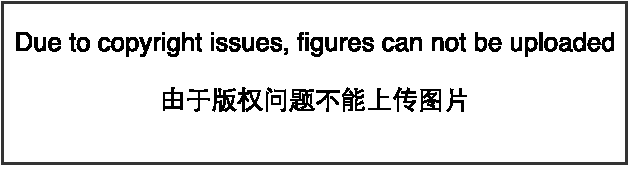
\includegraphics{figure.pdf}}
\else
\centerline{\includegraphics{Chapter6/figures/mdn_color}}
\fi
\captionsetup{singlelinecheck=off}
\caption{从具有混合密度输出层的神经网络中抽取的样本。
输入$x$从\gls{uniform_distribution}中采样,输出$y$从$p_{\text{model}}(y\mid x)$中采样。 神经网络能够学习从输入到输出分布的参数的非线性映射。 这些参数包括控制三个组件中的哪一个将产生输出的概率,以及每个组件各自的参数。
每个混合组件都是\gls{gaussian_distribution},具有预测的均值和方差。 输出分布的这些方面都能够相对输入$x$变化,并且以非线性的方式改变。}
\label{fig:chap6_mdn_color}
\end{figure}


一般的,我们可能希望继续对包含更多变量的更大的向量$\bm{y}$来建模,并在这些输出变量上施加更多更丰富的结构。
例如,我们可能希望神经网络输出字符序列形成一个句子。
在这些情况下,我们可以继续使用最大似然原理应用到我们的模型$p(\bm{y};\bm{\omega}(\bm{x}))$上,但我们用来描述$\bm{y}$的模型会变得非常复杂,超出了本章的范畴。
第\ref{chap:sequence_modeling_recurrent_and_recursive_nets}章描述了如何用循环神经网络来定义这种序列上的模型,第\ref{part:deep_learning_research}部分描述了对任意概率分布进行建模的高级技术。

\section{\glsentrytext{hidden_unit}}
\label{sec:hidden_units}

到目前为止我们集中讨论了神经网络的设计选择,这对于使用基于梯度的优化方法来训练的大多数参数化机器学习模型都是通用的。
现在我们转向一个\gls{feedforward_neural_network}独有的问题:该如何选择\gls{hidden_unit}的类型,这些\gls{hidden_unit}用在模型的\gls{hidden_layer}中。

% -- 185 --

\gls{hidden_unit}的设计是一个非常活跃的研究领域,并且还没有许多明确的指导性理论原则。

\gls{ReLU}是\gls{hidden_unit}极好的默认选择。
许多其他类型的\gls{hidden_unit}也是可用的。
决定何时使用哪种类型的\gls{hidden_unit}是困难的事(尽管\gls{ReLU}通常是一个可接受的选择)。
我们这里描述对于每种\gls{hidden_unit}的一些基本直觉。
这些直觉可以用来建议我们何时来尝试一些单元。
通常不可能预先预测出哪种\gls{hidden_unit}工作得最好。
设计过程充满了试验和错误,先直觉认为某种\gls{hidden_unit}可能表现良好,然后用它组成神经网络进行训练,最后用校验集来评估它的性能。

这里列出的一些\gls{hidden_unit}可能并不是在所有的输入点上都是可微的。
例如,\gls{ReLU} $g(z)=\max\{0, z\}$在$z=0$处不可微。
这似乎使得$g$对于基于梯度的学习算法无效。
在实践中,梯度下降对这些机器学习模型仍然表现得足够好。
部分原因是神经网络训练算法通常不会达到代价函数的局部最小值,而是仅仅显著地减小它的值,如图\ref{fig:chap4_approx_opt_color}所示。
这些想法会在第\ref{chap:optimization_for_training_deep_models}章中进一步描述。
因为我们不再期望训练能够实际到达梯度为$\bm{0}$的点,所以代价函数的最小值对应于梯度未定义的点是可以接受的。
不可微的\gls{hidden_unit}通常只在少数点上不可微。
一般来说,函数$g(z)$具有左导数和右导数,左导数定义为紧邻在$z$左边的函数的斜率,右导数定义为紧邻在$z$右边的函数的斜率。
只有当函数在$z$处的左导数和右导数都有定义并且相等时,函数在$z$点处才是可微的。
神经网络中用到的函数通常对左导数和右导数都有定义。
在$g(z)=\max\{0,z\}$的情况下,在$z=0$处的左导数是0,右导数是1。
神经网络训练的软件实现通常返回左导数或右导数的其中一个,而不是报告导数未定义或产生一个错误。
这可以通过观察到在数字计算机上基于梯度的优化总是会受到数值误差的影响来启发式地给出理由。
当一个函数被要求计算$g(0)$时,底层值真正为0 是不太可能的。
相对的,它可能是被舍入为0的一个小量$\epsilon$。
在某些情况下,理论上更好的理由可以使用,但这些通常对神经网络训练并不适用。
重要的是,在实践中,我们可以放心地忽略下面描述的\gls{hidden_unit}激活函数的不可微性。

% -- 186 --

除非另有说明,大多数的\gls{hidden_unit}都可以描述为接受输入向量$\bm{x}$,计算仿射变换$\bm{z}=\bm{W}^\top \bm{x}+\bm{b}$,然后使用一个作用于每个元素的非线性函数$g(\bm{z})$。
大多数\gls{hidden_unit}的区别仅仅在于激活函数$g(\bm{z})$的形式。

\subsection{\glsentrytext{ReLU}及其扩展}
\label{sec:rectified_linear_units_and_their_generalizations}

\gls{ReLU}使用激活函数$g(z)=\max\{0, z\}$。

\gls{ReLU}易于优化,因为它们和线性单元非常类似。
线性单元和\gls{ReLU}的唯一区别在于\gls{ReLU}在其一半的定义域上输出为零。
这使得只要\gls{ReLU}处于激活状态它的导数都能保持较大。
它的梯度不仅大而且一致。
整流操作的二阶导数几乎处处为0,并且在\gls{ReLU}处于激活状态时它的一阶导数处处为1。
这意味着它的梯度方向对于学习来说更加有用,相比于引入二阶效应的激活函数。

\gls{ReLU}通常用于仿射变换之上:
\begin{equation}
\bm{h} = g(\bm{W}^\top \bm{x} + \bm{b}).
\end{equation}
当初始化仿射变换的参数时,可以将$\bm{b}$的所有元素设置成一个小的正值,例如0.1。
这使得\gls{ReLU}很可能初始时就对训练集中的大多数输入呈现激活状态,并且允许导数通过。

有很多\gls{ReLU}的扩展存在。
大多数这些扩展的表现比得上\gls{ReLU},并且偶尔表现得更好。

\gls{ReLU}的一个缺陷是它们不能通过基于梯度的方法学习那些使它们激活为零的样例。
\gls{ReLU}的各种扩展保证了它们能在各个位置都接收到梯度。

\gls{ReLU}的三个扩展基于当$z_i<0$时使用一个非零的斜率$\alpha_i$:$h_i =g(\bm{z}, \bm{\alpha})_i = \max(0, z_i) + \alpha_i \min(0, z_i)$。
\firstgls{absolute_value_rectification}固定$\alpha_i=-1$来得到$g(z)=|z|$。
它用于图像中的对象识别\citep{Jarrett-ICCV2009},其中寻找在输入照明极性反转下不变的特征是有意义的。
\gls{ReLU}的其他扩展更广泛地适用。
\firstgls{leaky_ReLU}\citep{Maas-et-al-ICML2013}将$\alpha_i$固定成一个类似0.01的小值,\firstgls{PReLU}或者\textbf{\glssymbol{PReLU}}将$\alpha_i$作为学习的参数\citep{He-et-al-arxiv2015}。

% -- 187 --

\firstgls{maxout_unit}\citep{Goodfellow_maxout_2013}进一步扩展了\gls{ReLU}。
并不是使用作用于每个元素的函数$g(z)$,\gls{maxout_unit}将$\bm{z}$划分为具有$k$个值的组。
每个\gls{maxout_unit}然后输出其中一组的最大元素:
\begin{equation}
g(\bm{z})_i = \underset{j\in \SetG^{(i)}}{\max} z_j
\end{equation}
这里$\SetG^{(i)}$是组$i$的输入指标集$\{(i-1)k+1, \ldots, ik\}$。
这提供了一种方法来学习对输入$\bm{x}$空间中多个方向响应的分段线性函数。

\gls{maxout_unit}可以学习具有多达$k$段的分段线性的凸函数。
\gls{maxout_unit}因此可以视为\textbf{学习激活函数}本身而不仅仅是单元之间的关系。
使用足够大的$k$,\gls{maxout_unit}可以以任意的逼真度来近似任何凸函数。
特别地,具有每组两块的maxout层可以学习实现和传统层相同的输入$\bm{x}$的函数,包括\gls{rectified_linear}激活函数、\gls{absolute_value_rectification}、\gls{leaky_ReLU} 或\gls{PReLU}、或者可以学习实现与这些都不同的函数。
maxout层的参数化当然也将与这些层不同,所以即使是maxout学习去实现和其他种类的层相同的$\bm{x}$的函数这种情况下,学习的机理也是不一样的。

每个\gls{maxout_unit}现在由$k$个权重向量来参数化,而不仅仅是一个,所以\gls{maxout_unit}通常比\gls{ReLU}需要更多的正则化。
如果训练集很大并且每个单元分得的块数保持很低的话,它们可以在没有正则化的情况下正常工作\citep{cai2013deep}。

\gls{maxout_unit}还有一些其他的优点。
在某些情况下,需要更少的参数可以获得一些统计和计算上的优点。
具体来说,如果由$n$个不同的线性过滤器描述的特征可以在不损失信息的情况下,用每一组$k$个特征的最大值来概括的话,那么下一层可以获得$k$倍更少的权重数 。

因为每个单元由多个过滤器驱动,\gls{maxout_unit}具有一些冗余来帮助它们抵抗一种被称为\firstgls{catastrophic_forgetting}的现象,这个现象是说神经网络忘记了如何执行它们过去训练的任务\citep{Goodfellow+al-ICLR2014-small}。

\gls{ReLU}和它们的这些扩展都是基于一个原则,那就是如果它们的行为更接近线性,那么模型更容易优化。
使用线性行为更容易优化的一般性原则同样也适用在除了深度线性网络以外的内容。
循环网络可以从序列中学习并产生状态和输出的序列。
当训练它们时,需要通过一些时间步长来传播信息,当其中包含一些线性计算(具有大小接近1的某些方向导数)时,这会更容易。
作为性能最好的循环网络结构之一,LSTM通过求和来在时间上传播信息,这是一种特别直观的线性激活。
它将在\ref{sec:the_long_short_term_memory_and_other_gated_rnns}节中进一步讨论。

% -- 188 --

\subsection{\gls{logistic_sigmoid}与双曲正切函数}
\label{sec:logistic_sigmoid_and_hyperbolic_tangent}

在引入\gls{ReLU}之前,大多数神经网络使用\gls{logistic_sigmoid}激活函数
\begin{equation}
g(z) = \sigma(z)
\end{equation}
或者是双曲正切激活函数
\begin{equation}
g(z) = \text{tanh}(z).
\end{equation}
这些激活函数紧密相关,因为$\text{tanh}(z)=2\sigma(2z)-1$。

我们已经看过\gls{sigmoid}单元作为输出单元用来预测二值型变量取值为1的概率。
与分段线性单元不同,\gls{sigmoid}单元在其大部分定义域内都饱和——当$z$取绝对值很大的正值时,它们饱和到一个高值,当$z$取绝对值很大的负值时,它们饱和到一个低值,并且仅仅当$z$接近0时它们才对输入强烈敏感。
\gls{sigmoid}单元的广泛饱和性会使得基于梯度的学习变得非常困难。
因为这个原因,现在不鼓励将它们用作前馈网络中的\gls{hidden_unit}。
它们作为输出单元可以与基于梯度的学习相兼容,如果使用了一个合适的代价函数来抵消\gls{sigmoid}的饱和性的话。

当必须要使用\gls{sigmoid}激活函数时,双曲正切激活函数通常要比\gls{logistic_sigmoid}函数表现更好。
在$\text{tanh}(0)=0$而$\sigma(0)=\frac{1}{2}$的意义上,它更像是单位函数。
因为$\text{tanh}$在0附近与单位函数类似,训练深层神经网络$\hat{y}=\bm{w}^\top \text{tanh}(\bm{U}^\top \text{tanh}(\bm{V}^\top \bm{x}))$类似于训练一个线性模型$\hat{y}= \bm{w}^\top \bm{U}^\top \bm{V}^\top \bm{x}$,只要网络的激活能够被保持地很小。
这使得训练$\text{tanh}$网络更加容易。

% -- 189 --

\gls{sigmoid}激活函数在除了\gls{feedforward_network}以外的配置中更为常见。
循环网络、许多概率模型以及一些\gls{AE}有一些额外的要求使得它们不能使用分段线性激活函数,并且使得\gls{sigmoid}单元更具有吸引力,尽管它存在饱和性的问题。

\subsection{其他\gls{hidden_unit}}
\label{sec:other_hidden_units}

也存在许多其他种类的\gls{hidden_unit},但它们并不常用。

一般来说,很多种类的可微函数都表现得很好。
许多未发布的激活函数与流行的激活函数表现得一样好。
为了提供一个具体的例子,作者在MNIST数据集上使用$\bm{h}=\cos(\bm{W}\bm{x}+\bm{b})$测试了一个\gls{feedforward_network},并获得了小于1\%的误差率,这可以与更为传统的激活函数获得的结果相媲美。
在新技术的研究和开发期间,通常会测试许多不同的激活函数,并且会发现许多标准方法的变体表现非常好。
这意味着,通常新的\gls{hidden_unit}类型只有在被明确证明能够提供显著改进时才会被发布。
新的\gls{hidden_unit}类型如果与已有的\gls{hidden_unit}表现大致相当的话,那么它们是非常常见的,不会引起别人的兴趣。

想要列出文献中出现的所有\gls{hidden_unit}类型是不切实际的。
我们只对一些特别有用和独特的类型进行强调。

其中一种是完全没有激活函数$g(z)$。
也可以认为这是使用单位函数作为激活函数。
我们已经看过线性单元可以用作神经网络的输出。
它也可以用作\gls{hidden_unit}。
如果神经网络的每一层都仅由线性变换组成,那么网络作为一个整体也将是线性的。
然而,神经网络的一些层是纯线性也是可以接受的。
考虑具有$n$个输入和$p$个输出的神经网络层$\bm{h}=g(\bm{W}^\top \bm{x}+\bm{b})$。
我们可以用两层来代替它,一层使用权重矩阵$\bm{U}$,另一层使用权重矩阵$\bm{V}$。
如果第一层没有激活函数,那么我们对基于$\bm{W}$的原始层的权重矩阵进行因式分解。
分解方法是计算$\bm{h}=g(\bm{V}^\top \bm{U}^\top \bm{x}+\bm{b})$。
如果$U$产生了$q$个输出,那么$\bm{U}$和$V$一起仅包含$(n+p)q$个参数,而$\bm{W}$包含$np$个参数。
如果$q$很小,这可以在很大程度上节省参数。
这是以将线性变换约束为低秩的代价来实现的,但这些低秩关系往往是足够的。
线性\gls{hidden_unit}因此提供了一种减少网络中参数数量的有效方法。

% -- 190 --


softmax单元是另外一种经常用作输出的单元(如第\ref{sec:softmax_units_for_multinoulli_output_distributions}节中所描述的),但有时也可以用作\gls{hidden_unit}。
softmax单元很自然地表示具有$k$个可能值的离散型随机变量的概率分布,所以它们可以用作一种开关。
这些类型的\gls{hidden_unit}通常仅用于明确地学习操作内存的高级结构中,将在\ref{sec:explicit_memory}节中描述。

其他一些常见的\gls{hidden_unit}类型包括:
\begin{itemize}
\item \firstall{RBF}:$h_i = \exp \left (-\frac{1}{\sigma_i^2}|| \bm{W}_{:,i}-\bm{x}||^2 \right )$。
这个函数在$\bm{x}$接近模板$\bm{W}_{:,i}$时更加活跃。
因为它对大部分$\bm{x}$都饱和到0,因此很难优化。

\item \textbf{\gls{softplus}}函数:$g(a)=\zeta(a)=\log(1+e^a)$。
这是\gls{ReLU}的平滑版本,由\cite{Dugas01}引入用于函数近似,由\cite{Nair-2010-small}引入用于无向概率模型的条件分布。
\cite{Glorot+al-AI-2011-small}比较了softplus和\gls{ReLU},发现后者的结果更好。
通常不鼓励使用\gls{softplus_function}。
softplus表明\gls{hidden_unit}类型的性能可能是非常反直觉的——因为它处处可导或者因为它不完全饱和,人们可能希望它具有优于\gls{ReLU}的点,但根据经验来看,它并没有。

\item \firstgls{hard_tanh}:它的形状和$\text{tanh}$以及\gls{ReLU}类似,但是不同于后者,它是有界的,$g(a)=\max(-1, \min(1,a))$。
它由\cite{Collobert04}引入。
\end{itemize}

\gls{hidden_unit}的设计仍然是一个活跃的研究领域,许多有用的\gls{hidden_unit}类型仍有待发现。

\section{结构设计}
\label{sec:architecture_design}

神经网络设计的另一个关键点是确定它的结构。
\firstgls{architecture}一词是指网络的整体结构:它应该具有多少单元,以及这些单元应该如何连接。

% -- 191 --

大多数神经网络被组织成称为层的单元组。
大多数神经网络结构将这些层布置成链式结构,其中每一层都是前一层的函数。
在这种结构中,第一层由下式给出:
\begin{equation}
\bm{h}^{(1)}= g^{(1)}\left ( \bm{W}^{(1)\top} \bm{x} + \bm{b}^{(1)}\right );
\end{equation}
第二层由
\begin{equation}
\bm{h}^{(2)} = g^{(2)}\left ( \bm{W}^{(2)\top}\bm{h}^{(1)}+\bm{b}^{(2)} \right );
\end{equation}
给出,以此类推。

在这些链式结构中,主要的结构考虑是选择网络的深度和每一层的宽度。
我们将会看到,即使只有一个\gls{hidden_layer}的网络也足够适应训练集。
更深层的网络通常能够对每一层使用更少的单元数和更少的参数,并且经常推广到测试集,但是通常也更难以优化。
对于一个具体的任务,理想的网络结构必须通过实验,观测在验证集上的错误来找到。

\subsection{通用近似性质和深度}
\label{sec:universal_approximation_properties_and_depth}

线性模型,通过矩阵乘法将特征映射到输出,顾名思义,仅能表示线性函数。
它具有易于训练的优点,因为当使用线性模型时,许多损失函数会导出凸优化问题。
不幸的是,我们经常想要学习非线性函数。

乍一看,我们可能认为学习非线性函数需要为我们想要学习的那种非线性专门设计一类模型族。
幸运的是,具有\gls{hidden_layer}的\gls{feedforward_network}提供了一种通用近似框架。
具体来说,\firstgls{universal_approximation_theorem}\citep{Hornik89,Cybenko89}表明,一个\gls{feedforward_neural_network}如果具有线性输出层和至少一层具有任何一种``挤压''性质的激活函数(例如\gls{logistic_sigmoid}激活函数)的\gls{hidden_layer},只要给予网络足够数量的\gls{hidden_unit},它可以以任意的精度来近似任何从一个有限维空间到另一个有限维空间的Borel可测函数。
\gls{feedforward_network}的导数也可以任意好地来近似函数的导数\citep{hornik1990universal}。
Borel可测的概念超出了本书的范畴;对于我们想要实现的目标,只需要知道定义在$\SetR^n$的有界闭集上的任意连续函数是Borel可测的,因此可以用神经网络来近似。
神经网络也可以近似从任何有限维离散空间映射到另一个的任意函数。
虽然原始定理最初以具有特殊激活函数的单元的形式来描述,这个激活函数当变量取绝对值非常大的正值和负值时都会饱和,通用近似定理也已经被证明对于更广泛类别的激活函数也是适用的,其中就包括现在常用的\gls{ReLU}\citep{Leshno-et-al-1993}。

% -- 192 --

通用近似定理意味着无论我们试图学习什么函数,我们知道一个大的MLP一定能够\textbf{表示}这个函数。
然而,我们不能保证训练算法能够\textbf{学得}这个函数。
即使MLP能够表示该函数,学习也可能因两个不同的原因而失败。
首先,用于训练的优化算法可能找不到用于期望函数的参数值。
其次,训练算法可能由于过拟合选择了错误的函数。
回忆\ref{sec:the_no_free_lunch_theorem}节中的``没有免费的午餐''定理说明了没有普遍优越的机器学习算法。
\gls{feedforward_network}提供了表示函数的通用系统,在这种意义上,给定一个函数,存在一个\gls{feedforward_network}能够近似该函数。
不存在通用的过程既能够验证训练集上的特殊样例,又能够选择一个函数来扩展到训练集上没有的点。

通用近似定理说明了存在一个足够大的网络能够达到我们所希望的任意精度,但是定理并没有说这个网络有多大。
\cite{Barron93}提供了单层网络近似一大类函数所需大小的一些界。
不幸的是,在最坏情况下,可能需要指数数量的\gls{hidden_unit}(可能一个\gls{hidden_unit}对应着一个需要区分的输入配置)。
这在二进制情况下很容易看到:向量$\bm{v}\in \{0,1\}^n$上的可能的二进制函数的数量是$2^{2^n}$并且选择一个这样的函数需要$2^n$位,这通常需要$O(2^n)$的自由度。

总之,具有单层的\gls{feedforward_network}足以表示任何函数,但是网络层可能不可实现得大并且可能无法正确地学习和\gls{generalization}。
在很多情况下,使用更深的模型能够减少表示期望函数所需的单元的数量,并且可以减少\gls{generalization}误差。

% -- 193 --

存在一些函数族能够在网络的深度大于某个值$d$时被高效地近似,而当深度被限制到小于或等于$d$时需要一个远远大于之前的模型。
在很多情况下,浅层模型所需的\gls{hidden_unit}的数量是$n$的指数级。
这个结果最初被证明是在那些不与连续可微的神经网络类似的机器学习模型中出现,但现在已经扩展到了这些模型。
第一个结果是关于逻辑门电路的\citep{Hastad86}。
后来的工作将这些结果扩展到了具有非负权重的线性阈值单元\citep{Hastad91,Hajnal-et-al-1993},然后扩展到了具有连续值激活的网络\citep{Maass-1992,Maass-et-al-1994}。
许多现代神经网络使用\gls{ReLU}。
\cite{Leshno-et-al-1993}证明带有一大类非多项式激活函数族的浅层网络,包括\gls{ReLU},具有通用的近似性质,但是这些结果并没有强调深度或效率的问题——它们仅指出足够宽的\gls{rectifier_network}能够表示任意函数。
\cite{Montufar-et-al-NIPS2014}指出一些用深度\gls{rectifier_network}表示的函数可能需要浅层网络(一个\gls{hidden_layer})指数级的\gls{hidden_unit}才能表示。
更确切的说,他们说明分段线性网络(可以通过整流非线性或\gls{maxout_unit}获得)可以表示区域的数量是网络深度的指数级的函数。%这里为什么是非线性?
图\ref{fig:chap6_space_folding}解释了带有\gls{absolute_value_rectification}的网络是如何创建函数的镜像图像的,这些函数在某些\gls{hidden_unit}的顶部计算,作用于\gls{hidden_unit}的输入。
每个\gls{hidden_unit}指定在哪里折叠输入空间,来创造镜像响应(在绝对值非线性的两侧)。
通过组合这些折叠操作,我们获得指数级的分段线性区域,他们可以概括所有种类的规则模式(例如,重复)。
% fig 6.5
\begin{figure}[!htb]
\ifOpenSource
\centerline{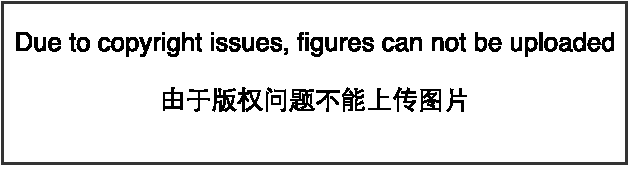
\includegraphics{figure.pdf}}
\else
\centerline{\includegraphics[width=\textwidth]{Chapter6/figures/space_folding.jpg}}
\fi
\caption{ % This is a screenshot.
关于更深的整流网络具有指数优势的一个直观的几何解释,来自\cite{Montufar-et-al-NIPS2014}。 
\emph{(左)}\gls{absolute_value_rectification}单元对其输入中的每对镜像点有相同的输出。
镜像的对称轴由单元的权重和偏置定义的超平面给出。 在该单元顶部计算的函数(绿色决策面)将是横跨该对称轴的更简单模式的一个镜像。 
\emph{(中)}该函数可以通过折叠对称轴周围的空间来得到。
\emph{(右)}另一个重复模式可以在第一个的顶部折叠(由另一个下游单元)以获得另外的对称性(现在重复四次,使用了两个\gls{hidden_layer})。 
图重置得到了\cite{Montufar-et-al-NIPS2014}的许可。}
\label{fig:chap6_space_folding}
\end{figure}


更确切的说,\cite{Montufar-et-al-NIPS2014}的主要定理指出,具有$d$个输入,深度为$l$,每个\gls{hidden_layer}有$n$个单元的深度\gls{rectifier_network}可以描述的线性区域的数量是
\begin{equation}
O \left ( {n \choose d}^{d(l-1)} n^d \right ),
\end{equation}
这意味着,是深度$l$的指数级。
在每个单元具有$k$个过滤器的maxout网络中,线性区域的数量是
\begin{equation}
O \left ( k^{(l-1)+d} \right ).
\end{equation}

% -- 194 --

当然,我们不能保证在机器学习(特别是AI)的应用中我们想要学得的函数类型享有这样的属性。

我们还可能出于统计原因来选择深度模型。
任何时候,当我们选择一个特定的机器学习算法时,我们隐含地陈述了一些先验,这些先验是关于算法应该学得什么样的函数的。
选择深度模型默许了一个非常普遍的信念,那就是我们想要学得的函数应该涉及几个更加简单的函数的组合。
这可以从表示学习的观点来解释, 我们相信学习的问题包含发现一组潜在的变化因素,它们可以根据其他更简单的潜在的变化因素来描述。
或者,我们可以将深度结构的使用解释为另一种信念,那就是我们想要学得的函数是包含多个步骤的计算机程序,其中每个步骤使用前一步骤的输出。
这些中间输出不一定是变化的因素,而是可以类似于网络用来组织其内部处理的计数器或指针。
根据经验,更深的模型似乎确实会更适用于广泛的任务\citep{Bengio-NIPS2007,Erhan2009,Bengio-2009-book,UTLC+LISA-2011-small,Ciresan-et-al-2012,Krizhevsky-2012-small,sermanet-cvpr-13,Farabet-et-al-2013,couprie-iclr-13,LISA-EmotiW2013,Goodfellow+et+al-ICLR2014a,Szegedy-et-al-arxiv2014}。
图\ref{fig:chap6_depth_color}和图\ref{fig:chap6_model_size_color}展示了一些实验结果的例子。
这表明使用深层结构确实在模型学习的函数空间上表示了一个有用的先验。
% fig 6.6
\begin{figure}[!htb]
\ifOpenSource
\centerline{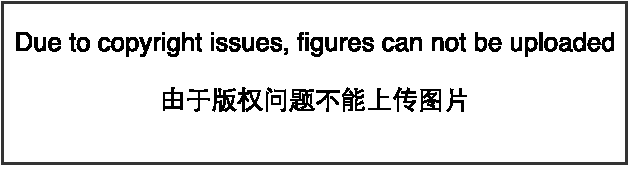
\includegraphics{figure.pdf}}
\else
\centerline{\includegraphics{Chapter6/figures/depth_color}}
\fi
\caption{深度的影响。
实验结果表明,当从地址照片转录多位数字时,更深层的网络能够更好地\gls{generalization}。
数据来自\cite{Goodfellow+et+al-ICLR2014a}。
测试集上的准确率随着深度的增加而不断增加。
图\ref{fig:chap6_model_size_color}给出了一个对照实验,它说明了对模型尺寸其他方面的增加并不能产生相同的效果。}
\label{fig:chap6_depth_color}
\end{figure}

% fig 6.7
\begin{figure}[!htb]
\ifOpenSource
\centerline{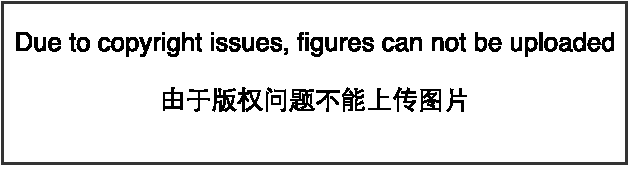
\includegraphics{figure.pdf}}
\else
\centerline{\includegraphics{Chapter6/figures/model_size_color}}
\fi
\caption{参数数量的影响。
更深的模型往往表现更好。
这不仅仅是因为模型更大。
\cite{Goodfellow+et+al-ICLR2014a}的这项实验表明,增加\gls{convolutional_network}层中参数的数量,但是不增加它们的深度,在提升测试集性能方面几乎没有效果,如此图所示。
图例标明了用于画出每条曲线的网络深度,以及曲线表示的是卷积层还是全连接层的大小变化。
我们可以观察到,在这种情况下,浅层模型在参数数量达到2000万时就过拟合,而深层模型在参数数量超过6000万时仍然表现良好。
这表明,使用深层模型表达出了对模型可以学习的函数空间的有用偏好。
具体来说,它表达了一种信念,即该函数应该由许多更简单的函数复合在一起而得到。
这可能导致学习由更简单的表示所组成的表示(例如,由边所定义的角)或者学习具有顺序依赖步骤的程序(例如,首先定位一组对象,然后分割它们,之后识别它们)。}
\label{fig:chap6_model_size_color}
\end{figure}

\subsection{其他结构上的考虑}
\label{sec:other_architectural_considerations}

到目前为止,我们都将神经网络描述成简单的层的链式结构,主要的考虑因素是网络的深度和每层的宽度。
在实践中,神经网络显示出相当的多样性。

许多神经网络结构已经被开发用于特定的任务。
用于计算机视觉的卷积神经网络的特殊结构将在第\ref{chap:convolutional_networks}章中介绍。
\gls{feedforward_network}也可以推广到用于序列处理的循环神经网络,但有它们自己的结构考虑,将在第\ref{chap:sequence_modeling_recurrent_and_recursive_nets}章中介绍。

% -- 195 --

一般的,层不需要连接在链中,尽管这是最常见的做法。
许多结构构建了一个主链,但随后又添加了额外的结构属性,例如从层$i$到层$i+2$或者更高层的跳动连接。
这些跳动连接使得梯度更容易从输出层流向更接近输入的层。

结构设计考虑的另外一个关键点是如何将层与层之间连接起来。
默认的神经网络层采用矩阵$\bm{W}$描述的线性变换,每个输入单元连接到每个输出单元。
在之后章节中的许多专用网络具有较少的连接,使得输入层中的每个单元仅连接到输出层单元的一个小子集。
这些用于减少连接数量的策略减少了参数的数量以及用于评估网络的计算量,但通常高度依赖于问题。
例如,第\ref{chap:convolutional_networks}章描述的卷积神经网络使用对于计算机视觉问题非常有效的稀疏连接的专用模式。
在这一章中,很难对通用神经网络的结构给出更多具体的建议。
随后的章节研发了一些特殊的结构策略,可以在不同的领域工作良好。

% -- 196 --

\section{\gls{BP}和其他的微分算法}
\label{sec:back_propagation_and_other_differentiation_algorithms}

当我们使用\gls{feedforward_neural_network}接收输入$\bm{x}$并产生输出$\hat{\bm{y}}$时,信息通过网络向前流动。
输入$\bm{x}$提供初始信息,然后传播到每一层的\gls{hidden_unit},最终产生输出$\hat{\bm{y}}$。
这称之为\firstgls{forward_propagation}。
在训练过程中,前向传播可以持续向前直到它产生一个标量代价函数$J(\bm{\theta})$。
\firstgls{back_propagation}算法\citep{RHW},经常简称为\textbf{\glsdesc{BP}},允许来自代价函数的信息通过网络向后流动,以便计算梯度。

% -- 197 --

计算梯度的解析表达式是很直观的,但是数值化地求解这样的表达式在计算上可能是昂贵的。
 反向传播算法使用简单和廉价的程序来实现这个目标。

反向传播这个术语经常被误解为用于多层神经网络的整个学习算法。
实际上,反向传播仅指用于计算梯度的方法,而另一种算法,例如随机梯度下降,使用该梯度来进行学习。
此外,反向传播经常被误解为仅适用于多层神经网络,但是原则上它可以计算任何函数的导数(对于一些函数,正确的响应是报告函数的导数是未定义的)。
特别地,我们会描述如何计算一个任意函数$f$的梯度$\nabla_{\bm{x}} f(\bm{x}, \bm{y})$,其中$\bm{x}$是一组变量,我们需要它们的导数,而$\bm{y}$是函数的另外一组输入变量,但我们并不需要它们的导数。
在学习算法中,我们最常需要的梯度是代价函数关于参数的梯度,即$\nabla_{\bm{\theta}} J(\bm{\theta})$。
许多机器学习任务需要计算其他导数,来作为学习过程的一部分,或者用来分析学得的模型。
反向传播算法也适用于这些任务,不局限于计算代价函数关于参数的梯度。
通过在网络中传播信息来计算导数的想法非常普遍,它还可以用于计算诸如多输出函数$f$的\gls{jacobian_matrix}的值。
我们这里描述的是最常用的情况,$f$只有单个输出。

\subsection{计算图}
\label{sec:computational_graphs}

到目前为止我们已经用相对非正式的图形语言讨论了神经网络。
为了更精确地描述反向传播算法,使用更精确的\firstgls{computational_graph}语言是很有帮助的。

将计算形式化为图形的方法有很多。

这里,我们使用图中的每一个节点来表示一个变量。
变量可以是标量、向量、矩阵、张量、或者甚至是另一类型的变量。

为了形式化我们的图形,我们还需引入\firstgls{operation}这一概念。
操作是指一个或多个变量的简单函数。
我们的图形语言伴随着一组被允许的操作。
我们可以通过将多个操作复合在一起来描述更为复杂的函数。

% -- 198 --

不失一般性,我们定义一个操作仅返回单个输出变量。
这并没有失去一般性,是因为输出变量可以有多个条目,例如向量。
反向传播的软件实现通常支持具有多个输出的操作,但是我们在描述中避免这种情况,因为它引入了对概念理解不重要的许多额外细节。

如果变量$y$是变量$x$通过一个操作计算得到的,那么我们画一条从$x$到$y$的有向边。
我们有时用操作的名称来注释输出的节点,当上下文很明确时有时也会省略这个标注。

计算图的实例可以参见图\ref{fig:chap6_computational_graph}。
% fig 6.8
\begin{figure}[!htb]
\ifOpenSource
\centerline{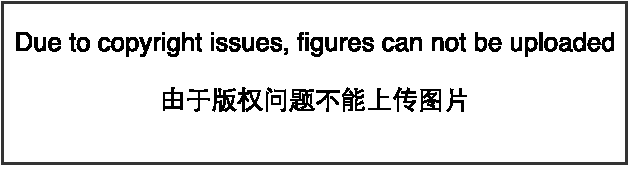
\includegraphics{figure.pdf}}
\else
\centerline{\includegraphics{Chapter6/figures/computational_graph}}
\fi
\captionsetup{singlelinecheck=off}
\caption{一些计算图的示例。
\emph{(a)}使用$\times$操作计算$z = xy$的图。 
\emph{(b)}用于\gls{logistic_regression}预测$\hat{y} = \sigma(\bm{x}^\top \bm{w} + b)$的图。 一些中间表达式在代数表达式中没有名称,但在图形中却需要。
我们简单地将第$i$个这样的变量命名为$u^{(i)}$。
\emph{(c)}表达式$\bm{H} = \max \{ 0, \bm{X}\bm{W}+ \bm{b} \}$的计算图,在给定包含小批量输入数据的设计矩阵$\bm{X}$时,它计算\gls{ReLU}激活的设计矩阵$\bm{H}$。
\emph{(d)}示例a-c对每个变量最多只实施一个操作,但是对变量实施多个操作也是可能的。 这里我们展示一个计算图,它对线性回归模型的权重$\bm{w}$实施多个操作。
这个权重不仅用于预测$\hat{y}$,也用于权重衰减罚项$\lambda \sum_i w_i^2$。}
\label{fig:chap6_computational_graph}
\end{figure}

\subsection{微积分中的链式法则}
\label{sec:chain_rule_of_calculus}

微积分中的链式法则(为了不与概率中的链式法则相混淆)用于计算复合函数的导数。
反向传播是一种计算链式法则的算法,使用高效的特定运算顺序。

设$x$是实数,$f$和$g$是从实数映射到实数的函数。
假设$y=g(x)$并且$z=f(g(x))=f(y)$。
那么链式法则是说
\begin{equation}
\frac{dz}{dx}=\frac{dz}{dy} \frac{dy}{dx}.
\label{eq:6.44}
\end{equation}

我们可以将这种标量情况进行扩展。
假设$\bm{x}\in \SetR^m, \bm{y}\in \SetR^n$,$g$是从$\SetR^m$到$\SetR^n$的映射,$f$是从$\SetR^n$到$\SetR$的映射。
如果$\bm{y}=g(\bm{x})$并且$z=f(\bm{y})$,那么
\begin{equation}
\frac{\partial z}{\partial x_i} = \sum_j \frac{\partial z}{\partial y_j} \frac{\partial y_j}{\partial x_i}.
\end{equation}
使用向量记法,可以等价地写成
\begin{equation}
\nabla_{\bm{x}}z = \left ( \frac{\partial \bm{y}}{\partial \bm{x}} \right )^\top \nabla_{\bm{y}} z,
\end{equation}
这里$\frac{\partial \bm{y}}{\partial \bm{x}}$是$g$的$n\times m$的\gls{jacobian_matrix}。

从这里我们看到变量$\bm{x}$的梯度可以通过\gls{jacobian_matrix}$\frac{\partial \bm{y}}{\partial \bm{x}}$和梯度$\nabla_{\bm{y}} z$相乘来得到。
反向传播算法由图中每一个这样的Jacobi梯度的乘积操作所组成。

% -- 199 --

通常我们不将反向传播算法仅用于向量,而是应用于任意维度的张量。
从概念上讲,这与使用向量的反向传播完全相同。 
唯一的区别是如何将数字排列成网格以形成张量。 
我们可以想象,在我们运行反向传播之前,将每个张量变平为一个向量,计算一个向量值梯度,然后将该梯度重新构造成一个张量。
从这种重新排列的观点上看,反向传播仍然只是将\gls{jacobian_matrix}乘以梯度。

% -- 200 --

为了表示值$z$对张量$\TSX$的梯度,我们记为$\nabla_\TSX z$,就像$\TSX$是向量一样。
$\TSX$的索引现在有多个坐标——例如,一个3维的张量由三个坐标索引。
我们可以通过使用单个变量$i$来表示完整的索引元组,从而完全抽象出来。
对所有可能的元组$i$,$(\nabla_\TSX z)_i$给出$\frac{\partial z}{\partial \TEX_i}$。
这与向量中索引的方式完全一致,$(\nabla_{\bm{x}} z)_i$给出$\frac{\partial z}{\partial x_i}$。
使用这种记法,我们可以写出适用于张量的链式法则。
如果$\TSY=g(\TSX)$并且$z=f(\TSY)$,那么
\begin{equation}
  \nabla_\TSX z = \sum_j (\nabla_\TSX \TEY_j)\frac{\partial z}{\partial \TEY_j}.
  \label{eq:6.47}
\end{equation}

\subsection{递归地使用链式法则来实现BP}
\label{sec:recursively_applying_the_chain_rule_to_obtain_backprop}

使用链式规则,可以直接写出某个标量对于计算图中任何产生该标量的节点的梯度的代数表达式。
然而,实际在计算机中计算该表达式时会引入一些额外的考虑。

具体来说,许多子表达式可能在梯度的整个表达式中重复若干次。
任何计算梯度的程序都需要选择是存储这些子表达式还是重新计算它们几次。
图\ref{fig:chap6_repeated_subexpression}给出了一个例子来说明这些重复的子表达式是如何出现的。
在某些情况下,计算两次相同的子表达式纯粹是浪费。
在复杂图中,可能存在指数多的这种计算上的浪费,使得简单的链式法则不可实现。
在其他情况下,计算两次相同的子表达式可能是以较高的运行时间为代价来减少内存开销的有效手段。

我们首先给出一个版本的反向传播算法,它指明了梯度的直接计算方式(算法\ref{alg:bprop}以及相关的正向计算的算法\ref{alg:fprop}),按照它实际完成的顺序并且递归地使用链式法则。
可以直接执行这些计算或者将算法的描述视为用于计算反向传播的计算图的符号表示。
然而,这些公式并没有明确地操作和构造用于计算梯度的符号图。
这些公式在后面的\ref{sec:general_back_propagation}节和算法\ref{alg:backprop}中给出,其中我们还推广到了包含任意张量的节点。

首先考虑描述如何计算单个标量$u^{(n)}$(例如训练样例上的损失函数)的计算图。
我们想要计算这个标量对$n_i$个输入节点$u^{(1)}$到$u^{(n_i)}$的梯度。
换句话说,我们希望对所有的$i\in\{1,2,\ldots,n_i\}$计算$\frac{\partial u^{(n)}}{\partial u^{(i)}}$。
在用反向传播计算梯度来实现参数的梯度下降时,$u^{(n)}$将对应单个或者小批量实例的代价函数,而$u^{(1)}$到$u^{(n_i)}$则对应于模型的参数。

% -- 201 --

我们将假设图的节点已经以一种特殊的方式被排序,使得我们可以一个接一个地计算他们的输出,从$u^{(n_i+1)}$开始,一直上升到$u^{(n)}$。
如算法\ref{alg:fprop}中所定义的,每个节点$u^{(i)}$与操作$f^{(i)}$相关联,并且通过对该函数求值来得到
\begin{equation}
  u^{(i)} = f(\SetA^{(i)}),
\end{equation}
其中$\SetA^{(i)}$是$u^{(i)}$所有父节点的集合。
% alg 6.1
\begin{algorithm}[htbp]
\caption{计算将$n_i$个输入$u^{(1)}$到$u^{(n_i)}$映射到一个输出$u^{(n)}$的程序。
这定义了一个计算图,其中每个节点通过将函数$f^{(i)}$应用到变量集合$\SetA^{(i)}$上来计算$u^{(i)}$的值,$\SetA^{(i)}$包含先前节点$u^{(j)}$的值满足$j<i$且$j \in Pa(u^{(i)})$。
计算图的输入是向量$\bm{x}$,并且被分配给前$n_i$个节点$u^{(1)}$到$u^{(n_i)}$。计算图的输出可以从最后一个节点$u^{(n)}$读出。}
\label{alg:fprop}
\begin{algorithmic}
\FOR {$i=1, \ldots, n_i$}
 \STATE $u^{(i)} \leftarrow x_i$
\ENDFOR
\FOR {$i=n_i+1, \ldots, n$}
 \STATE $\SetA^{(i)} \leftarrow \{ u^{(j)} \mid j \in Pa(u^{(i)}) \}$
 \STATE $u^{(i)} \leftarrow f^{(i)}(\SetA^{(i)})$
\ENDFOR
\STATE {\bf return} $u^{(n)}$
\end{algorithmic}
\end{algorithm}

% -- 202 --

该算法详细说明了前向传播的计算,我们可以将其放入图$\CalG$中。
为了执行反向传播,我们可以构造一个依赖于$\CalG$并添加额外一组节点的计算图。
这形成了一个子图$\CalB$,它的每个节点都是$\CalG$的节点。
$\CalB$中的计算和$\CalG$中的计算顺序完全相反,而且$\CalB$中的每个节点计算导数$\frac{\partial u^{(n)}}{\partial u^{(i)}}$与前向图中的节点$u^{(i)}$相关联。
这通过对标量输出$u^{(n)}$使用链式法则来完成
\begin{equation}
  \frac{\partial u^{(n)}}{\partial u^{(j)}} = \sum_{i:j \in Pa(u^{(i)})} \frac{\partial u^{(n)} }{ \partial u^{(i)} } \frac{ \partial u^{(i)} }{ \partial u^{(j)} }
  \label{eq:6.49}
\end{equation}
在算法\ref{alg:bprop}中详细说明。
子图$\CalB$恰好包含每一条对应着$\CalG$中从节点$u^{(j)}$到节点$u^{(i)}$的边。
从$u^{(j)}$到$u^{(i)}$的边对应着计算$\frac{\partial u^{(i)}}{\partial u^{(j)}}$。
另外,对于每个节点都要执行一个内积,内积的一个因子是对于$u^{j}$孩子节点$u^{(i)}$的已经计算的梯度,另一个因子是对于相同孩子节点$u^{(i)}$ 的偏导数$\frac{\partial u^{(i)}}{\partial u^{(j)}}$组成的向量。
总而言之,执行反向传播所需的计算量与$\CalG$中的边的数量成比例,其中每条边的计算包括计算偏导数(节点关于它的一个父节点的偏导数)以及执行一次乘法和一次加法。
下面,我们将此分析推广到张量值节点,这只是在同一节点中对多个标量值进行分组并能够更有效的实现。
% fig 6.9
\begin{figure}[!htb]
\ifOpenSource
\centerline{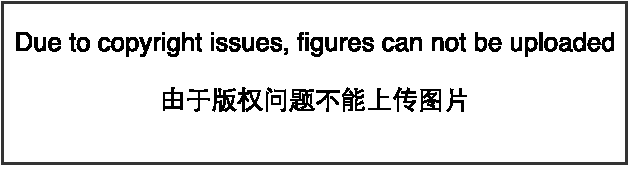
\includegraphics{figure.pdf}}
\else
\centerline{\includegraphics{Chapter6/figures/repeated_subexpression}}
\fi
\captionsetup{singlelinecheck=off}
\caption[.]{
计算梯度时导致重复子表达式的计算图。
令$w \in \SetR$为图的输入。
我们对链中的每一步使用相同的操作函数$f: \SetR \to \SetR$,这样$x=f(w), y=f(x), z=f(y)$。
为了计算$\frac{\partial z}{\partial w}$,我们应用公式\ref{eq:6.44}得到:
\begin{align}
& \frac{\partial z}{\partial w}\\
=& \frac{\partial z}{\partial y} \frac{\partial y}{\partial x} \frac{\partial x}{\partial w}\\
\label{eq:6.52}
=& f'(y)f'(x)f'(w)\\ 
\label{eq:6.53}
=& f'(f(f(w))) f'(f(w)) f'(w). 
\end{align}
公式\ref{eq:6.52}建议我们采用的实现方式是,仅计算$f(w)$的值一次并将它存储在变量$x$中。
这是\gls{BP}算法所采用的方法。
公式\ref{eq:6.53}提出了一种替代方法,其中子表达式$f(w)$出现了不止一次。 %这里不知道怎么弄多个label的公式,会报错
在替代方法中,每次只在需要时重新计算$f(w)$。
当存储这些表达式的值所需的存储较少时,公式\ref{eq:6.52}的\gls{BP}方法显然是较优的,因为它减少了运行时间。
然而,公式\ref{eq:6.53}也是链式法则的有效实现,并且当存储受限时它是有用的。}
\label{fig:chap6_repeated_subexpression}
\end{figure}

% -- 203 --

反向传播算法被设计为减少公共子表达式的数量而不考虑存储的开销。
具体来说,它大约对图中的每个节点执行一个Jacobi乘积。
这可以从算法\ref{alg:bprop}中看出,反向传播算法访问了图中的节点$u^{(j)}$到节点$u^{(i)}$的每条边一次,以获得相关的偏导数$\frac{\partial u^{(i)}}{\partial u^{(j)}}$。
反向传播因此避免了重复子表达式的指数爆炸。
然而,其他算法可能通过对计算图进行简化来避免更多的子表达式,或者也可能通过重新计算而不是存储这些子表达式来节省内存。
我们将在描述完反向传播算法本身后再重新审视这些想法。
% alg 6.2
\begin{algorithm}[htb!]
\caption{\gls{BP}算法的简化版本,用于计算$u^{(n)}$对图中变量的导数。
这个示例旨在通过演示所有变量都是标量的简化情况来进一步理解\gls{BP}算法,这里我们希望计算关于$u^{(1)},\ldots,u^{(n_i)}$的导数。
这个简化版本计算了关于图中所有节点的导数。
假定与每条边相关联的偏导数计算需要恒定的时间的话,该算法的计算成本与图中边的数量成比例。
这与\gls{forward_propagation}的计算次数具有相同的阶。
每个$\frac{\partial u^{(i)}}{\partial u^{(j)}}$是$u^{(i)}$的父节点$u^{(j)}$的函数,从而将前向图的节点链接到\gls{BP}图中添加的节点。}
\label{alg:bprop}
\begin{algorithmic}
\STATE Run forward propagation (algorithm \ref{alg:fprop} for this example) to obtain
the activations of the network
\STATE Initialize {\tt grad\_table}, a data structure that will store the derivatives
that have been computed. The entry ${\tt grad\_table}[u^{(i)}]$ will store the computed
value of $\frac{\partial u^{(n)}}{\partial u^{(i)}}$.
\STATE ${\tt grad\_table}[u^{(n)}] \leftarrow 1$
\FOR {$j=n-1$ down to 1}
\STATE The next line computes $\frac{\partial u^{(n)}}{\partial u^{(j)}} =
  \sum_{i: j \in Pa(u^{(i)})} \frac{\partial u^{(n)}}{\partial u^{(i)}} \frac{\partial u^{(i)}}{\partial u^{(j)}}$ using stored values:
\STATE ${\tt grad\_table}[ u^{(j)}] \leftarrow 
\sum_{i: j \in Pa(u^{(i)})} {\tt grad\_table}[u^{(i)}]
\frac{\partial u^{(i)}}{\partial u^{(j)}}$
\ENDFOR
\STATE {\bf return} $\{ {\tt grad\_table}[ u^{(i)}] \mid i=1, \dots, n_i \} $
\end{algorithmic}
\end{algorithm}


% -- 204 --

\subsection{全连接MLP中BP的计算}
\label{sec:back_propagation_computation_in_fully_connected_mlp}

为了阐明反向传播的上述定义,让我们考虑一个与全连接的多层MLP相关联的特定图。

算法\ref{alg:mlp-fprop}首先给出了前向传播,它将参数映射到与单个训练样例(输入,目标)$(\bm{x},\bm{y})$相关联的有监督损失函数$L(\hat{\bm{y}}, \bm{y})$,其中$\hat{\bm{y}}$是当$\bm{x}$提供输入时神经网络的输出。
% alg 6.3
\begin{algorithm}[ht]
\caption{典型深度神经网络中的\gls{forward_propagation}和代价函数的计算。
损失函数$L(\hat{\Vy},\Vy)$取决于输出$\hat{\Vy}$和目标$\Vy$(参见\ref{sec:learning_conditional_distributions_with_maximum_likelihood}节中损失函数的示例)。
为了获得总代价$J$,损失函数可以加上正则项$\Omega(\theta)$,其中$\theta$包含所有参数(权重和偏置)。
算法\ref{alg:mlp-bprop}说明了如何计算$J$对参数$\bm{W}$和$\bm{b}$的梯度。 为简单起见,该演示仅使用单个输入样例$\Vx$。
实际应用应该使用\gls{minibatch}。
请参见\ref{sec:example_back_propagation_for_mlp_training}以获得更加真实的演示。}
\label{alg:mlp-fprop}
\begin{algorithmic}
\REQUIRE Network depth, $l$
\REQUIRE $\MW^{(i)}, i \in \{ 1, \dots, l\},$ the weight matrices of the model
\REQUIRE $\Vb^{(i)}, i \in \{ 1, \dots, l\},$ the bias parameters of the model
\REQUIRE $\Vx$, the input to process
\REQUIRE $\Vy$, the target output
\STATE $\Vh^{(0)}=\Vx$
\FOR {$k=1, \ldots, l$}
 \STATE $\Va^{(k)} = \Vb^{(k)} + \MW^{(k)} \Vh^{(k-1)}$
 \STATE $\Vh^{(k)} = f(\Va^{(k)})$
\ENDFOR
\STATE $\hat{\Vy} = \Vh^{(l)}$
\STATE $J = L(\hat{\Vy},\Vy) + \lambda \Omega(\theta)$
\end{algorithmic}
\end{algorithm}

算法\ref{alg:mlp-bprop}随后说明了将反向传播应用于改图所需的相关计算。
% alg 6.4
\begin{algorithm}[htbp]
\caption{深度神经网络中算法\ref{alg:mlp-fprop}的反向计算,它使用了不止输入$\Vx $和目标$\bm{y}$。
该计算对于每一层$k$都产生了对激活$\Va^{(k)}$的梯度,从输出层开始向后计算一直到第一个\gls{hidden_layer}。
这些梯度可以看作是对每层的输出应如何调整以减小误差的指导,根据这些梯度可以获得对每层参数的梯度。
权重和偏置上的梯度可以立即用作随机梯度更新的一部分(梯度算出后即可执行更新),或者与其他基于梯度的优化方法一起使用。
}
\label{alg:mlp-bprop}
\begin{algorithmic}
\STATE After the forward computation, compute the gradient on the output layer:
\STATE $\Vg \leftarrow \nabla_{\hat{\Vy}} J = \nabla_{\hat{\Vy}} L(\hat{\Vy},\Vy)$
\FOR {$k=l, l-1, \dots, 1$}
\STATE Convert the gradient on the layer's output into a gradient into the pre-nonlinearity activation
       (element-wise multiplication if $f$ is element-wise):
  \STATE $\Vg \leftarrow \nabla_{\Va^{(k)}} J = \Vg \odot f'(\Va^{(k)})$
  \STATE Compute gradients on weights and biases (including the regularization term, where needed):
  \STATE $\nabla_{\Vb^{(k)}} J = \Vg + \lambda \nabla_{\Vb^{(k)}} \Omega(\theta)$
  \STATE $\nabla_{\MW^{(k)}} J = \Vg \; \Vh^{(k-1)\top} + \lambda \nabla_{\MW^{(k)}} \Omega(\theta)$
  \STATE Propagate the gradients w.r.t. the next lower-level hidden layer's activations:
  \STATE $\Vg \leftarrow \nabla_{\Vh^{(k-1)}} J = \MW^{(k)\top} \; \Vg$
\ENDFOR
\end{algorithmic}
\end{algorithm}

算法\ref{alg:mlp-fprop}和算法\ref{alg:mlp-bprop}是简单而直观的演示。
然而,它们专门针对特定的问题。

现在的软件实现基于之后\ref{sec:general_back_propagation}节中描述的一般形式的反向传播,它可以通过明确地操作用于表示符号计算的数据结构,来适应任何计算图。


% -- 205 --

\subsection{符号到符号的导数}
\label{sec:symbol_to_symbol_derivatives}

代数表达式和计算图都对\firstgls{symbol}或不具有特定值的变量进行操作。
这些代数或者基于图的表达式被称为\firstgls{symbolic_representation}。
当我们实际使用或者训练神经网络时,我们必须给这些符号赋值。
我们用一个特定的\firstgls{numeric_value}来替代网络的符号输入$\bm{x}$,例如$[1.2, 3,765, -1.8]^\top$。

一些反向传播的方法采用计算图和一组用于图的输入的数值,然后返回在这些输入值处梯度的一组数值。
我们将这种方法称为``符号到数值''的微分。
这种方法用在诸如Torch\citep{Torch-2011}和Caffe\citep{Jia13caffe}之类的库中。

% -- 206 --
 
另一种方法是采用计算图以及添加一些额外的节点到计算图中,这些额外的节点提供了我们所需导数的符号描述。
这是Theano\citep{bergstra+al:2010-scipy-small,Bastien-Theano-2012}和TensorFlow\citep{tensorflow}采用的方法。
图\ref{fig:chap6_symbol_to_symbol}给出了该方法如何工作的一个例子。
这种方法的主要优点是导数可以使用与原始表达式相同的语言来描述。
因为导数只是另外一张计算图,可以再次运行反向传播,对导数再进行求导以得到更高阶的导数。
高阶导数的计算在\ref{sec:higher_order_derivatives}中描述。
% fig 6.10
\begin{figure}[!htb]
\ifOpenSource
\centerline{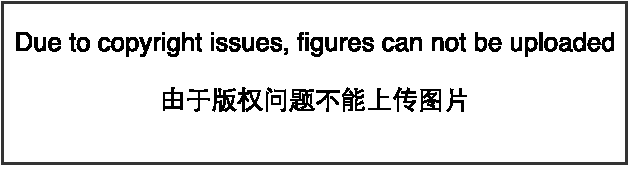
\includegraphics{figure.pdf}}
\else
\centerline{\includegraphics{Chapter6/figures/symbol_to_symbol}}
\fi
\captionsetup{singlelinecheck=off}
\caption{使用符号到符号的方法计算导数的示例。
在这种方法中,\gls{BP}算法不需要访问任何实际的特定数值。
相反,它将节点添加到计算图中来描述如何计算这些导数。
通用图形求值引擎可以在随后计算任何特定数值的导数。
\emph{(左)}在这个例子中,我们从表示$z=f(f(f(w)))$的图开始。
\emph{(右)}我们运行\gls{BP}算法,指导它构造表达式$\frac{dz}{dw}$对应的图。 在这个例子中,我们不解释\gls{BP}算法如何工作。
我们的目的只是说明想要的结果是什么:具有导数的符号描述的计算图。}
\label{fig:chap6_symbol_to_symbol}
\end{figure}

我们将使用后一种方法,并且使用构造导数的计算图的方法来描述反向传播算法。
图的任意子集后来都可以使用特定的数值来求值。
这允许我们避免完全指明每个操作应该在何时计算。
相反,通用的图计算引擎只要当一个节点的父节点的值都可用时就可以进行求值。

% -- 207 --
  
基于符号到符号的方法的描述包含了符号到数值的方法。
符号到数值的方法可以理解为执行了与符号到符号的方法中构建图的过程中完全相同的计算。
关键的区别是符号到数值的方法不会显示出图形。

\subsection{一般化的BP}
\label{sec:general_back_propagation}

反向传播算法非常简单。
为了计算某个标量$z$对图中它的一个祖先$\bm{x}$的梯度,我们首先观察到对$z$的梯度由$\frac{dz}{dz}=1$给出。
我们然后可以计算对图中$z$的每个父节点的梯度,通过现有的梯度乘以产生$z$的操作的\gls{jacobian_matrix}。
我们继续乘以\gls{jacobian_matrix},以这种方式向后穿过图,直到我们到达$\bm{x}$。
对于从$z$出发可以经过两个或更多路径向后行进而到达的任意节点,我们简单的对该节点来自不同路径上的梯度进行求和。

更正式地,图$\CalG$中的每个节点对应着一个变量。
为了实现最大的一般化,我们将这个变量描述为一个张量$\TSV$。
张量通常可以具有任意维度,并且包含标量、向量和矩阵。

我们假设每个变量$\TSV$与下列子程序相关联:
\begin{itemize}
    \item \verb|get_operation|($\TSV$):它返回用于计算$\TSV$的操作,代表了在计算图中流入$\TSV$的边。
    例如,可能有一个Python或者C++的类表示矩阵乘法操作,以及\verb|get_operation|函数。
    假设我们的一个变量是由矩阵乘法产生的,$\bm{C}=\bm{A}\bm{B}$。
    那么,\verb|get_operation|($\TSV$)返回一个指向相应C++类的实例的指针。

    \item \verb|get_consumers|($\TSV, \CalG$):它返回一组变量,是计算图$\CalG$中$\TSV$的孩子节点。

    \item \verb|get_inputs|($\TSV, \CalG$):它返回一组变量,是计算图$\CalG$中$\TSV$的父节点。
\end{itemize}

% -- 208 --
  
每个操作\verb|op|也与\verb|bprop|操作相关联。
该\verb|bprop|操作可以计算如公式\ref{eq:6.47}所描述的Jacobi向量积。
这是反向传播算法能够实现很大通用性的原因。
每个操作负责了解如何通过它参与的图中的边来反向传播。
例如,我们可以使用矩阵乘法操作来产生变量$\bm{C}=\bm{A}\bm{B}$。
假设标量$z$关于$\bm{C}$的梯度是$\bm{G}$。
矩阵乘法操作负责定义两个反向传播规则,每个规则对应于一个输入变量。
如果我们调用\verb|bprop|方法来请求$\bm{A}$的梯度,在给定输出的梯度为$\bm{G}$ 的情况下,那么矩阵乘法操作的\verb|bprop|方法必须说明对$\bm{A}$的梯度是$\bm{G}\bm{B}^\top$。
类似的,如果我们调用\verb|bprop|方法来请求$\bm{B}$的梯度,那么矩阵操作负责实现\verb|bprop|方法并指定期望的梯度是$\bm{A}^\top\bm{G}$。
反向传播算法本身并不需要知道任何微分法则。
它只需要使用正确的参数调用每个操作的\verb|bprop|方法即可。
正式地,\verb|op.bprop(inputs|$, \TSX, \TSG)$必须返回
\begin{equation}
  \sum_i (\nabla_{\TSX} \verb|op.f(inputs|)_i) \textsf{G}_i,
\end{equation}
这只是如公式\ref{eq:6.47}所表达的链式法则的实现。
这里,\verb|inputs|是提供给操作的一组输入,\verb|op.f|是操作实现的数学函数,$\TSX$是输入,我们想要计算关于它的梯度,$\TSG$是操作对于输出的梯度。

\verb|op.bprop|方法应该总是假装它的所有输入彼此不同,即使它们不是。
例如,如果\verb|mul|操作传递两个$x$来计算$x^2$,\verb|op.bprop|方法应该仍然返回$x$作为对于两个输入的导数。
反向传播算法后面会将这些变量加起来获得$2x$,这是$x$上总的正确的导数。

反向传播算法的软件实现通常提供操作和其\verb|bprop|两种方法,所以深度学习软件库的用户能够对使用诸如矩阵乘法、指数运算、对数运算等等常用操作构建的图进行反向传播。
构建反向传播新实现的软件工程师或者需要向现有库添加自己的操作的高级用户通常必须手动为新操作推导\verb|op.bprop|方法。

反向传播算法的正式描述参见算法\ref{alg:backprop}。

% -- 209 --
% alg 6.5
\begin{algorithm}[ht]
\caption{\gls{BP}算法最外围的骨架。
这部分做简单的设置和清理工作。
大多数重要的工作在发生在算法\ref{alg:build_grad}的子程序{\tt build\_grad}中。
}
\label{alg:backprop}
\begin{algorithmic}
\REQUIRE $\SetT$, the target set of variables whose gradients must be computed.
\REQUIRE $\CalG$, the computational graph
\REQUIRE $z$, the variable to be differentiated
\STATE Let $\CalG'$ be $\CalG$ pruned to contain only nodes that are ancestors
of $z$ and descendents of nodes in $\SetT$.
\STATE Initialize {\tt grad\_table}, a data structure associating tensors
to their gradients
\STATE ${\tt grad\_table}[z] \leftarrow 1$
\FOR{$\TSV$ in $\SetT$}
\STATE ${\tt build\_grad}(\TSV, \CalG, \CalG', {\tt grad\_table})$
\ENDFOR
\STATE Return {\tt grad\_table} restricted to $\SetT$
\end{algorithmic}
\end{algorithm}

\begin{algorithm}[ht]
\caption{\gls{BP}算法的内循环子程序${\tt build\_grad}(\TSV, \CalG, \CalG', {\tt grad\_table})$,
被在算法\ref{alg:backprop}中定义的\gls{BP}算法调用。
}
\label{alg:build_grad}
\begin{algorithmic}
\REQUIRE $\TSV$, the variable whose gradient should be added to $\CalG$
and {\tt grad\_table}.
\REQUIRE $\CalG$, the graph to modify.
\REQUIRE $\CalG'$, the restriction of $\CalG$ to nodes that participate
in the gradient.
\REQUIRE {\tt grad\_table}, a data structure mapping nodes to their
gradients
\IF{$\SetV$ is in {\tt grad\_table} }
 \STATE Return ${\tt grad\_table}[\TSV]$
\ENDIF
\STATE $i \leftarrow 1$
\FOR{$\TSC$ in ${\tt get\_consumers}(\TSV, \CalG')$ }
\STATE ${\tt op} \leftarrow {\tt get\_operation}(\TSC)$
\STATE $\TSD \leftarrow {\tt build\_grad}(\TSC, \CalG, \CalG', {\tt grad\_table})$
\STATE $\TSG^{(i)} \leftarrow {\tt op.bprop}({\tt get\_inputs}(\TSC, \CalG'), \TSV, \TSD)$ 
\STATE $i \leftarrow i + 1$
\ENDFOR
\STATE $\TSG \leftarrow \sum_i \TSG^{(i)}$
\STATE ${\tt grad\_table}[\TSV] = \TSG$
\STATE Insert $\TSG$ and the operations creating it into $\CalG$
\STATE Return $\TSG$
\end{algorithmic}
\end{algorithm}


% -- 210 --
  
在\ref{sec:chain_rule_of_calculus}节中,我们使用反向传播作为一种策略来避免多次计算链式法则中的相同子表达式。
由于这些重复子表达式的存在,简单的算法可能具有指数运行时间。
现在我们已经详细说明了反向传播算法,我们可以去理解它的计算成本。
如果我们假设每个操作的执行都有大致相同的开销,那么我们可以依据执行操作的数量来分析计算成本。
注意这里我们将一个操作记为计算图的基本单位,它实际可能包含许多算术运算(例如,我们可能将矩阵乘法视为单个操作)。
在具有$n$个节点的图中计算梯度,将永远不会执行超过$O(n^2)$个操作,或者存储超过$O(n^2)$个操作的输出。
这里我们是对计算图中的操作进行计数,而不是由底层硬件执行的单独操作,所以重要的是要记住每个操作的运行时间可能是高度可变的。
例如,两个矩阵相乘可能对应着图中的一个单独的操作,但这两个矩阵可能每个都包含数百万个元素。
我们可以看到,计算梯度至多需要$O(n^2)$的操作,因为在最坏的情况下,前向传播的步骤将执行原始图的全部$n$个节点(取决于我们想要计算的值,我们可能不需要执行整个图)。
反向传播算法在原始图的每条边添加一个Jacobi向量积,可以用$O(1)$个节点来表达。
因为计算图是有向无环图,它至多有$O(n^2)$条边。对于实践中常用的图的类型,情况会更好。
大多数神经网络的代价函数大致是链式结构的,使得反向传播只有$O(n)$的成本。
这远远胜过简单的方法,简单方法可能需要执行指数级的节点。
这种潜在的指数级代价可以通过非递归地扩展和重写递归链式法则(公式
\ref{eq:6.49})来看出:
\begin{equation}
  \frac{\partial u^{(n)}}{\partial u^{(j)}} =
  \sum_{\substack{\text{path}(u^{(\pi_1)}, u^{(\pi_2)}, \ldots, u^{(\pi_t)}  ),\\ \text{from } \pi_1=j \text{ to }\pi_t = n}}
  \prod_{k=2}^t \frac{\partial u^{(\pi_k)}}{\partial u^{(\pi_{k-1})}}.
\end{equation}
由于节点$j$到节点$n$的路径数目可以在这些路径的长度上指数地增长,所以上述求和符号中的项数(这些路径的数目),可能以前向传播图的深度的指数级增长。
会产生如此大的成本是因为对于$\frac{\partial u^{(i)}}{\partial u^{(j)}}$,相同的计算会重复进行很多次。
为了避免这种重新计算,我们可以将反向传播看作一种表填充算法,利用存储的中间结果$\frac{\partial u^{(n)}}{\partial u^{(i)}}$来对表进行填充。
图中的每个节点对应着表中的一个位置,这个位置存储对该节点的梯度。
通过顺序填充这些表的条目,反向传播算法避免了重复计算许多公共子表达式。
这种表填充策略有时被称为\firstgls{dynamic_programming}。
  
% -- 211 --
  
\subsection{实例:用于MLP训练的BP}
\label{sec:example_back_propagation_for_mlp_training}

作为一个例子,我们利用反向传播算法来训练多层感知器。

这里,我们考虑具有单个\gls{hidden_layer}的一个非常简单的多层感知机。
为了训练这个模型,我们将使用小批量(minibatch)随机梯度下降算法。
反向传播算法用于计算单个minibatch上的代价的梯度。
具体来说,我们使用训练集上的一组minibatch实例,将其规范化为一个设计矩阵$\bm{X}$以及相关联的类标签的向量$\bm{y}$。
网络计算隐藏特征层$\bm{H}=\max\{0, \bm{X}\bm{W}^{(1)}\}$。
为了简化表示,我们在这个模型中不使用偏置。
假设我们的图语言包含\verb|relu|操作,该操作可以对$\max\{0,\bm{Z}\}$表达式的每个元素分别进行计算。
类的非归一化对数概率的预测将随后由$\bm{H}\bm{W}^{(2)}$ 给出。
假设我们的图语言包含\verb|cross_entropy|操作,用以计算目标$\bm{y}$和由这些未归一化对数概率定义的概率分布间的\gls{cross_entropy}。
所得到的\gls{cross_entropy}定义了代价函数$J_\text{MLE}$。最小化这个\gls{cross_entropy}将执行对分类器的最大似然估计。
然而,为了使得这个例子更加真实,我们也包含一个正则项。
总的代价函数为
\begin{equation}
  J = J_{\text{MLE}} + \lambda \left ( \sum_{i, j} \left (W_{i, j}^{(1)} \right )^2 + \sum_{i, j} \left (W_{i, j}^{(2)} \right)^2 \right )
\end{equation}
包含了\gls{cross_entropy}和系数为$\lambda$的权重衰减项。
它的计算图在图\ref{fig:chap6_mlp_example}中给出。
% fig 6.11
\begin{figure}[!htb]
\ifOpenSource
\centerline{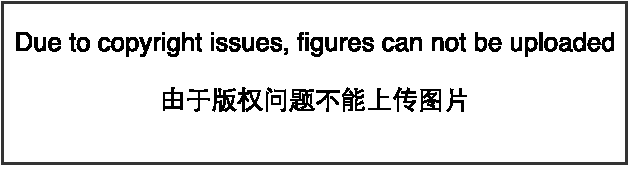
\includegraphics{figure.pdf}}
\else
\centerline{\includegraphics{Chapter6/figures/mlp_example}}
\fi
\caption{用于计算代价函数的计算图,这个代价函数是使用\gls{cross_entropy}损失以及权重衰减训练我们的单层\glssymbol{MLP}示例所产生的。}
\label{fig:chap6_mlp_example}
\end{figure}

这个示例的梯度计算图实在太大,以至于绘制或者阅读都将是乏味的。
这显示出了反向传播算法的优点之一,即它可以自动生成梯度,而这种计算对于软件工程师来说需要进行直观但冗长的手动推导。

我们可以通过观察图\ref{fig:chap6_mlp_example}中的正向传播图来粗略地描述反向传播算法的行为。
为了训练,我们希望计算$\nabla_{\bm{W}^{(1)}} J$和$\nabla_{\bm{W}^{(2)}} J$。
有两种不同的路径从$J$后退到权重:一条通过\gls{cross_entropy}成本,另一条通过权重衰减成本。
权重衰减成本相对简单,它总是对$\bm{W}^{(i)}$上的梯度贡献$2\lambda \bm{W}^{(i)}$。
  
% -- 212 --
  
另一条通过\gls{cross_entropy}成本的路径稍微复杂一些。
令$\bm{G}$是由\verb|cross_entropy|操作提供的对未归一化对数概率$\bm{U}^{(2)}$的梯度。
反向传播算法现在需要探索两个不同的分支。
在较短的分支上,它使用对矩阵乘法的第二个变量的反向传播规则,将$\bm{H}^\top \bm{G}$加到$\bm{W}^{(2)}$的梯度上。
另一条更长些的路径沿着网络逐步下降。
首先,反向传播算法使用对矩阵乘法的第一个变量的反向传播规则,计算$\nabla_{\bm{H}} J = \bm{G}\bm{W}^{(2)\top}$。
接下来,\verb|relu|操作使用其反向传播规则来对关于$\bm{U}^{(1)}$的梯度中小于0的部分清零。记上述结果为$\bm{G}'$。 
反向传播算法的最后一步是使用对\verb|matmul|操作的第二个变量的反向传播规则,将$\bm{X}^\top \bm{G}'$加到$\bm{W}^{(1)}$的梯度上。

在计算了这些梯度以后,梯度下降算法或者其他的优化算法的责任就是使用这些梯度来更新参数。

对于MLP,计算成本主要来源于矩阵乘法。
在前向传播阶段,我们乘以每个权重矩阵,得到了$O(w)$数量的乘-加,其中$w$是权重的数量。
在反向传播阶段,我们乘以每个权重矩阵的转置,具有相同的计算成本。
算法主要的存储成本是我们需要将输入存储到\gls{hidden_layer}的非线性中去。
这些值从被计算时开始存储,直到反向过程回到了同一点。
因此存储成本是$O(mn_h)$,其中$m$是minibatch中样例的数目,$n_h$是\gls{hidden_unit}的数量。
  
% -- 213 --
  
\subsection{复杂化}
\label{sec:complications}

我们这里描述的反向传播算法要比现实中实际使用的实现要简单。

正如前面提到的,我们将操作的定义限制为返回单个张量的函数。
大多数软件实现需要支持可以返回多个张量的操作。 
例如,如果我们希望计算张量中的最大值和该值的索引,则最好在单次运算中计算两者,因此将该过程实现为具有两个输出的操作效率更高。

我们还没有描述如何控制反向传播的内存消耗。
反向传播经常涉及将许多张量加在一起。
在朴素方法中,将分别计算这些张量中的每一个,然后在第二步中对所有这些张量求和。 
朴素方法具有过高的存储瓶颈,可以通过保持一个缓冲器,并且在计算时将每个值加到该缓冲器中来避免该瓶颈。

反向传播的现实实现还需要处理各种数据类型,例如32位浮点数,64位浮点数和整型。
处理这些类型的策略需要特别的设计考虑。

一些操作具有未定义的梯度,并且重要的是跟踪这些情况并且确定用户请求的梯度是否是未定义的。

各种其他技术的特性使现实世界的微分更加复杂。 这些技术性并不是不可逾越的,本章已经描述了计算微分所需的关键智力工具,但重要的是要知道还有许多的精妙之处存在。
  
% -- 214 --
  
\subsection{深度学习界以外的微分}
\label{sec:differentiation_outside_the_deep_learning_community}

深度学习界在某种程度上已经与更广泛的计算机科学界隔离开来,并且在很大程度上发展了自己关于如何进行微分的文化态度。
更一般地,\firstgls{automatic_differentiation}领域关心如何以算法方式计算导数。 
这里描述的反向传播算法只是自动微分的一种方法。 
它是一种称为\firstgls{reverse_mode_accumulation}的更广泛类型的技术的特殊情况。 
其他方法以不同的顺序来计算链式法则的子表达式。 
一般来说,确定一种计算的顺序使得计算开销最小,是困难的问题。 
找到计算梯度的最优操作序列是NP完全问题\citep{naumann2008optimal},在这种意义上,它可能需要将代数表达式简化为它们最廉价的形式。

例如,假设我们有变量$p_1,p_2\ldots,p_n$表示概率,和变量$z_1,z_2,\ldots,z_n$表示未归一化的对数概率。
假设我们定义
\begin{equation}
  q_i = \frac{\exp(z_i)}{\sum_i \exp(z_i)},
\end{equation}
其中我们通过指数化、求和与除法运算构建softmax函数,并构造\gls{cross_entropy}损失函数$J=-\sum_i p_i\log q_i$。
人类数学家可以观察到$J$对$z_i$的导数采用了非常简单的形式:$p_iq_i-p_i$。
\footnote{译者注:这里作者误写成了$q_i-p_i$。}
反向传播算法不能够以这种方式来简化梯度,而是会通过原始图中的所有对数和指数操作显示地传播梯度。
一些软件库如Theano\citep{bergstra+al:2010-scipy-small,Bastien-Theano-2012}能够执行某些种类的代数替换来改进由纯反向传播算法提出的图。
  
% -- 215 --
  
当前向图$\CalG$具有单个输出节点,并且每个偏导数$\frac{\partial u^{(i)}}{\partial u^{(j)}}$都可以用恒定的计算量来计算时,反向传播保证梯度计算的计算数目和前向计算的计算数目是同一个量级:这可以在算法\ref{alg:bprop}中看出,因为每个局部偏导数$\frac{\partial u^{(i)}}{\partial u^{(j)}}$以及递归链式公式(公式\ref{eq:6.49})中相关的乘和加都只需计算一次。
因此,总的计算量是$O(\#\text{edges})$。
然而,可能通过对反向传播算法构建的计算图进行简化来减少这些计算量,并且这是NP完全问题。
诸如Theano和TensorFlow的实现使用基于匹配已知简化模式的试探法,以便重复地尝试去简化图。
我们定义反向传播仅用于计算标量输出的梯度,但是反向传播可以扩展到计算\gls{jacobian_matrix}(该\gls{jacobian_matrix}或者来源于图中的$k$个不同标量节点,或者来源于包含$k$个值的张量值节点)。
朴素的实现可能需要$k$倍的计算:对于原始前向图中的每个内部标量节点,朴素的实现计算$k$个梯度而不是单个梯度。
当图的输出数目大于输入的数目时,有时更偏向于使用另外一种形式的自动微分,称为\firstgls{forward_mode_accumulation}。
前向模式计算已经被提出用于循环神经网络梯度的实时计算,例如\citep{Williams89b}。
这也避免了存储整个图的值和梯度的需要,是计算效率和内存使用的折中。
前向模式和后向模式的关系类似于左乘和右乘一系列矩阵之间的关系,例如
\begin{equation}
  \bm{ABCD},
\end{equation}
其中的矩阵可以认为是\gls{jacobian_matrix}。
例如,如果$\bm{D}$是列向量,而$\bm{A}$有很多行,那么这对应于一幅具有单个输出和多个输入的图,并且从最后开始乘,反向进行,只需要矩阵-向量的乘积。
这对应着反向模式。
相反,从左边开始乘将涉及一系列的矩阵-矩阵乘积,这使得总的计算变得更加昂贵。
然而,如果$\bm{A}$的行数小于$D$的列数,则从左到右乘更为便宜,这对应着前向模式。

在机器学习以外的许多社区中,更常见的是使用传统的编程语言来直接实现微分软件,例如用Python或者C来编程,并且自动生成使用这些语言编写的不同函数的程序。
在深度学习界中,计算图通常使用由专用库创建的明确的数据结构表示。
专用方法的缺点是需要库开发人员为每个操作定义\verb|bprop|方法,并且限制了库的用户仅使用定义好的那些操作。
然而,专用方法也允许定制每个操作的反向传播规则,允许开发者以非显而易见的方式提高速度或稳定性,对于这种方式自动的过程可能不能复制。

因此,反向传播不是计算梯度的唯一方式或最佳方式,但它是一个非常实用的方法,继续为深度学习社区服务。 
在未来,深度网络的微分技术可能会提高,因为深度学习的从业者更加懂得了更广泛的自动微分领域的进步。
  
% -- 216 --
  
\subsection{高阶微分}
\label{sec:higher_order_derivatives}

一些软件框架支持使用高阶导数。 
在深度学习软件框架中,这至少包括Theano和TensorFlow。
这些库使用一种数据结构来描述要被微分的原始函数,它们使用相同类型的数据结构来描述这个函数的导数表达式。
这意味着符号微分机制可以应用于导数(从而产生高阶导数)。

在深度学习的相关领域,很少会计算标量函数的单个二阶导数。
相反,我们通常对Hessian矩阵的性质比较感兴趣。
如果我们有函数$f:\SetR^n \to \SetR$,那么Hessian矩阵的大小是$n\times n$。
在典型的深度学习应用中,$n$将是模型的参数数量,可能很容易达到数十亿。
完整的Hessian矩阵因此甚至不能表示。

代替明确地计算Hessian矩阵,典型的深度学习方法是使用\firstgls{Krylov_methods}。
Krylov方法是用于执行各种操作的一组迭代技术,这些操作包括像近似求解矩阵的逆、或者近似矩阵的特征值或特征向量等,而不使用矩阵-向量乘法以外的任何操作。

为了在Hesssian矩阵上使用Krylov方法,我们只需要能够计算Hessian矩阵$\bm{H}$和一个任意向量$\bm{v}$间的乘积即可。
实现这一目标的一种直观方法\citep{christianson1992automatic}是
\begin{equation}
  \bm{Hv}=\nabla_{\bm{x}} \left [ (\nabla_{\bm{x}} f(x))^\top \bm{v}\right ].
\end{equation}
该表达式中两个梯度的计算都可以由适当的软件库自动完成。
注意,外部梯度表达式是内部梯度表达式的函数的梯度。

如果$\bm{v}$本身是由计算图产生的一个向量,那么重要的是指定自动微分软件不要对产生$\bm{v}$的图进行微分。

虽然计算Hessian通常是不可取的,但是可以使用Hessian向量积。
可以对所有的$i=1,\ldots,n$简单地计算$\bm{He}^{(i)}$,其中$\bm{e}^{(i)}$是$e_i^{(i)}=1$并且其他元素都为0的\gls{one_hot}向量。

\section{历史小记}
\label{sec:historical_notes}

\gls{feedforward_network}可以被视为一种高效的非线性函数逼近器,它以使用梯度下降来最小化函数近似误差为基础。
从这个角度来看,现代\gls{feedforward_network}是一般函数近似任务的几个世纪进步的结晶。
  
% -- 217 --
  
处于反向传播算法底层的链式法则是17世纪发明的\citep{Leibniz-1676,LHopital-1696}。
微积分和代数长期以来被用于求解优化问题的封闭形式,但梯度下降直到19世纪才作为优化问题的一种迭代近似的求解方法被引入\citep{cauchy1847}。

从20世纪40年代开始,这些函数近似技术被用于导出诸如感知机的机器学习模型。 
然而,最早的模型都是基于线性模型。 
来自包括Marvin Minsky的批评指出了线性模型族的几个缺陷,例如它无法学习XOR函数,这导致了对整个神经网络方法的抵制。

学习非线性函数需要多层感知机的发展和计算该模型梯度的方法。
基于动态规划的链式法则的高效应用开始出现在20世纪60年代和70年代,主要用于控制领域\citep{Kelley-1960,Bryson-et-al-1961,Dreyfus-1962,Bryson-1969,Dreyfus-1973},也用于灵敏度分析\citep{Linnainmaa-1976}。 
\cite{Werbos-1981}提出应用这些技术来训练人工神经网络。
这个想法以不同的方式被独立地重新发现后\citep{LeCun85,Parker-1985,Rumelhart86b-small},最终在实践中得以发展。
\firstgls{parallel_distributed_processing}一书在其中一章提供了第一次成功使用反向传播的一些实验的结果\citep{Rumelhart86c},这对反向传播的普及做出了巨大的贡献,并且开启了一个研究多层神经网络非常活跃的时期。
然而,该书作者提出的想法,特别是Rumelhart 和Hinton提出的想法远远超过了反向传播。
它们包括一些关键思想,关于可能通过计算实现认知和学习的几个核心方面,后来被冠以`` 联结主义''的名称,因为它强调了神经元之间的连接作为学习和记忆的轨迹的重要性。
特别地,这些想法包括分布式表示的概念\citep{Hinton-et-al-PDP1986}。

在反向传播的成功之后,神经网络研究获得了普及,并在20世纪90年代初达到高峰。 
随后,其他机器学习技术变得更受欢迎,直到2006年开始的现代深度学习复兴。

现代\gls{feedforward_network}的核心思想自20世纪80年代以来没有发生重大变化。
仍然使用相同的反向传播算法和相同的梯度下降方法。
1986年至2015年神经网络性能的大部分改进可归因于两个因素。
首先,较大的数据集减少了统计\gls{generalization}对神经网络的挑战的程度。
第二,神经网络由于更强大的计算机和更好的软件基础设施已经变得更大。
然而,少量算法上的变化也显著改善了神经网络的性能。
  
% -- 218 --
  
其中一个算法上的变化是用损失函数的\gls{cross_entropy}族替代\gls{mean_squared_error}。
\gls{mean_squared_error}在20世纪80年代和90年代流行,但逐渐被\gls{cross_entropy}损失替代,并且最大似然原理的想法在统计学界和机器学习界之间广泛传播。
使用\gls{cross_entropy}损失大大提高了具有\gls{sigmoid}和softmax输出的模型的性能,而当使用\gls{mean_squared_error}损失时会存在饱和和学习缓慢的问题。

另一个显著改善\gls{feedforward_network}性能的算法上的主要变化是使用分段线性\gls{hidden_unit}来替代\gls{sigmoid}\gls{hidden_unit},例如用\gls{ReLU}。
使用$\max\{0, z\}$函数的整流在早期神经网络中已经被引入,并且至少可以追溯到认知机(Cognitron)和神经认知机(Neocognitron)\citep{Fukushima75,Fukushima80}。
这些早期的模型没有使用\gls{ReLU},而是将整流用于非线性函数。
尽管整流在早期很普及,在20世纪80年代,整流很大程度上被\gls{sigmoid}所取代,也许是因为当神经网络非常小时,\gls{sigmoid}表现更好。
到21世纪初,由于有些迷信的观念,相信必须避免具有不可导点的激活函数,所以避免了\gls{ReLU}。
这在2009年开始发生改变。
\cite{Jarrett-ICCV2009-small}观察到,在神经网络结构设计的几个不同因素中``使用整流非线性是提高识别系统性能的最重要的唯一因素''。

对于小的数据集,\cite{Jarrett-ICCV2009-small}观察到,使用整流非线性甚至比学习\gls{hidden_layer}的权重值更加重要。
随机的权重足以通过\gls{rectifier_network}传播有用的信息,允许在顶部的分类器层学习如何将不同的特征向量映射到类标识。

当有更多数据可用时,学习开始提取足够的有用知识来超越随机选择参数的性能。
\cite{Glorot+al-AI-2011-small}说明,在深度\gls{rectifier_network}中的学习比在激活函数具有曲率或两侧饱和的深度网络中的学习更容易。

\gls{ReLU}还具有历史意义,因为它们表明神经科学继续对深度学习算法的发展产生影响。
\cite{Glorot+al-AI-2011-small}从生物学考虑\gls{ReLU}的导出。
半整流非线性旨在描述生物神经元的这些性质:(1) 对于某些输入,生物神经元是完全不活跃的。
(2) 对于某些输入,生物神经元的输出和它的输入成比例。
(3) 大多数时间,生物神经元是在它们不活跃的状态下进行操作(即它们应该具有\firstgls{sparse_activation})。
  
% -- 219 --
  
当2006年深度学习开始现代复兴时,\gls{feedforward_network}仍然有不良的声誉。
从2006年至2012年,人们普遍认为,\gls{feedforward_network}不会表现良好,除非它们得到其他模型的辅助,例如概率模型。
现在已经知道,具备适当的资源和工程实践,\gls{feedforward_network}表现非常好。
今天,\gls{feedforward_network}中基于梯度的学习被用作发展概率模型的工具,例如第\ref{chap:deep_generative_models}章中描述的\gls{VAE}和生成式对抗网络。
并不是被视为必须由其他技术支持的不可靠技术,\gls{feedforward_network}中基于梯度的学习自2012年以来一直被视为一种强大的技术,可应用于许多其他机器学习任务。
在2006 年,业内使用无监督学习来支持监督学习,现在更讽刺的是,更常见的是使用监督学习来支持无监督学习。

\gls{feedforward_network}还有许多未实现的潜力。
未来,我们期望它们用于更多的任务,优化算法和模型设计的进步将进一步提高它们的性能。
本章主要描述了神经网络族模型。
在接下来的章节中,我们将讨论如何使用这些模型——如何对它们进行正则化和训练。

  
% -- 220 --
  

% !Mode:: "TeX:UTF-8"
% Translator: Shenjian Zhao
\chapter{\glsentrytext{DL}中的正则化}
\label{chap:regularization_for_deep_learning}
\gls{ML}中的一个核心问题是设计不仅在训练数据上表现好,并且能在新输入上泛化好的算法。
在\gls{ML}中,许多策略显式地被设计为减少测试误差(可能会以增大训练误差为代价)。
这些策略被统称为\gls{regularization}。
我们将在后文看到,\gls{DL}工作者可以使用许多不同形式的\gls{regularization}策略。
事实上,开发更有效的\gls{regularization}策略已成为本领域的主要研究工作之一。

\chapref{chap:machine_learning_basics}介绍了\gls{generalization}、\gls{underfitting}、\gls{overfitting}、\gls{bias_sta}、\gls{variance}和\gls{regularization}的基本概念。
如果你不熟悉这些概念,请参考该章节再继续阅读本章。

在本章中,我们会更详细地介绍\gls{regularization},重点介绍深度模型(或组成深度模型的模块)的\gls{regularization}策略。

本章中的某些章节涉及\gls{ML}中的标准概念。
如果你已经熟悉了这些概念,可以随意跳过相关章节。
然而,本章的大多数内容涉及这些基本概念在特定\gls{NN}中的扩展概念。

在\secref{sec:regularization}中,我们将\gls{regularization}定义为``对学习算法的修改——旨在减少\gls{generalization}误差而不是训练误差''。
目前有许多\gls{regularization}策略。
有些策略向\gls{ML}模型添加限制参数的额外约束。
有些策略向\gls{objective_function}增加参数值软约束的额外项。
如果我们仔细选择,这些额外的约束和惩罚可以改善模型在测试集上的表现。
有时侯,这些约束和惩罚被设计为编码特定类型的先验知识;
其他时候,这些约束和惩罚被设计为偏好简单模型,以便提高\gls{generalization}能力。
有时,惩罚和约束对于确定欠定的问题是必要的。
其他形式的\gls{regularization}(如\gls{ensemble}方法)结合多个假说来解释训练数据。

% -- 221 --

在\gls{DL}的背景下,大多数\gls{regularization}策略都会对\gls{estimator}进行\gls{regularization}。
\gls{estimator}的\gls{regularization}以\gls{bias_sta}的增加换取\gls{variance}的减少。
一个有效的\gls{regularization}是有利的``交易'',也就是能显著减少\gls{variance}而不过度增加\gls{bias_sta}。
我们在\chapref{chap:machine_learning_basics}中讨论\gls{generalization}和\gls{overfitting}时,主要侧重模型族训练的3个情形:(1)不包括真实的数据生成过程——对应\gls{underfitting}和含有\gls{bias_sta}的情况,(2)匹配真实数据生成过程,(3)除了包括真实的数据生成过程,还包括许多其他可能的生成过程——\gls{variance}(而不是\gls{bias_sta})主导的\gls{overfitting}。
\gls{regularization}的目标是使模型从第三种情况转化为第二种情况。

在实践中,过于复杂的模型族不一定包括目标函数或真实数据生成过程,甚至也不包括近似过程。
我们几乎从未知晓真实数据的生成过程,所以我们永远不知道被估计的模型族是否包括生成过程。
然而,\gls{DL}算法的大多数应用都是针对这样的情况,其中真实数据的生成过程几乎肯定在模型族之外。
\gls{DL}算法通常应用于极为复杂的领域,如图像、音频序列和文本,本质上这些领域的真实生成过程涉及模拟整个宇宙。
从某种程度上说,我们总是持方枘(数据生成过程)而欲内圆凿(我们的模型族)。

这意味着控制模型的复杂度不是找到合适规模的模型(带有正确的参数个数)这样一个简单的事情。
相反,我们可能会发现,或者说在实际的深度学习场景中我们几乎总是会发现,最好的拟合模型(从最小化\gls{generalization}误差的意义上)是一个适当\gls{regularization}的大型模型。

现在我们回顾几种创建这些大型深度\gls{regularization}模型的策略。

% -- 222 --

\section{参数范数惩罚}
\label{sec:parameter_norm_penalties}
\gls{regularization}在\gls{DL}的出现前就已经被使用了数十年。
\gls{linear_model},如\gls{linear_regression}和\gls{logistic_regression}可以使用简单、直接、有效的\gls{regularization}策略。

许多\gls{regularization}方法通过对\gls{objective_function} $J$添加一个参数范数惩罚$\Omega(\Vtheta)$,限制模型(如\gls{NN}、\gls{linear_regression}或\gls{logistic_regression})的学习能力。
我们将正则化后的\gls{objective_function}记为$\tilde{J}$:
\begin{align}
 \tilde{J}(\Vtheta;\MX, \Vy) = J(\Vtheta;\MX, \Vy) + \alpha \Omega(\Vtheta),
\end{align}
其中$\alpha \in [0, \infty)$是权衡范数惩罚项$\Omega$和标准\gls{objective_function} $J(\MX;\Vtheta)$相对贡献的超参数。
将$\alpha$设为0表示没有\gls{regularization}。
$\alpha$越大,对应\gls{regularization}惩罚越大。

当我们的训练算法最小化\gls{regularization}后的\gls{objective_function} $\tilde{J}$时,它会降低原始目标$J$关于训练数据的误差并同时减小参数$\Vtheta$的规模(或在某些衡量下参数子集的规模)。
选择不同的参数范数$\Omega$会偏好不同的解法。
在本节中,我们会讨论各种范数惩罚对模型的影响。

在探究不同范数的\gls{regularization}表现之前,我们需要说明一下,在神经网络中我们通常只对每一层仿射变换的\emph{权重}做惩罚而不对\gls{bias_aff}做正则惩罚。
精确拟合\gls{bias_aff}所需的数据通常比拟合权重少得多。
每个权重会指定两个变量如何相互作用。
我们需要在各种条件下观察这两个变量才能良好地拟合权重。
而每个\gls{bias_aff}仅控制一个单变量。
这意味着,我们不对其进行\gls{regularization}也不会导致太大的\gls{variance}。
另外,\gls{regularization}\gls{bias_aff}参数可能会导致明显的\gls{underfitting}。
因此,我们使用向量$\Vw$表示所有应受范数惩罚影响的权重,而向量$\Vtheta$表示所有参数(包括$\Vw$和无需\gls{regularization}的参数)。

在\gls{NN}的情况下,有时希望对网络的每一层使用单独的惩罚,并分配不同的$\alpha$系数。
拟合多个超参数的代价很大,因此为了减少搜索空间,我们会在所有层使用相同的\gls{weight_decay}。

% -- 223 --

\subsection{$L^2$参数\glsentrytext{regularization}}
\label{sec:l2_parameter_regularization}
在\secref{sec:capacity_overfitting_and_underfitting}中我们已经看到过最简单和最常见的参数范数惩罚,即通常被称为\firstgls{weight_decay}的$L^2$参数范数惩罚。
这个\gls{regularization}策略通过向\gls{objective_function}添加一个正则项$\Omega(\Vtheta) = \frac{1}{2} \norm{\Vw}_2^2$,使权重更加接近原点\footnote{更一般地,我们可以将参数\gls{regularization}为接近空间中的任意特定点,令人惊讶的是这样也仍有\gls{regularization}效果,但是特定点越接近真实值结果越好。
当我们不知道正确的值应该是正还是负时,零是有意义的默认值。
由于模型参数\gls{regularization}为零的情况更为常见,我们将只探讨这种特殊情况。}。
在其他学术圈,$L^2$也被称为\gls{ridge_regression}或~\gls{tikhonov_regularization}。

我们可以通过研究\gls{regularization}化后\gls{objective_function}的\gls{gradient},洞察一些\gls{weight_decay}的\gls{regularization}表现。
为了简单起见,我们假定其中没有\gls{bias_aff}参数,因此$\Vtheta$就是$\Vw$。
这样一个模型具有以下总的\gls{objective_function}:
\begin{align}
  \tilde{J}(\Vw;\MX, \Vy) =\frac{\alpha}{2} \Vw^\top \Vw +  J(\Vw;\MX, \Vy),
\end{align}
与之对应的\gls{gradient}为
\begin{align}
 \nabla_{\Vw} \tilde{J}(\Vw;\MX,\Vy) =\alpha \Vw +  \nabla_{\Vw} J(\Vw;\MX, \Vy).
\end{align}
使用单步\gls{gradient}下降更新权重,即执行以下更新:
\begin{align}
 \Vw \leftarrow \Vw - \epsilon(\alpha \Vw + \nabla_{\Vw} J(\Vw;\MX, \Vy)).
\end{align}
换种写法就是:
\begin{align}
 \Vw \leftarrow (1-\epsilon \alpha)\Vw - \epsilon \nabla_{\Vw} J(\Vw;\MX, \Vy).
\end{align}
我们可以看到,加入\gls{weight_decay}后会引起学习规则的修改,即在每步执行通常的\gls{gradient}更新之前先收缩权重向量(将权重向量乘以一个常数因子)。
这是单个步骤发生的变化。
但是,在训练的整个过程会发生什么呢?

% -- 224 --

我们进一步简化分析,令$\Vw^*$为不含\gls{regularization}的\gls{objective_function}取得最小训练误差时的权重向量,即$\Vw^* = \argmin_{\Vw} J(\Vw)$, 并在$\Vw^*$的邻域对\gls{objective_function}做二次近似。  
如果\gls{objective_function}确实是二次的(如以均方误差拟合\gls{linear_regression}模型的情况),则该近似是完美的。
近似的$\hat J(\Vtheta)$如下
\begin{align}
 \hat J(\Vtheta) = J(\Vw^*) + \frac{1}{2}(\Vw - \Vw^*)^\top \MH (\Vw - \Vw^*),
\end{align}
其中$\MH$是$J$在$\Vw^*$处计算的~\gls{hessian}~矩阵(关于$\Vw$)。
因为$\Vw^*$被定义为最优,即梯度消失为$0$,所以该二次近似中没有一阶项。
同样地,因为$\Vw^*$是$J$的一个最优点,我们可以得出$\MH$是半正定的结论。

当$\hat J$取得最小时,其梯度
\begin{align}
\label{eq:gradient}
  \nabla_{\Vw} \hat{J}(\Vw) = \MH (\Vw - \Vw^*)
\end{align}
为$0$。

为了研究\gls{weight_decay}带来的影响,我们在\eqnref{eq:gradient}中添加\gls{weight_decay}的梯度。 
现在我们探讨最小化含有\gls{regularization}的$\hat J$。
我们使用变量$\tilde{\Vw}$表示此时的最优点:
\begin{align}
 \alpha \tilde{\Vw} + \MH (\tilde{\Vw} - \Vw^*) = 0 \\
 (\MH + \alpha \MI) \tilde{\Vw} = \MH \Vw^* \\
 \tilde{\Vw} = (\MH + \alpha \MI)^{-1} \MH \Vw^* \label{eq:final_w}
 \end{align}

当$\alpha$趋向于$0$时,\gls{regularization}的解$\tilde{\Vw}$会趋向$\Vw^*$。 
那么当$\alpha$增加时会发生什么呢?
因为$\MH$是实对称的,所以我们可以将其分解为一个对角矩阵$\VLambda$和一组特征向量的标准正交基$\MQ$,并且有$\MH = \MQ \VLambda \MQ^\top$。
将其应用于\eqnref{eq:final_w},可得:
\begin{align}
 \tilde \Vw &= ( \MQ \VLambda \MQ^\top + \alpha \MI)^{-1} \MQ \VLambda \MQ^\top \Vw^* \\
                 &=  [ \MQ( \VLambda+ \alpha \MI)  \MQ^\top ]^{-1} \MQ \VLambda \MQ^\top \Vw^* \\
                 &= \MQ( \VLambda+ \alpha \MI)^{-1} \VLambda \MQ^\top \Vw^*. \label{eq:713L2}
\end{align}
我们可以看到\gls{weight_decay}的效果是沿着由$\MH$的特征向量所定义的轴缩放$\Vw^*$。
具体来说,我们会根据$\frac{\lambda_i}{\lambda_i + \alpha}$因子缩放与$\MH$第$i$个特征向量对齐的$\Vw^*$的分量。
(不妨查看\figref{fig:chap2_eigen_ellipse}回顾这种缩放的原理)。

沿着$\MH$特征值较大的方向(如$\lambda_i \gg \alpha$)\gls{regularization}的影响较小。
而$\lambda_i \ll \alpha$的分量将会收缩到几乎为零。
这种效应如\figref{fig:chap7_reg_l2}所示。
\begin{figure}[!htb]
\ifOpenSource
\centerline{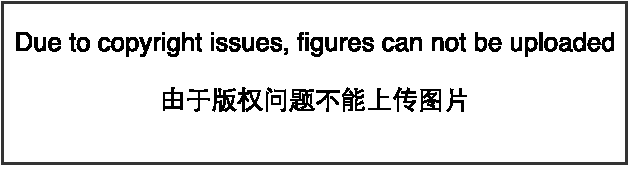
\includegraphics{figure.pdf}}
\else
\centerline{\includegraphics{Chapter7/figures/reg_l2}}
\fi
\caption{$L^2$(或\gls{weight_decay})\gls{regularization}对最佳$\Vw$值的影响。
实线椭圆表示没有\gls{regularization}目标的等值线。
虚线圆圈表示$L^2$正则化项的等值线。
在$\tilde{\Vw}$点,这两个竞争目标达到平衡。
目标函数$J$的~\gls{hessian}~的第一维特征值很小。
当从$\Vw^*$水平移动时,\gls{objective_function}不会增加得太多。
因为\gls{objective_function}对这个方向没有强烈的偏好,所以正则化项对该轴具有强烈的影响。
正则化项将$w_1$拉向零。
而\gls{objective_function}对沿着第二维远离$\Vw^*$的移动非常敏感。
对应的特征值较大,表示高\gls{curvature}。
因此,\gls{weight_decay}对$w_2$的位置影响相对较小。
}
\label{fig:chap7_reg_l2}
\end{figure}

% -- 225 --

只有在显著减小\gls{objective_function}方向上的参数会保留得相对完好。
在无助于\gls{objective_function}减小的方向(对应~\gls{hessian}~矩阵较小的特征值)上改变参数不会显著增加\gls{gradient}。
这种不重要方向对应的分量会在训练过程中因\gls{regularization}而衰减掉。


目前为止,我们讨论了\gls{weight_decay}对优化一个抽象通用的二次\gls{cost_function}的影响。
这些影响具体是怎么和机器学习关联的呢?
我们可以研究\gls{linear_regression},它的真实\gls{cost_function}是二次的,因此我们可以使用相同的方法分析。
再次应用分析,我们会在这种情况下得到相同的结果,但这次我们使用训练数据的术语表述。
\gls{linear_regression}的\gls{cost_function}是平方误差之和:
\begin{align}
 (\MX \Vw - \Vy)^\top (\MX \Vw - \Vy).
\end{align}
我们添加$L^2$正则项后,\gls{objective_function}变为
\begin{align}
  (\MX \Vw - \Vy)^\top (\MX \Vw - \Vy) + \frac{1}{2}\alpha \Vw^\top \Vw.
\end{align}
这将普通方程的解从
\begin{align}
\label{eq:716w}
  \Vw = (\MX^\top \MX)^{-1} \MX^\top \Vy
\end{align}
变为
\begin{align}
\label{eq:717mw}
   \Vw = (\MX^\top \MX + \alpha \MI)^{-1} \MX^\top \Vy .
\end{align}
\eqnref{eq:716w}中的矩阵$\MX^\top\MX$与\gls{covariance}矩阵$\frac{1}{m}\MX^\top\MX$成正比。
$L^2$正则项将这个矩阵替换为\eqnref{eq:717mw}中的$ (\MX^\top \MX + \alpha \MI)^{-1}$
这个新矩阵与原来的是一样的,不同的仅仅是在对角加了$\alpha$。
这个矩阵的对角项对应每个输入特征的\gls{variance}。
我们可以看到,$L^2$\gls{regularization}能让学习算法``感知''到具有较高方差的输入$\Vx$,因此与输出目标的\gls{covariance}较小(相对增加方差)的特征的权重将会收缩。

\subsection{$L^1$参数\glsentrytext{regularization}}
\label{sec:l1_regularization}
$L^2$\gls{weight_decay}是\gls{weight_decay}最常见的形式,我们还可以使用其他的方法限制模型参数的大小。
比如我们还可以使用$L^1$\gls{regularization}。

形式地,对模型参数$\Vw$的$L^1$\gls{regularization}被定义为:
\begin{align}
 \Omega(\Vtheta) = \norm{ \Vw }_1 = \sum_i | w_i |,
 \end{align}
即各个参数的绝对值之和\footnote{如同$L^2$\gls{regularization},我们能将参数\gls{regularization}到其他非零值$\Vw^{(o)}$。在这种情况下,$L^1$\gls{regularization}将会引入不同的项$\Omega(\Vtheta)=
\|\Vw - \Vw^{(o)} \|_1 = \sum_i | w_i - w_i^{(o)} |$。}。
接着我们将讨论$L^1$\gls{regularization}对简单\gls{linear_regression}模型的影响,与分析$L^2$\gls{regularization}时一样不考虑\gls{bias_aff}参数。  
我们尤其感兴趣的是找出$L^1$和$L^2$\gls{regularization}之间的差异。
与$L^2$\gls{weight_decay}类似,我们也可以通过缩放惩罚项$\Omega$的正超参数$\alpha$来控制$L^1$\gls{weight_decay}的强度。 
因此,\gls{regularization}的\gls{objective_function} $\tilde{J}(\Vw;\MX, \Vy)$如下所示
\begin{align}
\tilde{J}(\Vw;\MX, \Vy) = \alpha \| \Vw \|_1 +  J(\Vw;\MX, \Vy) ,
\end{align}
对应的梯度(实际上是次梯度):
\begin{align}
\label{eq:subgradient}
  \nabla_{\Vw} \tilde{J}(\Vw; \MX, \Vy) = \alpha \text{sign}(\Vw) + \nabla_{\Vw} J(\Vw; \MX, \Vy), % ?? may be wrong
\end{align}
其中$\text{sign}(\Vw)$只是简单地取$\Vw$各个元素的正负号。

% -- 227 --

观察\eqnref{eq:subgradient},我们立刻发现$L^1$的\gls{regularization}效果与$L^2$大不一样。
具体来说,我们可以看到\gls{regularization}对\gls{gradient}的影响不再是线性地缩放每个$w_i$;而是添加了一项与$\text{sign}(w_i)$同号的常数。
使用这种形式的\gls{gradient}之后,我们不一定能得到$J(\MX, \Vy;\Vw)$二次近似的直接算术解($L^2$\gls{regularization}时可以)。 
 
简单\gls{linear_model}具有二次\gls{cost_function},我们可以通过\gls{taylor}级数表示。
或者我们可以设想,这是逼近更复杂模型的\gls{cost_function}的截断\gls{taylor}级数。
在这个设定下,\gls{gradient}由下式给出
\begin{align}
  \nabla_{\Vw} \hat{J}(\Vw) = \MH (\Vw - \Vw^*),
\end{align}
同样,$\MH$是$J$在$\Vw^*$处的\gls{hessian}矩阵(关于$\Vw$)。

由于$L^1$惩罚项在满的、一般的~\gls{hessian}~的情况下,无法得到直接清晰的代数表达式,因此我们将进一步简化假设~\gls{hessian}~是对角的,即$\MH = \text{diag}([H_{1,1},\dots, H_{n,n}])$,其中每个$H_{i,i}>0$。
如果\gls{linear_regression}问题中的数据已被预处理(如可以使用PCA),去除了输入特征之间的相关性,那么这一假设成立。

我们可以将$L^1$\gls{regularization}目标函数的二次近似分解成关于参数的求和:
\begin{align}
 \hat J(\Vw; \MX, \Vy) = J(\Vw^*; \MX, \Vy) + \sum_i \Bigg [\frac{1}{2} H_{i,i} (w_i - w_i^*)^2 
 + \alpha |w_i| \Bigg].  % I think this is correct
\end{align}
如下列形式的解析解(对每一维$i$)可以最小化这个近似\gls{cost_function}:
\begin{align}
w_i = \text{sign}(w_i^*) \max\Big\{ |w_i^*| - \frac{\alpha}{H_{i,i}} , 0\Big\} .
\end{align}
考虑所有$i$且$w_i^* > 0$的情形,会有两种可能输出:
\begin{enumerate}
\item $w_i^* \leq \frac{\alpha}{H_{i,i}}$的情况。
\gls{regularization}后目标中的$w_i$最优值是$w_i = 0$。
这是因为在方向$i$上$J(\Vw; \MX, \Vy) $对$ \hat J(\Vw; \MX, \Vy)$的贡献受到抑制,$L^1$\gls{regularization}项将$w_i$推向0。
\item  $w_i^* > \frac{\alpha}{H_{i,i}}$的情况。在这种情况下,\gls{regularization}不会将$w_i$的最优值推向0,而仅仅在那个方向上移动$\frac{\alpha}{H_{i,i}}$的距离。
\end{enumerate}
$w_i^* < 0$的情况与之类似,但是$L^1$惩罚项使$w_i$更接近0(增加$ \frac{\alpha}{H_{i,i}}$)或者为0。

相比$L^2$\gls{regularization},$L^1$\gls{regularization}会产生更\firstgls{sparse}的解。
此处\gls{sparse}性指的是一些参数具有最优值0。
和$L^2$\gls{regularization}相比,$L^1$\gls{regularization}的\gls{sparse}性具有本质的不同。
\eqnref{eq:713L2}给出了$L^2$\gls{regularization}的解$\tilde \Vw$。 
如果我们使用~\gls{hessian}~矩阵$\MH$为对角正定矩阵的假设(与$L^1$\gls{regularization}分析时一样),重新考虑这个等式,我们发现
$\tilde{w_i} = \frac{H_{i,i}}{H_{i,i} + \alpha} w_i^*$。
如果$w_i^*$不是零,那么$\tilde{w_i}$也会保持非零。 
这表明$L^2$\gls{regularization}不会使参数变得\gls{sparse},而$L^1$\gls{regularization}有可能通过足够大的$\alpha$实现\gls{sparse}。
 
由$L^1$\gls{regularization}导出的\gls{sparse}性质已经被广泛地用于\firstgls{feature_selection}机制。
\gls{feature_selection}从可用的特征子集选择出有意义的特征,化简\gls{ML}问题。
著名的LASSO~\citep{Tibshirani95}(Least Absolute Shrinkage and
Selection Operator)模型将$L^1$惩罚和\gls{linear_model}结合,并使用最小二乘\gls{cost_function}。 
$L^1$惩罚使部分子集的权重为零,表明相应的特征可以被安全地忽略。
 
在\secref{sec:maximum_a_posteriori_map_estimation},我们看到许多\gls{regularization}策略可以被解释为~\glssymbol{MAP}~贝叶斯推断,
特别是$L^2$\gls{regularization}相当于权重是高斯先验的~\glssymbol{MAP}~贝叶斯推断。
对于$L^1$\gls{regularization},用于\gls{regularization}\gls{cost_function}的惩罚项$\alpha \Omega(\Vw) =  \alpha \sum_i |w_i |$与通过~\glssymbol{MAP}~贝叶斯推断最大化的对数先验项是等价的($\Vw \in \SetR^n$并且权重先验是各向同性的拉普拉斯分布(\eqnref{eq:chap3_laplace})):
\begin{align}
\log p(\Vw) = \sum_i \log \text{Laplace}(w_i;0,\frac{1}{\alpha}) = 
  -\alpha \norm{\Vw}_1 + n \log \alpha - n \log 2.
\end{align}
因为是关于$\Vw$最大化进行学习,我们可以忽略$\log \alpha - \log 2$项,因为它们与$\Vw$无关。
 
 % -- 229 --
 
 \section{作为约束的范数惩罚}
 \label{sec:7.2}
考虑通过参数范数\gls{regularization}的\gls{cost_function}:
\begin{align}
 \tilde{J}(\Vtheta;\MX, \Vy) = J(\Vtheta;\MX, \Vy) + \alpha \Omega(\Vtheta) .
\end{align}

回顾\secref{sec:constrained_optimization}我们可以构造一个\gls{generalized_lagrange_function}来最小化带约束的函数,即在原始\gls{objective_function}上添加一系列惩罚项。
每个惩罚是一个系数之间的乘积,被称为\firstgls{KKT}乘子,以及一个表示约束是否满足的函数。
如果我们想约束$\Omega(\Vtheta)$小于某个常数$k$,我们可以构建\gls{generalized_lagrange_function}
\begin{align}
 \CalL(\Vtheta, \alpha; \MX, \Vy) = J(\Vtheta; \MX, \Vy) + \alpha (\Omega(\Vtheta) - k).
\end{align}

这个约束问题的解由下式给出
\begin{align}
 \Vtheta^* = \underset{\Vtheta}{ \argmin} \underset{\alpha, \alpha \geq 0}{\max} \CalL(\Vtheta, \alpha).
\end{align}

如\secref{sec:constrained_optimization}中描述的,解决这个问题我们需要同时改变$\Vtheta$和$\alpha$。
\secref{sec:example_linear_least_squares}给出了一个带$L^2$约束的\gls{linear_regression}实例。
还有许多不同的优化方法,有些可能会使用\gls{GD}而其他可能会使用\gls{gradient}为0的解析解,但在所有程序中$\alpha$在$\Omega(\Vtheta) > k$时必须增加,在$\Omega(\Vtheta) < k$时必须减小。
所有正值的$\alpha$都鼓励$\Omega(\Vtheta)$收缩。
最优值$\alpha^*$也将鼓励$\Omega(\Vtheta)$收缩,但不会像$\Omega(\Vtheta)$小于$k$时那么强烈。

为了洞察约束的影响,我们可以固定$\alpha^*$,把这个问题看成只跟$\Vtheta$有关的函数:
\begin{align}
 \Vtheta^* =  \underset{\Vtheta}{ \argmin} ~\CalL(\Vtheta, \alpha^*) = 
 \underset{\Vtheta}{ \argmin}~
 J(\Vtheta; \MX, \Vy) + \alpha^* \Omega(\Vtheta).
\end{align}
这和最小化$\tilde J$的\gls{regularization}训练问题是完全一样的。
因此,我们可以把参数范数惩罚看作对权重强加的约束。
如果$\Omega$是$L^2$范数,那么权重就是被约束在一个$L^2$球中。
如果$\Omega$是$L^1$范数,那么权重就是被约束在一个$L^1$范数限制的区域中。
通常我们不知道\gls{weight_decay}系数$\alpha^*$约束的区域大小,因为$\alpha^*$的值不直接告诉我们$k$的值。
原则上我们可以解得$k$,但$k$和$\alpha^*$之间的关系取决于$J$的形式。
虽然我们不知道约束区域的确切大小,但我们可以通过增加或者减小$\alpha$来大致扩大或收缩约束区域。
较大的$\alpha$,将得到一个较小的约束区域。
较小的$\alpha$,将得到一个较大的约束区域。

% -- 230 --

有时候,我们希望使用显式的限制,而不是惩罚。
如\secref{sec:constrained_optimization}所述,我们可以修改下降算法(如\gls{SGD}算法),使其先计算$J(\Vtheta)$的下降步,然后将$\Vtheta$投影到满足$\Omega(\Vtheta) < k$的最近点。
如果我们知道什么样的$k$是合适的,而不想花时间寻找对应于此$k$处的$\alpha$值,这会非常有用。

另一个使用显式约束和重投影而不是使用惩罚强加约束的原因是惩罚可能会导致\gls{objective_function}非凸而使算法陷入局部极小(对应于小的$\Vtheta$)。
当训练\gls{NN}时,这通常表现为训练带有几个``死亡单元''的\gls{NN}。
这些单元不会对网络学到的函数有太大影响,因为进入或离开它们的权重都非常小。
当使用权重范数的惩罚训练时,即使可以通过增加权重以显著减少$J$,这些配置也可能是局部最优的。
因为重投影实现的显式约束不鼓励权重接近原点,所以在这些情况下效果更好。
通过重投影实现的显式约束只在权重变大并试图离开限制区域时产生作用。

最后,因为重投影的显式约束还对优化过程增加了一定的稳定性,所以这是另一个好处。
当使用较高的学习率时,很可能进入正反馈,即大的权重诱导大\gls{gradient},然后使得权重获得较大更新。
如果这些更新持续增加权重的大小,$\Vtheta$就会迅速增大,直到离原点很远而发生溢出。
重投影的显式约束可以防止这种反馈环引起权重无限制地持续增加。
\cite{Hinton-et-al-arxiv2012}建议结合使用约束和高学习速率,这样能更快地探索参数空间,并保持一定的稳定性。

% -- 231 --

\cite{Hinton-et-al-arxiv2012}尤其推荐由\cite{Srebro05}引入的策略:约束\gls{NN}层的权重矩阵每列的范数,而不是限制整个权重矩阵的~\ENNAME{Frobenius}~范数。
分别限制每一列的范数可以防止某一\gls{hidden_unit}有非常大的权重。
如果我们将此约束转换成~\ENNAME{Lagrange}~函数中的一个惩罚,这将与$L^2$ \gls{weight_decay}类似但每个\gls{hidden_unit}的权重都具有单独的~\glssymbol{KKT}~乘子。
每个~\glssymbol{KKT}~乘子分别会被动态更新,以使每个\gls{hidden_unit}服从约束。
在实践中,列范数的限制总是通过重投影的显式约束来实现。

\section{\glsentrytext{regularization}和欠约束问题}
\label{sec:regularization_and_under_constrained_problems}
在某些情况下,为了正确定义\gls{ML}问题,\gls{regularization}是必要的。
\gls{ML}中许多\gls{linear_model},包括\gls{linear_regression}和PCA,都依赖于求逆矩阵$\MX^\top\MX$。
只要$\MX^\top\MX$是奇异的,这些方法就会失效。
当数据生成分布在一些方向上确实没有差异时,或因为例子较少(即相对输入特征($\MX$的列)来说)而在一些方向上没有观察到\gls{variance}时,这个矩阵就是奇异的。
在这种情况下,\gls{regularization}的许多形式对应求逆$\MX^\top\MX + \alpha \MI$。
这个\gls{regularization}矩阵可以保证是可逆的。

相关矩阵可逆时,这些线性问题有\gls{closed_form_solution}。
没有\gls{closed_form_solution}的问题也可能是欠定的。
一个例子是应用于线性可分问题的\gls{logistic_regression}。
如果权重向量$\Vw$能够实现完美分类,那么$2 \Vw$也会以较高似然实现完美分类。
类似\gls{SGD}的迭代优化算法将持续增加$\Vw$的大小,理论上永远不会停止。
在实践中,数值实现的\gls{GD}最终会达到导致数值溢出的超大权重,此时的行为将取决于程序员如何处理这些不是真正数字的值。

大多数形式的\gls{regularization}能够保证应用于欠定问题的迭代方法收敛。
例如,当似然的斜率等于\gls{weight_decay}的系数时, \gls{weight_decay}将阻止\gls{GD}继续增加权重的大小。

使用\gls{regularization}解决欠定问题的想法超出了\gls{ML}的范畴。
同样的想法在几个基本线性代数问题中也非常有用。

% -- 232 --

正如我们在\secref{sec:the_moore_penrose_pseudoinverse}看到的,我们可以使用~\ENNAME{Moore-Penrose}~求解欠定线性方程。 
回想$\MX$伪逆$\MX^+$的一个定义:
\begin{align} 
\label{eq:729pseudo}
 \MX^+ = \lim_{\alpha \searrow 0} (\MX^\top \MX + \alpha \MI)^{-1}\MX^\top.
\end{align}
现在我们可以将\secref{eq:729pseudo}看作进行具有\gls{weight_decay}的\gls{linear_regression}。
具体来说,当\gls{regularization}系数趋向0时,\eqnref{eq:729pseudo}是\eqnref{eq:717mw}的极限。
因此,我们可以将伪逆解释为使用\gls{regularization}来稳定欠定问题。


\section{数据集增强}
\label{sec:dataset_augmentation_chap7}
让\gls{ML}模型泛化得更好的最好办法是使用更多的数据进行训练。
当然,在实践中,我们拥有的数据量是很有限的。
解决这个问题的一种方法是创建假数据并添加到训练集中。
对于一些\gls{ML}任务,创建新的假数据相当简单。

对分类来说这种方法是最简单的。
分类器需要一个复杂的高维输入$\Vx$,并用单个类别标识$y$概括$\Vx$。
这意味着分类面临的一个主要任务是要对各种各样的变换保持不变。
我们可以轻易通过转换训练集中的$\Vx$来生成新的$(\Vx, y)$对。

这种方法对于其他许多任务来说并不那么容易。
例如,除非我们已经解决了密度估计问题,否则在密度估计任务中生成新的假数据是很困难的。

数据集增强对一个具体的分类问题来说是特别有效的方法:对象识别。
图像是高维的并包括各种巨大的变化因素,其中有许多可以轻易地模拟。
即使模型已使用卷积和\gls{pooling}技术(\chapref{chap:convolutional_networks})对部分平移保持不变,沿训练图像每个方向平移几个像素的操作通常可以大大改善泛化。
许多其他操作如旋转图像或缩放图像也已被证明非常有效。

我们必须要小心,不能使用会改变类别的转换。
例如,光学字符识别任务需要认识到``b''和``d''以及``6''和``9''的区别,所以对这些任务来说,水平翻转和旋转$180^{\circ}$并不是合适的数据集增强方式。

% -- 233 --

能保持我们希望的分类不变,但不容易执行的转换也是存在的。
例如,平面外绕轴转动难以通过简单的几何运算在输入像素上实现。

数据集增强对语音识别任务也是有效的\citep{Jaitly_VTLP_2013}。

在\gls{NN}的输入层注入噪声\citep{SietsmaDow91}也可以被看作是数据增强的一种方式。
对于许多分类甚至一些回归任务而言,即使小的随机噪声被加到输入,任务仍应该是能够被解决的。
然而 ,\gls{NN}被证明对噪声不是非常健壮\citep{TangElias10}。
改善\gls{NN}健壮性的方法之一是简单地将随机噪声添加到输入再进行训练。
输入噪声注入是一些\gls{unsupervised_learning}算法的一部分,如\gls{DAE}\citep{VincentPLarochelleH2008}。
向\gls{hidden_unit}施加噪声也是可行的,这可以被看作在多个抽象层上进行的数据集增强。
\cite{Poole14}最近表明,噪声的幅度被细心调整后,该方法是非常高效的。
我们将在\secref{sec:dropout}介绍一个强大的\gls{regularization}策略~\gls{dropout},该策略可以被看作是通过与噪声\emph{相乘}构建新输入的过程。

在比较\gls{ML}基准测试的结果时,考虑其采取的数据集增强是很重要的。
通常情况下,人工设计的数据集增强方案可以大大减少\gls{ML}技术的泛化误差。
将一个\gls{ML}算法的性能与另一个进行对比时,对照实验是必要的。
在比较\gls{ML}算法A和\gls{ML}算法B时,应该确保这两个算法使用同一人工设计的数据集增强方案进行评估。
假设算法$A$在没有数据集增强时表现不佳,而$B$结合大量人工转换的数据后表现良好。
在这样的情况下,很可能是合成转化引起了性能改进,而不是\gls{ML}算法$B$比算法$A$更好。 
有时候,确定实验是否已经适当控制需要主观判断。
例如,向输入注入噪声的\gls{ML}算法是执行数据集增强的一种形式。
通常,普适操作(例如,向输入添加高斯噪声)被认为是\gls{ML}算法的一部分,
而特定于一个应用领域(如随机地裁剪图像)的操作被认为是独立的预处理步骤。

% -- 234 --

\section{噪声鲁棒性}
\label{sec:noise_robustness}

\secref{sec:dataset_augmentation_chap7}已经提出将噪声作用于输入,作为数据集增强策略。
对于某些模型而言,向输入添加方差极小的噪声等价于对权重施加范数惩罚\citep{Bishop1995,bishop95training}。
在一般情况下,噪声注入远比简单地收缩参数强大,特别是噪声被添加到\gls{hidden_unit}时会更加强大。
向\gls{hidden_unit}添加噪声是值得单独讨论重要的话题;在\secref{sec:dropout}所述~\gls{dropout}~算法是这种做法的主要发展方向。

另一种\gls{regularization}模型的噪声使用方式是将其加到的权重。
这项技术主要用于\gls{RNN}~\citep{JimGilesHorne1996,Graves-2011}。
这可以被解释为关于权重的贝叶斯\gls{inference}的随机实现。
贝叶斯学习过程将权重视为不确定的,并且可以通过概率分布表示这种不确定性。
向权重添加噪声是反映这种不确定性的一种实用的随机方法。

在某些假设下,施加于权重的噪声可以被解释为与更传统的\gls{regularization}形式等同,鼓励要学习的函数保持稳定。
我们研究回归的情形,也就是训练将一组特征$\Vx$映射成一个标量的函数$\hat y(\Vx)$,并使用最小二乘\gls{cost_function}衡量模型预测值$\hat y(\Vx)$与真实值$y$的误差:
\begin{align}
 J = \SetE_{p(x,y)}[(\hat y(\Vx) - y)^2].
\end{align}
训练集包含$m$对标注样例$\{(\Vx^{(1)}, y^{(1)}),\dots,(\Vx^{(m)}, y^{(m)})\}$。

现在我们假设对每个输入表示,网络权重添加随机扰动$\epsilon_{\Vw} \sim \CalN(\Vepsilon;0, \eta\MI \, )$。
想象我们有一个标准的$l$层MLP。
我们将扰动模型记为$\hat y_{\epsilon_{\MW}} (\Vx)$。
尽管有噪声注入,我们仍然希望减少网络输出误差的平方。
因此目标函数变为:
\begin{align}
 \tilde J_{\MW} &= \SetE_{p(\Vx,y,\epsilon_{\MW})}[(\hat y_{\epsilon_{\MW}}(\Vx) - y)^2] \\
   &=  \SetE_{p(\Vx,y,\epsilon_{\MW})}[\hat y_{\epsilon_{\MW}}^2(\Vx) -  2y\hat y_{\epsilon_{\MW}}
   (\Vx)+ y^2] .
\end{align}

对于小的$\eta$,最小化带权重噪声(方差为$\eta \MI$\,)的$J$等同于最小化附加\gls{regularization}项的$J$:
$ \eta \SetE_{p(\Vx,y)}[\norm{\nabla_{\MW}~\hat y(\Vx)}^2]$。
这种形式的\gls{regularization}鼓励参数进入权重小扰动对输出相对影响较小的参数空间区域。
换句话说,它推动模型进入对权重小的变化相对不敏感的区域,找到的点不只是极小点,还是由平坦区域所包围的最小点\citep{Hochreiter95}。
在简化的线性回归中(例如,$\hat y(\Vx) = \Vw^\top \Vx + b$),正则项退化为$ \eta \SetE_{p(\Vx)}[\norm{\Vx}^2]$,这与函数的参数无关,因此不会对$\tilde J_{\Vw}$关于模型参数的梯度有影响。

% -- 235 --

\subsection{向输出目标注入噪声}
\label{sec:injecting_noise_at_the_output_targets}
大多数数据集的$y$标签都有一定错误。
错误的$y$不利于最大化$\log p(y \mid \Vx)$。
避免这种情况的一种方法是显式地对标签上的噪声进行建模。
例如,我们可以假设,对于一些小常数$\epsilon$,训练集标记$y$是正确的概率是$1-\epsilon$,(以$\epsilon$的概率)任何其他可能的标签可能是正确的。
这个假设很容易就能解析地与\gls{cost_function}结合,而不用显式地抽取噪声样本。
例如,\textbf{标签平滑}(label smoothing)通过把确切分类目标从0和1替换成$\frac{\epsilon}{k-1}$和$1-\epsilon$,\gls{regularization}具有$k$个输出的~\gls{softmax}~的模型。
标准交叉熵损失可以用在这些非确切目标的输出上。
使用~\gls{softmax}~和明确目标的最大似然学习可能永远不会收敛——
\gls{softmax}~永远无法真正预测0概率或1概率,因此它会继续学习越来越大的权重,使预测更极端。
使用如\gls{weight_decay}等其他\gls{regularization}策略能够防止这种情况。
标签平滑的优势是能够防止模型追求确切概率而不影响模型学习正确分类。
这种策略自20世纪80年代就已经被使用,并在现代神经网络继续保持显著特色\citep{Szegedy-et-al-2015}。

% -- 236 --

\section{\glsentrytext{semi_supervised_learning}}
\label{sec:semi_supervised_learning}
在\gls{semi_supervised_learning}的框架下,$P(\RVx)$产生的未标记样本和$P(\RVx, \RVy)$中的标记样本都用于估计$P(\RVy \mid \RVx)$或者根据$\RVx$预测$\RVy$。

在\gls{DL}的背景下,\gls{semi_supervised_learning}通常指的是学习一个\gls{representation} $h = f(\Vx)$。 
学习\gls{representation}的目的是使相同类中的\gls{example}有类似的表示。
\gls{unsupervised_learning}可以为如何在\gls{representation}空间聚集\gls{example}提供有用线索。
在输入空间紧密聚集的\gls{example}应该被映射到类似的表示。
在许多情况下,新空间上的线性分类器可以达到较好的泛化\citep{Belkin+Niyogi-2002,Chapelle+al-2003}。
这种方法的一个经典变种是使用主成分分析\gls{PCA}作为分类前(在投影后的数据上分类)的预处理步骤。

我们可以构建这样一个模型,其中生成模型$P(\RVx)$或$P(\RVx, \RVy)$与判别模型$P(\RVy \mid \RVx)$共享参数,而不用分离\gls{unsupervised}和\gls{supervised}部分。
我们权衡\gls{supervised}模型\gls{criterion} $-\log P(\RVy \mid \RVx)$和\gls{unsupervised}或生成模型\gls{criterion}(如$-\log P(\RVx)$或$-\log P(\RVx, \RVy)$)。
生成模型\gls{criterion}表达了对\gls{supervised_learning}问题解的特殊形式的先验知识\citep{LasserreJ2006},即$P(\RVx)$的结构通过某种共享参数的方式连接到$P(\RVy \mid \RVx)$。
通过控制在总\gls{criterion}中的生成\gls{criterion},我们可以获得比纯生成或纯判别训练\gls{criterion}更好的权衡\citep{LasserreJ2006,Larochelle2008}。

\cite{Russ+Geoff-nips-2007}描述了一种学习回归\gls{kernel_machines}中核函数的方法,其中建模$P(\RVx)$时使用的未标记样本大大提高了$P(\RVy \mid \RVx)$的效果。

更多\gls{semi_supervised_learning}的信息,请参阅~\cite{SSL-Book-2006}。

\section{\glsentrytext{multitask_learning}}
\label{sec:multitask_learning}
\gls{multitask_learning}~\citep{caruana93a}是通过合并几个任务中的样例(可以视为对参数施加的软约束)来提高泛化的一种方式。
额外的训练样本以同样的方式将模型的参数推向泛化更好的方向,当模型的一部分在任务之间共享时,模型的这一部分更多地被约束为良好的值(假设共享是合理的),往往能更好地泛化。

\figref{fig:chap7_multi_factor_output}展示了\gls{multitask_learning}中非常普遍的一种形式,其中不同的\gls{supervised}任务(给定$\RVx$预测$\RVy^{(i)}$)共享相同的输入$\RVx$以及一些中间层表示$\Vh^{(\text{share})}$,能学习共同的因素池。
该模型通常可以分为两类相关的参数:
\begin{enumerate}
 \item 具体任务的参数 (只能从各自任务的样本中实现良好的泛化)。如\figref{fig:chap7_multi_factor_output}中的上层。
 \item 所有任务共享的通用参数(从所有任务的汇集数据中获益)。如\figref{fig:chap7_multi_factor_output}中的下层。
\end{enumerate}
\begin{figure}[!htb]
\ifOpenSource
\centerline{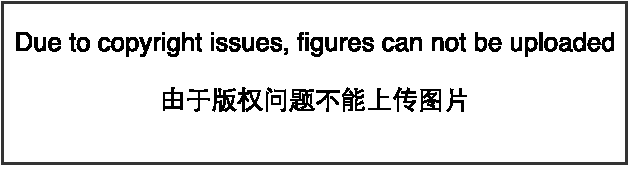
\includegraphics{figure.pdf}}
\else
\centerline{\includegraphics{Chapter7/figures/multi_factor_output}}
\fi
\caption{\gls{multitask_learning}在深度学习框架中可以以多种方式进行,该图说明了任务共享相同输入但涉及不同目标随机变量的常见情况。
\gls{deep_network}的较低层(无论是\gls{supervised}前馈的,还是包括向下箭头的生成组件)可以跨这样的任务共享,而任务特定的参数(分别与从$\Vh^{(1)}$和$\Vh^{(2)}$进入和发出的权重)可以在共享表示$\Vh^{(\text{shared})}$之上学习。
这里的基本假设是存在解释输入$\RVx$变化的共同因素池,而每个任务与这些因素的子集相关联。
在该示例中,额外假设顶层\gls{hidden_unit} $\Vh^{(1)}$和$\Vh^{(2)}$专用于每个任务(分别预测$\RVy^{(1)}$和$\RVy^{(2)}$),而一些中间层表示$\Vh^{(\text{shared})}$在所有任务之间共享。
在\gls{unsupervised_learning}情况下,一些顶层因素不与输出任务$(\Vh^{(3)})$的任意一个关联是有意义的:这些因素可以解释一些输入变化但与预测$\RVy^{(1)}$或$\RVy^{(2)}$不相关。
}
\label{fig:chap7_multi_factor_output}
\end{figure}

因为共享参数,其统计强度可大大提高(共享参数的样本数量相对于单任务模式增加的比例),并能改善泛化和泛化误差的范围\citep{baxter95a}。
当然,仅当不同的任务之间存在某些统计关系的假设是合理(意味着某些参数能通过不同任务共享)时才会发生这种情况。

从\gls{DL}的观点看,底层的先验知识如下:\emph{能解释数据变化(在与之相关联的不同任务中观察到)的因素中,某些因素是跨两个或更多任务共享的。}

% -- 238 --

\section{\glsentrytext{early_stopping}}
\label{sec:early_stopping}
当训练有足够的表示能力甚至会过拟合任务的大模型时,我们经常观察到,训练误差会随着时间的推移逐渐降低但验证集的误差会再次上升。
\figref{fig:chap7_learning_curve}是这些现象的一个例子,这种现象几乎一定会出现。

这意味着如果我们返回使验证集误差最低的参数设置,就可以获得更好的模型(因此,有希望获得更好的测试误差)。
在每次验证集误差有所改善后,我们存储模型参数的副本。
当训练算法终止时,我们返回这些参数而不是最新的参数。
当验证集上的误差在事先指定的循环次数内没有进一步改善时,算法就会终止。
此过程在\algref{alg:early_stopping}中有更正式的说明。


% -- 239 --

这种策略被称为\firstgls{early_stopping}。
这可能是\gls{DL}中最常用的\gls{regularization}形式。
它的流行主要是因为有效性和简单性。

\begin{algorithm}[ht]
\caption{用于确定最佳训练时间量的\gls{early_stopping}元算法。
这种元算法是一种通用策略,可以很好地在各种训练算法和各种量化验证集误差的方法上工作。
}
\label{alg:early_stopping}
\begin{algorithmic}
\STATE 令 $n$ 为评估间隔的步数。
\STATE 令 $p$ 为 ``耐心(patience)'',即观察到较坏的验证集表现$p$次后终止。 
\STATE 令 $\Vtheta_{o}$ 为初始参数。
\STATE $\Vtheta \leftarrow \Vtheta_{o}$
\STATE $i \leftarrow 0$
\STATE $j \leftarrow 0$
\STATE $v \leftarrow \infty$
\STATE $\Vtheta^* \leftarrow \Vtheta$
\STATE $i^* \leftarrow i$
\WHILE{$j < p$}
    \STATE 运行训练算法$n$步,更新 $\Vtheta$ 。
    \STATE $i \leftarrow i + n$
    \STATE $v' \leftarrow \text{ValidationSetError}(\Vtheta)$
    \IF{$v' < v$}
        \STATE $j \leftarrow 0$
        \STATE $\Vtheta^* \leftarrow \Vtheta$
        \STATE $i^* \leftarrow i$
        \STATE $v \leftarrow v'$
    \ELSE
        \STATE $j \leftarrow j + 1$
    \ENDIF
\ENDWHILE
% pdflatex told me \RETURN was not recognized, wtf
\STATE 最佳参数为 $\Vtheta^*$,最佳训练步数为$i^*$
\end{algorithmic}
\end{algorithm}


我们可以认为\gls{early_stopping}是非常高效的超参数选择算法。
按照这种观点,训练步数仅是另一个超参数。
我们从\figref{fig:chap7_learning_curve}可以看到,这个超参数在验证集上具有U型性能曲线。
很多控制模型容量的超参数在验证集上都是这样的U型性能曲线,如\figref{fig:chap7_learning_curve}。
在\gls{early_stopping}的情况下,我们通过拟合训练集的步数来控制模型的有效容量。
大多数超参数的选择必须使用高代价的猜测和检查过程,我们需要在训练开始时猜测一个超参数,然后运行几个步骤检查它的训练效果。
``训练时间''是唯一只要跑一次训练就能尝试很多值的超参数。
通过\gls{early_stopping}自动选择超参数的唯一显著的代价是训练期间要定期评估验证集。
在理想情况下,这可以并行在与主训练过程分离的机器上,或独立的CPU,或独立的GPU上完成。
如果没有这些额外的资源,可以使用比训练集小的验证集或较不频繁地评估验证集来减小评估代价,较粗略地估算取得最佳的训练时间。

另一个\gls{early_stopping}的额外代价是需要保持最佳的参数副本。
这种代价一般是可忽略的,因为可以将它储存在较慢较大的存储器上(例如,在GPU内存中训练,但将最佳参数存储在主存储器或磁盘驱动器上)。
由于最佳参数的写入很少发生而且从不在训练过程中读取,这些偶发的慢写入对总训练时间的影响不大。

\begin{figure}[!htb]
\ifOpenSource
\centerline{\includegraphics{figure.pdf}}
\else
\centerline{\includegraphics{Chapter7/figures/learning_curve_color}}
\fi
\caption{学习曲线显示负对数似然损失如何随时间变化(表示为遍历数据集的训练迭代数,或\firstgls{epochs})。
在这个例子中,我们在MNIST上训练了一个~\gls{maxout}~网络。
我们可以观察到训练目标随时间持续减小,但验证集上的平均损失最终会再次增加,形成不对称的U形曲线。
}
\label{fig:chap7_learning_curve}
\end{figure}

% -- 240 --

\gls{early_stopping}是一种非常不显眼的\gls{regularization}形式,它几乎不需要改变基本训练过程、\gls{objective_function}或一组允许的参数值。
这意味着,无需破坏学习动态就能很容易地使用\gls{early_stopping}。
相对于\gls{weight_decay},必须小心不能使用太多的\gls{weight_decay},以防网络陷入不良\gls{local_minimum}(对应于病态的小权重)。

\gls{early_stopping}可单独使用或与其他的\gls{regularization}策略结合使用。
即使为鼓励更好泛化,使用\gls{regularization}策略改进\gls{objective_function},在训练目标的\gls{local_minimum}达到最好泛化也是非常罕见的。

\gls{early_stopping}需要验证集,这意味着某些训练数据不能被馈送到模型。
为了更好地利用这一额外的数据,我们可以在完成\gls{early_stopping}的首次训练之后,进行额外的训练。
在第二轮额外的训练步骤中,所有的训练数据都被包括在内。
有两个基本的策略都可以用于第二轮训练过程。

% -- 241 --

一个策略(\algref{alg:early_stopping_retrain})是再次初始化模型,然后使用所有数据再次训练。
在这个第二轮训练过程中,我们使用第一轮\gls{early_stopping}训练确定的最佳步数。
此过程有一些细微之处。
例如,我们没有办法知道重新训练时,对参数进行相同次数的更新和对数据集进行相同的遍数哪一个更好。
由于训练集变大了,在第二轮训练时,每一次遍历数据集将会更多次地更新参数。

另一个策略是保持从第一轮训练获得的参数,然后使用全部的数据\emph{继续}训练。
在这个阶段,已经没有验证集指导我们需要在训练多少步后终止。
相反,我们可以监控验证集的平均损失函数,并继续训练,直到它低于\gls{early_stopping}过程终止时的目标值。
此策略避免了重新训练模型的高成本,但表现并没有那么好。
例如,验证集的目标不一定能达到之前的目标值,所以这种策略甚至不能保证终止。
我们会在\algref{alg:early_stopping_continue}中更正式地介绍这个过程。

\gls{early_stopping}对减少训练过程的计算成本也是有用的。
除了由于限制训练的迭代次数而明显减少的计算成本,还带来了\gls{regularization}的益处(不需要添加惩罚项的\gls{cost_function}或计算这种附加项的\gls{gradient})。

\begin{algorithm}[ht]
\caption{使用\gls{early_stopping}确定训练步数,然后在所有数据上训练的元算法。
}
\label{alg:early_stopping_retrain}
\begin{algorithmic}
\STATE 令 $\MX^{(\text{train})}$ 和 $\Vy^{(\text{train})}$ 为训练集。
\STATE 将 $\MX^{(\text{train})}$ 和 $\Vy^{(\text{train})}$ 分别分割为 $(\MX^{(\text{subtrain})}$, $\MX^{(\text{valid})})$ 和 $(\Vy^{(\text{subtrain})}$, $\Vy^{(\text{valid})})$。
\STATE 从随机 $\Vtheta$开始,使用$\MX^{(\text{subtrain})}$ 和 $\Vy^{(\text{subtrain})}$作为训练集,$\MX^{(\text{valid})}$ 和 $\Vy^{(\text{valid})}$ 作为验证集,运行 (\algref{alg:early_stopping})。这将返回最佳训练步数$i^*$。
\STATE 将 $\Vtheta$ 再次设为随机值。
\STATE 在 $\MX^{(\text{train})}$ 和 $\Vy^{(\text{train})}$ 上训练 $i^*$ 步。  
\end{algorithmic}
\end{algorithm}

\begin{algorithm}[ht]
\caption{
使用\gls{early_stopping}确定将会\gls{overfitting}的目标值,然后在所有数据上训练直到再次
达到该值的元算法。
}
\label{alg:early_stopping_continue}
\begin{algorithmic}
\STATE 令 $\MX^{(\text{train})}$ 和 $\Vy^{(\text{train})}$ 为训练集。
\STATE 将 $\MX^{(\text{train})}$ 和 $\Vy^{(\text{train})}$ 分别分割为 $(\MX^{(\text{subtrain})}$, $\MX^{(\text{valid})})$ 和 $(\Vy^{(\text{subtrain})}$, $\Vy^{(\text{valid})})$。
\STATE 从随机 $\Vtheta$开始,使用$\MX^{(\text{subtrain})}$ 和 $\Vy^{(\text{subtrain})}$作为训练集,$\MX^{(\text{valid})}$ 和 $\Vy^{(\text{valid})}$ 作为验证集,运行 (\algref{alg:early_stopping})。这会更新$\Vtheta$。
\STATE $\epsilon \leftarrow J(\Vtheta, \MX^{(\text{subtrain})},\Vy^{(\text{subtrain})})$
\WHILE{$J(\Vtheta, \MX^{(\text{valid})}, \Vy^{(\text{valid})}) > \epsilon$}
\STATE 在 $\MX^{(\text{train})}$ 和 $\Vy^{(\text{train})}$ 上训练 $n$ 步。  
\ENDWHILE
\end{algorithmic}
\end{algorithm}


% -- 242 --

\paragraph{\gls{early_stopping}为何具有\gls{regularization}效果:}
目前为止,我们已经声明\gls{early_stopping}是一种\gls{regularization}策略,但我们只通过展示验证集误差的学习曲线是一个U型曲线来支持这种说法。
\gls{early_stopping}\gls{regularization}模型的真正机制是什么呢? 
\cite{Bishop1995}和~\cite{Sjoberg95}认为\gls{early_stopping}可以将优化过程的参数空间限制在初始参数值$\Vtheta_0$的小邻域内。
更具体地,想象用学习率$\epsilon$进行$\tau$个优化步骤(对应于$\tau$个训练迭代)。
我们可以将$\epsilon \tau$作为有效\gls{capacity}的度量。
假设\gls{gradient}有界,限制迭代的次数和学习速率能够限制从$\Vtheta_0$到达的参数空间的大小,如\figref{fig:chap7_reg_l1_vs_l2_mistake}所示。
在这个意义上,$\epsilon \tau$的效果就好像是\gls{weight_decay}系数的倒数。

\begin{figure}[!htb]
\ifOpenSource
\centerline{\includegraphics{figure.pdf}}
\else
\centerline{\includegraphics[width=0.8\textwidth]{Chapter7/figures/reg_l1_vs_l2_mistake}}
\fi
\caption{\gls{early_stopping}效果的示意图。
\emph{(左)}实线轮廓线表示负对数似然的轮廓。
虚线表示从原点开始的~\glssymbol{SGD}~所经过的轨迹。 % ??
\gls{early_stopping}的轨迹在较早的点$\tilde \Vw$处停止,而不是停止在最小化代价的点$\Vw^*$处。
\emph{(右)}为了对比,使用$L^2$\gls{regularization}效果的示意图。
虚线圆圈表示$L^2$惩罚的轮廓,$L^2$惩罚使得总代价的最小值比非\gls{regularization}代价的最小值更靠近原点。
}
\label{fig:chap7_reg_l1_vs_l2_mistake}
\end{figure}

事实上,在二次误差的简单\gls{linear_model}和简单的\gls{GD}情况下,我们可以展示\gls{early_stopping}相当于$L^2$\gls{regularization}。

为了与经典$L^2$\gls{regularization}比较,我们只考察唯一的参数是线性权重($\Vtheta = \Vw$)的简单情形。
我们在权重$\Vw$的经验最佳值$\Vw^*$附近以二次近似建模\gls{cost_function} $J$:
\begin{align}
 \hat J(\Vtheta) = J(\Vw^*) + \frac{1}{2}  (\Vw- \Vw^*)^\top \MH  (\Vw - \Vw^*),
\end{align}
其中$\MH$是$J$关于$\Vw$在$\Vw^*$点的\gls{hessian}。
鉴于假设$\Vw^*$是$J(\Vw)$的最小点,我们知道$\MH$为半正定。
在局部\gls{taylor}级数逼近下,\gls{gradient}由下式给出:
\begin{align}
 \nabla_{\Vw} \hat J (\Vw) = \MH (\Vw - \Vw^*).
\end{align}

% -- 243 --

接下来我们研究训练时参数向量的轨迹。
为简化起见,我们将参数向量初始化为原点\footnote{对于\gls{NN},我们需要打破\gls{hidden_unit}间的对称平衡因此不能将所有参数都初始化为$\mathbf{0}$(如\secref{sec:gradient_based_learning}所讨论的)。
然而,对于其他任何初始值$\Vw_{(0)}$该论证都成立},也就是$\Vw^{(0)} = 0$。
我们通过分析$\hat{J}$上的\gls{GD}来研究$J$上近似的\gls{GD}的效果:
\begin{align}
\Vw^{(\tau)} &= \Vw^{(\tau-1)} -\epsilon \nabla_{\Vw} \hat{J}( \Vw^{(\tau-1)} ) \\
&=  \Vw^{(\tau-1)}  - \epsilon  \MH ( \Vw^{(\tau-1)} -  \Vw^* ), \\
\Vw^{(\tau)}  -  \Vw^* &= (\MI - \epsilon  \MH) ( \Vw^{(\tau-1)} -  \Vw^* ).
 \end{align}
现在让我们在$\MH$特征向量的空间中改写表达式,利用$\MH$的特征分解:$\MH = \MQ \VLambda \MQ^\top$,其中$\VLambda$是对角矩阵,$\MQ$是特征向量的一组标准正交基。
\begin{align}
\Vw^{(\tau)}  -  \Vw^* &= (\MI - \epsilon \MQ \VLambda \MQ^\top) ( \Vw^{(\tau-1)} -  \Vw^* ) \\
\MQ^\top (\Vw^{(\tau)}  -  \Vw^*) &= (\MI - \epsilon \VLambda)\MQ^\top ( \Vw^{(\tau-1)} -  \Vw^* )
\end{align}
假定$\Vw^{(0)} = 0$并且$\epsilon$选择得足够小以保证$|1 - \epsilon \lambda_i |<1$,经过$\tau$次参数更新后轨迹如下:
\begin{align} \label{eq:740qw}
\MQ^\top  \Vw^{(\tau)} = [\MI - (\MI - \epsilon \VLambda)^\tau] \MQ^\top  \Vw^* .
\end{align}
现在,\eqnref{eq:713L2}中$\MQ^\top \tilde \Vw$的表达式能被重写为:
\begin{align}
\MQ^\top  \tilde \Vw &= (\VLambda + \alpha \MI)^{-1} \VLambda \MQ^\top  \Vw^*, \\
\MQ^\top  \tilde \Vw &= [\MI - (\VLambda + \alpha \MI)^{-1} \alpha] \MQ^\top  \Vw^*. 
\label{eq:742qw}
\end{align}
比较\eqnref{eq:740qw}和\eqnref{eq:742qw},我们能够发现,如果超参数$\epsilon,\alpha$和$\tau$满足如下:
\begin{align}
(\MI - \epsilon \VLambda)^\tau =  (\VLambda + \alpha \MI)^{-1} \alpha,
\end{align}
那么$L^2~$\gls{regularization}和\gls{weight_decay}可以被看作是等价的(至少在\gls{objective_function}的二次近似下)。
进一步取对数,使用$\log~(1+x)$的级数展开,我们可以得出结论:如果所有$\lambda_i$是小的(即$\epsilon \lambda_i \ll 1$且$\lambda_i / \alpha \ll 1$),那么
\begin{align}
\tau \approx \frac{1}{\epsilon \alpha}, \\
\alpha \approx \frac{1}{\tau \epsilon}.
\end{align}
也就是说,在这些假设下,训练迭代次数$\tau$起着与$L^2$参数成反比的作用,$\tau \epsilon$的倒数与\gls{weight_decay}系数的作用类似。

对应显著曲率(\gls{objective_function})方向的参数值\gls{regularization}小于小曲率方向。
当然,在\gls{early_stopping}的情况下,这实际上意味着对应于显著曲率方向的参数比较小的曲率方向的参数更早地停止学习。
 
本节中的推导表明长度为$\tau$的轨迹结束于$L^2$\gls{regularization}目标的极小点。
当然,\gls{early_stopping}比简单的轨迹长度限制更丰富;相反,\gls{early_stopping}通常涉及监控验证集误差,以便在空间特别好的点处终止轨迹。
因此\gls{early_stopping}比\gls{weight_decay}更具有优势,\gls{early_stopping}能自动确定\gls{regularization}的正确量,而\gls{weight_decay}需要多个训练实验测试其超参数的不同值。

% -- 245 --

\section{参数绑定和参数共享}
\label{sec:parameter_tying_and_parameter_sharing}
目前为止,本章讨论对参数添加约束或惩罚时,一直是相对于固定的区域或点。
例如,$L^2$\gls{regularization}(或\gls{weight_decay})对参数偏离零的固定值进行惩罚。
然而,有时我们可能需要其他的方式来表达我们对模型参数适当值的先验知识。
有时候,我们可能无法准确地知道应该使用什么样的参数,但我们根据领域和模型结构方面的知识得知模型参数之间应该存在一些相关性。

我们经常想要表达的一种常见依赖是某些参数应当彼此接近。
考虑以下情形:我们有两个模型执行相同的分类任务(具有相同类别),但输入分布稍有不同。
形式地,我们有参数为$\Vw^{(A)}$的模型$A$和参数为$\Vw^{(B)}$的模型$B$。
这两种模型将输入映射到两个不同但相关的输出:$\hat y^{(A)} = f(\Vw^{(A)}, \Vx)$和$\hat y^{(B)} = f(\Vw^{(B)}, \Vx)$。

我们可以想象,这些任务会足够相似(或许具有相似的输入和输出分布),因此我们认为模型参数应彼此靠近:
$\forall i, w_i^{(A)}$应该与$ w_i^{(B)}$接近。
我们可以通过\gls{regularization}利用此信息。
具体来说,我们可以使用以下形式的参数范数惩罚:
$\Omega(\Vw^{(A)}, \Vw^{(B)}) = \norm{\Vw^{(A)}-\Vw^{(B)}}_2^2$。
在这里我们使用$L^2$惩罚,但也可以使用其他选择。

这种方法由\cite{LasserreJ2006}提出,\gls{regularization}一个模型(\gls{supervised}模式下训练的分类器)的参数,使其接近另一个\gls{unsupervised}模式下训练的模型(捕捉观察到的输入数据的分布)的参数。
这种构造架构使得许多分类模型中的参数能与之对应的\gls{unsupervised}模型的参数匹配。

参数范数惩罚是\gls{regularization}参数使其彼此接近的一种方式,而更流行的方法是使用约束:\emph{强迫某些参数相等}。
由于我们将各种模型或模型组件解释为共享唯一的一组参数,这种\gls{regularization}方法通常被称为\firstgls{parameter_sharing}。
和\gls{regularization}参数使其接近(通过范数惩罚)相比,\gls{parameter_sharing}的一个显著优点是,只有参数(唯一一个集合)的子集需要被存储在内存中。
对于某些特定模型,如\gls{CNN},这可能可以显著减少模型所占用的内存。


% -- 246 --
\subsection{\glsentrytext{CNN}}
目前为止,最流行和广泛使用的\gls{parameter_sharing}出现在应用于\gls{CV}的\firstacr{CNN}中。
自然图像有许多统计属性是对转换不变的。
例如,猫的照片即使向右边移了一个像素,仍保持猫的照片。
\glssymbol{CNN}通过在图像多个位置共享参数来考虑这个特性。
相同的特征(具有相同权重的\gls{hidden_unit})在输入的不同位置上计算获得。
这意味着无论猫出现在图像中的第$i$列或$i + 1$列,我们都可以使用相同的猫探测器找到猫。

\gls{parameter_sharing}显著降低了\glssymbol{CNN}模型的参数数量,并显著提高了网络的大小而不需要相应地增加训练数据。
它仍然是将领域知识有效地整合到网络架构的最佳范例之一。

我们将会在\chapref{chap:convolutional_networks}中更详细地讨论\gls{CNN}。

\section{\glsentrytext{sparse}\glsentrytext{representation}}
\label{sec:sparse_representations}
前文所述的\gls{weight_decay}直接惩罚模型参数。
另一种策略是惩罚\gls{NN}中的激活单元,\gls{sparse}化激活单元。
这种策略间接地对模型参数施加了复杂惩罚。

我们已经讨论过(在\secref{sec:l1_regularization}中)$L^1$惩罚如何诱导\gls{sparse}的参数,即许多参数为零(或接近于零)。
\gls{representation}的\gls{sparse},在另一方面描述了许多元素是零(或接近零)的\gls{representation}。
我们可以\gls{linear_regression}的情况下简单说明这种区别:
\begin{align}
\underset{\Vy ~\in~ \SetR^m}{
 \begin{bmatrix}
  18 \\  5 \\ 15 \\ -9 \\ -3
 \end{bmatrix}} = 
 \underset{\MA ~\in~ \SetR^{m \times n}}{
 \begin{bmatrix}
  4 & 0 & 0 & -2 & 0 & 0 \\
  0 & 0 & -1 & 0 & 3 & 0 \\
  0 & 5 & 0 & 0 & 0 & 0 \\
  1 & 0 & 0 & -1 & 0 & -4 \\
  1 & 0 & 0 & 0 & -5 & 0
 \end{bmatrix}} 
  \underset{\Vx ~\in~ \SetR^n}{
  \begin{bmatrix}
 2 \\ 3\\ -2\\ -5 \\ 1 \\ 4
 \end{bmatrix} }\\
 \underset{\Vy ~\in~ \SetR^m}{
 \begin{bmatrix}
  -14 \\  1 \\ 19 \\  2 \\ 23
 \end{bmatrix}} = 
 \underset{\MB ~\in~ \SetR^{m \times n}}{
 \begin{bmatrix}
  3 & -1 & 2 & -5 & 4 & 1 \\
  4 & 2 & -3 & -1 & 1 & 3 \\
  -1 & 5 & 4 & 2 & -3 & -2 \\
  3 & 1 & 2 & -3 & 0 & -3 \\
  -5 & 4 & -2 & 2 & -5 & -1
 \end{bmatrix}} 
  \underset{\Vh \in \SetR^n}{
  \begin{bmatrix}
 0 \\ 2 \\ 0 \\ 0 \\ -3 \\ 0
 \end{bmatrix} }
\end{align}

% -- 247 --

第一个表达式是参数\gls{sparse}的\gls{linear_regression}模型的例子。
第二个表达式是数据$\Vx$具有\gls{sparse}\gls{representation} $\Vh$的线性回归。
也就是说,$\Vh$是$\Vx$的一个函数,在某种意义上\gls{representation}存在于$\Vx$中的信息,但只是用一个\gls{sparse}向量\gls{representation}。

\gls{representation}的\gls{regularization}可以使用参数\gls{regularization}中同种类型的机制实现。

\gls{representation}的范数惩罚\gls{regularization}是通过向\gls{loss_function} $J$添加对\gls{representation}的范数惩罚来实现的。
我们将这个惩罚记作$\Omega(\Vh)$。
和以前一样,我们将\gls{regularization}后的损失函数记作$\tilde J$:
\begin{align}
 \tilde J(\Vtheta; \MX, \Vy) =  J(\Vtheta; \MX, \Vy)  + \alpha \Omega(\Vh),
\end{align}
其中$\alpha \in [0, \infty]$ 权衡范数惩罚项的相对贡献,越大的$\alpha$对应越多的\gls{regularization}。

正如对参数的$L^1$惩罚诱导参数\gls{sparse}性,对\gls{representation}元素的$L^1$惩罚诱导\gls{sparse}的\gls{representation}:
$\Omega(\Vh) = \norm{\Vh}_1 = \sum_i |h_i|$。
当然$L^1$惩罚是使\gls{representation}\gls{sparse}的方法之一。
其他方法还包括从\gls{representation}上的\ENNAME{Student}-$t$先验导出的惩罚\citep{Olshausen+Field-1996,Bergstra-Phd-2011}和\gls{KL}惩罚\citep{Larochelle+Bengio-2008}有利于表示元素约束于单位区间上。
\cite{HonglakL2008-small}和\cite{Goodfellow2009}都提供了\gls{regularization}几个样本平均激活的例子,即令$\frac{1}{m}\sum_i \Vh^{(i)}$接近某些目标值(如每项都是$.01$的向量)。

还有一些其他方法通过激活值的硬性约束来获得\gls{representation}\gls{sparse}。
例如,\textbf{正交匹配追踪}(orthogonal matching pursuit)\citep{pati93orthogonal}通过解决\gls{constrained_optimization}问题将输入值$\Vx$编码成\gls{representation} $\Vh$
\begin{align}
 \underset{\Vh, \norm{\Vh}_0 < k}{\argmin} \norm{\Vx - \MW \Vh}^2,
\end{align}
其中$\norm{\Vh}_0 $是$\Vh$中非零项的个数。
当$\MW$被约束为正交时,我们可以高效地解决这个问题。
这种方法通常被称为\ENNAME{OMP}-$k$,通过$k$指定允许的非零特征数量。
\cite{Coates2011b}证明\ENNAME{OMP}-$1$可以成为深度架构中非常有效的特征提取器。

% -- 248 --

含有\gls{hidden_unit}的模型在本质上都能变得\gls{sparse}。
在本书中,我们将看到在各种情况下使用\gls{sparse}\gls{regularization}的例子。

\section{\glsentrytext{bagging}和其他\glsentrytext{ensemble}方法}
\label{sec:bagging_and_other_ensemble_methods}
\firstgls{bagging}是通过结合几个模型降低泛化误差的技术\citep{ML:Breiman:bagging}。
主要想法是分别训练几个不同的模型,然后让所有模型表决测试样例的输出。
这是\gls{ML}中常规策略的一个例子,被称为\firstgls{model_averaging}。
采用这种策略的技术被称为\gls{ensemble}方法。

\firstgls{model_averaging}奏效的原因是不同的模型通常不会在测试集上产生完全相同的误差。

假设我们有$k$个回归模型。
假设每个模型在每个例子上的误差是$\epsilon_i$,这个误差服从零均值\gls{variance}为$\SetE[\epsilon_i^2] = v$且\gls{covariance}为$\SetE[\epsilon_i \epsilon_j] = c$的多维正态分布。
通过所有\gls{ensemble}模型的平均预测所得误差是$\frac{1}{k} \sum_i \epsilon_i$。 
\gls{ensemble}预测器平方误差的期望是
\begin{align}
 \SetE \Bigg[\Bigg(\frac{1}{k} \sum_i \epsilon_i \Bigg)^2\Bigg] &= \frac{1}{k^2} 
 \SetE \Bigg[\sum_i \Bigg(\epsilon_i^2 + \sum_{j \neq i} \epsilon_i \epsilon_j\Bigg)\Bigg], \\
&= \frac{1}{k} v + \frac{k-1}{k} c .                             
\end{align}
在误差完全相关即$c=v$的情况下,均方误差减少到$v$,所以\gls{model_averaging}没有任何帮助。
在错误完全不相关即$c =0$的情况下,该\gls{ensemble}平方误差的期望仅为$\frac{1}{k}v$。
这意味着\gls{ensemble}平方误差的期望会随着\gls{ensemble}规模增大而线性减小。
换言之,\gls{ensemble}平均至少与它的任何成员表现得一样好,并且如果成员的误差是独立的,\gls{ensemble}将显著地比其成员表现得更好。

不同的\gls{ensemble}方法以不同的方式构建\gls{ensemble}模型。
例如,\gls{ensemble}的每个成员可以使用不同的算法和\gls{objective_function}训练成完全不同的模型。
\gls{bagging}是一种允许重复多次使用同一种模型、训练算法和\gls{objective_function}的方法。

% -- 249 --

具体来说,\gls{bagging}涉及构造$k$个不同的数据集。
每个数据集从原始数据集中重复采样构成,和原始数据集具有相同数量的样例。
这意味着,每个数据集以高概率缺少一些来自原始数据集的例子,还包含若干重复的例子(如果所得训练集与原始数据集大小相同,那所得数据集中大概有原始数据集$2/3$的实例)。
模型$i$在数据集$i$上训练。
每个数据集所含样本的差异导致了训练模型之间的差异。
\figref{fig:chap7_bagging}是一个例子。

\begin{figure}[!htb]
\ifOpenSource
\centerline{\includegraphics{figure.pdf}}
\else
\centerline{\includegraphics{Chapter7/figures/bagging}}
\fi
\caption{描述\gls{bagging}如何工作的草图。
假设我们在上述数据集(包含一个8,一个6和一个9)上训练数字8的检测器。
假设我们制作了两个不同的重采样数据集。
\gls{bagging}训练程序通过替换采样构建这些数据集。
第一个数据集忽略9并重复8。
在这个数据集上,检测器得知数字顶部有一个环就对应于一个8。
第二个数据集中,我们忽略6并重复9。
在这种情况下,检测器得知数字底部有一个环就对应于一个8。
这些单独的分类规则中的每一个都是不可靠的,但如果我们平均它们的输出,就能得到鲁棒的检测器,只有当8的两个环都存在时才能实现最大置信度。
}
\label{fig:chap7_bagging}
\end{figure}

\gls{NN}的解能达到足够多的变化意味着他们可以从\gls{model_averaging}中受益(即使所有模型都在同一数据集上训练)。
\gls{NN}中随机初始化的差异、\gls{minibatch}的随机选择、超参数的差异或不同输出的非确定性实现往往足以使得\gls{ensemble}中的不同成员具有部分独立的误差。

% -- 250 --

\gls{model_averaging}是一个减少泛化误差的非常强大可靠的方法。
在作为科学论文算法的基准时,它通常是不鼓励使用的,因为任何\gls{ML}算法都可以从\gls{model_averaging}中大幅获益(以增加计算和存储为代价)。

\gls{ML}比赛中的取胜算法通常是使用超过几十种\gls{model_averaging}的方法。
最近一个突出的例子是\ENNAME{Netflix Grand Prize}\citep{Koren09}。

不是所有构建\gls{ensemble}的技术都是为了让\gls{ensemble}模型比单一模型更加\gls{regularization}。
例如,一种被称为\firstgls{boosting}的技术\citep{ConfLT:Freund:gametheorie,ConfML:Freund:AdaBoostCompar}构建比单个模型\gls{capacity}更高的\gls{ensemble}模型。
通过向\gls{ensemble}逐步添加\gls{NN},\gls{boosting}已经被应用于构建神经网络的\gls{ensemble}\citep{Schwenk-nips10}。
通过逐渐增加\gls{NN}的\gls{hidden_unit},\gls{boosting}也可以将单个神经网络解释为单个\gls{ensemble}。

\section{\glsentrytext{dropout}}
\label{sec:dropout}
\firstgls{dropout}\citep{Srivastava14}提供了\gls{regularization}一大类模型的方法,计算方便但功能强大。
在第一种近似下,\gls{dropout}可以被认为是\gls{ensemble}大量深层\gls{NN}的实用\gls{bagging}方法。
\gls{bagging}涉及训练多个模型,并在每个测试样本上评估多个模型。
当每个模型都是一个很大的\gls{NN}时,这似乎是不切实际的,因为训练和评估这样的网络需要花费很多运行时间和内存。
通常我们只能\gls{ensemble}五至十个神经网络,如\cite{Szegedy-et-al-arxiv2014}\gls{ensemble}了六个神经网络赢得ILSVRC,超过这个数量就会迅速变得难以处理。
\gls{dropout}提供了一种廉价的\gls{bagging}\gls{ensemble}近似,能够训练和评估指数级数量的\gls{NN}。

具体而言,\gls{dropout}训练的\gls{ensemble}包括所有从基础网络除去非输出单元后形成的子网络,如\figref{fig:chap7_subnetworks}所示。
最先进的\gls{NN}基于一系列仿射变换和非线性变换,我们只需将一些单元的输出乘零就能有效地删除一个单元。
这个过程需要对模型(如径向基函数网络,单元的状态和参考值之间存在一定区别)进行一些修改。
为了简单起见,我们在这里提出乘零的简单\gls{dropout}算法,但是它被简单修改后,可以与从网络中移除单元的其他操作结合使用。
\begin{figure}[!htb]
\ifOpenSource
\centerline{\includegraphics{figure.pdf}}
\else
\centerline{\includegraphics{Chapter7/figures/subnetworks}}
\fi
\caption{\gls{dropout}训练由所有子网络组成的\gls{ensemble},其中子网络通过从基本网络中删除非输出单元构建。
我们从具有两个可见单元和两个\gls{hidden_unit}的基本网络开始。
这四个单元有十六个可能的子集。
右图展示了从原始网络中丢弃不同的单元子集而形成的所有十六个子网络。
在这个小例子中,所得到的大部分网络没有输入单元或没有从输入连接到输出的路径。
当层较宽时,丢弃所有从输入到输出的可能路径的概率变小,所以这个问题不太可能在出现层较宽的网络中。}
\label{fig:chap7_subnetworks}
\end{figure}

% -- 251 --

回想一下\gls{bagging}学习,我们定义$k$个不同的模型,从训练集有替换采样构造$k$个不同的数据集,然后在训练集$i$上训练模型$i$。
\gls{dropout}的目标是在指数级数量的\gls{NN}上近似这个过程。
具体来说,在训练中使用\gls{dropout}时,我们会使用基于\gls{minibatch}的学习算法和较小的步长,如\gls{GD}等。
我们每次在\gls{minibatch}中加载一个样本,然后随机抽样应用于网络中所有输入和\gls{hidden_unit}的不同二值\gls{mask}。
对于每个单元,\gls{mask}是独立采样的。
\gls{mask}值为1的采样概率(导致包含一个单元)是训练开始前一个固定的超参数。
它不是模型当前参数值或输入样本的函数。
通常在每一个\gls{minibatch}训练的神经网络中,一个输入单元被包括的概率为$0.8$,一个\gls{hidden_unit}被包括的概率为$0.5$。
然后,我们运行和之前一样的前向传播、反向传播以及学习更新。
\figref{fig:chap7_dropout_fprop}说明了在\gls{dropout}下的前向传播。
\begin{figure}[!htb]
\ifOpenSource
\centerline{\includegraphics{figure.pdf}}
\else
\centerline{\includegraphics{Chapter7/figures/dropout_fprop}}
\fi
\caption{在使用\gls{dropout}的前馈网络中前向传播的示例。
(顶部)在此示例中,我们使用具有两个输入单元,具有两个\gls{hidden_unit}的\gls{hidden_layer}以及一个输出单元的前馈网络。
(底部)为了执行具有\gls{dropout}的前向传播,我们随机地对向量$\Vmu$进行采样,其中网络中的每个输入或\gls{hidden_unit}对应一项。
$\Vmu$中的每项都是二值的且独立于其他项采样。
超参数的采样概率为$1$,\gls{hidden_layer}的采样概率通常为$0.5$,输入的采样概率通常为$0.8$。
网络中的每个单元乘以相应的\gls{mask},然后正常地继续沿着网络的其余部分前向传播。
这相当于从\figref{fig:chap7_subnetworks}中随机选择一个子网络并沿着前向传播。
}
\label{fig:chap7_dropout_fprop}
\end{figure}
% -- 252 --

更正式地说,假设一个\gls{mask}向量$\Vmu$指定被包括的单元,$J(\Vtheta, \Vmu)$是由参数$\Vtheta$和\gls{mask} $\Vmu$定义的模型代价。
那么\gls{dropout}训练的目标是最小化$\SetE_{\Vmu} J(\Vtheta, \Vmu)$。 
期望包含多达指数级的项,但我们可以通过抽样$\Vmu$获得梯度的无偏估计。

\gls{dropout}训练与\gls{bagging}训练不太一样。
在\gls{bagging}的情况下,所有模型都是独立的。
在\gls{dropout}的情况下,所有模型共享参数,其中每个模型继承父\gls{NN}参数的不同子集。
\gls{parameter_sharing}使得在有限可用的内存下表示指数级数量的模型变得可能。
在\gls{bagging}的情况下,每一个模型在其相应训练集上训练到收敛。
在\gls{dropout}的情况下,通常大部分模型都没有显式地被训练,因为通常父\gls{NN}会很大,以致到宇宙毁灭都不可能采样所有的子网络。
取而代之的是,在单个步骤中我们训练一小部分的子网络,\gls{parameter_sharing}会使得剩余的子网络也能有好的参数设定。
这些是仅有的区别。
除了这些,\gls{dropout}与\gls{bagging}算法一样。
例如,每个子网络中遇到的训练集确实是替换采样的原始训练集的一个子集。

\gls{bagging}\gls{ensemble}必须根据所有成员的累积投票做一个预测。
在这种背景下,我们将这个过程称为\firstgls{inference}。
目前为止,我们在介绍\gls{bagging}和\gls{dropout}时没有要求模型具有明确的概率。
现在,我们假定该模型的作用是输出一个概率分布。
在\gls{bagging}的情况下,每个模型$i$产生一个概率分布$p^{(i)}(y \mid \Vx)$。 
\gls{ensemble}的预测由这些分布的算术平均值给出,
\begin{align}
 \frac{1}{k} \sum_{i=1}^k p^{(i)}(y \mid \Vx).
\end{align}

在\gls{dropout}的情况下,通过\gls{mask} $\Vmu$定义每个子模型的概率分布$p(y \mid \Vx, \Vmu)$。
所有\gls{mask}的算术平均值由下式给出
\begin{align}
  \sum_{\Vmu} p(\Vmu) p(y \mid \Vx, \Vmu),
\end{align}
其中$p(\Vmu)$是训练时采样$\Vmu$的概率分布。

% -- 254 --

因为这个求和包含多达指数级的项,除非该模型的结构允许某种形式的简化,否则是不可能计算的。
目前为止,无法得知深度\gls{NN}是否允许某种可行的简化。
相反,我们可以通过采样近似\gls{inference},即平均许多\gls{mask}的输出。
即使是$10-20$个\gls{mask}就足以获得不错的表现。

然而,一个更好的方法是不错地近似整个\gls{ensemble}的预测,且只需一个前向传播的代价。
要做到这一点,我们改用\gls{ensemble}成员预测分布的几何平均而不是算术平均。
\cite{WardeFarley+al-ICLR2014}提出的论点和经验证据表明,在这个情况下几何平均与算术平均表现得差不多。

多个概率分布的几何平均不能保证是一个概率分布。
为了保证结果是一个概率分布,我们要求没有子模型给某一事件分配概率0,并重新标准化所得分布。
通过几何平均直接定义的非标准化概率分布由下式给出
\begin{align}
\tilde{p}_{\text{ensemble}}(y \mid \Vx) = \sqrt[2^d]{\prod_{\Vmu} p(y \mid \Vx, \Vmu)},
\end{align}
其中$d$是可被丢弃的单元数。
这里为简化介绍,我们使用均匀分布的$\Vmu$,但非均匀分布也是可以的。
为了作出预测,我们必须重新标准化\gls{ensemble}:
\begin{align}
p_{\text{ensemble}}(y \mid \Vx)  = \frac{\tilde{p}_{\text{ensemble}}(y \mid \Vx)}
 {\sum_{y'}\tilde{p}_{\text{ensemble}}(y' \mid \Vx) }.
\end{align}
 
涉及\gls{dropout}的一个重要观点\citep{Hinton-et-al-arxiv2012}是,我们可以通过评估模型中$p(y \mid \Vx)$来近似$ p_{\text{ensemble}}$:
该模型具有所有单元,但我们将模型的权重修改为和单元$i$的概率的乘积。
这个修改的动机是得到从该单元输出的正确期望值。
我们把这种方法称为\firstgls{weight_scaling_inference_rule}。
目前还没有在深度非线性网络上对这种近似推断规则的准确性作任何理论分析,但经验上表现得很好。

 % -- 255 --
 
因为我们通常使用$\frac{1}{2}$的包含概率,权重比例规则一般相当于在训练结束后将权重除$2$,然后像平常一样使用模型。
实现相同结果的另一种方法是在训练期间将单元的状态乘$2$。
无论哪种方式,我们的目标是确保在测试时一个单元的期望总输入与在训练时该单元的期望总输入是大致相同的(即使近半单位在训练时丢失)。

对许多不具有非线性\gls{hidden_unit}的模型族而言,\gls{weight_scaling_inference_rule}是精确的。
举个简单的例子,考虑\gls{softmax}回归分类,其中由向量$\RVv$表示$n$个输入变量:
\begin{align}
 P(\RSy = \Sy \mid \RVv) = \text{softmax}\big(\MW^\top\RVv + \Vb\big)_y.
\end{align}
我们可以根据二值向量$\Vd$逐元素的乘法将一类子模型进行索引:
\begin{align}
P(\RSy = \Sy \mid \RVv; \Vd) = \text{softmax}\big(\MW^\top(\Vd \odot \RVv) + \Vb \big)_y.
\end{align}
\gls{ensemble}预测器被定义为重新标准化所有\gls{ensemble}成员预测的几何平均:
\begin{align} \label{eq:758pe}
P_{\text{ensemble}}(\RSy = \Sy \mid \RVv)  = \frac{\tilde{P}_{\text{ensemble}}(\RSy = \Sy \mid \RVv)}
 {\sum_{y'}\tilde{P}_{\text{ensemble}}(\RSy = \Sy' \mid \RVv) },
\end{align}
其中
\begin{align}
\tilde{P}_{\text{ensemble}}(\RSy=\Sy \mid \RVv) =
\sqrt[2^n]{\prod_{\Vd \in \{0,1\}^n} P(\RSy = \Sy \mid \RVv; \Vd)}.
\end{align}

为了证明\gls{weight_scaling_inference_rule}是精确的,我们简化$ \tilde{P}_{\text{ensemble}}$:
\begin{align}
\tilde{P}_{\text{ensemble}}(\RSy=\Sy \mid \RVv) =
\sqrt[2^n]{\prod_{\Vd \in \{0,1\}^n} P(\RSy = \Sy \mid \RVv; \Vd)} \\
= \sqrt[2^n]{\prod_{\Vd \in \{0,1\}^n} \text{softmax}(\MW^\top(\Vd \odot \RVv) + \Vb)_y} \\
= \sqrt[2^n]{\prod_{\Vd \in \{0,1\}^n} \frac{\exp (\MW_{y,:}^\top(\Vd \odot \RVv) + \Vb_y)}
{\sum_{y'}\exp (\MW_{y',;}^\top(\Vd \odot \RVv) + \Vb_{y'})}}\\
=  \frac{\sqrt[2^n]{\prod_{\Vd \in \{0,1\}^n}\exp (\MW_{y,:}^\top(\Vd \odot \RVv) + \Vb_y)}}
{ \sqrt[2^n] \prod_{\Vd \in \{0,1\}^n} \sum_{y'}\exp (\MW_{y',:}^\top(\Vd \odot \RVv) + \Vb_{y'})}
\end{align}
由于$\tilde P$将被标准化,我们可以放心地忽略那些相对$y$不变的乘法:
\begin{align}
\tilde{P}_{\text{ensemble}}(\RSy=\Sy \mid \RVv) &\propto 
\sqrt[2^n]{\prod_{\Vd \in \{0,1\}^n} \exp (\MW_{y,:}^\top(\Vd \odot \RVv) + \Vb_y)} \\
& = \exp \Bigg(\frac{1}{2^n} \sum_{\Vd \in \{0,1\}^n} \MW_{y,;}^\top(\Vd \odot \RVv) + \Vb_y \Bigg) \\
& = \exp \Big(\frac{1}{2}\MW_{y,:}^\top \RVv + \Vb_y \Big) .
\end{align}
将其代入\eqnref{eq:758pe},我们得到了一个权重为$\frac{1}{2}\MW$的\gls{softmax}分类器。

% -- 256 --

\gls{weight_scaling_inference_rule}在其他设定下也是精确的,包括条件正态输出的回归网络以及那些具有非线性隐藏层的深度网络。
然而,\gls{weight_scaling_inference_rule}对具有非线性的深度模型仅仅是一个近似。
虽然这个近似尚未有理论上的分析,但在实践中往往效果很好。
\cite{Goodfellow-et-al-ICML2013}实验发现,\gls{ensemble}预测\gls{weight_scaling_inference_rule}比\gls{monte_carlo}近似的效果更好(在分类精度方面)。
即使允许\gls{monte_carlo}近似采样多达1000子网络时也比不过\gls{ensemble}。
\cite{gal2015bayesian}发现一些模型可以通过二十个样本和\gls{monte_carlo}近似获得更好的分类精度。
似乎\gls{inference}近似的最佳选择是与问题相关的。

\cite{Srivastava14}显示,\gls{dropout}比其他标准的计算开销小的\gls{regularization}方法(如\gls{weight_decay}、过滤器范数约束和\gls{sparse}激活的\gls{regularization})更有效。
\gls{dropout}也可以与其他形式的\gls{regularization}合并,得到进一步的提升。

计算方便是\gls{dropout}的一个优点。
训练过程中使用\gls{dropout}产生$n$个随机二进制数与状态相乘,每个样本每次更新只需$\CalO(n)$的计算复杂度。
根据实现,也可能需要$\CalO(n)$的存储空间来持续保存这些二进制数(直到反向传播阶段)。
使用训练好的模型\gls{inference}时,计算每个样本的代价与不使用\gls{dropout}是一样的,尽管我们必须在开始运行\gls{inference}前将权重除以2。

% -- 257 --

\gls{dropout}的另一个显著优点是不怎么限制适用的模型或训练过程。
几乎在所有使用\gls{distributed_representation}且可以用\gls{SGD}训练的模型上都表现很好。
包括前馈神经网络、概率模型,如\gls{RBM}\citep{Srivastava14},以及\gls{RNN}\citep{Bayer-et-al-arXiv-2014,Pascanu-et-al-ICLR2014}。
许多效果差不多的其他\gls{regularization}策略对模型结构的限制更严格。

虽然\gls{dropout}在特定模型上每一步的代价是微不足道的,但在一个完整的系统上使用\gls{dropout}的代价可能非常显著。
因为\gls{dropout}是一个\gls{regularization}技术,它减少了模型的有效容量。
为了抵消这种影响,我们必须增大模型规模。
不出意外的话,使用\gls{dropout}时最佳验证集的误差会低很多,但这是以更大的模型和更多训练算法的迭代次数为代价换来的。
对于非常大的数据集,\gls{regularization}带来的泛化误差减少得很小。
在这些情况下,使用\gls{dropout}和更大模型的计算代价可能超过\gls{regularization}带来的好处。

只有极少的训练样本可用时,\gls{dropout}不会很有效。
在只有不到5000的样本的\ENNAME{Alternative Splicing}数据集上\citep{Xiong2011},贝叶斯神经网络\citep{Neal1996}比\gls{dropout}表现得更好\citep{Srivastava14}。
当有其他未分类的数据可用时,\gls{unsupervised}特征学习也比\gls{dropout}更有优势。


\cite{Wager+al-2013}表明,当\gls{dropout}作用于\gls{linear_regression}时,相当于每个输入特征具有不同\gls{weight_decay}系数的$L^2$\gls{weight_decay}。 每个特征的\gls{weight_decay}系数的大小是由其方差来确定的。
其他\gls{linear_model}也有类似的结果。
而对于深度模型而言,\gls{dropout}与\gls{weight_decay}是不等同的。


使用\gls{dropout}训练时的随机性不是这个方法成功的必要条件。
它仅仅是近似所有子模型总和的一个方法。
\cite{WangManning-ICML2013-small}导出了近似这种边缘分布的解析解。
他们的近似被称为\firstgls{fast_dropout},减小梯度计算中的随机性而获得更快的收敛速度。
这种方法也可以在测试时应用,能够比\gls{weight_scaling_inference_rule}更合理地(但计算也更昂贵)近似所有子网络的平均。
\gls{fast_dropout}在小神经网络上的性能几乎与标准的\gls{dropout}相当,但在大问题上尚未产生显著改善或尚未应用。

% -- 258 --

随机性对实现\gls{dropout}的\gls{regularization}效果不是必要的,同时也不是充分的。
为了证明这一点,\cite{WardeFarley+al-ICLR2014}使用一种被称为\firstgls{dropout_boosting}的方法设计了一个对照实验,具有与传统\gls{dropout}方法完全相同的噪声\gls{mask}, 但缺乏\gls{regularization}效果。
\gls{dropout_boosting}训练整个\gls{ensemble}以最大化训练集上的似然。
从传统\gls{dropout}类似于\gls{bagging}的角度来看,这种方式类似于\gls{boosting}。
如预期一样,和单一模型训练整个网络相比,\gls{dropout_boosting}几乎没有\gls{regularization}效果。
这表明,使用\gls{bagging}解释\gls{dropout}比使用稳健性噪声解释\gls{dropout}更好。
只有当随机抽样的\gls{ensemble}成员相互独立地训练好后,才能达到\gls{bagging}\gls{ensemble}的\gls{regularization}效果。

\gls{dropout}启发其他以随机方法训练指数量级的共享权重的\gls{ensemble}。
\ENNAME{DropConnect}是
\gls{dropout}的一个特殊情况,其中一个标量权重和单个\gls{hidden_unit}状态之间的每个乘积被认为是可以丢弃的一个单元\citep{Wan+al-ICML2013-small}。
随机\gls{pooling}是构造\gls{CNN}\gls{ensemble}的一种随机\gls{pooling}的形式(见\secref{sec:pooling}),其中每个卷积网络参与每个特征图的不同空间位置。
目前为止,\gls{dropout}仍然是最广泛使用的隐式\gls{ensemble}方法。

一个关于\gls{dropout}的重要见解是,通过随机行为训练网络并平均多个随机决定进行预测,实现了一种\gls{parameter_sharing}的\gls{bagging}形式。
早些时候,我们将\gls{dropout}描述为通过包括或排除单元形成模型\gls{ensemble}的\gls{bagging}。
然而,这种\gls{parameter_sharing}策略不一定要基于包括和排除。
原则上,任何一种随机的修改都是可接受的。
在实践中,我们必须选择让\gls{NN}能够学习对抗的修改类型。
在理想情况下,我们也应该使用可以快速近似\gls{inference}的模型族。
我们可以认为由向量$\Vmu$参数化的任何形式的修改,是对$\Vmu$所有可能的值训练$p(y \mid \Vx, \Vmu)$的\gls{ensemble}。
注意,这里不要求$\Vmu$具有有限数量的值。
例如,$\Vmu$可以是实值。
\cite{Srivastava14}表明,权重乘以$\Vmu \sim \CalN(\mathbf{1}, \MI)$比基于二值\gls{mask}\gls{dropout}表现得更好。
由于$\SetE[\Vmu] = 1$,标准网络自动实现\gls{ensemble}的近似\gls{inference},而不需要\gls{weight_scaling_inference_rule}。

% -- 259 --

目前为止,我们将\gls{dropout}介绍为一种纯粹高效近似\gls{bagging}的方法。
然而,还有比这更进一步的\gls{dropout}观点。
\gls{dropout}不仅仅是训练一个\gls{bagging}的\gls{ensemble}模型,
并且是共享\gls{hidden_unit}的\gls{ensemble}模型。
这意味着无论其他\gls{hidden_unit}是否在模型中,每个\gls{hidden_unit}必须都能够表现良好。
\gls{hidden_unit}必须准备好进行模型之间的交换和互换。
\cite{Hinton-et-al-arxiv2012-small}由生物学的想法受到启发:有性繁殖涉及到两个不同生物体之间交换基因,进化产生的压力使得基因不仅是良好的而且要准备好不同有机体之间的交换。
这样的基因和这些特点对环境的变化是非常稳健的,因为它们一定会正确适应任何一个有机体或模型不寻常的特性。
因此\gls{dropout}\gls{regularization}每个\gls{hidden_unit}不仅是一个很好的特征,更要在许多情况下是良好的特征。
\cite{WardeFarley+al-ICLR2014}将\gls{dropout}与大\gls{ensemble}的训练相比并得出结论:相比独立模型\gls{ensemble}获得泛化误差,\gls{dropout}会带来额外的改进。

\gls{dropout}强大的大部分原因来自施加到\gls{hidden_unit}的\gls{mask}噪声,了解这一事实是重要的。
这可以看作是对输入内容的信息高度智能化、自适应破坏的一种形式,而不是对输入原始值的破坏。
例如,如果模型学得通过鼻检测脸的\gls{hidden_unit} $h_i$,那么丢失$h_i$对应于擦除图像中有鼻子的信息。
模型必须学习另一种$h_i$,要么是鼻子存在的冗余编码,要么是脸部的另一特征,如嘴。
传统的噪声注入技术,在输入端加非结构化的噪声不能够随机地从脸部图像中抹去关于鼻子的信息,除非噪声的幅度大到几乎能抹去图像中所有的信息。
破坏提取的特征而不是原始值,让破坏过程充分利用该模型迄今获得的关于输入分布的所有知识。

\gls{dropout}的另一个重要方面是噪声是乘性的。
如果是固定规模的加性噪声,那么加了噪声$\epsilon$的\gls{rectified_linear}\gls{hidden_unit}可以简单地学会使$h_i$变得很大(使增加的噪声$\epsilon$变得不显著)。
乘性噪声不允许这样病态地解决噪声鲁棒性问题。

% -- 260 --

另一种\gls{DL}算法——\gls{batch_normalization},在训练时向\gls{hidden_unit}引入加性和乘性噪声重新参数化模型。
\gls{batch_normalization}的主要目的是改善优化,但噪声具有\gls{regularization}的效果,有时没必要再使用\gls{dropout}。
\gls{batch_normalization}将会在\secref{sec:batch_normalization}中被更详细地讨论。



\section{对抗训练}
\label{sec:adversarial_training}
在许多情况下,\gls{NN}在独立同分布的测试集上进行评估已经达到了人类表现。
因此,我们自然要怀疑这些模型在这些任务上是否获得了真正的人类层次的理解。
为了探索网络对底层任务的理解层次,我们可以探索这个模型错误分类的例子。
\cite{Szegedy-ICLR2014}发现,精度达到人类水平的\gls{NN}在优化过程故意构造的数据点上的误差率接近\NUMTEXT{100\%},模型在这个输入点$\Vx'$的输出与附近的数据点$\Vx$非常不同。
在许多情况下,$\Vx'$与$\Vx$非常近似,人类观察者不会察觉原始样本和\firstgls{adversarial_example}之间的差异,但是网络会做出非常不同的预测。
见\figref{fig:chap7_panda_577}中的例子。
\begin{figure}[!htb]
\ifOpenSource
\centerline{\includegraphics{figure.pdf}}
\else
\centering
\begin{tabular}{>{\centering\arraybackslash}m{.2\figwidth}m{.5in}>{\centering\arraybackslash}m{.2\figwidth}m{.1in}>{\centering\arraybackslash}m{.2\figwidth}}
    \centering\arraybackslash
%abs max for panda was 138, eps was 1., so relative eps is approximately .007
    \includegraphics[width=.2 \figwidth]{Chapter7/figures/panda_577.png} &%
    \centering\arraybackslash%
$\ +\ .007\ \times$ &%
    \includegraphics[width=.2\figwidth]{Chapter7/figures/nematode_082.png} &%
    $=$ & %
    \includegraphics[width=.2\figwidth]{Chapter7/figures/gibbon_993.png} \\
    $\centering \Vx$     &%
    & $\text{sign} (\nabla_{\Vx} J(\Vtheta, \Vx, y) )$ & & $\Vx + \epsilon \text{sign} (\nabla_{\Vx} J(\Vtheta, \Vx, y) )$ \\
    $y=$``panda'' &                & ``nematode''     &   & ``gibbon'' \\
    w/ 57.7\% confidence &        &   w/ 8.2\% confidence & & w/ 99.3 \% confidence
\end{tabular}    
\fi
\caption[Fast adversarial sample generation]{
在ImageNet上应用GoogLeNet~\citep{Szegedy-et-al-arxiv2014}的\gls{adversarial_example}生成的演示。
通过添加一个不可察觉的小向量(其中元素等于\gls{cost_function}相对于输入的梯度元素的符号),我们可以改变GoogLeNet对此图像的分类结果。
经\citet{Goodfellow-2015-adversarial}许可转载。
}
\label{fig:chap7_panda_577}
\end{figure}

% -- 261 --

\gls{adversarial_example}在很多领域有很多影响,例如计算机安全,这超出了本章的范围。
然而,它们在\gls{regularization}的背景下很有意思,因为我们可以通过\firstgls{adversarial_training}减少原有独立同分布的测试集的错误率——在对抗扰动的训练集样本上训练网络\citep{Szegedy-ICLR2014,Goodfellow-2015-adversarial}。


\cite{Goodfellow-2015-adversarial}表明,这些\gls{adversarial_example}的主要原因之一是过度线性。
\gls{NN}主要是基于线性块构建的。
因此在一些实验中,它们实现的整体函数被证明是高度线性的。
这些线性函数很容易优化。
不幸的是,如果一个线性函数具有许多输入,那么它的值可以非常迅速地改变。
如果我们用$\epsilon$改变每个输入,那么权重为$\Vw$的线性函数可以改变$\epsilon \norm{\Vw}_1$之多,如果$\Vw$是高维的这会是一个非常大的数。
\gls{adversarial_training}通过鼓励网络在训练数据附近的局部区域恒定来限制这一高度敏感的局部线性行为。
这可以被看作是一种明确地向\gls{supervised}\gls{NN}引入局部恒定先验的方法。

对抗训练有助于体现积极\gls{regularization}与大型函数族结合的力量。
纯粹的\gls{linear_model},如\gls{logistic_regression},由于它们被限制为线性而无法抵抗\gls{adversarial_example}。
\gls{NN}能够将函数从接近线性转化为局部近似恒定,从而可以灵活地捕获到训练数据中的线性趋势同时学习抵抗局部扰动。

\gls{adversarial_example}也提供了一种实现\gls{semi_supervised_learning}的方法。
在与数据集中的标签不相关联的点$\Vx$处,模型本身为其分配一些标签$\hat y$。
模型的标记$\hat y$未必是真正的标签,但如果模型是高品质的,那么$\hat y$提供正确标签的可能性很大。
我们可以搜索一个\gls{adversarial_example} $\Vx'$,导致分类器输出一个标签$y'$且$y' \neq \hat y$。
不使用真正的标签,而是由训练好的模型提供标签产生的\gls{adversarial_example}被称为\firstgls{virtual_adversarial_example}\citep{miyato2015distributional}。
我们可以训练分类器为$\Vx$和$\Vx'$分配相同的标签。
这鼓励分类器学习一个沿着未标签数据所在流形上任意微小变化都很鲁棒的函数。
驱动这种方法的假设是,不同的类通常位于分离的流形上,并且小扰动不会使数据点从一个类的流形跳到另一个类的流形上。

% -- 262 -- 

%%%%%%%%%%%%%%%%%%%%%%%%%%%%%%%%%%%%%%%%%%%%%%
%       Hard to translate
%%%%%%%%%%%%%%%%%%%%%%%%%%%%%%%%%%%%%%%%%%%%%%
\section{\glsentrytext{tangent_distance}、\glsentrytext{tangent_prop}和流形正切分类器}
\label{sec:tangent_distance_tangent_prop_and_manifold_tangent_classifier}
如\secref{sec:manifold_learning}所述,许多\gls{ML}的目标旨在假设数据位于低维流形附近来克服维数灾难。

一个利用流形假设的早期尝试是\firstgls{tangent_distance}算法\citep{Simard93-small,Simard98}。
它是一种非参数的最近邻算法,其中使用的度量不是通用的欧几里德距离,而是根据邻近流形关于聚集概率的知识导出的。
这个算法假设我们尝试分类的样本和同一流形上的样本具有相同的类别。
由于分类器应该对局部因素(对应于流形上的移动)的变化保持不变,一种合理的度量是将点$\Vx_1$和$\Vx_2$各自所在流形$M_1$和$M_2$的距离作为点$\Vx_1$和$\Vx_2$之间的最近邻距离。
然而这可能在计算上是困难的(它需要解决一个寻找$M_1$和$M_2$最近点对的优化问题),一种局部合理的廉价替代是使用$\Vx_i$点处切平面近似$M_i$,并测量两条切平面或一个切平面和点之间的距离。
这可以通过求解一个低维线性系统(就流形的维数而言)来实现。
当然,这种算法需要制定一个切向量。

受相关启发,\firstgls{tangent_prop}算法\citep{Simard92-short}(\figref{fig:chap7_mtc_color})训练带有额外惩罚的\gls{NN}分类器,使\gls{NN}的每个输出$f(\Vx)$对已知的变化因素是局部不变的。
这些变化因素对应于沿着的相同样本聚集的流形的移动。
这里实现局部不变性的方法是要求$\nabla_{\Vx} f(\Vx)$与已知流形的切向$\Vv^{(i)}$正交,或者等价地通过\gls{regularization}惩罚$\Omega$使$f$在$\Vx$的$\Vv^{(i)}$方向的导数较小:
\begin{align} \label{eq:767}
 \Omega(f) = \sum_i \Big((\nabla_{\Vx} f(\Vx)^\top \Vv^{(i)}) \Big)^2 .
\end{align}
这个\gls{regularization}项当然可以通过适当的超参数缩放,并且对于大多数\gls{NN},我们需要对许多输出求和(此处为描述简单,$f(\Vx)$为唯一输出)。
与\gls{tangent_distance}算法一样,我们根据切向量推导先验,通常从变换(如平移、旋转和缩放图像)的效果获得形式知识。
\gls{tangent_prop}不仅用于\gls{supervised_learning}\citep{Simard92-short},还在\gls{RL}\citep{Thrun-NIPS1994}中有所应用。
\begin{figure}[!htb]
\ifOpenSource
\centerline{\includegraphics{figure.pdf}}
\else
\centerline{\includegraphics{Chapter7/figures/mtc_color}}
\fi
\caption{\gls{tangent_prop}算法\citep{Simard92-short}和\gls{manifold}正切分类器主要思想的示意图\citep{Dauphin-et-al-NIPS2011-small},它们都\gls{regularization}分类器的输出函数$f(\Vx)$。
每条曲线表示不同类别的\gls{manifold},这里表示嵌入二维空间中的一维\gls{manifold}。
在一条曲线上,我们选择单个点并绘制一个与类别\gls{manifold}(平行并接触\gls{manifold})相切的向量以及与类别\gls{manifold}(与\gls{manifold}正交)垂直的向量。
在多维情况下,可以存在许多切线方向和法线方向。
我们希望分类函数在垂直于\gls{manifold}方向上快速改变,并且在类别\gls{manifold}的方向上保持不变。
\gls{tangent_prop}和\gls{manifold}正切分类器都会\gls{regularization} $f(\Vx)$,使其不随$\Vx$沿\gls{manifold}的移动而剧烈变化。
\gls{tangent_prop}需要用户手动指定正切方向的计算函数(例如指定小平移后的图像保留在相同类别的\gls{manifold}中),而\gls{manifold}正切分类器通过训练\gls{AE}拟合训练数据来估计\gls{manifold}的正切方向 。
我们将在\chapref{chap:autoencoders}中讨论使用\gls{AE}来估计\gls{manifold}。
}
\label{fig:chap7_mtc_color}
\end{figure}
% -- 263 --

\gls{tangent_prop}与数据集增强密切相关。
在这两种情况下,该算法的用户通过指定一组不改变网络输出的转换,编码其先验知识。
不同的是在数据集增强的情况下,网络显式地训练正确分类这些施加大量变换后产生的不同输入。
\gls{tangent_prop}不需要显式访问一个新的输入点。
取而代之,它解析地对模型\gls{regularization}从而在指定转换的方向抵抗扰动。
虽然这种解析方法是聪明优雅的,但是它有两个主要的缺点。
首先,模型的\gls{regularization}只能抵抗无穷小的扰动。
显式的数据集增强能抵抗较大的扰动。
其次,我们很难在基于\gls{ReLU}的模型上使用无限小的方法。
这些模型只能通过关闭单元或缩小它们的权重才能缩小它们的导数。
它们不能像\ENNAME{sigmoid}或\ENNAME{tanh}单元一样通过较大权重在高值处饱和以收缩导数。
数据集增强在\gls{ReLU}上工作得很好,因为不同的整流单元会在每一个原始输入的不同转换版本上被激活。

% -- 264 --

\gls{tangent_prop}也涉及到\gls{double_backprop}\citep{DruckerLeCun92}和\gls{adversarial_training}\citep{Szegedy-et-al-arxiv2014,Goodfellow-2015-adversarial}。
\gls{double_backprop}\gls{regularization}使\gls{jacobian}矩阵偏小,而\gls{adversarial_training}找到原输入附近的点,训练模型在这些点上产生与原来输入相同的输出。
\gls{tangent_prop}和手动指定转换的数据集增强都要求模型在输入变化的某些特定的方向上保持不变。
\gls{double_backprop}和\gls{adversarial_training}都要求模型对输入所有方向中的变化(只要该变化较小)都应当保持不变。
正如数据集增强是\gls{tangent_prop}非无限小的版本,\gls{adversarial_training}是\gls{double_backprop}非无限小的版本。

流形正切分类器\citep{Dauphin-et-al-NIPS2011}无需知道切线向量的先验。
我们将在\chapref{chap:autoencoders}看到,\gls{AE}可以估算流形的切向量。
流形正切分类器使用这种技术来避免用户指定切向量。
如\figref{fig:chap14_cifar_cae}所示,这些估计的切向量不仅对图像经典几何变换(如转化、旋转和缩放)保持不变,还必须掌握对特定对象(如移动身体的部分)保持不变的因素。
因此根据流形正切分类器提出的算法相当简单:
(1)使用\gls{AE}通过\gls{unsupervised_learning}来学习流形的结构,以及(2)如\gls{tangent_prop}(\eqnref{eq:767})一样使用这些切面\gls{regularization}\gls{NN}分类器。

在本章中,我们已经描述了大多数用于\gls{regularization}\gls{NN}的通用策略。
\gls{regularization}是\gls{ML}的中心主题,因此我们将不时在其余各章中重新回顾。
\gls{ML}的另一个中心主题是优化,我们将在下一章描述。

% -- 265 --

% !Mode:: "TeX:UTF-8"
% Translator: Yujun Li 
\chapter{\glsentrytext{deep_model}中的优化}
\label{chap:optimization_for_training_deep_models}
深度学习算法在许多情况下都涉及到优化。
例如,模型中的推断(如\glssymbol{PCA})涉及到求解优化问题。
我们经常使用解析优化去证明或设计算法。
在深度学习涉及到诸多优化问题中,最难的是\gls{NN}训练。
甚至是用几百台机器投入几天到几个月去解决一个\gls{NN}训练问题,也是很常见的。
因为这其中的优化问题很重要,代价也很高,因此开发了一组专门的优化技术。
本章会介绍神经网络训练中的这些优化技术。

如果你不熟悉基于梯度的基本优化,我们建议您查看\chapref{chap:numerical_computation}。
该章简要概述了一般的数值优化。

本章主要关注这一类优化问题:寻找神经网络上的一组参数$\Vtheta$以显著降低\gls{cost_function}$J(\Vtheta)$,该\gls{cost_function}通常包括整个训练集上的性能评估和正则项。

首先,我们会介绍机器学习任务训练算法中的优化和纯优化在哪些地方不一样。
接下来,我们会介绍神经网络优化很难的几个具体原因。
然后,我们会介绍几个实用算法,包括优化算法本身和初始化参数的策略。
更高级的算法能够在训练中调整学习速率,或者使用\gls{cost_function}二阶导数包含的信息。
最后,我们会介绍几个将简单优化算法融入高级过程的优化策略。

% -- 267 --

\section{学习和优化有什么不同}
\label{sec:how_learning_differs_from_pure_optimization}
用于\gls{deep_model}训练的优化算法与传统的优化算法在几个方面有所不同。
机器学习通常是间接的。
在大多数机器学习问题中,我们关注定义于测试集上的,也可能是不可解的性能度量$P$.
因此,我们只是间接地优化$P$。
我们希望通过降低\gls{cost_function}$J(\Vtheta)$来提高$P$。
这一点不同于纯优化最小化$J$本身。
训练\gls{deep_model}的优化算法通常也会包括一些用于机器学习目标函数特定结构上的特殊优化。

通常,\gls{cost_function}可写为训练集上的平均,如
\begin{equation}
\label{eq:8.1}
    J(\Vtheta) = \SetE_{(\RVx, \RSy) \sim\hat{p}_\text{data}} L(f(\Vx ; \Vtheta), y),
\end{equation}
其中$L$是每个样本的\gls{loss_function},$f(\Vx;\Vtheta)$是输入是$\Vx$时的预测输出,$\hat{p}_{\text{data}}$是经验分布。
监督学习中,$y$是目标输出。
在本章中,我们会介绍不带正则项的监督学习,$L$的参数是$f(\Vx;\Vtheta)$和$y$。
很容易将这种监督学习扩展成其他形式,如包括$\Vtheta$或者$\Vx$做参数,或是去掉参数$y$,以发展不同形式的正则项或是\gls{unsupervised_learning}。

\eqnref{eq:8.1}定义了训练集上的目标函数。
通常,我们更希望最小化期望取自\emph{数据生成分布}$p_{\text{data}}$而不仅是有限个训练集上的对应目标函数:
\begin{equation}
\label{eq:8.2}
    J^*(\Vtheta) = \SetE_{(\RVx, \RSy) \sim p_\text{data}} L(f(\Vx ;\Vtheta),y).
\end{equation}

\subsection{\glsentrytext{empirical_risk_minimization}}
\label{sec:empirical_risk_minimization}
机器学习算法的目标是降低\eqnref{eq:8.2}所示的期望泛化误差。
这个数据量被称为\firstgls{risk}。
值得注意的是,该期望取自真实的数据分布$p_\text{data}$。
如果我们知道了真实分布$p_\text{data}(\Vx, y)$,那么最小化风险变成了一个优化问题。
然而,我们遇到的机器学习问题,通常是不知道$p_\text{data}(\Vx, y)$,只知道训练集中的样本。

% -- 268 --

将机器学习问题转化成优化问题的最简单方法是最小化训练集上的期望损失。
这意味着用训练集上的经验分布$\hat{p}(\Vx,y)$替代真实分布$p(\Vx,y)$。
如此,我们将最小化\firstgls{empirical_risk}:
\begin{equation}
\label{eq:8.3}
    \SetE_{\RVx, \RSy \sim \hat{p}_\text{data}} [L(f(\Vx ; \Vtheta), y)]
    = \frac{1}{m} \sum_{i=1}^m L( f(\Vx^{(i)}; \Vtheta), y^{(i)}) ,
\end{equation}
其中$m$表示训练样本的数目。

基于最小化如上平均训练误差的训练过程被称为\firstgls{empirical_risk_minimization}。
在这种情况下,机器学习仍然和传统的直接优化很相似。
并非直接最优化风险,我们最优化经验风险,希望也能够很大地降低风险。
一系列不同的理论表明,在不同条件下,真实风险的期望可以下降不同的量。

然而,经验风险最小化容易过拟合。
高\gls{capacity}的模型会简单地记住训练集。
在很多情况下,经验风险最小化并非真的可行。
最有效的现代优化算法是基于梯度下降的,但是很多有用的\gls{loss_function},如$0-1$损失,没有导数(导数要么为零,要么没有定义)。
这两个问题说明,在深度学习中我们很少使用经验风险最小化。
反之,我们会使用一个稍稍不同的方法,我们真正优化的目标会更加不同于我们希望优化的目标。

\subsection{\glsentrytext{surrogate_loss_function}和\glsentrytext{early_stopping}}
\label{sec:surrogate_loss_functions_and_early_stopping}
有时,我们真正关心的\gls{loss_function}(比如分类误差)并不能有效地优化。
例如,即使对于线性分类器而言,精确地最小化$0-1$损失通常是不可解的(复杂度几何级数增长于输入维数)\citep{Marcotte-92}。
在这种情况下,我们通常会优化\firstgls{surrogate_loss_function}。
\gls{surrogate_loss_function}作为原目标的代理,还有一些优点。  
例如,正确类别的负对数似然通常用作$0-1$损失的替代。
负对数似然允许模型估计给定样本的条件概率,如果该模型效果好,那么它能够输出最小期望分类误差对应的类别。

% -- 269 --

在某些情况下,\gls{surrogate_loss_function}能比原函数学习到更多。
例如,使用对数似然替代函数时,在训练集上的$0-1$损失达到$0$之后,测试集上的$0-1$损失还能持续下降很长一段时间。
这是因为即使$0-1$损失期望是零时,我们还能拉开不同类别的距离以改进分类器的鲁棒性,获得一个更强壮的,值得信赖的分类器。
因而,相较于简单地最小化训练集上的平均$0-1$损失,从训练数据中抽取了更多信息。

一般的优化和我们用于训练算法的优化的一个重要不同:训练算法通常不收敛在局部极小。
反之,机器学习通常优化\gls{surrogate_loss_function},并可能基于\secref{sec:early_stopping}的收敛条件\gls{early_stopping}。
通常,\gls{early_stopping}使用真实损失函数,如验证集上的$0-1$损失函数,并在过拟合发生之前终止;与纯优化不同的是,\gls{early_stopping}时\gls{surrogate_loss_function}仍然有较大的导数,而纯优化终止时导数较小。

\subsection{批算法和\gls{minibatch}算法}
\label{sec:batch_and_minibatch_algorithms}
机器学习算法和一般优化算法不同的一点是,机器学习算法的目标函数通常可以分解为训练样本上的求和。
机器学习优化算法通常使用整个\gls{cost_function}中的一部分项去更新其参数。

例如,最大似然估计问题可以在对数空间中分解成每个样本的总和:
\begin{equation}
\label{eq:8.4}
    \Vtheta_{\text{ML}} = \underset{\Vtheta}{\argmax} \sum_{i=1}^m
    \log p_{\text{model}} (\Vx^{(i)}, y^{(i)}; \Vtheta) .
\end{equation}

最大化这个总和等价于最大化训练集在经验分布上的期望:
\begin{equation}
\label{eq:8.5}
    J(\Vtheta) = \SetE_{\RVx, \RSy \sim\hat{p}_\text{data}} 
    \log p_{\text{model}} (\Vx,y ; \Vtheta) .
\end{equation}

% -- 270 --

优化算法用到的目标函数$J$中的大多数性质也是训练集上的期望。
例如,最常用的性质是导数:
\begin{equation}
\label{eq:8.6}
    \nabla_{\Vtheta} J(\Vtheta) = \SetE_{\RVx, \RSy \sim\hat{p}_{\text{data}}} 
    \nabla_{\Vtheta} \log p_{\text{model}} (\Vx,y; \Vtheta) .
\end{equation}

准确计算这个期望的计算量非常大,因为需要计算整个数据集上的每个样本。
在实践中,我们可以从数据集中随机采样少量的样本,然后计算这些样本上的平均值。

回想一下,$n$个样本的均值标准误差(\eqnref{eq:5.46})是$\sigma/\sqrt{n}$,其中$\sigma$是样本值真实的\gls{standard_deviation}。
分母$\sqrt{n}$表明使用更多样本来估计梯度的方法的回报是低于线性的。
比较两个假想的梯度计算,一个基于$100$个样本,另一个基于$10,000$个样本。
后者的计算量多于前者的$100$倍,但却只降低了$10$倍的标准差。
如果能够快速计算出梯度估计值,而不是缓慢计算准确值,那么大多数优化算法会收敛地更快(就总的计算量而言,而不是指更新次数)。

另一个从小数目样本中估计梯度的动机是训练集的冗余。
在最坏的情况下,训练集合中所有的$m$个样本可以是彼此相同的拷贝。
基于采样的梯度估计可以使用单个样本计算出正确的梯度,而比原来的做法少花了$m$倍时间。
实践中,我们不太可能真的遇到这种最坏情况,但我们可能会发现大量样本都对梯度做出了非常相似的贡献。

使用整个训练集的优化算法被称为\firstgls{batch}或\firstgls{deterministic}梯度算法,因为它们会同时大\gls{batch}地处理所有的样本。
这个术语可能有点令人困惑,因为这个词``\gls{batch}''也经常被用来描述\gls{minibatch}随机梯度下降算法中用到的\gls{minibatch}样本。
通常,术语``\gls{batch}梯度下降''指使用全部训练集,而术语"\gls{batch}"单独出现时指一组样本。
例如,我们普遍使用术语``\gls{batch}大小''表示\gls{minibatch}的大小。

每次只使用单个样本的优化算法有时被称为\firstgls{stochastic}或者\firstgls{online}算法。
术语``\gls{online}''通常是指从连续产生样本的数据流中抽取样本的情况,而不是从一个固定大小的训练集中遍历多次采样的情况。

% -- 271 --

大多数用于深学习的算法介于以上两者之间,使用一个以上,而又不是全部的训练样本。
传统上,这些会被称为\firstgls{minibatch}或\firstgls{minibatch_stochastic}方法 ,现在通常将他们简单地称为\firstgls{stochastic}方法。

随机方法的典型示例是\gls{SGD},参看\secref{sec:stochastic_gradient_descent_chap8}中的细节。

\gls{minibatch}大小通常由以下原因驱动:
\begin{itemize}
    \item 更大的\gls{batch}会计算更精确的梯度估计,但是回报却是小于线性的。
    
    \item 多核架构通常未充分利用极小\gls{batch}。
    这促使我们使用一些绝对最小\gls{batch},低于这个值的小\gls{batch}处理不会减少计算时间。
    
    \item 如果\gls{batch}处理中的所有样本可以并行地预处理(通常确是如此),那么内存消耗和\gls{batch}大小会成比增长。
    对于很多硬件设施,这是\gls{batch}大小的限制因素。
    
    \item 有些硬件在特定大小的数列上效果更好。
    尤其是在使用GPU时,通常使用$2$的幂数作为\gls{batch}大小来获得更少的运行时间。
    一般,$2$的幂数的取值范围是$32$到$256$,$16$有时用于尝试大的模型。
    
    \item 
    可能是由于小\gls{batch}处理在学习过程中加入了\gls{noise},它们会有一些正则化效果\citep{Wilson-2003}。
    泛化误差通常在\gls{batch}大小为$1$时最好。
    因为梯度估计的高方差,小\gls{batch}训练需要较小的学习速率以维持稳定性。
    由于降低的学习速率和消耗更多步骤来观察整个训练集而产生更多的步骤,会导致总的运行时间非常大。
\end{itemize}

不同的算法使用不同的方法从\gls{minibatch}中获取不同的信息。
有些算法对采样误差比其他算法更敏感,有两个可能原因。
一个是它们使用了很难在少量样本上精确估计的信息,另一个是它们以放大采样误差的方式使用了信息。
仅基于梯度$\Vg$的更新方法通常相对鲁棒,并能处理更小的\gls{batch},如$100$。
使用\gls{hessian}矩阵$\MH$,计算如$\MH^{-1}\Vg$的梯度的二阶方法通常需要更大的\gls{batch},如$10,000$。
这些大\gls{batch}需要最小化估计$\MH^{-1}\Vg$的波动。
假设$\MH$被精确估计,但是有一个很差的条件数。
乘以$\MH$或是其逆会放大之前存在的误差(这个示例中是指$\Vg$的估计误差)。
即使$\MH$被精确估计,$\Vg$中非常小的变化也会导致更新$\MH^{-1}\Vg$中非常大的变化。
当然,我们通常只会近似地估计$\MH$,因此相较于我们使用具有较差条件的操作去估计$\Vg$,更新$\MH^{-1}\Vg$会含有更多的误差。

% -- 272 --

\gls{minibatch}是随机抽取的这点也很重要。
从一组样本中计算出梯度期望的无偏估计需要这些样本是独立的。
我们也希望两个连续的梯度估计是互相独立的,因此两个连续的\gls{minibatch}样本也应该是彼此独立的。
很多现实的数据集中,连续的样本之间具有高度相关性。
例如,假设我们得到了一个长长的血液样本测试结果清单。
清单上的数据有可能是这样获取的,头五个血液样本于不同时间段取自第一个病人,接下来三个血液样本取自第二个病人,再随后的血液样本取自第三个病人,等等。
如果我们从这个清单上顺序抽取样本,那么我们的每个\gls{minibatch}数据都极为有偏,因为这个\gls{minibatch}很可能只代表着数据集上众多患者中的某一个患者。
在这种数据集中的顺序有很大影响的情况下,很有必要在抽取\gls{minibatch}样本前打乱样本顺序。
对于非常大的数据集,如数据中心含有几十亿样本的数据集,我们每次构建\gls{minibatch}样本时都将样本完全均匀地抽取出来是不太现实的。
幸运的是,实践中通常将样本顺序打乱一次之后存储起来就足够了。
这将会固定以后训练模型时会用到的一组组\gls{minibatch}连续样本,每个独立的模型每次遍历训练数据时都会重复使用这个顺序。
然而,这种偏离真实随机采样的方法并非具有很严重的有害影响。
不曾打乱样本顺序的方法才会极大地降低算法的性能。

很多机器学习上的优化问题都可以分解成并行地计算不同样本上单独的更新。
换言之,我们在计算\gls{minibatch}样本$\MX$上的最小化$J(\MX)$的更新时,同时可以计算其他\gls{minibatch}样本上的更新。
这类异步并行分布式方法将在\secref{sec:large_scale_distributed_implementations}中进一步讨论。

\gls{minibatch}随机梯度下降的一个有趣动机是,只要没有重复使用样本,
它将遵循着真实\emph{\gls{generalization_error}}(\eqnref{eq:8.2})的梯度。
很多\gls{minibatch}随机梯度下降方法的实现会打乱数据顺序一次,然后多次遍历数据更新参数。
第一次遍历时,每个\gls{minibatch}样本都用来计算真实泛化误差的无偏估计。
第二次遍历时,估计将会是有偏的,因为它重新抽取了已经用过的样本,而不是从和原先样本相同的数据生成分布中获取新的样本。

% -- 273 --

随机梯度下降最小化泛化误差的原因很容易从在线学习的情况中看出来,
这时样本或者\gls{minibatch}都是从数据\firstgls{stream}中抽取出来的。
换言之,并非获取固定大小的训练集,学习器好像是一个每次看到新样本的人,
每个样本$(\Vx,y)$都来自数据生成分布$p_{\text{data}}(\Vx,y)$。
这种情况下,样本从来不会重复;每次更新也是公平地从分布$p_\text{data}$中采样获得。

在$\Vx$和$y$是离散时,以上的等价性很容易得到。
在这种情况下,\gls{generalization_error}(\eqnref{eq:8.2}可以表示为
\begin{equation}
\label{eq:8.7}
    J^*(\Vtheta) = \sum_{\Vx} \sum_y p_{\text{data}}(\Vx, y) L(f(\Vx; \Vtheta),y),
\end{equation}
上式的准确梯度为
\begin{equation}
\label{eq:8.8}
    \Vg = \nabla_{\Vtheta} J^*(\Vtheta) = \sum_{\Vx} \sum_y p_{\text{data}}
    (\Vx, y) \nabla_{\Vtheta} L(f(\Vx;\Vtheta),y) .
\end{equation}
在\eqnref{eq:8.5}和\eqnref{eq:8.6}中,我们已经在对数似然中看到了相同的结果;现在我们发现这一点在包括似然的其他函数$f$上也是成立的。
在$p_\text{data}$和$L$上有一些温和的假设时,类似的结果在$\Vx$和$y$是连续时也能得到。

因此,泛化误差的准确梯度的无偏估计可以通过从数据生成分布$p_\text{data}$抽取\gls{minibatch}样本$\{ \Vx^{(1)}, \dots,\Vx^{(m)} \}$以及对应的标签$y^{(i)}$,然后计算该\gls{minibatch}上损失函数对应参数的梯度
\begin{equation}
\label{eq:8.9}
    \hat{\Vg} = \frac{1}{m} \nabla_{\Vtheta} \sum_i L(f(\Vx^{(i)};\Vtheta),y^{(i)} ).
\end{equation}
在泛化误差上执行SGD方法使用方向$\hat{\Vg}$更新$\Vtheta$。

当然,这个解释只能用于样本没有重复使用的情况。
然而,除非训练集特别大,通常最好是多次遍历训练集。
当多次遍历数据集更新时,只有第一遍满足泛化误差的梯度无偏估计。
但是,额外的遍历更新会由于减小训练误差而得到足够的好处,以抵消其带来的训练误差和测试误差间差距的增加。

% -- 274 --

随着数据集的规模迅速增长,超越了计算能力的增速,
机器学习应用越来越普遍每个样本只使用一次,甚至是不完整地使用训练集。
在使用一个非常大的训练集时,过拟合不再是问题,而欠拟合和计算效率变成了主要的顾虑。
也可以参看\cite{bottou-bousquet-2008}中关于训练样本数目增长时,泛化误差上计算瓶颈影响的讨论。

\section{神经网络的优化挑战}
\label{sec:challenges_in_neural_network_optimization}
优化通常是一个极其困难的任务。
通常,机器学习会小心设计目标函数和约束,以确保优化问题是凸的,
从而避免一般优化问题的复杂度。
在训练神经网络时,我们肯定会遇到一般的非凸情况。
即使是凸优化,也并非没有任何问题。
在这一节中,我们会总结几个训练\gls{deep_model}时会涉及到的主要挑战。

\subsection{病态}
\label{sec:ill_conditioning}
在优化凸函数时,会遇到一些挑战。
这其中最突出的是\gls{hessian}矩阵$\MH$的病态(ill-conditioning)。
这是数值优化,凸优化或其他形式的优化中普遍存在的问题,更多细节请参看\secref{sec:beyond_the_gradient_jacobian_and_hessian_matrices}。

病态问题一般被认为存在于神经网络训练过程中。
病态体现在随机梯度下降会``卡''在某些情况,此时即使很小的更新步长也会增加\gls{cost_function}。

回顾\eqnref{eq:4.9},\gls{cost_function}的二阶系列展开预测梯度下降中的$-\epsilon\Vg$会增加
\begin{equation}
    \frac{1}{2} \epsilon^2 \Vg^\top \MH\Vg - \epsilon\Vg^\top\Vg
\end{equation}
到损失中。
当$\frac{1}{2} \epsilon^2 \Vg^\top\MH\Vg$超过$\epsilon\Vg^\top\Vg$时,梯度的病态会成为问题。
判断病态是否不利于神经网络训练任务,我们可以检测梯度平方范数$\Vg^\top\Vg$和$\Vg^\top \MH\Vg$。
在很多情况中,梯度范数不会在训练过程中显著缩小,但是$\Vg^\top\MH\Vg$的增长会超过一个数量级。
其结果是尽管梯度很强,学习会变得非常缓慢,因为学习率必须收缩以弥补更强的曲率。
如\figref{fig:chap8_grad_norm_increases}所示,成功训练的神经网络中,梯度显著增加。

\begin{figure}[!htb]
\ifOpenSource
\centerline{\includegraphics{figure.pdf}}
\else
\centerline{\includegraphics{Chapter8/figures/grad_norm_increases_color}}
\fi
\caption{\gls{GD}通常不会到达任何类型的\gls{critical_points}。
此示例中,在用于对象检测的卷积网络的整个训练期间, 梯度范数持续增加。
(左)各个梯度计算的范数如何随时间分布的散点图。
为了提高可读性,每\gls{epoch}仅绘制一个梯度范数。 
我们将所有梯度范数的移动平均绘制为实曲线。
梯度范数明显随时间增加,而不是如我们所期望的那样随训练过程收敛到\gls{critical_points}而减小。
(右)尽管梯度递增,训练过程却相当成功。 
验证集上的分类误差可以降低到较低水平。
}
\label{fig:chap8_grad_norm_increases}
\end{figure}


% -- 275 --

尽管病态存在于包括神经网络训练的其他情况中,有些适用于其他情况的解决病态的技术并不适用于神经网络。
例如,牛顿法在解决糟糕条件的\gls{hessian}矩阵时,是一个非常优秀的工具,
但是我们将会在以下小节中说明牛顿法运用在神经网络前需要很大的改动。

\subsection{局部极小值}
\label{sec:local_minima}
凸优化问题的一个突出特点是其可以归约为寻找一个局部极小值的问题。
任何一个局部极小值都是全局最小值。
有些凸函数的底部是一个平坦的区域,而不是单一的全局最小点,但该平坦区域中的任意点都是可行最优解。
优化一个凸问题时,若发现了任何形式的临界点,我们都会知道已经找到了一个很好的解。

% -- 276 --

对于非凸函数时,如神经网络,有可能会存在多个局部极小值。
事实上,几乎所有的\gls{deep_model}基本上都会有非常多的局部极小值。
然而,我们会发现这并不是一个严重的问题。

由于\firstgls{model_identifiability}问题,神经网络和任意具有多个等效参数化\gls{latent_variable}的模型都会具有多个局部极小值。
如果一个足够大的训练集可以唯一确定一组模型参数,那么该模型被称为可辨认的。
带有\gls{latent_variable}的模型通常是不可辨认的,因为通过批次交换\gls{latent_variable}我们能得到等价的模型。
例如,考虑神经网络的第一层,我们可以交换单元$i$和单元$j$的传入权重向量,传出权重向量而得到等价的模型。
如果神经网络有$m$层,每层有$n$个单元,那么会有$n!^m$方式重新排布\gls{hidden_unit}。
这种不可辨认性被称为\firstgls{weight_space_symmetry}。

包括权重空间对称性,很多神经网络还有其他导致不可辨认的原因。
例如,在任意\gls{rectified_linear}网络或者\gls{maxout}网络中,
我们可以放大传入权重和\gls{bias_aff}$\alpha$倍,然后缩小传出权重$\frac{1}{\alpha}$倍,而保持模型等价。
这意味着,如果\gls{cost_function}不包括如权重衰减这种直接依赖于权重而非模型输出的项,那么\gls{rectified_linear}网络或者\gls{maxout}网络的每一个局部极小解都在等价局部极小解的$(m\times n)$维双曲线上。

这些\gls{model_identifiability}问题意味着神经网络\gls{cost_function}具有非常多,甚至无限多的局部极小解。
然而,所有这些由于不可辨识性问题产生的局部极小解都有相同的\gls{cost_function}值。
因此,这些局部极小解并非是非凸所带来的问题。

如果局部极小解和全局极小解相差很大时,那么此时多个局部极小解会带来很大的隐患。
我们可以构建没有\gls{hidden_unit}的小规模神经网络,其局部极小值和全局极小值相差很远\citep{Sontag-cs89,Brady89,Gori-pami91}。
如果偏差严重的局部极小值是常见的,那么这将给基于梯度的优化算法带来极大的问题。

% -- 277 --

对于实际中感兴趣的网络,是否存在大量偏差严重的局部极小值,优化算法是否会碰到这些局部极小值,都是尚未解决的公开问题。
多年来,大多数从业者认为局部极小值是困扰神经网络优化的常见问题。
如今,情况有所变化。
这个问题仍然是学术界的热点问题,但是学者们现在猜想,对于足够大的神经网络而言,
大部分局部极小值都具有很小的\gls{cost_function},我们能不能找到真正的全局极小值并不重要,而是需要在参数空间中找到一个具有很少损失的点\citep{Saxe-et-al-ICLR13,Dauphin-et-al-NIPS2014-small,GoodfellowOptimization15,Choromanska-et-al-AISTATS2015}。

很多从业者将神经网络优化中的所有困难都归结于局部极小值。
我们鼓励从业者要仔细测试特定的问题。
一种能够排除局部极小值是主要问题的检测方法是画出梯度范数随时间的变化。
如果梯度范数没有缩小到一个微小的值,那么该问题既不是局部极小值,也不是其他形式的临界点。
这种消极的测试可以排除局部极小值是造成问题的原因。
在高维空间中,很难正面证明并非是局部极小值导致的问题。
许多并非局部极小值的结构也具有很小的梯度。

\subsection{高原,\glsentrytext{saddle_points}和其他平坦区域}
\label{sec:plateaus_saddle_points_and_other_flat_regions}
对于很多高维非凸函数而言,局部极小值(或极大值)事实上都远少于另一类梯度为零的点:\gls{saddle_points}。
\gls{saddle_points}附近的某些点比\gls{saddle_points}有更大的损失,而其他点则有更小的损失。
在\gls{saddle_points}处,\gls{hessian}矩阵同时具有正负特征值。
位于正特征值对应的特征向量方向的点比\gls{saddle_points}有更大的损失,反之,位于负特征值对应的特征向量方向的点有更小的损失。
我们可以将\gls{saddle_points}视为\gls{cost_function}某个横截面上的局部极小值,同时也可以视为\gls{cost_function}某个横截面上的局部极大值。
如\figref{fig:chap4_saddle_3d_color}所示。

多类随机函数表现出以下性质:低维空间中,局部极小值很普遍。
在更高维空间中,局部极小值很少,而\gls{saddle_points}则很常见。
对于这类函数$f:\SetR^n \to \SetR$而言,\gls{saddle_points}和局部极小值的数目比率期望随$n$指数级增长。
直觉上理解这种现象,我们可以观察到\gls{hessian}矩阵在局部极小点处只有正特征值。
而在\gls{saddle_points}处,\gls{hessian}矩阵则同时具有正负特征值。
试想一下,每个特征值的正负号由抛硬币决定。
在一维情况下,很容易抛硬币得到正面朝上一次而获取局部极小值。
在$n$-维空间中,指数级不太可能$n$次抛掷硬币都得到正面朝上。
参看\cite{Dauphin-et-al-NIPS2014-small},回顾相关理论工作。

% -- 278 --

很多随机函数一个惊人性质是,当我们到达损失较低的区间时,\gls{hessian}矩阵的特征值为正的可能性更大。
和抛硬币类比,这意味着如果我们处于低损失的临界点时,抛掷硬币正面朝上$n$次的概率更大。
换言之,局部极小值具有低损失的可能性比高损失要大得多。
具有高损失的临界点更有可能是\gls{saddle_points}。
具有极高损失的临界点就很可能是局部极大点了。

以上现象出现在许多类随机函数中。
那么是否在神经网络中也有发生呢?
\cite{Baldi89}从理论上证明,不具非线性的浅层\gls{AE}(\chapref{chap:autoencoders}中将介绍的训练输入到输出的前馈网络)只有全局极小值和\gls{saddle_points},没有损失比全局极小值更大的局部极小值。
他们还发现这些结果能够扩展到不具非线性的更深层网络上,不过没有证明。
这类网络的输出是其输入的线性函数,但它们仍然有助于分析非线性神经网络模型,因为它们的\gls{loss_function}是关于参数的非凸函数。
这类网络本质上是多个矩阵组合在一起。
\cite{Saxe-et-al-ICLR13}精确解析了这类网络中的完整学习动态,表明这些模型的学习能够捕捉,训练具有非线性激励函数的\gls{deep_model}中的许多定性特征。
\cite{Dauphin-et-al-NIPS2014-small}实验表明,真实的网络也会有包含很多高损失\gls{saddle_points}的\gls{loss_function}。
\cite{Choromanska-et-al-AISTATS2015}理论证明了另一类和神经网络相关的高维随机函数也满足这种情况。

训练算法时的\gls{saddle_points}扩散会有哪些影响呢?
对于只使用梯度信息的一阶优化算法而言,情况是不明的。
\gls{saddle_points}附近的梯度通常会非常小。
另一方面,实验中梯度下降似乎可以在许多情况下逃离\gls{saddle_points}。
\cite{GoodfellowOptimization15}可视化了最新神经网络的几个学习轨迹,如\figref{fig:chap8_plot_atmu_relu_5}所示。
这些可视化显示权重都为零的\gls{saddle_points}附近,\gls{cost_function}都是平坦的。
但是他们也展示了梯度下降轨迹能够迅速逸出该区间。
\cite{GoodfellowOptimization15}还认为,或许可以解析地表明连续时间的梯度下降会逃离,而不是吸引,附近的\gls{saddle_points},但是对于梯度下降更现实的使用,情况或许是不同的。

\begin{figure}[!htb]
\ifOpenSource
\centerline{\includegraphics{figure.pdf}}
\else
\centerline{\includegraphics{Chapter8/figures/plot_atmu_relu_5}}
\fi
\caption{神经网络\gls{cost_function}的可视化。
这些可视化对应用于真实对象识别和自然语言处理任务的前馈神经网络、卷积网络和\gls{recurrent_network}而言是类似的。
令人惊讶的是,这些可视化通常不会显示出很多明显的障碍。
大约2012年,在\gls{SGD}开始成功训练非常大的模型之前,神经网络\gls{cost_function}的表面通常被认为有更多的非凸结构(相比这些投影所显示的)。
该投影所显示的主要障碍是初始参数附近的高代价\gls{saddle_points},但如由蓝色路径所示,\glssymbol{SGD}训练轨迹能轻易地逃脱该鞍点。
大多数训练时间花费在横穿\gls{cost_function}的相对平坦峡谷,可能由于梯度中的高噪声、或该区域中\gls{hessian}矩阵的不良条件数,或者简单地需要经过间接的弧路径环绕图中可见的高``山'' 。
图经\citet{GoodfellowOptimization15}许可改编。
}
\label{fig:chap8_plot_atmu_relu_5}
\end{figure}

对于牛顿法而言,显然\gls{saddle_points}会是一个问题。
梯度下降旨在朝``下坡路''移动,而非明确寻求临界点。
而牛顿法的目标是寻求梯度为零的点。
没有适当的修改,牛顿法会跳进一个\gls{saddle_points}。
高维空间中\gls{saddle_points}的扩散或许解释了为什么二阶方法不能成功替换梯度下降用于神经网络训练中。
\cite{Dauphin-et-al-NIPS2014-small}介绍了二阶优化的\firstgls{saddle_free_newton_method},并表明和传统算法相比有显著改进。
二阶方法仍然难以扩展到大型神经网络,但是如果这类无鞍算法能够扩展的话,还是很有希望的。

% -- 279 --

除了极小点和\gls{saddle_points},还存在其他梯度为零的点。
例如从优化的角度看与\gls{saddle_points}很相似的极大点,很多算法不会收敛到极大点,然而未修改的牛顿法会。
和极小点一样,许多类的随机函数的极大点在高维空间中也是指数级稀少。

也可能会有恒值的宽而平坦的区域。
在这些区间,梯度和\gls{hessian}矩阵都是零。
这种退化的情形是所有数值优化算法的主要问题。
在凸问题中,一个宽而平的区间肯定包含全局极小值,但是对于一般的优化问题而言,
这样的区域可能会对应着目标方程中一个较高的值。

% -- 280 --

\subsection{悬崖和梯度爆炸}
\label{sec:cliffs_and_exploding_gradients}
多层神经网络通常有像悬崖一样的斜率较大区域,如\figref{fig:chap8_cliff}所示。
这是由于几个较大的权重相乘导致的。
遇到斜率极大的悬崖结构时,梯度更新会很大程度地改变参数值,通常会跳过这类悬崖结构。

\begin{figure}[!htb]
\ifOpenSource
\centerline{\includegraphics{figure.pdf}}
\else
\centerline{\includegraphics{Chapter8/figures/cliff_color}}
\fi
\caption{高度非线性的\gls{DNN}或\gls{RNN}的\gls{objective_function}通常包含由几个参数连乘导致的参数空间中尖锐非线性。
这些非线性在某些区域会产生非常大的导数。
当参数接近这样的悬崖区域时,梯度下降更新可以使参数弹射得非常远,可能会无效化已经完成的大量优化工作。
图经 \citet{Pascanu+al-ICML2013-small}许可改编。}
\label{fig:chap8_cliff}
\end{figure}


不管我们是从上还是从下接近悬崖,情况都很糟糕,但幸运的是可以用使用\secref{sec:clipping_gradients}介绍的启发式\firstgls{gradient_clipping}来避免其主要缺点。
基本想法源自考虑到梯度并没有指明最佳步长,只是说明在无限小区域内的最佳方向。
当传统的梯度下降算法提议更新很大一步时,启发式\gls{gradient_clipping}会干涉去减小步长,从而使其不太可能走出梯度很大的悬崖区域。
悬崖结构在\gls{RNN}的\gls{cost_function}中很常见,因为这类模型会涉及到多个时间步长因素的相乘。
因此,长期时间序列会产生大量相乘。

\subsection{\glsentrytext{long_term_dependency}}
\label{sec:long_term_dependencies}
当计算图变得非常之深时,神经网络优化算法必须克服的另一个难题出现了。
多层前馈网络会有这么深的计算图。
\chapref{chap:sequence_modeling_recurrent_and_recursive_nets}会介绍的循环网络会在很长的时间序列的每个时间点上重复应用相同的操作,因此也会有很深的计算图。
反复使用相同的参数产生了尤为突出的困难。

% -- 281 --

例如,假设某个计算图中包含一条重复与矩阵$\MW$相乘的路径。
那么$t$步后,相当于和$\MW^t$相乘。
假设$\MW$有特征值分解$\MW = \MV \text{diag}(\Vlambda) \MV^{-1}$。
在这种简单的情况下,很容易看到
\begin{equation}
  \MW^t = (\MV \text{diag}(\Vlambda) \MV^{-1})^t = \MV\text{diag}(\Vlambda)^t  \MV^{-1}.
\end{equation}
当特征值$\lambda_i$不在$1$附近时,若在量级上大于$1$则会爆炸;若小于$1$时则会消失。
\textbf{梯度消失(或弥散)问题}(\textbf{vanishing gradient problem})和\textbf{梯度爆炸问题}(\textbf{exploding gradient problem})是指该计算图上的梯度也会因为$\text{diag}(\Vlambda)^t$大幅度变化。
消失的梯度使得难以知道参数朝哪个方向移动能够改进\gls{cost_function},而爆炸梯度会使得学习不稳定。
之前描述的诱发梯度截断的悬崖结构便是爆炸梯度现象的一个例子。

此处描述的每个时间点重复与$\MW$相乘非常类似于寻求矩阵$\MW$的最大特征值及对应的特征向量的\firstgls{power_method}。
从这个观点来看,$\Vx^\top\MW^t$最终会丢弃$\Vx$中所有与$\MW$的主特征向量垂直的成分。

循环网络在每个时间步上使用相同的矩阵$\MW$,而前馈网络并没有。
因而即使是非常深层的前馈网络也能很大程度上避免梯度消失和爆炸问题\citep{Sussillo14}。

在循环网络已经被更详细地描述了之后,我们将会在\secref{sec:the_challenge_of_long_term_dependencies}进一步讨论循环网络训练中的挑战。

\subsection{非精确梯度}
\label{sec:inexact_gradients}
大多数优化算法的出发点都是我们知道精确的梯度或是\gls{hessian}矩阵。
在实践中,通常这些量会有\gls{noise},甚至是有偏的估计。
几乎每一个深度学习算法都需要基于采样的估计,至少使用了小批训练样本计算梯度。

% -- 282 --

在其他情况,我们希望最小化的目标函数实际上是不可解的。
当目标函数不可解时,通常其梯度也是不可解的。
在这种情况下,我们只能近似梯度。
这些问题主要出现在第三部分中更高级的模型中。
例如,对比散度是用来近似波尔兹曼机不可解对数似然梯度的一种技术。

各种神经网络优化算法的设计都考虑到了梯度估计的欠完整性。
我们可以选择比真实\gls{loss_function}更容易估计的替代\gls{loss_function}来避免这个问题。

\subsection{局部和全局结构间的弱对应}
\label{sec:poor_correspondence_between_local_and_global_structure}
迄今为止,我们讨论的许多问题都是关于\gls{loss_function}在单点的性质——若$J(\Vtheta)$在当前点$\Vtheta$是\gls{poor_conditioning},或者$\Vtheta$在悬崖中,或者$\Vtheta$是一个隐藏下降梯度的\gls{saddle_points},那么会很难更新当前步。

如果其方向在局部改进了很多,但是并没有指向损失低得多的遥远区域,那么有可能在单点处克服以上所有困难,但仍然表现不佳。

\cite{GoodfellowOptimization15}认为大部分训练的运行时间取决于到达解决方案的轨迹的长度。 
如\figref{fig:chap8_plot_atmu_relu_5}所示,学习轨迹将花费大量的时间探寻一个围绕山形结构的宽弧。

大多数优化研究的难点集中于训练是否到达了全局最小值,局部最小值,或是\gls{saddle_points},但在实践中神经网络不会到达任何一种临界点。
\figref{fig:chap8_grad_norm_increases}表明神经网络通常不会到达梯度很小的区域。
甚至,这些临界点不是必然存在的。
例如,\gls{loss_function}$-\log p(y\mid\Vx;\Vtheta)$没有全局极小点,而是当模型更自信时会逐渐趋向某个值。    
对于具有离散标签$y$和softmax分布$p(y\mid\Vx)$的分类器而言,若模型能够正确分类训练集上的每个样本,则负对数似然可以任意地趋近于零,但是不可能实际达到零值。
同样地,实值模型$p(y\mid\Vx) = \mathcal{N}(y;f(\Vtheta),\beta^{-1})$的负对数似然会趋向于负无限大——如果$f(\Vtheta)$能够正确预测所有的训练集目标$y$,学习算法会无边界地增加$\beta$。
如\figref{fig:chap8_bad_global}所示,即使没有局部极小值和\gls{saddle_points},该例还是不能从局部优化中找到一个良好的\gls{cost_function}值。

\begin{figure}[!htb]
\ifOpenSource
\centerline{\includegraphics{figure.pdf}}
\else
\centerline{\includegraphics{Chapter8/figures/bad_global_color}}
\fi
\caption{如果局部表面没有指向全局解,基于局部下坡移动的优化可能就会失败。
这里我们提供一个例子,说明即使在没有\gls{saddle_points}或\gls{local_minima}的情况下,会如何失败。
此例中的\gls{cost_function}仅包含朝向低值而不是极小值的渐近线。
在这种情况下,困难的主要原因是初始化在``山''的错误一侧,并且无法遍历。
在高维空间中,学习算法通常可以环绕这样的高山,但是与之关联的轨迹可能会很长,并且导致过长的训练时间,如\figref{fig:chap8_plot_atmu_relu_5}所示。
}
\label{fig:chap8_bad_global}
\end{figure}


% -- 283 --

未来的研究需要进一步探索影响学习轨迹长度和更好地表征训练过程结果的因素。

许多现有研究方法在求解局部结构复杂的问题时,旨在寻求良好的初始点,而不是开发非局部范围更新的算法。

梯度下降和基本上所有有效训练神经网络的学习算法,都是基于局部较小更新。
先前的小节主要集中于为何这些局部范围更新的正确方向难以计算。
我们也许能计算目标函数的一些性质,如近似的有偏梯度或正确方向估计的方差。
在这些情况下,局部下降或许能或许不能定义到达有效解的短路径,我们并不能真的遵循局部下降的路径。
目标函数可能有诸如病态条件或不连续导数的问题,使得梯度为目标函数提供好模型的区间非常小。
在这些情况下,步长为$\epsilon$的梯度下降可能定义了一个寻求解法的合理的短路经,但是我们只能计算步长为$\delta \ll \epsilon$的局部下降方向。
在这些情况下,局部下降或许能 定义一个寻求解法的路径,但是该路径包含很多次更新,因此遵循该路径会带来很高的计算代价。
有时,目标函数有一个宽而平的区域,或是我们试图寻求精确的临界点(通常只发生于显示求解临界点的方法,如牛顿法),局部信息不能为我们提供任何指导。
在这些情况下,局部下降不能定义寻求解法的路径。
在其他情况下,局部移动可能太过贪心化,朝着梯度下降方向移动,却远离了任何解决方案,如\figref{fig:chap8_bad_global}所示,或者是沿着一个不必要的长路径到达解决方法,如\figref{fig:chap8_plot_atmu_relu_5}所示。
目前,我们还不了解这些问题中的哪一个与神经网络优化难题最相关,这是研究领域的热点方向。

% -- 284 --

不管哪个问题最重要,如果存在一个区域,我们遵循局部下降便能合理地直接到达解决方案,并且我们能够在该良好区域上初始化学习,那么这些问题都可以避免。
最后一个观点建议研究选择良好的初始点以使用传统优化算法。

\subsection{优化的理论限制}
\label{sec:theoretical_limits_of_optimization}
一些理论结果表明,我们为神经网络设计的任何优化算法都有性能限制\citep{Blum92,JuddBook,wolpert96no}。
通常这些结果不影响神经网络在实践中的应用。

一些理论结果仅适用于神经网络的单元输出离散值的情况。
然而,大多数神经网络单元输出平稳的增值,使得局部搜索求解优化可行。
一些理论结果表明,存在某类问题是不可解的,但很难判断一个特定问题是否属于该类。
其他结果表明,寻求给定规模的网络的一个解决方案是不可解的,
但在实践中,我们可以通过一个有很多对应于可接受解决方案的参数设定的更大的神经网络,很容易地找到一个解决方案。
此外,在神经网络训练中,我们通常不关注函数的精确极小值,而只关注将其值下降到足够小以获得一个很好的泛化误差。
关于优化算法能否达到这个目标的理论分析是极其困难的。
因此, 研究优化算法性能上更现实的界限仍然是机器学习研究中的一个重要目标。

% -- 285 --

\section{基本算法}
\label{sec:basic_algorithms}
之前我们已经介绍了梯度下降(\secref{sec:gradient_based_optimization}),即沿着整个训练集梯度下降的方向。
这可以使用随机梯度下降很大程度地加速,沿着随机挑选的\gls{minibatch}数据的梯度下降方向,请参看\secref{sec:stochastic_gradient_descent_chap5}和\secref{sec:batch_and_minibatch_algorithms}。

\subsection{随机梯度下降}
\label{sec:stochastic_gradient_descent_chap8}
\gls{SGD}(SGD)及其变种很可能是一般机器学习中用得最多的优化算法,特别是在深度学习中。
如\secref{sec:batch_and_minibatch_algorithms}讨论,通过计算独立同分布地从数据生成分布中抽取的$m$个\gls{minibatch}样本的梯度均值,我们可以得到梯度的无偏估计。

\algref{alg:sgd}展示了如何使用这个下降梯度的估计。
\begin{algorithm}[ht]
\caption{\gls{SGD}(\glssymbol{SGD})在第$k$个训练迭代的更新}
\label{alg:sgd}
\begin{algorithmic}
\REQUIRE \gls{learning_rate} $\epsilon_k$
\REQUIRE 初始参数$\Vtheta$
\WHILE{没有达到停止\gls{criterion}}
    \STATE 从训练集中采包含$m$个样本$\{ \Vx^{(1)},\dots, \Vx^{(m)}\}$ 的\gls{minibatch},对应目标为$\Vy^{(i)}$。
    \STATE 计算梯度估计: $\hat{\Vg} \leftarrow + 
         \frac{1}{m} \nabla_{\Vtheta} \sum_i L(f(\Vx^{(i)};\Vtheta),\Vy^{(i)})$
    \STATE 应用更新:$\Vtheta \leftarrow \Vtheta - \epsilon \hat{\Vg}$
\ENDWHILE
\end{algorithmic}
\end{algorithm}


\glssymbol{SGD}算法中的一个关键参数是学习速率。
之前,我们介绍的\glssymbol{SGD}使用固定的学习速率。
在实践中,有必要随着时间的推移逐渐降低学习速率,因此我们将第$k$步迭代的学习速率记作$\epsilon_k$。

这是因为\glssymbol{SGD}梯度估计引入的噪源($m$个训练样本的随机采样)并不会在极小值处消失。
相比之下,当我们使用\gls{batch}梯度下降到达极小值时,整个\gls{cost_function}的真实梯度会变得很小,甚至为$\mathbf{0}$,因此\gls{batch}梯度下降可以使用固定的学习速率。
保证\glssymbol{SGD}收敛的一个充分条件是
\begin{equation}
\label{eq:8.12}
    \sum_{k=1}^\infty \epsilon_k = \infty,
\end{equation}
且
\begin{equation}
\label{eq:8.13}
    \sum_{k=1}^\infty \epsilon_k^2 < \infty.
\end{equation}

% -- 286 --

实践中,一般会线性衰减学习速率到第$\tau$次迭代:
\begin{equation}
\label{eq:8.14}
    \epsilon_k = (1-\alpha) \epsilon_0 + \alpha \epsilon_\tau
\end{equation}
其中$\alpha = \frac{k}{\tau}$。
在$\tau$步迭代之后,一般使$\epsilon$保持常数。

学习速率可通过试验和误差来选取,通常最好的选择方法是画出目标函数值随时间变化的学习曲线。
与其说是科学,这更是一门艺术,关于这个问题的大多数指导都应该被怀疑地看待。
使用线性时间表时,参数选择为$\epsilon_0$,$\epsilon_\tau$,$\tau$。  
通常$\tau$被设为需要反复遍历训练样本几百次的迭代次数。
通常$\epsilon_\tau$应设为大约$1\%$的$\epsilon_0$。
主要问题是如何设置$\epsilon_0$。
若$\epsilon_0$太大,学习曲线将会剧烈振荡,\gls{cost_function}值通常会明显增加。
温和的振荡是良好的,特别是训练于随机\gls{cost_function}上,例如由信号丢失引起的\gls{cost_function}。
如果学习速率太慢,那么学习进程会缓慢。
如果初始学习速率太低,那么学习可能会卡在一个相当高的损失值。
通常,就总训练时间和最终损失值而言,最优初始学习速率会高于大约迭代100步后输出最好效果的学习速率。
因此,通常最好是检测最早的几轮迭代,使用一个高于此时效果最佳学习速率的学习速率,但又不能太高以致严重的不稳定性。  

\glssymbol{SGD}和相关的\gls{minibatch}或在线基于梯度的优化的最重要的性质是每一步更新的计算时间不会随着训练样本数目而增加。
即使训练样本数目非常大时,这也能收敛。
对于足够大的数据集,\glssymbol{SGD}可能会在处理整个训练集之前就收敛到最终测试集误差的某个固定容差范围内。

研究优化算法的收敛率,一般会衡量\firstgls{excess_error}$J(\Vtheta) - \min_{\Vtheta} J(\Vtheta)$,即当前\gls{cost_function}超出最低可能损失的量。
\glssymbol{SGD}应用于凸问题时,$k$步迭代后的额外误差量级是$O(\frac{1}{\sqrt{k}})$,在强凸情况下是$O(\frac{1}{k})$。
除非假定额外的条件,否则这些界限不能进一步改进。
\gls{batch}梯度下降在理论上比随机梯度下降有更好的收敛率。
然而,Cram\'er-Rao界限\citep{Cramer-1946,Rao-1945}指出,泛化误差的下降速度不会快于$O(\frac{1}{k})$。
\cite{bottou-bousquet-2008-small}由此认为对于机器学习任务,不值得探寻收敛快于$O(\frac{1}{k})$的优化算法——更快的收敛可能对应着过拟合。
此外,渐近分析掩盖了随机梯度下降在少量更新步之后的很多优点。
对于大数据集,SGD初始快速更新只需非常少量样本计算梯度的能力远远超过了其缓慢的渐近收敛。
本章剩余部分介绍的大多数算法都实现了实践中有用的好处,但是丢失了常数倍$O(\frac{1}{k})$的渐近分析。
我们也可以权衡\gls{batch}梯度下降和\gls{SGD}两者的优点,在学习过程中逐渐增大\gls{minibatch}的大小。

% -- 287 --

了解\glssymbol{SGD}更多的信息,请参看\cite{Bottou98}。

\subsection{动量}
\label{sec:momentum}
虽然随机梯度下降仍然是非常受欢迎的优化方法,但学习速率有时会很慢。
动量方法\citep{polyak1964some}旨在加速学习,特别是处理高曲率,小但一致的梯度,或是带\gls{noise}的梯度。
动量算法积累了之前梯度指数级衰减的移动平均,并且继续沿该方向移动。
动量的效果如\figref{fig:chap8_momentum}所示。

\begin{figure}[!htb]
\ifOpenSource
\centerline{\includegraphics{figure.pdf}}
\else
\centerline{\includegraphics{Chapter8/figures/momentum_color}}
\fi
\caption{\gls{momentum}的主要目的是解决两个问题:\gls{hessian}矩阵的不良条件数和随机梯度的方差。 
我们通过此图说明\gls{momentum}如何克服这两个问题的第一个。
轮廓线描绘了一个二次\gls{loss_function}(具有不良条件数的\gls{hessian}矩阵)。
横跨轮廓的红色路径表示\gls{momentum}学习规则所遵循的路径,它使该函数最小化。
我们在每个步骤画一个箭头,指示梯度下降将在该点采取的步骤。
我们可以看到,一个条件数较差的二次\gls{objective_function}看起来像一个长而窄的山谷或陡峭的峡谷。
\gls{momentum}正确地纵向穿过峡谷,而梯度步骤则会浪费时间在峡谷的窄轴上来回移动。
比较\figref{fig:chap4_poor_conditioning_color},它也显示了没有\gls{momentum}的梯度下降的行为。
}
\label{fig:chap8_momentum}
\end{figure}

从形式上看,动量算法引入了变量$\Vv$充当速度的角色——它代表参数在参数空间移动的方向和速度。
速度被设为负梯度的指数衰减平均。
名称\firstgls{momentum}来自物理类比,根据牛顿运动定律,负梯度是移动参数空间中粒子的力。
动量在物理学上是质量乘以时间。
在动量学习算法中,我们假设是单位质量,因此速度向量$\Vv$也可以看作是粒子的动量。
超参数$\alpha\in[0,1)$决定了之前梯度的贡献衰减得有多快。
更新规则如下:
\begin{equation}
\Vv \leftarrow \alpha \Vv - \epsilon \nabla_{\Vtheta} \left( \frac{1}{m} \sum_{i=1}^m  L(\Vf(\Vx^{(i)}; \Vtheta), \Vy^{(i)}   )  \right),
\end{equation}
\begin{equation}
\Vtheta \leftarrow \Vtheta  + \Vv .
\end{equation}
速度$\Vv$累积了梯度元素$\nabla_{\Vtheta}( \frac{1}{m} \sum_{i=1}^m L( \Vf(\Vx^{(i)}; \Vtheta), \Vy^{(i)} )  )$。
相对于$\epsilon$的$\alpha$越大,之前梯度对现在方向的影响也越大。
带动量的\glssymbol{SGD}算法如\algref{alg:momentum}所示。

\begin{algorithm}[ht]
\caption{使用\gls{momentum}的\gls{SGD}(\glssymbol{SGD})}
\label{alg:momentum}
\begin{algorithmic}
\REQUIRE \gls{learning_rate} $\epsilon$, \gls{momentum}参数 $\alpha$
\REQUIRE 初始参数 $\Vtheta$,初始速度 $\Vv$
\WHILE{没有达到停止\gls{criterion}}
    \STATE 从训练集中采包含$m$个样本$\{ \Vx^{(1)},\dots, \Vx^{(m)}\}$ 的\gls{minibatch},对应目标为$\Vy^{(i)}$。
    \STATE 计算梯度估计:$\Vg \leftarrow 
         \frac{1}{m} \nabla_{\Vtheta} \sum_i L(f(\Vx^{(i)};\Vtheta),\Vy^{(i)})$
    \STATE  计算速度更新:$\Vv \leftarrow \alpha \Vv - 
    \epsilon \Vg$
    \STATE 应用更新:$\Vtheta \leftarrow \Vtheta + \Vv$ 
\ENDWHILE
\end{algorithmic}
\end{algorithm}


% -- 288 --

之前,步长只是梯度范数乘以学习率。
现在,步长取决于梯度序列的大小和排列。
当许多连续的梯度指向相同的方向时,步长最大。
如果动量算法总是观测到梯度$\Vg$,那么它会在方向$-g$上不停加速,直到达到最后速度的步长为
\begin{equation}
    \frac{\epsilon \norm{\Vg}}{1-\alpha} .
\end{equation}
将动量的超参数视为$\frac{1}{1-\alpha}$有助于理解。
例如,$\alpha=0.9$对应着最大速度$10$倍于梯度下降算法。

% -- 289 --

在实践中,$\alpha$的一般取值为$0.5$,$0.9$和$0.99$。
和学习速率一样,$\alpha$也会随着时间变化。 
一般初始值是一个较小的值,随后会慢慢变大。
随着时间推移改变$\alpha$没有收缩$\epsilon$更重要。

我们可以将动量算法视为模拟连续时间下牛顿动力学下的粒子。
这种物理类比有助于直觉上理解动量和梯度下降算法是如何表现的。

粒子在任意时间点的位置由$\Vtheta(t)$给定。
粒子会受到净力$\Vf(t)$。
该力会导致粒子加速:
\begin{equation}
    \Vf(t) = \frac{\partial^2}{\partial t^2} \Vtheta(t) .
\end{equation}
与其将其视为位置的二阶微分方程,我们不如引入表示粒子在时间$t$处速度的变量$\Vv(t)$,将牛顿动力学重写为一阶微分方程:
\begin{equation}
    \Vv(t) = \frac{\partial}{\partial t} \Vtheta(t) ,
\end{equation}
\begin{equation}
    \Vf(t) = \frac{\partial}{\partial t} \Vv(t) .
\end{equation}
由此,动量算法包括由数值模拟求解微分方程。
求解微分方程的一个简单数值方法是欧拉方法,通过在每个梯度方向上小且有限的步来简单模拟该等式定义的动力学。

这解释了动量更新的基本形式,但具体什么是力呢?
力正比于\gls{cost_function}的负梯度$-\nabla_{\Vtheta} J(\Vtheta)$。
该力推动粒子沿着\gls{cost_function}表面下坡的方向移动。
梯度下降算法基于每个梯度简单地更新一步,而使用动量算法的牛顿方案则使用该力改变粒子的速度。
我们可以将粒子视作在冰面上滑行的冰球。
每当它沿着表面最陡的部分下降时,它会累积继续在该方向上滑行的速度,直到其开始向上滑动为止。

% -- 290 --

另一个力也是必要的。
如果\gls{cost_function}的梯度是唯一的力,那么粒子可能永远不会停下来。
想象一下,假设冰面没有摩擦,一个冰球从山谷的一端下滑,上升到另一端,永远来回振荡。
要解决这个问题,我们添加另一个正比于$-\Vv(t)$的力。
在物理术语中,此力对应于粘性阻力,就像粒子必须通过一个抵抗介质,如糖浆。
这会导致粒子随着时间推移逐渐失去能量,最终收敛到局部极小值。

为什么要特别使用$-\Vv(t)$和粘性阻力呢?
部分原因是因为$-\Vv(t)$在数学上的便利——速度的整数幂很容易处理。
然而,其他物理系统具有基于速度的其他整数幂的其他类型的阻力。
例如,颗粒通过空气时会受到正比于速度平方的湍流阻力,而颗粒沿着地面移动时会受到恒定大小的摩擦力。
这些选择都不合适。
湍流阻力,正比于速度的平方,在速度很小时会很弱。
不够强到使粒子停下来。
非零值初始速度的粒子仅受到湍流阻力,会从初始位置永远地移动下去,和初始位置的距离大概正比于$O(\log t)$。
因此我们必须使用速度较低幂次的力。
如果幂次为零,相当于干摩擦,那么力太强了。
当\gls{cost_function}的梯度表示的力很小但非零时,由于摩擦导致的恒力会使得粒子在达到局部极小值之前就停下来。
粘性阻力避免了这两个问题——它足够弱,可以使梯度引起的运动直到达到最小,但又足够强,使得坡度不够时可以阻止运动。

\subsection{Nesterov动量}
\label{sec:nesterov_momentum}
受Nesterov加速梯度算法\citep{Nesterov83b,Nesterov03}启发,\cite{sutskeverimportance}提出了动量算法的一个变种。
这种情况的更新规则如下:
\begin{equation}
    \Vv \leftarrow \alpha\Vv - \epsilon \nabla_{\Vtheta} \left[
    \frac{1}{m} \sum_{i=1}^m L( \Vf(\Vx^{(i)}; \Vtheta + \alpha \Vv), \Vy^{(i)} )
 \right],
\end{equation}
\begin{equation}
    \Vtheta \leftarrow \Vtheta + \Vv ,
\end{equation}
其中参数$\alpha$和$\epsilon$发挥了和标准动量方法中类似的作用。 
Nesterov动量和标准动量之间的区别体现在梯度计算上。
Nesterov动量中,梯度计算在施加当前速度之后。
因此,Nesterov动量可以解释为往标准动量方法中添加了一个\emph{校正因子}。
完整的Nesterov动量算法如\algref{alg:nesterov}所示。


\begin{algorithm}[ht]
\caption{使用Nesterov\gls{momentum}的\gls{SGD}(\glssymbol{SGD})}
\label{alg:nesterov}
\begin{algorithmic}
\REQUIRE  \gls{learning_rate} $\epsilon$, \gls{momentum}参数 $\alpha$
\REQUIRE 初始参数 $\Vtheta$,初始速度 $\Vv$
\WHILE{没有达到停止\gls{criterion}}
    \STATE 从训练集中采包含$m$个样本$\{ \Vx^{(1)},\dots, \Vx^{(m)}\}$ 的\gls{minibatch},对应目标为$\Vy^{(i)}$。
    \STATE 应用临时更新: $\tilde{\Vtheta} \leftarrow \Vtheta  + \alpha \Vv$
         \STATE 计算梯度(在临时点):$\Vg \leftarrow 
         \frac{1}{m} \nabla_{\tilde{\Vtheta}} \sum_i L(f(\Vx^{(i)};\tilde{\Vtheta}),\Vy^{(i)})$
    \STATE 计算速度更新:$\Vv \leftarrow \alpha \Vv - 
    \epsilon \Vg$
    \STATE 应用更新:$\Vtheta \leftarrow \Vtheta + \Vv$ 
\ENDWHILE
\end{algorithmic}
\end{algorithm}



% -- 291 --

在凸\gls{batch}梯度的情况下,Nesterov动量将额外误差收敛率从$O(1/k)$($k$步后)改进到$O(1/k^2)$,如\cite{Nesterov83b}所示。
不幸的是,在随机梯度的情况下,Nesterov动量没有改进收敛率。

\section{参数初始化策略}
\label{sec:parameter_initialization_strategies}
有些优化算法本质上是非迭代的,只是求解一个解点。
其他有些优化算法本质上是迭代的,但是应用于这一类的优化问题时,能和初始值无关地在可接受的时间内收敛到可接受的解。
深度学习训练算法通常没有这两种奢侈的性质。
深度学习模型的训练算法通常是迭代的,因此要求使用者指定一些开始迭代的初始点。
此外,训练\gls{deep_model}是一个足够困难的问题,以至于大多数算法都很大程度地受到初始化选择的影响。
初始点能够决定算法是否收敛,有些初始点十分不稳定,使得该算法会遭遇数值困难,并完全失败。
当学习收敛时,初始点可以决定学习收敛得多块,以及是否收敛到一个损失高或低的点。
此外,差不多损失的点可以具有区别极大的泛化误差,初始点也可以影响泛化。

% -- 292 --

现代的初始化策略是简单的,启发式的。
设定改进的初始化策略是一项困难的任务,因为神经网络优化至今还未被很好理解。
大多数初始化策略基于在神经网络初始化时实现一些很好的性质。
然而,我们并没有很好地理解这些性质中的哪些会在学习开始进行后的哪些情况下得以保持。
进一步的难点是,有些初始点从优化的观点看或许是有利的,但是从泛化的观点看是不利的。
我们对于初始点如何影响泛化的理解是相当原始的,几乎没有提供如何选择初始点的任何指导。

也许完全确知的唯一特性是初始参数需要在不同单元间``破坏对称性''。
如果具有相同激励函数的两个\gls{hidden_unit}连接到相同的输入,那么这些单元必须具有不同的初始参数。
如果它们具有相同的初始参数,然后应用到确定性损失和模型的确定性学习算法将一直以相同的方式更新这两个单元。
即使模型或训练算法能够使用随机性为不同的单元计算不同的更新(例如具备信息丢失的训练),通常来说,最好还是初始化每个单元使其和其他单元计算不同的函数。
这或许有助于确保没有输入模式丢失在前向传播的零空间中,没有梯度模式丢失在反向传播的零空间中。
每个单元计算不同函数的目标促使了参数的随机初始化。
我们可以明确地搜索一大组彼此互不相同的基函数,但这经常会导致明显的计算代价。  
例如,如果我们有和输出一样多的输入,我们可以使用Gram-Schmidt正交化于初始的权重矩阵,保证每个单元计算彼此非常不同的函数。
在高维空间上使用高熵分布来随机初始化,计算代价小并且不太可能分配单元计算彼此相同的函数。

通常情况下,我们可以为每个单元的\gls{bias_aff}设置启发式挑选的常数,仅随机初始化权重。
额外的参数——例如编码预测条件方差的参数——通常和偏差一样设置为启发式选择的常数。

我们几乎总是初始化模型的权重为高斯或均匀分布中随机抽取的值。
高斯或均匀分布的选择似乎不会有很大的差别,但也没有被详尽地研究。
然而,初始分布的大小确实对优化过程的结果和网络泛化能力都有很大的影响。

% -- 293 --

更大的初始权重具有更强的破坏对称性的作用,有助于避免冗余的单元。
它们也有助于避免在每层线性成分的前向或反向传播中丢失信号——矩阵中更大的值在矩阵乘法中有更大的输出。
如果初始权重太大,那么会在前向传播或反向传播中产生爆炸的值。
在循环网络中,很大的权重也可能导致\firstgls{chaos}(对于输入中很小的扰动非常敏感,导致确定性前向传播过程表现随机)。
在一定程度上,梯度爆炸问题可以通过梯度截断来缓解(执行梯度下降步骤之前设置梯度的阈值)。
较大的权重也会产生使得激励函数饱和的值,导致饱和单元的梯度完全丢失。
这些竞争因素决定了权重的理想初始大小。

关于如何初始化网络,正则化和优化有非常不同的视角。
优化视角建议权重应该足够大以成功传播信息,但是正则化希望其小一点。
诸如随机梯度下降这类对权重较小的增量更新,趋于停止在更靠近的初始参数的区域(不管是由于卡在低梯度的区域,还是由于触发了基于过拟合 的提前停止准则)的优化算法倾向于最终参数应接近于初始参数。
回顾\secref{sec:early_stopping},在某些模型上,提前停止的梯度下降等价于权重衰减。
在一般情况下,提前停止的梯度下降和权重衰减不同,但是提供了一个宽松的类比去考虑初始化的影响。
我们可以将初始化参数$\Vtheta$为$\Vtheta_0$类比于强置均值为$\Vtheta_0$的高斯先验$p(\Vtheta)$。
从这个角度来看,选择$\Vtheta_0$接近$0$是有道理的。
这个先验表明,单元间彼此互不交互比交互更有可能。
只有在目标方程的似然项表达出对交互很强的偏好时,单元才会交互。
另一方面,如果我们初始化$\Vtheta_0$为很大的值,那么我们的先验指定了哪些单元应互相交互,以及它们应如何交互。

有些启发式方法可用于选择权重的初始大小。
一种初始化$m$个输入和$n$输出的全连接层的权重的启发式方法是从分布$U(-\frac{1}{\sqrt{m}}, \frac{1}{\sqrt{m}})$中采样权重,
而\cite{Glorot+al-AI-2011-small}建议使用\firstgls{normalized_initialization}
\begin{equation}
    W_{i,j} \sim U \left(-\sqrt{\frac{6}{m+n}}, \sqrt{\frac{6}{m+n}}\right) .
\end{equation}
这后一种启发式方法初始化所有的层,折衷于使其具有相同激励方差和使其具有相同梯度方差之间。
该式由不含非线性的链式矩阵乘法网络的假设推导得出。
现实的神经网络显然会违反这个假设,但很多设计于线性模型的策略在其非线性对应中效果也不错。

% -- 294 --

\cite{Saxe-et-al-ICLR13}建议初始化随机正交矩阵,仔细挑选负责每一层非线性缩放或\textbf{增益}(\textbf{gain})因子$g$。
他们得到了用于不同类型非线性激励函数的特定缩放因子。
这种初始化方案也是受启发于不含非线性的矩阵相乘序列的\gls{deep_network}。
在该模型下,这个初始化方案保证了达到收敛所需的训练迭代总数独立于深度。

增加缩放因子$g$将网络推向网络前向传播时激励范数增加,反向传播时梯度范数增加的区域。
\cite{Sussillo14}表明,正确设置缩放因子足以训练深达$1000$层的网络,不需要使用正交初始化。
这种方法的一个重要观点是,在前馈网络中,激励和梯度会在每一步前向或反向传播中增加或缩小,遵循随机游动行为。
这是因为前馈网络在每一层使用了不同的权重矩阵。
如果该随机游动调整到保持范数,那么前馈网络能够很大程度地避免相同权重矩阵用于每层的梯度消失和爆炸问题,如\secref{sec:long_term_dependencies}所述。

不幸的是,这些初始权权重的最佳准则往往不会带来最佳效果。
这可能有三种不同的原因。
首先,我们可能使用了错误的标准——它实际上并不能有利于保持整个网络信号的范数。
其次,初始化时强加的性质可能在学习开始进行后不能保持。
最后,该标准可能成功提高了优化速度,但意外地增大了泛化误差。
在实践中,我们通常需要将权重范围视为超参数,其最优值大致接近,但并不完全等于理论预测。

% -- 295 --

数值范围准则的一个缺点是,设置所有的初始权重具有相同的标准差,例如$\frac{1}{\sqrt{m}}$,会使得层很大时每个单一权重会变得极其小。
\cite{martens2010hessian-small}提出了一种被称为\firstgls{sparse_initialization}的替代方案,每个单元初始化为恰好有$k$个非零权重。
这个想法保持该单元输入的总数量独立于输入数目$m$,而不使单一权重元素的大小随$m$缩小。
稀疏初始化有助于实现单元之间在初始化时更具多样性。
但是,它也非常偏好于具有很大高斯值的权重。
因为梯度下降需要很长时间缩小``不正确''的大值,这个初始化方案可能会导致单元问题,例如\gls{maxout}单元有几个过滤器,必须互相之间仔细调整。

计算资源允许的话,将每层权重的初始数值范围设为超参数通常是个好主意,使用\secref{sec:automatic_hyperparameter_optimization_algorithms}介绍的超参数搜索算法,如随机搜索,挑选这些数值范围。
是否选择使用密集或稀疏初始化也可以设为一个超参数。
替代地,我们可以手动搜索最优初始范围。
一个好的挑选初始数值范围的经验法则是观测单个\gls{minibatch}数据上的激励或梯度的范围或标准差。
如果权重太小,那么当激励值在\gls{minibatch}上前向传播于网络时,激励值的范围会缩小。
通过重复识别具有不可接受的激励小值的第一层,并提高其权重,最终有可能得到一个全部都是合理初始激励的网络。
如果学习在这点上仍然很慢,观测下梯度的范围或标准差可能也会有所帮助。
这个过程原则上是自动的,且通常计算量低于基于验证集误差的超参数优化,因为它是基于初始模型在单批数据上的行为反馈,而不是在验证集上训练模型的反馈。
由于这个协议很长时间都被启发式使用,最近\cite{mishkin2015all}更正式地确定,研究了该协议。

目前为止,我们关注在权重的初始化上。
幸运的是,其他参数的初始化通常更容易。

% -- 296 --

设置\gls{bias_aff}的方法必须和设置权重的方法协调。
设置\gls{bias_aff}为零通常在大多数权重初始化方案中是可行的。
有些我们可能设置\gls{bias_aff}为非零值的情况:
\begin{itemize}
\item 如果\gls{bias_aff}是作为输出单元,那么初始化\gls{bias_aff}以获取正确的输出边缘统计通常是有利的。
要做到这一点,我们假设初始权重足够小,该单元的输出仅由\gls{bias_aff}决定。
这说明设置\gls{bias_aff}为应用于训练集上输出边缘统计的激励函数的逆。
例如,如果输出是类上的分布,且该分布是高度偏态分布,第$i$类的边缘概率由某个向量$\Vc$的第$i$个元素给定,那么我们可以通过求解方程$\text{softmax}(\Vb)=\Vc$来设置偏置向量$\Vb$。
这不仅适用于分类器,也适用于我们将在第III部分遇到的模型,例如\gls{AE}和波尔兹曼机。
这些模型拥有输出类似于输入数据$\Vx$的网络层,非常有助于初始化这些层的偏置以匹配$\Vx$上的边缘分布。

\item 有时,我们可能想要选择\gls{bias_aff}以避免初始化引起太大饱和。
例如,我们可能会将ReLU的\gls{hidden_unit}设为$0.1$而非$0$,以避免ReLU在初始化时饱和。
尽管这种方法不符合不希望偏置具有很强输入的权重初始化准则。
例如,不建议使用随机游走初始化\citep{Sussillo14}。

\item 有时,一个单元会控制其他单元能否参与到方程中。
在这种情况下,我们有一个单元输出$u$,另一个单元$h\in[0,1]$,那么我们可以将$h$视作闸门,以决定$uh\approx 1$还是$uh\approx 0$。
在这种情形下,我们希望设置\gls{bias_aff}$h$,使得在初始化的大多数情况下$h\approx 1$。
否则,$u$没有机会学习。
例如,\cite{Jozefowicz-et-al-ICML2015}提议设置LSTM模型遗忘门的\gls{bias_aff}为$1$,如\secref{sec:the_long_short_term_memory_and_other_gated_rnns}所述。
\end{itemize}

另一种常见类型的参数是方差或精确度参数。
例如,我们用以下模型进行带条件方差估计的线性回归
\begin{equation}
    p(y\mid\Vx) = \mathcal{N} (y \mid \Vw^\top \Vx + b, 1/\beta) ,
\end{equation}
其中$\beta$是精确度参数。
通常我们能安全地初始化方差或精确度参数为$1$。
另一种方法假设初始权重足够接近零,设置偏置可以忽略权重的影响,然后设定偏置以产生输出的正确边缘均值,并设置训练集输出的边缘方差的方差参数。

% -- 297 --

除了这些初始化模型参数的简单固定或随机方法,还有可能使用机器学习初始化模型参数。
本书第III部分讨论的常用策略是初始化监督模型的参数为无监督模型训练于相同的输入上学习出的参数。
我们也可以在相关问题上使用监督训练。
即使是运行监督训练在一个不相关的任务上,有时也能得到一个比随机初始化具有更快收敛率的初始值。
这些初始化策略有些能够得到更快的收敛率和更好的泛化误差,因为它们编码了模型初始参数分布的信息。
其他策略显然效果不错的原因主要在于它们设置参数为正确的数值范围,或是设置不同单元计算互相不同的函数。

\section{具有自适应学习率的算法}
\label{sec:algorithms_with_adaptive_learning_rates}
神经网络研究员早就意识到学习率肯定是难以设置的超参数之一,因为它对模型的性能有显著的影响。
正如我们在\secref{sec:gradient_based_optimization}和\secref{sec:challenges_in_neural_network_optimization}中探讨的,损失通常高度敏感于参数空间中的某些方向,而不敏感于其他。
动量算法可以在一定程度缓解这些问题,但这样做的代价是引入了另一个超参数。
在这种情况下,自然会问有没有其他方法。
如果我们相信方向敏感度有些轴对齐,那么每个参数设置不同的学习率,在整个学习过程中自动适应这些学习率便是有道理的。

\textbf{delta-bar-delta}算法\citep{jacobs1988}是一个早期的在训练时适应模型参数单独学习速率的启发式方法。
该方法基于一个很简单的想法,如果损失对于某个给定模型参数的偏导保持相同的符号,那么学习速率应该增加。如果对于该参数的偏导变化了符号,那么学习率应减小。
当然,这种方法只能应用于全\gls{batch}优化中。

最近,一些增量(或者基于\gls{minibatch})的算法被提出适应模型参数的学习率。
这节将简要回顾一些这种算法。

% -- 298 --

\subsection{AdaGrad}
\label{sec:adagrad}
\textbf{AdaGrad}算法,如\algref{alg:ada_grad}所示,独立地适应所有模型参数的学习速率,放缩每个参数反比于其所有梯度历史平方值总和的平方根\citep{Duchi+al-2011}。
具有损失最大偏导的参数相应地有一个快速下降的学习速率,而具有小偏导的参数在学习速率上有相对较小的下降。
净效果是在参数空间中更为平缓的倾斜方向会取得更大的进步。

在凸优化背景中,AdaGrad算法具有一些令人满意的理论性质。
然而,经验上已经发现,对于训练\gls{DNN}模型而言,\emph{从训练开始时}积累梯度平方会导致有效学习速率过早和过量的减小。
AdaGrad在某些深度学习模型上效果不错,但不是全部。


\begin{algorithm}[ht]
\caption{AdaGrad算法}
\label{alg:ada_grad}
\begin{algorithmic}
\REQUIRE 全局\gls{learning_rate} $\epsilon$
\REQUIRE 初始参数$\Vtheta$
\REQUIRE 小常数$\delta$,为了数值稳定大约设为$10^{-7}$
\STATE 初始化梯度累积变量$\Vr = 0$
\WHILE{没有达到停止\gls{criterion}}
    \STATE 从训练集中采包含$m$个样本$\{ \Vx^{(1)},\dots, \Vx^{(m)}\}$ 的\gls{minibatch},对应目标为$\Vy^{(i)}$。
    \STATE 计算梯度: $\Vg \leftarrow  
         \frac{1}{m} \nabla_{\Vtheta} \sum_i L(f(\Vx^{(i)};\Vtheta),\Vy^{(i)})$ 
    \STATE 累积平方梯度:$\Vr \leftarrow \Vr + \Vg \odot \Vg$
    \STATE 计算更新:$\Delta \Vtheta \leftarrow -
    \frac{\epsilon}{\delta+ \sqrt{\Vr}} \odot\Vg$  \ \  (逐元素地应用除和求平方根)
    \STATE 应用更新:$\Vtheta \leftarrow \Vtheta + \Delta \Vtheta$
\ENDWHILE
\end{algorithmic}
\end{algorithm}


\subsection{RMSProp}
\label{sec:rmsprop}
\textbf{RMSProp}算法\citep{Hinton-ipam2012}修改AdaGrad以在非凸设定下效果更好,改变梯度积累为指数加权的移动均值。
AdaGrad旨在应用于凸问题时快速收敛。
当应用于非凸函数训练神经网络时,学习轨迹可能穿过了很多不同的结构,最终到达一个局部是凸碗的区域。
AdaGrad根据平方梯度的整个历史收缩学习率,可能使得学习率在达到这样的凸结构前就变得太小了。
RMSProp使用指数衰减平均以丢弃遥远过去的历史,使其能够在找到凸碗状结构后快速收敛,
它就像一个初始化于该碗状结构的AdaGrad算法实例。

% -- 299 --

RMSProp的标准形式如\algref{alg:rms_prop}所示,结合Nesterov动量的形式如\algref{alg:rms_nesterov}所示。
相比于AdaGrad,使用移动均值引入了一个新的超参数$\rho$,控制移动平均的长度范围。

% -- 300 --

经验上,RMSProp已被证明是一种有效且实用的\gls{DNN}优化算法。
目前它是深度学习从业者经常采用的优化方法之一。


\begin{algorithm}[ht]
\caption{RMSProp算法}
\label{alg:rms_prop}
\begin{algorithmic}
\REQUIRE 全局\gls{learning_rate} $\epsilon$,衰减速率$\rho$
\REQUIRE  初始参数$\Vtheta$
\REQUIRE 小常数$\delta$,通常设为$10^{-6}$(用于被小数除时的数值稳定)
\STATE 初始化累积变量 $\Vr = 0$
\WHILE{没有达到停止\gls{criterion}}
    \STATE 从训练集中采包含$m$个样本$\{ \Vx^{(1)},\dots, \Vx^{(m)}\}$ 的\gls{minibatch},对应目标为$\Vy^{(i)}$。
    \STATE 计算梯度:$\Vg \leftarrow  
         \frac{1}{m} \nabla_{\Vtheta} \sum_i L(f(\Vx^{(i)};\Vtheta),\Vy^{(i)})$ 
    \STATE 累积平方梯度:$\Vr \leftarrow \rho
    \Vr + (1-\rho) \Vg \odot \Vg$
    \STATE 计算参数更新:$\Delta \Vtheta =
    -\frac{\epsilon}{\sqrt{\delta + \Vr}} \odot \Vg$  \ \  ($\frac{1}{\sqrt{\delta + \Vr}}$ 逐元素应用)
    \STATE 应用更新:$\Vtheta \leftarrow \Vtheta + \Delta \Vtheta$
\ENDWHILE
\end{algorithmic}
\end{algorithm}

\begin{algorithm}[ht]
\caption{使用Nesterov\gls{momentum}的RMSProp算法}
\label{alg:rms_nesterov}
\begin{algorithmic}
\REQUIRE 全局\gls{learning_rate} $\epsilon$,衰减速率$\rho$, \gls{momentum}系数$\alpha$
\REQUIRE 初始参数$\Vtheta$,初始参数$\Vv$
\STATE 初始化累积变量 $\Vr = 0$
\WHILE{没有达到停止\gls{criterion}} % NOTE: do not capitalize the condition
    \STATE 从训练集中采包含$m$个样本$\{ \Vx^{(1)},\dots, \Vx^{(m)}\}$ 的\gls{minibatch},对应目标为$\Vy^{(i)}$。
    \STATE 计算临时更新:$\tilde{\Vtheta} \leftarrow \Vtheta + \alpha \Vv$
    \STATE 计算梯度:$\Vg \leftarrow  
         \frac{1}{m} \nabla_{\tilde{\Vtheta}} \sum_i L(f(\Vx^{(i)};\tilde{\Vtheta}),\Vy^{(i)})$ 
    \STATE  累积梯度:$\Vr \leftarrow \rho
    \Vr + (1-\rho) \Vg \odot \Vg$
    \STATE  计算速度更新:$\Vv \leftarrow \alpha \Vv
    -\frac{\epsilon}{\sqrt{\Vr}} \odot \Vg$ \ \  ($\frac{1}{\sqrt{\Vr}}$ 逐元素应用)
    \STATE 应用更新:$\Vtheta \leftarrow \Vtheta + \Vv$
\ENDWHILE
\end{algorithmic}
\end{algorithm}


\subsection{Adam}
\label{sec:adam}
\textbf{Adam}\citep{kingma2014adam}是另一种学习率自适应的优化算法,如\algref{alg:adam}所示。
``Adam''这个名字派生自短语``Adaptive moments''。
早期算法背景下,它也许最好被看作结合RMSProp和具有一些重要区别的动量的变种。
首先,在Adam中,动量直接并入了梯度一阶矩(带指数加权)的估计。
将动量加入RMSProp最直观的方法是应用动量于缩放后的梯度。
结合重放缩的动量使用没有明确的理论动机。
其次,Adam包括负责原点初始化的一阶矩(动量项)和(非中心的)二阶矩的估计修正偏置(\algref{alg:adam})。
RMSProp也采用了(非中心的)二阶矩估计,然而缺失了修正因子。
因此,不像Adam,RMSProp二阶矩估计可能在训练初期有很高的偏置。
Adam通常被认为对超参数的选择相当鲁棒,尽管学习速率有时需要从建议的默认修改。

\begin{algorithm}[ht]
\caption{Adam算法}
\label{alg:adam}
\begin{algorithmic}
\REQUIRE 步长 $\epsilon$ (建议默认为: $0.001$)
\REQUIRE 矩估计的指数衰减速率, $\rho_1$ 和 $\rho_2$ 在区间 $[0, 1)$内。
(建议默认为:分别为$0.9$ 和 $0.999$)
\REQUIRE 用于数值稳定的小常数 $\delta$  (建议默认为: $10^{-8}$)
\REQUIRE 初始参数 $\Vtheta$
\STATE 初始化一阶和二阶矩变量 $\Vs = 0 $, $\Vr = 0$
\STATE 初始化\gls{time_step} $t=0$ 
\WHILE{没有达到停止\gls{criterion}}
    \STATE 从训练集中采包含$m$个样本$\{ \Vx^{(1)},\dots, \Vx^{(m)}\}$ 的\gls{minibatch},对应目标为$\Vy^{(i)}$。
    \STATE 计算梯度:$\Vg \leftarrow \frac{1}{m} \nabla_{\Vtheta} \sum_i L(f(\Vx^{(i)};\Vtheta),\Vy^{(i)})$ 
    \STATE $t \leftarrow t + 1$
    \STATE 更新有偏一阶矩估计: $\Vs \leftarrow \rho_1 \Vs + (1-\rho_1) \Vg$
    \STATE 更新有偏二阶矩估计:$\Vr \leftarrow \rho_2 \Vr + (1-\rho_2) \Vg \odot \Vg$
    \STATE 修正一阶矩的\gls{bias_sta}:$\hat{\Vs} \leftarrow \frac{\Vs}{1-\rho_1^t}$
    \STATE 修正二阶矩的\gls{bias_sta}:$\hat{\Vr} \leftarrow \frac{\Vr}{1-\rho_2^t}$
    \STATE 计算更新:$\Delta \Vtheta = - \epsilon \frac{\hat{\Vs}}{\sqrt{\hat{\Vr}} + \delta}$ \ \  (逐元素应用操作)
    \STATE 应用更新:$\Vtheta \leftarrow \Vtheta + \Delta \Vtheta$
\ENDWHILE
\end{algorithmic}
\end{algorithm}


% -- 301 --

\subsection{选择正确的优化算法}
\label{sec:choosing_the_right_optimization_algorithms}
在本节中,我们讨论了一系列算法,通过自适应每个模型参数的学习速率以解决优化\gls{deep_model}中的难题。
此时,一个自然的问题是:该选择哪种算法呢?

遗憾的是,目前在这一点上没有达成共识。
\cite{Schaul2014_unittests}展示了许多优化算法在大量学习任务上的价值比较。
虽然结果表明,具有自适应学习率(由RMSProp和AdaDelta代表)的算法族表现得相当鲁棒,但没有单一的算法表现为最好的。

目前,最流行的活跃使用的优化算法包括SGD,具动量的SGD,RMSProp,具动量的RMSProp,AdaDelta和Adam。
此时,选择哪一个算法似乎主要取决于使用者对算法的熟悉程度(以便调节超参数)。

\section{二阶近似方法}
\label{sec:approximate_second_order_methods}
在本节中,我们会讨论训练\gls{DNN}的二阶方法。
参看\cite{lecun1998mnist}了解该问题的早期处理方法。
为表述简单起见,我们只考察目标函数为经验风险:
\begin{equation}
    J(\Vtheta) = \SetE_{\RVx, \RSy \sim \hat{p}_{\text{data}}(\Vx,y) } [ L(f(\Vx; \Vtheta), y) ] =
\frac{1}{m} \sum_{i=1}^m L(f(\Vx^{(i)}; \Vtheta), y^{(i)}).
\end{equation}
然而,我们在这里讨论的方法很容易扩展到更一般的目标函数,例如,\chapref{chap:regularization_for_deep_learning}讨论的包括参数正则项的函数。

% -- 302 --

\subsection{牛顿方法}
\label{sec:newton_method}
在\secref{sec:gradient_based_optimization},我们介绍了二阶梯度方法。
与一阶方法相比,二阶方法使用二阶导数改进了优化。
最广泛使用的二阶方法是牛顿法。
我们现在更详细地描述牛顿法,重点在其应用于神经网络的训练。

牛顿法是基于二阶泰勒级数展开在某点$\Vtheta_0$附近来近似$J(\Vtheta)$的优化方法,其忽略了高阶导数:
\begin{equation}
    J(\Vtheta) \approx J(\Vtheta_0) + (\Vtheta - \Vtheta_0)^\top \nabla_{\Vtheta}   
    J(\Vtheta_0) + \frac{1}{2} (\Vtheta - \Vtheta_0)^\top \MH(\Vtheta - \Vtheta_0),
\end{equation}
其中$\MH$是$J$相对于$\Vtheta$的\gls{hessian}矩阵在$\Vtheta_0$处的估计。
如果我们再求解这个函数的临界点,我们将得到牛顿参数更新规则:
\begin{equation}
\label{eq:8.27}
    \Vtheta^* = \Vtheta_0 - \MH^{-1}\nabla_{\Vtheta} J(\Vtheta_0).
\end{equation}
因此,对于局部的二次函数(具有正定的$\MH$),用$\MH^{-1}$重新调整梯度,牛顿法会直接跳到极小值。
如果目标函数是凸的但非二次的(有高阶项),该更新会是迭代的,得到和牛顿法相关的算法,如\algref{alg:newton}所示。

对于非二次的表面,只要\gls{hessian}保持正定,牛顿法能够迭代地使用。
这意味着一个两步迭代过程。
首先,更新或计算\gls{hessian}逆(通过更新二阶近似)。
其次,根据\eqnref{eq:8.27}更新参数。

% -- 303 --

在\secref{sec:plateaus_saddle_points_and_other_flat_regions},我们讨论了牛顿法只适用于\gls{hessian}是正定的情况。
在深度学习中,目标函数的表面通常具有非凸的很多特点,如\gls{saddle_points}。
因此使用牛顿法是有问题的。
如果\gls{hessian}矩阵的特征值并不都是正的,例如,靠近\gls{saddle_points}处,牛顿法实际上会导致更新朝错误的方向移动。
这种情况可以通过正则化\gls{hessian}来避免。
常用的正则化策略包括在\gls{hessian}矩阵对角线上增加常数$\alpha$。
正则化更新变为
\begin{equation}
    \Vtheta^* = \Vtheta_0 - [ H( f(\Vtheta_0)) + \alpha \MI  ]^{-1} \nabla_{\Vtheta} f(\Vtheta_0).
\end{equation}
这个正则化策略用于牛顿法的近似,例如Levenberg-Marquardt算法\citep{Levenberg44,Marquardt63},只要\gls{hessian}矩阵的负特征值仍然相对接近零,就会效果很好。
在曲率有更极端方向的情况下,$\alpha$的值必须足够大,以抵消负特征值。
然而,如果$\alpha$持续增加,\gls{hessian}矩阵会变得由对角矩阵$\alpha \MI$主导,通过牛顿法所选择的方向会收敛到普通梯度除以$\alpha$。
当很强的负曲率存在时,$\alpha$可能需要特别大,以至于牛顿法比选择合适学习率的梯度下降的步长更小。

\begin{algorithm}[ht]
\caption{目标为$J(\Vtheta)= \frac{1}{m} \sum_{i=1}^m L(f(\Vx^{(i)};\Vtheta), y^{(i)})$的牛顿法}
\label{alg:newton}
\begin{algorithmic}
\REQUIRE 初始参数$\Vtheta_{0}$
\REQUIRE 包含 $m$个样本的训练集
\WHILE{没有达到停止\gls{criterion}} 
      \STATE 计算梯度: $\Vg \leftarrow 
     \frac{1}{m} \nabla_{\Vtheta} \sum_i L(f(\Vx^{(i)};\Vtheta),\Vy^{(i)})$ 
      \STATE 计算\gls{hessian}:$\MH \leftarrow  
     \frac{1}{m} \nabla_{\Vtheta}^2 \sum_i L(f(\Vx^{(i)};\Vtheta),\Vy^{(i)})$ 
    \STATE 计算\gls{hessian}逆:$\MH^{-1}$
    \STATE 计算更新: $\Delta \Vtheta = - \MH^{-1} \Vg$
    \STATE 应用更新:$\Vtheta = \Vtheta+\Delta \Vtheta$
\ENDWHILE
\end{algorithmic}
\end{algorithm}


除了目标函数的某些特征带来的挑战,如\gls{saddle_points},牛顿法用于训练大型神经网络还受限于其显著的计算负担。
\gls{hessian}矩阵中元素树木是参数数量的平方,因此,如果参数数目为$k$(甚至是在非常小的神经网络中$k$也可能是百万级别),牛顿法需要计算$k\times k$矩阵的逆,计算复杂度为$O(k^3)$。
另外,由于参数将每次更新都会改变,每次训练迭代都需要计算\gls{hessian}矩阵的逆。
其结果是,只有参数很少的网络才能在实际中用牛顿法训练。
在本节的剩余部分,我们将讨论一些试图保持牛顿法优点,同时避免计算障碍的替代算法。

\subsection{\glsentrytext{CG}}
\label{sec:conjugate_gradients}
\gls{CG}是一种通过迭代下降的\firstgls{conjugate_directions}以有效避免\gls{hessian}矩阵求逆计算的方法。
这种方法的灵感来自于最速下降方法弱点的仔细研究(详细信息请参看\secref{sec:gradient_based_optimization}),其中线性搜索迭代地用于梯度相关的方向中。
\figref{fig:chap8_steepest_descent_quadratic}说明了该方法在二次碗型目标中如何表现的,是一个相当无效的来回往复,锯齿形模式。
这是因为每一个由梯度给定的线性搜索方向,都保证正交于上一个线性搜索方向。

\begin{figure}[!htb]
\ifOpenSource
\centerline{\includegraphics{figure.pdf}}
\else
\centerline{\includegraphics{Chapter8/figures/steepest_descent_quadratic_color}}
\fi
\caption{将最速下降法应用于二次代价表面。
在每个步骤,最速下降法沿着由初始点处的梯度定义的线跳到最低代价的点。
这解决了\figref{chap4_poor_conditioning_color}中使用固定学习速率所遇到的一些问题,但即使使用最佳步长,算法仍然朝最优方向曲折前进。
根据定义,在沿着给定方向的目标最小值处,最终点处的梯度与该方向正交。
}
\label{fig:chap8_steepest_descent_quadratic}
\end{figure}


% -- 304 --

假设上一个搜索方向是$\Vd_{t-1}$。   
在极小值处,线性搜索终止,方向$\Vd_{t-1}$处的方向导数为零:$\nabla_{\Vtheta} J(\Vtheta) \cdot \Vd_{t-1} = 0$。
因为该点的梯度定义了当前的搜索方向,$\Vd_t = \nabla_{\Vtheta} J(\Vtheta)$将不会贡献于方向$\Vd_{t-1}$。
因此方向$\Vd_t$正交于$\Vd_{t-1}$。
最速下降多次迭代中,方向$\Vd_{t-1}$和$\Vd_t$之间的关系如\figref{fig:chap8_steepest_descent_quadratic}所示。
如图展示的,下降正交方向的选择不会保持前一搜索方向上的最小值。
这产生了锯齿形的过程。
在当前梯度方向下降到极小值,我们必须重新最小化之前梯度方向上的目标。
因此,通过遵循每次线性搜索结束时的梯度,我们在某种意义上撤销了在之前线性搜索的方向上取得的进展。
\gls{CG}试图解决这个问题。

在\gls{CG}法,我们寻求一个和先前线性搜索方向\firstgls{conjugate}的搜索方向,即它不会撤销该方向上的进展。
在训练迭代$t$时,下一步的搜索方向$\Vd_t$的形式如下:
\begin{equation}
    \Vd_t = \nabla_{\Vtheta} J(\Vtheta) + \beta_t \Vd_{t-1},
\end{equation}
其中,系数$\beta_t$的大小控制我们应沿方向$\Vd_{t-1}$加回多少到当前搜索方向上。

% -- 305 --

两个方向$\Vd_t$和$\Vd_{t-1}$被称为共轭的,如果$\Vd_t^\top \MH \Vd_{t-1} = 0$,其中$\MH$是\gls{hessian}矩阵。

适应共轭的直接方法会涉及到$\MH$特征向量的计算以选择$\beta_t$。
这将无法满足我们发展对于大问题比牛顿法更加计算可行的方法的目标。
我们能不进行这些计算而得到共轭方向么?
幸运的是这个问题的答案是肯定的。

两种用于计算$\beta_t$的流行方法是:
\begin{enumerate}
\item Fletcher-Reeves:
\begin{equation}
    \beta_t = \frac{ \nabla_{\Vtheta} J(\Vtheta_t)^\top \nabla_{\Vtheta} J(\Vtheta_t) }
{ \nabla_{\Vtheta} J(\Vtheta_{t-1})^\top \nabla_{\Vtheta} J(\Vtheta_{t-1}) }
\end{equation}

\item Polak-Ribi\`{e}re:
\begin{equation}
    \beta_t = \frac{ (\nabla_{\Vtheta} J(\Vtheta_t) - \nabla_{\Vtheta} J(\Vtheta_{t-1}))^\top \nabla_{\Vtheta} J(\Vtheta_t) }
{ \nabla_{\Vtheta} J(\Vtheta_{t-1})^\top \nabla_{\Vtheta} J(\Vtheta_{t-1}) }
\end{equation}
\end{enumerate}
对于二次曲面而言,共轭方向确保梯度沿着前一方向大小不变。
因此,我们在前一方向上仍然是极小值。
其结果是,在$k$-维参数空间中,\gls{CG}只需要至多$k$次线性搜索就能达到极小值。
\gls{CG}算法如\algref{alg:cg}所示。

\begin{algorithm}[ht]
\caption{\gls{CG}方法}
\label{alg:cg}
\begin{algorithmic}
\REQUIRE 初始参数 $\Vtheta_{0}$
\REQUIRE 包含$m$个样本的训练集
\STATE 初始化 $\Vrho_{0} = 0$
\STATE 初始化 $g_0 = 0$
\STATE 初始化 $t = 1$
\WHILE{没有达到停止\gls{criterion}}
    \STATE 初始化梯度 $\Vg_{t} = 0$
    \STATE 计算梯度:$\Vg_{t} \leftarrow
         \frac{1}{m}\nabla_{\Vtheta} \sum_i L(f(\Vx^{(i)};\Vtheta),\Vy^{(i)})$ 
    \STATE 计算 $\beta_{t} = \frac{(\Vg_{t}-\Vg_{t-1})^\top \Vg_{t}}{\Vg_{t-1}^\top \Vg_{t-1}}$  (Polak-Ribi\`{e}re)
    \STATE (非线性\gls{CG}:视情况可重置$\beta_{t}$为零,
           例如  $t$是常数$k$的倍数时,如 $k=5$)
    \STATE 计算搜索方向: $\Vrho_{t} = -\Vg_{t} + \beta_{t} \Vrho_{t-1}$ 
    \STATE 执行\gls{line_search}寻找:$\epsilon^{*} = \arg\!\min_{\epsilon}
    \frac{1}{m} \sum_{i=1}^{m}L(f(\Vx^{(i)};\Vtheta_t + \epsilon \Vrho_t),\Vy^{(i)})$ 
    \STATE (对于真正二次的\gls{cost_function},存在$\epsilon^*$的解析解,而无需显式地搜索)
    \STATE 应用更新:$\Vtheta_{t+1} = \Vtheta_{t}+ \epsilon^{*} \Vrho_{t}$
    \STATE $t \leftarrow t + 1$
\ENDWHILE
\end{algorithmic}
\end{algorithm}


\textbf{\gls{nonlinear_CG}:}
目前,我们已经讨论了\gls{CG}法用于二次目标函数。
当然,本章我们主要关注于探索训练神经网络和其他相关深度学习模型的优化方法,其对应的目标函数比二次函数复杂得多。
或许令人惊讶,\gls{CG}法在这种情况下仍然是适用的,尽管有一些修改。
没有目标是二次的保证,共轭方向也不再保证在以前方向上目标仍是极小值。
其结果是,\textbf{\gls{nonlinear_CG}}算法会包括一些偶尔的重设,\gls{CG}法沿未修改的梯度重启线性搜索。

% -- 306 --

实践者报告在实践中使用\gls{nonlinear_CG}算法训练神经网络是合理的,尽管在开始\gls{nonlinear_CG}前使用随机梯度下降迭代若干步来初始化效果更好。
另外,尽管(非线性)\gls{CG}算法传统上作为批方法,\gls{minibatch}版本已经成功用于训练神经网络\citep{LeRoux-chapter-2011}。
针对神经网路的\gls{CG}应用早已被提出,例如放缩的\gls{CG}算法\citep{Moller}。

\subsection{\glsentrytext{BFGS}}
\label{sec:bfgs}
\textbf{Broyden-Fletcher-Goldfarb-Shanno}(\textbf{\gls{BFGS}})算法具有牛顿法的一些优点,但没有牛顿法的计算负担。
在这方面,\gls{BFGS}和CG很像。
然而,\gls{BFGS}使用了一个更直接的方法近似牛顿更新。回顾牛顿更新由下式给出
\begin{equation}
    \Vtheta^* = \Vtheta_0 - \MH^{-1} \nabla_{\Vtheta} J(\Vtheta_0),
\end{equation}
其中,$\MH$是$J$相对于$\Vtheta$的\gls{hessian}矩阵在$\Vtheta_0$处的估计。
运动牛顿法的主要计算难点在于计算\gls{hessian}逆$\MH^{-1}$。
拟牛顿法所采用的方法(\gls{BFGS}是其中最突出的)是用矩阵$\MM_t$近似逆,迭代地低秩更新精度以更好近似$\MH^{-1}$。

% -- 307 --

\gls{BFGS}近似的说明和推导出现在很多关于优化的教科书中,包括\cite{Lue84}。

当\gls{hessian}逆近似$\MM_t$更新时,下降方向$\Vrho_t$为$\Vrho_t = \MM_t \Vg_t$。
该方向上的线性搜索用于决定该方向上的步长$\epsilon^*$。
参数的最后更新为:
\begin{equation}
    \Vtheta_{t+1} = \Vtheta_t + \epsilon^* \Vrho_t.
\end{equation}

和\gls{CG}法相似,\gls{BFGS}算法迭代一系列线性搜索,其方向含二阶信息。
然而和\gls{CG}不同的是,该方法的成功并不严重依赖于线性搜索寻找该方向上和真正极小值很近的一点。
因此,相比于\gls{CG},\gls{BFGS}的优点是其花费更少的时间改进每个线性搜索。
在另一方面,\gls{BFGS}算法必须存储\gls{hessian}逆矩阵$\MM$,需要$O(n^2)$的存储空间,使\gls{BFGS}不适用于大多数具有百万级参数的现代深度学习模型。

\textbf{存储限制的\gls{BFGS}(或\gls{LBFGS})}
通过避免存储完整的\gls{hessian}逆近似$\MM$,\gls{BFGS}算法的存储代价可以显著降低。
\gls{LBFGS}算法使用和\gls{BFGS}算法相同的方法计算$\MM$的近似,但起始假设是$\MM^{(t-1)}$是单位矩阵,而不是一步一步都要存储近似。
如果使用精确的线性搜索,\gls{LBFGS}定义的方向会是相互共轭的。
然而,不同于\gls{CG}法,即使只是近似线性搜索的极小值,该过程的效果仍然不错。
这里描述的无存储的\gls{LBFGS}方法可以拓展为包含\gls{hessian}矩阵更多的信息,每步存储一些用于更新$\MM$的向量,且每步的存储代价是$O(n)$。

% -- 308 --

\section{优化策略和元算法}
\label{sec:optimization_strategies_and_meta_algorithms}
许多优化技术并非真正的算法,而是一般化的模板,可以特定产生算法,或是并入到很多不同的算法中。

\subsection{\glsentrytext{batch_normalization}}
\label{sec:batch_normalization}
\gls{batch_normalization}\citep{Ioffe+Szegedy-2015}是优化\gls{DNN}中最激动人心的最新创新之一。
实际上它并不是一个优化算法,而是一个自适应的重新参数化的方法,试图解决训练非常深层模型的困难。

非常深层的模型会涉及多个函数或层组合。
在其他层不改变的假设下,梯度用于如何更新每一个参数。
在实践中,我们同时更新所有层。
当我们进行更新时,可能会发生一些意想不到的结果,这是因为许多组合在一起的函数同时改变时,计算更新的假设是其他函数保持不变。
举一个简单的例子,假设我们有一个\gls{DNN},每一层只有一个单元,并且在每个\gls{hidden_layer}不使用激励函数:$\hat{y} = xw_1 w_2 w_3 \dots w_l$。
这里,$w_i$表示用于层$i$的权重。层$i$的输出是$h_i = h_{i-1} w_i$。
输出$\hat{y}$是输入$x$的线性函数,但是权重$w_i$的非线性函数。
假设我们的\gls{cost_function}$\hat{y}$上的梯度为$1$,所以我们希望稍稍降低$\hat{y}$。
然后反向传播算法可以计算梯度$\Vg = \nabla_{\Vw} \hat{y}$。
想想我们在更新$\Vw \leftarrow \Vw - \epsilon \Vg$时会发生什么。
近似$\hat{y}$的一阶泰勒级数会预测$\hat{y}$的值下降$\epsilon \Vg^\top \Vg$。
如果我们希望$\hat{y}$下降$0.1$,那么梯度中的一阶信息表明我们应设置学习率$\epsilon$为$\frac{0.1}{\Vg^\top \Vg}$。
然而,实际的更新将包括二阶,三阶,直到$l$阶的影响。
$\hat{y}$的更新值为
\begin{equation}
    x(w_1-\epsilon g_1)(w_2-\epsilon g_2)\dots(w_l-\epsilon g_l),
\end{equation}
这个更新中所产生的一个二阶项示例是$\epsilon^2 g_1 g_2 \prod_{i=3}^l w_i$ 。
如果 $\prod_{i=3}^l w_i$很小,那么该项可以忽略不计。而如果层$3$到层$l$的权重都比$1$大时,该项可能会指数级大。
这使得很难选择一个合适的学习速率,因为某一层中参数更新的效果很大程度上取决于其他所有层。
二阶优化算法通过考虑二阶相互影响来解决这个问题,但我们可以看到,在非常深的网络中,更高阶的相互影响会很显著。
即使是二阶优化算法,计算代价也很高,并且通常需要大量近似,以免真正计算所有的重要二阶相互作用。
因此对于$n>2$的情况建立$n$阶优化算法似乎是无望的。
那么我们可以做些什么呢?

% -- 309 --

\gls{batch_normalization}提出了一种几乎可以重新参数化所有\gls{deep_network}的优雅方法。
重新参数化显著减少了多层之间协调更新的问题。
\gls{batch_normalization}可应用于网络的任何输入层或\gls{hidden_layer}。
设$\MH$是需要标准化的某层的\gls{minibatch}激励函数,布置为设计矩阵,每个样本的激励出现在矩阵的每一行中。
标准化$\MH$,我们替代它为
\begin{equation}
\MH' = \frac{\MH - \Vmu}{\Vsigma},
\end{equation}
其中$\Vmu$是包含每个单元均值的向量,$\Vsigma$是包含每个单元标准差的向量。
此处的算术是基于广播向量$\Vmu$和向量$\Vsigma$应用于矩阵$\MH$的每一行。
在每一行内,运算是逐元素的,因此$H_{i,j}$标准化为减去$\mu_j$再除以$\sigma_j$。
网络的其余部分操作$\MH'$的方式和原网络操作$\MH$的方式一样。

在训练阶段,
\begin{equation}
    \Vmu = \frac{1}{m} \sum_i \MH_{i,:}
\end{equation}
和
\begin{equation}
    \Vsigma = \sqrt{ \delta + \frac{1}{m} \sum_i (\MH - \Vmu)_i^2 },
\end{equation}
其中$\delta$是个很小的正值,比如$10^{-8}$,以强制避免遇到$\sqrt{z}$的梯度在$z=0$处未定义的问题。
至关重要的是,\emph{我们反向传播这些操作},计算均值和标准差,并应用它们于标准化$\MH$。
这意味着,梯度不会再简单地增加$h_i$的\gls{standard_deviation}或均值;标准化操作会除掉这一操作的影响,归零其在梯度中的元素。
这是\gls{batch_normalization}方法的一个重大创新。
以前的方法添加\gls{cost_function}的惩罚,以鼓励单位标准化激励统计量,或是在每个梯度下降步骤之后重新标准化单位统计量。
前者通常会导致不完全的标准化,而后者通常会显著地消耗时间,因为学习算法会反复改变均值和方差而标准化步骤会反复抵消这种变化。
\gls{batch_normalization}重新参数化模型,以使一些单元总是被定义标准化,巧妙地回避了这两个问题。

% -- 310 --

在测试阶段,$\Vmu$和$\Vsigma$可以被替换为训练阶段收集的运行均值。
这使得模型可以对单一样本评估,而无需使用定义于整个\gls{minibatch}的$\Vmu$和$\Vsigma$。

回顾例子$\hat{y} = x w_1 w_2 \dots w_l$,我们看到,我们可以通过标准化$h_{l-1}$很大程度地解决学习这个模型的问题。
假设$x$采样自一个单位高斯。
那么$h_{l-1}$也是来自高斯,因为从$x$到$h_l$的变换是线性的。
然而,$h_{l-1}$不再有零均值和单位方差。
使用\gls{batch_normalization}后,我们得到的归一化$\hat{h}_{l-1}$恢复了零均值和单位方差的特性。
对于底层的几乎任意更新而言,$\hat{h}_{l-1}$仍然保持着单位高斯。
然后输出$\hat{y}$可以学习为一个简单的线性函数$\hat{y} = w_l \hat{h}_{l-1}$。
现在学习这个模型非常简单,因为低层的参数在大多数情况下没有什么影响;它们的输出总是重新标准化为单位高斯。
只在少数个例中,低层会有影响。
改变某个低层权重为$0$,可能退化输出;改变低层权重的符号可能反转$\hat{h}_{l-1}$和$y$之间的关系。
这些情况都是非常罕见的。
没有标准化,几乎每一个更新都会对$h_{l-1}$的统计量有着极端的影响。
因此,\gls{batch_normalization}显著地使得模型更易学习。
在这个示例中,容易学习的代价是使得底层网络没有用。
在我们的线性示例中,较低层不再有任何有害的影响,但它们也不再有任何有益的影响。
这是因为我们已经标准化了一阶和二阶统计量,这是线性网络可以影响的所有因素。
在具有非线性激励函数的\gls{DNN}中,较低层可以进行数据的非线性变换,所以它们仍然是有用的。
\gls{batch_normalization}仅标准化每个单元的均值和方差,以稳定化学习,但允许单元和单个单元的非线性统计量之间的关系发生变化。

由于网络的最后一层能够学习线性变换,实际上我们可能希望移除一层内单元之间的所有线性关系。
事实上,这是\cite{Desjardins2015}中采用的方法,为\gls{batch_normalization}提供了灵感。
令人遗憾的是,消除所有的线性关联比标准化各个独立单元的均值和\gls{standard_deviation}代价更高,因此迄今\gls{batch_normalization}仍是最实用的方法。

% -- 311 --

标准化一个单元的均值和标准差会降低包含该单元的神经网络的表达能力。
为了保持网络的表现力,通常会取代\gls{batch}\gls{hidden_unit}激励$\MH$为$\gamma \MH' + \Vbeta$,而不是简单地使用标准化的$\MH'$。
变量$\Vgamma$和$\Vbeta$是允许新变量有任意均值和\gls{standard_deviation}的学习参数。
乍一看,这似乎是无用的——为什么我们将均值设为$0$,然后又引入参数允许它被重设为任意值$\Vbeta$?
答案是,新的参数可以表示旧参数作为输入的同一族函数,但是新参数有不同的学习动态。
在旧参数中,$\MH$的均值取决于$\MH$下层中参数的复杂关联。
在新参数中,$\Vgamma \MH' + \Vbeta$的均值仅由$\Vbeta$确定。
新参数很容易通过梯度下降来学习。

大多数神经网络层会采取形式$\phi(\MX\MW+ \Vb)$,其中$\phi$是某个固定的非线性激励函数,如\gls{rectified_linear}变换。
自然想到是否我们应该应用\gls{batch_normalization}于输入$\MX$,或是变换值$\MX\MW+\Vb$。
\cite{Ioffe+Szegedy-2015}推荐后者。
更具体地,$\MX\MW+\Vb$应替换为$\MX\MW$的标准化形式。
偏置项应被忽略,因为参数$\Vbeta$会加入\gls{batch_normalization}重新参数化,它是冗余的。
一层的输入通常是前一层的非线性激励函数,如\gls{rectified_linear}函数,的输出。
因此,输入的统计量更符合非高斯,而更不服从线性操作的标准化。

\chapref{chap:convolutional_networks}所述的卷积网络,在特征映射中每个空间位置同样地标准化$\Vmu$和$\Vsigma$是很重要的,能使特征映射的统计量不因空间位置而保持相同。

\subsection{坐标下降}
\label{sec:coordinate_descent}
在某些情况下,将一个优化问题分解成几个部分,可以更快地解决原问题。
如果我们最小化$f(\Vx)$相对于某个单一变量$x_i$,然后相对于另一个变量$x_j$,等等,反复循环所有的变量,我们会保证到达(局部)极小值。
这种做法被称为\firstgls{coordinate_descent},因为我们一次优化一个坐标。
更一般地,\firstgls{block_coordinate_descent}是指对于某个子集的变量同时最小化。
术语``\gls{coordinate_descent}''通常既指块坐标下降,也指严格的单个坐标下降。

% -- 312 --

当优化问题中的不同变量能够清楚地分成相对独立的组,或是当优化一组变量明显比优化所有变量效率更高时,坐标下降最有意义。
例如,考虑\gls{cost_function}
\begin{equation}
    J(\MH, \MW) = \sum_{i,j} |H_{i,j}| + \sum_{i,j} \left( \MX - \MW^\top \MH \right)_{i,j}^2 .
\end{equation}
该函数描述了一种被称为\gls{sparse_coding}的学习问题,其目标是寻求一个权重矩阵$\MW$,可以线性解码激励值矩阵$\MH$以重构训练集$\MX$。
\gls{sparse_coding}的大多数应用还涉及到权重衰减或$\MW$列范数的约束,以免极小$\MH$和极大$\MW$的病态解。

函数$J$不是凸的。
然而,我们可以将训练算法的输入分成两个集合:字典参数$\MW$和编码表示$\MH$。
最小化关于这两者之一的任意一组变量的目标函数都是凸问题。
因此,块坐标下降允许我们使用高效的凸优化算法,交替固定$\MH$优化$\MW$和固定$\MW$优化$\MH$。

当一个变量的值很大程度地影响另一个变量的最优值时,坐标下降不是一个很好的方法,如函数$f(\Vx)=(x_1 - x_2)^2+\alpha(x_1^2 + x_2^2)$,其中$\alpha$是正值常数。
第一项鼓励两个变量具有相似的值,而第二项鼓励它们接近零。
解是两者都为零。
牛顿法可以一步解决这个问题,因为它是一个正定二次问题。
但是,对于小值$\alpha$而言,坐标下降会使进展非常缓慢,因为第一项不允许单个变量变为和其他变量当前值显著不同的值。


\subsection{Polyak平均}
\label{sec:polyak_averaging}
Polyak平均\citep{Polyak+Juditsky-1992}会平均优化算法在参数空间访问轨迹中的几个点。
如果$t$次迭代梯度下降访问了点$\Vtheta^{(1)},\dots,\Vtheta^{(t)}$,那么Polyak平均算法的输出是$\hat{\Vtheta}^{(t)} = \frac{1}{t} \sum_i \Vtheta^{(i)}$。
在某些问题中,如梯度下降应用于凸问题,这种方法具有较强的收敛保证。
当应用于神经网络时,其验证更多是启发式的,但在实践中表现良好。
基本想法是,优化算法可能会来回穿过山谷好几次而没经过山谷底部附近的点。
尽管两边所有位置的均值应比较接近谷底。

% -- 313 --

在非凸问题中,优化轨迹的路径可以非常复杂,经过了许多不同的区域。
包括参数空间中遥远过去的点,可能与当前点在\gls{cost_function}上相隔很大的障碍,看上去不像一个有用的行为。
其结果是,当应用Polyak平均于非凸问题时,通常会使用指数衰减计算平均值:
\begin{equation}
    \hat{\Vtheta}^{(t)} = \alpha \hat{\Vtheta}^{(t-1)} + (1-\alpha) \Vtheta^{(t)} .
\end{equation}

这个计算平均值的方法被用于大量数值应用中。最近的例子请参看\cite{Szegedy-et-al-2015}。

\subsection{监督\glsentrytext{pretraining}}
\label{sec:supervised_pretraining}
有时,如果模型太复杂难以优化,或是如果任务非常困难,直接训练模型来解决特定任务可能太过挑战。
有时训练一个较简单的模型来求解问题,然后使模型更复杂会更有效。
训练模型来求解一个简化的问题,然后转移到最后的问题,有时也会更有效些。
这些在直接训练目标模型求解目标问题之前,训练简单模型求解简化问题的方法统称为\firstgls{pretraining}。


\firstgls{greedy_algorithm}将问题分解成许多部分,然后独立地在每个部分求解最优值。
令人遗憾的是,结合各个最佳的部分不能保证得到一个最佳的完整解。
然而,贪心算法计算上比求解最优联合解的算法高效得多,并且贪心算法的解在不是最优的情况下,往往也是可以接受的。
贪心算法也可以后跟一个\firstgls{fine_tuning}阶段,联合优化算法搜索全问题的最优解。
使用贪心解初始化联合优化算法,可以极大地加速算法,并提高寻找到的解的质量。

\gls{pretraining}算法,特别是贪心\gls{pretraining},在深度学习中是普遍存在的。
在本节中,我们会具体描述这些将监督学习问题分解成其他简化的监督学习问题的\gls{pretraining}算法。
这种方法被称为\firstgls{greedy_supervised_pretraining}。

% -- 314 --

在\gls{greedy_supervised_pretraining}的原始版本\citep{Bengio-nips-2006-short}中,每个阶段包括一个仅涉及最终神经网络的子集层的监督学习训练任务。
\gls{greedy_supervised_pretraining}的一个例子如\figref{fig:chap8_deep_sup}所示,其中每个附加的\gls{hidden_layer}作为浅监督MLP的一部分\gls{pretraining},以先前训练的\gls{hidden_layer}输出作为输入。
并非一次\gls{pretraining}一层,\cite{Simonyan2015}\gls{pretraining}深度卷积网络(11层权重),然后使用该网络前四层和最后三层初始化更深的网络(多达19层权重)。
非常深的新网络的中间层是随机初始化的。
然后联合训练新网络。
还有一种选择,由\cite{Yu+al-2010}提出,将先前训练MLP的\emph{输出},以及原始输入,作为每个附加阶段的输入。

\begin{figure}[!htb]
\ifOpenSource
\centerline{\includegraphics{figure.pdf}}
\else
\centerline{\includegraphics{Chapter8/figures/deep_sup}}
\fi
\caption{一种形式的\gls{greedy_supervised_pretraining}的示意图~\citep{Bengio-nips-2006-small}。
(a)我们从训练一个足够浅的架构开始。
(b)同一个架构的另一描绘。
(c)我们只保留原始网络的输入到隐藏层,并丢弃隐藏到输出层。 
我们将第一层\gls{hidden_layer}的输出作为输入发送到另一监督单隐层\glssymbol{MLP}(使用与第一个网络相同的目标训练),从而可以添加第二层\gls{hidden_layer}。 
这可以根据需要重复多层。
(d)所得架构的另一种描绘,可视为前馈网络。 
为了进一步改进优化,我们可以联合地\gls{fine_tuning}所有层(仅在该过程的结束或者该过程的每个阶段)。
}
\label{fig:chap8_deep_sup}
\end{figure}


为什么\gls{greedy_supervised_pretraining}会有帮助呢?
最初由\cite{Bengio-nips-2006}提出的假说是,其有助于更好地指导深层结构的中间层的学习。
一般情况下,\gls{pretraining}在优化和泛化两边面都是有帮助的。

另一个与监督\gls{pretraining}有关的方法扩展了迁移学习的想法:\cite{yosinski-nips2014}在一组任务上\gls{pretraining}了$8$层权重的深度卷积网络(1000个ImageNet对象类的子集),然而用该网络的前$k$层初始化同样规模的网络。
然后第二个网络的所有层(上层随机初始化)联合训练以执行不同的任务(1000个ImageNet对象类的另一个子集),但训练样本少于第一个任务。
神经网络中另一个和迁移学习相关的方法将在\secref{sec:transfer_learning_and_domain_adaptation}讨论。

另一条相关的工作线是\textbf{FitNets}\citep{Romero-et-al-ICLR2015-small}方法。
这种方法始于训练深度足够低和宽度足够大(每层单元数),容易训练的网络。
然后,这个网络成为第二个网络(被指定为\textbf{学生})的\textbf{老师}。
学生网络更深更窄(11至19层),且在正常情况下很难用SGD训练。
训练学生网络不仅需要预测原任务的输出,还需要预测教师网络中间层的值,这样使得训练学生网络变得更容易。
这个额外的任务说明了\gls{hidden_layer}应如何使用,能够简化优化问题。
附加参数被引入来从更深的学生网络中间层去回归$5$层教师网络的中间层。
然而,并非预测最终分类目标,该目标是预测教师网络的中间\gls{hidden_layer}。
学生网络的低层因而具有两个目标:学生网络的输出完成其目标,和预测教师网络的中间层。
尽管一个窄而深的网络似乎比宽而浅的网络更难训练,但窄而深网络的泛化能力可能更好,
并且如果其足够窄,参数足够少,那么其计算代价更小。
没有\gls{hidden_layer}的提示,学生网络在训练集和测试集上的实验表现都很差。
因而中间层的提示是有助于训练很难训练的网络的方法之一,但是其他优化技术或是架构上的变化也可能解决这个问题。

% -- 316 --

\subsection{设计有助于优化的模型}
\label{sec:designing_models_to_aid_optimization}
改进优化的最好方法并不总是改进优化算法。
相反,\gls{deep_model}中优化的许多改进来自于设计易于优化的模型。

原则上,我们可以使用呈锯齿非单调模式上上下下的激励函数,但是,这将使优化极为困难。
在实践中,\emph{选择一族容易优化的模型比使用一个强大的优化算法更重要}。
神经网络学习在过去30年的大多数进步主要来自于改变模型族,而非改变优化过程。
1980年代用于训练神经网络的带动量的随机梯度下降,仍然是现代神经网络应用中的前沿算法。

具体来说,现代神经网络的\emph{设计选择}体现在层之间的线性变换,几乎处处可导的激励函数,和大部分定义域都有明显的梯度。
特别地,创新的模型,如\glssymbol{LSTM},\gls{ReLU}和\gls{maxout}单元都比先前的模型(如基于\gls{sigmoid}单元的\gls{deep_network})使用更多的线性函数。
这些模型都具有简化优化的性质。
如果线性变换的\gls{jacobian}具有相对合理的奇异值,那么梯度能够流经很多层。
此外,线性函数在一个方向上一致增加,所以即使模型的输出远离正确值,也可以简单清晰地计算梯度,使其输出方向朝降低\gls{loss_function}的方向移动。
换言之,现代神经网络的设计方案旨在使其\emph{局部}梯度信息合理地对应着移向一个遥远的解。

其他的模型设计策略有助于使优化更简单。
例如,层之间的线性路径或是跳过连接减少了从较低层参数到输出最短路径的长度,因而缓解了梯度消失的问题\citep{Srivastava-et-al-arxiv2015}。
一个和跳过连接相关的想法是添加和网络中间\gls{hidden_layer}相连的输出的额外副本,如GoogLeNet\citep{Szegedy-et-al-arxiv2014}和深度监督网络\citep{Lee-et-al-2014}。
这些``辅助头''被训练来执行和网络顶层主要输出相同的任务,以确保底层网络能够接受较大的梯度。
当训练完成时,辅助头可能被丢弃。
这是之前小节介绍到的\gls{pretraining}策略的替代方法。
以这种方式,我们可以在一个阶段联合训练所有层,而不改变架构,使得中间层(特别是低层)能够通过更短的路径得到一些有些如何更新的有用信息。
这些信息为底层提供了误差信号。

% -- 317 --

\subsection{连续方法和课程学习}
\label{sec:continuation_methods_and_curriculum_learning}
正如\secref{sec:poor_correspondence_between_local_and_global_structure}探讨的,许多优化挑战都来自于\gls{cost_function}的全局结构,不能仅通过局部更新方向上更好的估计来解决。
解决这个问题的主要方法是尝试初始化参数到某种区域内,该区域可以通过局部下降很快连接到参数空间中的解。


\firstgls{continuation_method}是一族通过挑选初始点使优化更容易的方法,以确保局部优化花费大部分时间在表现良好的空间。
\gls{continuation_method}的背后想法是构造一系列具有相同参数的目标函数。
为了最小化\gls{cost_function}$J(\Vtheta)$,我们构建新的\gls{cost_function}$\{J^{(0)},\dots,J^{(n)}\}$。
这些\gls{cost_function}逐步提高难度,其中$J^{(0)}$是最容易最小化的,$J^{(n)}$是最难的,真正的\gls{cost_function}促进整个过程。
当我们说$J^{(i)}$比$J^{(i+1)}$更容易时,是指其在更多的$\Vtheta$空间上表现良好。
随机初始化更有可能落入局部下降可以成功最小化\gls{cost_function}的区域,因为其良好区域更大。
这系列\gls{cost_function}设计为前一个解是下一个的良好初始点。
因此,我们首先解决一个简单的问题,然后改进解以解决逐步变难的问题,直到我们求解真正问题的解。

传统的\gls{continuation_method}(用于神经网络训练之前的连续方法)通常是基于平滑的目标函数。
参看\cite{Wu-97}了解这类方法的示例,以及一些相关方法的综述。
\gls{continuation_method}也和参数中加入\gls{noise}的模拟退火紧密相关\citep{Kirkpatrick83}。
\gls{continuation_method}在最近几年非常成功。
参看\cite{Mobahi+Fisher-AAAI2015}了解其近期文献的概述,特别是在\glssymbol{AI}方面的应用。

% -- 318 --

传统上,\gls{continuation_method}主要用来克服局部极小值的问题。
具体地,它被设计来在有很多局部极小值的情况下,求解一个全局极小值。
这些连续方法会通过``模糊''原来的\gls{cost_function}来构建更容易的\gls{cost_function}。
这些模糊操作可以是用采样来近似
\begin{equation}
    J^{(i)}(\Vtheta) = \SetE_{\theta' \sim \mathcal{N}(\Vtheta'; \Vtheta, \sigma^{(i)2})} J(\Vtheta')
\end{equation}
这个方法的直觉是有些非凸函数在模糊后会近似凸的。
在许多情况下,这种模糊保留了关于全局极小值的足够信息,我们可以通过逐步求解更少模糊的问题来求解全局极小值。
这种方法有三种可能失败的方式。
首先,它可能成功地定义了一连串\gls{cost_function},并从开始的一个凸函数起(逐一地)沿着函数链最佳轨迹逼近全局最小值,但可能需要非常多的逐步\gls{cost_function},整个过程的成本仍然很高。
另外,即使\gls{continuation_method}可以适用,NP难的优化问题仍然是NP难的。
其他两种\gls{continuation_method}失败的原因是不实用。
其一,不管如何模糊,可能函数没法变成凸的,比如函数$J(\Vtheta) = -\Vtheta^\top \Vtheta$。
其二,函数可能在模糊后是凸的,但模糊函数的最小值可能会逐步到一个局部值,而非原始\gls{cost_function}的全局最小值。


尽管\gls{continuation_method}最初用来解决局部最小值的问题,局部最小值已不再是神经网络优化中的主要问题了。
幸运的是,\gls{continuation_method}仍然有所帮助。
\gls{continuation_method}引入的简化目标函数能够消除平坦区域,减少梯度估计的方差,提高\gls{hessian}矩阵的条件数,使局部更新更容易计算,或是改进局部更新方向和朝向全局解方向之间的对应关系。

\cite{Bengio+al-2009}指出被称为\firstgls{curriculum_learning}或者\firstgls{shaping}的方法可以解释为\gls{continuation_method}。
\gls{curriculum_learning}规划学习过程的想法是,首先学习简单的概念,然后逐步学习依赖于这些简化概念的复杂概念。
之前这一基本策略被用来加速动物训练过程\citep{Skinner1958,Peterson2004,Krueger+Dayan-2009}和机器学习过程\citep{solomonoff1989system,Elman93,Sanger-1994}。
\cite{Bengio+al-2009}验证这一策略为\gls{continuation_method},通过增加简单样本的影响(通过分配它们较大的系数到\gls{cost_function},或者更频繁地采样),先前的$J^{(i)}$会容易。
实验证明,在大规模的神经语言模型任务上使用\gls{curriculum_learning},可以获得更好的结果。
课程学习已经成功应用于大量的自然语言\citep{Spitkovsky-et-al-HLT2010,collobert2011natural,Mikolov-ASRU-2011,Tu+Honavar-IJCAI2011}和计算机视觉\citep{Kumar+al-2010,Lee+Grauman-CVPR2011,Supancic+Ramanan-CVPR2013}任务上。
\gls{curriculum_learning}被证实为与人类教学方式一致\citep{Khan+Zhu+Mutlu-2011}:
教师刚开始会展示更容易,更典型的示例,然后帮助学习者在不太显然的情况下提炼决策面。
在人类教学上,基于\gls{curriculum_learning}的策略比基于样本均匀采样的策略更有效,也能提高其他学习策略的效率\citep{Basu+Christensen-AAAI2013}。

% -- 319 --

\gls{curriculum_learning}研究的另一个重要贡献体现在训练循环神经网络抓住长期依赖:
\cite{Zaremba+Sutskever-arxiv2014}发现使用\emph{\gls{stochastic_curriculum}}获得了更好的结果,容易和困难的示例混合在一起,随机提供给学习者,更难示例(这些具有长期依赖)的平均比例在逐渐上升。
具有确定性课程,不再发现超过基线(完整训练集的普通训练)的改进。

现在我们已经介绍了一些基本的神经网络模型,以及如何正则和优化。
在接下来的章节中,我们转向神经网络的细化,扩展到能够处理很大规模的数据和具有特殊结构的数据。
在本章中讨论的优化算法在较少或者没有改动后,通常可以直接用于这些特殊的架构。

% -- 320 --



















 
% !Mode:: "TeX:UTF-8"
% Translator: Kai Li
\chapter{\glsentrytext{convolutional_network}}
\label{chap:convolutional_networks}

\firstgls{convolutional_network}\citep{LeCun89a},也叫做\firstall{CNN},是一种专门用来处理具有类似网格结构的数据的神经网络。
例如时间序列数据(可以认为是在时间轴上有规律地采样形成的一维网格)和图像数据(可以看作是二维的像素网格)。
\gls{convolutional_network}在诸多应用领域都表现优异。
``\gls{CNN}''一词表明该网络使用了\firstgls{convolution}这种数学运算。
卷积是一种特殊的线性运算。
\emph{\gls{convolutional_network}是指那些至少在网络的一层中使用卷积运算来替代一般的矩阵乘法运算的神经网络。}

本章,我们首先说明什么是卷积运算。
接着,我们会解释在神经网络中使用卷积运算的动机。
然后我们会介绍\firstgls{pooling},这是一种几乎所有的\gls{convolutional_network}都会用到的操作。
通常来说,\gls{CNN}中用到的卷积运算和其他领域(例如工程领域以及纯数学领域)中的定义并不完全一致。
我们会对神经网络实践中广泛应用的几种卷积函数的变体进行说明。
我们也会说明如何在多种不同维数的数据上使用卷积运算。
之后我们讨论使得卷积运算更加高效的一些方法。
\gls{convolutional_network}是神经科学原理影响深度学习的典型代表。
我们之后也会讨论这些神经科学的原理,并对\gls{convolutional_network}在深度学习发展史中的作用作出评价。
本章没有涉及如何为你的\gls{convolutional_network}选择合适的结构,因为本章的目标是说明\gls{convolutional_network}提供的各种工具。
\chapref{chap:practical_methodology}将会对如何在具体环境中选择使用相应的工具给出通用的准则。
对于\gls{convolutional_network}结构的研究进展得如此迅速,以至于针对特定基准(benchmark),数月甚至几周就会公开一个新的最优的网络结构,甚至在写这本书时也不好描述究竟哪种结构是最好的。
然而,最好的结构也是由本章所描述的基本部件逐步搭建起来的。

% -- 321 --
 
\section{卷积运算}
\label{sec:the_convolution_operation}

在通常形式中,卷积是对两个实变函数的一种数学运算\footnote{译者注:本书中operation视语境有时翻译成``运算'',有时翻译成``操作''。}。
为了给出卷积的定义,我们从两个可能会用到的函数的例子出发。

假设我们正在用激光传感器追踪一艘宇宙飞船的位置。
我们的激光传感器给出一个单独的输出$x(t)$,表示宇宙飞船在时刻$t$ 的位置。
$x$和$t$都是实值的,这意味着我们可以在任意时刻从传感器中读出飞船的位置。

现在假设我们的传感器受到一定程度的噪声干扰。
为了得到飞船位置的低噪声估计,我们对得到的测量结果进行平均。
显然,时间上越近的测量结果越相关,所以我们采用一种加权平均的方法,对于最近的测量结果赋予更高的权重。
我们可以采用一个加权函数$w(a)$ 来实现,其中$a$表示测量结果距当前时刻的时间间隔。
如果我们对任意时刻都采用这种加权平均的操作,就得到了一个新的对于飞船位置的平滑估计函数$s$:
\begin{equation}
s(t) = \int x(a)w(t-a)da.
\end{equation}

这种运算就叫做\firstgls{convolution}。
卷积运算通常用星号表示:
\begin{equation}
s(t) = (x*w)(t).
\end{equation}

在我们的例子中,$w$必须是一个有效的概率密度函数,否则输出就不再是一个加权平均。
另外,在参数为负值时,$w$的取值必须为0,否则它会预测到未来,这不是我们能够推测得了的。
但这些限制仅仅是对我们这个例子来说。
通常,卷积被定义在满足上述积分式的任意函数上,并且也可能被用于加权平均以外的目的。

在\gls{convolutional_network}的术语中,卷积的第一个参数(在这个例子中,函数$x$)通常叫做\firstgls{input},第二个参数(函数$w$)叫做\firstgls{kernel}。
输出有时被称作\firstgls{feature_map}。

% -- 322 --
 
在本例中,激光传感器在每个瞬间反馈测量结果的想法是不切实际的。
一般地,当我们用计算机处理数据时,时间会被离散化,传感器会定期地反馈数据。
所以在我们的例子中,假设传感器每秒反馈一次测量结果是比较现实的。
这样,时刻$t$只能取整数值。
如果我们假设$x$和$w$都定义在整数时刻$t$上,就可以定义离散形式的卷积:
\begin{equation}
s(t) = (x*w)(t) = \sum_{a = -\infty}^{\infty} x(a)w(t-a).
\end{equation}

在机器学习的应用中,输入通常是多维数组的数据,而核通常是由学习算法优化得到的多维数组的参数。
我们把这些多维数组叫做张量。
因为在输入与核中的每一个元素都必须明确地分开存储,我们通常假设在存储了数值的有限点集以外,这些函数的值都为零。
这意味着在实际操作中,我们可以通过对有限个数组元素的求和来实现无限求和。

最后,我们经常一次在多个维度上进行卷积运算。
例如,如果把一张二维的图像$I$作为输入,我们也许也想要使用一个二维的核$K$:
\begin{equation}
S(i,j) = (I*K)(i,j) = \sum_m \sum_n I(m,n) K(i-m, j-n).
\end{equation}

卷积是可交换的(commutative),我们可以等价地写作:
\begin{equation}
S(i, j) = (K*I)(i,j) = \sum_m \sum_n I(i-m, j-n) K(m, n).
\end{equation}

通常,下面的公式在机器学习库中实现更为简单,因为$m$和$n$的有效取值范围相对较小。

% -- 323 --
 
卷积运算可交换性的出现是因为我们将核相对输入进行了\firstgls{flip},从$m$增大的角度来看,输入的索引在增大,但是核的索引在减小。
我们将核翻转的唯一目的是实现可交换性。
尽管可交换性在证明时很有用,但在神经网络的应用中却不是一个重要的性质。
与之不同的是,许多神经网络库会实现一个相关的函数,称为\firstgls{cross_correlation},和卷积运算几乎一样但是并没有对核进行翻转:
\begin{equation}
S(i, j) = (I*K)(i, j) = \sum_m \sum_n I(i+m, j+n) K(m, n).
\end{equation}
许多机器学习的库实现的是互相关函数但是称之为卷积。
在这本书中我们遵循把两种运算都叫做卷积的这个传统,在与核翻转有关的上下文中,我们会特别指明是否对核进行了翻转。
在机器学习中,学习算法会在核合适的位置学得恰当的值, 所以一个基于核翻转的卷积运算的学习算法所学得的核,是对未进行翻转的算法学得的核的翻转。
单独使用卷积运算在机器学习中是很少见的,卷积经常与其他的函数一起使用,无论卷积运算是否对它的核进行了翻转,这些函数的组合通常是不可交换的。

\figref{fig:chap9_conv_2d}演示了一个在2维张量上的卷积运算(没有对核进行翻转)的例子。
% fig 9.1
\begin{figure}[!htb]
\ifOpenSource
\centerline{\includegraphics{figure.pdf}}
\else
\centerline{\includegraphics{Chapter9/figures/conv_2d}}
\fi
\caption{一个2维卷积的例子(没有对核进行翻转)。
我们限制只对核完全处在图像中的位置进行输出,在一些上下文中称为``\gls{valid}''卷积。
我们用画有箭头的盒子来说明输出张量的左上角元素是如何通过对输入张量相应的左上角区域应用核进行卷积得到的。}
\label{fig:chap9_conv_2d}
\end{figure}

离散卷积可以看作矩阵的乘法,然而,这个矩阵的一些元素被限制为必须和另外一些元素相等。
例如对于单变量的离散卷积,矩阵每一行中的元素都与上一行对应位置平移一个单位的元素相同。
这种矩阵叫做\firstgls{Toeplitz_matrix}。
对于二维情况,卷积对应着一个\firstgls{doubly_block_circulant_matrix}。
%这里不是很理解双重分块循环矩阵
除了这些元素相等的限制以外,卷积通常对应着一个非常稀疏的矩阵(一个几乎所有元素都为零的矩阵)。
这是因为核的大小通常要远小于输入图像的大小。任何一个使用矩阵乘法但是并不依赖矩阵结构的特殊性质的神经网络算法,都适用于卷积运算,并且不需要对神经网络做出大的修改。
典型的\gls{CNN}为了更有效地处理大规模输入,确实使用了一些专门化的技巧,但这些在理论分析方面并不是严格必要的。

% -- 324 --
 
\section{动机}
\label{sec:motivation}

卷积运算通过三个重要的思想来帮助改进机器学习系统:\firstgls{sparse_interactions}、\firstgls{parameter_sharing}、\firstgls{equivariant_representations}。
另外,卷积提供了一种处理大小可变的输入的方法。
我们下面依次介绍这些思想。

传统的神经网络使用矩阵乘法来建立输入与输出的连接关系。%\footnote{译者注:这里可以粗略地理解为输入$\times$参数矩阵=输出。}
其中,参数矩阵中每一个单独的参数都描述了一个输入单元与一个输出单元间的交互。
这意味着每一个输出单元与每一个输入单元都产生交互。
然而,\gls{convolutional_network}具有\firstgls{sparse_interactions}(也叫做\firstgls{sparse_connectivity}或者\firstgls{sparse_weights})的特征。
这是使核的大小远小于输入的大小来达到的。
举个例子,当处理一张图像时,输入的图像可能包含成千上万个像素点,但是我们可以通过只占用几十到上百个像素点的核来检测一些小的有意义的特征,例如图像的边缘。
这意味着我们需要存储的参数更少,不仅减少了模型的存储需求,而且提高了它的统计效率。
这也意味着为了得到输出我们只需要更少的计算量。
这些效率上的提高往往是很显著的。
如果有$m$个输入和$n$个输出,那么矩阵乘法需要$m \times n$个参数并且相应算法的时间复杂度为$O(m\times n)$(对于每一个例子)。
如果我们限制每一个输出拥有的连接数为$k$,那么稀疏的连接方法只需要$k\times n$个参数以及$O(k\times n)$的运行时间。
在很多实际应用中,只需保持$k$比$m$小几个数量级,就能在机器学习的任务中取得好的表现。
\gls{sparse_connectivity}的图形化解释如\figref{fig:chap9_area_of_effect}和\figref{fig:chap9_receptive_field}所示。
在深度\gls{convolutional_network}中,处在网络深层的单元可能与绝大部分输入是\emph{间接}交互的,如\figref{fig:chap9_deep_receptive_field}所示。
这允许网络可以通过只描述\gls{sparse_interactions}的基石来高效地描述多个变量的复杂交互。
% fig 9.2
\begin{figure}[!htb]
\ifOpenSource
\centerline{\includegraphics{figure.pdf}}
\else
\centerline{\includegraphics{Chapter9/figures/area_of_effect}}
\fi
\captionsetup{singlelinecheck=off}
\caption[Caption for LOF]{\gls{sparse_connectivity},对每幅图从下往上看。
我们强调了一个输入单元$x_3$以及在$\Vs$中受该单元影响的输出单元。
\emph{(上)}当$\Vs$是由核宽度为3的卷积产生时,只有三个输出受到$\Vx$的影响\protect\footnotemark。
\emph{(下)}当$\Vs$是由矩阵乘法产生时,连接不再是稀疏的,所以所有的输出都会受到$x_3$的影响。}
\label{fig:chap9_area_of_effect}
\end{figure}
% \footnotetext{译者注:译者认为此处应当是$x_3$。}

% fig 9.3
\begin{figure}[!htb]
\ifOpenSource
\centerline{\includegraphics{figure.pdf}}
\else
\centerline{\includegraphics{Chapter9/figures/receptive_field}}
\fi
\captionsetup{singlelinecheck=off}
\caption[Caption for LOF]{\gls{sparse_connectivity},对每幅图从上往下看。
我们强调了一个输出单元$s_3$以及$\Vx$中影响该单元的输入单元。
这些单元被称为$s_3$的\firstgls{receptive_field}\protect\footnotemark。
\emph{(上)}当$\Vs$是由核宽度为3的卷积产生时,只有三个输入影响$s_3$。
\emph{(下)}当$\Vs$是由矩阵乘法产生时,连接不再是稀疏的,所以所有的输入都会影响$s_3$。}
\label{fig:chap9_receptive_field}
\end{figure}
%\footnotetext{译者注:在生物中称之为``感受野''。}

% fig 9.4
\begin{figure}[!htb]
\ifOpenSource
\centerline{\includegraphics{figure.pdf}}
\else
\centerline{\includegraphics{Chapter9/figures/deep_receptive_field}}
\fi
\caption{处于\gls{convolutional_network}更深的层中的单元,它们的\gls{receptive_field}要比处在浅层的单元的\gls{receptive_field}更大。
如果网络还包含类似\gls{stride}卷积(\figref{fig:chap9_stride_conv})或者\gls{pooling}(\secref{sec:pooling})之类的结构特征,这种效应会加强。
这意味着在\gls{convolutional_network}中尽管\emph{直接}连接都是很稀疏的,但处在更深的层中的单元可以\emph{间接地}连接到全部或者大部分输入图像。}
\label{fig:chap9_deep_receptive_field}
\end{figure}

% -- 325 --
 
\firstgls{parameter_sharing}是指在一个模型的多个函数中使用相同的参数。
在传统的神经网络中,当计算一层的输出时,权重矩阵的每一个元素只使用一次,当它乘以输入的一个元素后就再也不会用到了。
作为\gls{parameter_sharing}的同义词,我们可以说一个网络含有\firstgls{tied_weights},因为用于一个输入的权重也会被绑定在其他的权重上。
在\gls{CNN}中,核的每一个元素都作用在输入的每一位置上(是否考虑边界像素取决于对边界决策的设计)。
卷积运算中的\gls{parameter_sharing}保证了我们只需要学习一个参数集合,而不是对于每一位置都需要学习一个单独的参数集合。
这虽然没有改变\gls{forward_propagation}的运行时间(仍然是$O(k\times n)$),但它显著地把模型的存储需求降低至$k$个参数,并且$k$通常要比$m$小很多个数量级。
因为$m$ 和$n$通常有着大致相同的大小,$k$在实际中相对于$m\times n$是很小的。
因此,卷积在存储需求和统计效率方面极大地优于稠密矩阵的乘法运算。
\figref{fig:chap9_parameter_sharing}演示了\gls{parameter_sharing}是如何实现的。
% fig 9.5
\begin{figure}[!htb]
\ifOpenSource
\centerline{\includegraphics{figure.pdf}}
\else
\centerline{\includegraphics{Chapter9/figures/parameter_sharing}}
\fi
\caption{\gls{parameter_sharing}。
黑色箭头表示在两个不同的模型中使用了特殊参数的连接。
\emph{(上)}黑色箭头表示在卷积模型中对3元素核的中间元素的使用。
因为\gls{parameter_sharing},这个单独的参数被用于所有的输入位置。
\emph{(下)}这个单独的黑色箭头表示在全连接模型中对权重矩阵的中间元素的使用。
这个模型没有使用\gls{parameter_sharing},所以参数只使用了一次。}
\label{fig:chap9_parameter_sharing}
\end{figure}
% -- 326 --
 
% -- 327 --
 
作为前两条原则的一个实际例子,\figref{fig:chap9_efficiency_of_edge_detection}说明了\gls{sparse_connectivity}和\gls{parameter_sharing}是如何显著提高线性函数在一张图像上进行边缘检测的效率的。
% fig 9.6
\begin{figure}
\ifOpenSource
\centerline{\includegraphics{figure.pdf}}
\else
\centering    
\subfigure{ \label{fig:chap9_efficiency_of_edge_detection_a}     
\includegraphics[width=0.35\textwidth]{Chapter9/figures/sundance.png}}     
\subfigure{ \label{fig:chap9_efficiency_of_edge_detection_b}     
\includegraphics[width=0.35\textwidth]{Chapter9/figures/edges.png}}     
\fi
\captionsetup{singlelinecheck=off}
\caption{边缘检测的效率。
右边的图像是通过先获得原始图像中的每个像素,然后减去左边相邻像素的值而形成的。
这个操作给出了输入图像中所有垂直方向上的边缘的强度,对目标检测来说是有用的。
两个图像的高度均为280个像素。
输入图像的宽度为320个像素,而输出图像的宽度为319个像素。
这个变换可以通过包含两个元素的卷积核来描述,使用卷积需要$319\times 280\times 3 = 267,960$次浮点运算(每个输出像素需要两次乘法和一次加法)。
为了用矩阵乘法描述相同的变换,需要一个包含$320\times 280\times 319\times 280$个或者说超过80亿个元素的矩阵,这使得卷积对于表示这种变换更有效40亿倍。
直接运行矩阵乘法的算法将执行超过160亿次浮点运算,这使得卷积在计算上大约有60,000倍的效率。
当然,矩阵的大多数元素将为零。
如果我们只存储矩阵的非零元,则矩阵乘法和卷积都需要相同数量的浮点运算来计算。
矩阵仍然需要包含$2\times 319\times 280=178,640$个元素。
将小的局部区域上的相同线性变换应用到整个输入上,卷积是描述这种变换的极其有效的方法。
照片来源:Paula Goodfellow。}   
\label{fig:chap9_efficiency_of_edge_detection}     
\end{figure}
% -- 328 --
 
对于卷积,\gls{parameter_sharing}的特殊形式使得神经网络层具有对平移\firstgls{equivariance}的性质。
如果一个函数满足输入改变,输出也以同样的方式改变这一性质,我们就说它是等变(equivariant)的。
特别地,如果函数$f(x)$与$g(x)$满足$f(g(x))= g(f(x))$,我们就说$f(x)$对于变换$g$具有等变性。
对于卷积来说,如果令$g$是输入的任意平移函数,那么卷积函数对于$g$具有等变性。
举个例子,令$I$表示图像在整数坐标上的亮度函数,$g$表示图像函数的变换函数(把一个图像函数映射到另一个图像函数的函数)使得$I' = g(I)$,其中图像函数$I'$满足$I'(x,y) = I(x-1, y)$。
这个函数把$I$中的每个像素向右移动一个单位。
如果我们先对$I$进行这种变换然后进行卷积操作所得到的结果,与先对$I$进行卷积然后再对输出使用平移函数$g$得到的结果是一样的\footnote{译者注:原文将此处误写成了$I'$。} 。%译者注
当处理时间序列数据时,这意味着通过卷积可以得到一个由输入中出现不同特征的时刻所组成的时间轴。
如果我们把输入中的一个事件向后延时,在输出中仍然会有完全相同的表示,只是时间延后了。
图像与之类似,卷积产生了一个2维映射来表明某些特征在输入中出现的位置。
如果我们移动输入中的对象,它的表示也会在输出中移动同样的量。
当处理多个输入位置时,一些作用在邻居像素的函数是很有用的。
例如在处理图像时,在\gls{convolutional_network}的第一层进行图像的边缘检测是很有用的。
相同的边缘或多或少地散落在图像的各处,所以应当对整个图像进行\gls{parameter_sharing}。
但在某些情况下,我们并不希望对整幅图进行\gls{parameter_sharing}。
例如,在处理已经通过剪裁而使其居中的人脸图像时,我们可能想要提取不同位置上的不同特征(处理人脸上部的部分网络需要去搜寻眉毛,处理人脸下部的部分网络就需要去搜寻下巴了)。

% -- 329 --
 
卷积对其他的一些变换并不是天然等变的,例如对于图像的放缩或者旋转变换,需要其他的一些机制来处理这些变换。

最后,一些不能被传统的由(固定大小的)矩阵乘法定义的神经网络处理的特殊数据,可能通过卷积神经网络来处理,我们将在\secref{sec:data_types}中进行讨论。

\section{\glsentrytext{pooling}}
\label{sec:pooling}

\gls{convolutional_network}中一个典型层包含三级(如\figref{fig:chap9_conv_layer}所示)。
在第一级中,这一层并行地计算多个卷积产生一组线性激活响应。
在第二级中,每一个线性激活响应将会通过一个非线性的激活函数,例如\gls{rectified_linear}激活函数。
这一级有时也被称为\firstgls{detector_stage}。
在第三级中,我们使用\firstgls{pooling_funciton}来进一步调整这一层的输出。
% fig 9.7
\begin{figure}[!htb]
\ifOpenSource
\centerline{\includegraphics{figure.pdf}}
\else
\centerline{\includegraphics{Chapter9/figures/conv_layer}}
\fi
\caption{一个典型\gls{CNN}层的组件。
有两组常用的术语用于描述这些层。
\emph{(左)}在这组术语中,\gls{convolutional_network}被视为少量相对复杂的层,每层具有许多``级''。
在这组术语中,核张量与网络层之间存在一一对应关系。
在本书中,我们通常使用这组术语。
\emph{(右)}在这组术语中,\gls{convolutional_network}被视为更多数量的简单层;每一个处理步骤都被认为是一个独立的层。
这意味着不是每一``层''都有参数。}
\label{fig:chap9_conv_layer}
\end{figure}

\gls{pooling}函数使用某一位置的相邻输出的总体统计特征来代替网络在该位置的输出。
例如,\firstgls{max_pooling}函数\citep{zhou1988computation}给出相邻矩形区域内的最大值。
其他常用的\gls{pooling}函数包括相邻矩形区域内的平均值、$L^2$范数以及基于据中心像素距离的加权平均函数。

% -- 330 --
 
不管采用什么样的\gls{pooling}函数,当输入作出少量平移时,\gls{pooling}能够帮助输入的表示近似\firstgls{invariant}。
对于平移的不变性是指当我们对输入进行少量平移时,经过\gls{pooling}函数后的大多数输出并不会发生改变。
\figref{fig:chap9_max_pool_invariance}用了一个例子来说明这是如何实现的。
\emph{局部平移不变性是一个很有用的性质,尤其是当我们关心某个特征是否出现而不关心它出现的具体位置时}。
例如,当判定一张图像中是否包含人脸时,我们并不需要知道眼睛的精确像素位置,我们只需要知道有一只眼睛在脸的左边,有一只在右边就行了。
但在一些其他领域,保存特征的具体位置却很重要。
例如当我们想要寻找一个由两条边相交而成的拐角时,我们就需要很好地保存边的位置来判定它们是否相交。
% fig 9.8
\begin{figure}[!htb]
\ifOpenSource
\centerline{\includegraphics{figure.pdf}}
\else
\centerline{\includegraphics{Chapter9/figures/max_pool_invariance}}
\fi
\caption{\gls{max_pooling}引入了不变性。
\emph{(上)}卷积层中间输出的视图。
下面一行显示非线性的输出。
上面一行显示\gls{max_pooling}的输出,每个\gls{pool}的宽度为三个像素并且\gls{pooling}区域的\gls{stride}为一个像素。
\emph{(下)}相同网络的视图,不过对输入右移了一个像素。
下面一行的所有值都发生了改变,但上面一行只有一半的值发生了改变,这是因为\gls{max_pooling}单元只对周围的最大值比较敏感,而不是对精确的位置。}
\label{fig:chap9_max_pool_invariance}
\end{figure}

% -- 331 --
 
使用\gls{pooling}可以看作是增加了一个无限强的先验:这一层学得的函数必须具有对少量平移的不变性。
当这个假设成立时,\gls{pooling}可以极大地提高网络的统计效率。

对空间区域进行\gls{pooling}产生了平移不变性,但当我们对分离参数的卷积的输出进行\gls{pooling}时,特征能够学得应该对于哪种变换具有不变性(如\figref{fig:chap9_learned_rotation}所示)。
% fig 9.9
\begin{figure}[!htb]
\ifOpenSource
\centerline{\includegraphics{figure.pdf}}
\else
\centerline{\includegraphics{Chapter9/figures/learned_rotation}}
\fi
\caption{学习不变性的示例。
使用分离的参数学得多个特征,再使用\gls{pooling}单元进行\gls{pooling},可以学得对输入的某些变换的不变性。
这里我们展示了用三个学得的过滤器和一个\gls{max_pooling}单元可以学得对旋转变换的不变性。
这三个过滤器都旨在检测手写的数字5。
每个过滤器尝试匹配稍微不同方向的5。
当输入中出现5时,相应的过滤器会匹配它并且在探测单元中引起大的激活。
然后,无论哪个探测单元被激活,\gls{max_pooling}单元都具有大的激活。
我们在这里演示了网络如何处理两个不同的输入,这导致两个不同的探测单元被激活,然而对\gls{pooling}单元的影响大致相同。
这个原则在\,\gls{maxout}\,网络\citep{Goodfellow-et-al-ICML2013}和其他卷积网络中更有影响。
空间位置上的\gls{max_pooling}对于平移是天然不变的;这种多通道方法只在学习其他变换时是必要的。}
\label{fig:chap9_learned_rotation}
\end{figure}

% -- 332 --
 
因为\gls{pooling}综合了全部邻居的反馈,这使得\gls{pooling}单元少于探测单元成为可能,我们可以通过综合\gls{pooling}区域的$k$个像素的统计特征而不是单个像素来实现。
\figref{fig:chap9_pool_downsample}给出了一个例子。
这种方法提高了网络的计算效率,因为下一层少了约$k$ 倍的输入。
当下一层的参数数目是关于那一层输入大小的函数时(例如当下一层是全连接的基于矩阵乘法的网络层时),这种对于输入规模的减小也可以提高统计效率并且减少对于参数的存储需求。
% fig 9.10
\begin{figure}[!htb]
\ifOpenSource
\centerline{\includegraphics{figure.pdf}}
\else
\centerline{\includegraphics{Chapter9/figures/pool_downsample}}
\fi
\caption{带有\gls{downsampling}的\gls{pooling}。
这里我们使用\gls{max_pooling},\gls{pool}的宽度为三并且\gls{pool}之间的\gls{stride}为二。
这使得表示的大小减少了一半,减轻了下一层的计算和统计负担。
注意到最右边的\gls{pooling}区域尺寸较小,但如果我们不想忽略一些探测单元的话就必须包含这个区域。}
\label{fig:chap9_pool_downsample}
\end{figure}

% -- 333 --
 
在很多任务中,\gls{pooling}对于处理不同大小的输入具有重要作用。
例如我们想对不同大小的图像进行分类时,分类层的输入必须是固定的大小,而这通常通过调整\gls{pooling}区域的偏置大小来实现,这样分类层总是能接收到相同数量的统计特征而不管最初的输入大小了。
例如,最终的\gls{pooling}层可能会输出四组综合统计特征,每组对应着图像的一个象限,而与图像的大小无关。

一些理论工作对于在不同情况下应当使用哪种\gls{pooling}函数给出了一些指导\citep{boureau-icml-10}。
将特征一起动态地\gls{pooling}也是可行的,例如,对于感兴趣特征的位置运行聚类算法\citep{boureau-iccv-11}。
这种方法对于每幅图像产生一个不同的\gls{pooling}区域集合。
另一种方法是先\emph{学习}一个单独的\gls{pooling}结构,再应用到全部的图像中\citep{jia2012beyond}。

\gls{pooling}可能会使得一些利用自顶向下信息的神经网络结构变得复杂,例如\gls{BM}和\gls{AE}。
这些问题将在\chapref{part:deep_learning_research}中当我们遇到这些类型的网络时进一步讨论。
\gls{CBM}中的\gls{pooling}出现在\secref{sec:convolutional_boltzmann_machines}。
一些可微网络中需要的在\gls{pooling}单元上进行的类逆运算将在\secref{sec:convolutional_generative_networks}中讨论。

\figref{fig:chap9_cnn_classifier}给出了一些使用卷积和\gls{pooling}操作的用于分类的完整\gls{convolutional_network}结构的例子。
% fig 9.11
\begin{figure}[!htb]
\ifOpenSource
\centerline{\includegraphics{figure.pdf}}
\else
\centerline{\includegraphics{Chapter9/figures/cnn_classifier}}
\fi
\caption{\gls{convolutional_network}用于分类的结构示例。
本图中使用的具体\gls{stride}和深度并不建议实际使用;它们被设计得非常浅以适合页面。
实际的\gls{convolutional_network}还常常涉及大量的分支,不同于这里为简单起见所使用的链式结构。
\emph{(左)}处理固定大小的图像的\gls{convolutional_network}。
在卷积层和\gls{pooling}层几层交替之后,卷积特征映射的张量被重新变形以展平空间维度。
网络的其余部分是一个普通的前馈网络分类器,如\chapref{chap:deep_feedforward_networks}所述。
\emph{(中)}处理大小可变的图像的\gls{convolutional_network},但仍保持全连接的部分。
该网络使用具有可变大小但是数量固定的\gls{pool}的\gls{pooling}操作,以便向网络的全连接部分提供固定576个单位大小的向量。 
\emph{(右)}没有任何全连接权重层的\gls{convolutional_network}。
相对的,最后的卷积层为每个类输出一个特征映射。
该模型可能会用来学习每个类出现在每个空间位置的可能性的映射。
将特征映射进行平均得到的单个值,提供了顶部softmax分类器的变量。}
\label{fig:chap9_cnn_classifier}
\end{figure}

\section{卷积与\glsentrytext{pooling}作为一种无限强的先验}
\label{sec:convolution_and_pooling_as_an_infinitely_strong_prior}

回忆一下\secref{sec:capacity_overfitting_and_underfitting}中\firstgls{prior_probability_distribution}的概念。
这是一个模型参数的概率分布,它刻画了在我们看到数据之前我们认为什么样的模型是合理的信念。

% -- 334 --
 
先验被认为是强或者弱取决于先验中概率密度的集中程度。
弱先验具有较高的熵值,例如方差很大的\gls{gaussian_distribution}。这样的先验允许数据对于参数的改变具有或多或少的自由性。
强先验具有较低的熵值,例如方差很小的\gls{gaussian_distribution}。这样的先验在决定参数最终取值时起着更加积极的作用。

一个无限强的先验需要对一些参数的概率置零并且完全禁止对这些参数赋值,无论数据对于这些参数的值给出了多大的支持。

我们可以把\gls{convolutional_network}类比成全连接网络,但对于这个全连接网络的权重有一个无限强的先验。
这个无限强的先验是说一个\gls{hidden_unit}的权重必须和它邻居的权重相同,但可以在空间上移动。
这个先验也要求除了那些处在\gls{hidden_unit}的小的空间连续的\gls{receptive_field}内的权重以外,其余的权重都为零。
%这样翻译对吗?其实这里加个图更好
总之,我们可以把卷积的使用当作是对网络中一层的参数引入了一个无限强的\gls{prior_probability_distribution}。
这个先验说明了该层应该学得的函数只包含局部连接关系并且对平移具有等变性。
类似的,使用\gls{pooling}也是一个无限强的先验:每一个单元都具有对少量平移的不变性。

当然,把\gls{CNN}当作一个具有无限强先验的全连接网络来实现会导致极大的计算浪费。
但把\gls{CNN}想成具有无限强先验的全连接网络可以帮助我们更好地洞察\gls{CNN}是如何工作的。

其中一个关键的洞察是卷积和\gls{pooling}可能导致\gls{underfitting}。
与任何其他先验类似,卷积和\gls{pooling}只有当先验的假设合理且正确时才有用。
如果一项任务依赖于保存精确的空间信息,那么在所有的特征上使用\gls{pooling}将会增大训练误差。
一些\gls{convolutional_network}结构~\citep{Szegedy-et-al-arxiv2014}为了既获得具有较高不变性的特征又获得当平移不变性不合理时不会导致\gls{underfitting}的特征,被设计成在一些通道上使用\gls{pooling}而在另一些通道上不使用。
当一项任务涉及到要对输入中相隔较远的信息进行合并时,那么卷积所利用的先验可能就不正确了。

另一个关键洞察是当我们比较卷积模型的统计学习表现时,只能以基准中的其他卷积模型作为比较的对象。
其他不使用卷积的模型即使我们把图像中的所有像素点都置换后依然有可能进行学习。
对于许多图像数据集,还有一些分别的基准,有些是针对那些具有\firstgls{permutation_invariant}并且必须通过学习发现拓扑结构的模型,还有一些是针对模型设计者将空间关系的知识植入了它们的模型。

% -- 336 --

\section{基本卷积函数的变体}
\label{sec:variants_of_the_basic_convolution_function}

当在神经网络的上下文中讨论卷积时,我们通常不是特指数学文献中使用的那种标准的离散卷积运算。
实际应用中的函数略有不同。
这里我们详细讨论一下这些差异,并且对神经网络中用到的函数的一些重要性质进行重点说明。

首先,当我们提到神经网络中的卷积时,我们通常是指由多个并行卷积组成的运算。
这是因为具有单个核的卷积只能提取一种类型的特征,尽管它作用在多个空间位置上。
我们通常希望网络的每一层能够在多个位置提取多种类型的特征。

另外,输入通常也不仅仅是实值的网格,而是由一系列观测数据的向量构成的网格。
例如,一幅彩色图像在每一个像素点都会有红绿蓝三种颜色的亮度。
在多层的\gls{convolutional_network}中,第二层的输入是第一层的输出,通常在每个位置包含多个不同卷积的输出。
当处理图像时,我们通常把卷积的输入输出都看作是3维的张量,其中一个索引用于标明不同的通道(例如红绿蓝),另外两个索引标明在每个通道上的空间坐标。
软件实现通常使用批处理模式,所以实际上会使用4维的张量,第四维索引用于标明批处理中不同的实例,但我们为简明起见这里忽略批处理索引。

因为\gls{convolutional_network}通常使用多通道的卷积,所以即使使用了核翻转, 也不一定保证网络的线性运算是可交换的。
只有当其中的每个运算的输出和输入具有相同的通道数时,这些多通道的运算才是可交换的。。

假定我们有一个4维的核张量$\TSK$,它的每一个元素是$\TEK_{i,j,k,l}$,表示输出中处于通道$i$的一个单元和输入中处于通道$j$中的一个单元的连接强度,并且在输出单元和输入单元之间有$k$行$l$列的偏置。
假定我们的输入由观测数据$\TSV$组成,它的每一个元素是$\TEV_{i,j,k}$,表示处在通道$i$中第$j$行第$k$列的值。
假定我们的输出$\TSZ$和输入$\TSV$具有相同的形式。
如果输出$\TSZ$是通过对$\TSK$和$\TSV$进行卷积而不涉及翻转$\TSK$得到的,那么
\begin{equation}
\TEZ_{i,j,k} = \sum_{l,m,n} \TEV_{l, j+m-1, k+n-1} \TEK_{i,l,m,n},
\end{equation}
这里对所有的$l$,$m$和$n$进行求和是对所有(在求和式中)有效的张量索引的值进行求和。
在线性代数中,向量的索引通常从1开始,这就是上述公式中$-1$的由来。
但是像C或Python这类编程语言索引通常从0开始,这使得上述公式可以更加简洁。

% -- 337 --
 
我们有时会希望跳过核中的一些位置来降低计算的开销(相应的代价是提取特征没有先前那么好了)。
我们可以把这一过程看作是对全卷积函数输出的下采样(downsampling)。
如果我们只想在输出的每个方向上每间隔$s$个像素进行采样,那么我们可以定义一个下采样卷积函数$c$使得
\begin{equation}
\TEZ_{i,j,k} = c(\TSK, \TSV, s)_{i,j,k} = \sum_{l,m,n} [\TEV_{l,(j-1)\times s+m, (k-1)\times s +n,}
 \TEK_{i,l,m,n}].
 \label{eq:9.8}
\end{equation}
我们把$s$称为下采样卷积的\firstgls{stride}。
当然也可以对每个移动方向定义不同的步幅。
\figref{fig:chap9_stride_conv}演示了一个实例。
% fig 9.12
\begin{figure}[!htb]
\ifOpenSource
\centerline{\includegraphics{figure.pdf}}
\else
\centerline{\includegraphics{Chapter9/figures/stride_conv}}
\fi
\caption{带有\gls{stride}的卷积。
在这个例子中,我们的\gls{stride}为二。
\emph{(上)}\,在单个操作中实现的\gls{stride}为二的卷积。
\emph{(下)}\,\gls{stride}大于一个像素的卷积在数学上等价于单位\gls{stride}的卷积随后\gls{downsampling}。
显然,涉及\gls{downsampling}的两步法在计算上是浪费的,因为它计算了许多将被丢弃的值。}
\label{fig:chap9_stride_conv}
\end{figure}

在任何\gls{convolutional_network}的实现中都有一个重要性质,那就是能够隐含地对输入$\TSV$用零进行填充(pad)使得它加宽。
如果没有这个性质,\gls{representation}的宽度在每一层就会缩减,缩减的幅度是比核少一个像素这么多。
对输入进行零填充允许我们对核的宽度和输出的大小进行独立的控制。
如果没有零填充,我们就被迫面临二选一的局面,要么选择网络空间宽度的快速缩减,要么选择一个小型的核——这两种情境都会极大得限制网络的表示能力。
\figref{fig:chap9_zero_pad_shrink}给出了一个例子。
% fig 9.13
\begin{figure}[!htb]
\ifOpenSource
\centerline{\includegraphics{figure.pdf}}
\else
\centerline{\includegraphics{Chapter9/figures/zero_pad_shrink}}
\fi
\caption{零填充对网络大小的影响。
考虑一个\gls{convolutional_network},每层有一个宽度为六的核。 
在这个例子中,我们不使用任何\gls{pooling},所以只有卷积操作本身缩小网络的大小。
\emph{(上)}在这个卷积网络中,我们不使用任何隐含的零填充。
这使得表示在每层缩小五个像素。
从十六个像素的输入开始,我们只能有三个卷积层,并且最后一层不能移动核,所以可以说只有两层是真正的卷积层。
可以通过使用较小的核来减缓收缩速率,但是较小的核表示能力不足,并且在这种结构中一些收缩是不可避免的。
\emph{(下)}通过向每层添加五个隐含的零,我们防止了表示随深度收缩。
这允许我们设计一个任意深的卷积网络。}
\label{fig:chap9_zero_pad_shrink}
\end{figure}

有三种零填充设定的情况值得注意。
第一种是无论怎样都不使用零填充的极端情况,并且卷积核只允许访问那些图像中能够完全包含整个核的位置。
在MATLAB的术语中,这称为\firstgls{valid}卷积。
在这种情况下,输出的所有像素都是输入中相同数量像素的函数,这使得输出像素的表示更加规范。
然而,输出的大小在每一层都会缩减。
如果输入的图像宽度是$m$,核的宽度是$k$,那么输出的宽度就会变成$m-k+1$。
如果卷积核非常大的话缩减率会非常显著。
因为缩减数大于0,这限制了网络中能够包含的卷积层的层数。
当层数增加时,网络的空间维度最终会缩减到$1\times 1$,这种情况下增加的层就不可能进行有意义的卷积了。
第二种特殊的情况是只进行足够的零填充来保持输出和输入具有相同的大小。
在MATLAB的术语中,这称为\firstgls{same}卷积。
在这种情况下,只要硬件支持,网络就能包含任意多的卷积层,这是因为卷积运算不改变下一层的结构。。
然而,输入像素中靠近边界的部分相比于中间部分对于输出像素的影响更小。
这可能会导致边界像素存在一定程度的欠表示。
这使得第三种极端情况产生了,在MATLAB中称为\firstgls{full}卷积。
它进行了足够多的零填充使得每个像素在每个方向上恰好被访问了$k$次,最终输出图像的宽度为$m+k-1$。%\footnote{译者注:图\ref{fig:chap9_zero_pad_shrink}给出了\gls{valid}卷积和\gls{same}卷积的例子,这里对\gls{full}卷积略作说明:我们可以认为\gls{full}卷积是在输入的两端各填充$k-1$个零,使得输入的每个像素都恰好被核访问$k$次,最终得到的输出的宽度为$[m+2(k-1)]-k+1=m+k-1$}
在这种情况下,输出像素中靠近边界的部分相比于中间部分是更少像素的函数。
这将导致学得一个在卷积特征映射的所有位置都表现不错的单核更为困难。
通常零填充的最优数量(对于测试集的分类正确率)处于``\gls{valid}卷积''和``\gls{same}卷积''之间的某个位置。

% -- 338 --
 
% -- 339 --

在一些情况下,我们并不是真的想使用卷积,而是想用一些局部连接的网络层\citep{LeCun86,LeCun89a}。
在这种情况下,我们的\gls{MLP}对应的邻接矩阵是相同的,但每一个连接都有它自己的权重,用一个6维的张量$\TSW$来表示。
$\TSW$的索引分别是:输出的通道$i$,输出的行$j$和列$k$,输入的通道$l$,输入的行偏置$m$和列偏置$n$。
局部连接层的线性部分可以表示为
\begin{equation}
\TEZ_{i,j,k} = \sum_{l,m,n} [\TEV_{l, j+m-1, k+n-1} w_{i, j, k, l, m, n}]. %这里应该是$\TEW$?
\end{equation}
这有时也被称为\firstgls{unshared_convolution},因为它和具有一个小核的离散卷积运算很像,但并不横跨位置来共享参数。
图\ref{fig:chap9_local}比较了局部连接、卷积和全连接的区别。
% fig 9.14
\begin{figure}[!htb]
\ifOpenSource
\centerline{\includegraphics{figure.pdf}}
\else
\centerline{\includegraphics{Chapter9/figures/local}}
\fi
\caption{局部连接,卷积和全连接的比较。
\emph{(上)}每一小片(接受域)有两个像素的局部连接层。
每条边用唯一的字母标记,来显示每条边都有自身的权重参数。
\emph{(中)}核宽度为两个像素的卷积层。
该模型与局部连接层具有完全相同的连接。
区别不在于哪些单元相互交互,而在于如何共享参数。
局部连接层没有\gls{parameter_sharing}。
正如用于标记每条边的字母重复出现所指示的,卷积层在整个输入上重复使用相同的两个权重。
\emph{(下)}全连接层类似于局部连接层,它的每条边都有其自身的参数(在该图中用字母明确标记的话就太多了)。 然而,它不具有局部连接层的连接受限的特征。}
\label{fig:chap9_local}
\end{figure}
 
% -- 340 --
 
当我们知道每一个特征都是一小块空间的函数并且相同的特征不会出现在所有的空间上时,局部连接层是很有用的。
例如,如果我们想要辨别一张图片是否是人脸图像时,我们只需要去寻找嘴是否在图像下半部分即可。

使用那些连接被更进一步限制的卷积或者局部连接层也是有用的,例如,限制每一个输出的通道$i$仅仅是输入通道$l$的一部分的函数时。
实现这种情况的一种通用方法是使输出的前$m$个通道仅仅连接到输入的前$n$个通道,输出的接下来的$m$个通道仅仅连接到输入的接下来的$n$个通道,以此类推。
\figref{fig:chap9_conv_groups}给出了一个例子。
对少量通道间的连接进行建模允许网络使用更少的参数,这降低了存储的消耗以及提高了统计效率,并且减少了前向和反向传播所需要的计算量。
这些目标的实现并没有减少\gls{hidden_unit}的数目。
% fig 9.15
\begin{figure}[!htb]
\ifOpenSource
\centerline{\includegraphics{figure.pdf}}
\else
\centerline{\includegraphics{Chapter9/figures/conv_groups}}
\fi
\caption{\gls{convolutional_network}的前两个输出通道只和前两个输入通道相连,随后的两个输出通道只和随后的两个输入通道相连。}
\label{fig:chap9_conv_groups}
\end{figure}

\firstgls{tiled_convolution}\citep{Gregor+LeCun-2010,Le2010}对卷积层和局部连接层进行了折衷。
这里并不是对\emph{每一个}空间位置的权重集合进行学习,我们学习一组核使得当我们在空间移动时它们可以循环利用。
这意味着在近邻的位置上拥有不同的过滤器,就像局部连接层一样,但是对于这些参数的存储需求仅仅会增长常数倍,这个常数就是核的集合的大小,而不是整个输出的特征映射的大小。
\figref{fig:chap9_tiled}对局部连接层、\gls{tiled_convolution}和标准卷积进行了比较。
% fig 9.16
\begin{figure}[!htb]
\ifOpenSource
\centerline{\includegraphics{figure.pdf}}
\else
\centerline{\includegraphics{Chapter9/figures/tiled}}
\fi
\captionsetup{singlelinecheck=off}
\caption[.]{局部连接层、\gls{tiled_convolution}和标准卷积的比较。
当使用相同大小的核时,这三种方法在单元之间具有相同的连接。
此图是对使用两个像素宽的核的说明。
这三种方法之间的区别在于它们如何共享参数。
\emph{(上)}局部连接层根本没有共享参数。
我们对每个连接使用唯一的字母标记,来表明每个连接都有它自身的权重。
\emph{(中)}\gls{tiled_convolution}有$t$个不同的核。
这里我们说明$t=2$的情况。
其中一个核具有标记为``a''和``b''的边,而另一个具有标记为``c''和``d''的边。
每当我们在输出中右移一个像素后,我们使用一个不同的核。
这意味着,与局部连接层类似,输出中的相邻单元具有不同的参数。
与局部连接层不同的是,在我们遍历所有可用的$t$个核之后,我们循环回到了第一个核。
如果两个输出单元间隔$t$个步长的倍数,则它们共享参数。
\emph{(下)}传统卷积等效于$t=1$的\gls{tiled_convolution}。
它只有一个核,并且被应用到各个地方,我们在图中表示为在各处使用具有标记为``a''和``b''的边的核。}
\label{fig:chap9_tiled}
\end{figure}
 
% -- 341 --
 
为了用代数的方法定义\gls{tiled_convolution},令$\TSK$是一个6维的张量\footnote{译者注:原文将$\TSK$误写成了$k$。},其中的两维对应着输出映射中的不同位置。
$\TSK$在这里并没有对输出映射中的每一个位置使用单独的索引,输出的位置在每个方向上在$t$个不同的核组成的集合中进行循环。
如果$t$等于输出的宽度,这就是局部连接层了。
\begin{equation}
\TEZ_{i, j, k} = \sum_{l, m, n} \TEV_{l, j+m-1, k+n-1} \TEK_{i, l, m, n, j\% t +1, k\% t+1},
\end{equation}
这里百分号是取模运算,它的性质包括$t\% t =0, (t+1)\% t = 1$等等。
在每一维上使用不同的$t$可以很容易对这个方程进行扩展。
 
% -- 342 --
  
% -- 343 --
 
局部连接层与\gls{tiled_convolution}层都和\gls{max_pooling}有一些有趣的关联:这些层的探测单元都是由不同的过滤器驱动的。
如果这些过滤器能够学会探测相同隐含特征的不同变换形式,那么\gls{max_pooling}的单元对于学得的变换就具有不变性(如\figref{fig:chap9_learned_rotation}所示)。
卷积层对于平移具有内置的不变性。
 
% -- 344 --
 
实现\gls{convolutional_network}时,通常也需要除卷积以外的其他运算。
为了实现学习,必须在给定输出的梯度时能够计算核的梯度。
在一些简单情况下,这种运算可以通过卷积来实现,但在很多我们感兴趣的情况下,包括\gls{stride}大于1的情况,并不具有这样的性质。

回忆一下卷积是一种线性运算,所以可以表示成矩阵乘法的形式(如果我们首先把输入张量变形为一个扁平的向量)。
其中包含的矩阵是关于卷积核的函数。
这个矩阵是稀疏的并且核的每个元素都复制给矩阵的多个元素。
这种观点能够帮助我们导出实现一个\gls{convolutional_network}所需的很多其他运算。

通过卷积定义的矩阵转置的乘法就是这样一种运算。
这种运算用于在卷积层反向传播误差的导数,所以它在训练多于一个\gls{hidden_layer}的\gls{convolutional_network}时是必要的。
如果我们想要从\gls{hidden_layer}单元重构可视化单元时,同样的运算也是需要的\citep{Simard92-short}。
重构可视化单元是本书第\ref{part:deep_learning_research}部分的模型广泛用到的一种运算,这些模型包括\gls{AE}、\glssymbol{RBM}和稀疏编码等等。
构建这些模型的卷积化的版本都要用到转置化卷积。
类似核梯度运算,这种输入梯度运算在某些情况下可以用卷积来实现,但在一般情况下需要用到第三种运算来实现。%这里不是很懂
必须非常小心地来使这种转置运算和\gls{forward_propagation}过程相协调。
转置运算返回的输出的大小取决于三个方面:零填充的策略、\gls{forward_propagation}运算的\gls{stride}以及\gls{forward_propagation}的输出映射的大小。
在一些情况下,不同大小的输入通过\gls{forward_propagation}过程能够得到相同大小的输出映射,所以必须明确地告知转置运算原始输入的大小。

这三种运算——卷积、从输出到权重的反向传播和从输出到输入的反向传播——对于训练任意深度的前馈\gls{convolutional_network},以及训练带有(基于卷积的转置的)重构函数的\gls{convolutional_network},这三种运算都足以计算它们所需的所有梯度。
对于完全一般的多维、多样例情况下的公式,完整的推导可以参考~\cite{Goodfellow-TR2010}。 
为了直观说明这些公式是如何起作用的,我们这里给出一个二维单个样例的版本。
 
% -- 345 --
 
假设我们想要训练这样一个\gls{convolutional_network},它包含\gls{stride}为$s$的\gls{stride}卷积,该卷积的核为$\TSK$,作用于多通道的图像$\TSV$,定义为$c(\TSK, \TSV, s)$,就像\eqnref{eq:9.8}中一样。
假设我们想要最小化某个损失函数$J(\TSV, \TSK)$。
在\gls{forward_propagation}过程中,我们需要用$c$本身来输出$\TSZ$,然后$\TSZ$传递到网络的其余部分并且被用来计算损失函数$J$。
在反向传播过程中,我们会得到一个张量$\TSG$满足$\TEG_{i, j, k} = \frac{\partial}{\partial \TEZ_{i, j, k}} J(\TSV, \TSK)$。

为了训练网络,我们需要对核中的权重求导。
为了实现这个目的,我们可以使用一个函数
\begin{equation}
g(\TSG, \TSV, s)_{i, j, k, l} = \frac{\partial}{\partial \TEK_{i, j, k, l}} J(\TSV, \TSK) = \sum_{m, n} \TEG_{i, m, n} \TEV_{j, (m-1)\times s+k, (n-1)\times s+l}.
\end{equation}

如果这一层不是网络的底层,我们需要对$\TSV$求梯度来使得误差进一步反向传播。
我们可以使用如下的函数
\begin{eqnarray}
h(\TSK, \TSG, s)_{i, j, k} &=& \frac{\partial }{\partial \TEV_{i, j, k}} J(\TSV, \TSK)\\
&=& \sum_{\substack{l, m\\
                  \text{s.t.}\\
                  (l-1)\times s+m = j}} \sum_{\substack{n, p\\
                                                            \text{s.t.}\\
                                                            (n-1)\times s +p = k}}
            \sum_q \TEK_{q,i,m,p} \TEG_{q, l, n}.
\end{eqnarray}

\chapref{chap:autoencoders}描述的\gls{AE}网络,是一些被训练成把输入拷贝到输出的前馈网络。
一个简单的例子是\,\glssymbol{PCA}\,算法,将输入$\Vx$拷贝到一个近似的重构值$\Vr$,通过函数${\MW}^\top \MW \Vx$来实现。
使用权重矩阵转置的乘法,就像\,\glssymbol{PCA}\,算法这种,在一般的\gls{AE}中是很常见的。
为了使这些模型卷积化,我们可以用函数$h$来实现卷积运算的转置。
假定我们有和$\TSZ$相同形式的隐藏单元$\TSH$,并且我们定义一种重构运算
\begin{equation}
\TSR = h(\TSK, \TSH, s).
\end{equation}

为了训练\gls{AE},我们会得到关于$\TSR$的梯度,表示为一个张量$\TSE$。
为了训练解码器,我们需要获得对于$\TSK$的梯度,这通过$g(\TSH, \TSE, s)$来得到。
为了训练编码器,我们需要获得对于$\TSH$的梯度,这通过$c(\TSK, \TSE, s)$来得到。
通过用$c$和$h$对$g$求微分也是可行的,但这些运算对于任何标准神经网络上的反向传播算法来说都是不需要的。
 
% -- 346 --
 
一般来说,在卷积层从输入到输出的变换中我们不仅仅只用线性运算。
我们一般也会在进行非线性运算前,对每个输出加入一些偏置项。
这样就产生了如何在偏置项中共享参数的问题。
对于局部连接层,很自然地对每个单元都给定它特有的偏置,对于\gls{tiled_convolution},也很自然地用与核一样的平铺模式来共享参数。
对于卷积层来说,通常的做法是在输出的每一个通道上都设置一个偏置,这个偏置在每个卷积映射的所有位置上共享。
然而,如果输入是已知的固定大小,也可以在输出映射的每个位置学习一个单独的偏置。
分离这些偏置可能会稍稍降低模型的统计效率,但同时也允许模型来校正图像中不同位置的统计差异。
例如,当使用隐含的零填充时,图像边缘的探测单元接收到较少的输入,因此需要较大的偏置。

\section{结构化输出}
\label{sec:structured_outputs}

\gls{CNN}可以用于输出高维的结构化对象,而不仅仅是预测分类任务的类标签或回归任务的实数值。
通常这个对象只是一个张量,由标准卷积层产生。
例如,模型可以产生张量$\TSS$,其中$\TES_{i,j,k}$是网络的输入像素$(j, k)$属于类$i$的概率。
这允许模型标记图像中的每个像素,并绘制沿着单个对象轮廓的精确掩模。

经常出现的一个问题是输出平面可能比输入平面要小,如\figref{fig:chap9_zero_pad_shrink}所示。
用于对图像中单个对象分类的常用结构中,网络空间维数的最大减少来源于使用大\gls{stride}的\gls{pooling}层。
为了产生与输入大小相似的输出映射,我们可以避免把\gls{pooling}放在一起\citep{jain2007supervised}。
另一种策略是单纯地产生一张低分辨率的标签网格\citep{Pinheiro+Collobert-ICML2014,Pinheiro+Collobert-CVPR2015}。
最后,原则上可以使用具有单位\gls{stride}的\gls{pooling}操作。

对图像逐个像素标记的一种策略是先产生图像标签的原始猜测,然后使用相邻像素之间的交互来修正该原始猜测。
重复这个修正步骤数次对应于在每一步使用相同的卷积,该卷积在深层网络的最后几层之间共享权重\citep{jain2007supervised}。
这使得在层之间共享参数的连续的卷积层所执行的一系列运算,形成了一种特殊的\gls{RNN}~\citep{Pinheiro+Collobert-ICML2014,Pinheiro+Collobert-CVPR2015}。
\figref{fig:chap9_iterative}给出了这样一个循环\gls{convolutional_network}的结构。
% fig 9.17
\begin{figure}[!htb]
\ifOpenSource
\centerline{\includegraphics{figure.pdf}}
\else
\centerline{\includegraphics{Chapter9/figures/iterative}}
\fi
\captionsetup{singlelinecheck=off}
\caption[.]{用于像素标记的\gls{recurrent_convolutional_network}的示例。
输入是图像张量$\TSX$,它的轴对应图像的行、列和通道(红,绿,蓝)。
目标是输出标签张量$\hat{Y}$,它遵循每个像素的标签的概率分布。
该张量的轴对应图像的行、列和不同类别。
\gls{recurrent_network}通过使用$\hat{Y}$的先前估计作为创建新估计的输入,来迭代地改善其估计,而不是单次输出$\hat{Y}$,。
每个更新的估计使用相同的参数,并且估计可以如我们所愿地被改善任意多次。
每一步使用的卷积核张量$\TSU$,是用来计算给定输入图像的隐藏表示的。
核张量$\TSV$用于产生给定隐藏值时标签的估计。
除了第一步之外,核$\TSW$都对$\hat{Y}$进行卷积来提供隐藏层的输入。
在第一步中,此项由零代替。
因为每一步使用相同的参数,所以这是一个\gls{recurrent_network}的例子,如\chapref{chap:sequence_modeling_recurrent_and_recursive_nets}所述。}
\label{fig:chap9_iterative}
\end{figure}

% -- 347 --
 
一旦对每个像素都进行了预测,我们就可以使用各种方法来进一步处理这些预测,以便获得图像在区域上的分割\citep{Briggman-et-al-NIPS2009,Turaga2010,Farabet-et-al-2013}。
一般的想法是假设大片相连的像素倾向于对应着相同的标签。
图模型可以描述相邻像素间的概率关系。
或者,\gls{convolutional_network}可以被训练来最大化地近似图模型的训练目标\citep{Ning-et-al-2005,Thompson-et-al-NIPS2014}。

\section{数据类型}
\label{sec:data_types}

\gls{convolutional_network}使用的数据通常包含多个通道,每个通道是时间上或空间中某一点的不同观测量。
参考表\,\ref{table:data_types}\,来了解具有不同维数和通道数的数据类型的例子。
 
% -- 348 --
\begin{table}[htbp!]
\centering
 \begin{tabular}[t]{l|p{0.4\textwidth}|p{0.4\textwidth}}
& 单通道 & 多通道\\ \hline
1维 & 
音频波形:卷积的轴对应于时间。我们将时间离散化并且在每个时间点测量一次波形的振幅。 &  
骨架动画(skeleton animation)数据:计算机渲染的3D角色动画是通过随时间调整``骨架''的姿势而生成的。 在每个时间点,角色的姿势通过骨架中的每个关节的角度来描述。我们输入到卷积模型的数据的每个通道,表示一个关节关于一个轴的角度。\\ \hline
2维 & 
已经使用\gls{Fourier_transform}预处理过的音频数据:我们可以将音频波形变换成2维张量,不同的行对应不同的频率,不同的列对应不同的时间点。在时间轴上使用卷积使模型等效于在时间上移动。在频率轴上使用卷积使得模型等效于在频率上移动,这使得在不同八度音阶中播放的相同旋律产生相同的表示,但处于网络输出中的不同高度。 & %Fourier transform这里不是很清楚,在频率上使用卷积是做什么的?
彩色图像数据:其中一个通道包含红色像素,另一个包含绿色像素,最后一个包含蓝色像素。在图像的水平轴和竖直轴上移动卷积核,赋予了两个方向上平移等变性。\\ \hline
3维 &
体积数据:这种数据一般来源于医学成像技术,例如CT扫描等。 & 
彩色视频数据:其中一个轴对应着时间,另一个轴对应着视频帧的高度,最后一个对应着视频帧的宽度。\\
\end{tabular}
\caption{用于\gls{convolutional_network}的不同数据格式的示例。}
\label{table:data_types}
\end{table}
% -- 349 --
 
\gls{convolutional_network}用于视频的例子,可以参考~\cite{Chen-Ting-2010}。

到目前为止,我们仅讨论了训练和测试数据中的每个样例都有相同的空间维度的情况。
\gls{convolutional_network}的一个优点是它们还可以处理具有可变的空间尺度的输入。
这些类型的输入不能用传统的基于矩阵乘法的神经网络来表示。
这为\gls{convolutional_network}的使用提供了令人信服的理由,即使当计算开销和过拟合都不是主要问题时。
%\footnote{译者注:传统的基于矩阵乘法的神经网络会面对计算开销和过拟合的问题,即使当计算开销和过拟合都不是主要问题时,我们也有充分的理由来使用卷积网络而不是传统的神经网络,因为卷积网络可以处理可变大小的输入。}

例如,考虑一组图像的集合,其中每个图像具有不同的高度和宽度。
目前还不清楚如何用固定大小的权重矩阵对这样的输入进行建模。
卷积就可以很直接地应用;核依据输入的大小简单地被使用不同次,并且卷积运算的输出也相应地放缩。
卷积可以被视为矩阵乘法;相同的卷积核为每种大小的输入引入了一个不同大小的\gls{doubly_block_circulant_matrix}。
有时,网络的输出允许和输入一样具有可变的大小,例如如果我们想要为输入的每个像素分配一个类标签。
在这种情况下,不需要进一步的设计工作。
在其他情况下,网络必须产生一些固定大小的输出,例如,如果我们想要为整个图像指定单个类标签。
在这种情况下,我们必须进行一些额外的设计步骤,例如插入一个\gls{pooling}层,\gls{pooling}区域的大小要与输入的大小成比例,以便保持固定数量的\gls{pooling}输出。
这种策略的一些例子可以参考\figref{fig:chap9_cnn_classifier}。

注意,使用卷积处理可变尺寸的输入,仅对输入是因为包含对同种事物的不同量的观察(时间上不同长度的记录,空间上不同宽度的观察等)而导致的尺寸变化这种情况才有意义。
如果输入是因为它可以选择性地包括不同种类的观察而具有可变尺寸,使用卷积是不合理的。
例如,如果我们正在处理大学申请,并且我们的特征包括成绩等级和标准化测试分数,但不是每个申请人都进行了标准化测试,则使用相同的权重来对成绩特征和测试分数特征进行卷积是没有意义的。

\section{高效的卷积算法}
\label{sec:efficient_convolution_algorithms}

现代\gls{convolutional_network}的应用通常需要包含超过百万个单元的网络。
利用并行计算资源的强大实现是很关键的,如\secref{sec:large_scale_deep_learning}中所描述的。
然而,在很多情况下,也可以通过选择适当的卷积算法来加速卷积。
 
% -- 350 --
 
卷积等效于使用\gls{Fourier_transform}将输入与核都转换到频域、执行两个信号的逐点相乘,再使用傅立叶逆变换转换回时域。
对于某些问题的规模,这种算法可能比离散卷积的朴素实现更快。

当一个$d$维的核可以表示成$d$个向量(每一维一个向量)的外积时,该核被称为\firstgls{separable}。
当核可分离时,朴素的卷积是低效的。
它等价于组合$d$个一维卷积,每个卷积使用这些向量中的一个。
组合方法显著快于使用它们的外积来执行一个$d$维的卷积。
并且核也只要更少的参数来表示成向量。
如果核在每一维都是$w$个元素宽,那么朴素的多维卷积需要$O(w^d)$的运行时间和参数存储空间,而可分离卷积只需要$O(w\times d)$的运行时间和参数存储空间。
当然,并不是每个卷积都可以表示成这种形式。

设计更快的执行卷积或近似卷积,而不损害模型准确性的方法,是一个活跃的研究领域。 
甚至仅提高\gls{forward_propagation}效率的技术也是有用的,因为在商业环境中,通常部署网络比训练网络还要耗资源。

\section{随机或无监督的特征}
\label{sec:random_or_unsupervised_features}

通常,\gls{convolutional_network}训练中最昂贵的部分是学习特征。 
输出层的计算代价通常相对不高,因为在通过若干层\gls{pooling}之后作为该层输入的特征的数量较少。
当使用梯度下降执行\gls{supervised}训练时,每步梯度计算需要完整地运行整个网络的前向传播和反向传播。
减少\gls{convolutional_network}训练成本的一种方式是使用那些不是由\gls{supervised}方式训练得到的特征。

有三种基本策略可以不通过\gls{supervised}训练而得到卷积核。
其中一种是简单地随机初始化它们。
另一种是手动设计它们,例如设置每个核在一个特定的方向或尺度来检测边缘。
最后,可以使用无监督的标准来学习核。
例如,\cite{Coates2011}将$k$均值聚类算法应用于小图像块,然后使用每个学得的中心作为卷积核。
第\ref{part:deep_learning_research}部分描述了更多的无监督学习方法。
使用无监督的标准来学习特征,允许这些特征的确定与位于网络结构顶层的分类层相分离。
然后只需提取一次全部训练集的特征,构造用于最后一层的新训练集。
假设最后一层类似\gls{logistic_regression}或者\,\glssymbol{SVM},那么学习最后一层通常是凸优化问题。

 
% -- 351 --
 
随机过滤器经常在\gls{convolutional_network}中表现得出乎意料得好~\cite{Jarrett-ICCV2009-small,Saxe-ICML2011,pinto2011scaling,cox2011beyond}。
\cite{Saxe-ICML2011}~说明,由卷积和随后的\gls{pooling}组成的层,当赋予随机权重时,自然地变得具有频率选择性和平移不变性。
他们认为这提供了一种廉价的方法来选择\gls{convolutional_network}的结构:首先通过仅训练最后一层来评估几个\gls{convolutional_network}结构的性能,然后选择最好的结构并使用更昂贵的方法来训练整个网络。

一个中间方法是学习特征,但是使用那种不需要在每个梯度计算步骤中都进行完整的前向和反向传播的方法。
与多层感知机一样,我们使用\gls{greedy_layer_wise_pretraining},单独训练第一层,然后一次性地从第一层提取所有特征,之后用那些特征单独训练第二层,以此类推。
\chapref{chap:optimization_for_training_deep_models}描述了如何实现\gls{supervised}的\gls{greedy_layer_wise_pretraining},第\ref{part:deep_learning_research}部分将此扩展到了无监督的范畴。
卷积模型的\gls{greedy_layer_wise_pretraining}的经典模型是卷积\gls{DBN}\citep{HonglakL2009}。
\gls{convolutional_network}为我们提供了相对于多层感知机更进一步采用预训练策略的机会。
并非一次训练整个卷积层,我们可以训练一小块模型,就像~\cite{Coates2011}使用$k$均值做的那样。
然后,我们可以用来自这个小块模型的参数来定义卷积层的核。
这意味着使用无监督学习来训练\gls{convolutional_network}\emph{并且在训练的过程中完全不使用卷积}是可能的。
使用这种方法,我们可以训练非常大的模型,并且只在推断期间产生高计算成本\citep{ranzato-cvpr-07-small,Jarrett-ICCV2009-small,koray-nips-10-small,icml2013_coates13}。
这种方法大约在2007到2013年间流行,当时标记的数据集很小,并且计算能力有限。
如今,大多数\gls{convolutional_network}以纯粹\gls{supervised}的方式训练,在每次训练迭代中使用通过整个网络的完整的前向和反向传播。
 
% -- 352 --
 
与其他无监督预训练的方法一样,使用这种方法的一些好处仍然难以说清。
无监督预训练可以提供一些相对于\gls{supervised}训练的正则化,或者它可以简单地允许我们训练更大的结构,因为它的学习规则降低了计算成本。

\section{\glsentrytext{convolutional_network}的神经科学基础}
\label{sec:the_neuroscientific_basis_for_convolutional_networks}

\gls{convolutional_network}也许是生物学启发人工智能的最为成功的案例。
虽然\gls{convolutional_network}也经过许多其他领域的指导,但是神经网络的一些关键设计原则来自于神经科学。

\gls{convolutional_network}的历史始于神经科学实验,远早于相关计算模型的发展。
为了确定关于哺乳动物视觉系统如何工作的许多最基本的事实,神经生理学家David Hubel和Torsten Wiesel合作多年\citep{Hubel+Wiesel-1959,Hubel62,Hubel+Wiesel-1968}。
他们的成就最终获得了诺贝尔奖。
他们的发现对当代深度学习模型有最大影响的是基于记录猫的单个神经元的活动。
他们观察了猫的脑内神经元如何响应投影在猫前面屏幕上精确位置的图像。
他们的伟大发现是,处于视觉系统较为前面的神经元对非常特定的光模式(例如精确定向的条纹)反应最强烈,但对其他模式几乎完全没有反应。

他们的工作有助于表征大脑功能的许多方面,这些方面超出了本书的范围。
从深度学习的角度来看,我们可以专注于简化的、草图形式的大脑功能视图。

在这个简化的视图中,我们关注被称为V1的大脑的一部分,也称为\firstgls{primary_visual_cortex}。
V1是大脑对视觉输入开始执行显著高级处理的第一个区域。
在该草图视图中,图像是由光到达眼睛并刺激视网膜(眼睛后部的光敏组织)形成的。
视网膜中的神经元对图像执行一些简单的预处理,但是基本不改变它被表示的方式。
然后图像通过视神经和称为\emph{外侧膝状核}的脑部区域。 
这些解剖区域的主要作用是仅仅将信号从眼睛传递到位于头后部的V1。
 
% -- 353 --
 
\gls{convolutional_network}层被设计为描述V1的三个性质:
\begin{enumerate}
  \item V1可以进行空间映射。
  %这里翻译不好
  它实际上具有二维结构来反映视网膜中的图像结构。
  例如,到达视网膜下半部的光仅影响V1相应的一半。 
  \gls{convolutional_network}通过用二维映射定义特征的方式来描述该特性。

  \item V1包含许多\firstgls{simple_cells}。
  简单细胞的活动在某种程度上可以概括为在一个小的空间位置感受野内的图像的线性函数。
  \gls{convolutional_network}的检测器单元被设计为模拟简单细胞的这些性质。

  \item V1还包括许多\firstgls{complex_cells}。
  这些细胞响应类似于由简单细胞检测的那些特征,但是复杂细胞对于特征的位置微小偏移具有不变性。 
  这启发了\gls{convolutional_network}的\gls{pooling}单元。
  复杂细胞对于照明中的一些变化也是不变的,不能简单地通过在空间位置上\gls{pooling}来刻画。 
  这些不变性激发了\gls{convolutional_network}中的一些跨通道\gls{pooling}策略,例如maxout单元\citep{Goodfellow-et-al-ICML2013}。
\end{enumerate}

虽然我们最了解V1,但是一般认为相同的基本原理也适用于视觉系统的其他区域。
在我们视觉系统的草图视图中,当我们逐渐深入大脑时,遵循\gls{pooling}的基本探测策略被反复执行。
当我们穿过大脑的多个解剖层时,我们最终找到了响应一些特定概念的细胞,并且这些细胞对输入的很多种变换都具有不变性。
这些细胞被昵称为``祖母细胞''——这个想法是一个人可能有一个神经元,当看到他祖母的照片时该神经元被激活,无论祖母是出现在照片的左边或右边,无论照片是她的脸部的特写镜头还是她的全身照,也无论她处在光亮还是黑暗中,等等。

这些祖母细胞已经被证明确实存在于人脑中,在一个被称为\emph{内侧颞叶}的区域\citep{quiroga2005invariant}。
研究人员测试了单个神经元是否会响应名人的照片。
他们发现了后来被称为``Halle Berry神经元''的神经元:由Halle Berry的概念激活的单个神经元。
当一个人看到Halle Berry的照片,Halle Berry的图画,甚至包含单词``Halle Berry''的文本时,这个神经元会触发。
当然,这与Halle Berry本人无关;其他神经元会对Bill Clinton,Jennifer Aniston等的出现做出响应。
 
% -- 354 --
 
这些内侧颞叶神经元比现代\gls{convolutional_network}更通用一些,这些网络在读取名称时不会自动联想到识别人或对象。
与\gls{convolutional_network}的最后一层在特征上最接近的类比是称为\emph{颞下皮质}(IT)的脑区。
当查看一个对象时,信息从视网膜经LGN流到V1,然后到V2,V4,之后是IT。
这发生在瞥见对象的前100ms内。
如果允许一个人继续观察对象更多的时间,那么信息将开始回流,因为大脑使用自上而下的反馈来更新较低级脑区中的激活。
然而,如果我们打断人的注视,并且只观察前100ms内的大多数前向激活导致的放电率,那么IT被证明与\gls{convolutional_network}非常相似。
\gls{convolutional_network}可以预测IT放电率,并且在执行对象识别任务时与人类(时间有限的情况)非常类似\citep{dicarlo-tutorial-2013}。

话虽如此,\gls{convolutional_network}和哺乳动物的视觉系统之间还是有许多区别。
这些区别有一些是计算神经科学家所熟知的,但超出了本书的范围。
还有一些区别尚未知晓,因为关于哺乳动物视觉系统如何工作的许多基本问题仍未得到回答。
简要列表如下:
\begin{itemize}
  \item 人眼大部分是非常低的分辨率,除了一个被称为\firstgls{fovea}的小块。
  中央凹仅观察在手臂长度距离内一块拇指大小的区域。
  虽然我们觉得我们可以看到高分辨率的整个场景,但这是由我们的大脑的潜意识部分创建的错觉,因为它缝合了我们瞥见的若干个小区域。
  大多数\gls{convolutional_network}实际上接收大的全分辨率的照片作为输入。
  人类大脑控制几次眼动,称为\firstgls{saccade},以瞥见场景中最显眼的或任务相关的部分。
  将类似的\gls{attention_mechanism}融入深度学习模型是一个活跃的研究方向。
  在深度学习的背景下,\gls{attention_mechanism}对于自然语言处理是最成功的,参考\secref{sec:using_an_attention_mechanism_and_aligning_pieces_of_data}。
  研究者已经研发了几种具有视觉机制的视觉模型,但到目前为止还没有成为主导方法\citep{Larochelle2010,Denil2012}。
  
  \item 人类视觉系统集成了许多其他感觉,例如听觉,以及像我们的心情和想法一样的因素。
  \gls{convolutional_network}迄今为止纯粹是视觉的。
  
  \item 人类视觉系统不仅仅用于识别对象。
  它能够理解整个场景,包括许多对象和对象之间的关系,以及处理我们的身体与世界交互所需的丰富的三维几何信息。
  \gls{convolutional_network}已经应用于这些问题中的一些,但是这些应用还处于起步阶段。
  
  \item 即使像V1这样简单的大脑区域也受到来自较高级别的反馈的严重影响。
  反馈已经在神经网络模型中被广泛地探索,但还没有被证明提供了引人注目的改进。
  
  \item 虽然前馈IT放电频率刻画了与\gls{convolutional_network}特征很多相同的信息,但是仍不清楚中间计算的相似程度。
  大脑可能使用非常不同的激活和\gls{pooling}函数。
  单个神经元的激活可能不能用单个线性过滤器的响应来很好地表征。
  最近的V1模型涉及对每个神经元的多个二次过滤器\citep{rust:2005}。
  事实上,我们的``简单细胞''和``复杂细胞''的草图图片可能并没有区别;简单细胞和复杂细胞可能是相同种类的细胞,但是它们的``参数''使得它们能够实现从我们所说的``简单''到``复杂''的连续的行为。
\end{itemize}
 
% -- 355 --
 
还值得一提的是,神经科学很少告诉我们该如何\emph{训练}\gls{convolutional_network}。
具有跨多个空间位置的\gls{parameter_sharing}的模型结构,可以追溯到早期关于视觉的联结主义模型\citep{Marr76},但是这些模型没有使用现代的反向传播算法和梯度下降。
例如,\citep{Fukushima80}结合了现代\gls{convolutional_network}的大多数模型结构设计元素,但依赖于层次化的无监督聚类算法。

\cite{Lang+Hinton88}引入反向传播来训练\firstall{TDNNs}。
使用当代术语来说,TDNN是用于时间序列的一维\gls{convolutional_network}。
用于这些模型的反向传播不受任何神经科学观察的启发,并且被一些人认为是生物不可信的。
在基于使用反向传播训练的TDNN成功之后,\cite{LeCun89d}通过将相同的训练算法应用于图像的2维卷积来发展现代\gls{convolutional_network}。

到目前为止,我们已经描述了简单细胞对于某些特征是如何呈现粗略的线性和选择性,复杂细胞是如何更加的非线性,并且对于这些简单细胞特征的某些变换具有不变性,以及在选择性和不变性之间交替放置的层可以产生对非常特定现象的祖母细胞。
我们还没有精确描述这些单个细胞检测到了什么。
在深度非线性网络中,可能难以理解单个细胞的功能。
第一层中的简单细胞相对更容易分析,因为它们的响应由线性函数驱动。
在人工神经网络中,我们可以直接显示卷积核的图像,来查看卷积层的相应通道是如何响应的。
在生物神经网络中,我们不能访问权重本身。
相反,我们在神经元自身中放置一个电极,在动物视网膜前显示几个白噪声图像样本,并记录这些样本中的每一个是如何导致神经元激活的。
然后,我们可以对这些响应拟合线性模型,以获得近似的神经元权重。
这种方法被称为\firstgls{reverse_correlation}\citep{ringach2004reverse}。
 
% -- 356 --
 
\gls{reverse_correlation}向我们表明,大多数的V1细胞具有由\firstgls{Gabor_function}所描述的权重。
\gls{Gabor_function}描述在图像中的2维点处的权重。我们可以认为图像是2维坐标$I(x,y)$的函数。
类似地,我们可以认为简单细胞是在图像中的一组位置采样,这组位置由一组$x$坐标$\SetX$和一组$y$坐标$\SetY$来定义,并且使用的权重$w(x,y)$也是位置的函数。
从这个观点来看,简单细胞对于图像的响应由下式给出
\begin{equation}
  s(I)=\sum_{x\in \SetX} \sum_{y\in \SetY} w(x, y)I(x,y).
\end{equation}
特别地,$w(x,y)$采用\gls{Gabor_function}的形式:
\begin{equation}
  w(x, y; \alpha, \beta_x, \beta_y, f, \phi, x_0, y_0, \tau) = \alpha \exp(-\beta_x x'^2 - \beta_y y'^2) \cos (fx' + \phi),
\end{equation}
其中
\begin{equation}
  x' = (x-x_0)\cos(\tau) + (y-y_0)\sin(\tau)
\end{equation}
以及
\begin{equation}
  y' = -(x-x_0) \sin(\tau) + (y-y_0)\cos(\tau).
\end{equation}

这里$\alpha, \beta_x, \beta_y, f, \phi, x_0, y_0, \tau$都是控制~\gls{Gabor_function}性质的参数。
\figref{fig:chap9_Gabor_functions}给出了\gls{Gabor_function}在不同参数集上的一些例子。
% fig 9.18
\begin{figure}
\ifOpenSource
\centerline{\includegraphics{figure.pdf}}
\else
\centering    
\subfigure{ \label{fig:chap9_Gabor_functions_a}     
\includegraphics[width=0.3\textwidth]{Chapter9/figures/gabor_coordinate_system.png}}     
\subfigure{ \label{fig:chap9_Gabor_functions_b}     
\includegraphics[width=0.3\textwidth]{Chapter9/figures/gabor_scale.png}}
\subfigure{ \label{fig:chap9_Gabor_functions_c}     
\includegraphics[width=0.3\textwidth]{Chapter9/figures/gabor_sinusoid.png}}     
\fi
\captionsetup{singlelinecheck=off}
\caption{具有各种参数设置的\gls{Gabor_function}。
白色表示绝对值大的正权重,黑色表示绝对值大的负权重,背景灰色对应于零权重。
\emph{(左)}控制坐标系的参数具有不同值的\gls{Gabor_function},这些参数包括:$x_0$、$y_0$和$\gamma$。
在该网格中的每个\gls{Gabor_function}被赋予和它在网格中的位置成比例的$x_0$和$y_0$的值,并且$\tau$被选择为使得每个Gabor过滤器对从网格中心辐射出的方向非常敏感。
对于其他两幅图,$x_0$、$y_0$和$\gamma$固定为零。
\emph{(中)}具有不同高斯比例参数$\beta_x$和$\beta_y$的\gls{Gabor_function}。
当我们从左到右通过网格时,\gls{Gabor_function}被设置为增加宽度(减少$\beta_x$);当我们从上到下通过网格时,\gls{Gabor_function}被设置为为增加高度(减少$\beta_y$)。
对于其他两幅图,$\beta$值固定为图像宽度的1.5倍。
\emph{(右)}具有不同的正弦参数$f$和$\phi$的\gls{Gabor_function}。
当我们从上到下移动时,$f$增加;当我们从左到右移动时,$\phi$增加。对于其他两幅图,$\phi$固定为0,$f$固定为图像宽度的5倍。}     
\label{fig:chap9_Gabor_functions}     
\end{figure}

参数$x_0,y_0$和$\tau$定义坐标系。
我们平移和旋转$x$和$y$来得到$x'$和$y'$。
具体地,简单细胞会响应以点$(x_0, y_0)$为中心的图像特征,并且当我们沿着从水平方向旋转$\tau$弧度的线移动时,简单细胞将响应亮度的变化。
 
% -- 357 --
 
作为$x'$和$y'$的函数,函数$w$会响应当我们沿着$x'$移动时的亮度变化。
它有两个重要的因子:一个是高斯函数,另一个是余弦函数。

高斯因子$ \alpha \exp(-\beta_x x'^2 - \beta_y y'^2)$可以被视为阈值项,用于保证简单细胞仅对接近$x'$和$y'$都为零点处的值响应,换句话说,接近细胞接受域的中心。
尺度因子$\alpha$调整简单细胞响应的总的量级,而$\beta_x$和$\beta_y$控制接受域消退的速度。

余弦因子$ \cos (fx' + \phi)$控制简单细胞如何响应延$x‘$轴的亮度改变。
参数$f$控制余弦的频率,$\phi$控制它的相位偏移。

合在一起,简单细胞的这个草图视图意味着,简单细胞对在特定位置处、特定方向上、特定空间频率的亮度进行响应。
当图像中的光波与细胞的权重具有相同的相位时,简单细胞是最兴奋的。
这种情况发生在当图像亮时,它的权重为正,而图像暗时,它的权重为负。
当光波与权重完全异相时,简单细胞被抑制——当图像较暗时,它的权重为正;较亮时,它的权重为负。
 
% -- 358 --
 
复杂细胞的草图视图是它计算包含两个简单细胞响应的2维向量的$L^2$范数:$c(I)=\sqrt{s_0(I)^2 + s_1(I)^2}$。
一个重要的特殊情况是当$s_1$和$s_0$具有除$\phi$ 以外都相同的参数,并且$\phi$被设置为使得$s_1$与$s_0$相位相差四分之一周期时。
在这种情况下,$s_0$和$s_1$形成\firstgls{quadrature_pair}。
当高斯重新加权的图像$I(x,y)\exp(-\beta_x x'^2 -\beta_y y^2)$包含具有频率$f$、在方向$\tau$上、接近$(x_0, y_0)$的高振幅正弦波时,用先前方法定义的复杂细胞会响应,并且\emph{不管该波的相位偏移}。
换句话说,复杂细胞对于图像在方向$\tau$上的微小变换或者翻转图像(用白色代替黑色,反之亦然)具有不变性。

神经科学和机器学习之间最显著的对应关系,是从视觉上比较机器学习模型学得的特征与使用V1得到的特征。
\cite{Olshausen+Field-1996}说明,一个简单的无监督学习算法,稀疏编码,学习的特征具有与简单细胞类似的感受野。
从那时起,我们发现,当应用于自然图像时,极其多样的统计学习算法学习类\gls{Gabor_function}的特征。这包括大多数深度学习算法,它们在其第一层中学习这些特征。
\figref{fig:chap9_feature_detectors}给出了一些例子。
因为如此众多不同的学习算法学习边缘检测器,所以很难仅基于学习算法学得的特征,来断定哪一个特定的学习算法是``正确''的大脑模型(虽然,当应用于自然图像时,如果一个算法\emph{不能}学得某种检测器时,它能够作为一种否定标志)。
这些特征是自然图像的统计结构的重要部分,并且可以通过许多不同的统计建模方法来重新获得。
读者可以参考\citep{hyvarinen-book2009}来获得自然图像统计领域的综述。
% fig 9.19
\begin{figure}
\ifOpenSource
\centerline{\includegraphics{figure.pdf}}
\else
\centering    
\subfigure{ \label{fig:chap9_feature_detectors_a}     
\includegraphics[width=0.4\textwidth]{Chapter9/figures/s3c_filters.png}}    
\subfigure{ \label{fig:chap9_feature_detectors_b}     
\includegraphics[width=0.4\textwidth]{Chapter9/figures/maxout_kernels.png}}  
\fi
\caption{许多机器学习算法在应用于自然图像时,会学习那些用来检测边缘或边缘的特定颜色的特征。 
这些特征检测器使人联想到已知存在于初级视觉皮层中的~\gls{Gabor_function}。   
\emph{(左)}通过应用于小图像块的无监督学习算法(\gls{ss}稀疏编码)学得的权重。%这里不是很懂
\emph{(右)}由完全\gls{supervised}的卷积~\gls{maxout}~网络的第一层学得的卷积核。 相邻的一对过滤器驱动相同的~\gls{maxout_unit}。}     
\label{fig:chap9_feature_detectors}     
\end{figure}

\section{卷积网络与深度学习的历史}
\label{sec:convolutional_networks_and_the_history_of_deep_learning}
 
% -- 359 --
 
\gls{convolutional_network}在深度学习的历史中发挥了重要作用。
它们是将研究大脑获得的深刻理解成功用于机器学习应用的关键例子。
它们也是首批表现良好的深度模型之一,远远早于任意深度模型被认为是可行之前。
\gls{convolutional_network}也是第一个解决重要商业应用的神经网络,并且仍然处于当今深度学习商业应用的前沿。
例如,在20世纪90年代,AT\&T的神经网络研究小组开发了一个用于读取支票的\gls{convolutional_network}\citep{LeCun98-small}。
到90年代末,NEC部署的这个系统已经被用于读取美国10%以上的支票。
后来,微软部署了若干个基于\gls{convolutional_network}的OCR和手写识别系统\citep{simard-03-small}。 
关于\gls{convolutional_network}的这种应用和更现代应用的更多细节,参考\chapref{chap:applications}。
读者可以参考\citep{Lecun_convolutionalnetworks}了解2010年之前的更为深入的\gls{convolutional_network}历史。

\gls{convolutional_network}也被用作在许多比赛中的取胜手段。
当前对深度学习的商业兴趣的热度始于\cite{Krizhevsky-2012-small}赢得了ImageNet对象识别挑战,但是在那之前,\gls{convolutional_network}也已经被用于赢得前些年影响较小的其他机器学习和计算机视觉竞赛了。
 
% -- 360 --
 
\gls{convolutional_network}是第一批能使用反向传播有效训练的深度网络之一。
现在仍不完全清楚为什么\gls{convolutional_network}在一般的反向传播网络被认为已经失败时反而成功了。
这可能可以简单地归结为\gls{convolutional_network}比全连接网络计算效率更高,因此使用它们运行多个实验并调整它们的实现和超参数更容易。
更大的网络也似乎更容易训练。
利用现代硬件,大型全连接的网络在许多任务上也表现得很合理,即使使用过去那些全连接网络被认为不能工作得很好的数据集和当时流行的激活函数时,现在也能执行得很好。
心理可能是神经网络成功的主要阻碍(实践者没有期望神经网络有效,所以他们没有认真努力地使用神经网络)。
无论如何,幸运的是\gls{convolutional_network}在几十年前就表现良好。
在许多方面,它们为余下的深度学习传递火炬,并为一般的神经网络被接受铺平了道路。

\gls{convolutional_network}提供了一种方法来特化神经网络,使其能够处理具有清楚的网格结构拓扑的数据,以及将这样的模型扩展到非常大的规模。 
这种方法在二维图像拓扑上是最成功的。
为了处理一维序列数据,我们接下来转向神经网络框架的另一种强大的特化:\gls{RNN}。

 
% -- 361 --

% !Mode:: "TeX:UTF-8"
% Translator: Shenjian Zhao
\chapter{序列建模:循环和递归网络}
\label{chap:sequence_modeling_recurrent_and_recursive_nets}
\firstgls{RNN}或~\glssymbol{RNN}~\citep{RHW}是一类用于处理序列数据的\gls{NN}。
就像\gls{convolutional_network}是专门用于处理网格化数据$\TSX$(如一个图像)的\gls{NN},\gls{RNN}是专门用于处理序列$\Vx^{(1)}, \dots, \Vx^{(\tau)}$的\gls{NN}。
正如\gls{convolutional_network}可以很容易地扩展到具有很大宽度和高度的图像,以及处理大小可变的图像,\gls{recurrent_network}可以扩展到更长的序列(比不基于序列的特化网络长得多)。
大多数\gls{recurrent_network}也能处理可变长度的序列。 

从多层网络出发到\gls{recurrent_network},我们需要利用上世纪80年代\gls{ML}和统计模型早期思想的优点:在模型的不同部分共享参数。
\gls{parameter_sharing}使得模型能够扩展到不同形式的样本(这里指不同长度的样本)并进行泛化。
如果我们在每个时间点都有一个单独的参数,我们不但不能泛化到训练时没有见过序列长度,也不能在时间上共享不同序列长度和不同位置的统计强度。
当信息的特定部分会在序列内多个位置出现时,这样的共享尤为重要。
例如,考虑这两句话:``I went to Nepal in 2009''和``In 2009, I went to Nepal.'' 
如果我们让一个\gls{ML}模型读取这两个句子,并提取叙述者去\ENNAME{Nepal}的年份,无论``2009年''是作为句子的第六个单词还是第二个单词出现,我们都希望模型能认出``2009年''作为相关资料片段。
假设我们要训练一个处理固定长度句子的\gls{feedforward_network}。
传统的全连接\gls{feedforward_network}会给每个输入特征分配一个单独的参数,所以需要分别学习句子每个位置的所有语言规则。
相比之下,\gls{RNN}在几个\gls{time_step}内共享相同的权重,不需要分别学习句子每个位置的所有语言规则。

% -- 363 --

一个相关的想法是在1维时间序列上使用卷积。
这种卷积方法是\gls{TDNNs}的基础\citep{Lang+Hinton88,Waibel89b,lang1990time}。
卷积操作允许网络跨时间共享参数,但是浅层的。
卷积的输出是一个序列,其中输出中的每一项是相邻几项输入的函数。
\gls{parameter_sharing}的概念体现在每个\gls{time_step}中使用的相同卷积核。
\gls{RNN}以不同的方式共享参数。
输出的每一项是前一项的函数。
输出的每一项对先前的输出应用相同的更新规则而产生。
这种循环方式导致参数通过很深的\gls{computational_graph}共享。

为简单起见,我们说的~\glssymbol{RNN}~是指在序列上的操作,并且该序列在时刻$t$(从1到$\tau$)包含向量$\Vx^{(t)}$。
在实际情况中,\gls{recurrent_network}通常在序列的\gls{minibatch}上操作,并且\gls{minibatch}的每项具有不同序列长度$\tau$。
我们省略了\gls{minibatch}索引来简化记号。
此外,\gls{time_step}索引不必是字面上现实世界中流逝的时间。
有时,它仅表示序列中的位置。
\glssymbol{RNN}~也可以应用于跨越两个维度的空间数据(如图像)。
当应用于涉及时间的数据,并且将整个序列提供给网络之前就能观察到整个序列时,该网络可具有关于时间向后的连接。


本章将\gls{computational_graph}的思想扩展到包括循环。
这些周期代表变量自身的值在未来某一\gls{time_step}对自身值的影响。
这样的\gls{computational_graph}允许我们定义\gls{RNN}。
然后,我们描述许多构建、训练和使用\gls{RNN}的不同方式。

本章将简要介绍\gls{RNN},为获取更多详细信息,我们建议读者参考~\cite{Graves-book2012}的著作。

% -- 364 --

\section{\glsentrytext{unfolding}\glsentrytext{computational_graph}}
\label{sec:unfolding_computational_graphs}
\gls{computational_graph}是形式化一组计算结构的方式,如那些涉及将输入和参数映射到输出和损失的计算。
综合的介绍请参考\secref{sec:computational_graphs}。
本节,我们对\firstgls{unfolding}递归或循环计算得到的重复结构进行解释,这些重复结构通常对应于一个事件链。
\firstgls{unfolding}这个计算图将导致深度网络结构中的\gls{parameter_sharing}。

例如,考虑动态系统的经典形式:
\begin{align}
\label{eq:101s}
\Vs^{(t)} = f(\Vs^{(t-1)}; \Vtheta),
\end{align}
其中$ \Vs^{(t)}$称为系统的状态。

$\Vs$在时刻$t$的定义需要参考时刻$t-1$时同样的定义,因此\eqnref{eq:101s}是循环的。

对有限\gls{time_step}~$\tau$, $\tau-1$次应用这个定义可以展开这个图。
例如$\tau = 3$,我们对\eqnref{eq:101s}展开,可以得到:
\begin{align}
 \Vs^{(3)} &= f(\Vs^{(2)}; \Vtheta) \\
 & = f(f(\Vs^{(1)}; \Vtheta) ; \Vtheta).
  \label{eq:103s}
\end{align}

以这种方式重复应用定义,\gls{unfolding}等式,就能得到不涉及循环的表达。
现在我们可以使用传统的有向无环\gls{computational_graph}呈现这样的表达。

\eqnref{eq:101s}和\eqnref{eq:103s}的\gls{unfolding}\gls{computational_graph}如\figref{fig:chap10_unfolded_dynsys}所示。
\begin{figure}[!htb]
\ifOpenSource
\centerline{\includegraphics{figure.pdf}}
\else
\centerline{\includegraphics{Chapter10/figures/unfolded_dynsys}}
\fi
\caption{将\eqnref{eq:101s}描述的经典动态系统表示为展开的计算图。
每个节点表示在某个时刻$t$的状态,并且函数$f$将$t$处的状态映射到$t+1$处的状态。
所有\gls{time_step}都使用相同的参数(用于参数化$f$的相同$\Vtheta$值)。
}
\label{fig:chap10_unfolded_dynsys}
\end{figure}

% -- 365 --

作为另一个例子,让我们考虑由外部信号$\Vx^{(t)}$驱动的动态系统,
\begin{align}
 \label{eq:104s}
 \Vs^{(t)} = f(\Vs^{(t-1)}, \Vx^{(t)} ; \Vtheta),
\end{align}
我们可以看到,当前状态包含了整个过去序列的信息。

\gls{RNN}可以通过许多不同的方式建立。
就像几乎所有函数都可以被认为是\gls{feedforward_network},本质上任何涉及循环的函数都可以被认为是一个\gls{RNN}。

很多\gls{RNN}使用\eqnref{eq:105h}或类似的公式定义\gls{hidden_unit}的值。
为了表明状态是网络的\gls{hidden_unit},我们使用变量$\Vh$代表状态重写\eqnref{eq:104s}:
\begin{align}
 \label{eq:105h}
 \Vh^{(t)} = f(\Vh^{(t-1)}, \Vx^{(t)} ; \Vtheta),
\end{align}
如\figref{fig:chap10_rnn_circuit_unfolded}所示,典型~\glssymbol{RNN}~会增加额外的架构特性,如读取状态信息$\Vh$进行预测的输出层。
\begin{figure}[!htb]
\ifOpenSource
\centerline{\includegraphics{figure.pdf}}
\else
\centerline{\includegraphics{Chapter10/figures/rnn_circuit_unfolded}}
\fi
\caption{没有输出的\gls{recurrent_network}。
此\gls{recurrent_network}只处理来自输入$\Vx$的信息,将其合并到经过时间向前传播的状态$\Vh$。
\emph{(左)}回路原理图。 黑色方块表示单个\gls{time_step}的延迟。
\emph{(右)}同一网络被视为展开的计算图,其中每个节点现在与一个特定的时间实例相关联。
}
\label{fig:chap10_rnn_circuit_unfolded}
\end{figure}

当训练\gls{recurrent_network}根据过去预测未来时,网络通常要学会使用$\Vh^{(t)}$作为过去序列(直到$t$)与任务相关方面的有损摘要。
此摘要一般而言一定是有损的,因为其映射任意长度的序列$(\Vx^{(t)},\Vx^{(t-1)}, \Vx^{(t-2)},\dots,\Vx^{(2)}, \Vx^{(1)})$到一固定长度的向量$\Vh^{(t)}$。
根据不同的训练\gls{criterion},摘要可能选择性地精确保留过去序列的某些方面。
例如,如果在统计语言建模中使用的~\glssymbol{RNN},通常给定前一个词预测下一个词,可能没有必要存储时刻$t$前输入序列中的所有信息;而仅仅存储足够预测句子其余部分的信息。
最苛刻的情况是我们要求$\Vh^{(t)}$足够丰富,并能大致恢复输入序列,如\gls{AE}框架(\chapref{chap:autoencoders})。

% -- 366 --

\eqnref{eq:105h}可以用两种不同的方式绘制。
一种方法是为可能在模型的物理实现中存在的部分赋予一个节点,如生物神经网络。
在这个观点下,网络定义了实时操作的回路,如\figref{fig:chap10_rnn_circuit_unfolded}的左侧,其当前状态可以影响其未来的状态。
在本章中,我们使用回路图的黑色方块表明在时刻$t$的状态到时刻$t+1$的状态单个时刻延迟中的相互作用。
另一个绘制~\glssymbol{RNN}~的方法是展开的\gls{computational_graph},其中每一个组件由许多不同的变量表示,每个\gls{time_step}一个变量,表示在该时间点组件的状态。
每个\gls{time_step}的每个变量绘制为\gls{computational_graph}的一个独立节点,如\figref{fig:chap10_rnn_circuit_unfolded}的右侧。
我们所说的\gls{unfolding}是将左图中的回路映射为右图中包含重复组件的\gls{computational_graph}的操作。
目前,\gls{unfolded_graph}的大小取决于序列长度。

我们可以用一个函数$g^{(t)}$代表经$t$步展开后的循环:
\begin{align}
\label{eq:106}
  \Vh^{(t)} &=g^{(t)}(\Vx^{(t)},\Vx^{(t-1)}, \Vx^{(t-2)},\dots,\Vx^{(2)}, \Vx^{(1)}) \\
  & =  f(\Vh^{(t-1)}, \Vx^{(t)} ; \Vtheta) .
\end{align}
函数$g^{(t)}$将全部的过去序列$(\Vx^{(t)},\Vx^{(t-1)}, \Vx^{(t-2)},\dots,\Vx^{(2)}, \Vx^{(1)})$作为输入来生成当前状态,但是展开的循环架构允许我们将$g^{(t)}$分解为函数$f$的重复应用。
因此,展开过程引入两个主要优点:
\begin{enumerate}
 \item 无论序列的长度,学成的模型始终具有相同的输入大小,因为它指定的是从一种状态到另一种状态的\gls{transition}, 而不是在可变长度的历史状态上操作。
 \item 我们可以在每个\gls{time_step}使用相同参数的\emph{相同}\gls{transition}函数$f$。
\end{enumerate}
这两个因素使得学习在所有\gls{time_step}和所有序列长度上操作单一的模型$f$是可能的,而不需要在所有可能\gls{time_step}学习独立的模型$g^{(t)}$。
学习单一的共享模型允许泛化到没有见过的序列长度(没有出现在训练集中),并且估计模型所需的训练样本远远少于不带\gls{parameter_sharing}的模型。

% -- 367 --

无论是循环图和\gls{unfolded_graph}都有其用途。
循环图简洁。
\gls{unfolded_graph}能够明确描述其中的计算流程。
\gls{unfolded_graph}还通过显式的信息流动路径帮助说明信息在时间上向前(计算输出和损失)和向后(计算\gls{gradient})的思想。

\section{\glsentrytext{RNN}}
\label{sec:recurrent_neural_networks}
基于\secref{sec:unfolding_computational_graphs}中的图展开和\gls{parameter_sharing}的思想,我们可以设计各种\gls{RNN}。
\begin{figure}[!htb]
\ifOpenSource
\centerline{\includegraphics{figure.pdf}}
\else
\centerline{\includegraphics{Chapter10/figures/hidden_recurrence_rnn}}
\fi
\caption{计算\gls{recurrent_network}(将$\Vx$值的输入序列映射到输出值$\Vo$的对应序列)训练损失的计算图。
损失$L$衡量每个$\Vo$与相应的训练目标$\Vy$的距离。
当使用softmax输出时,我们假设$\Vo$是未归一化的对数概率。
损失$L$内部计算$\hat{\Vy} = \text{softmax}(\Vo)$,并将其与目标$\Vy$比较。
\glssymbol{RNN}输入到隐藏的连接由权重矩阵$\MU$参数化,隐藏到隐藏的循环连接由权重矩阵$\MW$参数化以及隐藏到输出的连接由权重矩阵$\MV$参数化。
\eqnref{eq:108a}定义了该模型中的前向传播。
\emph{(左)}使用循环连接绘制的~\glssymbol{RNN}~和它的损失。
\emph{(右)}同一网络被视为展开的计算图,其中每个节点现在与一个特定的时间实例相关联。
}
\label{fig:chap10_hidden_recurrence_rnn}
\end{figure}

\gls{RNN}中一些重要的设计模式包括以下几种:
\begin{enumerate}
 \item 每个\gls{time_step}都有输出,并且\gls{hidden_unit}之间有循环连接的\gls{recurrent_network},如\figref{fig:chap10_hidden_recurrence_rnn}所示。
 \item 每个\gls{time_step}都产生一个输出,只有当前时刻的输出到下个时刻的\gls{hidden_unit}之间有循环连接的\gls{recurrent_network},如\figref{fig:chap10_output_recurrence_rnn}所示。
 \item \gls{hidden_unit}之间存在循环连接,但读取整个序列后产生单个输出的\gls{recurrent_network},如\figref{fig:chap10_single_output_rnn}所示。
\end{enumerate}
\figref{fig:chap10_hidden_recurrence_rnn}是非常具有代表性的例子,我们将会在本章大部分涉及这个例子。

\begin{figure}[!htb]
\ifOpenSource
\centerline{\includegraphics{figure.pdf}}
\else
\centerline{\includegraphics{Chapter10/figures/output_recurrence_rnn}}
\fi
\caption{此类~\glssymbol{RNN}~的唯一循环是从输出到隐藏层的反馈连接。
在每个\gls{time_step}~$t$,输入为$\Vx_t$,\gls{hidden_layer}激活为$\Vh^{(t)}$,输出为$\Vo^{(t)}$,目标为$\Vy^{(t)}$,损失为$L^{(t)}$。
\emph{(左)}回路原理图。
\emph{(右)}展开的计算图。
这样的~\glssymbol{RNN}~没有\figref{fig:chap10_hidden_recurrence_rnn}表示的RNN那样强大(只能表示更小的函数集合)。
\figref{fig:chap10_hidden_recurrence_rnn}中的~\glssymbol{RNN}~可以选择将其想要的关于过去的任何信息放入隐藏表示$\Vh$中并且将$\Vh$传播到未来。
该图中的~\glssymbol{RNN}~被训练为将特定输出值放入$\Vo$中,并且$\Vo$是允许传播到未来的唯一信息。
此处没有从$\Vh$前向传播的直接连接。
之前的$\Vh$仅通过产生的预测间接地连接到当前。
$\Vo$通常缺乏过去的重要信息,除非它非常高维且内容丰富。
这使得该图中的~\glssymbol{RNN}~不那么强大,但是它更容易训练,因为每个\gls{time_step}可以与其他\gls{time_step}分离训练,允许训练期间更多的并行化,如\secref{sec:teacher_forcing_and_networks_with_output_recurrence}所述。
}
\label{fig:chap10_output_recurrence_rnn}
\end{figure}

\begin{figure}[!htb]
\ifOpenSource
\centerline{\includegraphics{figure.pdf}}
\else
\centerline{\includegraphics{Chapter10/figures/single_output_rnn}}
\fi
\caption{关于时间展开的\gls{RNN},在序列结束时具有单个输出。
这样的网络可以用于概括序列并产生用于进一步处理的固定大小的表示。
在结束处可能存在目标(如此处所示),或者通过更下游模块的反向传播来获得输出$\Vo^{(t)}$上的梯度。
}
\label{fig:chap10_single_output_rnn}
\end{figure}

任何图灵可计算的函数都可以通过这样一个有限维的\gls{recurrent_network}计算,在这个意义上\figref{fig:chap10_hidden_recurrence_rnn}和\eqnref{eq:108a}的\gls{RNN}是万能的。
\glssymbol{RNN}~经过若干\gls{time_step}后读取输出,这与由图灵机所用的\gls{time_step}是渐近线性的,与输入长度也是渐近线性的\citep{Siegelmann+Sontag-1991,Siegelmann-1995,Siegelmann+Sontag-1995,Hyotyniemi-1996}。
由图灵机计算的函数是离散的,所以这些结果都是函数的具体实现,而不是近似。
\glssymbol{RNN}~作为图灵机使用时,需要一个二进制序列作为输入,其输出必须离散化以提供二进制输出。
利用单个有限大小的特定~\glssymbol{RNN}~计算在此设置下的所有函数是可能的(~\cite{Siegelmann+Sontag-1995}用了886个单元)。
图灵机的``输入''是要计算函数的详细说明(specification),所以模拟此图灵机的相同网络足以应付所有问题。
用于证明的理论~\glssymbol{RNN}~可以通过激活和权重(由无限精度的有理数表示)来模拟无限堆栈。

% -- 368 --

现在我们研究\figref{fig:chap10_hidden_recurrence_rnn}中~\glssymbol{RNN}~的\gls{forward_propagation}公式。
这个图没有指定\gls{hidden_unit}的激活函数。
我们假设使用双曲正切激活函数。
此外,图中没有明确指定何种形式的输出和\gls{loss_function}。
我们假定输出是离散的,如用于预测词或字符的~\glssymbol{RNN}。
表示离散变量的常规方式是把输出$\Vo$作为每个离散变量可能值的非标准化对数概率。
然后,我们可以应用~\gls{softmax}~后续处理后,获得标准化后概率的输出向量$\hat \Vy$。
\glssymbol{RNN}~从特定的初始状态$\Vh^{(0)}$开始\gls{forward_propagation}。
从$t= 1$到$t = \tau$的每个\gls{time_step},我们应用以下更新方程:
\begin{align}
\label{eq:108a}
 \Va^{(t)} &= \Vb + \MW \Vh^{(t-1)} + \MU \Vx^{(t)}, \\
  \Vh^{(t)} &= \tanh(\Va^{(t)} ), \\
  \Vo^{(t)} &= \Vc + \MV \Vh^{(t)}, \\
  \hat \Vy^{(t)} &= \text{softmax}(\Vo^{(t)}),
\end{align}
其中的参数的\gls{bias_aff}向量$\Vb$和$\Vc$连同权重矩阵$\MU$、$\MV$和$\MW$,分别对应于输入到隐藏、隐藏到输出和隐藏到隐藏的连接。
这个\gls{recurrent_network}将一个输入序列映射到相同长度的输出序列。
与$\Vx$序列配对的$\Vy$的总损失就是所有\gls{time_step}的损失之和。
例如,$L^{(t)}$为给定的$\Vx^{(1)}, \dots, \Vx^{(t)}$后$\Vy^{(t)}$的负对数似然,则
\begin{align} \label{eq:1012L}
 & L\big( \{ \Vx^{(1)}, \dots, \Vx^{(\tau)} \}, \{ \Vy^{(1)}, \dots, \Vy^{(\tau)}  \} \big) \\
 & = \sum_t L^{(t)} \\
 & = - \sum_t \log p_{\text{model}} \big(  y^{(t)} \mid  \{ \Vx^{(1)}, \dots, \Vx^{(t)} \} \big) ,
\end{align}
其中$p_{\text{model}} \big(  y^{(t)} \mid  \{ \Vx^{(1)}, \dots, \Vx^{(t)} \} \big) $需要读取模型输出向量$\hat \Vy^{(t)}$中对应于$y^{(t)}$的项。
关于各个参数计算这个\gls{loss_function}的\gls{gradient}是计算成本很高的操作。
\gls{gradient}计算涉及执行一次\gls{forward_propagation}(如在\figref{fig:chap10_hidden_recurrence_rnn}\gls{unfolded_graph}中从左到右的传播),接着是由右到左的\gls{backward_propagation}。
运行时间是$\CalO(\tau)$,并且不能通过并行化来降低,因为\gls{forward_propagation}图是固有循序的;每个\gls{time_step}只能一前一后地计算。
\gls{forward_propagation}中的各个状态必须保存,直到它们\gls{backward_propagation}中被再次使用,因此内存代价也是$\CalO(\tau)$。
应用于\gls{unfolded_graph}且代价为$\CalO(\tau)$的\gls{backward_propagation}算法称为\firstall{BPTT},将在\secref{sec:computing_the_gradient_in_a_recurrent_neural_network}进一步讨论。
因此\gls{hidden_unit}之间存在循环的网络非常强大但训练代价也很大。
我们是否有其他选择呢?

% -- 371 --

\subsection{\glsentrytext{teacher_forcing}和输出\glsentrytext{recurrent_network}}
\label{sec:teacher_forcing_and_networks_with_output_recurrence}
仅在一个\gls{time_step}的输出和下一个\gls{time_step}的\gls{hidden_unit}间存在循环连接的网络(示于\figref{fig:chap10_output_recurrence_rnn})确实没有那么强大(因为缺乏隐藏到隐藏的循环连接)。
例如,它不能模拟通用图灵机。
因为这个网络缺少隐藏到隐藏的循环,它要求输出单元捕捉用于预测未来的关于过去的所有信息。
因为输出单元明确地训练成匹配训练集的目标,它们不太能捕获关于过去输入历史的必要信息,除非用户知道如何描述系统的全部状态,并将它作为训练目标的一部分。
消除隐藏到隐藏循环的优点在于,任何基于比较时刻$t$的预测和时刻$t$的训练目标的\gls{loss_function}中的所有\gls{time_step}都解耦了。
因此训练可以并行化,即在各时刻$t$分别计算\gls{gradient}。
因为训练集提供输出的理想值,所以没有必要先计算前一时刻的输出。

由输出反馈到模型而产生循环连接的模型可用\firstgls{teacher_forcing}进行训练。
训练模型时,\gls{teacher_forcing}不再使用最大似然\gls{criterion},而在时刻$t+1$接收真实值$y^{(t)}$作为输入。
我们可以通过检查两个\gls{time_step}的序列得知这一点。
条件最大似然\gls{criterion}是
\begin{align}
 &\log p(\Vy^{(1)},\Vy^{(2)} \mid \Vx^{(1)}, \Vx^{(2)} ) \\
 &= \log  p(\Vy^{(2)} \mid \Vy^{(1)}, \Vx^{(1)}, \Vx^{(2)} )  + \log p(\Vy^{(1)} \mid \Vx^{(1)}, \Vx^{(2)}) .
\end{align}

% -- 372 --

在这个例子中,\emph{同时}给定迄今为止的$\Vx$序列和来自训练集的前一$\Vy$值,我们可以看到在时刻$t=2$时,模型被训练为最大化$\Vy^{(2)}$的条件概率。
因此最大似然在训练时指定正确反馈,而不是将自己的输出反馈到模型。
如\figref{fig:chap10_teacher_forcing}所示。
\begin{figure}[!htb]
\ifOpenSource
\centerline{\includegraphics{figure.pdf}}
\else
\centerline{\includegraphics{Chapter10/figures/teacher_forcing}}
\fi
\caption{\gls{teacher_forcing}的示意图。
\gls{teacher_forcing}是一种训练技术,适用于输出与下一\gls{time_step}的隐藏状态存在连接的~\glssymbol{RNN}。
\emph{(左)}训练时,我们将训练集中\emph{正确}的输出$\Vy^{(t)}$反馈到$\Vh^{(t+1)}$。
\emph{(右)}当模型部署后,真正的输出通常是未知的。
在这种情况下,我们用模型的输出$\Vo^{(t)}$近似正确的输出$\Vy^{(t)}$,并反馈回模型。
}
\label{fig:chap10_teacher_forcing}
\end{figure}

我们使用\gls{teacher_forcing}的最初动机是为了在缺乏隐藏到隐藏连接的模型中避免\gls{BPTT}。
只要模型一个\gls{time_step}的输出与下一\gls{time_step}计算的值存在连接,\gls{teacher_forcing}仍然可以应用到这些存在隐藏到隐藏连接的模型。
然而,只要\gls{hidden_unit}成为较早\gls{time_step}的函数,\glssymbol{BPTT}~算法是必要的。
因此训练某些模型时要同时使用\gls{teacher_forcing}和~\glssymbol{BPTT}。

% -- 373 --

如果之后网络在\textbf{开环}(open-loop)模式下使用,即网络输出(或输出分布的样本)反馈作为输入,那么完全使用\gls{teacher_forcing}进行训练的缺点就会出现。
在这种情况下,训练期间该网络看到的输入与测试时看到的会有很大的不同。
减轻此问题的一种方法是同时使用\gls{teacher_forcing}和自由运行的输入进行训练,例如在展开循环的输出到输入路径上预测几个步骤的正确目标值。
通过这种方式,网络可以学会考虑在训练时没有接触到的输入条件(如自由运行模式下,自身生成自身),以及将状态映射回使网络几步之后生成正确输出的状态。
另外一种方式\citep{SamyBengio-et-al-arxiv2015}是通过随意选择生成值或真实的数据值作为输入以减小训练时和测试时看到的输入之间的差别。
这种方法利用了\gls{curriculum_learning}策略,逐步使用更多生成值作为输入。

\subsection{计算\glsentrytext{RNN}的\glsentrytext{gradient}}
\label{sec:computing_the_gradient_in_a_recurrent_neural_network}
计算\gls{RNN}的\gls{gradient}是容易的。
我们可以简单地将\secref{sec:general_back_propagation}中的推广\gls{backward_propagation}算法应用于展开的\gls{computational_graph},而不需要特殊化的算法。
由\gls{backward_propagation}计算得到的\gls{gradient},并结合任何通用的基于\gls{gradient}的技术就可以训练~\glssymbol{RNN}。

为了获得~\glssymbol{BPTT}~算法行为的一些直观理解,我们举例说明如何通过~\glssymbol{BPTT}~计算上述\glssymbol{RNN}公式(\eqnref{eq:108a}和\eqnref{eq:1012L})的\gls{gradient}。
\gls{computational_graph}的节点包括参数$\MU,\MV,\MW, \Vb$和$\Vc$,以及以$t$为索引的节点序列$\Vx^{(t)}, \Vh^{(t)},\Vo^{(t)}$和$L^{(t)}$。
对于每一个节点$\TSN$,我们需要基于$\TSN$后面的节点的\gls{gradient},递归地计算\gls{gradient}~$\nabla_{\TSN} L$。
我们从紧接着最终损失的节点开始递归:
\begin{align}
 \frac{\partial L}{\partial L^{(t)}} = 1.
\end{align}
在这个导数中,我们假设输出$\Vo^{(t)}$作为~\gls{softmax}~的参数,我们可以从~\gls{softmax}可以获得关于输出概率的向量$\hat{\Vy}$。
我们也假设损失是迄今为止给定了输入后的真实目标$y^{(t)}$的负对数似然。
对于所有$i,t$,关于\gls{time_step}~$t$输出的\gls{gradient}~$\nabla_{\Vo^{(t)}} L$如下:
\begin{align}
 (\nabla_{\Vo^{(t)}} L)_i =  \frac{\partial L}{\partial o_i^{(t)}} 
 =  \frac{\partial L}{\partial L^{(t)}}  \frac{\partial L^{(t)}}{\partial o_i^{(t)}}  
 = \hat y_i^{(t)} - \mathbf{1}_{i,y^{(t)}}.
\end{align}
我们从序列的末尾开始,反向进行计算。
在最后的\gls{time_step}~$\tau$, $\Vh^{(\tau)}$只有$\Vo^{(\tau)}$作为后续节点,因此这个\gls{gradient}很简单:
\begin{align}
 \nabla_{\Vh^{(\tau)}} L = \MV^\top \nabla_{\Vo^{(\tau)}} L.
\end{align}
然后,我们可以从时刻$t=\tau-1$到$t=1$反向迭代, 通过时间\gls{backward_propagation}\gls{gradient},注意$\Vh^{(t)}(t < \tau)$同时具有$\Vo^{(t)}$和$\Vh^{(t+1)}$两个后续节点。
因此,它的\gls{gradient}由下式计算
\begin{align}
  \nabla_{\Vh^{(t)}} L = \Big( \frac{\partial \Vh^{(t+1)}}{ \partial \Vh^{(t)}}  \Big)^\top(\nabla_{\Vh^{(t+1)}} L) 
  + \Big( \frac{\partial \Vo^{(t)}}{ \partial \Vh^{(t)}}  \Big)^\top (\nabla_{\Vo^{(t)}} L) \\
  = \MW^\top (\nabla_{\Vh^{(t+1)}} L) \text{diag} \Big( 1 - (\Vh^{(t+1)})^2 \Big) 
    + \MV^\top ( \nabla_{\Vo^{(t)}} L ),
\end{align}
其中$\text{diag} \Big( 1 - (\Vh^{(t+1)})^2 \Big) $ 表示包含元素$1 - (h_i^{(t+1)})^2$的对角矩阵。
这是关于时刻$t+1$与\gls{hidden_unit}~$i$关联的双曲正切的\gls{jacobian}。

% -- 374 --

一旦获得了\gls{computational_graph}内部节点的\gls{gradient},我们就可以得到关于参数节点的\gls{gradient}。
因为参数在许多\gls{time_step}共享,我们必须在表示这些变量的微积分操作时谨慎对待。
我们希望实现的等式使用\secref{sec:general_back_propagation}中的{\tt bprop}方法计算\gls{computational_graph}中单一边对\gls{gradient}的贡献。
然而微积分中的$\nabla_{\MW} f$算子,计算$\MW$对于$f$的贡献时将\gls{computational_graph}中的\emph{所有}边都考虑进去了。
为了消除这种歧义,我们定义只在$t$时刻使用的虚拟变量$\MW^{(t)}$作为$\MW$的副本。
然后,我们可以使用$\nabla_{\MW^{(t)}}$表示权重在\gls{time_step}~$t$对\gls{gradient}的贡献。

使用这个表示,关于剩下参数的\gls{gradient}可以由下式给出:
\begin{align}
 \nabla_{\Vc} L &=  \sum_t \Big( \frac{\partial \Vo^{(t)}}{\partial \Vc} \Big)^\top \nabla_{\Vo^{(t)}} L 
 = \sum_t \nabla_{\Vo^{(t)}} L ,\\
 \nabla_{\Vb} L &= \sum_t \Big( \frac{\partial \Vh^{(t)}}{\partial \Vb^{(t)}} \Big)^\top \nabla_{\Vh^{(t)}} L 
 = \sum_t \text{diag} \Big( 1 - \big( \Vh^{(t)} \big)^2 \Big)  \nabla_{\Vh^{(t)}} L  ,\\
 \nabla_{\MV} L &= \sum_t \sum_i \Big( \frac{\partial L} {\partial o_i^{(t)}}\Big) \nabla_{\MV} o_i^{(t)} 
 = \sum_t (\nabla_{\Vo^{(t)}} L) \Vh^{(t)^\top},\\
 \nabla_{\MW} L &= \sum_t \sum_i \Big( \frac{\partial L} {\partial h_i^{(t)}}\Big) 
 \nabla_{\MW^{(t)}} h_i^{(t)} \\
&= \sum_t \text{diag} \Big( 1 - \big( \Vh^{(t)} \big)^2 \Big) ( \nabla_{\Vh^{(t)}} L) \Vh^{(t-1)^\top} ,\\
 \nabla_{\MU} L &= \sum_t \sum_i \Big( \frac{\partial L} {\partial h_i^{(t)}}\Big) 
 \nabla_{\MU^{(t)}} h_i^{(t)} \\
&= \sum_t \text{diag} \Big( 1 - \big( \Vh^{(t)} \big)^2 \Big) ( \nabla_{\Vh^{(t)}} L) \Vx^{(t)^\top} ,
\end{align}
因为\gls{computational_graph}中定义的损失的任何参数都不是训练数据$\Vx^{(t)}$的父节点,所以我们不需要计算关于它的\gls{gradient}。

% -- 375 --

\subsection{作为\glsentrytext{directed_graphical_model}的\glsentrytext{recurrent_network}}
\label{sec:recurrent_networks_as_directed_graphical_models}
目前为止,我们接触的\gls{recurrent_network}例子中损失$L^{(t)}$是训练目标$\Vy^{(t)}$和输出$\Vo^{(t)}$之间的\gls{cross_entropy}。
与\gls{feedforward_network}类似,原则上\gls{recurrent_network}几乎可以使用任何损失。
但必须根据任务来选择损失。
如\gls{feedforward_network},我们通常希望将~\glssymbol{RNN}~的输出解释为一个概率分布,并且我们通常使用与分布相关联的\gls{cross_entropy}来定义损失。
均方误差是与单位高斯分布的输出相关联的\gls{cross_entropy}损失,例如\gls{feedforward_network}中所使用的。

当我们使用一个预测性对数似然的训练目标,如\eqnref{eq:1012L},我们将~\glssymbol{RNN}~训练为能够根据之前的输入估计下一个序列元素$\Vy^{(t)}$的条件分布。
这可能意味着,我们最大化对数似然
\begin{align}
 \log p(\Vy^{(t)} \mid \Vx^{(1)},\dots, \Vx^{(t)}),
\end{align}
或者,如果模型包括来自一个\gls{time_step}的输出到下一个\gls{time_step}的连接,
\begin{align}
 \log p(\Vy^{(t)} \mid \Vx^{(1)},\dots, \Vx^{(t)},\Vy^{(1)},\dots, \Vy^{(t-1)} ).
\end{align}
将整个序列$\Vy$的联合分布分解为一系列单步的概率预测是捕获关于整个序列完整联合分布的一种方法。
当我们不把过去的$\Vy$值反馈给下一步作为预测的条件时,那么\gls{directed_graphical_model}不包含任何从过去$\Vy^{(i)}$到当前$\Vy^{(t)}$的边。
在这种情况下,输出$\Vy$与给定的$\Vx$序列是条件独立的。
当我们反馈真实的$\Vy$值(不是它们的预测值,而是真正观测到或生成的值)给网络时,那么\gls{directed_graphical_model}包含所有从过去$\Vy^{(i)}$到当前$\Vy^{(t)}$的边。
\begin{figure}[!htb]
\ifOpenSource
\centerline{\includegraphics{figure.pdf}}
\else
\centerline{\includegraphics{Chapter10/figures/fully_connected_chain}}
\fi
\caption{序列$y^{(1)},y^{(2)},\dots,y^{(t)},\dots$的全连接\gls{graphical_model}。
给定先前的值,每个过去的观察值$y^{(i)}$可以影响一些$y^{(t)}$($t>i$)的条件分布。
当序列中每个元素的输入和参数的数目越来越多,根据此图直接参数化\gls{graphical_model}(如\eqnref{eq:106}中)可能是非常低效的。
\glssymbol{RNN}~可以通过高效的参数化获得相同的全连接,如\figref{fig:chap10_rnn_graphical_model_with_state}所示。
}
\label{fig:chap10_fully_connected_chain}
\end{figure}

% -- 376 --

举一个简单的例子,让我们考虑对标量随机变量序列$ \SetY = \{\RSy^{(1)},\dots,\RSy^{(\tau)}\}$建模的~\glssymbol{RNN},也没有额外的输入$\RSx$。
在\gls{time_step}~$t$的输入仅仅是\gls{time_step}~$t-1$的输出。
该~\glssymbol{RNN}~定义了关于$\RSy$变量的\gls{directed_graphical_model}。
我们使用链式法则(用于条件概率的\eqnref{eq:chap3_chain_rule})参数化这些观察值的联合分布:
\begin{align}
 P(\SetY) = P(\RVy^{(1)},\dots,\RVy^{(\tau)}) = \prod_{t=1}^{\tau}P(\RVy^{(t)} \mid \RVy^{(t-1)},\RVy^{(t-2)},
 \dots,\RVy^{(1)}),
\end{align}
其中当$t=1$时竖杠右侧显然为空。
因此,根据这样一个模型,一组值$\{y^{(1)},\dots,y^{(\tau)} \}$的负对数似然为
\begin{align}
 L = \sum_{t} L^{(t)},
\end{align}
其中
\begin{align}
 L^{(t)} = -\log P(\RSy^{(t)} = y^{(t)} \mid y^{(t-1)},y^{(t-2)}, \dots, y^{(1)}).
\end{align}
\begin{figure}[!htb]
\ifOpenSource
\centerline{\includegraphics{figure.pdf}}
\else
\centerline{\includegraphics{Chapter10/figures/rnn_graphical_model_with_state}}
\fi
\caption{在~\glssymbol{RNN}~\gls{graphical_model}中引入状态变量,尽管它是输入的确定性函数,但它有助于我们根据\eqnref{eq:105h}获得非常高效的参数化。
序列中的每个阶段(对于$\Vh^{(t)}$和$\Vy^{(t)}$)使用相同的结构(每个节点具有相同数量的输入),并且可以与其他阶段共享相同的参数。
}
\label{fig:chap10_rnn_graphical_model_with_state}
\end{figure}

\gls{graphical_model}中的边表示哪些变量直接依赖于其他变量。
许多\gls{graphical_model}的目标是省略不存在强相互作用的边以实现统计和计算的效率。
例如,我们通常可以作\ENNAME{Markov}假设,即\gls{graphical_model}应该只包含从$\{ \RSy^{(t-k)}, \dots, \RSy^{(t-1)}\}$到$\RSy^{(t)}$的边,而不是包含整个过去历史的边。
然而,在一些情况下,我们认为整个过去的输入会对序列的下一个元素有一定影响。
当我们认为$\RSy^{(t)}$的分布可能取决于遥远过去(在某种程度)的$\RSy^{(i)}$的值,且无法通过$\RSy^{(t-1)}$捕获$\RSy^{(i)}$的影响时,\glssymbol{RNN}~将会很有用。

解释~\glssymbol{RNN}~作为\gls{graphical_model}的一种方法是将\glssymbol{RNN}视为定义一个结构为完全图的\gls{graphical_model},且能够表示任何一对$\RSy$值之间的直接联系。
\figref{fig:chap10_fully_connected_chain}是关于$\RSy$值且具有完全图结构的\gls{graphical_model}。
该~\glssymbol{RNN}~完全图的解释基于排除并忽略模型中的\gls{hidden_unit}~$\Vh^{(t)}$。

% -- 377 --

更有趣的是,将\gls{hidden_unit}~$\Vh^{(t)}$视为随机变量,从而产生~\glssymbol{RNN}~的\gls{graphical_model}结构\footnote{给定这些变量的父变量,其条件分布是确定性的。
尽管设计具有这样确定性的\gls{hidden_unit}的\gls{graphical_model}是很少见的,但这是完全合理的。}。
在\gls{graphical_model}中包括隐藏单元预示~\glssymbol{RNN}~能对观测的联合分布提供非常有效的参数化。
假设我们用表格表示法来表示离散值上任意的联合分布,即对每个值可能的赋值分配一个单独条目的数组,该条目表示发生该赋值的概率。
如果$y$可以取$k$个不同的值,表格表示法将有$\CalO(k^\tau)$个参数。
对比~\glssymbol{RNN},由于\gls{parameter_sharing},\glssymbol{RNN}~的参数数目为$\CalO(1)$且是序列长度的函数。 % ??
我们可以调节~\glssymbol{RNN}~的参数数量来控制模型容量,但不用被迫与序列长度成比例。
\eqnref{eq:105h}展示了所述~\glssymbol{RNN}~通过循环应用相同的函数$f$以及在每个\gls{time_step}的相同参数$\Vtheta$,有效地参数化的变量之间的长期联系。
\figref{fig:chap10_rnn_graphical_model_with_state}说明了这个\gls{graphical_model}的解释。
在\gls{graphical_model}中结合$\Vh^{(t)}$节点可以用作过去和未来之间的中间量,从而将它们解耦。
遥远过去的变量$y^{(i)}$可以通过其对$\Vh$的影响来影响变量$y^{(t)}$。
该图的结构表明可以在\gls{time_step}使用相同的条件概率分布有效地参数化模型,并且当观察到全部变量时,可以高效地评估联合分配给所有变量的概率。

% -- 378 --

即便使用高效参数化的\gls{graphical_model},某些操作在计算上仍然具有挑战性。
例如,难以预测序列中缺少的值。

\gls{recurrent_network}为减少的参数数目付出的代价是\emph{优化}参数可能变得困难。

在\gls{recurrent_network}中使用的\gls{parameter_sharing}的前提是相同参数可用于不同\gls{time_step}的假设。
也就是说,假设给定时刻$t$的变量后,时刻$t +1$变量的条件概率分布是\firstgls{stationary},这意味着之前的\gls{time_step}与下个\gls{time_step}之间的关系并不依赖于$t$。
原则上,可以使用$t$作为每个\gls{time_step}的额外输入,并让学习器在发现任何时间依赖性的同时,在不同\gls{time_step}之间尽可能多地共享。
相比在每个$t$使用不同的条件概率分布已经好很多了,但网络将必须在面对新$t$时进行推断。

为了完整描述将~\glssymbol{RNN}~作为\gls{graphical_model}的观点,我们必须描述如何从模型采样。
我们需要执行的主要操作是简单地从每一\gls{time_step}的条件分布采样。
然而,这会导致额外的复杂性。
\glssymbol{RNN}~必须有某种机制来确定序列的长度。
这可以通过多种方式实现。

在当输出是从词汇表获取的符号的情况下,我们可以添加一个对应于序列末端的特殊符号\citep{schmidhuber2012self}。
当产生该符号时,采样过程停止。
在训练集中,我们将该符号作为序列的一个额外成员,即紧跟每个训练样本$\Vx^{(\tau)}$之后。

% -- 379 --

另一种选择是在模型中引入一个额外的~\ENNAME{Bernoulli}~输出,表示在每个\gls{time_step}决定继续生成或停止生成。
相比向词汇表增加一个额外符号,这种方法更普遍,因为它适用于任何~\glssymbol{RNN},而不仅仅是输出符号序列的~\glssymbol{RNN}。
例如,它可以应用于一个产生实数序列的~\glssymbol{RNN}。
新的输出单元通常使用~\ENNAME{sigmoid}~单元,并通过\gls{cross_entropy}训练。
在这种方法中,\ENNAME{sigmoid}~被训练为最大化正确预测的对数似然,即在每个\gls{time_step}序列决定结束或继续。

确定序列长度$\tau$的另一种方法是将一个额外的输出添加到模型并预测整数$\tau$本身。
模型可以采出$\tau$的值,然后采$\tau$步有价值的数据。
这种方法需要在每个\gls{time_step}的循环更新中增加一个额外输入,使得循环更新知道它是否是靠近所产生序列的末尾。
这种额外的输入可以是$\tau$的值,也可以是$\tau - t$即剩下\gls{time_step}的数量。
如果没有这个额外的输入,\glssymbol{RNN}~可能会产生突然结束序列,如一个句子在最终完整前结束。
此方法基于分解
\begin{align}
 P(\Vx^{(1)},\dots, \Vx^{(\tau)}) = P(\tau) P(\Vx^{(1)},\dots,\Vx^{(\tau)} \mid \tau) .
\end{align}
直接预测$\tau$的例子见\cite{Goodfellow+et+al-ICLR2014a}。

\subsection{基于上下文的~\glssymbol{RNN}~序列建模}
\label{sec:modeling_sequences_conditioned_on_context_with_rnns}
上一节描述了没有输入$\Vx$时,关于随机变量序列$y^{(t)}$的\glssymbol{RNN}如何对应于\gls{directed_graphical_model}。
当然,如\eqnref{eq:108a}所示的\glssymbol{RNN}包含一个输入序列$\Vx^{(1)},\Vx^{(2)},\dots,\Vx^{(\tau)}$。
一般情况下,\glssymbol{RNN}~允许将\gls{graphical_model}的观点扩展到不仅代表$y$变量的联合分布也能表示给定$\Vx$后$y$条件分布。
如在\secref{sec:learning_conditional_distributions_with_maximum_likelihood}的\gls{feedforward_network}情形中所讨论的,任何代表变量$P(\Vy;\Vtheta)$的模型都能被解释为代表条件分布$P(\Vy \mid \Vomega)$的模型,其中$\Vomega=\Vtheta$。
我们能像之前一样使用$P(\Vy \mid \Vomega)$代表分布$P(\Vy \mid \Vx)$来扩展这样的模型,但要令$\Vomega$是关于$\Vx$的函数。
在~\glssymbol{RNN}~的情况,这可以通过不同的方式来实现。
此处,我们回顾最常见和最明显的选择。

% -- 380 --

之前,我们已经讨论了将$t =1, \dots, \tau$的向量$\Vx^{(t)}$序列作为输入的~\glssymbol{RNN}。
另一种选择是只使用单个向量$\Vx$作为输入。
当$\Vx$是一个固定大小的向量时,我们可以简单地将其看作产生$\Vy$序列~\glssymbol{RNN}~的额外输入。
将额外输入提供到~\glssymbol{RNN}~的一些常见方法是:
\begin{enumerate}
 \item 在每个时刻作为一个额外输入,或
 \item 作为初始状态$\Vh^{(0)}$,或
 \item 结合两种方式。
\end{enumerate}

第一个也是最常用的方法如\figref{fig:chap10_conditional_rnn}所示。
输入$\Vx$和每个隐藏单元向量$\Vh^{(t)}$之间的相互作用是通过新引入的权重矩阵$\MR$参数化的,这是只包含$y$序列的模型所没有的。
同样的乘积$\Vx^\top\MR$在每个\gls{time_step}作为\gls{hidden_unit}的一个额外输入。
我们可以认为$\Vx$的选择(确定$\Vx^\top\MR$值),是有效地用于每个\gls{hidden_unit}的一个新\gls{bias_aff}参数。
权重与输入保持独立。
我们可以认为这种模型采用了非条件模型的$\Vtheta$,并将$\Vomega$代入$\Vtheta$,其中$\Vomega$内的\gls{bias_aff}参数现在是输入的函数。

\begin{figure}[!htb]
\ifOpenSource
\centerline{\includegraphics{figure.pdf}}
\else
\centerline{\includegraphics{Chapter10/figures/conditional_rnn}}
\fi
\caption{将固定长度的向量$\Vx$映射到序列$\MY$上分布的~\glssymbol{RNN}。
这类~\glssymbol{RNN}~适用于很多任务如图注,其中单个图像作为模型的输入,然后产生描述图像的词序列。
观察到的输出序列的每个元素$\Vy^{(t)}$同时用作输入(对于当前\gls{time_step})和训练期间的目标(对于前一\gls{time_step})。
}
\label{fig:chap10_conditional_rnn}
\end{figure}

% -- 381 --

\glssymbol{RNN}~可以接收向量序列$\Vx^{(t)}$作为输入,而不是仅接收单个向量$\Vx$作为输入。
\eqnref{eq:108a}描述的~\glssymbol{RNN}~对应条件分布$P(\Vy^{(1)}, \dots, \Vy^{(\tau)} \mid \Vx^{(1)}, \dots, \Vx^{(\tau)})$,并在条件独立的假设下这个分布分解为
\begin{align}
 \prod_t P(\Vy^{(t)} \mid \Vx^{(1)}, \dots, \Vx^{(t)}).
\end{align}
为去掉条件独立的假设,我们可以在时刻$t$的输出到时刻$t+1$的\gls{hidden_unit}添加连接,如\figref{fig:chap10_causal_rnn}所示。
该模型就可以代表关于$\Vy$序列的任意概率分布。
这种给定一个序列表示另一个序列分布的模型的还是有一个限制,就是这两个序列的长度必须是相同的。
我们将在\secref{sec:encoder_decoder_sequence_to_sequence_architectures}描述如何消除这种限制。

\begin{figure}[!htb]
\ifOpenSource
\centerline{\includegraphics{figure.pdf}}
\else
\centerline{\includegraphics{Chapter10/figures/causal_rnn}}
\fi
\caption{将可变长度的$\Vx$值序列映射到相同长度的$\Vy$值序列上分布的条件\gls{RNN}。
对比\figref{fig:chap10_hidden_recurrence_rnn},此~\glssymbol{RNN}~包含从前一个输出到当前状态的连接。
这些连接允许此\glssymbol{RNN}对给定$\Vx$的序列后相同长度的$\Vy$序列上的任意分布建模。
\figref{fig:chap10_hidden_recurrence_rnn}的~\glssymbol{RNN}~仅能表示在给定$\Vx$值的情况下,$\Vy$值彼此条件独立的分布。
}
\label{fig:chap10_causal_rnn}
\end{figure}


% -- 382 --

\section{双向~\glssymbol{RNN}}
\label{sec:bidirectional_rnns}
目前为止我们考虑的所有\gls{RNN}有一个``因果''结构,意味着在时刻$t$的状态只能从过去的序列$\Vx^{(1)},\dots,\Vx^{(t-1)}$以及当前的输入$\Vx^{(t)}$捕获信息。
我们还讨论了某些在$\Vy$可用时,允许过去的$\Vy$值信息影响当前状态的模型。

然而,在许多应用中,我们要输出的$\Vy^{(t)}$的预测可能依赖于整个输入序列。
例如,在语音识别中,由于协同发音,当前声音作为音素的正确解释可能取决于未来几个音素,甚至潜在的可能取决于未来的几个词,因为词与附近的词之间的存在语义依赖:如果当前的词有两种声学上合理的解释,我们可能要在更远的未来(和过去)寻找信息区分它们。
这在手写识别和许多其他序列到序列学习的任务中也是如此,将会在下一节中描述。

双向\gls{RNN}(或双向~\glssymbol{RNN})为满足这种需要而被发明\citep{Schuster+Paliwal-1997}。
他们在需要双向信息的应用中非常成功\citep{Graves-book2012},如手写识别\citep{Graves-et-al-NIPS2007,Graves+Schmidhuber-2009},语音识别\citep{Graves+Schmidhuber-2005,Graves-et-al-ICASSP2013}以及生物信息学\citep{Baldi-et-al-1999}。

顾名思义,双向~\glssymbol{RNN}~结合时间上从序列起点开始移动的~\glssymbol{RNN}~和另一个时间上从序列末尾开始移动的~\glssymbol{RNN}。
\figref{fig:chap10_bidirectional_rnn}展示了典型的双向~\glssymbol{RNN},其中$\Vh^{(t)}$代表通过时间向前移动的子~\glssymbol{RNN}~的状态,$\Vg^{(t)}$代表通过时间向后移动的子~\glssymbol{RNN}~的状态。
这允许输出单元$\Vo^{(t)}$能够计算同时依赖于过去和未来且对时刻$t$的输入值最敏感的表示,而不必指定$t$周围固定大小的窗口(这是\gls{feedforward_network}、\gls{convolutional_network}或具有固定大小的先行缓存器的常规~\glssymbol{RNN}~所必须要做的)。

% -- 383 --

\begin{figure}[!htb]
\ifOpenSource
\centerline{\includegraphics{figure.pdf}}
\else
\centerline{\includegraphics{Chapter10/figures/bidirectional_rnn}}
\fi
\caption{典型的双向\gls{RNN}中的计算,意图学习将输入序列$\Vx$映射到目标序列$\Vy$(在每个步骤$t$具有损失$L^{(t)}$)。
循环性$\Vh$在时间上向前传播信息(向右),而循环性$\Vg$在时间上向后传播信息(向左)。
因此在每个点$t$,输出单元$\Vo^{(t)}$可以受益于输入$\Vh^{(t)}$中关于过去的相关概要以及输入$\Vg^{(t)}$中关于未来的相关概要。
}
\label{fig:chap10_bidirectional_rnn}
\end{figure}

这个想法可以自然地扩展到2维输入,如图像,由\emph{四个}~\glssymbol{RNN}~组成,每一个沿着四个方向中的一个计算:上、下、左、右。
如果~\glssymbol{RNN}~能够学习到承载长期信息,那在2维网格每个点$(i, j)$的输出$O_{i,j}$就能计算一个能捕捉到大多局部信息但仍依赖于长期输入的表示。
相比\gls{convolutional_network},应用于图像的~\glssymbol{RNN}~计算成本通常更高,但允许同一特征图的特征之间存在长期横向的相互作用\citep{Visin-et-al-arxiv2015-renet,kalchbrenner2015grid}。
实际上,对于这样的~\glssymbol{RNN},\gls{forward_propagation}公式可以写成表示使用卷积的形式,计算自底向上到每一层的输入(在整合横向相互作用的特征图的循环传播之前)。

% -- 384 --

\section{基于编码-解码的序列到序列架构}
\label{sec:encoder_decoder_sequence_to_sequence_architectures}
我们已经在\figref{fig:chap10_single_output_rnn}看到\glssymbol{RNN}如何将输入序列映射成固定大小的向量,在\figref{fig:chap10_conditional_rnn}中看到\glssymbol{RNN}如何将固定大小的向量映射成一个序列,在\figref{fig:chap10_hidden_recurrence_rnn}、\figref{fig:chap10_output_recurrence_rnn}、\figref{fig:chap10_causal_rnn}和\figref{fig:chap10_bidirectional_rnn}中看到\glssymbol{RNN}如何将一个输入序列映射到等长的输出序列。

本节我们讨论如何训练\glssymbol{RNN},使其将输入序列映射到不一定等长的输出序列。
这在许多场景中都有应用,如语音识别、机器翻译或问答,其中训练集的输入和输出序列的长度通常不相同(虽然它们的长度可能相关)。

我们经常将\glssymbol{RNN}的输入称为``上下文''。
我们希望产生此上下文的表示,$C$。
这个上下文$C$可能是一个概括输入序列$\MX=(\Vx^{(1)},\dots,\Vx^{(n_x)})$的向量或者向量序列。

用于映射可变长度序列到另一可变长度序列最简单的\glssymbol{RNN}架构最初由\cite{cho-al-emnlp14}提出,之后不久由\cite{Sutskever-et-al-NIPS2014}独立开发,并且第一个使用这种方法获得翻译的最好结果。
前一系统是对另一个机器翻译系统产生的建议进行评分,而后者使用独立的\gls{recurrent_network}生成翻译。
这些作者分别将该架构称为编码-解码或序列到序列架构,如\figref{fig:chap10_rnn_encdec}所示。
这个想法非常简单:(1)\firstgls{encoder}或\,\textbf{读取器}\,(reader)或\,\textbf{输入}(input)~\glssymbol{RNN}~处理输入序列。
\gls{encoder}输出上下文$C$(通常是最终隐藏状态的简单函数)。
(2)\firstgls{decoder}或\,\textbf{写入器}(writer)或\,\textbf{输出}(output)~\glssymbol{RNN}~则以固定长度的向量(如\figref{fig:chap10_conditional_rnn})为条件产生输出序列$\MY=(\Vy^{(1)}, \dots, \Vy^{(n_y)})$。
这种架构对比本章前几节提出的架构的创新之处在于长度$n_x$和$n_y$可以彼此不同,而之前的架构约束$n_x = n_y = \tau$。
在序列到序列的架构中,两个~\glssymbol{RNN}~共同训练以最大化$\log P( \Vy^{(1)}, \dots, \Vy^{(n_y)} \mid \Vx^{(1)},\dots,\Vx^{(n_x)} )$(关于训练集中所有$\Vx$和$\Vy$对的平均)。
\gls{encoder}~\glssymbol{RNN}~的最后一个状态$\Vh_{n_x}$通常被当作输入的表示$C$并作为\gls{decoder}~\glssymbol{RNN}~的输入。

% -- 385 --
\begin{figure}[!htb]
\ifOpenSource
\centerline{\includegraphics{figure.pdf}}
\else
\centerline{\includegraphics{Chapter10/figures/rnn_encdec}}
\fi
\caption{在给定输入序列$(\RVx^{(1)},\RVx^{(2)},\dots,\RVx^{(n_x)})$的情况下学习生成输出序列$(\RVy^{(1)},\RVy^{(2)},\dots,\RVy^{(n_y)})$的\gls{encoder}-\gls{decoder}或序列到序列的~\glssymbol{RNN}~架构的示例。 
它由读取输入序列的\gls{encoder}~\glssymbol{RNN}~以及生成输出序列(或计算给定输出序列的概率)的\gls{decoder}~\glssymbol{RNN}~组成。
\gls{encoder}~\glssymbol{RNN}~的最终隐藏状态用于计算一般为固定大小的上下文变量$C$,$C$表示输入序列的语义概要并且作为\gls{decoder}~\glssymbol{RNN}~的输入。
}
\label{fig:chap10_rnn_encdec}
\end{figure}

如果上下文$C$是一个向量,则\gls{decoder}~\glssymbol{RNN}~只是在\secref{sec:modeling_sequences_conditioned_on_context_with_rnns}描述的向量到序列~\glssymbol{RNN}。
正如我们所见,向量到序列~\glssymbol{RNN}~至少有两种接受输入的方法。
输入可以被提供为~\glssymbol{RNN}~的初始状态,或连接到每个\gls{time_step}中的\gls{hidden_unit}。
这两种方式也可以结合。

这里并不强制要求\gls{encoder}与\gls{decoder}的隐藏层具有相同的大小。

此架构的一个明显不足是,\gls{encoder}~\glssymbol{RNN}~输出的上下文$C$的维度太小而难以适当地概括一个长序列。
这种现象由\cite{Bahdanau-et-al-ICLR2015-small}在机器翻译中观察到。
他们提出让$C$成为可变长度的序列,而不是一个固定大小的向量。
此外,他们还引入了将序列$C$的元素和输出序列的元素相关联的\firstgls{attention_mechanism}。
读者可在\secref{sec:using_an_attention_mechanism_and_aligning_pieces_of_data}了解更多细节。

% -- 386 --

\section{深度\glsentrytext{recurrent_network}}
\label{sec:deep_recurrent_networks}
大多数~\glssymbol{RNN}~中的计算可以分解成三块参数及其相关的变换:
\begin{enumerate}
 \item 从输入到隐藏状态,
 \item 从前一隐藏状态到下一隐藏状态,以及
 \item 从隐藏状态到输出。
\end{enumerate}
根据\figref{fig:chap10_hidden_recurrence_rnn}中的~\glssymbol{RNN}~架构,这三个块都与单个权重矩阵相关联。
换句话说,当网络被\gls{unfolding}时,每个块对应一个浅的变换。
能通过深度~\glssymbol{MLP}~内单个层来表示的变换称为浅变换。
通常,这是由学成的仿射变换和一个固定非线性表示组成的变换。

在这些操作中引入深度会有利的吗?
实验证据\citep{Graves-et-al-ICASSP2013,Pascanu-et-al-ICLR2014}强烈暗示理应如此。
实验证据与我们需要足够的深度以执行所需映射的想法一致。
读者可以参考~\cite{Schmidhuber92,ElHihi+Bengio-nips8}或~\cite{Jaeger2007}了解更早的关于深度~\glssymbol{RNN}~的研究。

\cite{Graves-et-al-ICASSP2013}第一个展示了将~\glssymbol{RNN}~的状态分为多层的显著好处,如\figref{fig:chap10_deep}~\emph{(左)}。
我们可以认为,在\figref{fig:chap10_deep}(a)所示层次结构中较低的层起到了将原始输入转化为对更高层的隐藏状态更合适表示的作用。
\cite{Pascanu-et-al-ICLR2014}更进一步提出在上述三个块中各使用一个单独的~\glssymbol{MLP}(可能是深度的),如\figref{fig:chap10_deep}(b)所示。
考虑表示容量,我们建议在这三个步中都分配足够的容量,但增加深度可能会因为优化困难而损害学习效果。
在一般情况下,更容易优化较浅的架构,加入\figref{fig:chap10_deep}(b)的额外深度导致从\gls{time_step}~$t$的变量到\gls{time_step}~$t+1$的最短路径变得更长。
例如,如果具有单个隐藏层的~\glssymbol{MLP}~被用于状态到状态的转换,那么与\figref{fig:chap10_hidden_recurrence_rnn}相比,我们就会加倍任何两个不同\gls{time_step}变量之间最短路径的长度。
然而\cite{Pascanu-et-al-ICLR2014}认为,在隐藏到隐藏的路径中引入\gls{skip_connection}可以缓和这个问题,如\figref{fig:chap10_deep}(c)所示。

% -- 387 --

\begin{figure}[!htb]
\ifOpenSource
\centerline{\includegraphics{figure.pdf}}
\else
\centerline{\includegraphics{Chapter10/figures/deep}}
\fi
\caption{\gls{RNN}可以通过许多方式变得更深\citep{Pascanu-et-al-ICLR2014}。
(a)隐藏循环状态可以被分解为具有层次的组。
(b)可以向输入到隐藏,隐藏到隐藏以及隐藏到输出的部分引入更深的计算(如~\glssymbol{MLP})。
这可以延长链接不同\gls{time_step}的最短路径。
(c)可以引入\gls{skip_connection}来缓解路径延长的效应。
}
\label{fig:chap10_deep}
\end{figure}

\section{递归神经网络}
\label{sec:recursive_neural_networks}
递归神经网络\footnote{我们建议不要将``递归神经网络''缩写为``\glssymbol{RNN}'',以免与``\gls{RNN}''混淆。}代表\gls{recurrent_network}的另一个扩展,它被构造为深的树状结构而不是~\glssymbol{RNN}~的链状结构,因此是不同类型的\gls{computational_graph}。
递归网络的典型\gls{computational_graph}如\figref{fig:chap10_recursive_net}所示。
递归神经网络由~\cite{Pollack90}引入,而~\cite{tr-bottou-2011}描述了这类网络的潜在用途——学习推论。
递归网络已成功地应用于输入是\emph{数据结构}的\gls{NN}~\citep{Frasconi97,Frasconi-1998},如自然语言处理\citep{Socher+al-NIPS2011,Socher+al-EMNLP2011-small,Socher-et-al-EMNLP2013}和计算机视觉\citep{Socher-2011}。

% -- 388 --

递归网络的一个明显优势是,对于具有相同长度$\tau$的序列,深度(通过非线性操作的组合数量来衡量)可以急剧地从$\tau$减小为$\CalO(\log \tau)$,这可能有助于解决\gls{long_term_dependency}。
一个悬而未决的问题是如何以最佳的方式构造树。
一种选择是使用不依赖于数据的树结构,如平衡二叉树。
在某些应用领域,外部方法可以为选择适当的树结构提供借鉴。
例如,处理自然语言的句子时,用于递归网络的树结构可以被固定为句子语法分析树的结构(可以由自然语言语法分析程序提供)\citep{Socher+al-NIPS2011,Socher+al-EMNLP2011-small}。
理想的情况下,人们希望学习器自行发现和推断适合于任意给定输入的树结构,如\citep{tr-bottou-2011}所建议。

% -- 389 --

\begin{figure}[!htb]
\ifOpenSource
\centerline{\includegraphics{figure.pdf}}
\else
\centerline{\includegraphics{Chapter10/figures/recursive_net}}
\fi
\caption{递归网络将循环网络的链状计算图推广到树状计算图。
可变大小的序列$\Vx^{(1)},\Vx^{(2)},\dots,\Vx^{(t)}$可以通过固定的参数集合(权重矩阵$\MU,\MV,\MW$)映射到固定大小的表示(输出$\Vo$)。
该图展示了\gls{supervised_learning}的情况,其中提供了一些与整个序列相关的目标$\Vy$。
}
\label{fig:chap10_recursive_net}
\end{figure}

递归网络想法的变种存在很多。
例如,\cite{Frasconi97}和~\cite{Frasconi-1998}将数据与树结构相关联,并将输入和目标与树的单独节点相关联。
由每个节点执行的计算无须是传统的人工神经计算(所有输入的仿射变换后跟一个单调非线性)。
例如,\cite{Socher-et-al-EMNLP2013}提出用张量运算和双线性形式,在这之前人们已经发现当概念是由连续向量(嵌入)表示时,这种方式有利于建模概念之间的联系\citep{Weston+Bengio+Usunier-2010,Bordes-et-al-AISTATS2012-small}。

\section{\glsentrytext{long_term_dependency}的挑战}
\label{sec:the_challenge_of_long_term_dependencies}
学习\gls{recurrent_network}\gls{long_term_dependency}的数学挑战在\secref{sec:long_term_dependencies}中引入。
根本问题是,经过许多阶段传播后的\gls{gradient}倾向于消失(大部分情况)或爆炸(很少,但对优化过程影响很大)。
即使我们假设\gls{recurrent_network}是参数稳定的(可存储记忆,且\gls{gradient}不爆炸),但\gls{long_term_dependency}的困难来自比短期相互作用指数小的权重(涉及许多~\gls{jacobian}~相乘)。
许多资料提供了更深层次的讨论\citep{Hochreiter91-small,Doya93,Bengio1994ITNN,Pascanu+al-ICML2013-small}。
在这一节中,我们会更详细地描述该问题。
其余几节介绍克服这个问题的方法。

% -- 390 --

\gls{recurrent_network}涉及相同函数的多次组合,每个\gls{time_step}一次。
这些组合可以导致极端非线性行为,如\figref{fig:chap10_composition_color}所示。
\begin{figure}[!htb]
\ifOpenSource
\centerline{\includegraphics{figure.pdf}}
\else
\centerline{\includegraphics{Chapter10/figures/composition_color}}
\fi
\caption{重复组合函数。
当组合许多非线性函数(如这里所示的线性tanh层)时,结果是高度非线性的,通常大多数值与微小的导数相关联,也有一些具有大导数的值,以及在增加和减小之间的多次交替。% ??
此处,我们绘制从100维隐藏状态降到单个维度的线性投影,绘制于$y$轴上。
$x$轴是100维空间中沿着随机方向的初始状态的坐标。
因此,我们可以将该图视为高维函数的线性截面。
曲线显示每个\gls{time_step}之后的函数,或者等价地,转换函数被组合一定次数之后。
}
\label{fig:chap10_composition_color}
\end{figure}

特别地,\gls{RNN}所使用的函数组合有点像矩阵乘法。
我们可以认为,循环联系
\begin{align}
 \Vh^{(t)} = \MW^\top \Vh^{(t-1)}
\end{align}
是一个非常简单的、缺少非线性激活函数和输入$\Vx$的\gls{RNN}。
如\secref{sec:long_term_dependencies}描述,这种递推关系本质上描述了幂法。
它可以被简化为
\begin{align}
 \Vh^{(t)} = (\MW^t)^\top \Vh^{(0)},
\end{align}
而当$\MW$符合下列形式的特征分解
\begin{align}
 \MW = \MQ \VLambda \MQ^\top,
\end{align}
其中$\MQ$正交,循环性可进一步简化为
\begin{align}
 \Vh^{(t)} = \MQ^\top \VLambda^t \MQ \Vh^{(0)}.
\end{align}
特征值提升到$t$次后,导致幅值不到一的特征值衰减到零,而幅值大于一的就会激增。
任何不与最大特征向量对齐的$\Vh^{(0)}$的部分将最终被丢弃。


这个问题是针对\gls{recurrent_network}的。
在标量情况下,想象多次乘一个权重$w$。
该乘积$w^t$消失还是爆炸取决于$w$的幅值。
然而,如果每个时刻使用不同权重$w^{(t)}$的非\gls{recurrent_network},情况就不同了。
如果初始状态给定为$1$,那么时刻$t$的状态可以由$\prod_t w^{(t)}$给出。
假设$w^{(t)}$的值是随机生成的,各自独立,且有$0$均值$v$方差。
乘积的方差就为$\CalO(v^n)$。
为了获得某些期望的方差$v^*$,我们可以选择单个方差为$v=\sqrt[n]{v^*}$权重。
因此,非常深的\gls{feedforward_network}通过精心设计的比例可以避免\gls{gradient}消失和爆炸问题,如~\cite{Sussillo14}所主张的。

% -- 391 --

\glssymbol{RNN}~\gls{gradient}消失和爆炸问题是由不同研究人员独立发现\citep{Hochreiter91-small,Bengio_icnn93,Bengio1994ITNN}。
有人可能会希望通过简单地停留在\gls{gradient}不消失或爆炸的参数空间来避免这个问题。
不幸的是,为了储存记忆并对小扰动具有鲁棒性,\glssymbol{RNN}~必须进入参数空间中的\gls{gradient}消失区域\citep{Bengio_icnn93,Bengio1994ITNN}。
具体来说,每当模型能够表示\gls{long_term_dependency}时,长期相互作用的\gls{gradient}幅值就会变得指数小(相比短期相互作用的\gls{gradient}幅值)。
这并不意味着这是不可能学习的,由于\gls{long_term_dependency}关系的信号很容易被短期相关性产生的最小波动隐藏,因而学习\gls{long_term_dependency}可能需要很长的时间。
实践中,\cite{Bengio1994ITNN}的实验表明,当我们增加了需要捕获的依赖关系的跨度,基于\gls{gradient}的优化变得越来越困难,\glssymbol{SGD}~在长度仅为10或20的序列上成功训练传统~\glssymbol{RNN}~的概率迅速变为0。

将\gls{recurrent_network}作为动力系统更深入探讨的资料见~\cite{Doya93,Bengio1994ITNN,Siegelmann+Sontag-1995}及~
\cite{Pascanu-et-al-ICML2013}的回顾。
本章的其余部分将讨论目前已经提出的降低学习\gls{long_term_dependency}(在某些情况下,允许一个~\glssymbol{RNN}~学习横跨数百步的依赖)难度的不同方法,但学习\gls{long_term_dependency}的问题仍是\gls{DL}中的一个主要挑战。


\section{\glsentrytext{ESN}}
\label{sec:echo_state_networks}
从$\Vh^{(t-1)}$到$\Vh^{(t)}$的循环权重映射以及从$\Vx^{(t)}$到$\Vh^{(t)}$的输入权重映射是\gls{recurrent_network}中最难学习的参数。
研究者\citep{Jaeger-NIPS2002,Maass-et-al-2002,Jaeger+Haas-2004,Jaeger-2007}提出避免这种困难的方法是设定循环\gls{hidden_unit},使其能很好地捕捉过去输入历史,并且\emph{只学习输出权重}。
\firstgls{ESN}或~\glssymbol{ESN}~\citep{Jaeger+Haas-2004,Jaeger-2007},以及\firstgls{liquid_state_machines}\citep{Maass-et-al-2002}分别独立地提出了这种想法。
后者是类似的,只不过它使用脉冲神经元(二值输出)而不是~\glssymbol{ESN}~中的连续\gls{hidden_unit}。
\glssymbol{ESN}~和\gls{liquid_state_machines}都被称为\firstgls{reservoir_computing}\citep{Lukosevicius+Jaeger-2009},因为\gls{hidden_unit}形成了可能捕获输入历史不同方面的临时特征池。

% -- 392 --

\gls{reservoir_computing}\gls{recurrent_network}类似于\gls{kernel_machines},这是思考它们的一种方式:它们将任意长度的序列(到时刻$t$的输入历史)映射为一个长度固定的向量(循环状态$\Vh^{(t)}$),之后可以施加一个线性预测算子(通常是一个\gls{linear_regression})以解决感兴趣的问题。
训练\gls{criterion}就可以很容易地设计为输出权重的凸函数。
例如,如果输出是从\gls{hidden_unit}到输出目标的\gls{linear_regression},训练\gls{criterion}就是\gls{mean_squared_error},由于是凸的就可以用简单的学习算法可靠地解决\citep{Jaeger-NIPS2002}。

因此,重要的问题是:我们如何设置输入和循环权重才能让一组丰富的历史可以在\gls{RNN}的状态中表示?
\gls{reservoir_computing}研究给出的答案是将\gls{recurrent_network}视为动态系统,并设定让动态系统接近稳定边缘的输入和循环权重。

最初的想法是使状态到状态转换函数的~\gls{jacobian}~矩阵的特征值接近1。
如\secref{sec:long_term_dependencies}解释,\gls{recurrent_network}的一个重要特征就是~\gls{jacobian}~矩阵的特征值谱$\MJ^{(t)} = \frac{\partial s^{(t)}}{\partial s^{(t-1)}}$。
特别重要的是$\MJ^{(t)}$的\firstgls{spectral_radius},定义为特征值的最大绝对值。

为了解\gls{spectral_radius}的影响,可以考虑\gls{backward_propagation}中~\gls{jacobian}~矩阵$\MJ$不随$t$改变的简单情况。
例如当网络是纯线性时,会发生这种情况。
假设$\MJ$特征值$\lambda$对应的特征向量为$\Vv$。
考虑当我们通过时间向后传播\gls{gradient}向量时会发生什么。
如果刚开始的\gls{gradient}向量为$\Vg$,然后经过\gls{backward_propagation}的一个步骤后,我们将得到$\MJ \Vg$,$n$步之后我们会得到$\MJ^n \Vg$。
现在考虑如果我们向后传播扰动版本的$\Vg$会发生什么。
如果我们刚开始是$\Vg + \delta \Vv$,一步之后,我们会得到$\MJ(\Vg + \delta \Vv)$。
$n$步之后,我们将得到$\MJ^n(\Vg + \delta \Vv)$。
由此我们可以看出,由$\Vg$开始的\gls{backward_propagation}和由$\Vg+\delta \Vv$开始的\gls{backward_propagation},$n$步之后偏离$\delta \MJ^n \Vv$。
如果$\Vv$选择为$\MJ$特征值$\lambda$对应的一个单位特征向量,那么在每一步乘~\gls{jacobian}~矩阵只是简单地缩放。
\gls{backward_propagation}的两次执行分离的距离为$\delta | \lambda |^n$。
当$\Vv$对应于最大特征值$|\lambda|$,初始扰动为$\delta$时这个扰动达到可能的最宽分离。

当$ | \lambda | > 1$,偏差$\delta | \lambda |^n$就会指数增长。
当$ | \lambda | < 1$,偏差就会变得指数小。

% -- 393 --

当然,这个例子假定~\gls{jacobian}~矩阵在每个\gls{time_step}是相同的,即对应于没有非线性\gls{recurrent_network}。
当非线性存在时,非线性的导数将在许多\gls{time_step}后接近零,并有助于防止因过大的\gls{spectral_radius}而导致的爆炸。
事实上,关于\gls{ESN}的最近工作提倡使用远大于1的\gls{spectral_radius}~\citep{yildiz2012re,jaeger2012long}。

我们已经说过多次,通过反复矩阵乘法的\gls{backward_propagation}同样适用于没有非线性的正向传播的网络,其状态为$\Vh^{(t+1)} = \Vh^{(t)\top} \MW $。

如果线性映射$\MW^\top$在$L^2$范数的测度下总是缩小$\Vh$,那么我们说这个映射是\firstgls{contractive}的。
当\gls{spectral_radius}小于一,则从$\Vh^{(t)}$到$\Vh^{(t+1)}$的映射是\gls{contractive}的,因此小变化在每个\gls{time_step}后变得更小。
当我们使用有限精度(如32位整数)来存储状态向量时,必然会使得网络忘掉过去的信息。

\gls{jacobian}~矩阵告诉我们$\Vh^{(t)}$一个微小的变化如何向前一步传播,或等价的,$\Vh^{(t+1)}$的\gls{gradient}如何向后一步传播。
需要注意的是,$\MW$和$\MJ$都不需要是对称的(尽管它们是实方阵),因此它们可能有复的特征值和特征向量,其中虚数分量对应于潜在的振荡行为(如果迭代地应用同一~\gls{jacobian})。
即使$\Vh^{(t)}$或$\Vh^{(t)}$中有趣的小变化在\gls{backward_propagation}中是实值的,它们仍可以用这样的复数基表示。
重要的是,当向量乘以矩阵时,这些复数基的系数幅值(复数的绝对值)会发生什么变化。
幅值大于1的特征值对应于放大(如果反复应用则指数增长)或收缩(如果反复应用则指数减小)。

非线性映射情况时,\gls{jacobian}~会在每一步任意变化。
因此,动态量变得更加复杂。
然而,一个小的初始变化多步之后仍然会变成一个大的变化。
纯线性和非线性情况的一个不同之处在于使用压缩非线性(如$\tanh$)可以使循环动态量有界。
注意,即使\gls{forward_propagation}动态量有界,\gls{backward_propagation}的动态量仍然可能无界,例如,当$\tanh$序列都在它们状态中间的线性部分,并且由\gls{spectral_radius}大于1的权重矩阵连接。
然而,所有$\tanh$单元同时位于它们的线性激活点是非常罕见的。

% -- 394 --

\gls{ESN}的策略是简单地固定权重使其具有一定的\gls{spectral_radius}如3,其中信息通过时间前向传播,但会由于饱和非线性单元(如$\tanh$)的稳定作用而不会爆炸。

最近,已经有研究表明,用于设置~\glssymbol{ESN}~权重的技术可以用来\emph{初始化}完全可训练的\gls{recurrent_network}的权重(通过时间\gls{backward_propagation}来训练隐藏到隐藏的循环权重),帮助学习\gls{long_term_dependency}~\citep{Sutskever-thesis2012,sutskeverimportance}。
在这种设定下,结合\secref{sec:parameter_initialization_strategies}中稀疏初始化的方案,设置$1.2$的初始\gls{spectral_radius}表现不错。

\section{\glsentrytext{leaky_unit}和其他多时间尺度的策略}
\label{sec:leaky_units_and_other_strategiesfor_multiple_time_scales}
处理\gls{long_term_dependency}的一种方法是设计工作在多个时间尺度的模型,使模型的某些部分在细粒度时间尺度上操作并能处理小细节,而其他部分在粗时间尺度上操作并能把遥远过去的信息更有效地传递过来。
存在多种同时构建粗细时间尺度的策略。
这些策略包括在时间轴增加\gls{skip_connection},``\gls{leaky_unit}''使用不同时间常数整合信号,并去除一些用于建模细粒度时间尺度的连接。

\subsection{时间维度的\glsentrytext{skip_connection}}
\label{sec:adding_skip_connections_through_time}
增加从遥远过去的变量到目前变量的直接连接是得到粗时间尺度的一种方法。
使用这样\gls{skip_connection}的想法可以追溯到\cite{Lin-ieeetnn96},紧接是向\gls{feedforward_network}引入延迟的想法\citep{Lang+Hinton88}。
在普通的\gls{recurrent_network}中,循环从时刻$t$的单元连接到时刻$t+1$单元。
构造较长的延迟\gls{recurrent_network}是可能的\citep{Bengio91}。

正如我们在\secref{sec:long_term_dependencies}看到,\gls{gradient}可能\emph{关于时间步数}呈指数消失或爆炸。
\citep{Lin-ieeetnn96}引入了$d$延时的循环连接以减轻这个问题。
现在导数指数减小的速度与$\frac{\tau}{d}$相关而不是$\tau$。
既然同时存在延迟和单步连接,\gls{gradient}仍可能成$t$指数爆炸。
这允许学习算法捕获更长的依赖性,但不是所有的\gls{long_term_dependency}都能在这种方式下良好地表示。

% -- 395 --

\subsection{\glsentrytext{leaky_unit}和一系列不同时间尺度}
\label{sec:leaky_units_and_a_spectrum_of_different_time_scales}
获得导数乘积接近1的另一方式是设置\emph{线性}自连接单元,并且这些连接的权重接近1。

我们对某些$v$值应用更新$\mu^{(t)} \gets \alpha \mu^{(t-1)} + (1-\alpha) v^{(t)}$累积一个滑动平均值$\mu^{(t)}$,其中$\alpha$是一个从$ \mu^{(t-1)}$到$ \mu^{(t)}$线性自连接的例子。
当$\alpha$接近1时,滑动平均值能记住过去很长一段时间的信息,而当$\alpha$接近0,关于过去的信息被迅速丢弃。
线性自连接的\gls{hidden_unit}可以模拟滑动平均的行为。
这种\gls{hidden_unit}称为\firstgls{leaky_unit}。

$d$~\gls{time_step}的\gls{skip_connection}可以确保单元总能被$d$个\gls{time_step}前的那个值影响。
使用权重接近1的线性自连接是确保该单元可以访问过去值的不同方式。
线性自连接通过调节实值$\alpha$更平滑灵活地调整这种效果,而不是调整整数值的跳跃长度。

这个想法由~\cite{Mozer-nips92}和~\cite{ElHihi+Bengio-nips8}提出。
在\gls{ESN}中,\gls{leaky_unit}也被发现很有用\citep{JaegerLPS07}。

我们可以通过两种基本策略设置\gls{leaky_unit}使用的时间常数。
一种策略是手动将其固定为常数,例如在初始化时从某些分布采样它们的值。
另一种策略是使时间常数成为自由变量,并学习出来。
在不同时间尺度使用这样的\gls{leaky_unit}似乎能帮助学习\gls{long_term_dependency}~\citep{Mozer-nips92,Pascanu+al-ICML2013-small}。

\subsection{删除连接}
\label{sec:removing_connections}
处理\gls{long_term_dependency}另一种方法是在多个时间尺度组织~\glssymbol{RNN}~状态的想法\citep{ElHihi+Bengio-nips8},信息在较慢的时间尺度上更容易长距离流动。

这个想法与之前讨论的时间维度上的\gls{skip_connection}不同,因为它涉及主动\emph{删除}长度为一的连接并用更长的连接替换它们。
以这种方式修改的单元被迫在长时间尺度上运作。
而通过时间\gls{skip_connection}是\emph{添加}边。
收到这种新连接的单元,可以学习在长时间尺度上运作,但也可以选择专注于自己其他的短期连接。

% -- 396 --

强制一组循环单元在不同时间尺度上运作有不同的方式。
一种选择是使循环单元变成\gls{leaky_unit},但不同的单元组关联不同的固定时间尺度。
这由~\cite{Mozer-nips92}提出,并被成功应用于~\cite{Pascanu+al-ICML2013-small}。
另一种选择是使显式且离散的更新发生在不同的时间,不同的单元组有不同的频率。
这是~\cite{ElHihi+Bengio-nips8}和~\cite{Koutnik-et-al-ICML2014}的方法。
它在一些基准数据集上表现不错。

\section{\glsentrytext{LSTM}和其他\glsentrytext{gated_rnn}}
\label{sec:the_long_short_term_memory_and_other_gated_rnns}
本文撰写之时,实际应用中最有效的序列模型称为\firstgls{gated_rnn}。
包括基于\firstgls{LSTM}和基于\firstgls{gated_recurrent_unit}的网络。

像\gls{leaky_unit}一样,\gls{gated_rnn}~想法也是基于生成通过时间的路径,其中导数既不消失也不发生爆炸。
\gls{leaky_unit}通过手动选择常量的连接权重或参数化的连接权重来达到这一目的。
\gls{gated_rnn}~将其推广为在每个\gls{time_step}都可能改变的连接权重。

\gls{leaky_unit}允许网络在较长持续时间内\emph{积累}信息(诸如用于特定特征或类的线索)。
然而,一旦该信息被使用,让\gls{NN}\emph{遗忘}旧的状态可能是有用的。
例如,如果一个序列是由子序列组成,我们希望\gls{leaky_unit}能在各子序列内积累线索,我们需要将状态设置为0以忘记旧状态的的机制。
我们希望\gls{NN}学会决定何时清除状态,而不是手动决定。
这就是\gls{gated_rnn}~要做的事。

\subsection{\glssymbol{LSTM}}
\label{sec:lstm}
引入自循环的巧妙构思,以产生\gls{gradient}长时间持续流动的路径是初始\firstall{LSTM}模型的核心贡献\citep{Hochreiter+Schmidhuber-1997}。
其中一个关键扩展是使自循环的权重视上下文而定,而不是固定的\citep{Gers-et-al-2000}。
\gls{gated}此自循环(由另一个\gls{hidden_unit}控制)的权重,累积的时间尺度可以动态地改变。
在这种情况下,即使是具有固定参数的~\glssymbol{LSTM},累积的时间尺度也可以因输入序列而改变,因为时间常数是模型本身的输出。
\glssymbol{LSTM}~已经在许多应用中取得重大成功,如无约束手写识别\citep{Graves-et-al-2009}、语音识别\citep{Graves-et-al-ICASSP2013,Graves+Jaitly-ICML2014}、手写生成\citep{Graves-arxiv2013}、机器翻译\citep{Sutskever-et-al-NIPS2014}、为图像生成标题\citep{Kiros-et-al-arxiv2014,Vinyals-et-al-arxiv2014,Xu-et-al-ICML2015}和解析\citep{Vinyals2014}。

% -- 397 --

\begin{figure}[!htb]
\ifOpenSource
\centerline{\includegraphics{figure.pdf}}
\else
\centerline{\includegraphics{Chapter10/figures/lstm}}
\fi
\caption{\glssymbol{LSTM}~\gls{recurrent_network}``细胞''的框图。
细胞彼此循环连接,代替一般\gls{recurrent_network}中普通的\gls{hidden_unit}。
这里使用常规的人工神经元计算输入特征。
如果sigmoid输入门允许,它的值可以累加到状态。
状态单元具有线性自循环,其权重由\gls{forget_gate}控制。
细胞的输出可以被输出门关闭。
所有\gls{gated}单元都具有sigmoid非线性,而输入单元可具有任意的压缩非线性。
状态单元也可以用作\gls{gated}单元的额外输入。
黑色方块表示单个\gls{time_step}的延迟。
}
\label{fig:chap10_lstm}
\end{figure}

\glssymbol{LSTM}~块如\figref{fig:chap10_lstm}所示。
在浅\gls{recurrent_network}的架构下,相应的\gls{forward_propagation}公式如下。
更深的架构也被成功应用\citep{Graves-et-al-ICASSP2013,Pascanu-et-al-ICLR2014}。
\glssymbol{LSTM}~\gls{recurrent_network}除了外部的~\glssymbol{RNN}~循环外,还具有内部的``\glssymbol{LSTM}~细胞''循环(自环),因此~\glssymbol{LSTM}~不是简单地向输入和循环单元的仿射变换之后施加一个逐元素的非线性。
与普通的\gls{recurrent_network}类似,每个单元有相同的输入和输出,但也有更多的参数和控制信息流动的\gls{gated}单元系统。
最重要的组成部分是状态单元$s_i^{(t)}$,与前一节讨论的\gls{leaky_unit}有类似的线性自环。
然而,此处自环的权重(或相关联的时间常数)由\firstgls{forget_gate}~$f_i^{(t)}$控制(时刻$t$和细胞$i$),由~\ENNAME{sigmoid}~单元将权重设置为0和1之间的值:
\begin{align}
 f_i^{(t)} = \sigma \Big( b_i^f + \sum_j U_{i,j}^f x_j^{(t)} + \sum_j W_{i,j}^f h_j^{(t-1)} \Big),
\end{align}
其中$\Vx^{(t)}$是当前输入向量,$\Vh^{t}$是当前隐藏层向量,$\Vh^{t}$包含所有~\glssymbol{LSTM}~细胞的输出。 
$\Vb^f, \MU^f, \MW^f$分别是\gls{bias_aff}、输入权重和\gls{forget_gate}的循环权重。
因此~\glssymbol{LSTM}~细胞内部状态以如下方式更新,其中有一个条件的自环权重$f_i^{(t)}$:
\begin{align}
 s_i^{(t)} = f_i^{(t)}  s_i^{(t-1)} +  g_i^{(t)}
 \sigma \Big( b_i + \sum_j U_{i,j} x_j^{(t)} + \sum_j W_{i,j} h_j^{(t-1)} \Big),
\end{align}
其中$\Vb, \MU, \MW$分别是~\glssymbol{LSTM}~细胞中的\gls{bias_aff}、输入权重和\gls{forget_gate}的循环权重。
\textbf{外部输入门}(external input gate)单元$g_i^{(t)}$以类似\gls{forget_gate}(使用\ENNAME{sigmoid}获得一个0和1之间的值)的方式更新,但有自身的参数:
\begin{align}
 g_i^{(t)} = \sigma \Big( b_i^g + \sum_j U_{i,j}^g x_j^{(t)} + \sum_j W_{i,j}^g h_j^{(t-1)} \Big).
\end{align}
\glssymbol{LSTM}~细胞的输出$h_i^{(t)}$也可以由\textbf{输出门}(output gate)~$q_i^{(t)}$关闭(使用\ENNAME{sigmoid}单元作为\gls{gated}):
\begin{align}
 h_i^{(t)} &= \text{tanh}\big( s_i^{(t)} \big) q_i^{(t)}, \\
 q_i^{(t)} &= \sigma \Big( b_i^o + \sum_j U_{i,j}^o x_j^{(t)} + \sum_j W_{i,j}^o h_j^{(t-1)} \Big),
\end{align}
其中$\Vb^o, \MU^o, \MW^o$分别是\gls{bias_aff}、输入权重和\gls{forget_gate}的循环权重。
在这些变体中,可以选择使用细胞状态$s_i^{(t)}$作为额外的输入(及其权重),输入到第$i$个单元的三个门,如\figref{fig:chap10_lstm}所示。
这将需要三个额外的参数。

% -- 399 --

\glssymbol{LSTM}~网络比简单的循环架构更易于学习\gls{long_term_dependency},先是用于测试\gls{long_term_dependency}学习能力的人工数据集\citep{Bengio-trnn94,Hochreiter+Schmidhuber-1997,chapter-gradient-flow-2001},然后是在具有挑战性的序列处理任务上获得最先进的表现\citep{Graves-book2012,Graves-arxiv2013,Sutskever-et-al-NIPS2014}。
\glssymbol{LSTM}~的变体和替代也已经被研究和使用,这将在下文进行讨论。

\subsection{其他\glsentrytext{gated_rnn}}
\label{sec:other_gated_rnns}
\glssymbol{LSTM}~架构中哪些部分是真正必须的?
还可以设计哪些其他成功架构允许网络动态地控制时间尺度和不同单元的遗忘行为?

最近关于\gls{gated_rnn}~的工作给出了这些问题的某些答案,其单元也被称为\gls{gated_recurrent_unit}或~\glssymbol{gated_recurrent_unit}~\citep{cho-al-arxiv14-ssst8,Chung-et-al-NIPSDL2014-small,chung-icml15-gated,Jozefowicz-et-al-ICML2015,Chrupala-et-al-arxiv2015}。
与~\glssymbol{LSTM}~的主要区别是,单个\gls{gated}单元同时控制遗忘因子和更新状态单元的决定。
更新公式如下:
\begin{align}
 h_i^{(t)} = u_i^{(t-1)} h_i^{(t-1)} + (1 - u_i^{(t-1)}) \sigma 
 \Big( b_i + \sum_j U_{i,j} x_j^{(t)} + \sum_j W_{i,j} r_j^{(t-1)} h_j^{(t-1)} \Big),
\end{align}
其中$\Vu$代表``更新''门,$\Vr$表示``复位''门。
它们的值就如通常所定义的:
\begin{align}
 u_i^{(t)} = \sigma \Big( b_i^u + \sum_j U_{i,j}^u x_j^{(t)} + \sum_j W_{i,j}^u h_j^{(t)} \Big),
\end{align}
和
\begin{align}
 r_i^{(t)} = \sigma \Big( b_i^r + \sum_j U_{i,j}^r x_j^{(t)} + \sum_j W_{i,j}^r h_j^{(t)} \Big).
\end{align}
复位和更新门能独立地``忽略''状态向量的一部分。
更新门像条件渗漏累积器一样可以线性\gls{gated}任意维度,从而选择将它复制(在~\ENNAME{sigmoid}~的一个极端)或完全由新的``目标状态''值(朝向渗漏累积器的收敛方向)替换并完全忽略它(在另一个极端)。
复位门控制当前状态中哪些部分用于计算下一个目标状态,在过去状态和未来状态之间引入了附加的非线性效应。

% -- 400 --

围绕这一主题可以设计更多的变种。
例如复位门(或\gls{forget_gate})的输出可以在多个\gls{hidden_unit}间共享。
或者,全局门的乘积(覆盖一整组的单元,例如整一层)和一个局部门(每单元)可用于结合全局控制和局部控制。
然而,一些调查发现这些~\glssymbol{LSTM}~和GRU架构的变种,在广泛的任务中难以明显地同时击败这两个原始架构\citep{Greff-et-al-arxiv2015,Jozefowicz-et-al-ICML2015}。
\cite{Greff-et-al-arxiv2015}发现其中的关键因素是\gls{forget_gate},而~\cite{Jozefowicz-et-al-ICML2015}发现向~\glssymbol{LSTM}~\gls{forget_gate}加入1的\gls{bias_aff}(由~\cite{Gers-et-al-2000}提倡)能让~\glssymbol{LSTM}~变得与已探索的最佳变种一样健壮。

\section{优化\glsentrytext{long_term_dependency}}
\label{sec:optimization_for_long_term_dependencies}
我们已经在\secref{sec:long_term_dependencies}和\secref{sec:the_challenge_of_long_term_dependencies}中描述过在许多\gls{time_step}上优化~\glssymbol{RNN}~时发生的\gls{gradient}消失和爆炸的问题。

由~\cite{Martens+Sutskever-ICML2011}提出了一个有趣的想法是,二阶导数可能在一阶导数消失的同时消失。
二阶优化算法可以大致被理解为将一阶导数除以二阶导数(在更高维数,由\gls{gradient}乘以~\gls{hessian}~的逆)。
如果二阶导数与一阶导数以类似的速率收缩,那么一阶和二阶导数的比率可保持相对恒定。
不幸的是,二阶方法有许多缺点,包括高的计算成本、需要一个大的\gls{minibatch}、并且倾向于被吸引到鞍点。
\cite{Martens+Sutskever-ICML2011}发现采用二阶方法的不错结果。
之后,\cite{sutskeverimportance}发现使用较简单的方法可以达到类似的结果,例如经过谨慎初始化的~\ENNAME{Nesterov}~动量法。
更详细的内容参考~\cite{Sutskever-thesis2012}。
应用于~\glssymbol{LSTM}~时,这两种方法在很大程度上会被单纯的~\glssymbol{SGD}(甚至没有动量)取代。
这是\gls{ML}中一个延续的主题,设计一个易于优化模型通常比设计出更加强大的优化算法更容易。

% -- 401 --

\subsection{\glsentrytext{clipping_gradient}}
\label{sec:clipping_gradients}
如\secref{sec:cliffs_and_exploding_gradients}讨论,强非线性函数(如由许多\gls{time_step}计算的\gls{recurrent_network})往往倾向于非常大或非常小幅度的\gls{gradient}。
如\figref{fig:chap8_cliff}和\figref{fig:chap10_cliff_clipping_color}所示,我们可以看到,\gls{objective_function}(作为参数的函数)存在一个伴随``悬崖''的``地形'':宽且相当平坦区域被\gls{objective_function}变化快的小区域隔开,形成了一种悬崖。

这导致的困难是,当参数\gls{gradient}非常大时,\gls{gradient}下降的参数更新可以将参数抛出很远,进入\gls{objective_function}较大的区域,到达当前解所作的努力变成了无用功。
\gls{gradient}告诉我们,围绕当前参数的无穷小区域内最速下降的方向。
这个无穷小区域之外,\gls{cost_function}可能开始沿曲线背面而上。
更新必须被选择为足够小,以避免过分穿越向上的曲面。
我们通常使用衰减速度足够慢的学习率,使连续的步骤具有大致相同的学习率。
适合于一个相对线性的地形部分的步长经常在下一步进入地形中更加弯曲的部分时变得不适合,会导致上坡运动。

\begin{figure}[!htb]
\ifOpenSource
\centerline{\includegraphics{figure.pdf}}
\else
\centerline{\includegraphics{Chapter10/figures/cliff_clipping_color}}
\fi
\caption{\gls{gradient_clipping}在有两个参数$\Vw$和$\Vb$的\gls{recurrent_network}中的效果示例。
\gls{gradient_clipping}可以使\gls{GD}在极陡峭的悬崖附近更合理地执行。
这些陡峭的悬崖通常发生在\gls{recurrent_network}中,位于\gls{recurrent_network}近似线性的附近。
悬崖在\gls{time_step}的数量上呈指数地陡峭,因为对于每个\gls{time_step},权重矩阵都自乘一次。
\emph{(左)}没有\gls{gradient_clipping}的\gls{GD}越过这个小峡谷的底部,然后从悬崖面接收非常大的梯度。
大梯度灾难性地将参数推到图的轴外。
\emph{(右)}使用\gls{gradient_clipping}的\gls{GD}对悬崖的反应更温和。
当它上升到悬崖面时,步长受到限制,使得它不会被推出靠近解的陡峭区域。
经~\citet{Pascanu+al-ICML2013-small}许可改编此图。
}
\label{fig:chap10_cliff_clipping_color}
\end{figure}

% -- 402 --

一个简单的解决方案已被从业者使用多年:\firstgls{clipping_gradient}。
此想法有不同实例\citep{Mikolov-thesis-2012,Pascanu+al-ICML2013-small}。
一种选择是在参数更新之前,\emph{逐元素}地截断\gls{minibatch}产生的参数\gls{gradient}~\citep{Mikolov-thesis-2012}。
另一种是在参数更新之前\emph{截断\gls{gradient}~$\Vg$的范数$\norm{ \Vg }$}~\citep{Pascanu+al-ICML2013-small}:
\begin{align}
 \text{if}~ \norm{\Vg} &> v \\
 \Vg &\gets \frac{\Vg v}{\norm{g}},
\end{align}
其中$v$是范数上界,$\Vg$用来更新参数。
因为所有参数(包括不同的参数组,如权重和\gls{bias_aff})的\gls{gradient}被单个缩放因子联合重整化,所以后一方法具有的优点是保证了每个步骤仍然是在\gls{gradient}方向上的,但实验表明两种形式类似。
虽然参数更新与真实\gls{gradient}具有相同的方向\gls{gradient},经过\gls{gradient}范数截断,参数更新的向量范数现在变得有界。
这种有界\gls{gradient}能避免执行\gls{gradient}爆炸时的有害一步。
事实上,当\gls{gradient}大小高于阈值时,即使是采取简单的\emph{随机步骤}往往工作得几乎一样好。
如果爆炸非常严重,\gls{gradient}数值上为{\tt Inf}或{\tt Nan}(无穷大或不是一个数字),则可以采取大小为$v$的随机一步,通常会离开数值不稳定的状态。
截断每\gls{minibatch}\gls{gradient}范数不会改变单个\gls{minibatch}的\gls{gradient}方向。
然而,许多\gls{minibatch}使用范数截断\gls{gradient}后的平均值不等同于截断真实\gls{gradient}(使用所有的实例所形成的\gls{gradient})的范数。
大导数范数的样本,和像这样的出现在同一\gls{minibatch}的样本,其对最终方向的贡献将消失。
不像传统\gls{minibatch}\gls{gradient}下降,其中真实\gls{gradient}的方向是等于所有\gls{minibatch}\gls{gradient}的平均。
换句话说,传统的\gls{SGD}使用\gls{gradient}的无偏估计,而与使用范数截断的\gls{gradient}下降引入了经验上是有用的启发式\gls{bias_aff}。
通过逐元素截断,更新的方向与真实\gls{gradient}或\gls{minibatch}的\gls{gradient}不再对齐,但是它仍然是一个下降方向。
还有学者提出\citep{Graves-arxiv2013}(相对于隐藏单元)截断\gls{backward_propagation}\gls{gradient},但没有公布与这些变种之间的比较; 我们推测,所有这些方法表现类似。

% -- 403 --

\subsection{引导信息流的正则化}
\label{sec:regularizing_to_encourage_information_flow}
\gls{gradient_clipping}有助于处理爆炸的\gls{gradient},但它无助于消失的\gls{gradient}。
为了解决消失的\gls{gradient}问题并更好地捕获\gls{long_term_dependency},我们讨论了如下想法:在展开循环架构的\gls{computational_graph}中,沿着与弧边相关联的\gls{gradient}乘积接近1的部分创建路径。
在\secref{sec:the_long_short_term_memory_and_other_gated_rnns}中已经讨论过,实现这一点的一种方法是使用~\glssymbol{LSTM}~以及其他自循环和\gls{gated}机制。
另一个想法是\gls{regularization}或约束参数,以引导``信息流''。
特别是即使\gls{loss_function}只对序列尾部的输出作惩罚,我们也希望\gls{gradient}向量$\nabla_{\Vh^{(t)}} L$在\gls{backward_propagation}时能维持其幅度。
形式上,我们要使
\begin{align}
 (\nabla_{\Vh^{(t)}} L) \frac{\partial \Vh^{(t)}}{\partial \Vh^{(t-1)}}
\end{align}
与
\begin{align}
\nabla_{\Vh^{(t)}} L 
\end{align}
一样大。
在这个目标下,\citet{Pascanu+al-ICML2013-small}提出以下正则项:
\begin{align}
 \Omega = \sum_t \Bigg(  \frac{
 \norm{ (\nabla_{\Vh^{(t)}} L) \frac{\partial \Vh^{(t)}}{\partial \Vh^{(t-1)}}}}
 {\norm{\nabla_{\Vh^{(t)}} L}} -1 \Bigg)^2.
\end{align}
计算这一\gls{gradient}的正则项可能会出现困难,但~\cite{Pascanu+al-ICML2013-small}提出可以将后向传播向量$\nabla_{\Vh^{(t)}} L$考虑为恒值作为近似(为了计算正则化的目的,没有必要通过它们向后传播)。
使用该正则项的实验表明,如果与标准的启发式截断(处理梯度爆炸)相结合,该正则项可以显著地增加~\glssymbol{RNN}~可以学习的依赖跨度。
\gls{gradient_clipping}特别重要,因为它保持了爆炸\gls{gradient}边缘的~\glssymbol{RNN}~动态。
如果没有\gls{gradient_clipping},\gls{gradient}爆炸将阻碍学习的成功。

这种方法的一个主要弱点是,在处理数据冗余的任务时如\gls{language_model},它并不像~\glssymbol{LSTM}~一样有效。

% -- 404 --

\section{外显记忆}
\label{sec:explicit_memory}
智能需要知识并且可以通过学习获取知识,这已促使大型深度架构的发展。
然而,知识是不同的并且种类繁多。
有些知识是隐含的、潜意识的并且难以用语言表达——比如怎么行走或狗与猫的样子有什么不同。
其他知识可以是明确的、可陈述的以及可以相对简单地使用词语表达——每天常识性的知识,如``猫是一种动物'',或者为实现自己当前目标所需知道的非常具体的事实,如``与销售团队会议在141室于下午3:00开始''。


\gls{NN}擅长存储隐性知识,但是他们很难记住事实。
被存储在\gls{NN}参数中之前,\gls{SGD}需要多次提供相同的输入,即使如此,该输入也不会被特别精确地存储。
\citet{Graves-et-al-arxiv2014}推测这是因为\gls{NN}缺乏\textbf{工作存储}(working memory)系统,即类似人类为实现一些目标而明确保存和操作相关信息片段的系统。
这种外显记忆组件将使我们的系统不仅能够快速``故意''地存储和检索具体的事实,也能利用他们循序推论。
\gls{NN}处理序列信息的需要,改变了每个步骤向网络注入输入的方式,长期以来推理能力被认为是重要的,而不是对输入做出自动的、直观的反应\citep{hinton1990mapping} 。


为了解决这一难题,\citet{Weston2014}引入了\firstgls{memory_network},其中包括一组可以通过寻址机制来访问的记忆单元。
\gls{memory_network}原本需要监督信号指示他们如何使用自己的记忆单元。
\citet{Graves-et-al-arxiv2014}引入的\firstgls{NTM},不需要明确的监督指示采取哪些行动而能学习从记忆单元读写任意内容,并通过使用基于内容的软注意机制(~见\citet{Bahdanau-et-al-ICLR2015-small}和\secref{sec:using_an_attention_mechanism_and_aligning_pieces_of_data}),允许端到端的训练。
这种软寻址机制已成为其他允许基于\gls{gradient}优化的模拟算法机制的相关架构的标准\citep{Sukhbaatar2015,Joulin+Mikolov-2015,Kumar-et-al-2015,Vinyals2015,Grefenstette-et-al-NIPS2015}。

每个记忆单元可以被认为是~\glssymbol{LSTM}~和GRU中记忆单元的扩展。
不同的是,网络输出一个内部状态来选择从哪个单元读取或写入,正如数字计算机读取或写入到特定地址的内存访问。

% -- 405 --

产生确切整数地址的函数很难优化。
为了缓解这一问题,\glssymbol{NTM}~实际同时从多个记忆单元写入或读取。
读取时,它们采取许多单元的加权平均值。
写入时,他们对多个单元修改不同的数值。
用于这些操作的系数被选择为集中在一个小数目的单元,如通过~\ENNAME{softmax}~函数产生它们。
使用这些具有非零导数的权重允许函数控制访问存储器,从而能使用梯度下降法优化。
关于这些系数的\gls{gradient}指示着其中每个参数是应该增加还是减少,但\gls{gradient}通常只在接收大系数的存储器地址上变大。

这些记忆单元通常扩充为包含向量,而不是由~\glssymbol{LSTM}~或GRU存储单元所存储的单个标量。
增加记忆单元大小的原因有两个。
原因之一是,我们已经增加了访问记忆单元的成本。
我们为产生用于许多单元的系数付出计算成本,但我们预期这些系数聚集在周围小数目的单元。
通过读取向量值,而不是一个标量,我们可以抵消部分成本。 
使用向量值的记忆单元的另一个原因是,它们允许\textbf{基于内容的寻址}(content-based addressing),其中从一个单元读或写的权重是该单元的函数。
如果我们能够生产符合某些但并非所有元素的模式,向量值单元允许我们检索一个完整向量值的记忆。
这类似于人们能够通过几个歌词回忆起一首歌曲的方式。
我们可以认为基于内容的读取指令是说,``检索一首副歌歌词中带有'我们都住在黄色潜水艇'的歌''。
当我们要检索的对象很大时,基于内容的寻址更为有用——如果歌曲的每一个字母被存储在单独的记忆单元中,我们将无法通过这种方式找到他们。
通过比较,\textbf{基于位置的寻址}(location-based addressing)不允许引用存储器的内容。
我们可以认为基于位置的读取指令是说``检索347档的歌的歌词''。
即使当存储单元很小时,基于位置的寻址通常也是完全合理的机制。

如果一个存储单元的内容在大多数\gls{time_step}上会被复制(不被忘记),则它包含的信息可以在时间上向前传播,随时间向后传播的\gls{gradient}也不会消失或爆炸。

\begin{figure}[!htb]
\ifOpenSource
\centerline{\includegraphics{figure.pdf}}
\else
\centerline{\includegraphics{Chapter10/figures/memory_network}}
\fi
\caption{具有外显记忆网络的示意图,具备\gls{NTM}的一些关键设计元素。
在此图中,我们将模型的``\gls{representation}''部分(``任务网络'',这里是底部的循环网络)与存储事实的模型(记忆单元的集合)的``存储器''部分区分开。
任务网络学习``控制''存储器,决定从哪读取以及在哪写入(通过读取和写入机制,由指向读取和写入地址的粗箭头指示)。
}
\label{fig:chap10_memory_network}
\end{figure}

外显记忆的方法在\figref{fig:chap10_memory_network}说明,其中我们可以看到与存储器耦接的``任务神经网络''。
虽然这一任务神经网络可以是前馈或循环的,但整个系统是一个\gls{recurrent_network}。
任务网络可以选择读取或写入的特定内存地址。
外显记忆似乎允许模型学习普通~\glssymbol{RNN}~或~\glssymbol{LSTM} \glssymbol{RNN}~不能学习的任务。
这种优点的一个原因可能是因为信息和\gls{gradient}可以在非常长的持续时间内传播(分别在时间上向前或向后)。

% -- 406 --

作为存储器单元的加权平均值\gls{backward_propagation}的替代,我们可以将存储器寻址系数解释为概率,并随机从一个单元读取\citep{Zaremba+Sutskever-arxiv2015}。
优化离散决策的模型需要专门的优化算法,这将在\secref{sec:back_propagating_through_discrete_stochastic_operations}中描述。
目前为止,训练这些做离散决策的随机架构,仍比训练进行软判决的确定性算法更难。

无论是软(允许\gls{backward_propagation})或随机硬性的,用于选择一个地址的机制与先前在机器翻译的背景下引入的\gls{attention_mechanism}形式相同\citep{Bahdanau-et-al-ICLR2015-small},这在\secref{sec:using_an_attention_mechanism_and_aligning_pieces_of_data}中也有讨论。
甚至更早之前,\gls{attention_mechanism}的想法就被引入了\gls{NN},在手写生成的情况下\citep{Graves-arxiv2013},有一个被约束为通过序列只向前移动的\gls{attention_mechanism}。
在机器翻译和\gls{memory_network}的情况下,每个步骤中关注的焦点可以移动到一个完全不同的地方(相比之前的步骤)。

\gls{RNN}提供了将\gls{DL}扩展到序列数据的一种方法。
它们是我们的\gls{DL}工具箱中最后一个主要的工具。
现在我们的讨论将转移到如何选择和使用这些工具,以及如何在真实世界的任务中应用这些工具。

% !Mode:: "TeX:UTF-8"
% Translator: Yujun Li 
\chapter{实用方法}
\label{chap:practical_methodology}
成功应用\gls{DL}技术不仅仅需要知道存在哪些算法和解释它们如何工作的原则。
一个好的\gls{ML}实践者也需要知道如何挑选一个针对特别应用的算法,以及如何监管和回应实验中得到的反馈以改进\gls{ML}系统。
在\gls{ML}系统的日常开发中,实践者需要决定是否收集更多的数据,增加或减少模型容量,添加或删除正则化功能,改进模型的优化,改进模型的近似推理,或调试模型的软件实现。
所有这些操作至少都是要费时去尝试的,因此确定正确的做法,而不是盲目猜测是尤为重要的。

本书大部分是关于不同的\gls{ML}模型,训练算法和目标函数。
这可能给人一个印象,成为\gls{ML}专家的最重要因素是了解各种各样的\gls{ML}技术,熟悉各种不同的数学。
在实践中,正确使用一个普通算法通常比草率使用一个不清楚的算法效果更好。
一个算法的正确应用取决于掌握一些相当简单的方法。
本章中的许多建议改编自\cite{ng-lecture-advice}。

我们建议以下几个实用的设计流程:
\begin{itemize}
\item 确定你的目标---使用什么\gls{error_metric},并为此\gls{error_metric}指定目标值。
这些目标和\gls{error_metric}应受驱动于该应用旨在解决的问题。

% -- 409 --

\item 尽快建立一个工作\gls{end_to_end}的流程,包括合适的\gls{performance_metrics}的估计。

\item 搭建好系统以确定性能的瓶颈。
诊断哪个部分的性能差于预期,以及是否因为过拟合,欠拟合,或者数据或软件中的缺陷造成的。

\item 根据系统上的具体观察反复进行逐步变动,如收集新数据,调整超参数,或改变算法。
\end{itemize}

我们将使用街景地址号码\gls{transcription_system}\citep{Goodfellow+et+al-ICLR2014a}作为一个正在运行的示例。
该应用的目标是添加建筑物到谷歌地图。
街景车拍摄建筑物,并记录与每张照片相关的GPS坐标。
\gls{CNN}识别每张照片上的地址号码,由谷歌地图数据库在正确的位置添加该地址。
这个商业应用如何开发的流程是一个很好的如何遵循我们倡导的设计方法的例子。

我们现在描述这个过程中的每一个步骤。

\section{\gls{performance_metrics}}
\label{sec:performance_metrics}
确定你的目标,即用什么\gls{error_metric},是必要的第一步,因为你的\gls{error_metric}将指导你接下来的所有行动。
你也应该知道目标性能大概在什么级别。

注意,对于大多数应用而言,不可能实现绝对的零误差。
即使你有无限的训练数据,并且恢复了真正的\gls{PD},\gls{bayes_error}仍然定义了你能达到的最小\gls{error_rate}。
这是因为你的输入特征可能无法包含关于输出变量的完整信息,或是因为系统可能本质上是随机的。
你也可能受限于有限的训练数据。

训练数据的数量可以因为各种原因受到限制。
当你的目标是打造现实世界中最好的产品或服务时,通常可能需要收集更多的数据,但必须确定误差进一步减少的价值,并与收集更多数据的成本做权衡。
数据收集可能耗费时间,金钱,或带来人类痛苦(例如,你的数据收集过程涉及侵入体内的医疗测试)。
当你的目标是要回答一个关于在一个固定基准上哪个算法效果更好的科学问题时,该基准规范通常确定了训练集,不能收集更多的数据。

% -- 410 --

如何确定合理的性能期望?
在学术界,通常我们可以根据先前公布的基准结果来获取一些\gls{error_rate}的估计。
在现实世界中,我们知道一个应用的\gls{error_rate}有必要是安全的,具有成本效益的,或吸引消费者的。
一旦确定了你想要的现实\gls{error_rate},你的设计将由如何达到这个\gls{error_rate}来指导。

除了\gls{performance_metrics}这个目标值之外,另一个重要的考虑是度量的选择。
几种不同的\gls{performance_metrics}可以被用来度量一个包括\gls{ML}成分的完整应用的效能。
这些\gls{performance_metrics}通常不同于训练模型的损失函数。 
如第5.1.2节所述,通常会度量一个系统的准确率,或等价的\gls{error_rate}。

然而,许多应用需要更高级的度量。

有时,一个错误的代价比更一个更高。
例如,垃圾邮件检测系统会有两种错误:将合法邮件归为垃圾邮件,让垃圾邮件出现在收件箱中。
阻止合法的消息比让可疑消息通过更糟糕。
不去度量垃圾邮件分类的\gls{error_rate},我们希望度量某种形式的总损失,其中拦截正常邮件的代价比让垃圾邮件通过更高。

有时,我们希望训练用于检测某些罕见事件的二元分类器。
例如,我们可能为一个种罕见疾病设计了医疗测试。
假设每一百万人中只有一人有这种疾病。
简单地让分类器永远报告没有疾病,我们就能在检测任务上实现$99.9999\%$的正确率。
显然,正确率很差地表征了这种系统的性能。
解决这个问题的方法是度量\firstgls{precision}和\firstgls{recall}。
\gls{precision}是模型报告的检测是正确的比例,而\gls{recall}则是真实事件被检测到的比例。
检测器总是说没人患这种病,可能会有一个很高的\gls{precision},但\gls{recall}为零。
报告每个人都患病的检测器可能有很高的\gls{recall},但是\gls{precision}等于患病人群的百分比(在我们的例子是$0.0001\%$,每一百万人只有一人患病)。
当使用\gls{precision}和\gls{recall}时,通常会画\textbf{PR曲线},y轴表示精度,x轴表示\gls{recall}。
如果检测到的事件发生了,那么分类器会生成一个更高的值。
例如,\gls{feedforward_network}设计为检测一种疾病,估计一个医疗结果由特征$\Vx$表示的人患病的概率为$\hat{y} = P(y=1|\Vx)$。
每当这个值超过某个阈值时,我们报告检测结果。
通过调整阈值,我们能以\gls{precision}换\gls{recall}。
在很多情况下,我们希望用一个数而不是曲线来概括分类器的性能。
要做到这一点,我们可以转换精度$p$和\gls{recall}$r$为\textbf{F-score}
\begin{equation}
	F = \frac{2pr}{p+r}.
\end{equation}
另一种方法是报告PR曲线下方的总面积。

% -- 411 --

在一些应用中,\gls{ML}系统有可能拒绝做出决定。
当\gls{ML}算法能估计对这一决定的确信度时,这是很有用的,特别是在一个错误的决定可能是有害的,以及人工操作员能够偶尔接管的情况。
街景\gls{transcription_system}可以作为这种情况的一个例子。
该任务是转录照片上的地址号码,以关联到地图上拍摄照片的位置。
因为如果地图是不精确的,那么地图的价值会严重下降。
因此只在转录正确的情况下添加地址十分重要。
如果\gls{ML}系统认为它不太能像人一样正确地转录,那么最好办法当然是让人来转录照片。
当然,只有在\gls{ML}系统大量降低需要人工操作处理的图片时,它才是有用的。
在这种情况下,一种自然的性能指标是\firstgls{coverage}。
\gls{coverage}是\gls{ML}系统能够产生响应的样本所占的比率。
有可能以\gls{coverage}换\gls{precision}。
一个系统总可以通过拒绝处理任意样本的方式来达到$100\%$的\gls{precision},但是\gls{coverage}降到了$0\%$。
对于街景任务,该项目的目标是达到人类水平转录的\gls{precision},同时保持$95\%$的\gls{coverage}。
这项任务的人类级别性能是$98\%$的\gls{precision}。

许多其他的指标也是可能的。
例如,我们可以度量点击率,收集用户满意度调查,等等。
许多专业的应用领域也有特定于应用的标准。

最重要的是首先要确定改进哪个性能指标,然后集中提高这个指标。
如果没有明确的目标,很难判断\gls{ML}系统上的改变是否取得改进。

% -- 412 --

\section{默认的基准模型}
\label{sec:default_baseline_models}
确定\gls{performance_metrics}和目标后,任何实际应用的下一步是尽快建立一个合理的\gls{end_to_end}系统。
在本节中,我们提供了关于不同情况下使用哪种算法作为第一基准方法的建议。
值得注意的是,\gls{DL}研究进展迅速,所以本书出版后很快可能会有更好的默认算法。

根据您问题的复杂性,开始时可能无需使用\gls{DL}。
如果您的问题有机会只需通过正确选择几个线性权重来解决,那么你可以开始于一个简单的统计模型,如逻辑回归。

如果您知道问题属于“\glssymbol{AI}-完成”类的,如物体识别,\gls{SR},机器翻译,等等,那么你开始于一个合适的\gls{DL}模型,会做得很好。

首先,基于数据结构选择一个合适的模型类别。
如果您想要进行以固定大小的向量作为输入的\gls{supervised_learning},可以使用全连接的\gls{feedforward_network}。
如果输入有已知的拓扑结构(例如,输入是图像),可以使用卷积网络。
在这些情况下,您应该开始于使用某种逐点线性单元(ReLU或者其扩展,如Leaky ReLU,PreLus和MAXOUT)。
如果你的输入或输出是一个序列,可以使用门控循环网(LSTM或GRU)。

优化算法的合理选择是具有衰减学习率动量的\glssymbol{SGD}。
(在不同问题上表现得更好或更坏的流行衰减方案包括线性衰减到一个固定的最低学习率,指数衰减,或每次发生验证错误高原时降低学习率$2-10$倍)。
另一个非常合理的选择是Adam。
\gls{batch_normalization}对优化性能有着显著的影响,特别是对卷积网络和具有S型非线性的网络。
虽然在最初的基准中忽略\gls{batch_normalization}是合理的,然而当优化似乎出现问题时,应该迅速使用批量标准化。

除非您的训练集包含数千万或更多的样本,您应该在一开始就包含一些轻微形式的正则化。 
\gls{early_stopping}应该被普遍采用。
\gls{dropout}也是一个很容易实现,且兼容很多模型和训练算法的良好正则。
\gls{batch_normalization}有时也能降低\gls{generalization_error},并由于标准化每个变量的统计估计中的噪音,可以省略\gls{dropout}。

% -- 413 --

如果您的任务和另一个被广泛研究的任务很相似,那么通过复制在先前研究中已知性能良好的模型和算法,您可能会做得很好。
你甚至可以从该任务中复制一个训练好的模型。
例如,通常会使用ImageNet上训练好的\gls{convolutional_network} 的特征来解决其他计算机视觉问题\citep{girshickregion}。

一个常见问题是开始时是否使用\gls{unsupervised_learning},我们将在第三部分进一步探讨。
这有些是针对特定领域的。
某些领域,比如自然语言处理,被认为能够很大程度上受益于\gls{unsupervised_learning}技术,如学习无监督\gls{word_embeddings}。
在其他领域,如计算机视觉,除非是半监督的设定下(有标签的样本数量很少)\citep{Kingma-et-al-NIPS2014,Rasmus-et-al-arxiv2015},目前\gls{unsupervised_learning}并没有带来益处。
如果您的应用所在环境中,\gls{unsupervised_learning}被认为是很重要的,那么将其包含在您的第一个\gls{end_to_end}基准中。
否则,只有在您想解决无监督问题时,第一次尝试才使用\gls{unsupervised_learning}。
您总能在之后发现您的初始基准过拟合的时候,加入\gls{unsupervised_learning}。

\section{决定是否收集更多数据}
\label{sec:determining_whether_to_gather_more_data}
在第一个\gls{end_to_end}系统建立后,就可以去测量算法性能,并确定如何改进它。
许多\gls{ML}新手都忍不住尝试很多不同的算法来进行改进。
然而,往往收集更多的数据比改进学习算法要见效得多。

怎样决定是否要收集更多的数据?
首先,确定训练集上的性能是否可接受。
如果训练集上的性能差,学习算法没能学习已经可用的训练数据,因此没有理由收集更多的数据。
相反,可以尝试添加更多的层或每层增加更多的隐藏单元以增加模型的规模。
此外,也可以尝试调整学习率超参数等方法改进学习算法。
如果大的模型和仔细调试的优化算法没有效果,那么问题可能是训练数据的\textbf{质量}。
该数据可能含太多噪音,或是可能不包含需要预测期望输出的正确输入。
这意味着需要重新开始,收集更干净的数据或是收集特征更丰富的数据集。

% -- 414 --

如果训练集上的性能是可接受的,然后度量测试组上的性能。
如果测试集上的表现也是可以接受的,那么就顺利完成了。
如果测试集上的性能比训练集要差得多,那么收集更多的数据是最有效的解决方案之一。
关键因素是收集更多数据和其他方法降低测试误差的成本和可行性,并且数据的数量预计能够显著提高测试集性能。
在拥有百万级甚至上亿用户的大型网络公司,收集大型数据集是可行的,并且这样做的成本可能比其他方法要少很多,所以答案几乎总是收集更多的训练数据。
例如,大型标记数据集的发展是解决物体识别最重要原因之一。
在其他情况下,如医疗应用中,收集更多的数据可能代价很高或者不可行。
一个收集更多数据的简单替代方法是通过调整超参数,如权重衰减系数,或是通过加入正则化策略,如\gls{dropout},以降低模型的规模或是改进正则化。
如果您发现即使调整正规化超参数后,训练集性能和测试集性能之间的差距仍然不可接受,那么收集更多的数据是可取的。

在决定是否收集更多的数据时,也有必要确定下收集多少。
如图5.4所示,绘制曲线显示训练集规模和\gls{generalization_error}之间的关系是很有帮助的。
通过外推这样的曲线,可以预测需要多少额外的训练数据来达到一定的性能。
通常,加入总数目一小部分的样本不会对\gls{generalization_error}产生显著的影响。
因此,建议在对数刻度上考虑训练集的大小,例如在新的实验上倍增样本数目。

如果收集更多的数据是不可行的,那么改进\gls{generalization_error}的唯一方法是改进学习算法本身。
这将归为研究领域,而不是给应用实践者的建议。

\section{选择超参数}
\label{sec:selecting_hyperparameters}
大部分\gls{DL}算法都有许多超参数控制算法效果的诸多方面。
有些超参数会影响算法运行的时间和存储成本。
有些超参数会影响训练过程得到的模型质量,以及在新的输入上推断正确结果的能力。

% -- 415 --

有两种选择超参数的基本方法:手动选择和自动选择。
手动选择超参数需要了解超参数做了些什么,以及\gls{ML}模型如何取得良好的泛化。
自动选择超参数算法大大减少了解这些想法的需要,但它们往往需要更高的计算成本。

\subsection{手动调整超参数}
\label{subsec:manual_hyperparameter_tuning}
要手动设置超参数,我们必须了解超参数,训练误差,\gls{generalization_error}和计算资源(内存和运行时间)之间的关系。
这意味着建立第\ref{chap:machine_learning_basics}章关于学习算法有效容量基本思想的坚实基础。

手动搜索超参数的目标通常是找到受制于运行时间和内存预算的最低\gls{generalization_error}。
我们不去探讨如何确定各种超参数对运行时间和内存的影响,因为这高度依赖于平台。

手动搜索超参数的主要目的是调整模型的有效容量以匹配任务的复杂性。
有效容量受限于三个因素:模型的表示容量,学习算法成功最小化用于训练模型的成本函数的能力,以及\gls{cost_function}和训练过程正规化模型的程度。
具有更多层,每层有更多隐单元的模型具有较高的表达能力---能够表示更复杂的函数。
然而,如果训练算法不能找到合适的最小化训练代价的函数,或是如果正则化项,如权重衰减,排除了这些函数,那么就不能学习所有这些函数。

当\gls{generalization_error}作为某个超参数的函数绘制出来时,通常会表现为U型曲线,如图\ref{fig:chap5_generalization_vs_capacity}所示。
在某个极端情况下,超参数对应着低容量,并且\gls{generalization_error}由于训练误差较大而很高。
这便是欠拟合的情况。
另一种极端情况,超参数对应着高容量,并且\gls{generalization_error}由于训练误差和测试误差之间的差距较大而很高。
通过增加一个中等的泛化差距到中等数量的训练误差,最优的模型容量位于中间的某个位置,能够达到最低可能的\gls{generalization_error}。

% -- 416 --

对于某些超参数而言,超参数的值太大时会发生过拟合。
中间层中隐单元的数量便一个这样的例子,因为增加隐单元的数量增强了模型的能力。
对于某些超参数而言,超参数的值太小时也会发生过拟合。
例如,最小的可允许权重衰减系数零对应着学习算法最大的有效容量。

并非每一个超参数都能够探索整个U形曲线。
很多超参数是离散的,如一层中单元的数目或是\gls{maxout_unit}中线性元件的数目,这些情况只能沿曲线探索几个点。
有些超参数是二值的。
通常这些超参数用来指定是否使用学习算法中的一些可选部分,如预处理步骤减去均值除以标准差以标准化输入特征。
这些超参数只能探索曲线上的两点。
其他一些超参数可能有阻止其探索曲线某部分的最大值或最小值限制。
例如,权重衰减系数最小是零。
这意味着,如果权重衰减系数为零时模型欠拟合,那么我们将无法通过修改权重衰减系数探索过拟合区域。
换言之,有些超参数只能减少模型容量。

学习率可能是最重要的超参数。
如果你只有时间调整一个超参数,那就调整学习率。
相比其他超参数,它以一种更复杂的方式控制模型的有效容量---当学习率适合优化问题时,模型的有效容量最高,此时学习率既不是特别大也不是特别小。
学习率关于训练误差具有U形曲线,在图\ref{fig:chap11_lr}所示。
当学习率过大时,梯度下降可能会不经意地增加而非减少训练误差。
在理想化的二次情况下,如果学习率是最佳值至少两倍时,会发生这种情况\citep{LeCun+98backprop-small}。
当学习率太小,训练不仅慢,还有可能永久卡在一个很高的训练误差。
关于这种情况,我们知之甚少(不会发生于一个凸损失函数中)。

\begin{figure}[!htb]
\ifOpenSource
\centerline{\includegraphics{figure.pdf}}
\else
\centerline{\includegraphics{Chapter11/figures/lr_color}}
\fi
\caption{TODO}
\label{fig:chap11_lr}
\end{figure}

调整学习率外的其他参数时,需要同时监测训练误差和测试误差,以判断您的模型是否过拟合或欠拟合,然后适当调整其容量。

如果训练集误差大于目标\gls{error_rate},那么你只能增加模型容量以改进模型。
如果您没有使用正则化,并且确信您的优化算法正确运行,那么您有必要添加更多层或更多\gls{hidden_unit}到网络中。
然而,令人遗憾的是,这增加了模型的计算代价。

% -- 417 --

如果测试集的误差大于目标\gls{error_rate},那么你可以采取两个办法。
测试误差是训练误差与训练误差和测试误差之间差距的总和。
寻找最佳的测试误差需要权衡这些数值。
当训练误差很小(因此容量较大),测试误差主要取决于训练误差和测试误差之间的差距时,通常神经网络效果最好。
你的目标是缩小这一差距,而不是训练误差的增速比差距减小得更快。
要减少差距,我们可以改变正则化超参数,以减少有效的模型容量,如添加\gls{dropout}或是权重衰减。
通常,最佳性能来自正则化比较好的大型模型,比如使用\gls{dropout}。

大部分超参数可以通过推理其是否增加或减少模型容量来设置。如表11.1所示部分实例。

手动调整超参数时,不要忘记最终目标:测试集上的优异性能。
加入正则化只是实现这个目标的一种方法。
只要训练误差低,随时都可以通过收集更多的训练数据来减少\gls{generalization_error}。
实践中保证成功的暴力方法就是不断提高模型模型和训练集的大小,直到解决问题。
这种做法当然增加了训练和推理的计算代价,所以只有在拥有适当资源的情况下才是可行的。
原则上,这种做法可能会因为优化难度提高而失败,但对于许多问题而言,优化似乎并没有成为一个显著的障碍,当然,前提是选择了合适的模型。

% -- 418 --

\subsection{自动超参数优化算法}
\label{subsec:automatic_hyperparameter_optimization_algorithms}
理想的学习算法应该是只需要一个数据集,然后输出学习出的函数,而并不需要手动调整超参数。
一些流行的学习算法,如逻辑回归和支持向量机,流行的部分原因是只有一到两个需要调整的超参数,它们也能表现出不错的性能。
有时神经网络可以在只有少数需要调整的超参数时表现良好,但往往调整几十或者更多超参数会受益更明显。
当用户有一个很好的起点,例如由已经在相同类型的应用和架构上工作的其他人确定起点,或是用户已经在相似问题上探索了几个月甚至几年的神经网络超参数,那么手动调整超参数能有很好的效果。
然而,对于很多应用而言,这些起点都不可用。
在这些情况下,自动算法可以找到合适的超参数。

如果我们思考用户搜索学习算法合适超参数的方式,我们会意识到这其实是一种优化:
我们在试图寻找超参数来优化目标函数,例如验证误差,有时还会有一些约束(如训练时间,内存或识别时间的预算)。
因此,原则上有可能开发出封装学习算法的\firstgls{hyperparameter_optimization}算法,并选择其超参数,从而为用户隐藏学习算法的超参数。
令人遗憾的是,超参数优化算法往往有自己的超参数,如学习算法的每个超参数的值应该被探索的范围。
然而,这些次级超参数通常很容易选择,这是说,同一次级超参数能够很多问题上实现良好的性能。

\subsection{格点搜索}
\label{subsec:grid_search}
当有三个或更少的超参数时,常见的超参数搜索方法是\firstgls{grid_search}。
对于每个超参数,用户选择一个较小的有限值集去探索。
然后,格点搜索算法训练为超参数笛卡尔乘积后的每个特定联合值训练模型。
挑选最好的验证集误差对应的超参数。
如图\ref{fig:chap11_grid_vs_random}所示超参数值的网络。

% -- 420 --

\begin{figure}[!htb]
\ifOpenSource
\centerline{\includegraphics{figure.pdf}}
\else
\begin{tabular}{cc}
\includegraphics[width=0.4\textwidth]{Chapter11/figures/grid} &
\includegraphics[width=0.4\textwidth]{Chapter11/figures/random}
\end{tabular}
\fi
\caption{TODO}
\label{fig:chap11_grid_vs_random}
\end{figure}

应该如何选择搜索集合的值呢?
在超参数是数值(有序)的情况下,每个列表的最小和最大的元素可以基于先前相似实验的经验保守地挑选出来,以确保最优解非常可能在所选范围内。
通常,格点搜索大约会在\textbf{对数刻度}下挑选合适的值,例如,一个学习率的取值集合$\{0.1,0.01,10^{-3},10^{-4},10^{-5}\}$,或者隐单元数目的取值集合$\{50,100,200,500,1000,2000\}$。

通常重复进行格点搜索时,效果会最好。
例如,假设我们在集合$\{-1,0,1\}$上格点搜索超参数$\alpha$。
如果找到的最佳值是$1$,那么说明我们低估最优$\alpha$所在的范围,我们应该搜索范围,再次搜索$\alpha$,例如在集合$\{1,2,3\}$中搜索。
如果找到的最佳值是$0$,那么我们不妨通过细化搜索范围以改进估计,在集合$\{-.1,0,1\}$上进行格点搜索。

% -- 421 --

格点搜索带来的一个明显问题是,计算代价会随着超参数数量呈指数级增长。
如果有$m$个超参数,每个至多取$n$个值,那么训练和估计所需的试验数将是$O(n^m)$。
可以并行地进行实验,并且利用宽松的并行要求(不同搜索的机器之间几乎没有必要进行通信)。
令人遗憾的是,由于格点搜索指数级增长计算代价,即使并行也无法提供令人满意的计算能力。


\subsection{随机搜索}
\label{subsec:random_search}
幸运的是,有一个格点搜索的替代方法,并且其编程简单,使用更方便,能更快地收敛到超参数的良好值:随机搜索\citep{Bergstra+Bengio-2012-small}。

随机搜索过程如下。
首先,我们定义每个超参数定义一个边缘分布,例如,伯努利分布或分类分布(对应着二元超参数或离散超参数),或者对数尺度上的均匀分布(对应着正实值超参数)。
例如,
\begin{align}
	\texttt{log\_learning\_rate} &\sim u(-1, -5), \\
	\texttt{learning\_rate} &= 10^{\texttt{log\_learning\_rate}},
\end{align}
其中,$u(a,b)$表示区间$(a,b)$上均匀采样的样本。
类似地,$\texttt{log\_number\_of\_hidden\_units}$可能表示采样自$u(\log(50), \log(2000))$。

和格点搜索的情况不同,我们\emph{不应该离散化}超参数的值,从而我们可以去探索一个更大集合的值,而不产生额外的计算代价。
实际上,如图11.2所示,当有几个超参数对\gls{performance_metrics}没有很强的影响时,随机搜索指数级高效于格点搜索。
\cite{Bergstra+Bengio-2012-small}进行了详细的研究,发现随机搜索减小验证集误差比格点搜索要快得多(就每个模型运行的试验数而言)。

与格点搜索一样,可以经常重复运行不同版本的随机搜索,以基于前一次运行的结果改进下一次搜索。

随机搜索能比格点搜索更快地找到好解的原因是,没有浪费的实验,不像格点搜索有时会遇到一个超参数的两个值(给定其他超参数值不变)会给出相同结果的情况。
在格点搜索中,其他超参数将在这两次实验中拥有相同的值,而在随机搜索中,它们通常会具有不同的值。
因此,如果这两个值的变化不能勉强使验证集误差有明显区别的话,格点搜索没有必要重复两个等价的实验,而随机搜索仍然会对其他超参数进行两次独立地探索。

% -- 422 --

\subsection{基于模型的超参数优化}
\label{subsec:model_based_hyperparameter_optimization}
良好超参数的搜索可以转换为一个优化问题。
决策变量是超参数。
优化的目标是使用这些超参数训练结果的验证集误差。
在简化的设定下,可以计算验证集上可导误差关于超参数的导数,然后我们遵循这个导数更新\citep{bengio:1999:snowbird,bengio-hyper-NC00,maclaurin2015gradient}。
令人遗憾的是,在大多数实际设定中,这个梯度是不可用的。这要么是因为其高计算代价和存储成本,要么是因为验证集误差在超参数上具有本质的不可导,例如超参数是离散值的情况。

为了弥补导数这一不足,我们可以对验证集误差建模,然后通过优化该模型来提出新的超参数猜想。
大部分基于模型的超参数搜索算法都使用贝叶斯回归模型来估计每个超参数的验证集误差期望,和该期望的不确定性。
因此,优化涉及到探索(探索高度不确定的超参数,可能有重大效果提升,也可能效果很差)和使用(使用已经确信效果不错的超参数---通常是先前非常熟悉的超参数)之间的权衡。
关于超参数优化,现在的方法还有Spearmint\citep{Snoek+al-NIPS2012-small},TPE\citep{Bergstra+al-NIPS2011}和SMAC\citep{hutter+hoos+leyton+brown:2011}。

目前,我们无法明确建议贝叶斯超参数优化是一个能够实现更好\gls{DL}结果或是能够事半功倍的工具。
贝叶斯超参数优化有时表现得像人类专家,有时还能更好,但在有些问题上又会发生灾难性的故障。
看看它是否适用于一个特定的问题是值得尝试的,但目前该方法还不够成熟或可靠。
就像所说的那样,超参数优化是一个重要的研究领域,通常主要受\gls{DL}所需驱动,但是它不仅能贡献于整个\gls{ML}领域,还能有益于一般的工程学。

% -- 423 --

比随机搜索更复杂的大部分超参数优化算法的一个共同缺点是在它们能够从实验中提取任何信息之前,它们需要运行完整的训练实验。
相比于人类实践者手动搜索,对于实验早期可以收集多少信息,这是相当低效的,因为手动搜索收集通常可以很早判断出某组超参数是否是完全病态的。
\cite{swersky2014freeze}提出了一个可以维护多个实验的早期版本算法。
在不同的时间点,超参数优化算法可以选择开启一个新实验,“冻结”正在运行但希望不大的实验,或是“解冻”并恢复早期被冻结的,但现在根据更多信息后又有希望的实验。

\section{调试技巧}
\label{sec:debugging_strategies}
当一个\gls{ML}系统效果不好时,通常很难判断效果不好的来源是算法本身,还是算法实现中的错误。
由于各种原因,\gls{ML}系统很难调试。

在大多数情况下,我们不能提前知道算法的预期行为。
事实上,使用\gls{ML}的整个出发点是,它会发现一些我们自己无法发现的有用行为。
如果我们在一个\emph{新}的分类任务上训练一个神经网络,它达到$5\%$的测试误差,我们没法直接知道这是期望的结果,还是次优的结果。

另一个难点是,大部分\gls{ML}模型有多个自适应的部分。
如果一个部分失效了,其他部分仍然可以自适应,并获得大致可接受的性能。
例如,假设我们正在训练多层神经网络,其中参数为权重$\MW$和\gls{bias}$\Vb$。
进一步假设,我们单独手动实现了每个参数的梯度下降规则。
而我们在偏置更新时犯了一个错误:
\begin{equation}
	\Vb \leftarrow \Vb - \alpha,
\end{equation}
其中$\alpha$是学习率。
这个错误更新没有使用梯度。
它会导致偏置在整个学习中不断变为负值,而这显然不是任何一个合理学习算法的正确实现。
然而只是检查模型的输出,该错误可能并不是显而易见的。
根据输入的分布,权重可能可以自适应地补偿负的偏置。

% -- 424 --

大部分神经网络的调试技巧都是旨在解决这两个难题的一个或两个。
要么我们设计一种简单的情况,实际上可以预见正确的结果,要么我们设计一个测试,单独检查神经网络实现的一部分。

一些重要的调试检测包括以下这些。

\emph{可视化模型的行为}:
当训练模型来检测图像中的物体时,查看一些模型检测到部分重叠的图像。
在训练语音生成模型时,试听一些生成的语音样本。
这似乎是显而易见的,但在实际中很容易只注意量化\gls{performance_metrics},如精度或对数似然。
直接观察\gls{ML}模型运行任务,有助于确定其达到的量化性能数据是否看上去合理。
评估错误可能是最具破坏性的错误之一,因为它们会使你在系统出问题时误以为系统运行良好。

\emph{可视化最严重的错误}:
大多数模型能够输出运行任务时的某种置信度量。
例如,基于\gls{softmax}输出层的分类器给每个类分配一个概率。
因此,分配给最有可能的类的概率给出了模型在其分类决定上的置信估计值。
通常,这些值上的最大似然训练结果高估了正确预测的准确概率,
但是由于实际上模型下的较小概率不太可能对应着正确的标签,因此它们在一定意义上还是有些用的。
通过查看训练集中很难正确建模的样本,通常可以发现该数据预处理或者标记方式的问题。
例如,街景\gls{transcription_system}原本有个问题是,地址号码检测系统会将图像裁剪得过于紧密,而省略掉了一些数字。
然后转录网络会分配非常低的概率给这些图像的正确答案。
将图像排序,确定置信度最高的错误,显示系统的裁剪有问题。
修改检测系统裁剪更宽的图像,从而使整个系统获得更好的性能,但是转录网络需要能够处理地址号码中位置和范围更大的变化。

\emph{使用训练和测试误差检测软件}:
往往很难确定底层软件是否是正确实现。
训练和测试误差能够提供一些线索。
如果训练误差较低,但是测试误差很高,那么很有可能训练过程是在正常运行,但模型由于算法原因过拟合了。
另一种可能是,测试误差没有被正确地度量,可能是由于训练后保存模型再重载去度量测试集时出现的问题,或者是因为测试数据和训练数据预处理的方式不同。
如果训练和测试误差都很高,那么很难确定是软件缺陷,还是模型由于算法原因欠拟合。
这种情况需要进一步的测试,如下面所述。

% -- 425 --

\emph{拟合小数据集}:
如果你在训练集上有很大的误差,确定问题是否是由于欠拟合,还是由于软件缺陷。
通常,即使是小模型也可以保证很好地拟合一个足够小的数据集。
例如,只有一个样本的分类数据可以通过正确设置输出层的偏置来拟合。
通常,如果你不能训练一个分类器来正确标注一个单独的样本,或是一个自编码来成功地精准再现一个单独的样本,或是一个生成模型来一致地生成一个单独的样本,那么很有可能是由于软件缺陷阻止训练集上的成功优化。
此测试可以扩展到只有少量样本的小数据集上。

\emph{比较反向传播导数和数值导数}:
如果您正在使用一个需要您实现梯度计算的软件框架,或者您在添加一个新操作到求导库中,必须定义它的\text{bprop}方法,那么常见的错误原因是没能正确执行这一梯度表达。
验证这些求导正确的一种方法是比较实现的自动求导和\firstgls{finite_difference}计算的导数。
因为
\begin{equation}
	f'(x) = \lim_{\epsilon \to 0} \frac{f(x+\epsilon) - f(x)}{\epsilon},
\end{equation}
我们可以使用小的,有限的$\epsilon$近似导数:
\begin{equation}
	f'(x) \approx \frac{f(x+\epsilon) - f(x)}{\epsilon}.
\end{equation}
我们可以使用\firstgls{centered_difference}提高近似的精度:
\begin{equation}
	f'(x) \approx \frac{ f(x+\frac{1}{2}\epsilon) - f(x-\frac{1}{2}\epsilon) }{\epsilon}.
\end{equation}
扰动大小$\epsilon$必须足够大,以确保该扰动不会由于数值计算的有限精度问题向下近似太多。

% -- 426 --

通常,我们会测试矢量值函数$g:\SetR^m \to \SetR^n$的梯度或雅可比矩阵。
令人遗憾的是,\gls{finite_difference}只允许我们每次计算一个导数。
我们既可以运行\gls{finite_difference}$mn$次评估$g$的所有偏导数,又可以将该测试应用于一个输入输出都是$g$的随机投影的新函数。
例如,我们可以应用导数实现的测试于函数$f(x) = \Vu^T g(\Vv x)$,其中$\Vu$和$\Vv$是随机向量。
正确计算$f'(x)$要求能够正确地通过$g$反向传播,但是使用有限差分能够很有效地计算,因为$f$只有一个输入和一个输出。
在多个$\Vu$值和$\Vv$值上重复这个测试通常是个好主意,可以减少测试忽略了垂直于随机投影的几率。


如果可以在复数上进行数值计算,那么使用复数作为函数的输入能有非常高效的数值方法估算梯度\citep{Squire+Trapp-1998}。
该方法基于如下观察
\begin{align}
	f(x + i\epsilon) &= f(x) + i\epsilon f'(x) + O(\epsilon^2) ,\\
	\text{real}( f(x+i\epsilon) ) &= f(x) + O(\epsilon^2), \quad \text{image}( \frac{f(x+i\epsilon)}{ \epsilon } ) = f'(x) + O(\epsilon^2),
\end{align}
其中$i=\sqrt{-1}$。
和上面的实值情况不同,这里不存在$f$在不同点上计算差分时的消除影响。
因此我们可以使用很小的$\epsilon$,比如$\epsilon = 10^{-150}$,其中误差$O(\epsilon^2)$对所有实用目标都是微不足道的。


\emph{监控激励函数值和梯度的直方图}:
可视化神经网络在大量训练迭代后(也许是每个迭代)收集到的激励函数值和梯度的统计数据往往是有用的。
\gls{hidden_unit}的预激励值可以告诉我们该单元是否饱和,或者它们平常的状态如何。
例如,对于整流器,它们多久关一次?是否有单元一直关闭?
对于双曲正切单元而言,预激励绝对值的平均值可以告诉我们该单元的饱和程度。
在深度网络中,传播的梯度可以快速增长或快速消失,优化可能会受到阻碍。
最后,比较参数梯度和参数的量值也是有帮助的。
正如\citep{Bottou-DLSS2015}的建议,我们希望参数在一个\gls{minibatch}更新中变化的幅度是像参数量值$1\%$这样的大小,而不是$50\%$或者$0.001\%$(这会导致参数移动得太慢)。
也有可能是某些参数以良好的步长移动,而另一些停滞。
如果数据是稀疏的(比如自然语言),有些参数可能很少更新,检测它们变化时应该记住这一点。

% -- 427 --

最后,许多\gls{DL}算法为每一步产生的结果提供了某种保证。
例如,在第三部分,我们将看到一些使用代数解决优化问题的近似推理算法。
通常,这些可以通过测试它们的每个担保来调试。
某些优化算法提供的保证包括,目标函数值在算法的迭代步中不会增加,某些变量的导数在算法的每一步中都是零,所有变量的导数都会收敛到零。
通常,由于舍入误差,这些条件不会在数字计算机上完全成立,因此调试测试应该包含一些允差参数。

\section{示例:多位数字识别}
\label{sec:example_multi_digit_number_recognition}
为了\gls{end_to_end}地说明如何在实践中应用我们的设计方法,我们从设计\gls{DL}组件的角度出发,简单地介绍下街景\gls{transcription_system}。
显然,整个系统的许多其他组件,如街景车,数据库设施,等等,也是极其重要的。

从\gls{ML}任务的视角出发,首先这个过程要采集数据。
街景车收集原始数据,然后操作员手动提供标签。
转录任务开始前有大量的数据处理工作,包括在转录前使用其他\gls{ML}技术\emph{探测}房屋号码。

转录项目开始于\gls{performance_metrics}的选择,及这些度量的期望。
一个重要的总原则是度量的选择要符合项目的业务目标。
因为地图只有是高精度时才有用,所以为这个项目设置高精度的要求非常重要。
具体地,目标是达到人类水平,$98\%$的准确率。
这种程度的精度并不是总能达到。
为了达到这个级别的准确性,街景\gls{transcription_system}牺牲了\gls{coverage}。
因此在保持精度$98\%$的情况下,\gls{coverage}成了这个项目优化的主要\gls{performance_metrics}。
随着卷积网络的改进,能够降低网络拒绝转录输入的置信度阈值,最终超出了\gls{coverage}$95\%$的目标。

% -- 428 --

在选择量化目标后,我们推荐方法的下一步是要快速建立一个合理的基准系统。
对于视觉任务而言,这意味着带有\gls{ReLU}的卷积网络。
转录项目开始于这样一个模型。
当时,使用卷积网络输出预测序列并不常见。
开始于一个尽可能简单的基准,该模型输出层的第一个实现包含$n$个不同的\gls{softmax_unit}来预测$n$个字符的序列。
这些\gls{softmax_unit}和分类任务时的训练完全一样,每个\gls{softmax_unit}被单独训练。


我们推荐的方法是反复细化这些基准,并测试每个变化是否都有改进。
街景\gls{transcription_system}的第一个变化受激励于\gls{coverage}指标的理论理解和数据的结构。
具体地,当输出序列的概率低于某个值$t$,$p(\Vy|\Vx) < t$时,网络拒绝为输入$\Vx$分类。
最初,$p(\Vy|\Vx)$的定义是临时的,简单地将所有\gls{softmax}输出乘在一起。
这促使了能够真正计算出合理对数似然的特定输出层和损失函数的发展。
这种方法使得样本拒绝机制发挥得更有效。


此时,\gls{coverage}仍低于$90\%$,但该方法没有明显的理论问题了。
因此,我们的方法建议综合训练集和测试集性能,以确定问题是否是欠拟合或过拟合。
在这种情况下,训练和测试集误差几乎是一样的。
事实上,这个项目进行得如此顺利的主要原因是有数以千万计的标识样本数据集可用。
因为训练和测试集的误差是如此相似,这表明要么是这个问题欠拟合,要么是训练数据的问题。
我们推荐的调试技巧之一是可视化模型最糟糕的错误。
在这种情况下,这意味着可视化不正确而模型给了最高置信度的训练集转录。
结果显示,主要是输入图像裁剪得太紧,有些和地址相关的数字被裁剪操作除去了。
例如,地址“1849”的图片可能裁切得太紧,只剩下“849”是可见的。
花费几周改进负责确定裁剪区域的地址号码检测系统的精度,或许可以解决这个问题。
与之不同,该项目团队采取了更实际的决定,简单地系统性扩大裁剪区域的宽度大于地址号码检测系统预测的区域。
这种单一改变给\gls{transcription_system}的\gls{coverage}增加了$10$个百分点。

% -- 429 --

最后,性能提升的最后几个百分点来自调整超参数。
这主要包括在保持一些计算代价限制的同时加大模型的规模。
因为训练和测试误差几乎保持相等,所以明确表明性能不足是由于欠拟合造成的,和数据集本身也存在一些问题。


总体来说,转录项目是非常成功的,可以比人工速度更快,代价更低地转录数以亿计的地址。

我们希望本章中介绍的设计原则能带来更多其他类似的成功。

% -- 430 --

% !Mode:: "TeX:UTF-8"
% Translator: Tianfan Fu: 12.1~12.3 Shenjian Zhao: 12.4~12.5
\chapter{应用}
\label{chap:applications}

在本章中,我们将介绍如何使用\gls{DL}来解决\gls{CV}、\gls{SR}、\gls{NLP}以及其他商业领域中的应用。
首先我们将讨论在许多最重要的\glssymbol{AI}应用中所需的大规模\gls{NN}的实现。
接着,我们将回顾\gls{DL}已经成功应用的几个特定领域。
尽管\gls{DL}的一个目标是设计能够处理各种任务的算法,然而截止目前\gls{DL}的应用仍然需要一定程度的特化。
例如,\gls{CV}中的任务对每一个样本都需要处理大量的输入特征(像素)。
\gls{NLP}任务的每一个输入特征都需要对大量的可能值(词汇表中的词)建模。
% 431

\section{大规模\glsentrytext{DL}}
\label{sec:large_scale_deep_learning}
% 431 

\gls{DL}的基本思想基于\gls{connectionism}:尽管\gls{ML}模型中单个生物性的神经元或者说是单个特征不是智能的,但是大量的神经元或者特征作用在一起往往能够表现出智能。
我们必须着重强调神经元数量必须\emph{很大}这个事实。
相比20世纪80年代,如今\gls{NN}的精度以及处理任务的复杂度都有一定提升,其中一个关键的因素就是网络规模的巨大提升
。
正如我们在\secref{sec:increasing_model_sizes}中看到的一样,在过去的三十年内,网络规模是以指数级的速度递增的。
然而如今的\gls{ANN}的规模也仅仅和昆虫的神经系统差不多。

由于规模的大小对于神经网络来说至关重要,因此深度学习需要高性能的硬件设施和软件实现。
%大规模\gls{NN}的必要性,所以\gls{DL}需要高性能的硬件设施和软件实现。
% 431

\subsection{快速的CPU实现}
\label{sec:fast_cpu_implementations}

传统的\gls{NN}是用单台机器的CPU来训练的。
如今,这种做法通常被视为是不可取的。
现在,我们通常使用\glssymbol{GPU}或者许多台机器的CPU连接在一起进行计算。
在使用这种昂贵配置之前,为论证CPU无法承担\gls{NN}所需的巨大计算量,研究者们付出了巨大的努力。
% 432 head


描述如何实现高效的数值CPU代码已经超出了本书的讨论范围,但是我们在这里还是要强调通过设计一些特定的CPU上的操作可以大大提升效率。
例如,在2011年,最好的CPU在训练\gls{NN}时使用\gls{fixed_point_arithmetic}能够比\gls{float_point_arithmetic}跑得更快。
通过调整\gls{fixed_point_arithmetic}的实现方式,\citet{Vanhoucke-et-al-2011}获得了3倍于一个强\gls{float_point_arithmetic}系统的速度。
% 相对一个很强的\gls{float_point_arithmetic}系统3倍的加速
因为各个新型CPU都有各自不同的特性,所以有时候采用\gls{float_point_arithmetic}实现会更快。
% 一条重要的准则就是通过特殊设计的数值运算可以获得巨大的回报。
一条重要的准则就是,通过特殊设计的数值运算,我们可以获得巨大的回报。
除了选择\gls{fixed_point_arithmetic}或者\gls{float_point_arithmetic}以外,其他的策略还包括了如通过优化数据结构避免高速缓存缺失、使用向量指令等。
%还包括其他的策略,如通过优化数据结构避免高速缓存缺失、使用向量指令等。
如果模型规模不会限制模型表现(不会影响模型精度)时,\gls{ML}的研究者们一般忽略这些实现的细节。
% 432

\subsection{GPU 实现}
\label{sec:gpu_implementations}

许多现代\gls{NN}的实现基于\firstall{GPU}。
\glsacr{GPU}最初是为图形应用而开发的专用硬件组件。
%是一种特殊设计的硬件,设计的原始目的是为了处理图形应用。
视频游戏系统的消费市场刺激了图形处理硬件的发展。
它为视频游戏所设计的特性也可以使\gls{NN}的计算受益。
% 432  

视频游戏的渲染要求许多操作能够快速并行地执行。
环境和角色模型通过一系列顶点的3D坐标确定。
为了将大量的3D坐标转化为2D显示器上的坐标,显卡必须并行地对许多顶点执行矩阵乘法与除法。
%显卡必须快速实现矩阵乘法或者除法。
之后,显卡必须并行地在每个像素上执行诸多计算,来确定每个像素点的颜色。
在这两种情况下,计算都是非常简单的,并且不涉及CPU通常遇到的复杂的分支运算。
例如,同一个刚体内的每个顶点都会乘上相同的矩阵;也就是说,不需要通过{\tt if}语句来判断确定每个顶点需要乘哪个矩阵。
各个计算过程之间也是完全相互独立的,因此能够实现并行操作。
计算过程还涉及处理大量内存缓冲以及描述每一个需要被渲染的对象的纹理(颜色模式)的位图信息。
总的来说,这使显卡设计为拥有高度并行特性以及很高的内存带宽,同时也付出了一些代价,如相比传统的CPU更慢的时钟速度以及更弱的处理分支运算的能力。
% p 433


与上述的实时图形算法相比,\gls{NN}算法所需要的性能特性是相同的。
\gls{NN}算法通常涉及大量参数、激活值、梯度值的缓冲区,其中每个值在每一次训练迭代中都要被完全更新。
这些缓冲太大,会超出传统的桌面计算机的高速缓存(cache),所以内存带宽通常会成为主要瓶颈。
相比CPU,\glssymbol{GPU}一个显著的优势是其极高的内存带宽。
\gls{NN}的训练算法通常并不涉及大量的分支运算与复杂的控制指令,所以更适合在\glssymbol{GPU}硬件上训练。
由于\gls{NN}能够被分为多个单独的``神经元'',并且独立于同一层内其他神经元进行处理,所以\gls{NN}可以从\glssymbol{GPU}的并行特性中受益匪浅。
% 433


\glssymbol{GPU}硬件最初专为图形任务而设计。
随着时间的推移,\glssymbol{GPU}也变得更灵活,允许定制的子程序处理转化顶点坐标或者计算像素颜色的任务。
原则上,\glssymbol{GPU}不要求这些像素值实际基于渲染任务。
只要将计算的输出值作为像素值写入缓冲区,\glssymbol{GPU}就可以用于科学计算。
\citet{Steinkrau2005}在GPU上实现了一个两层全连接的\gls{NN},并获得了相对基于CPU的基准方法三倍的加速。
不久以后,\citet{chellapilla:inria-00112631}也论证了相同的技术可以用来加速\gls{supervised}\gls{convolutional_network}的训练。
% 433


在\gls{GP_GPU}发布以后,使用显卡训练\gls{NN}的热度开始爆炸性地增长。
这种\gls{GP_GPU}可以执行任意的代码,而并非仅仅渲染子程序。
NVIDIA的CUDA编程语言使得我们可以用一种像C一样的语言实现任意代码。
由于相对简便的编程模型,强大的并行能力以及巨大的内存带宽,\gls{GP_GPU}为我们提供了训练\gls{NN}的理想平台。
在它发布以后不久,这个平台就迅速被\gls{DL}的研究者们所采纳~\citep{RainaICML09-small,Ciresan-2010}。



如何在\gls{GP_GPU}上写高效的代码依然是一个难题。
在\glssymbol{GPU}上获得良好表现所需的技术与CPU上的技术非常不同。
比如说,基于CPU的良好代码通常被设计为尽可能从高速缓存中读取更多的信息。
然而在\glssymbol{GPU}中,大多数可写内存位置并不会被高速缓存,所以计算某个值两次往往会比计算一次然后从内存中读取更快。
\glssymbol{GPU}代码是天生多线程的,不同线程之间必须仔细协调好。
例如,如果能够把数据\firstgls{coalesced}起来,那么涉及内存的操作一般会更快。
当几个线程同时需要读/写一个值时,像这样的\gls{coalesced}会作为一次内存操作出现。
不同的\glssymbol{GPU}可能采用不同的\gls{coalesced}读/写数据的方式。
通常来说,如果在$n$个线程中,线程$i$访问的是第$i+j$处的内存,其中$j$是$2$的某个幂的倍数,那么内存操作就易于\gls{coalesced}。
具体的设定在不同的\glssymbol{GPU}型号中有所区别。
\glssymbol{GPU}另一个常见的设定是使一个组中的所有线程都同时执行同一指令。
这意味着\glssymbol{GPU}难以执行分支操作。
线程被分为一个个称作\firstgls{warp}的小组。
在一个\gls{warp}中的每一个线程在每一个循环中执行同一指令,所以当同一个\gls{warp}中的不同线程需要执行不同的指令时,需要使用串行而非并行的方式。
% 434 


由于实现高效\glssymbol{GPU}代码的困难性,研究人员应该组织好他们的工作流程,避免对每一个新的模型或算法都编写新的\glssymbol{GPU}代码。
通常来讲,人们会选择建立一个包含高效操作(如卷积和矩阵乘法)的软件库解决这个问题,然后再从库中调用所需要的操作确定模型。
%例如,\gls{ML}库Pylearn2 \citep{pylearn2_arxiv_2013}通过调用Theano \citep{bergstra+al:2010-scipy-short,Bastien-2012}和cuda-convnet \citep{Krizhevsky2010tr}提供的高性能操作,囊括了许多\gls{ML}算法。
例如,\gls{ML}库Pylearn2 \citep{pylearn2_arxiv_2013}将其所有的\gls{ML}算法都通过调用Theano~\citep{bergstra+al:2010-scipy-short,Bastien-2012}和cuda-convnet~\citep{Krizhevsky2010tr} 所提供的高性能操作来指定。
这种分解方法还可以简化对多种硬件的支持。
例如,同一个Theano程序可以在CPU或者\glssymbol{GPU}上运行,而不需要改变调用Theano的方式。
其他库如Tensorflow\citep{tensorflow}和Torch\citep{Torch-2011}也提供了类似的功能。
% 434 end


\subsection{大规模的分布式实现}
\label{sec:large_scale_distributed_implementations}

在许多情况下,单个机器的计算资源是有限的。
因此,我们希望把训练或者推断的任务分摊到多个机器上进行。
% 434 end

分布式的推断是容易实现的,因为每一个输入的样本都可以在单独的机器上运行。
这也被称为\firstgls{data_parallelism}。

同样地,\firstgls{model_parallelism}也是可行的,其中多个机器共同运行一个数据点,每一个机器负责模型的一个部分。
对于推断和训练,这都是可行的。
% 435



在训练过程中,\gls{data_parallelism}某种程度上来说更加困难
对于\gls{SGD}的单步来说,我们可以增加\gls{minibatch}的大小,但是从优化性能的角度来说,我们得到的回报通常并不会线性增长。
使用多个机器并行地计算多个\gls{GD}步骤是一个更好的选择。
不幸的是,\gls{GD}的标准定义完全是一个串行的过程:
第$t$步的梯度是第$t-1$步所得参数的函数。
% 435


这个问题可以使用\firstgls{ASGD}\citep{Bengio+Bengio96,Recht-et-al-NIPS2011}解决。
在这个方法中,几个处理器的核共用存有参数的内存。
每一个核在无锁情况下读取这些参数并计算对应的梯度,然后在无锁状态下更新这些参数。
%这种方法减少了每一个\gls{GD}所获得的平均提升,因为一些核把其他的核所更新的参数(写)覆盖了。
由于一些核把其他的核所更新的参数覆盖了,因此这种方法减少了每一步\gls{GD}所获得的平均提升。
但因为更新步数的速率增加,总体上还是加快了学习过程。
\citet{Dean-et-al-NIPS2012}率先提出了多机器无锁的\gls{GD}方法,其中参数是由\firstgls{parameter_server}管理而非存储在共用的内存中。
分布式的异步\gls{GD}方法保留了训练\gls{DNN}的基本策略,并被工业界很多\gls{ML}组所使用\citep{chilimbi2014project,Wu-et-al-arXiv2015}。
学术界的\gls{DL}研究者们通常无法负担那么大规模的分布式学习系统,但是一些研究仍关注于如何在校园环境中使用相对廉价的硬件系统构造分布式网络~\citep{icml2013_coates13}。
% 435


\subsection{\glsentrytext{model_compression}}
\label{sec:model_compression}
% 435 

在许多商业应用的\gls{ML}模型中,一个时间和内存开销较小的推断算法比一个时间和内存开销较小的训练算法要更为重要。
对于那些不需要个性化设计的应用来说,我们只需要一次性的训练模型,然后它就可以被成千上万的用户使用。
在许多情况下,相比开发者,终端用户的可用资源往往更有限。
例如,开发者们可以使用巨大的计算机集群训练一个\gls{SR}的网络,然后将其部署到移动手机上。


减少推断所需开销的一个关键策略是\firstgls{model_compression}~\citep{bucilua2006model}。
\gls{model_compression}的基本思想是用一个更小的模型取代替原始耗时的模型,从而使得用来存储与评估所需的内存与运行时间更少。



当原始模型的规模很大,且我们需要防止\gls{overfitting}时,\gls{model_compression}就可以起到作用。
在许多情况下,拥有最小\gls{generalization}误差的模型往往是多个独立训练而成的模型的\gls{ensemble}。
评估所有$n$个\gls{ensemble}成员的成本很高。
有时候,当单个模型很大(例如,如果它使用\gls{dropout}正则化)时,其\gls{generalization}能力也会很好。
% 436 

这些巨大的模型能够学习到某个函数$f(\Vx)$,但选用的参数数量超过了任务所需的参数数量。
%仅仅训练样本数是有限的,所以网络的规模是受限的。
只是因为训练样本数是有限的,所以模型的规模才变得必要。
只要我们拟合了这个函数$f(\Vx)$,我们就可以通过将$f$作用于随机采样点$x$来生成有无穷多训练样本的训练集。
%我们就可以生成一个拥有了无穷多训练样本的训练集,只需将$f$作用于任意生成的$\Vx$。
然后,我们使用这些样本训练一个新的更小的模型,使其能够在这些点上拟合$f(\Vx)$。
为了更加充分地利用了这个新的小模型的\gls{capacity},最好从类似于真实测试数据(之后将提供给模型)的分布中采样$\Vx$。
这个过程可以通过损坏训练样本或者从原始训练数据训练的生成模型中采样完成。

此外,我们还可以仅在原始训练数据上训练一个更小的模型,但只是为了复制模型的其他特征,比如在不正确的类上的后验分布\citep{Hinton-dark-2014,hinton2015distilling}。
% 436 

\subsection{\glsentrytext{dynamic_structure}}
\label{sec:dynamic_structure}

一般来说,加速数据处理系统的一种策略是构造一个系统,这个系统用\firstgls{dynamic_structure}描述图中处理输入的所需计算过程。
在给定一个输入的情况中,数据处理系统可以动态地决定运行神经网络系统的哪一部分。
单个神经网络内部同样也存在\gls{dynamic_structure},给定输入信息,决定特征(\gls{hidden_unit})哪一部分用于计算。
这种神经网络中的\gls{dynamic_structure}有时被称为\firstgls{conditional_computation}\citep{bengio2013estimating,bengio-arxiv13-condcomp}。
由于模型结构许多部分可能只跟输入的一小部分有关,只计算那些需要的特征可以起到加速的目的。
% 436 

\gls{dynamic_structure}计算是一种基础的计算机科学方法,广泛应用于软件工程项目。
应用于神经网络的最简单的\gls{dynamic_structure}基于决定神经网络(或者其他\gls{ML}模型)中的哪些子集需要应用于特定的输入。
% 437 

在分类器中加速推断的可行策略是使用\firstgls{cascade}的分类器。
当目标是检测罕见对象(或事件)是否存在时,可以应用\gls{cascade}策略。
要确定对象是否存在,我们必须使用具有高\gls{capacity}、运行成本高的复杂分类器。 
然而,因为对象是罕见的,我们通常可以使用更少的计算拒绝不包含对象的输入。
在这些情况下,我们可以训练一序列分类器。
序列中的第一个分类器具有低\gls{capacity},训练为具有高\gls{recall}。
换句话说,他们被训练为确保对象存在时,我们不会错误地拒绝输入。
最后一个分类器被训练为具有高精度。
在测试时,我们按照顺序运行分类器进行推断,一旦\gls{cascade}中的任何一个拒绝它,就选择抛弃。
总的来说,这允许我们使用高\gls{capacity}模型以较高的置信度验证对象的存在,而不是强制我们为每个样本付出完全推断的成本。
有两种不同的方式可以使得\gls{cascade}实现高\gls{capacity}。
一种方法是使\gls{cascade}中靠后的成员单独具有高\gls{capacity}。
在这种情况下,由于系统中的一些个体成员具有高\gls{capacity},因此系统作为一个整体显然也具有高\gls{capacity}。
还可以使用另一种\gls{cascade},其中每个单独的模型具有低\gls{capacity},但是由于许多小型模型的组合,整个系统具有高\gls{capacity}。
\citet{Viola01}使用\gls{cascade}的增强\gls{decision_tree}实现了适合在手持数字相机中使用的快速并且鲁棒的面部检测器。
本质上,它们的分类器使用滑动窗口方法来定位面部。
分类器会检查许多的窗口,如果这些窗口内不包含面部则被拒绝。
\gls{cascade}的另一个版本使用早期模型来实现一种硬\gls{attention_mechanism}:\gls{cascade}的先遣成员定位对象,并且\gls{cascade}的后续成员在给定对象位置的情况下执行进一步处理。
例如,Google使用两步\gls{cascade}从街景视图图像中转换地址编号:首先使用一个\gls{ML}模型查找地址编号,然后使用另一个\gls{ML}模型将其转录\citep{Goodfellow+et+al-ICLR2014a}。
% 437 

\gls{decision_tree}本身是\gls{dynamic_structure}的一个例子,因为树中的每个节点决定应该使用哪个子树来评估输入。
一个结合\gls{DL}和\gls{dynamic_structure}的简单方法是训练一个\gls{decision_tree},其中每个节点使用神经网络做出决策\citep{guo1992classification},虽然这种方法没有实现加速推断计算的目标。
% 437 end



类似的,我们可以使用称为\firstgls{gater}的神经网络来选择在给定当前输入的情况下将使用几个\firstgls{expert_network}中的哪一个来计算输出。
这个想法的第一个版本被称为\firstgls{mixture_of_experts}\citep{Nowlan90,Jacobs-nc91},其中\gls{gater}为每个专家输出一个概率或权重(通过非线性的\gls{softmax}获得),并且最终输出由各个专家输出的加权组合获得。
在这种情况下,使用\gls{gater}不会降低计算成本,但如果每个样本的\gls{gater}选择单个专家,我们就会获得一个特殊的\firstgls{hard_mixture_of_experts}~\citep{collobert:2001:rr01-12,collobert:2002},这可以加速推断和训练。
当\gls{gater}决策的数量很小时,这个策略效果会很好,因为它不是组合的。
但是当我们想要选择不同的单元或参数子集时,不可能使用``软开关'',因为它需要枚举(和计算输出)所有的\gls{gater}配置。
为了解决这个问题,许多工作探索了几种方法来训练组合的\gls{gater}。
\citet{bengio-arxiv13-condcomp}提出使用\gls{gater}概率梯度的若干估计器,而\citet{Bacon-et-al-RLDM2015,BengioE-et-al-arXiv2015}使用\gls{RL}技术(\firstgls{policy_gradient})来学习一种条件的\gls{dropout}形式(作用于\gls{hidden_unit}块),减少了实际的计算成本,而不会对近似的质量产生负面影响。
% 438


另一种\gls{dynamic_structure}是开关,其中隐藏单元可以根据具体情况从不同单元接收输入。
这种动态路由方法可以理解为\firstgls{attention_mechanism} \citep{Olshausen1993}。
目前为止,硬性开关的使用在大规模应用中还没有被证明是有效的。
较为先进的方法一般采用对许多可能的输入使用加权平均,因此不能完全得到\gls{dynamic_structure}所带来的计算益处。
先进的\gls{attention_mechanism}将在\secref{sec:using_an_attention_mechanism_and_aligning_pieces_of_data}中描述。
% 438



使用动态结构化系统的主要障碍是由于系统针对不同输入的不同代码分支导致的并行度降低。
这意味着网络中只有很少的操作可以被描述为对样本\gls{minibatch}的矩阵乘法或批量卷积。
我们可以写更多的专用子程序,用不同的核对样本做卷积,或者通过不同的权重列来乘以设计矩阵的每一行。
不幸的是,这些专用的子程序难以高效地实现。
由于缺乏高速缓存的一致性,CPU实现会十分缓慢。
此外,由于缺乏\gls{coalesced}的内存操作以及\gls{warp}成员使用不同分支时需要串行化操作,\glssymbol{GPU}的实现也会很慢。
在一些情况下,我们可以通过将样本分成组,并且都采用相同的分支并且同时处理这些样本组的方式来缓解这些问题。
在离线环境中,这是最小化处理固定量样本所需时间的一项可接受的策略。
然而在实时系统中,样本必须连续处理,对工作负载进行分区可能会导致负载均衡问题。
例如,如果我们分配一台机器处理\gls{cascade}中的第一步,另一台机器处理\gls{cascade}中的最后一步,那么第一台机器将倾向于过载,最后一个机器倾向于欠载。
如果每个机器被分配以实现神经\gls{decision_tree}的不同节点,也会出现类似的问题。
% 439


\subsection{深度网络的专用硬件实现}
\label{sec:specialized_hardware_implementations_of_deep_networks}
%439

自从早期的神经网络研究以来,硬件设计者已经致力于可以加速\gls{NN}算法的训练和/或推断的专用硬件实现。
读者可以查看早期和更近的专用硬件深度网络的评论\citep{Lindsey+Lindblad-1994,Beiu-et-al-2003,Misra+Saha-2010}。
%439


不同形式的专用硬件\citep{Graf+Jackel-1989,Mead+Ismail-2012,Kim-et-al-2009,Pham-et-al-2012,Chen-et-al-IEEE2014,Chen-et-al-ACM2014}的研究已经持续了好几十年,比如\firstall{ASIC}的数字(基于数字的二进制表示),模拟\citep{Graf+Jackel-1989,Mead+Ismail-2012}(基于以电压或电流表示连续值的物理实现)和混合实现(组合数字和模拟组件)。
近年来更灵活的\firstall{FPGA}实现(其中电路的具体细节可以在制造完成后写入芯片)也得到了长足发展。
% 439 mid



虽然CPU和\glssymbol{GPU}上的软件实现通常使用32或64位的精度来表示浮点数,但是长期以来使用较低的精度在更短的时间内完成推断也是可行的\citep{Holt-et-al-1991,Holi+Hwang-1993,Presley-et-al-1994,Simard+Graf-NIPS1994,Wawrzynek-et-al-IEEE1996,Savich-et-al-2007}。
这已成为近年来更迫切的问题,因为\gls{DL}在工业产品中越来越受欢迎,并且由于更快的硬件产生的巨大影响已经通过\glssymbol{GPU}的使用得到了证明。
激励当前对深度网络专用硬件研究的另一个因素是单个CPU或\glssymbol{GPU}核心的进展速度已经减慢,并且最近计算速度的改进来自于核心的并行化(无论CPU还是\glssymbol{GPU})。
这与20世纪90年代的情况(上一个神经网络时代)的不同之处在于,\gls{NN}的硬件实现(从开始到芯片可用可能需要两年)跟不上快速进展和价格低廉的通用CPU的脚步。
因此,在针对诸如手机等低功率设备开发新的硬件设计,并且想要用于\gls{DL}的一般公众应用(例如,具有语音、\gls{CV}或自然语言功能的设施)等时,研究专用硬件能够进一步推动其发展。
% 440 head


最近对基于\gls{BP}\gls{NN}的低精度实现的工作\citep{Vanhoucke-et-al-2011,Courbariaux-et-al-ICLR2015workshop,Gupta-et-al-2015}表明,8和16位之间的精度足以满足使用或训练基于\gls{BP}的\gls{DNN}的要求。
显而易见的是,在训练期间需要比在推断时更高的精度,并且数字某些形式的动态定点表示能够减少每个数需要的存储空间。
传统的定点数被限制在了一个固定范围之内(其对应于浮点表示中的给定指数)。
而动态定点表示在一组数字 (例如一个层中的所有权重) 之间共享该范围。
使用定点代替浮点表示并且每个数使用较少的比特能够减少执行乘法所需的硬件表面积、功率需求和计算时间。
而乘法已经是使用或训练\gls{BP}的现代深度网络中要求最高的操作。



% 440 new
\section{\glsentrytext{CV}}
\label{sec:computer_vision}

一直以来,\gls{CV}就是\gls{DL}应用中几个最活跃的研究方向之一。
因为视觉是一个对人类以及许多动物毫不费力,但对计算机却充满挑战的任务\citep{ballard1983parallel}。
\gls{DL}中许多流行的标准基准任务包括\gls{object_recognition}以及光学字符识别。
% 440  


\gls{CV}是一个非常广阔的发展领域,其中包括多种多样的处理图片的方式以及应用方向。
\gls{CV}的应用广泛:从复现人类视觉能力(比如识别人脸)到创造全新的视觉能力。
举个后者的例子,近期一个新的\gls{CV}应用是从视频中可视物体的振动中识别相应的声波\citep{Davis2014VisualMic}。
大多数\gls{CV}领域的\gls{DL}研究未曾关注过这样一个奇异的应用,它扩展了图像的范围,而不是仅仅关注于\gls{AI}中较小的核心目标——复制人类的能力。
无论是报告图像中存在哪个物体,还是给图像中每个对象周围添加注释性的边框,
或从图像中转录符号序列,或给图像中的每个像素标记它所属对象的标识,
大多数\gls{CV}中的\gls{DL}往往用于\gls{object_recognition}或者某种形式的检测。
由于\gls{generative_model}已经是\gls{DL}研究的指导原则,因此还有大量图像合成工作使用了深度模型。
尽管图像合成(``\emph{无中生有}'')通常不包括在\gls{CV}内,但是能够进行图像合成的模型通常用于图像恢复,即修复图像中的缺陷或从图像中移除对象这样的\gls{CV}任务。
% 441 

\subsection{预处理}
\label{sec:preprocessing}
% 441 

由于原始输入往往以\gls{DL}架构难以表示的形式出现,许多应用领域需要复杂精细的预处理。
\gls{CV}通常只需要相对少的这种预处理。
图像应该被标准化,从而使得它们的像素都在相同并且合理的范围内,比如$[0,1]$或者$[-1,1]$。
将$[0,1]$中的图像与$[0,255]$中的图像混合通常会导致失败。
将图像格式化为具有相同的比例严格上说是唯一一种必要的预处理。
许多\gls{CV}架构需要标准尺寸的图像,因此必须裁剪或缩放图像以适应该尺寸。
然而,严格地说即使是这种重新调整比例的操作并不总是必要的。
一些卷积模型接受可变大小的输入并动态地调整它们的\gls{pooling}区域大小以保持输出大小恒定\citep{Waibel89b}。
其他卷积模型具有可变大小的输出,其尺寸随输入自动缩放,例如对图像中的每个像素进行\gls{denoise}或标注的模型\citep{Hadsell-RSS-07}。
% 441 

\gls{dataset_augmentation}可以被看作是一种只对训练集做预处理的方式。
\gls{dataset_augmentation}是减少大多数\gls{CV}模型\gls{generalization}误差的一种极好方法。
在测试时可用的一个相关想法是将同一输入的许多不同版本传给模型(例如,在稍微不同的位置处裁剪的相同图像),并且在模型的不同实例上决定模型的输出。
后一个想法可以被理解为集成方法,并且有助于减少\gls{generalization}误差。
% 441 

其他种类的预处理需要同时应用于训练集和测试集,其目的是将每个样本置于更规范的形式,以便减少模型需要考虑的变化量。
减少数据中的变化量既能够减少\gls{generalization}误差,也能够减小拟合训练集所需模型的大小。
更简单的任务可以通过更小的模型来解决,而更简单的解决方案\gls{generalization}能力一般更好。
这种类型的预处理通常被设计为去除输入数据中的某种可变性,这对于人工设计者来说是容易描述的,并且人工设计者能够保证不受到任务影响。
当使用大型数据集和大型模型训练时,这种预处理通常是不必要的,并且最好只是让模型学习哪些变化性应该保留。
例如,用于分类ImageNet的AlexNet系统仅具有一个预处理步骤:对每个像素减去训练样本的平均值\citep{Krizhevsky-2012}。
% 442 

\subsubsection{对比度归一化}
\label{sec:contrast_normalization}
% 442 


在许多任务中,对比度是能够安全移除的最为明显的变化源之一。
简单地说,对比度指的是图像中亮像素和暗像素之间差异的大小。
量化图像对比度有许多方式。
在\gls{DL}中,对比度通常指的是图像或图像区域中像素的\gls{standard_deviation}。
假设我们有一个张量表示的图像$\TSX \in\SetR^{r\times c\times 3}$,其中$\TEX_{i,j,1}$表示第$i$行第$j$列红色的强度,$\TEX_{i,j,2}$对应的是绿色的强度,$\TEX_{i,j,3}$对应的是蓝色的强度。
然后整个图像的对比度可以表示如下:
\begin{align}
\label{eqn:121}
\sqrt{\frac{1}{3rc}\sum_{i=1}^{r} \sum_{j=1}^{c}\sum_{k=1}^{3} (\TEX_{i,j,k} - \bar{\TSX} )^2},
\end{align}
其中$\bar{\TSX}$是整个图片的平均强度,满足
\begin{align}
\label{eqn:122}
 \bar{\TSX} =  \frac{1}{3rc}\sum_{i=1}^{r} \sum_{j=1}^{c}\sum_{k=1}^{3}\TEX_{i,j,k}.
\end{align}


\firstall{GCN}旨在通过从每个图像中减去其平均值,然后重新缩放其使得其像素上的\gls{standard_deviation}等于某个常数$s$来防止图像具有变化的对比度。
这种方法非常复杂,因为没有缩放因子可以改变零对比度图像(所有像素都具有相等强度的图像)的对比度。
具有非常低但非零对比度的图像通常几乎没有信息内容。
在这种情况下除以真实\gls{standard_deviation}通常仅能放大传感器噪声或压缩伪像。
这种现象启发我们引入一个小的正的\gls{regularization}参数$\lambda$来平衡估计的\gls{standard_deviation}。
或者,我们至少可以约束分母使其大于等于$\epsilon$。
给定一个输入图像$\TSX$,\gls{GCN}产生输出图像$\TSX'$,定义为
\begin{align}
\label{eqn:123}
\TEX'_{i,j,k} = s\frac{\TEX_{i,j,k} - \bar{\TEX}}{\max\{ \epsilon, \sqrt{ \lambda + {\frac{1}{3rc}\sum_{i=1}^{r}\sum_{j=1}^{c}\sum_{k=1}^{3}} (\TEX_{i,j,k} - \bar{\TEX} )^2} \}}.
\end{align}
% 442 end


从大图像中剪切感兴趣的对象所组成的数据集不可能包含任何强度几乎恒定的图像。
在这些情况下,通过设置$\lambda = 0$来忽略小分母问题是安全的,并且在非常罕见的情况下为了避免除以$0$,通过将$\epsilon$设置为一个非常小的值比如说$10^{-8}$。
这也是\citet{Goodfellow+al-arxiv-2013}在CIFAR-10数据集上所使用的方法。
随机剪裁的小图像更可能具有几乎恒定的强度,使得激进的\gls{regularization}更有用。
在处理从CIFAR-10数据中随机选择的小区域时,\citet{Coates2011}使用$\epsilon = 0, \lambda = 10$。
% 443

尺度参数$s$通常可以设置为$1$(如\citet{Coates2011}所采用的),或选择使所有样本上每个像素的\gls{standard_deviation}接近$1$(如\citet{Goodfellow+al-arxiv-2013}所采用的)。
% 443 mid


公式~\eqref{eqn:123}中的\gls{standard_deviation}仅仅是对图片$L^2$范数的重新缩放(假设图像的平均值已经被移除)。
我们更偏向于根据\gls{standard_deviation}而不是$L^2$范数来定义\glssymbol{GCN},因为\gls{standard_deviation}包括除以像素数量这一步,从而基于\gls{standard_deviation}的\glssymbol{GCN}能够使用与图像大小无关的固定的$s$。
然而,观察到$L^2$范数与\gls{standard_deviation}成比例,这符合我们的直觉。
我们可以把\glssymbol{GCN}理解成到球壳的一种映射。
\figref{fig:gcn_sphere_color}对此有所说明。
这可能是一个有用的属性,因为\gls{NN}往往更好地响应空间方向,而不是精确的位置。
响应相同方向上的多个距离需要具有共线权重向量但具有不同偏置的\gls{hidden_unit}。
这样的情况对于学习算法来说可能是困难的。
此外,许多浅层的图模型把多个分离的模式表示在一条线上会出现问题。
\glssymbol{GCN}采用一个样本一个方向\footnote{译者:所有样本相似的距离}而不是不同的方向和距离来避免这些问题。
% 444 head

\begin{figure}[!htb]
\ifOpenSource
\centerline{\includegraphics{figure.pdf}}
\else
	\centerline{\includegraphics{Chapter12/figures/gcn_sphere_color}}
\fi
	\caption{\glssymbol{GCN}将样本投影到一个球上。
(左)原始的输入数据可能拥有任意的范数。
(中)$\lambda=0$时候的\glssymbol{GCN}可以完美地将所有的非零样本投影到球上。
这里我们令$s=1$,$\epsilon = 10^{-8}$。
由于我们使用的\glssymbol{GCN}是基于归一化\gls{standard_deviation}而不是$L^2$范数,所得到的球并不是单位球。
(右)$\lambda>0$的\gls{regularization}\glssymbol{GCN}将样本投影到球上,但是并没有完全地丢弃其范数中变化。
$s$和$\epsilon$的取值与之前一样。}
\label{fig:gcn_sphere_color}
\end{figure}
% 443 tail


% 444 head
与直觉相反的是,存在被称为\firstgls{sphering}的预处理操作,并且它不同于\glssymbol{GCN}。
\gls{sphering}并不会使数据位于球形壳上,而是将主成分重新缩放以具有相等方差,使得\glssymbol{PCA}使用的多变量正态分布具有球形等高线。 
\gls{sphering}通常被称为\firstgls{whitening}。
% 444 head


\gls{GCN}常常不能突出我们想要突出的图像特征,例如边缘和角。
如果我们有一个场景,包含了一个大的黑暗区域和一个大的明亮的区域(例如一个城市广场有一半的区域处于建筑物的阴影之中),
则\gls{GCN}将确保暗区域的亮度与亮区域的亮度之间存在大的差异。
然而,它不能确保暗区内的边缘突出。
% 444

这催生了\firstall{LCN} 。
\gls{LCN}确保对比度在每个小窗口上被归一化,而不是作为整体在图像上被归一化。
关于\gls{LCN}和\gls{GCN}的比较可以参考\figref{fig:122}。
% 444
% src0    gray0, gcn0?   lcn0  
%    src1?  gcn1?  gray1?     lcn1  
\begin{figure}[!htb]
\ifOpenSource
\centerline{\includegraphics{figure.pdf}}
\else
    \centering
    \begin{tabular}{ccc}
        \includegraphics[width=.3\figwidth]{Chapter12/figures/src0.jpg} &
        \includegraphics[width=.3\figwidth]{Chapter12/figures/gcn0.jpg} &
        \includegraphics[width=.3\figwidth]{Chapter12/figures/lcn0.jpg} \\
        \includegraphics[width=.3\figwidth]{Chapter12/figures/src1.jpg} &   % ?? may be problem
        \includegraphics[width=.3\figwidth]{Chapter12/figures/gcn1.jpg} &
        \includegraphics[width=.3\figwidth]{Chapter12/figures/lcn1.jpg}\\
        Input image & GCN & LCN
    \end{tabular}
\fi
	\caption{\gls{GCN}和\gls{LCN}的比较。直观上说,\gls{GCN}的效果很巧妙。它使得所有的图片的尺度都差不多,这减轻了学习算法处理多个尺度的负担。\gls{LCN}更多地改变了图像,丢弃了所有相同强度的区域。这使得模型能够只关注于边缘。较好的纹理区域,如第二行的屋子,可能会由于归一化核的过高带宽而丢失一些细节。}
	\label{fig:122}
\end{figure}

\gls{LCN}的各种定义都是可行的。
在所有情况下,我们可以通过减去邻近像素的平均值并除以邻近像素的\gls{standard_deviation}来修改每个像素。
在一些情况下,要计算以当前要修改的像素为中心的矩形窗口中所有像素的平均值和\gls{standard_deviation}~\citep{Pinto08}。
在其他情况下,使用的则是以要修改的像素为中心的高斯权重的加权平均和加权\gls{standard_deviation}。
在彩色图像的情况下,一些策略单独处理不同的颜色通道,而其他策略组合来自不同通道的信息以使每个像素归一化\citep{sermanet-icpr-12}。
% 444

\gls{LCN}通常可以通过使用可分离卷积(参见\secref{sec:efficient_convolution_algorithms})来计算\gls{feature_map}的局部平均值和局部\gls{standard_deviation},然后在不同的\gls{feature_map}上使用逐元素的减法和除法。
% 444

\gls{LCN}是可微分的操作,并且还可以作为一种非线性作用应用于网络隐藏层,以及应用于输入的预处理操作。
% 444

与\gls{GCN}一样,我们通常需要\gls{regularization}\gls{LCN}来避免出现除以零的情况。
事实上,因为\gls{LCN}通常作用于较小的窗口,所以\gls{regularization}更加重要。
较小的窗口更可能包含彼此几乎相同的值,因此更可能具有零\gls{standard_deviation}。
% 445


\subsection{\glsentrytext{dataset_augmentation}}
\label{sec:dataset_augmentation_chap12}
如\secref{sec:dataset_augmentation_chap7}中讲到的一样,我们很容易通过增加训练集的额外副本来增加训练集的大小,进而改进分类器的\gls{generalization}能力。
这些额外副本可以通过对原始图像进行一些变化来生成,但是并不改变其类别。
\gls{object_recognition}这个分类任务特别适合于这种形式的\gls{dataset_augmentation},因为类别信息对于许多变换是不变的,而我们可以简单地对输入应用诸多几何变换。
如前所述,分类器可以受益于随机转换或者旋转,某些情况下输入的翻转可以增强数据集。
在专门的\gls{CV}应用中,存在很多更高级的用以\gls{dataset_augmentation}的变换。
这些方案包括图像中颜色的随机扰动~\citep{Krizhevsky-2012},以及对输入的非线性几何变形~\citep{chapter-gradient-document-2001}。
% 445




\section{\glsentrytext{SR}}
\label{sec:speech_recognition}
% 446

\gls{SR}任务在于将一段包括了自然语言发音的声学信号投影到对应说话人的词序列上。
令$\MX=(\Vx^{(1)},\Vx^{(2)},\ldots,\Vx^{(T)})$表示语音的输入向量(传统做法以$20$ms为一帧分割信号)。
许多\gls{SR}的系统通过特殊的手工设计方法预处理输入信号,从而提取特征,但是某些\gls{DL}系统\citep{jaitly2011learning}直接从原始输入中学习特征。
令$\Vy=(y_{1},y_{2},\ldots,y_{N})$表示目标的输出序列(通常是一个词或者字符的序列)。
\firstall{ASR}任务指的是构造一个函数$f^*_{\text{ASR}}$,使得它能够在给定声学序列$\MX$的情况下计算最有可能的语言序列$\Vy$:
\begin{align}
\label{eqn:124}
f^*_{\text{ASR}}(\MX) =  \underset{\Vy}{\arg\max}  P^*(\RVy \mid \RMX = \MX),
\end{align}
其中$P^*$是给定输入值$\MX$时对应目标$\Vy$的真实条件分布。
% 446

从20世纪80年代直到约2009-2012年,最先进的\gls{SR}系统是\firstall{HMM}和\firstall{GMM}的结合。
\glssymbol{GMM}对声学特征和\firstgls{phoneme}之间的关系建模\citep{Bahl87},\glssymbol{HMM}对\gls{phoneme}序列建模。
\glssymbol{GMM}-\glssymbol{HMM}模型将语音信号视作由如下过程生成:首先,一个\glssymbol{HMM}生成了一个\gls{phoneme}的序列以及离散的子\gls{phoneme}状态(比如每一个\gls{phoneme}的开始,中间,结尾),然后\glssymbol{GMM}把每一个离散的状态转化为一个简短的声音信号。
尽管直到最近\glssymbol{GMM}-\glssymbol{HMM}一直在\glssymbol{ASR}中占据主导地位,\gls{SR}仍然是\gls{NN}所成功应用的第一个领域。
从20世纪80年代末期到90年代初期,大量\gls{SR}系统使用了\gls{NN}\citep{Bourlard-cspla89,Waibel89b,Robinson+Fallside91,Bengio91z,Bengio92c,Konig96}。
当时,基于\gls{NN}的\glssymbol{ASR}的表现和\glssymbol{GMM}-\glssymbol{HMM}系统的表现差不多。
比如说,\citet{Robinson+Fallside91}在TIMIT数据集\citep{garofolo1993darpa}(有$39$个区分的\gls{phoneme}% ?? error
)上达到了$26$\%的\gls{phoneme}错误率,这个结果优于或者说是可以与基于\glssymbol{HMM}的结果相比。
从那时起,TIMIT成为了\gls{phoneme}识别的一个基准数据集,在\gls{SR}中的作用就和MNIST在\gls{object_recognition}中的作用差不多。
然而,由于\gls{SR}软件系统中复杂的工程因素以及在基于\glssymbol{GMM}-\glssymbol{HMM}的系统中已经付出的巨大努力,工业界并没有迫切转向\gls{NN}的需求。
结果,直到21世纪00年代末期,学术界和工业界的研究者们更多的是用\gls{NN}为\glssymbol{GMM}-\glssymbol{HMM}系统学习一些额外的特征。
% 447


之后,随着\emph{更大更深}的模型以及更大的数据集的出现,通过使用\gls{NN}代替\glssymbol{GMM}来实现将声学特征转化为\gls{phoneme}(或者子\gls{phoneme}状态)的过程可以大大地提高识别的精度。
从2009年开始,\gls{SR}的研究者们将一种\gls{unsupervised_learning}的\gls{DL}方法应用于\gls{SR}。
这种\gls{DL}方法基于训练一个被称作是\gls{RBM}的无向概率模型,从而对输入数据建模。
 \gls{RBM}将会在第三部分中描述。
 为了完成\gls{SR}任务,\gls{unsupervised}的\gls{pretraining}被用来构造一个\gls{deep_feedforward_network},这个\gls{NN}每一层都是通过训练\gls{RBM}来初始化的。
 这些网络的输入是从一个固定规格的输入窗(以当前帧为中心)的谱声学表示抽取,预测了当前帧所对应的\glssymbol{HMM}状态的条件概率。
 训练一个这样的\gls{NN}能够可以显著提高在TIMIT数据集上的识别率~\citep{mohamed2009deep,Mohamed+Dahl+Hinton-2012},并将\gls{phoneme}级别的错误率从大约$26$\%降到了$20.7$\%。
关于这个模型成功原因的详细分析可以参考\citet{mohamed2012understanding}。
对于基本的电话识别工作流程的一个扩展工作是添加说话人自适应相关特征\citep{mohamed2011deep}的方法,这可以进一步地降低错误率。
紧接着的工作则将结构从\gls{phoneme}识别(TIMIT所主要关注的)转向了大规模词汇语音识别\citep{Dahl2012},这不仅包含了识别\gls{phoneme},还包括了识别大规模词汇的序列。
\gls{SR}上的深度网络从最初的使用\gls{RBM}进行\gls{pretraining}发展到了使用诸如\gls{ReLU}和\gls{dropout}这样的技术~\citep{Zeiler+al-ICASSP-2013,Dahl-et-al-ICASSP2013}。
从那时开始,工业界的几个语音研究组开始寻求与学术圈的研究者之间的合作。
\citet{Hinton-et-al-2012}描述了这些合作所带来的突破性进展,这些技术现在被广泛应用在产品中,比如移动手机端。
% 447

随后,当研究组使用了越来越大的带标签的数据集,加入了各种初始化,训练方法以及调试\gls{DNN}的结构之后,
他们发现这种\gls{unsupervised}的\gls{pretraining}方式是没有必要的,或者说不能带来任何显著的改进。
% 447

用\gls{SR}中词错误率来衡量,在\gls{SR}性能上的这些突破是史无前例的(大约$30$\%的提高)。
在这之前的长达十年左右的时间内,尽管数据集的规模是随时间增长的(见\citet{Deng+Yu-2014}的图2.4),但基于\glssymbol{GMM}-\glssymbol{HMM}的系统的传统技术已经停滞不前了。
这也导致了\gls{SR}领域快速地转向\gls{DL}的研究。
在大约的两年时间内,工业界的大多数的\gls{SR}产品都包含了\gls{DNN},这种成功也激发了\glssymbol{ASR}领域对\gls{DL}算法和结构的一波新的研究浪潮,并且影响至今。
% 448

其中的一个创新点是\gls{convolutional_network}的应用~\citep{Sainath-et-al-ICASSP2013}。
\gls{convolutional_network}在时域与频域上复用了权重,改进了之前的仅在时域上使用重复权值的\gls{TDNNs}。
这种新的二维的卷积模型并不是将输入的频谱当作一个长的向量,而是当成是一个图像,其中一个轴对应着时间,另一个轴对应的是谱分量的频率。
% 448

完全抛弃\glssymbol{HMM}并转向研究\gls{end_to_end}\gls{DL}\gls{SR}系统是至今仍然活跃的另一个重要推动。
这个领域第一个主要的突破是\citet{Graves-et-al-ICASSP2013},其中训练了一个深度的\gls{LSTM}\gls{RNN}(见\secref{sec:the_long_short_term_memory_and_other_gated_rnns}),使用了帧-\gls{phoneme}排列的\glssymbol{MAP}推断,就像\citet{chapter-gradient-document-2001}以及CTC框架~\citep{Graves-et-al-2006,Graves-book2012}中一样。
一个深度\gls{RNN}~\citep{Graves-et-al-ICASSP2013}每个\gls{time_step}的各层都有状态变量,两种\gls{unfolded_graph}的方式导致两种不同深度:一种是普通的根据层的堆叠衡量的深度,另一种根据时间\gls{unfolding}衡量的深度。
这个工作把TIMIT数据集上\gls{phoneme}的错误率记录降到了的新低$17.7$\%。
关于应用于其他领域的深度\gls{RNN}的变种可以参考\citet{Pascanu-et-al-ICLR2014,Chung-et-al-NIPSDL2014-small}。
% 448

另一个\gls{end_to_end}\gls{DL}\gls{SR}方向的最新方法是让系统学习如何利用\firstgls{phonetic}层级的信息``排列''\firstgls{acoustic}层级的信息~\citep{Chorowski-et-al-arxiv2014,llu_is2015b}。
% 448


% Translator: Shenjian Zhao
\section{\glsentrytext{NLP}}
\label{sec: natural_language_processing}

\firstgls{NLP}让计算机能够使用人类语言,例如英语或法语。
为了让简单的程序能够高效明确地解析,计算机程序通常读取和发出特殊化的语言。
而自然的语言通常是模糊的,并且可能不遵循形式的描述。
\gls{NLP}中的应用如机器翻译,学习者需要读取一种人类语言的句子,并用另一种人类语言发出等同的句子。
许多\glssymbol{NLP}应用程序基于\gls{language_model},\gls{language_model}定义了关于自然语言中的字、字符或字节序列的概率分布。

% -- 448 --

与本章讨论的其他应用一样,非常通用的\gls{NN}技术可以成功地应用于\gls{NLP}。
然而,为了实现卓越的性能并扩展到大型应用程序,一些领域特定的策略也很重要。
为了构建自然语言的有效模型,通常必须使用专门处理序列数据的技术。
在很多情况下,我们将自然语言视为一系列词,而不是单个字符或字节序列。
因为可能的词总数非常大,基于词的\gls{language_model}必须在极高维度和稀疏的离散空间上操作。
为使这种空间上的模型在计算和统计意义上都高效,研究者已经开发了几种策略。

\subsection{\glsentrytext{n_gram}}
\label{sec:n_grams}

\firstgls{language_model}定义了自然语言中\gls{token}序列的概率分布。
根据模型的设计,\gls{token}可以是词、字符、甚至是字节。
\gls{token}总是离散的实体。
最早成功的\gls{language_model}基于固定长度序列的\gls{token}模型,称为\gls{n_gram}。
一个\gls{n_gram}是一个包含$n$个\gls{token}的序列。


基于\gls{n_gram}的模型定义一个条件概率——给定前$n-1$个\gls{token}后的第$n$个\gls{token}的条件概率。
该模型使用这些条件分布的乘积定义较长序列的概率分布:
\begin{align}
P(x_1, \dots, x_\tau) = P(x_1, \dots, x_{n-1}) \prod_{t=n}^\tau P(x_t \mid x_{t-n+1}, \dots, x_{t-1} ).
\end{align}
这个分解可以由概率的链式法则证明。
初始序列 $P(x_1, \dots, x_{n-1})$的概率分布可以通过带有较小$n$值的不同模型建模。

训练\gls{n_gram}模型是简单的,因为\gls{maximum_likelihood_estimation}可以通过简单地统计每个可能的\gls{n_gram}在训练集中出现的次数来获得。                                                                                                                                                                                                                                                                                                                                                                                       
几十年来,基于\gls{n_gram}的模型都是统计\gls{language_model}的核心模块~\citep{Jelinek+Mercer80,Katz87,Chen+Goodman99}。

对于小的$n$值,模型有特定的名称:$n=1$称为\firstgls{unigram},$n=2$称为\firstgls{bigram}及$n=3$称为\firstgls{trigram}。
这些名称源于相应数字的拉丁前缀和希腊后缀``-gram'',分别表示所写之物。

% -- 449 --

通常我们同时训练\gls{n_gram}模型和$n-1$ gram模型。 
这使得下式可以简单地通过查找两个存储的概率来计算。
\begin{align}
\label{eq:ml-ngram}
P(x_t \mid x_{t-n+1}, \dots, x_{t-1}) = \frac{P_n(x_{t-n+1}, \dots, x_t)} { P_{n-1}( x_{t-n+1}, \dots, x_{t-1}) }
\end{align}
为了在$P_n$中精确地再现\gls{inference},我们训练$P_{n-1}$时必须省略每个序列最后一个字符。

举个例子,我们演示三元模型如何计算句子``{\tt THE DOG RAN AWAY}.''的概率。
句子的第一个词不能通过上述条件概率的公式计算,因为句子的开头没有上下文。
取而代之,在句子的开头我们必须使用词的边缘概率。
因此我们计算$P_3({\tt THE\ DOG\ RAN})$。
最后,可以使用条件分布$P({\tt AWAY} \mid {\tt DOG\ RAN})$(典型情况)来预测最后一个词。
将这与式\eqref{eq:ml-ngram}放在一起,我们得到:
\begin{align}
P({\tt THE\ DOG\ RAN\ AWAY}) = P_3({\tt THE\ DOG\ RAN}) P_3({\tt DOG\ RAN\ AWAY}) / P_2({\tt DOG\ RAN}).
\end{align}

\gls{n_gram}模型最大似然的基本限制是,在许多情况下从训练集计数估计得到的$P_n$很可能为零(即使元组$(x_{t-n+1},  \dots, x_{t})$可能出现在测试集中)。
这可能会导致两种不同的灾难性后果。
当$P_{n-1}$为零时,该比率是未定义的,因此模型甚至不能产生有意义的输出。
当$P_{n-1}$非零而$P_n$为零时,测试样本的对数似然为 $-\infty$。
为避免这种灾难性的后果,大多数\gls{n_gram}模型采用某种形式的\firstgls{smoothing}。
\gls{smoothing}技术将概率质量从观察到的元组转移到类似的未观察到的元组。
见\citet{Chen+Goodman99}的综述和实验对比。
其中一种基本技术基于向所有可能的下一个符号值添加非零概率质量。
这个方法可以被证明是,计数参数具有均匀或\ENNAME{Dirichlet}先验的贝叶斯\gls{inference}。
另一个非常流行的想法是包含高阶和低阶\gls{n_gram}模型的混合模型,其中高阶模型提供更多的\gls{capacity},而低阶模型尽可能地避免零计数。
如果上下文$x_{t-n+k}, \ldots, x_{t-1}$的频率太小而不能使用高阶模型,\textbf{回退方法}(back-off methods)就查找低阶\gls{n_gram} 。
更正式地说,它们通过上下文$x_{t-n+k}, \ldots, x_{t-1}$估计$x_t$上的分布,并增加$k$直到找到足够可靠的估计。

% -- \450 --

经典的\gls{n_gram}模型特别容易引起\gls{curse_of_dimensionality}。
因为存在$|\SetV|^n$可能的\gls{n_gram},而且 $|\SetV|$ 通常很大。
即使有大量训练数据和适当的$n$,大多数\gls{n_gram}也不会出现在训练集中。
经典\gls{n_gram}模型的一种观点是执行最近邻查询。
换句话说,它可以被视为局部\gls{nonparametric}预测器,类似于$k$-最近邻。
这些极端局部预测器面临的统计问题已经在\secref{sec:local_constancy_and_smoothness_regularization}中描述过。
\gls{language_model}的问题甚至比普通模型更严重,因为任何两个不同的词在\gls{one_hot}向量空间中的距离彼此相同。
因此,难以大量利用来自任意``邻居''的信息 —— 只有重复相同上下文的训练样本对局部泛化有用。
为了克服这些问题,\gls{language_model}必须能够在一个词和其他语义相似的词之间共享知识。

为了提高\gls{n_gram}模型的统计效率,\textbf{基于类的语言模型}(class-based language model)~\citep{Brown92,Ney+Kneser93,Niesler98}引入词类别的概念,然后属于同一类别的词共享词之间的统计强度。
这个想法使用了聚类算法,基于它们与其他词同时出现的频率,将该组词分成集群或类。
随后,模型可以在条件竖杠的右侧使用词类ID而不是单个词ID。
混合(或回退)词模型和类模型的复合模型也是可能的。
尽管词类提供了在序列之间泛化的方式,但其中一些词被相同类的另一个替换,导致该\gls{representation}丢失了很多信息。

\subsection{\glsentrytext{NLM}}
\label{sec:neural_language_models}

\firstall{NLM}是一类用来克服\gls{curse_of_dimensionality}的\gls{language_model},它使用词的\gls{distributed_representation}对自然语言序列建模~\citep{BenDucVin01-small}。
不同于基于类的\gls{n_gram}模型,\gls{NLM}在能够识别两个相似的词,并且不丧失将每个词编码为彼此不同的能力。
\gls{NLM}共享一个词(及其上下文)和其他类似词(和上下文之间)的统计强度。
模型为每个词学习的\gls{distributed_representation},允许模型处理具有类似共同特征的词来实现这种共享。
例如,如果词{\tt dog}和词{\tt cat}映射到具有许多属性的表示,则包含词{\tt cat}的句子可以告知模型对包含词{\tt dog}的句子做出预测,反之亦然。
因为这样的属性很多,所以存在许多泛化的方式,可以将信息从每个训练语句传递到指数数量的语义相关语句。
\gls{curse_of_dimensionality}需要模型泛化到指数多的句子(指数相对句子长度而言)。
该模型通过将每个训练句子与指数数量的类似句子相关联克服这个问题。

% -- 451 --

我们有时将这些词\gls{representation}称为\firstgls{word_embedding}。
在这个解释下,我们将原始符号视为维度等于词表大小的空间中的点。
词\gls{representation}将这些点嵌入到较低维的特征空间中。
在原始空间中,每个词由一个\gls{one_hot}向量表示,因此每对词彼此之间的欧氏距离都是$\sqrt{2}$。
在嵌入空间中,经常出现在类似上下文(或共享由模型学习的一些``特征''的任何词对)中的词彼此接近。
这通常导致具有相似含义的词变得邻近。
\figref{fig:chap12_word_embeddings_color}放大了学到的\gls{word_embedding}空间的特定区域,我们可以看到语义上相似的词如何映射到彼此接近的表示。

\begin{figure}[htp]
\centering
\ifOpenSource
\centerline{\includegraphics{figure.pdf}}
\else
\includegraphics{Chapter12/figures/word_embeddings_color.pdf}
\fi
\caption{从\gls{NMT}模型获得的\gls{word_embedding}的二维可视化\citep{Bahdanau-et-al-ICLR2015-small}。
此图在语义相关词的特定区域放大,它们具有彼此接近的嵌入向量。
国家在左图,数字在右图。
注意,这些嵌入是为了可视化才表示为2维。
在实际应用中,嵌入通常具有更高的维度并且可以同时捕获词之间多种相似性。
}
\label{fig:chap12_word_embeddings_color}
\end{figure}

其他领域的\gls{NN}也可以定义嵌入。
例如,\gls{convolutional_network}的隐藏层提供``图像嵌入''。
因为自然语言最初不在实值向量空间上,所以\glssymbol{NLP}从业者通常对嵌入的这个想法更感兴趣。
隐藏层在表示数据的方式上提供了更质变的戏剧性变化。

% -- 452 --

使用\gls{distributed_representation}来改进\gls{NLP}模型的基本思想不必局限于\gls{NN}。
它还可以用于\gls{graphical_model},其中\gls{distributed_representation}是多个\gls{latent_variable}的形式。

\subsection{高维输出}
\label{sec:high_dimensional_outputs}

在许多自然语言应用中,我们通常希望我们的模型产生词(而不是字符)作为输出的基本单位。
对于大词汇表,由于词汇量很大,在词的选择上表示输出分布的计算成本可能非常高。
在许多应用中,$\SetV$包含数十万词。
表示这种分布的朴素方法是应用一个仿射变换,将隐藏表示转换到输出空间,然后应用\ENNAME{softmax}函数。
假设我们的词汇表$\SetV$大小为$| \SetV |$。
因为其输出维数为$| \SetV |$,描述该仿射变换线性分量的权重矩阵非常大。
这造成了表示该矩阵的高存储成本,以及与之相乘的高计算成本。
因为\ENNAME{softmax}要在所有$| \SetV |$输出之间归一化,所以在训练时以及测试时执行全矩阵乘法是必要的 ——我们不能仅计算与正确输出的权重向量的点积。
因此,输出层的高计算成本在训练期间(计算似然性及其梯度)和测试期间(计算所有或所选词的概率)都有出现。
对于专门的\gls{loss_function},可以有效地计算梯度 \citep{Vincent2015},但是应用于传统\ENNAME{softmax}输出层的标准\gls{cross_entropy}损失时会出现许多困难。

假设$\Vh$是用于预测输出概率$\hat \Vy$的顶部隐藏层。
如果我们使用学到的权重$\MW$和学到的\gls{bias_aff} $\Vb$参数化从$\Vh$到$\hat \Vy$的变换,则仿射\ENNAME{softmax}输出层执行以下计算:
\begin{align}
\label{eq:softmax-over-words}
  a_i &= b_i + \sum_j  W_{ij} h_j \;\;\; \forall i \in \{1,\ldots,|\SetV|\}, \\
  \hat{y}_i &= \frac{e^{a_i}}{\sum_{i'=1}^{|\SetV|} e^{a_{i'}}}.
\end{align}
如果$\Vh$包含$n_h$个元素,则上述操作复杂度是 $O(|\SetV| n_h)$。
在$n_h$为数千和$| \SetV |$数十万的情况下,这个操作占据了\gls{NLM}的大多数计算。

% -- 453 --

\subsubsection{使用\glsentrytext{shortlist}}
第一个\gls{NLM}\citep{BenDucVin01-small,Bengio-nnlm2003-small}通过将词汇量限制为10,000或20,000来减轻大词汇表上\ENNAME{softmax}的高成本。
\citet{Schwenk+Gauvain2002}和 \citet{Schwenk-2007}在这种方法的基础上建立新的方式,将词汇表$\SetV$分为最常见词汇(由\gls{NN}处理)的\firstgls{shortlist}~$\SetL$和较稀有词汇的尾列表$\SetT = \SetV \backslash \SetL$(由\gls{n_gram}模型处理)。
为了组合这两个预测,\gls{NN}还必须预测在上下文$C$之后出现的词位于尾列表的概率。
我们可以添加额外的\ENNAME{sigmoid}输出单元估计 $P(i \in \SetT \mid C)$实现这个预测。
额外输出则可以用来估计$\SetV$中所有词的概率分布,如下:
\begin{align}
 P(y=i\mid C)  =& 1_{i \in \SetL} P(y=i\mid C, i \in \SetL) (1 - P(i \in \SetT\mid C)) \nonumber \\
     & + 1_{i \in \SetT} P(y=i\mid C, i \in \SetT) P(i \in \SetT\mid C),
\end{align}
其中$P(y=i\mid C, i \in \SetL)$由\gls{NLM}提供$P(y=i\mid C, i \in \SetT)$由\gls{n_gram}模型提供。
稍作修改,这种方法也可以在\gls{NLM}模型的\ENNAME{softmax}层中使用额外的输出值,而不是单独的\ENNAME{sigmoid}单元。

\gls{shortlist}方法的一个明显缺点是,\gls{NLM}的潜在泛化优势仅限于最常用的词,这大概是最没用的。
这个缺点引发了处理高维输出替代方法的探索,如下所述。

\subsubsection{分层Softmax}
减少大词汇表$\SetV$上高维输出层计算负担的经典方法~\citep{Goodman2001}是分层地分解概率。
$|\SetV|$因子可以降低到$\log |\SetV|$一样低,而无需执行与$|\SetV|$成比例数量(并且也与隐藏单元数量$n_h$成比例)的计算。
\citet{BengioTR1215}和\citet{Morin+Bengio-2005-small} 将这种因子分解方法引入\gls{NLM}中。

% -- 454 --

我们可以认为这种层次结构是先建立词的类别,然后是词类别的类别,然后是词类别的类别的类别等等。
这些嵌套类别构成一棵树,其叶子为词。
在平衡树中,树的深度为$\log |\SetV|$。
选择一个词的概率是由路径(从树根到包含该词叶子的路径)上的每个节点通向该词分支概率的乘积给出。
\figref{fig:chap12_word_hierarchy}是一个简单的例子。
\citet{Mnih+Hinton-2009}也描述了使用多个路径来识别单个词的方法,以便更好地建模具有多个含义的词。
计算词的概率则涉及在导向该词所有路径上的求和。
\begin{figure}[htp]
\centering
\ifOpenSource
\centerline{\includegraphics{figure.pdf}}
\else
\includegraphics{Chapter12/figures/word_hierarchy.pdf}
\fi
% Magic incantation to allow math in caption
\captionsetup{singlelinecheck=off}
% Part of the incantation is that we must define the [] argument
\caption[.]{词类别简单层次结构的示意图,其中8个词$w_0,\dots,w_7$组织成三级层次结构。
树的叶子表示实际特定的词。
内部节点表示词的组别。
任何节点都可以通过二值决策序列($0$=左,$1$=右)索引,从根到达节点。
超类$(0)$包含类$(0,0)$和$(0,1)$,其中分别包含词$\{w_0,w_1\}$和$\{w_2,w_3\}$的集合,类似地超类$(1)$包含类$(1,0)$和$(1,1)$,分别包含词$\{w_4,w_5\}$和$\{w_6,w_7\}$。
如果树充分平衡,则最大深度(二值决策的数量)与词数$| \SetV |$的对数同阶:从$| \SetV |$个词中选一个词只需执行$\CalO(\log |\SetV|)$次操作(从根开始的路径上的每个节点一次操作)。
在该示例中,我们乘三次概率就能计算词$y$的概率,这三次概率与从根到节点$y$的路径上每个节点向左或向右的二值决策相关联。
令$b_i(y)$为遍历树移向$y$时的第$i$个二值决策。
对输出$\RSy$进行采样的概率可以通过条件概率的链式法则分解为条件概率的乘积,其中每个节点由这些位的前缀索引。
例如,节点$(1,0)$对应于前缀$(b_0(w_4)=1, b_1(w_4)=0)$,并且$w_4$的概率可以如下分解:
\begin{align}
  P(\RSy = w_4) &= P(\RSb_0 = 1, \RSb_1 = 0, \RSb_2 = 0) \\
    &= P(\RSb_0 = 1) P(\RSb_1 = 0 \mid \RSb_0 = 1) P(\RSb_2 = 0 \mid \RSb_0 = 1, \RSb_1 = 0). 
\end{align}
}
\label{fig:chap12_word_hierarchy}
\end{figure}

为了预测树的每个节点所需的条件概率,我们通常在树的每个节点处使用\gls{logistic_regression}模型,并且为所有这些模型提供与输入相同的上下文$C$。
因为正确的输出编码在训练集中,我们可以使用\gls{supervised_learning}训练\gls{logistic_regression}模型。
我们通常使用标准\gls{cross_entropy}损失,对应于最大化正确判断序列的对数似然。

因为可以高效地计算输出对数似然(低至$\log |\SetV|$而不是$ |\SetV|$),所以也可以高效地计算梯度。
这不仅包括关于输出参数的梯度,而且还包括关于隐藏层激活的梯度。

优化树结构最小化期望的计算数量是可能的,但通常不切实际。
给定词的相对频率,信息理论的工具可以指定如何选择最佳的二进制编码。
为此,我们可以构造树,使得与词相关联的位数量近似等于该词频率的对数。
然而在实践中,节省计算通常事倍功半,因为输出概率的计算仅是\gls{NLM}中总计算的一部分。
例如,假设有$l$个全连接的宽度为$n_h$的隐藏层。
令$n_b$是识别一个词所需比特数的加权平均值,其加权由这些词的频率给出。
在这个例子中,计算隐藏激活所需的操作数增长为$O(ln_h^2)$,而输出计算增长为$O(n_h n_b)$。
只要$ n_b \leq l n_h$,我们可以通过收缩$n_h$比收缩$n_b$减少更多的计算量。
事实上,$n_b$通常很小。
因为词汇表的大小很少超过一百万而$\log_ 2(10^6) \approx 20$,所以可以将$n_b$减小到大约20,但$n_h$通常大得多,大约为$10^3$或更大。
我们可以定义深度为2和分支因子为$\sqrt{|\SetT|}$的树,而不用仔细优化分支因子为$2$的树。
这样的树对应于简单定义一组互斥的词类。
基于深度为$2$的树的简单方法可以获得层级策略大部分的计算益处。

% -- 455 --

一个仍然有点开放的问题是如何最好地定义这些词类,或者如何定义一般的词层次结构。
早期工作使用现有的层次结构\citep{Morin+Bengio-2005-small} ,但也可以理想地与\gls{NLM}联合学习层次结构。
学习层次结构很困难。
对数似然的精确优化似乎难以解决,因为词层次的选择是离散的,不适于基于梯度的优化。
然而,我们可以使用离散优化来近似地最优化词类的分割。

分层\ENNAME{softmax}的一个重要优点是,它在训练期间和测试期间(如果在测试时我们想计算特定词的概率)都带来了计算上的好处。

当然即使使用分层\ENNAME{softmax},计算所有$|\SetV|$个词概率的成本仍是很高的。
另一个重要的操作是在给定上下文中选择最可能的词。
不幸的是,树结构不能为这个问题提供高效精确的解决方案。

缺点是在实践中,分层\ENNAME{softmax}倾向于更差的测试结果(相对基于采样的方法),我们将在下文描述。
这可能是因为词类选择得不好。

\subsubsection{\glsentrytext{importance_sampling}}
\label{sec:importance_sampling_chap12}
加速\gls{NLM}训练的一种方式是,避免明确地计算所有未出现在下一位置的词对梯度的贡献。
每个不正确的词在此模型下具有低概率。
枚举所有这些词的计算成本可能会很高。
相反,我们可以仅采样词的子集。
使用式\eqref{eq:softmax-over-words}中引入的符号,梯度可以写成如下形式:
\begin{align}
 \frac{\partial \log P(y \mid C)}{\partial \theta} &= \frac{\partial \log {\rm softmax}_y(\Va)}{\partial \theta} \\ 
  &= \frac{\partial}{\partial \theta} \log \frac{e^{a_y}}{\sum_i e^{a_i}} \\ 
 &= \frac{\partial}{\partial \theta} (a_y - \log \sum_i e^{a_i}) \\ 
 &= \frac{\partial a_y}{\partial \theta}  - \sum_i P(y = i \mid C) \frac{\partial a_i}{\partial \theta},
\end{align}
其中$\Va$是\ENNAME{presoftmax}激活(或得分)向量,每个词对应一个元素。
第一项是\textbf{正相}(positive phase)项,推动$a_y$向上;而第二项是\textbf{负相}(negative phase)项,对于所有$i$以权重$P(i \mid C)$推动$a_i$向下。
由于负相项是期望值,我们可以通过\gls{monte_carlo}采样估计。
然而,这将需要从模型本身采样。
从模型中采样需要对词汇表中所有的$i$计算$P(i \mid C)$,这正是我们试图避免的。

我们可以从另一个分布中采样,而不是从模型中采样,这个分布称为\firstgls{proposal_distribution}(记为$q$),并通过适当的权重校正从错误分布采样引入的\gls{bias_sta} \citep{Bengio+Senecal-2003-small,Bengio+Senecal-2008}。
这是一种称为\firstgls{importance_sampling}的更通用技术的应用,我们将在\secref{sec:importance_sampling_chap12}中更详细地描述。
不幸的是,即使精确\gls{importance_sampling}也不一定有效,因为我们需要计算权重$p_i / q_i$,其中的$p_i = P(i \mid C)$只能在计算所有得分$a_i$后才能计算。
这个应用采取的解决方案称为\gls{biased_importance_sampling},其中重要性权重被归一化加和为1。
当对负词$n_i$进行采样时,相关联的梯度被加权为:
\begin{align}
  w_i = \frac{p_{n_i} / q_{n_i}}{\sum_{j=1}^N p_{n_j} / q_{n_j}}.
\end{align}
这些权重用于对来自$q$的$m$个负样本给出适当的重要性,以形成负相估计对梯度的贡献:
\begin{align}
  \sum_{i=1}^{|\SetV|} P(i \mid C) \frac{\partial a_i}{\partial \theta}  \approx \frac{1}{m} \sum_{i=1}^m w_i \frac{\partial a_{n_i}}{\partial \theta}.
  \end{align}
  \gls{unigram}或\gls{bigram}分布与\gls{proposal_distribution} $q$工作得一样好。
从数据估计这种分布的参数是很容易。
在估计参数之后,也可以非常高效地从这样的分布采样。

\firstgls{importance_sampling}不仅可以加速具有较大\ENNAME{softmax}输出的模型。
更一般地,它可以加速具有大稀疏输出层的训练,其中输出是稀疏向量而不是$n$选$1$。
其中一个例子是\firstgls{bag_of_words}。
\gls{bag_of_words}具有稀疏向量$\Vv$,其中$v_i$表示词汇表中的词$i$存不存在文档中。
或者,$v_i$可以指示词$i$出现的次数。
由于各种原因,训练产生这种稀疏向量的\gls{ML}模型的成本可能很高。
在学习的早期,模型可能不会真的使输出真正稀疏。
此外,将输出的每个元素与目标的每个元素进行比较,可能是描述训练的\gls{loss_function}最自然的方式。
这意味着稀疏输出并不一定能带来计算上的好处,因为模型可以选择使大多数输出非零,并且所有这些非零值需要与相应的训练目标进行比较( 即使训练目标是零)。
\citet{Dauphin2011-small} 证明可以使用\gls{importance_sampling}加速这种模型。
高效算法最小化``正词''(在目标中非零的那些词)和相等数量的``负词''的重构损失。
负词是被随机选取的,如使用启发式采样更可能被误解的词。
该启发式过采样引入的偏差则可以使用重要性权重校正。

% -- 458 --

在所有这些情况下,输出层梯度估计的计算复杂度被减少为与负样本数量成比例,而不是与输出向量的大小成比例。


\subsubsection{噪声对比估计和排名损失}


\label{sec:combining_neural_language_models_with_n_grams}
为减少训练大词汇表的\gls{NLM}的计算成本,研究者也提出了其他基于采样的方法。
早期的例子是 \citet{Collobert+Weston-ICML2008}提出的排名损失,将\gls{NLM}每个词的输出视为一个得分,并试图使正确词的得分$a_y$比其他词$a_i$排名更高。提出的排名损失则是
\begin{align} 
 L = \sum_i \max(0,1-a_y+a_i).
\end{align} 
如果观察到词的得分$a_y$远超过负词的得分$a_i$(相差大于1),则第$i$项梯度为零。
这个\gls{criterion}的一个问题是它不提供估计的条件概率,条件概率在很多应用中是有用的,包括语音识别和文本生成(包括诸如翻译的条件文本生成任务)。

最近用于\gls{NLM}的训练目标是噪声对比估计,将在\secref{sec:noise_contrastive_estimation}中介绍。
这种方法已成功应用于\gls{NLM}\citep{Mnih+Teh-ICML2012,Mnih2013}。

% -- 459 --

\subsection{结合\glsentrytext{n_gram}和\glsentrytext{NLM}}
\gls{n_gram}模型相对\gls{NN}的主要优点是\gls{n_gram}模型具有更高的模型\gls{capacity}(通过存储非常多的元组的频率),并且处理样本只需非常少的计算量(通过查找只匹配当前上下文的几个元组)。
如果我们使用哈希表或树来访问计数,那么用于\gls{n_gram}的计算量几乎与\gls{capacity}无关。
相比之下,将\gls{NN}的参数数目加倍通常也大致加倍计算时间。
当然,避免每次计算时使用所有参数的模型是一个例外。
嵌入层每次只索引单个嵌入,所以我们可以增加词汇量,而不会增加每个样本的计算时间。
一些其他模型,例如平铺\gls{convolutional_network},可以在减少\gls{parameter_sharing}程度的同时添加参数以保持相同的计算量。然而,基于矩阵乘法的典型\gls{NN}层需要与参数数量成比例的计算量。

因此,增加\gls{capacity}的一种简单方法是将两种方法结合,由\gls{NLM}和\gls{n_gram}\gls{language_model}组成\gls{ensemble}~\citep{BenDucVin01-small,Bengio-nnlm2003-small}。

对于任何\gls{ensemble},如果\gls{ensemble}成员产生独立的错误,这种技术可以减少测试误差。
\gls{ensemble}学习领域提供了许多方法来组合\gls{ensemble}成员的预测,包括统一加权和在验证集上选择权重。
\citet{Mikolov-Interspeech-2011} 扩展了\gls{ensemble},不是仅包括两个模型,而是包括大量模型。
我们也可以将\gls{NN}与最大熵模型配对并联合训练\citep{Mikolov-ASRU-2011}。
该方法可以被视为训练具有一组额外输入的\gls{NN},额外输入直接连接到输出并且不连接到模型的任何其他部分。
额外输入是输入上下文中特定\gls{n_gram}是否存在的指示器,因此这些变量是非常高维且非常稀疏的。

模型\gls{capacity}的增加是巨大的 (架构的新部分包含高达$| sV |^n$个参数 ),但是处理输入所需的额外计算量是很小的(因为额外输入非常稀疏)。

\subsection{\glsentrytext{NMT}}
\label{sec:neural_machine_translation}

机器翻译以一种自然语言读取句子并产生等同含义的另一种语言的句子。
机器翻译系统通常涉及许多组件。
在高层次,一个组件通常会提出许多候选翻译。
由于语言之间的差异,这些翻译中的许多翻译是不符合语法的。
例如,许多语言在名词后放置形容词,因此直接翻译成英语时,它们会产生诸如``apple red''的短语。
提议机制提出建议翻译的许多变体,理想情况下应包括``red apple''。
翻译系统的第二个组成部分(\gls{language_model})评估提议的翻译,并可以评估``red apple''比``apple red''更好。

% -- 460 --

最早的机器翻译\gls{NN}探索中已经纳入了\gls{encoder}和\gls{decoder}的想法(Allen 1987; Chrisman 1991; Forcada
and Ñeco 1997),而翻译中\gls{NN}的第一个大规模有竞争力的用途是通过\gls{NLM}升级翻译系统的\gls{language_model}~\citep{Schwenk-et-al-IWSLT2006,Schwenk-2010}。
之前,大多数机器翻译系统在该组件使用\gls{n_gram}模型。
机器翻译中基于\gls{n_gram}的模型不仅包括传统的回退\gls{n_gram}模型,而且包括\textbf{最大熵语言模型}(maximum entropy language models),其中给定上下文中常见的词,affine-softmax层预测下一个词。

传统\gls{language_model}仅仅报告自然语言句子的概率。
因为机器翻译涉及给定输入句子产生输出句子,所以将自然\gls{language_model}扩展为条件的是有意义的。
如\secref{sec:learning_conditional_distributions_with_maximum_likelihood}所述可以直接地扩展一个模型,该模型定义某些变量的边缘分布,以便在给定上下文$C$($C$可以是单个变量或变量列表)的情况下定义该变量的条件分布。
\citet{Devlin-et-al-ACL2014}在一些统计机器翻译的基准中击败了最先进的技术,他给定源语言中的短语$\RSs_1, \RSs_2,\ldots, \RSs_k$后使用\glssymbol{MLP}对目标语言的短语$\RSt_1, \RSt_2,\ldots, \RSt_k$进行评分。
这个\glssymbol{MLP}估计$P(\RSt_1, \RSt_2,\ldots, \RSt_k \mid \RSs_1, \RSs_2,\ldots, \RSs_k)$。
这个\glssymbol{MLP}的估计替代了条件\gls{n_gram}模型提供的估计。

基于\glssymbol{MLP}方法的缺点是需要将序列预处理为固定长度。
为了使翻译更加灵活,我们希望模型允许可变的输入长度和输出长度。
\glssymbol{RNN}具备这种能力。
\secref{sec:modeling_sequences_conditioned_on_context_with_rnns}描述了给定某些输入后,关于序列条件分布\glssymbol{RNN}的几种构造方法,并且\secref{sec:encoder_decoder_sequence_to_sequence_architectures}描述了当输入是序列时如何实现这种条件分布。
在所有情况下,一个模型首先读取输入序列并产生概括输入序列的数据结构。我们称这个概括为``上下文''$C$。
上下文$C$可以是向量列表,或者向量或张量。
读取输入以产生$C$的模型可以是\glssymbol{RNN}\citep{Cho-et-al-EMNLP2014,Sutskever-et-al-NIPS2014,Jean-et-al-arxiv2014}或\gls{convolutional_network}\citep{Kalchbrenner+Blunsom-EMNLP2013}。
另一个模型(通常是RNN),则读取上下文$C$并且生成目标语言的句子。
在\figref{fig:chap12_encoder_decoder_architecture}中展示了这种用于机器翻译的\gls{encoder}-\gls{decoder}框架的总体思想。

% -- 461 --

\begin{figure}[htp]
\ifOpenSource
\centerline{\includegraphics{figure.pdf}}
\else
\centerline{\includegraphics{Chapter12/figures/encoder_decoder_architecture.pdf}}
\fi
\caption{\gls{encoder}-\gls{decoder}架构在直观\gls{representation}(例如词序列或图像)和语义\gls{representation}之间来回映射。
使用来自一种模态数据的\gls{encoder}输出(例如从法语句子到捕获句子含义的隐藏\gls{representation}的\gls{encoder}映射)作为用于另一模态的\gls{decoder}输入(如\gls{decoder}将捕获句子含义的隐藏\gls{representation}映射到英语),我们可以训练将一种模态转换到另一种模态的系统。
这个想法已经成功应用于很多领域,不仅仅是机器翻译,还包括为图像生成标题。
}
\label{fig:chap12_encoder_decoder_architecture}
\end{figure}

为生成以源句为条件的整句,模型必须具有表示整个源句的方式。 
早期模型只能表示单个词或短语。
从\gls{representation_learning}的观点来看,具有相同含义的句子具有类似\gls{representation}是有用的,无论它们是以源语言还是以目标语言书写。
研究者首先使用卷积和\glssymbol{RNN}的组合探索该策略~\citep{Kalchbrenner+Blunsom-EMNLP2013}。
后来的工作介绍了使用\glssymbol{RNN}对所提议的翻译进行打分\citep{Cho-et-al-EMNLP2014}或生成翻译句子\citep{Sutskever-et-al-NIPS2014}。
\cite{Jean-et-al-arxiv2014}将这些模型扩展到更大的词汇表。

% -- 462 --

\subsubsection{使用\glsentrytext{attention_mechanism}并对齐数据片段}
\label{sec:using_an_attention_mechanism_and_aligning_pieces_of_data}
使用固定大小的表示概括非常长的句子(例如60个词)的所有语义细节是非常困难的。 
这需要使用足够大的RNN,并且用足够长时间训练得很好才能实现,如 \citet{Cho-et-al-EMNLP2014}和\citet{Sutskever-et-al-NIPS2014}所表明的。
然而,更高效的方法是先读取整个句子或段落(以获得正在表达的上下文和焦点),然后一次翻译一个词,每次聚焦于输入句子的不同部分来收集产生下一个输出词所需的语义细节。
这正是~\citet{Bahdanau-et-al-ICLR2015-small}第一次引入的想法。
\figref{fig:chap12_attention}中展示了\gls{attention_mechanism},其中每个\gls{time_step}关注输入序列的特定部分。

 \begin{figure}[htp]
\ifOpenSource
\centerline{\includegraphics{figure.pdf}}
\else
\centerline{\includegraphics{Chapter12/figures/attention.pdf}}
\fi
\caption{由\citet{Bahdanau-et-al-ICLR2015-small}引入的现代\gls{attention_mechanism},本质上是加权平均。
\gls{attention_mechanism}对具有权重$\alpha^{(t)}$的特征向量$\Vh^{(t)}$进行加权平均形成上下文向量$\Vc$。
在一些应用中,特征向量$\Vh$是\gls{NN}的\gls{hidden_unit},但它们也可以是模型的原始输入。
权重$\alpha^{(t)}$由模型本身产生。
它们通常是区间$[0,1]$中的值,并且旨在仅仅集中在单个$\Vh^{(t)}$周围,使得加权平均精确地读取接近一个特定\gls{time_step}的特征向量。
权重$\alpha^{(t)}$通常由模型另一部分发出的相关性得分应用softmax函数后产生。
\gls{attention_mechanism}在计算上需要比直接索引期望的$\Vh^{(t)}$付出更高的代价,但直接索引不能使用\gls{GD}训练。
基于加权平均的\gls{attention_mechanism}是平滑、可微的近似,可以使用现有优化算法训练。
}
\label{fig:chap12_attention}
\end{figure}

我们可以认为基于\gls{attention_mechanism}的系统有三个组件:
\begin{itemize}
 \item   读取器\emph{读取}原始数据(例如源语句中的源词)并将其转换为\gls{distributed_representation},其中一个特征向量与每个词的位置相关联。
 \item 存储器存储读取器输出的特征向量列表。这可以被理解为包含事实序列的\emph{存储器},而之后不必以相同的顺序从中检索,也不必访问全部。
 \item 最后一个程序\emph{利用}存储器的内容顺序地执行任务,每个\gls{time_step}聚焦于某个存储器元素的内容(或几个,具有不同权重)。
\end{itemize}
第三组件可以生成翻译语句。

% -- 463 --

当用一种语言书写的句子中的词与另一种语言的翻译语句中的相应词对齐时,可以使对应的\gls{word_embedding}相关联。
早期的工作表明,我们可以学习将一种语言中的\gls{word_embedding}与另一种语言中的\gls{word_embedding}相关联的翻译矩阵\citep{Kocisky-et-al-ACL2014},与传统的基于短语表中频率计数的方法相比,可以产生较低的对齐错误率。
更早的工作\citep{Klementiev-et-al-COLING2012}也对跨语言词向量进行了研究。 
这种方法的存在很多扩展。
例如,允许在更大数据集上训练的更高效的跨语言对齐~\citep{Gouws-et-al-arxiv2014} 。

\subsection{历史展望}
\label{sec:historical_perspective_chap12}

在对\gls{back_propagation}的第一次探索中,\citet{Rumelhart86b-small}等人提出了\gls{distributed_representation}符号的思想,其中符号对应于族成员的身份,而\gls{NN}捕获族成员之间的关系,训练样本形成三元组如(Colin,Mother,Victoria)。
\gls{NN}的第一层学习每个族成员的表示。例如,Colin的特征可能代表Colin所在的族树,他所在树的分支,他来自哪一代等等。
我们可以将\gls{NN}认为是将这些属性关联在一起的计算学习规则,可以获得期望预测。
模型则可以进行预测,例如推断谁是Colin的母亲。

\cite{Deerwester90}将符号嵌入的想法扩展到对词的嵌入。
这些嵌入使用SVD学习。 
之后,嵌入将通过\gls{NN}学习。

\gls{NLP}的历史是由流行表示(对模型输入不同方式的表示)的变化为标志的。
在早期对符号和词建模的工作之后,\gls{NN}在\glssymbol{NLP}上一些最早的应用\citep{Miikkulainen91,Schmidhuber96}将输入表示为字符序列。

\citet{BenDucVin01-small} 将焦点重新引到对词建模并引入\gls{NLM},能产生可解释的\gls{word_embedding}。
这些神经模型已经从在一小组符号上的定义表示(20世纪80年代)扩展到现代应用中的数百万字(包括专有名词和拼写错误)。
这种计算扩展的努力导致了\secref{sec:high_dimensional_outputs}中描述的技术发明。

% -- 464 --

最初,使用词作为\gls{language_model}的基本单元可以改进语言建模的性能 \citep{BenDucVin01-small}。
而今,新技术不断推动基于字符 \citep{Sutskever-et-al-ICML2011})和基于词的模型向前发展,最近的工作 \citep{gillick2015multilingual}甚至建模Unicode字符的单个字节。

\gls{NLM}背后的思想已经扩展到多个\gls{NLP}应用,如解析\citep{Henderson-NAACL2003,Henderson-ACL2004,Collobert-AISTATS2011}、词性标注、语义角色标注、分块等,有时使用共享\gls{word_embedding}的单一多任务学习架构\citep{Collobert+Weston-ICML2008,collobert2011natural}。

随着t-SNE\gls{dimensionality_reduction}算法的发展\citep{VanDerMaaten08-small}以及Joseph Turian在2009年引入的专用于可视化词嵌入的应用,用于分析\gls{language_model}嵌入的二维可视化成为一种流行的工具。

\section{其他应用}
\label{sec:other_applications}

在本节中,我们介绍\gls{DL}一些其他类型的应用,它们与上面讨论的标准对象识别、语音识别和\gls{NLP}任务不同。
本书的第三部分将扩大这个范围,甚至进一步扩展到仍是目前主要研究领域的任务。


\subsection{\glsentrytext{recommender_system}}
\label{sec:recommender_systems}
信息技术部门中\gls{ML}的主要应用之一是向潜在用户或客户推荐项目。
这可以分为两种主要的应用:在线广告和项目建议(通常这些建议的目的仍然是为了销售产品)。
两者都依赖于预测用户和项目之间的关联, 一旦向该用户展示了广告或推荐了该产品,\gls{recommender_system}要么预测一些行为的概率(用户购买产品或该行为的一些代替)或预期增益(其可取决于产品的价值)。
目前,互联网的资金主要来自于各种形式的在线广告。
经济的主要部分依靠网上购物。 
包括Amazon和eBay在内的公司都使用了\gls{ML}(包括\gls{DL})推荐他们的产品。
有时,项目不是实际出售的产品。
如选择在社交网络新闻信息流上显示的帖子、推荐观看的电影、推荐笑话、推荐专家建议、匹配视频游戏的玩家或匹配约会的人。

% -- 465 --
通常,这种关联问题可以作为\gls{supervised_learning}问题来处理:给出一些关于项目和关于用户的信息,预测感兴趣的行为(用户点击广告、输入评级、点击``喜欢''按钮、 购买产品,在产品上花钱、花时间访问产品页面等)。
通常这最终会归结到回归问题(预测一些条件期望值)或概率分类问题(预测一些离散事件的条件概率)。

早期\gls{recommender_system}的工作依赖于这些预测输入的最小信息:用户ID和项目ID。
在这种情况下,唯一的泛化方式依赖于不同用户或不同项目的目标变量值之间的模式相似性。
假设用户1和用户2都喜欢项目A,B和C.
由此,我们可以推断出用户1和用户2具有类似的口味。
如果用户1喜欢项目D,那么这可以强烈提示用户2也喜欢D。
基于此原理的算法称为\firstgls{collaborative_filtering}。
非参数方法(例如基于估计偏好模式之间相似性的最近邻方法)和参数方法都可能用来解决这个问题。
参数方法通常依赖于为每个用户和每个项目学习\gls{distributed_representation}(也称为嵌入)。
目标变量的双线性预测(例如评级)是一种简单的参数方法,这种方法非常成功,通常被认为是最先进系统的组成部分。
通过用户嵌入和项目嵌入之间的点积(可能需要使用仅依赖于用户ID或项目ID的常数来校正)获得预测。
令$\hat{\MR}$是包含我们预测的矩阵,$\MA$矩阵行中是用户嵌入,$\MB$矩阵列中具有项目嵌入。
令$\Vb$和$\Vc$是分别包含针对每个用户(表示用户平常坏脾气或积极的程度)以及每个项目(表示其大体受欢迎程度)的\gls{bias_aff}向量。
因此,双线性预测如下获得:
\begin{equation}
\label{eq:bilinear-prediction}
 \hat{R}_{u,i} = b_u + c_i + \sum_j A_{u,j} B_{j,i}.
\end{equation}
通常,人们希望最小化预测评级$\hat{R}_{u,i}$ 和实际评级$\hat{R}_{u,i}$ 之间的平方误差。
当用户嵌入和项目嵌入首次缩小到低维度(两个或三个)时,它们就可以方便地可视化,或者可以将用户或项目彼此进行比较(就像\gls{word_embedding})。
获得这些嵌入的一种方式是对实际目标(例如评级)的矩阵$\MR$进行\gls{SVD}。
这对应于将$\MR = \MU \MD \MV'$(或归一化的变体)分解为两个因子的乘积,低秩矩阵 $\MA=\MU \MD$ and $\MB = \MV'$。
\glssymbol{SVD}的一个问题是它以任意方式处理缺失条目,如同它们对应于目标值0。
相反,我们希望避免为缺失条目做出的预测付出任何代价。
幸运的是,观察到的评级的平方误差总和也可以使用基于梯度的优化最小化。
\glssymbol{SVD}和式 \eqref{eq:bilinear-prediction}中的双线性预测在\ENNAME{Netflix}奖竞赛中(目的是仅基于大量匿名用户的之前评级预测电影的评级)表现得非常好\citep{bennett2007netflix}。
许多\gls{ML}专家参加了2006年和2009年之间的这场比赛。
它提高了使用先进\gls{ML}的\gls{recommender_system}的研究水平,并改进了\gls{recommender_system}。
即使简单的双线性预测或\glssymbol{SVD}本身并没有赢得比赛,但它是大多数竞争对手提出的整体模型中一个组成部分,包括胜者\citep{BigChaos-Netflix2009,Koren09}。

% -- 466 --

除了这些具有\gls{distributed_representation}的双线性模型之外,第一次用于\gls{collaborative_filtering}的\gls{NN}之一是基于\glssymbol{RBM}的无向概率模型~\citep{Salakhutdinov-2007-short}。
\glssymbol{RBM}是\ENNAME{Netflix}比赛获胜方法的一个重要组成部分\citep{BigChaos-Netflix2009,Koren09}。
\gls{NN}社群中也已经探索了对评级矩阵进行因子分解的更高级变体\citep{Salakhutdinov2008-small}。

然而,\gls{collaborative_filtering}系统有一个基本限制:当引入新项目或新用户时,缺乏评级历史意味着无法评估其与其他项目或用户的相似性,或者说无法评估新的用户和现有项目的联系。
这被称为冷启动推荐问题。
解决冷启动推荐问题的一般方式是引入单个用户和项目的额外信息。
例如,该额外信息可以是用户简要信息或每个项目的特征。
使用这种信息的系统被称为\textbf{基于内容的推荐系统}(content-based recommender system)。
从丰富的用户特征或项目特征集到嵌入的映射可以通过\gls{DL}架构学习\citep{Huang-et-al-2013,Elkahky-et-al-2015}。

专用的\gls{DL}架构,如\gls{convolutional_network}已经应用于从丰富内容中提取特征,如提取用于音乐推荐的音乐音轨\citep{vandenOord-et-al-NIPS2013}。
在该工作中,\gls{convolutional_network}将声学特征作为输入并计算相关歌曲的嵌入。
该歌曲嵌入和用户嵌入之间的点积则可以预测用户是否将收听该歌曲。

% -- 467 --

\subsubsection{\glsentrytext{exploration}与\glsentrytext{exploitation}}
当向用户推荐时,会产生超出普通\gls{supervised_learning}范围的问题,并进入\gls{RL}的领域。
理论上,许多推荐问题最准确的描述是\gls{contextual_bandit}\citep{Langford+Zhang-NIPS2008,Lu-et-al-2010}。
问题是,当我们使用\gls{recommender_system}收集数据时,我们得到是一个有偏且不完整的用户偏好观:我们只能看到用户对推荐给他们项目的反应,而不是其他项目。
此外,在某些情况下,我们可能无法获得未向其进行推荐的用户的任何信息(例如,在广告竞价中,可能是广告的建议价格低于最低价格阈值,或者没有赢得竞价,因此广告不会显示)。
更重要的是,我们不知道推荐任何其他项目会产生什么结果。
这就像训练一个分类器,为每个训练样本$\Vx$挑选一个类别$\hat y$(通常是基于模型最高概率的类别),然后只能获得该类别正确与否的反馈。
显然,每个样本传达的信息少于监督的情况(其中真实标签$y$是可直接访问的),因此需要更多的样本。
更糟糕的是,如果我们不够小心,即使收集越来越多的数据,我们得到的系统可能会继续选择错误的决定,因为正确的决定最初只有很低的概率:直到学习者选择正确的决定之前,该系统都无法学习正确的决定。
这类似于\gls{RL}的情况,其中仅观察到所选动作的奖励。
一般来说,\gls{RL}会涉及许多动作和许多奖励的序列。
\gls{bandit}情景是\gls{RL}的特殊情况,其中学习者仅采取单一动作并接收单个奖励。
\gls{bandit}问题在学习者知道哪个奖励与哪个动作相关联的时更容易。
在一般的\gls{RL}场景中,高奖励或低奖励可能是由最近的动作或很久以前的动作引起的。
术语\firstgls{contextual_bandit}指的是在一些输入变量可以通知决定的上下文中采取动作的情况。
例如,我们至少知道用户身份,并且我们要选择一个项目。
从上下文到动作的映射也称为\firstgls{policy}。
学习者和数据分布(现在取决于学习者的动作)之间的反馈循环是\gls{RL}和\gls{bandit}研究的中心问题。

% -- 468 --

\gls{RL}需要权衡\firstgls{exploration}与\firstgls{exploitation}。
\gls{exploitation}指的是从目前学到的最好\gls{policy}采取动作,也就是我们所知的将获得高奖励的动作。
\firstgls{exploration}是指采取行动以获得更多的训练数据。
如果我们知道给定上下文$\Vx$,动作$a$给予我们1的奖励,但我们不知道这是否是最好的奖励。
我们可能想利用我们目前的\gls{policy},并继续采取行动$a$相对肯定地获得1的奖励。
然而,我们也可能想通过尝试动作$a'$来探索。
我们不知道尝试动作$a'$会发生什么。
我们希望得到2的奖励,但有获得0奖励的风险。
无论如何,我们至少获得了一些知识。

\firstgls{exploration}可以以许多方式实现,从覆盖可能动作的整个空间的随机动作到基于模型的方法(基于预期回报和模型对该回报不确定性的量来计算动作的选择)。

许多因素决定了我们喜欢\gls{exploration}或\gls{exploitation}的程度。
最突出的因素之一是我们感兴趣的时间尺度。
如果代理只有短暂的时间积累奖励,那么我们喜欢更多的\gls{exploitation}。
如果代理有很长时间积累奖励,那么我们开始更多的\gls{exploration},以便使用更多的知识更有效地规划未来的动作。

\gls{supervised_learning}在\gls{exploration}或\gls{exploitation}之间没有权衡,因为监督信号总是指定哪个输出对于每个输入是正确的。
我们总是知道标签是最好的输出,没有必要尝试不同的输出来确定是否优于模型当前的输出 。

除了权衡\gls{exploration}和\gls{exploitation}之外,\gls{RL}背景下出现的另一个困难是难以评估和比较不同的\gls{policy}。
\gls{RL}包括学习者和环境之间的相互作用。
这个反馈回路意味着使用固定的测试集输入评估学习者的表现不是直接的。
\gls{policy}本身确定将看到哪些输入。
\citet{Dudik-2011} 提出了评估\gls{contextual_bandit}的技术。

% -- 469 --

\subsection{知识表示、推理和回答}
\label{sec:knowledge_representation_reasoning and_question_answering}
因为使用符号\citep{Rumelhart86b-small}和词嵌入\citep{Deerwester90,BenDucVin01-small},\gls{DL}方法在\gls{language_model}、机器翻译和\gls{NLP}方面非常成功。
这些嵌入表示关于单个词或概念的语义知识。
研究前沿是为短语或词和事实之间的关系开发嵌入。
搜索引擎已经使用\gls{ML}来实现这一目的,但是要改进这些更高级的表示还有许多工作要做。

\subsubsection{知识、联系和回答}
一个有趣的研究方向是确定如何训练\gls{distributed_representation}才能捕获两个实体之间的\firstgls{relation}。

数学中,\gls{binary_relation}是一组有序的对象对。
集合中的对具有这种关系,而那些不在集合中的对则没有。
例如,我们可以在实体集$\{ 1, 2, 3 \}$上定义关系``小于''来定义有序对的集合$\SetS = \{ (1, 2), (1, 3), (2, 3) \}$。
一旦这个关系被定义,我们可以像动词一样使用它。
因为$(1, 2) \in \SetS$,我们说1小于2。
因为$(2, 1) \not \in \SetS$,我们不能说2小于1。
当然,彼此相关的实体不必是数字。
我们可以定义关系{\tt is\_a\_type\_of}包含如{\tt(狗,哺乳动物)}的元组。

在\glssymbol{AI}的背景下,我们将\gls{relation}看作句法上简单且高度结构化的语言。
\gls{relation}起到动词的作用,而\gls{relation}的两个参数发挥着主体和客体的作用。
这些句子是一个三元组\gls{token}的形式:
\begin{align}
({\rm subject}, {\rm verb}, {\rm object})
\end{align}
其值是
\begin{align}
  ({\rm entity}_i, {\rm relation}_j, {\rm entity}_k).
\end{align}

我们还可以定义\firstgls{attribute},类似于\gls{relation}的概念,但只需要一个参数:
\begin{align}
  ( {\rm entity}_i, {\rm attribute}_j ).
\end{align}
例如,我们可以定义{\tt has\_fur} 属性,并将其应用于像{\tt 狗}这样的实体。

许多应用中需要表示\gls{relation}和推理。
我们如何在\gls{NN}中做到这一点?

\gls{ML}模型当然需要训练数据。
我们可以推断非结构化自然语言组成的训练数据集中实体之间的\gls{relation},也可以使用明确定义\gls{relation}的结构化数据库。 
这些数据库的共同结构是\gls{relational_database},它存储这种相同类型的信息,虽然没有格式化为三元\gls{token}的句子。
当数据库旨在将日常生活中常识或关于应用领域的专业知识传达给\gls{AI}系统时,我们将这种数据库称为\gls{knowledge_base}。
\gls{knowledge_base}包括一般的像{\tt Freebase}、{\tt OpenCyc}、 {\tt WordNet}、 {\tt Wikibase}\footnote{分别可以在如下网址获取: \url{freebase.com}, \url{cyc.com/opencyc},
\url{wordnet.princeton.edu}, \url{wikiba.se}}等等,和专业的知识库,如GeneOntology\footnote{\url{geneontology.org}}。
实体和\gls{relation}的\gls{representation}可以将\gls{knowledge_base}中的每个三元组作为训练样本来学习,并且以最大化捕获它们的联合分布为训练目标\citep{Bordes-et-al-LSML2013}。

除了训练数据,我们还需定义训练的模型族。
一种常见的方法是将\gls{NLM}扩展到模型实体和\gls{relation}。
\gls{NLM}学习提供每个词\gls{distributed_representation}的向量。
他们还通过学习这些向量的函数来学习词之间的相互作用,例如哪些词可能出现在词序列之后。
我们可以学习每个关系的嵌入向量将这种方法扩展到实体和\gls{relation}。
事实上,建模语言和通过\gls{relation}编码建模知识的联系非常接近,研究人员可以\emph{同时}使用\gls{knowledge_base}\emph{和}自然语言句子训练这样的实体表示\citep{bordes-aaai-2011,Bordes-et-al-AISTATS2012-small,Wang-et-al-EMNLP2014},或组合来自多个\gls{relational_database}的数据~\citep{Bordes-et-al-NIPS2013}。
可能与这种模型相关联的特定参数化有许多种。
早期关于学习实体间\gls{relation}的工作~\citep{Paccanaro2000}假定高度受限的参数形式(``线性关系嵌入''),通常对\gls{relation}使用与实体形式不同的表示。
例如,\citet{Paccanaro2000}和\citet{bordes-aaai-2011} 用向量表示实体而矩阵表示\gls{relation},其思想是\gls{relation}在实体上相当于运算符。
或者,关系可以被认为是任何其他实体\citep{Bordes-et-al-AISTATS2012-small},允许我们关于关系作声明,但是更灵活的是将它们结合在一起并建模联合分布的机制。

这种模型的实际短期应用是\firstgls{link_prediction}:预测\gls{knowledge_graph}中缺失的弧。
这是基于旧事实推广新事实的一种形式。
目前存在的大多数\gls{knowledge_base}都是通过人力劳动构建的,这往往使\gls{knowledge_base}缺失许多并且可能是大多数真正的关系。
请查看\citet{Wang-et-al-AAAI2014}、\citet{Lin-et-al-AAAI2015}和\citet{Garcia-Duran-et-al-arxiv2015}中这样应用的例子。

我们很难评估\gls{link_prediction}任务上模型的性能,因为我们的数据集只有正样本(已知是真实的事实)。
如果模型提出了不在数据集中的事实,我们不确定模型是犯了错误还是发现了一个新的以前未知的事实。
度量基于测试模型如何将已知真实事实的留存集合与不太可能为真的其他事实相比较,因此有些不精确。
构造感兴趣的负样本(可能为假的事实)的常见方式是从真实事实开始,并创建该事实的损坏版本,例如用随机选择的不同实体替换\gls{relation}中的一个实体 。
通用的测试精度(10$\%$度量)计算模型在该事实的所有损坏版本的前10$\%$中选择``正确''事实的次数。

\gls{knowledge_base}和\gls{distributed_representation}的另一个应用是\firstgls{word_sense_disambiguation} \citep{Navigli+Verlardi-2005,Bordes-et-al-AISTATS2012-small},这个任务决定在某些语境中哪个词的意义是恰当。

最后,知识的\gls{relation}结合一个推理过程和对自然语言的理解可以让我们建立一个一般的问答系统。
一般的问答系统必须能处理输入信息并记住重要的事实,并以之后能检索和推理的方式组织。
这仍然是一个困难的开放性问题,只能在受限的``玩具''环境下解决。
目前,记住和检索特定声明性事实的最佳方法是使用显式记忆机制,如\secref{sec:explicit_memory}所述。
\gls{memory_network}最开始是被用来解决一个玩具问答任务\citep{Weston2014}。
\citet{Kumar-et-al-arxiv2015} 提出了一种扩展,使用GRU\gls{recurrent_network}将输入读入存储器并且在给定存储器的内容后产生回答。

\gls{DL}已经应用于其他许多应用(除了这里描述的应用以外),并且肯定会在此之后应用于更多的场景。
我们不可能全面描述与此主题相关的所有应用 。
本项调查尽可能地提供了在本文写作之时的代表性样本

第二部分介绍了涉及\gls{DL}的现代实践,包括了所有非常成功的方法。
一般而言,这些方法使用\gls{cost_function}的梯度寻找模型(近似于某些所期望的函数)的参数。
当具有足够的训练数据时,这种方法是非常强大的。
我们现在转到第三部分,开始进入研究领域,旨在使用较少的训练数据或执行更多样的任务。
而且相比目前为止所描述的情况,其中的挑战更困难并且远远没有解决。




\part{深度学习研究}
\label{part:deep_learning_research}


\backmatter
\appendix

\small{
\bibliography{dlbook_cn}
\bibliographystyle{natbib}
\clearpage
}

\printglossary[title=术语]
\end{document}
